\documentclass[twoside,11pt]{article}
\usepackage{html,hmwk,color}
\usepackage{graphicx}

\setlength{\evensidemargin}{0in}
\setlength{\oddsidemargin}{-.15in}
\setlength{\textwidth}{6.6in}
\setlength{\marginparwidth}{.6in}
\setlength{\marginparsep}{.15in}

\setlength{\topmargin}{-0.75in}
\setlength{\headheight}{0.1in}
\setlength{\headsep}{0.25in}
\setlength{\textheight}{9.2in}
\setlength{\footskip}{0.5in}

\setcounter{tocdepth}{1}

\newcommand{\markleft}{}
\newcommand{\revised}[1]{\renewcommand{\markleft}{Last Revised: #1}}
\newcommand{\revision}[2]{}
\newcommand{\skipthis}[1]{}

\makeatletter	   % `@' is now a normal "letter' for LaTeX
\renewcommand{\ps@plain}{%
     \renewcommand{\@oddhead}{}%
     \renewcommand{\@evenhead}{\@oddhead}%
     \renewcommand{\@oddfoot}{\hfill\thepage}
     \renewcommand{\@evenfoot}{\thepage\hfill}}
\newcommand{\ps@labstyle}{%\textrm{
     \renewcommand{\@oddhead}{{\color{cyan}{\footnotesize\markleft}}\hfill{\it Lab \rightmark}}%
     \renewcommand{\@evenhead}{{\it Lab \rightmark}\hfill{\color{cyan}{\footnotesize\markleft}}}%
     \renewcommand{\@oddfoot}{\hfill\thepage}
     \renewcommand{\@evenfoot}{\thepage\hfill}
    \def\sectionmark##1{%
      \markright {\MakeUppercase{%
        \ifnum \c@secnumdepth >\m@ne
          \thesection\quad
        \fi
        ##1}}}}
\makeatother     % `@' is restored as a "non-letter" character


\newcounter{dave}

\makeindex

\begin{document}
%\twocolumn
\renewcommand{\thefigure}{\arabic{section}.\arabic{figure}}

\setcounter{page}{1}
\newcommand{\JC}[1]{}  %Blank for final version
%\newcommand{\JC}[1]{\marginpar[\tiny\raggedright {#1}]{\tiny\raggedleft
%%{#1}}}
\newcommand{\note}[1]{}  % Blank for final version
%\newcommand{\note}[1]{\marginpar[\tiny\raggedright {#1}\hfill
%%$\Rightarrow$]{\tiny\raggedleft $\Leftarrow$ {#1}}}

\newcommand{\JL}[1]{}  %Blank for final version
%\newcommand{\JL}[1]{\reversemarginpar\marginpar[\tiny\raggedright
%%{#1}]{\tiny\raggedleft {#1}}\normalmarginpar}
\newcommand{\JLS}[1]{}  %Blank for final version
%% FOLLOWING LINE CANNOT BE BROKEN BEFORE 80 CHAR
%\newcommand{\JLS}[1]{\reversemarginpar\marginpar[\tiny\raggedright\vspace{-.75cm} {#1}]{\tiny\raggedleft\vspace{-.75cm} {#1}}\normalmarginpar}

\newenvironment{lablist}{\begin{list}{$\Rightarrow$}{}}{\end{list}}

\newenvironment{equiplist}{{\bf Equipment:} \begin{list}{$\Rightarrow$}{}}{\end{list}}
%\newenvironment{equiplist}{\iffalse {\bf Equipment:} \begin{list}{$\Rightarrow$}{}}{\end{list} \fi}



\title{Elements of Physics Laboratory Manual}
\author{Dr.\ Joseph Christensen \\
Dr. Wes Ryle \\
Dr. Jack Wells \\
Physics Department \\
Thomas More College}
\date{2015\vspace{-1in}} %\small $Revision: 1.0 $}
\maketitle

\pagestyle{plain}

\vfill
\tableofcontents
%\newpage
\ \vfill
%\listoftables
%\vfill
%\listoffigures
%\vfill

\onecolumn

\renewcommand{\thesection}{\Alph{section}}


\section{Experimental Uncertainties, Defining ``Error''}

Measurements are never exact.  For example, if one apple is divided among three people, your calculator will tell you that each person has $0.3333333333$ of an apple.  A measurement of each slice will tell you two pieces of information: (1) how many 3s to keep and (2) how well you know the final 3.  In this example, both $0.33 \pm 0.01$ and $0.33 \pm 0.04$ imply that the measurement is accurate to two decimal places, but the first implies that you trust the second 3 more than if you report it as the second number.

Some technical terms and their use in physics (which may differ from common use): {\bf CAUTION: Because physicists ``know what we mean'', they are often sloppy with their language and use the words ``error'' and ``uncertainty'' interchangeably.}
\begin{itemize}
  \item[\bf accuracy:] How close a number is to the true (but usually unknowable) result.  This is usually expressed by the (absolute or relative) error
  \item[\bf precision:] How well you trust the measurement.  This is vaguely expressed by the number of decimals, or clearly expressed by the size of the (absolute or relative) uncertainty
  \item[\bf error:] a number that expresses the accuracy.  This can be expressed as the ``absolute error'', the ``relative error'', or the ``percent error''.
\[ \mbox{absolute error} = \left|\mbox{true value} - \mbox{measured value}\right| \]
\[ \mbox{relative error} = \left| \frac{\left(\mbox{true value} - \mbox{measured value}\right)}{\mbox{true value}} \right| \]
\[ \mbox{\%-error} = 100\% * \left| \frac{\left(\mbox{true value} - \mbox{measured value}\right)}{\mbox{true value}} \right| \]
\item[\bf uncertainty:] a number that expresses the precision of a measurement or of a computed result.  This can be expressed as the ``absolute uncertainty'' (explained in Section~\ref{ss:precision}), the ``relative uncertainty'', or the ``percent uncertainty''.
\[ \mbox{relative uncertainty} = \left| \frac{\left(\mbox{absolute uncertainty}\right)}{\mbox{measured value}} \right| \]
\[ \mbox{\%-uncertainty} = 100\% * \left| \frac{\left(\mbox{absolute uncetainty}\right)}{\mbox{measured value}} \right| \]
\item[\bf difference:] a number that expresses the consistency of a multiple measurements.  This can be expressed as the ``absolute difference'', the ``relative difference'', or the ``percent difference''.  You should notice that since we don't know {\it which} measurement to trust, we take the absolute difference relative to the \underline{average} of the measurements (rather than choosing one measurement as ``true'').
\[ \mbox{absolute difference} = \left(\mbox{measurement}_1 - \mbox{measurement}_2\right) \]
\[\mbox{relative difference} = \frac{\left(\mbox{measurement}_1 - \mbox{measurement}_2\right)}{\left[\frac{ \left(\mbox{measurement}_1\right) + \left( \mbox{measurement}_2\right) }{2} \right]} \]
\[\mbox{\%-difference} = 100\% * \frac{\left(\mbox{measurement}_1 - \mbox{measurement}_2\right)}{\left[\frac{ \left(\mbox{measurement}_1\right) + \left( \mbox{measurement}_2\right) }{2} \right]} \]
\end{itemize}



\subsection{Writing an Analysis of Error}
\label{ss:error.analysis}

The conclusion of your lab report should be based on an analysis of the error in the experiment.  The analysis of error is one of the most certain gauges available to the instructor by which the student's scientific insight can be evaluated.  To be done well, this analysis calls for comments about the factors that impacted the extent to which the experimental results agree with the theoretical value (what factors impact the percent error), the limitations and restrictions of the instruments used (what factors impact the uncertainty), and the legitimacy of the assumptions.

Physicists usually use the phrase ``sources of error'' (or ``sources of uncertainty'') to describe how the limits of measurement propagate through a calculation (see Section~\ref{ss:propagation}) to impact the \underline{uncertainty} in the final result.  This type of ``error analysis'' gives insight into the \underline{accuracy} of the result.  Section~\ref{sss:considerations} provides questions that can help you describe which of several measurements can most effectively improve the \underline{precision} of the result so that you can gain insight into the \underline{accuracy} of the result.  The accuracy allows one to gauge the veracity (truth) of an underlying relationship, but precision allows you to gauge accuracy.  Said another way, a small \underline{percent difference} usually is used to imply a small \underline{percent error}.  Said another way, imprecise measurements always {\it seem} accurate.

\subsubsection{Technically, Errors are not Mistakes}
\label{sss:mistakes}

Your report should not list ``human error'' because most students misunderstand this term to mean ``places I might have made a mistake'' rather than ``the limiting factor when using the equipment correctly.''  Section~\ref{ss:precision} discusses measurement uncertainties as defined above.

In the example of the apple above, the fact that one person has $0.33 \pm 0.04$ of an apple does {\bf not} reflect a ``mistake'' in the cutting, but rather reflects that the cutter is limited in their precision.  What is important is to use the uncertainty to express how well one can repeated cut the apple into thirds.  The absolute uncertainty of $0.04$ is generally interpreted to say that most instances (roughly $68\%$, as explained in Section~\ref{sss:multiple.precision}) of the cutting of an apple in this way will result in having between $0.29$ to $0.37$ of an apple for any given slice.

When describing the cause of an error (difference from the theoretical value) or of an uncertainty (the extent you trust a number), you can usually categorize this source of error as a random error (a cause that could skew the result too large {\it or} too small) or as a systematic error (a cause that tends to skew the result in one particular direction).
\begin{itemize}\setlength{\itemindent}{1cm}
    \item[\bf Random Error:] An environmental circumstances, generally uncontrollable, that sometimes makes the measured result too high and sometimes make it too low in an unpredictable fashion.  Random errors may have a statistical origin -- that is, they are due to chance.  For example, if one hundred pennies are dumped on a table, on average we expect that fifty would land heads up.  But we should not be surprised if fifty-three or forty-seven actually landed heads-up.  This deviation is statistical in nature because the way in which a penny lands is due to chance.  Random errors can sometimes be reduced by either collecting more data and averaging the readings, or by using instruments with greater precision.
    \item[\bf Systematic Error:] A systematic error can be ascribed to a factor which would tend to push the result in a certain direction away from the theory value.  The error would make all of the results either systematically too high or systematically to low.  One key idea here is that systematic errors can be eliminated or reduced if the factor causing the error can be eliminated or controlled.  This is sometimes a big 'if', because not all factors can be controlled.  Systematic errors can be caused by instruments which are not calibrated correctly, maybe a zero-point error (an error with the zero reading of the instrument).  This type of error can usually be found and corrected.  Systematic errors also often arise because the experimental setup is somehow different from that assumed in the theory.  If the acceleration due to gravity was measured to be $9.52$m/s$^2$ with an experimental uncertainty (precision) of $0.05$m/s$^2$, rather than the textbook value of  $9.81$m/s$^2$, then we should be concerned with why the accuracy is not as good as the precision.  This is most likely to mean that there is a significant systematic error in the experiment, where one of the initial assumptions may not be valid.  The textbook value does not consider the effects of the air.  The effects of the air may or may not be controllable, and the difference between the theory and the data may be (within appropriate limits or tests) considered a correction factor for the systematic error.
\end{itemize}

\subsubsection{Considerations for the Error Analysis}
\label{sss:considerations}

In order to help you get started on your  discussion of error, the following list of questions is provided.  It is not an exhaustive list.  You need not answer all of these questions in a single report.
\begin{enumerate}
\item Is the error large or small? Is it random or systematic? <ellipsis /> statistical? <ellipsis /> cumulative?
\begin{enumerate}
    \item What accuracy (precision) was expected? Why? What accuracy (precision) was attained? If different, why?
    \item Was the experimental technique sensitive enough? Was the effect masked by noise?
\end{enumerate}
\item Is it possible to determine which measurements are responsible for greater percent error by checking items measured and reasoning from the physical principles, the nature of the measuring instrument, and using the rules for propagation of error?
\begin{enumerate}
    \item Is the error partly attributable to the fact that the experimental set-up did not approximate the ideal that was required by the physical theory closely enough? How did it fail?
    \item If a systematic error skews high (low), then is your result too high (low)?  Is this a reasonable explanation?  Is the size of the skew enough to explain the result?
    \item What can be done to improve the equipment and eliminate error? How can the influence of environmental factors be diminished? Why is this so?
\end{enumerate}
\item Is the error (deviation) in the experiment reasonable?
\end{enumerate}


\subsection{Finding the Precision of a Measurement}
\label{ss:precision}

\subsubsection{Uncertainty of a single measurement}
\label{sss:single.precision}

\subsubsection{Uncertainty of multiple, repeated measurements}
\label{sss:multiple.precision}

Calculate or estimate the precision of a measurement by one or more of the following methods:
\begin{enumerate}
\item by the precision of the measuring instrument, and take into account any uncertainties that are intrinsic to the object itself;
\item by the range of values obtained, the minimum and/or maximum deviation ($d$);
\[ d_i = \left| X_i - X_{\rm ave} \right|\]
\item by the standard deviation, which is the square root of the sum of the squares of the individual deviations ($d$) divided by the number of readings ($N$) minus one;
\[ \sigma = \sqrt{\frac{1}{(N-1)} \sum d^2} = \sqrt{\frac{1}{(N-1)} \sum_i \left| X_i - X_{\rm ave} \right|^2}\]
\item by the standard deviation of the mean, which is the standard deviation divided by the square root of the number of readings;
\item by the square root of the number of readings ($\sqrt{N}$), if $N$ is considered large;
\end{enumerate}

If many data points were taken and plotted on a histogram, it would smooth out and approach the symmetrical graph typical of the binomial distribution (see the Figure~\ref{f:histogram} on page~\pageref{f:histogram}).  This distribution and many others in statistics may be approximated by the gaussian distribution.

The standard deviation, $\sigma$, can be estimated from the above graph.  It is a measure of the ``width'' of the distribution.  For the case shown, the standard deviation has the value of five.  The greater the standard deviation, the wider the distribution and the less likely that an individual reading will be close to the average value.  About 68\% of the individual readings fall within one standard deviation (between 45 and 55 in this case).  About 96\% of the readings fall within two standard deviations (between 40 and 60 in this case).

As more and more readings are taken, the effect of the random error is gradually eliminated.  In the absence of systematic error, the average value of the readings should gradually approach the true value.  The smooth curve above was drawn assuming that there was no systematic error.  If there were, the graph would merely be displaced sideways.  The average value for the number would then be say 55.

The distribution of many average (mean) readings is also gaussian in shape.  Comparing this to the distribution for individual readings, it is much narrower.  We would expect this, since each reading on this graph is an average of individual readings and has much less random error.  By taking an average of readings, a considerable portion of the random error has been canceled.  The standard deviation for this distribution is called the standard deviation of the mean ($\sigma_m$).  For this distribution, 68\% of the averages of the readings are within one standard deviation of the mean, and 98\% of the average readings fall within two standard deviations of the mean.


The standard deviation of the mean tells how close a particular \underline{average}  of several readings is likely to be to an overall average when many readings are taken.  The standard deviation tells how close an \underline{individual}  reading is likely to be to the average.

There is one case for which the standard deviation can be estimated from one reading.  In counting experiments (radioactivity, for example), the distribution is a Poisson distribution.  For this distribution, the standard deviation is just the square root of the average reading.  One reading can give an estimate of the average, and therefore, give an estimate of-the standard deviation.

\subsection{Propagation of Uncertainties}
\label{ss:propagation}

The previous sections discussed the uncertainties of directly measured quantities.  Now we need to consider how these uncertainties affect the rest of the analysis.  In most experiments, the analysis or final results are obtained by adding, subtracting, multiplying, or dividing the primary data.  The uncertainty in the final result is therefore a combination of the errors in the primary data.  The way in which the error propagates from the primary data through the calculations to the final result may be summarized as follows:
\begin{enumerate}
\item\label{add} The error to be assigned to the sum or difference of two quantities is equal to the sum of their absolute errors.
\item\label{mult} Relative error is the ratio of the absolute error to the quantity itself.  The relative error to be assigned to the product or quotient of two quantities is the sum of their relative errors.
\item The relative error to be assigned to the power of a quantity is the power times the relative error of the quantity itself.
\end{enumerate}
These rules are not arbitrary, but rather they follow directly from the nature of the mathematical operations.  These rules may be derived using calculus.  These rules are written in mathematical terms, together with a few specific examples, in Appendix A.

\subsubsection*{Example:}

The area and perimeter of a rectangular table are to be calculated.
The table is measured to be 176.7 cm $\pm$ 0.2 cm along one side and
148.3 cm $\pm$ 0.3 cm along the other side.
Because the perimeter is found by adding the sides, Rule~\ref{add} is used:
%
\begin{eqnarray*}
P & = & (176.7 {\rm cm}) + (148.3 {\rm cm})
%\\&&
+ (176.7 {\rm cm}) + (148.3
{\rm cm}) \\
P  & = & 650.0 {\rm cm} \\ \\
\Delta P & = & (0.2 {\rm cm}) + (0.3 {\rm cm})
%\\&&
+ (0.2 {\rm cm}) + (0.3 {\rm cm}) \\
\Delta P & = & 1.0 {\rm cm}
\end{eqnarray*}
%
The perimeter is \fbox{$P = 650{\rm cm} \pm 1{\rm cm}$}.
Because the area of the table is calculated using multiplication, Rule~\ref{mult} is used to find the uncertainty.
The area, then, is found to be (significant digits are underlined)
%
\begin{eqnarray*}
A & = & (176.7 {\rm cm}) \times (148.3 {\rm cm}) = \underline{2620}4.61 {\rm
cm}^2  \\ \\
\Delta A & = & \left(\frac{.2{\rm cm}}{176.7 {\rm cm}} 100\%\right) +
\left(\frac{0.3{\rm cm}}{148.3 {\rm cm}} 100\%\right) \\
\Delta A & = & (.11\%) + (.20\%) = (.31\%)
\end{eqnarray*}
%
Since $(.31\%)\times (\underline{2620}4.61 {\rm cm}^2) = 82.67 {\rm cm}^2$, we
write the area in a variety of ways:
%
\begin{eqnarray*}
A & = & (2.620\!\times\!10^4 {\rm cm}^2) \pm 0.3\% \\
  & = & (2.620\!\times\!10^4) \pm (0.008\!\times\!10^4) {\rm cm}^2 \\
  & = & 2.620(8)\!\times\!10^4 {\rm cm}^2
\end{eqnarray*}
%
Please be aware that the reason some digits are called insignificant is that
they are insignificant:
%
\begin{eqnarray*}
  & & (.31548\%) \times (26204.61) = 82.67 \\
  & & (.31\%) \times (26204.61) = 81.23 \\
  & & (.31\%) \times (26200) = 81.22 \\
  & & (.3\%) \times (26204.61) = 78.61 \\
  & & (.3\%) \times (26200) = 78.60
\end{eqnarray*}
%
All of these round to $80$cm$^2$, giving
\begin{quote}
\fbox{$A = (2.620\!\times\!10^4) \pm (0.008\!\times\!10^4) {\rm cm}^2$}.
\end{quote}



\subsection{Significant Figures only {\it approximates} Uncertainty}
\label{ss:sigfig}

The precision/accuracy of any measurement or number is approximated by writing the number with a convention called using {\bf{\it significant figures}}.  Every measuring instrument can be read with only so much precision and no more.  For example, a meter stick can be used to measure the length of a small metal rod to one-tenth of a millimeter, whereas a micrometer can be used to measure the length to one-thousandth of a millimeter.  When reporting these two measurements, the precision is indicated by the number of digits used to express the result.  You should always record your data and results using the convention of significant figures.  To give a specific example, suppose that the rod mentioned above was 52.430 mm long.  When making this measurement with the meter stick, you would count off the total number of millimeters in the length of the rod and then add your best guess that the rod was four-tenths of a millimeter longer than that.  Using the micrometer, you would count off the hundredths of a millimeter and then add your best guess of the number of thousandths of a millimeter, to complete the measurement.  How would you communicate the fact that one measurement is more precise than the other?  If you wrote both quantities in the same way, you could not tell which was which.

\noindent
\begin{itemize}
\item[{\bf RULE 1:}] {\bf Significant figures include all certain digits plus the first of the doubtful digits.}

The reading obtained from the meter stick would be written as 52.4 mm; all digits up to and including the first doubtful digit.  The reading from the micrometer would be written as 52.430 mm.  The first doubtful digit in the case of the meter stick is .4 mm.  The first doubtful digit in the case of the micrometer is zero-thousandths of a millimeter.  Note that the number of significant figures is related to the precision of the measuring instrument -- it is not an abstraction about the number.

Sometimes the character zero is confusing.  In the example above, the reading of the micrometer was given as 52.430 mm. The zero is a significant figure, it communicates the fact that the micrometer measurement is good to a thousandth of a millimeter.  Zeroes used to the left of significant digits to position the decimal point are not significant.  They are not communicating the precision of the measurement.  For example, if the measurement from the meter stick were written as 0.0524 meter, the zeroes would not be significant digits.  Because of the units (meters instead of millimeters), the decimal point had to be moved to the left.  This measurement still has only three significant figures.

\item[{\bf RULE 2:}] {\bf Zeroes to the right of the number are significant; zeroes on the left are not.}

Suppose that you wished to give the meter stick measurement in terms of microns ($\mu$)   (1 micron = 1 millionth of a meter).   We determined that the meter stick reading has 3 sig. figs., one good way to write this  is to use scientific notation.  Write the number as $5.24 \times 10^4$microns.  The factor of $10^4$ shows the order of magnitude, while the 5.24 retains the proper number of significant figures.  Study the following examples:
\begin{center}
\begin{tabular}{ll}
5.24 cm & 3 significant figures \\
52.4 mm & 3 significant figures \\
0.0524 m & 3 significant figures \\
$5.24 \times 10^4 \ \mu$m & 3 significant figures \\
52.430 mm & 5 significant figures \\
0.052430 m & 5 significant figures \\
$5.2430 \times 10^4\ \mu$m & 5 significant figures \\
$52430\ \mu$m & 4 significant figures \\
$52430.\ \mu$m & 5 significant figures
\end{tabular}
\end{center}
Because all measurements are limited in their precision, then all results derived from these measurements are also limited in their precision.  Many students get carried away with the number of digits produced by a calculator and mislead the reader by reporting their results with more significant figures than their data permits.  Form the habit of rejecting all figures which will have no influence in the final result and report the result with only the number of significant digits allowed by the data.  The following rules will help you do this successfully.

\item[{\bf RULE 3:}] {\bf Round the number, increasing by one the last digit retained if the following digit is greater than five.}

\item[{\bf RULE 4:}] {\bf In addition and subtraction, carry the result only up to the first doubtful decimal place of any of the starting numbers.}

\item[{\bf RULE 5:}] {\bf In multiplication and division, retain as many significant figures in the answer as there are in the starting number with the smallest number of significant figures.}
\end{itemize}

When determining or estimating the experimental uncertainty, the precision of the measuring instrument is important, as shown in the above examples.  But you must also be aware of other experimental factors.  For example, a good stopwatch may have a precision of 0.01 seconds.  Is this the total uncertainty of the measurement?  You must remember that our physical reaction time maybe another 0.3 seconds.  This is more than 10 times larger than the precision of the timer.  This is very significant.   Another example is trying to measure the diameter of a fuzzy cotton ball with a micrometer.  Why is this not a very productive procedure?  There are major uncertainties here that are intrinsic to the object itself and are unrelated to the measuring instrument.  One must use common sense when estimating these uncertainties.

The {\bf{\it actual uncertainty}} written in the units of the measurement, may not convey a sense of how good the precision is.  A better measure of the precision is given by the relative uncertainty.  This is defined as the actual uncertainty divided by the measurement itself and multiplied by 100, the {\bf{\it relative uncertainty}} does not carry any units, just a \%.









\section{Discovering Relationships -  Graphical Analysis}

The primary purpose of experimentation is to discover relationships between various physical quantities.  This is usually best achieved with a graphical analysis.  Graphs of data and/or graphs of other results can be very enlightening.  We often try to choose to plot variables for a graph so that the resulting relationship is linear, whose slope and intercept may be of physical interest.

\subsection{Linear Relationships}

When two quantities are related, there are many, many possible mathematical relationships.  The simplest relationship is the direct proportion.  This relationship is represented on a graph by a straight line which goes through the origin.  The linear relationship is similar, it however, may have an intercept with a coordinate axes.  The general equation for a straight line is:
\[	y = mx + b, \]
where $x$ and $y$ are the plotted quantities, $m$ is the slope, $b$ is the $y$-intercept.  The slope and intercepts of a linear relationship often have physical significance.  It is therefore very important to calculate the slope and intercept and then for you to interpret their meaning, and  always give the units of the slope and intercept.  The slope can be computed by choosing two places, $(x_1,y_1)$ and $(x_2,y_2)$, on the straight line.  The slope is then given by
\[ m  =  \frac{y_2-y_1}{x_2-x_1} \]


\subsection{Linearizing Non-Linear graphs}

Most relationships which are not linear, can be graphed so that the graph is a straight line.  This process is called a linearization of the data.  This does not change the fundamental relationship or what it represents, but it does change how the graph looks. The goal of this method is that it gives an excellent and easy method for obtaining a mathematical representation of the data.

For example, the equation
\[ X \times Y = \mbox{constant} \]
represents an {\bf inverse proportion} between $X$ and $Y$.  A graph of this equation is not a straight line with a negative slope.  Think about this and sketch the curve for yourself.  This relationship can be graphed in such a way so that the new graph is a straight line.  This change is accomplished by choosing a new set of axes, and plotting new numbers which are related to the original set.  In this case if we would plot $1/X$ on the x-axis instead of just $X$, this will yield a straight line graph.  Try it.


There are many other possible relationships which are easy to linearize.  These include: exponential function, trigonometric functions, and power functions (squares, square roots, etc.)  A change of either the x or y-axis may linearize a function for you.

To linearize the {\bf power relationship}
\[ Y = Bx^M,\]
take the natural logarithms of both sides to obtain
\[ \ln(Y) = \ln(B) + M \ln(X),\]
and a graph of this function yields a straight line graph.

To linearize the {\bf exponential relationship},
\[ Y = B e^{MX},\]
take the logarithm of both sides to obtain
\[ \ln(Y) = \ln(B) + MX,\]
and again a graph of this function yields a straight line graph.

%\newpage
\section{Using PASCO Capstone}
\label{s:Capstone}
\revised{Sep 15, 2015}

For notational purposes, I will use (parentheses) to indicate clarifying comments, [square brackets] to indicate click-able selections on the computer, and \{curly brackets\} to indicate a phrase or the name of a region on the screen.

PASCO corporation has manufactured much of the equipment that will interface with the computer.  This section is a primer for using that that interface.  To begin, log in to the computer.  If you use your TMC login information, then you will have access to your network drive where you can save data that will be accessible to you at any location on (and, if you know how, off) campus.  Once you are logged in, find and click on the [Pasco Capstone] icon, which should be located on the desktop.

When this loads, your screen will be divided into multiple parts.  (It is possible that some of these are missing.  In the next paragraph we will talk about how to hide or reveal these parts.)  We will refer to the middle of the screen (which starts white with 8 choices) as the \{Main Workspace\}.  There is a region near the top-left which we will refer to as the \{Menu\}, from which you can perform actions such as [Save], [Edit], [Undo], etc.  There are also ``palettes'' on the left, right, and bottom of the screen.  These palettes can be hidden.  On the left is the \{Tools palette\}.  On the right is the \{Display palette\}.  On the bottom is the \{Controls palette\}.

Each palette has several icons, each of which, when clicked, will expand into and cover up part of the \{Main Workspace\}.  {\bf To hide or reveal one of the palettes}, look to the \{Menu\} at the top.  Click the menu item called [Workbook].  You will get a menu that allows you to checkbox (toggle on/off) each of the palettes individually or all of them together.  With a checkmark, it will be displayed; without, it will be hidden.

\subsection{Using the Motion Sensor}

To begin, look to the left, on the \{Tools palette\}.  Click [Hardware Setup].  (It will expand into the \{Main Workspace\}.)  You should see an image of the Pasco interface box.  Plug the motion Sensor into the slots indicated by your instructor.
%Plug the yellow plug into the left port and the black plug into the adjacent right-hand port.



%-------------------------------------------------------------------------------------
\onecolumn
\pagestyle{labstyle}
%\addtocontents{toc}{\newpage}
\addtocontents{toc}{\hrule}
\addcontentsline{toc}{section}{{\large\bf Laboratory Exercises}\hfill<ellipsis />}
\setcounter{section}{0}
\renewcommand{\thesection}{\arabic{section}}
%-------------------------------------------------------------------------------------
%                     *** START LAB INSTRUCTIONS ***
%-------------------------------------------------------------------------------------

\onecolumn

\section{Meaningful Measurements}
\revised{August 25, 2015}
\revision{August 25, 2015}{Revised the uncertainty measurements to more accurately reflect how these are used.  Clarified the description.  Note: There are seven, not three, fundamental quantities.}
\revision{August 29, 2011}{Took out ``batteries'' and inserted cylinder, cube, and sphere.}
\revision{August 25, 2009}{Added JPG pictures.  Changed Procedure such that they only do a cylinder (to get both length and diameter) and stop at stages to consider \%-diff and \%-error.}
\revision{August 24, 2009}{Intro list as an enumerated TeX list.}

%\noindent
%\begin{minipage}{\textwidth}
\subsection{Introduction}

Physics is a science which is based on precise measurements of the seven fundamental physical quantities, three of which are:  time (in seconds), length (in meters) and mass (in kilograms); and all of these measurements have an experimental uncertainty associated with them.  It is very important for the experimenter to estimate these experimental uncertainties for every measurement taken.   There are three factors that must be taken into account when estimating the uncertainty of a measurement:
%
\begin{enumerate}\itemsep 0in
\item statistical variations in the measurements,
\item using one-half of the smallest division on the measurement instrument,
\item any mechanical motions of the apparatus.
\end{enumerate}
%
Physicists study the physical relationships between these defined fundamental quantities and usually give a name to the newly derived physical quantity.  These derived physical quantities have units which are combinations of the units of the fundamental ones.  For example, the product of the lengths (in meters (m)) of the three sides of a cube is called volume and has units of m$^3$.  The ratio of mass to volume is called density and has units of kg/m$^3$.  The concepts of volume and density are therefore derived from the fundamental physical quantities, rather than fundamental themselves.


\subsection{Experimental Objectives}

Determine the material of the objects by calculating their density and matching it to the accepted values for various common materials.

\subsection{Student Outcomes}

In this exercise, students should learn how to to make precise and accurate length measurements with a meter stick and two types of calipers, how to read a vernier scale, and how to estimate uncertainty in a measurement.   Students will make use of the relationship of the fundamental properties of mass and length to the derived concepts of volume and density.
%\end{minipage}

\subsection{Procedure}

\begin{lablist}
\item There are several measuring devices at your lab station, a metric ruler, a vernier caliper, and a micrometer caliper.  Check these instruments for any zero-point errors.  The use of the caliper and micrometer is outlined below.
%\item There are also several batteries available; we are only interested in these as conveniently-sized cylinders.
\item There are also several solids available: a cylinder, a cube, and a sphere.
\begin{itemize}
\item Measure the dimensions of two of the objects with each of the following instruments: a metric ruler, a vernier caliper, and a micrometer caliper.   Take all measurements minimizing any parallax errors.
\item Estimate the experimental uncertainties of your measurements.  Consider Question~\ref{q:measurementerror}.
\item Repeat the measurements at several positions and orientations around the object, compute the average and the relative uncertainty.
\end{itemize}
\item As outlined in the Analysis section, compute the volume and the density.
\end{lablist}

\subsubsection{The Vernier Caliper}

The vernier scale was invented by Pierre Vernier in 1631.   This scale has the advantage of enabling the user to determine one additional significant figure of precision over that of a straight ruler.
%
For example, this eliminates the need for estimating to the tenth of a millimeter on the metric ruler.   The vernier caliper shown in Figure~\ref{f:vernier}
can measure distances using three different parts of the caliper: outside diameters (large jaws), inside diameters (small jaws), and depths (probe).  You should locate these three places on your caliper.  The vernier device consists of the main scale and a movable vernier scale.  The fraction of a millimeter can be read off the vernier scale by choosing the mark on the vernier scale which best aligns with a mark on the main scale.
%
{\it The reading of the caliper from Fig.~\ref{f:vernier} is 1.35 mm $\pm$ .01mm because we can distinguish 1.35 from 1.34 and 1.36, but we cannot gauge the result any more precisely.}
%
To move the vernier scale relative to the main scale press down on the thumb-lock, this releases the lock and then move the vernier scale.   Do not try to move the vernier scale without releasing the lock.


\subsubsection{The Micrometer Caliper}

A micrometer caliper is shown in Figure~\ref{f:micrometer}.
This instrument is used for the precise length measurement of a small object.  The object is placed with care between the anvil and the rod.  It is very important to not tighten down on the object with a vise-like grip.  Tightening with force will decalibrate the micrometer.  The rotating cylinder moves the rod, opening or closing the rod onto the object.  There is a rachet, at the far end, for taking up the slack distance between the anvil, the object and the rod, so again do not over-tighten with the rotating cylinder.  The linear dimension of the object can be read from the scale.  Rotating the cylinder one revolution moves the rod 0.5 millimeters.  The rotating cylinder has 50 marks on it.  Read the mark on the rotating cylinder that aligns with the central line on the main scale.

{\it The reading of the micrometer from Fig.~\ref{f:micrometer} is 6.730 $\pm$ .005 mm.  Since each mark corresponds to 0.01 mm and you can probably gauge a distance about half-way between the lines, the precision of this instrument is 0.005 mm.}


\subsection{Analysis}

\noindent
\begin{lablist}
\item After finding the relevant dimensions of the object, calculate the volume of the object three times: once using the measurements from the ruler, once from the caliper, and once with the micrometer.
\item Using the rules of propagation of uncertainty, compute the uncertainty in the volume for each.  Answer Question~\ref{q:precision}.
\item Measure the volume directly with the graduated cylinder.  Consider Question~\ref{q:comparevolumes}.
\item Measure the mass and then, using the overall most precise measurement of volume, compute the density with its uncertainty.
\item Using your best density value, find the percent-error against the appropriate value given by the text, or the Handbook of Physics \& Chemistry.
\end{lablist}


\subsubsection{Questions}
\begin{enumerate}
\item\label{q:measurementerror} What were the zero-point errors for each of the measuring instrument? Estimate the parallax errors. How can these errors be corrected for?  Are these random or systematic errors?
\item\label{q:precision} Which instrument is the most precise?
\item\label{q:comparevolumes} Are any of the volume measurements inconsistent?  What can you infer about the accuracy of these instruments?  Using the most precise indirect measurement of volume (those calculated from other measurements), calculate a percent-difference with the direct measurement of volume.
\item What would be the best method to measure the volume of an irregularly shaped object?  Why?
%\item For your cube and for the sphere, to within what degree of accuracy was the object perfectly shaped?
%\item What is the function of the vernier scale on the vernier caliper?  Describe the simple principle used in the construction of the vernier scale.
\end{enumerate}
%
\begin{figure}[hbt]
%\vspace{1.75in}
\begin{center}
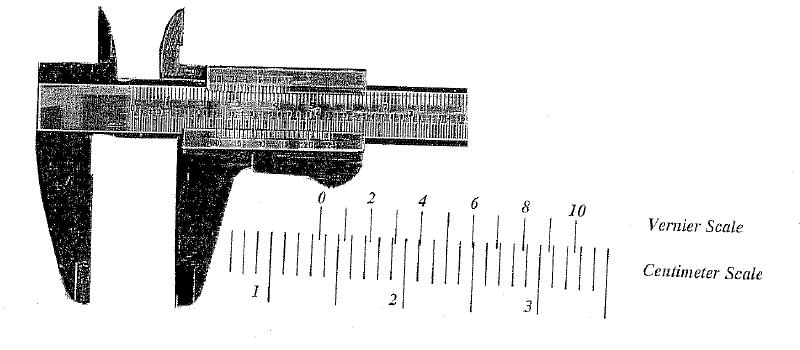
\includegraphics[width=6in]{vernier.JPG}
\vspace{-.25cm}
\caption{The Vernier Caliper:  The location of the zero on the vernier scale tells you where to read the centimeter scale (1.3 cm).  The vernier-scale line that lines up tells you the next digit (5).  This picture measures $1.35\pm 0.01 \unit{cm}$.}\label{f:vernier}
\end{center}
\begin{center}
\hspace{-2cm}
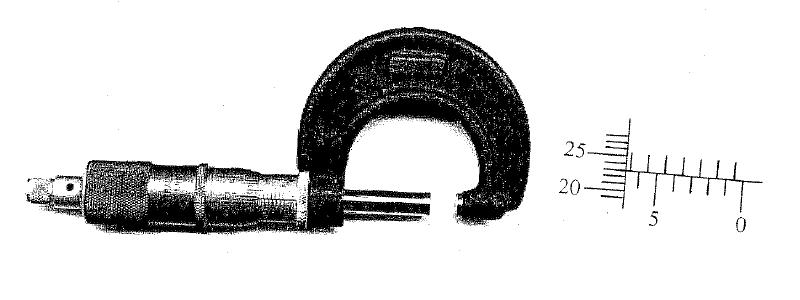
\includegraphics[width=6in]{micrometer.JPG}
\end{center}
\vspace{-.5cm}
\caption{The Micrometer Caliper:  Notice on the coarse scale, that the lower lines read (1, 2, 3, <ellipsis /> 6 in this picture) and the higher lines read the half-marks (0.5, 1.5, 2.5, <ellipsis /> 6.5 in this picture).  The location of the turning dial tells you where to read the coarse scale (6.5 mm).  The center line of the coarse scale tells you where to read the fine scale.  This is 23.0 (in units of $\times 10^{-2}$ mm), but not 23.5 and not 22.5 so the precision is 0.5 (in these units).  This measurement in mm reads $6.5 \unit{mm} + 0.230\unit{mm} = 6.730 \pm 0.005 \unit{mm}$. }\label{f:micrometer}
\vspace{-.5cm}
\end{figure}
%

%-------------------------------------------------------------------------------------
\onecolumn

\section{Standard Deviation}
\revised{Aug. 28, 2009}
\revision{Aug. 28, 2009}{Added Jack's picture back in}
\revision{Jan. 7, 1997}{Jack}

\subsection{Introduction}

Suppose you are standing in front of a dart-board.  You have a large number of darts and you throw the darts one at a time, trying to hit a 1 cm thick vertical line drawn on the dart-board.  Since you have a very good aim, let us say that 45\% of the darts hit the line.   This then means that you miss the line 55\% of the time; with a significant number of these misses being between .5 to 1.5 cm either to the left or to the right from the center of the line, and with a smaller number of misses being between 1.5 to 2.5 cm from the center line.

Is there some mathematical way of characterizing how good you are at this game?  What, for example, is the probability of missing the line by 1 cm?  The statistical analysis of random fluctuations in data can help answer these questions.   The word ``statistical'' implies that a relatively large set of similar measurements of a given physical quantity is available.  The random fluctuations in the data can be measured with the use of a mathematical term called the ``standard deviation.''

Suppose you collect data on a large number of throws, separating the data into categories (bins): The number of darts on the line, the number within .5 to 1.5 cm from the center, the number within 1.5 to 2.5 cm, etc.  A plot of this data with the dart positions on the x-axis and the number of darts hit within each bin plotted on the y-axis is called a histogram (see Figure~\ref{f:histogram}).  The envelope of this graphical data set is bell shaped, and is called a Gaussian or a Normal distribution curve.
%
\begin{figure}[bhtp]
\begin{center}
%\begin{picture}(400,200)
%\put(0,0){\line(0,1){200}}
%\put(0,0){\line(1,0){400}}
%\put(200,195){\vector(0,-1){25} $\mu$}
%\put(200,100){\vector(1,0){75}}
%\put(200,100){\vector(-1,0){75}}
%\put(200,105){$\sigma$}
%\end{picture}
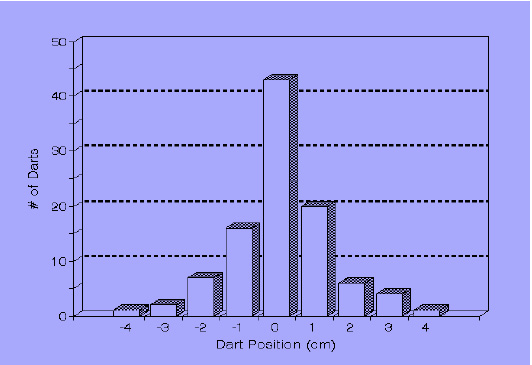
\includegraphics[height=2.5in]{darthistogram.jpg}
\caption{Histogram for the number of darts binned by distance from the centerline.}\label{f:histogram}
\end{center}
\end{figure}


The ``standard deviation'' is a measure of the spread or width of the histogram data.  A small standard deviation  means that there is a small spread in the data about the central mean value and implies that the data cluster closely about one value.   That is, there is a high degree of precision in the measurements.


The area beneath the curve, or below a part of the curve represents the probability of occurrence.  For example, the area beneath the curve between plus and minus one standard deviation from the mean represents a 68\% probability of your next throw falling within this range.  The area beneath the curve between plus and minus two standard deviations from the mean represents a 95\% probability of your next throw falling within this range.

In this experiment, you will study the use of the ``standard deviation'' in the statistical analysis and probability involved with flipping pennies.
\subsection{Experimental Purpose}

The goal of the experiment is to determine how the mean, standard deviation, and standard deviation of the mean depend on the amount of data (number of samples) taken.  You should also consider how well the data fit to a normal distribution.

\subsection{Student Outcome}

In this experiment, you should learn
\begin{enumerate}
\item the formulas for and the roles of the mean, the standard deviation, and the standard deviation of the mean in the statistical analysis of data containing random errors,
\item how to create histograms and scatter plots,
\item how to include trendlines on scatter plots, and
\item why more data is always better.
\end{enumerate}

\subsection{Pre-Lab Work}
\begin{lablist}
\item Define the following, both in a sentence and with a mathematical formula:  mean, standard deviation (sometimes called the standard deviation of a single observation), and standard deviation of the mean.  Be sure to describe the difference between these two terms.
\item Define the following:  histogram, probability, \& probability distribution (Normal distribution).
\item What does the total area under the Normal distribution curve represent?
\item How should the axes of the histogram of the data you will take for this lab be labeled?  Give a very specific scale for the x-axis.  (Hint: Read the procedure below.)
\item Make a sketch of an inverse function, like $y=1/x$.
\end{lablist}

%\twocolumn[\vspace{-.5cm}
\subsection{Experimental Procedure}

Each individual will receive 20 pennies and will then simultaneously toss all of the pennies.  Count the number of heads, and repeat 25 times.   Each individual will then have collected 25 pieces of data.
%\\]

\subsection{Analysis}

\begin{lablist}
\item Calculate the mean, the standard deviation  and the standard deviation of the mean for your first ten tosses and for all 25 tosses.  Show your calculations.
\item Make a histogram plot (by hand in your note book) for your 25 tosses.   On this histogram superimpose a sketch of your best guess of the corresponding Normal distribution curve.
\item How well does your data fit a normal distribution curve?  Explain the reasons for any large discrepancies.
\item Obtain histograms and calculations of the mean, the standard deviation and the standard deviation of the mean for the following data sets:  i) your lab group,  ii) about 1/2 of the class, and iii) the entire class.   These histograms can be obtained with the use of a computer program, provided by the instructor.
\item Draw graphs of:  the mean, the standard deviation, the standard deviation of the mean, versus the number of data entries.   Use the standard deviation of the mean  as the error bars for both the mean and the standard deviation,  draw these error bars on these two graphs.
\item Describe how the values of the mean, the standard deviation, and the standard deviation of the mean, change as the number of data items in the set increases.  What does this infer about the accuracy and about the precision of the data as more and more observations are made?
\item Show that the standard deviation of the mean varies inversely as the square root of the number of data items in the sample.   How well does the data in this lab agree with this prediction?   (Make a graph of the standard deviation of the mean versus the square root of the number of data items in the sample.)
\end{lablist}

\subsection{Questions}
\begin{enumerate}
\item What is the probability of flipping the 20 pennies and getting 5 heads, or 8 heads, or 10 heads, or 15 heads?   Answer this question by analyzing your data, the entire class' data and the normal distribution curve fit to your data.  Explain any differences between these sets.
\item What percentage of your individual readings fall within plus or minus one standard deviation,  two standard deviations?   Compare your answer to the theoretical answer from a normal distribution curve.  What are the percentages for the class data?
\item Does the height of the histograms change as a function of the number of trials?  If so, how?
\item How does the width at 1/2 the maximum height for the histograms change as a function of the number of trials?  Label this width on your histograms.  Is this width a reasonable estimate of the standard deviation?
\item Does the standard deviation of a single observation and/or does the standard deviation of the mean change significantly as the number of tosses increase?  What does this infer about the accuracy and about the precision of the data as more and more observations are made?
\end{enumerate}

\subsection*{Resource Materials}

Meyer, \underline{Data Analysis for Scientists and Engineers} John Wiley, (1975) p.19-48, 223-253


%-------------------------------------------------------------------------------------
\onecolumn

<chapter><title>Constant Acceleration</title>
<!-- Revisions
\revised{Sept. 14, 2015}
\revision{Sept. 14, 2015}{Commented out Graphs and Tracks.  Updated Pasco Reference from DataStudio to Capstone}
\revision{Sept. 16, 2008}{Created?}
-->

    <objectives><title>Experimental Purpose</title>
    <introduction><p>Using position versus time and velocity versus time graphs, verify that the equations of constant acceleration accurately describes the behavior of objects under constant acceleration and that it is possible to distinguish acceleration due to gravity from acceleration due to friction.</p>
    </introduction>
    </objectives>

    <section><title>Student Outcomes</title>
    <p>In this exercise, the student should develop an understanding of the relationships between the position and the instantaneous velocity of an object, as well as how each of these can vary as functions of time.   We will only consider the special case where the object experiences constant acceleration.</p>

    </section>

    <section><title>Materials</title>
    <p>An aluminum track, a low-friction cart, computer interface with PASCO Capstone<m>^{\rm tm}</m> software, a sonic motion sensor, a small steel ball.</p>
    </section>

    <section><title>Procedure (to be paired with Section~\ref{ss:AccAnalysis})</title>

    <subsection><title>Cart and Flat Track</title>\label{sss:FlatTrack}
    <p>Log into the computer (so you can save your data to your network drive) and then open Pasco Capstone.
    (Section~\ref{s:Capstone} will provide some instructions for setting up the software and connecting the equipment.)
Connect the motion sensor to the computer interface.
Set the data rate of the motion sensor at <m>50 \unit{Hz}</m>.
Place a steel ball on the track and adjust the leveling screw at one end of the track to see if the ball rolls one way or the other.  This will roughly level your track.
Place the sensor about 20 cm from the end of the track, because this is the minimum distance detected by the sensor.  (You might need to use the <q>sail</q> for the sensor to see the cart.)</p>

    <p>Place the cart on the track.  Capstone, via the sonic ranger, can measure the position and velocity of the cart as a function of time.  (This is explained in Section~\ref{s:Capstone}.)
<ol>
<li><p> Assume the track is frictionless and predict how the cart will move if the track is not perfectly level; include a comment about how the velocity versus time graph will look when it goes uphill versus when it goes downhill.  Should these be the same?
</p></li> <li><p> What do you expect the graph to look like if the track <em>is</em> perfectly level?  Will it be the same going left versus going right?
</p></li> <li><p> Now, assuming it is perfectly level, what will friction do to the motion?  How do you expect this to affect the graphs?
</p></li> </ol>
\setcounter{dave}{\theenumi}
</p>

    <p>We will take four sets of data: a slow, constant velocity towards the ranger; a slow, constant velocity away from the ranger; a faster, constant velocity towards the ranger; and a faster, constant velocity away from the ranger.  The two slow speeds should be about the same and the two faster speeds should be about the same.  For each case, start the sonic ranger and then bump the cart firmly, but not violently(!).</p>

    <p>On Capstone, you should have four curves of velocity versus time.  Fit each with a trendline and display the equation of the trendline on the screen.  Interpret the coefficients (slope and intercept) by noting their units, values, and uncertainties.  You should also print out (in landscape mode) the position versus time graph, the velocity versus time graph, and the acceleration versus time graph.  (You should notice that the acceleration versus time graph is <em>very</em> noisy.)</p>

    </subsection>
    <subsection><title>Cart and Sloped Track</title>\label{sss:SlopedTrack}
    <p>Place a small block under one end of the track, so that the track is now tilted at a small angle with the sensor at the top of the incline.  Measure the angle using a protractor or calculate it by measuring the two legs of the triangle and using the inverse sine.  (Be careful about measuring the height.)</p>

    <p.>We will consider <em>three cases</em> for the sloped track: <em>First</em>, allow the cart to roll (without an initial push) down the ramp.  <em>Second</em>, gently push the cart down the ramp.  DON'T let it fly off or crash into anything.
<ol>
\setcounter{enumi}{\thedave}
<li><p> Should these two cases have the same acceleration while rolling down the ramp?  How will that affect the shape of the velocity versus time graphs?
</p></li> <li><p> Should these have the same initial velocity?  How will that affect the graphs?
</p></li> </ol>
\setcounter{dave}{\theenumi}
In the <em>third</em> case, start the cart at the bottom of the incline and roll it up the ramp, allowing it to roll back down on its own.  Push it hard enough to get mostly up the ramp, but not so hard that it hits the sonic ranger.
<ol>
\setcounter{enumi}{\thedave}
<li><p> Should this case have the same acceleration while it goes up the ramp as while it goes down the ramp? How can we see that on the velocity versus time graphs?
</p></li> <li><p> Should this case have the same acceleration (either while it goes up the ramp or while it goes down the ramp) as the previous two cases of rolling down the ramp?
</p></li> </ol>
\setcounter{dave}{\theenumi}
</p>

    <p>In Capstone, you should be able to display all three graphs (position v time, velocity v time, and acceleration v time).  You should also be able to display all three cases of data on each of these graphs.  On the velocity versus time graph, fit each of the three graphs with a linear trendline.  The next section will ask you to analyze how well the data match up to these lines.  (It might be interesting to also fit the position vs time curves to parabolas.  Be sure to print out copies of your three graphs.</p>

    <p>Your lab should note the following results and explain their meaning:  slope and y-intercept, the uncertainties (precision) in both the slope and intercept, and the <m>r</m> value (correlation coefficient). </p>

    </subsection>
    </section>

    <section><title>Further Analysis and Discussion</title>\label{ss:AccAnalysis}

    <subsection><title>Cart and Flat Track</title>

    <p>Based on the results of Sec.~\ref{sss:FlatTrack}, write a short analysis of the relationship between these two graphs (x and v versus time).   From the velocity versus time graph (specifically from the trendline) determine the value of the acceleration of the cart down the track; be sure to include the uncertainty of the acceleration and the units.
<ol>
<li><p> Do you see any evidence that the track was not perfectly level?
</p></li> <li><p> Do you see any evidence that there is any friction as the cart moves along the track?
</p></li> <li><p> What does the intercept of the velocity versus time graph tell you?
</p></li> <li><p> If the slopes are different, then discuss any pattern that you see.  If the slopes are (essentially) the same, then find an average and a standard deviation of the four values.
</p></li> <li><p> Does it matter how fast the cart travels?
</p></li> </ol>
\setcounter{dave}{\theenumi}
    Discuss any evidence observed in your data when answering these questions.  Also consider the magnitude of the uncertainties when writing your conclusions.</p>

    </subsection>
    <subsection><title>Cart and Sloped Track</title>

    <p>Based on the results of Sec.~\ref{sss:SlopedTrack}, write an analysis of the relationship between the two graphs
(x and v versus time).  From the velocity versus time graph determine the value of the acceleration of the cart down the track.
<ol>
\setcounter{enumi}{\thedave}
<li><p> For the two downhill cases, use your uncertainty analysis to determine if the acceleration of the cart changed when it was given a small push.
%</p></li> <li><p> For the case that you copied into Excel, compare the results for the acceleration (with uncertainties) between <q>Data Studio</q> and Excel.  Comment on any differences.
</p></li> <li><p> Is there an accuracy<fn>If the track were frictionless, then the acceleration should be <m>a=(9.81\unitfrac{m}{s^2})(\sin\theta)</m>, where <m>\theta</m> is the angle that the incline makes.</fn> that can be computed for this part of the experiment?
</p></li> </ol>
\setcounter{dave}{\theenumi}
%
Inspect the line/curve that is defined by the data on the Distance traveled vs. time graph.
<ol>
\setcounter{enumi}{\thedave}
<li><p> What is its shape?  Is the shape of the graph what you would expect for constant acceleration (straight line, parabola, etc.)?  Explain your reasoning.
</p></li> <li><p> Consider the trendline that you added.  Does/should the trendline line go through the origin?  What is the value of y-intercept of the X vs T graph?  What physical quantity does the intercept represent?  Explain why it has that value.  Hint: (Think about where the sensor was located.)
</p></li> <li><p> What does the slope (whether it's constant or not) of the line on this graph signify?
</p></li> </ol>
\setcounter{dave}{\theenumi}
Now consider the Instantaneous Velocity  vs. Time graph.
<ol>
\setcounter{enumi}{\thedave}
<li><p> Does the curve/line on this graph have the shape you would expect for an object undergoing constant acceleration? Explain.
</p></li> <li><p> What was the value of the y intercept on this graph (include units and uncertainty!)?  Explain its significance.  To what does it refer?  Think carefully about what you plotted on the X-axis!
</p></li> </ol>
    </p>

    </subsection>
    </section>
</chapter>

%-------------------------------------------------------------------------------------
\onecolumn

<chapter><title>Newton's <m>2^{\rm nd}</m> Law on a Linear Track with the Sonic Ranger</title>\label{s:Newton}
<!-- Revisions
\revised{Sept. 14, 2015}
\revision{Sept. 14, 2015}{Updated Pasco Reference from DataStudio to Capstone}
\revision{Sept.~23, 2008}{}
-->

<introduction><title></title>Introduction to Forces}

Forces are related to the natural motion of bodies, where one object can affect the motion of another object.  That is, forces are interactions between objects affecting their motion.  Although the famous Greek philosopher Aristotle claimed that a force was necessary to <em>maintain</em> any motion, careful analysis by Italian physicist Galileo Galilei in the mid-<m>17^{\rm th}</m> century and by Sir Isaac Newton, a British mathematician and physicist (1642-1727), eventually distinguished the effects of friction and allowed Newton to create a mathematically consistent theory of motion.  These concepts were published in Newton's book <q>Mathematical Principles of Natural Philosophy</q> in 1687, for which (among other accomplishments) Newton is regarded as one of the greatest scientists of all time.

All forces can be placed in one of two main categories.  First, there are natural (or fundamental) forces like the gravitational force, the electromagnetic force, or the nuclear forces.  The gravitational force is a force on a body by another body (like the Earth), this force is an interaction between their two masses.  The electromagnetic force is an interaction between the charges of two bodies.  These forces may act on an object without any direct physical contact between the two bodies.  This type of force is sometimes called an <q>action at a distance</q> force.  All other forces are in a second category called <q>contact forces.</q>

<subsection><title></title>Newton's First law}

<quote>
If there are no forces acting, then objects will remain at rest or, if not at rest, will maintain their velocity.
</quote>
If this is true, then we can study the forces acting on a body based on the motion of the body, specifically through the change in the velocity of an object.

</subsection>
<subsection><title></title>Newton's Second Law}

Not only is a force necessary to change the motion (to cause an acceleration), the amount of acceleration that a force causes is predictable and is inversely proportional to the mass.  The same sized force causes a small mass to accelerate a lot and a large mass to accelerate a little.  this is expressed by the equation:
<me> \vec F_{\rm net} = m \vec a. </me>
The net force, <m>\vec F_{\rm net}</m>, is the vector sum of all forces acting on an object.  If we have an extended object (such as a weight hanging off of a table, but connected to a cart that is on the table), then we need only consider forces that are <q>external</q> to the system:  So long as both objects accelerate at the same rate, we do not need to consider the <q>internal</q> tension that the string exerts between the connected bodies.

</subsection>
<subsection><title></title>Newton's Third Law}

Inherent in the description of a force is that it is an interaction between objects: there must always be two objects that interact.  These objects exert equal and opposite forces on each other.  That is,
<quote>
If there is a force exerted on object 1 by object 2, then there is necessarily and simultaneously a force exerted on object 2 by object 1 that is equal (in magnitude) and opposite (in direction) to the original force.
</quote>
Remember that these two forces are on different objects and that the two bodies in direct contact exert forces on each other.  Remember then that if there is contact between the object (any part of the system) and anything else then there is an outside force on the object (system) and that if there is no contact (the two bodies break contact) then there is no force.


</subsection>
</introduction>
    <objectives><title>Experimental Objective</title>

    <introduction><p>In this experiment, we will assume that the first law is true and focus on the second law.
    By measuring (a) the velocity versus time for a cart being pulled down a track and (b) the applied force that is pulling it, we can plot the acceleration versus the force and verify the validity of Newton's second law of motion: <m>\vec F_{\rm net} = m \vec a</m>.</p>
    </introduction>
    </objectives>

</section><section><title></title>The Experimental Setup}

<ul>
<li><p> A low-friction linear cart and track will be used, this reduces the friction between the cart and the track.
</p></li> <li><p> A string will be connected to the cart and a known mass will be hanging from the end of the string (and over a pulley).   The hanging mass will exert a constant horizontal force on the cart as the mass falls all the way to the floor.  This gives a constant acceleration to the cart.
</p></li> <li><p> The sonic motion sensor will be used to measure the position of the cart as a function of time.
</p></li> <li><p> The carts and tracks need to be handled with care.  Scratches can add friction to the system.
</p></li> </ul>

</section><section><title></title>Pre-Lab Work}

<ul>
<li><p> Draw a free-body force diagram for the cart and for the hanging mass.
</p></li> <li><p> Derive an equation for the acceleration of the system, in terms of, the mass of the cart and the hanging body.
</p></li> </ul>

</section><section><title></title>Procedure}

<ul>
<li><p> If the cart is given an initial push (without the hanging mass and string attached) then the cart should travel with a constant velocity down the horizontal track, if there are no other forces acting on the cart.  Carry out  a couple of constant velocity runs on the track, to check for the effects of friction and to see how level the track is. The track may need a level adjustment.  Do runs in both directions.  Maybe the track can be tilted so that the friction is countered by the tilt of the track.
</p></li> <li><p> Connect a string to the cart and run it through the hole at the end of the track, then over a pulley.  Make sure that the string is horizontal.  Measure the height of the string at both ends of the track, to see if the string is horizontal.
</p></li> <li><p> The hanging mass should be much less than the mass of the cart.  Use a small plastic cup to hold the hanging masses.   Measure the mass of  this cup.  The total mass of the system must be kept constant for all parts of the experiment.   The hanging mass and the mass of the cart should vary, but their total must be kept constant, by moving small mass amounts from the cart to the hanging cup.  Record the mass of the cart, the hanging cup mass, and the extra masses which are to be transferred from the cart to the cup.
</p></li> <li><p> Take data with Capstone and the motion sensor as the cart travels with constant acceleration down the track.   Determine the acceleration of the cart from a linear regression using the velocity vs time data (a linear fit line in Capstone).  Record the acceleration value and its uncertainty.
</p></li> <li><p> Collect  7 data runs, where about 5 grams is transferred each time from the cart to the hanging mass.   Determine the acceleration of the cart (and the uncertainty for the acceleration) for each of these 7 runs.
</p></li> </ul>

</section><section><title></title>Analysis}

<ul>
<li><p> Make a graph of the acceleration of the system (y-axis) versus the weight (<m>mg</m>) of the hanging body (x-axis),  should include 7 data points.    Do this in Excel.   Carry out a linear regression for this data set.   Quote the  slope and intercept values, their uncertainties, their p-values, and the <m>R^2</m> value.     Show a sample error bar (on the graph) for at least one of the points of this graph.
</p></li> <li><p> Derive (show it completely)  an equation for the acceleration of the system versus the weight of the hanging body.  Plot this theory equation on your graph (as a second series, a line but no points).
</p></li> <li><p> Compare your graph to the predicted theoretical equation, that is compare the values of the slopes and intercepts.  What is the physical significance of the slope and of the intercept from the graph?  That is, what physical quantity does the slope of this graph equal?
</p></li> <li><p> In many mechanics experiments, there may be deviations from the expected or theoretical results because of the effects of friction.  Frictional forces are sometimes difficult to take into consideration.  If there are deviations between your results and the predicted theory then try to distinguish whether they are caused by a tilt of the track, friction between the cart and the track or the friction between the string and the pulley.  What might be expected in the results from these different systematic effects?    That is, would the slope be expected to increase or decrease slightly because of the effects of friction?
</p></li> <li><p> When designing experiments, it is important to keep control parameters; in this case a parameter which is kept constant.   What parameter held this role in this experiment?
</p></li></ul>

%\vfill\hfill(<m>\hookrightarrow</m>)
%\onecolumn
</section><section><title></title>Questions}

<ol>
<li><p> Why is it important to keep the total mass of the system constant?   What would happen if the total mass of the system was not held constant?    If one simply added mass to the hanger without keeping the system's mass constant,  how would their data appear on the graph of the acceleration vs <m>mg</m>?
</p></li> <li><p> What would happen if the track was not level?   If the beginning end of the track is higher,  how would the acceleration of the system be affected?
</p></li> <li><p> If your group has a discrepancy between the results and the theory, could friction be used to explain your results?   Explain how.   In this case, how much of a tilt in the air track would be needed to explain the discrepancy?   Show this calculation.
</p></li> <li><p> What would happen to the cart's acceleration if the cart was given an initial push?
</p></li> <li><p> What are the two greatest sources of uncertainty in this experiment?   Are they random or systematic errors?   Be specific and quantify your answer.
</p></li> </ol>


</chapter>

%-------------------------------------------------------------------------------------
\onecolumn

<chapter><title>Dry Sliding Friction</title>
<!-- Revisions
\revised{Sept.~28, 2015}
\revision{Sept.~28, 2015}{}
\revision{Sept.~23, 2008}{}
-->

<introduction><title></title>Introduction}

Friction is a force which retards the relative motion of any body while sliding over another body.  The frictional force acting on a body is parallel to the surface that the object is sliding upon and it is directed opposite to the direction of motion.  The phenomenon of friction is rather complicated, especially at the microscopic level, because it is dependent on the nature of the materials of both contacting surfaces.  The frictional force depends on the roughness or the irregularities of both surfaces.  At the macroscopic level, the nature of this force can be described by a simple empirical law, first given by Leonardo da Vinci:
<quote>
The magnitude of the force of friction between unlubricated, dry surfaces sliding one over the other is proportional to the normal force pressing the surfaces together and is independent of the (macroscopic) area of contact and of the relative speed.
</quote>
At the microscopic level, the frictional force <m>(F_f)</m> does depend on the actual area of contact of the irregularities of the surfaces.  This actual area of contact then increases as the force pressing the two surfaces together increases, this force is called the load.  Using Newton's <m>2^{\rm nd}</m> Law in this perpendicular direction we can conclude that the magnitude of the load is equal to the Normal force <m>(F_N)</m> of the surface pushing on the object.  Therefore we may write that
%
<me>
F_f \propto F_N
\mbox{\ \ \ \ or \ \ \ \ }
F_f = \mu F_N
</me>
%
where the Greek letter <m>\mu</m> (<q>mew</q>) is a dimensionless constant of proportionality called the coefficient of friction.

When a body is pushed or pulled parallel to the surface of contact and no motion occurs, we can conclude that the force of the push or pull is equal to the frictional force, using Newton's <m>2^{\rm nd}</m> Law of motion.  As the applied force is increased, the frictional force remains equal to the applied force until motion results.  At this maximum value of the applied force, the frictional force is also a maximum and is given by
%
<me>
F_f = \mu_s F_N
</me>
%
where the subscript <m>s</m> stands for static (non-moving) friction.  This equation can only be used at this maximum static point also called the point of impending motion.  At the instant that the applied force becomes greater than the maximum fs, the body is set into motion and this motion is opposed by a frictional force called the kinetic (sliding) frictional force and is given by
%
<me>
F_f = \mu_k F_N
</me>
%
where the subscript <m>k</m> stands for the kinetic (moving) friction.  In general, <m>\mu_k < \mu_s</m>; that is, it takes more force to overcome the static friction than to over come the kinetic friction.  The coefficients of friction are generally less than one, but may be greater than one, and they depend on the nature of both surfaces.



	Consider a system comprised of a block on a horizontal surface being pulled horizontally by a string connected to a hanging weight.   Assume that the system is accelerating with a constant acceleration.  Then the <m>\mu_k</m> can be solved for by the following equation:
%
<me>
\mu_k  = \frac{ mg - (M+m) a }{ Mg},
</me>
where <m>M</m> is the mass of the block and <m>m</m> is the hanging mass.


    </introduction>
    <objectives><title>Experimental Objective</title>

    <introduction><p>In this experiment you will devise methods to investigate the nature of both the frictional force and the coefficient of friction, and to test the validity of da Vinci's empirical rule.</p>
    </introduction>
    </objectives>

<section><title></title>Pre-Lab Analysis}

<ul>
<li><p> Draw force diagrams for the following case:     a block on a horizontal surface pulled by a hanging mass and a string  (include the friction force).
</p></li> <li><p> Write out the corresponding Newton's <m>2^{\rm nd}</m> Law equations for forces both parallel and perpendicular to the contact surface.
</p></li> <li><p> Derive the relevant equations for each of the above two cases for which the coefficients of friction can be determined:
    <ul>
    <li><p> Case one is static, but at the point of motion.
    </p></li> <li><p> Case two is the kinetic case.
    </p></li> </ul>
</p></li> </ul>


</section><section><title></title>The Experiment}

For the block on the horizontal plane:	
<ol>
<li><p> Clean the block and the plane, so that they are free of dust and other contaminants.  \\
Make sure the track is level, as in previous labs.
</p></li> </ol>
\setcounter{dave}{\theenumi}

</subsection><subsection><title></title>Break Static Friction - pull until moves}\label{sss:staticfriction}
<ol>
\setcounter{enumi}{\thedave}
<li><p> Set up the Dynamics Track, cart, force transducer and friction block.  The force transducer attaches to the dynamics cart, the friction block rests on the track (felt side down).
</p></li> <li><p>\label{i:staticpull} Attach a string to the force transducer.  The force transducer needs to be zeroed before data collection starts.  Collect data, and slowly start pulling on the string (<em>be sure to pull the string horizontally</em>) and slowly increase the pull force until the cart is moving down the track. Using just the maximum force (at the point of impending motion) the coefficient of static friction can be calculated.
</p></li> <li><p>\label{i:statictest} Test the relationship between the force of friction and the normal force, by changing the load force (normal force) and measuring the force of friction at the point of motion impending. Carry this out for a total of five data points.  Graph the frictional force versus the normal force.  Calculate the coefficient of static friction from this graph.
</p></li> </ol>
\setcounter{dave}{\theenumi}

</subsection><subsection><title></title>Effect of Surface Area - distinguish pressure from force}\label{sss:friction-area}

Consider pushing a pencil into your arm. (Well, don't <em>actually</em> do it!)  If you use the erasure end, then you can feel the force, but it doesn't hurt.  If you use the sharpened tip with the <em>same</em> force then it will certainly hurt!  So, you have the idea that the same force spread over a different surface area <em>can</em> have a different effect; but it doesn't <em>always</em> have a different effect.  For this part of the lab, you will test the relationship between the coefficient of friction and the macroscopic area of contact between the block and the surface.
<ol>
\setcounter{enumi}{\thedave}
<li><p> Place the friction block on its side (felt side down) and repeat Steps~\ref{i:staticpull} and~\ref{i:statictest} for three (rather than five) of the previous load forces.
</p></li> <li><p> Add the plot of this <m>F_f</m> versus <m>F_N</m> as a new series to the graph of Part~\ref{sss:staticfriction}.
</p></li> </ol>
\setcounter{dave}{\theenumi}

</subsection><subsection><title></title>Friction while Accelerating}

<ol>
\setcounter{enumi}{\thedave}
<li><p> Apply a force (hanging mass, pulley, and string) large enough to accelerate the block. Use the Sonic Ranger to collect data.
</p></li> <li><p> Graph the velocity vs time.  Determine the acceleration of the block from the slope of the line.
</p></li> <li><p> Repeat this part four or five times with a different normal forces.  (You may use any hanging mass.)
</p></li> <li><p> Add the plot of this <m>F_f</m> versus <m>F_N</m> as a new series to the graph of Parts~\ref{sss:staticfriction} and~\ref{sss:friction-area}.
</p></li> <li><p> Calculate the coefficient of kinetic friction from the slope.
</p></li> </ol>



</section><section><title></title>Analysis}
<ul>
<li><p> The experimental precision should be estimated for all parts of this experiment and care should be taken for all of the measurements, but it is more important to investigate the relationships than it is to repeat the experiment many times or to try to achieve high precision in the data.
</p></li> <li><p> Explain why the normal force on the block by the surface rather than the weight of the object is related to the frictional force.
</p></li> <li><p> Interpret the slope and intercept of the graphs.
</p></li> <li><p> Compare the slopes from each of the three parts.  Decide which should be the same and which should be different.
</p></li> <li><p> Calculate the \% decrease of the static to kinetic coefficient of friction.
</p></li> <li><p> Comment on the validity of the empirical rules of friction.
</p></li> </ul>


</section><section><title></title>Questions}

For all questions, and when possible, use your experimental or theoretical results to demonstrate your answers to the questions.
<ol>
<li><p> Does the coefficient of friction depend on the area of contact?
</p></li> <li><p> Does the coefficient of friction depend on the mass of the object?
</p></li> <li><p> Does the coefficient of friction depend on the normal force of the object?
</p></li> <li><p> Does the frictional force depend on the normal force of the object?
</p></li> <li><p> Does the coefficient of kinetic friction depend on the speed of travel?
</p></li> <li><p> When the object was pulled by a string, how would the forces be affected if the cord was not horizontal?
</p></li> <li><p> What would happen to the coefficient of friction if the surfaces were lubricated with oil?
</p></li> </ol>


</chapter>

%-------------------------------------------------------------------------------------


\onecolumn
<chapter><title>Centripetal Force</title>
<!-- Revisions
\revised{Fall 2006}
-->
<introduction><title></title>Introduction}

We will be investigating the force which is necessary to maintain the circular
motion of an object.
The apparatus used will allow you to spin an F-shaped arm which has a mass
suspended from the
top arm.  This mass will be held in place by a spring which makes up the lower
arm.  The spring
will provide the centripetal force.  You will need to be familiar with the
ideas of circular motion,
centripetal versus centrifugal force, centripetal acceleration, and angular
velocity.  In addition to
these concepts, try to understand how we will measure the angular speed in lab.

The centripetal acceleration <m>a_c</m> is calculated from the following equation
written either <m>\displaystyle a_c=\frac{v^2}{r}</m> or <m>\displaystyle a_c =
\omega^2 r</m>
where <m>v</m> is the linear velocity of the particle, <m>\omega</m> is the
angular velocity, and <m>r</m> is the radius of the circle.  Note that angular
velocity is measured in radians per second.

From Newton's second law, <m>\vec F = m \vec a</m>.
Therefore, the force required to keep the particle of mass <m>m</m> moving in a
circle
with constant speed is
%
<me> F = ma_c = \frac{mv^2}{r} = m\omega^2r </me>
%
Recall that the centripetal force is not a force applied <em>in addition</em> to
other existing forces.
The centripetal force is <em>whatever combination</em> of existing force act to
maintain circular motion.

    </introduction>
    <objectives><title>Purpose</title>

    <p>It is our purpose to verify the above equation experimentally by measuring the applied force
and comparing it to the specific combination of variables expressed as either
<m>\frac{mv^2}{r}</m> or <m>m\omega^2r</m>.</p>
    </introduction>
    </objectives>

<section><title></title>Pre-Lab}

<ol>
<li><p> Why do we say that an object moving with <em>constant speed</em> in a
circular path is being accelerated?
</p></li> <li><p> In which direction is that acceleration?  How do you know?
</p></li> <li><p> Is this <m>a_c</m> <q>centripetal</q> or <q>centrifugal?</q>
</p></li> </ol>

</section><section><title></title>The Experiment}

The centripetal force is supplied by a spring.  Since we cannot directly
measure <q>the
force exerted by the spring while it is rotating</q> while it is rotating,
determine how
we can measure <q>the force exerted by the spring during the
rotation</q>
when the spring is not rotating.

<ul>
<li><p>\label{i:r} By means of the lab apparatus, a mass <m>m</m> can be made to rotate with a constant (and measurable) angular speed <m>\omega</m>.  With some practice, it is possible to adjust the speed so that the radius of the path remains constant.  The value of the radius, <m>r</m>, is marked on the apparatus and so can be measured easily.
</p></li> <li><p>\label{i:m} Measuring the mass should be an obvious task.
</p></li> <li><p>\label{i:w} Measuring the angular speed <m>\omega</m> is straightforward, but may not be obvious.  To do so, consider the following:
    <ul>
    <li><p> Angular speed <m>(\omega)</m> is measured in <m>^{\rm radians}\!\!/_{\!\rm second}</m>.
    </p></li> <li><p> <m>\omega</m> is related to the rotational speed which is measured in <m>^{\rm revolutions}\!\!/_{\!\rm second}</m>.
    </p></li> <li><p> There are <m>2\pi</m> radians in 1 revolution.
    </p></li> <li><p> We can count the number of revolutions.
    </p></li> <li><p> The <q>period of rotation,</q> <m>T</m>, is defined as the number of seconds per revolution.
    </p></li> <li><p> We measure the period not by timing a single revolution, but by measuring the time for multiple (20) revolutions divided by the number of revolutions. (This averages out any uncertainty due to reaction-time.)
    </p></li> </ul>
</p></li> <li><p>[] As the mass rotates, its period of rotation can be measured.  This allows you to calculate the angular speed using the hints above.
</p></li> <li><p> Repeat the entire procedure for a second value of r.
</p></li> </ul>

</section><section><title></title>Analysis}

From measurements of <m>m</m>, <m>\omega</m>, and <m>r</m>, calculate the theoretical centripetal force on
the mass (which experimentally is supplied by the spring).  The (unmeasurable) amount
of force exerted by the spring to hold the spinning mass at a particular radius is
equal to the (measurable) force required to stretch the spring to that radius.  Experimentally determine
the force necessary to stretch the spring to a specific radius and compare that with the amount
of centripetal force calculated above.
</chapter>

%-------------------------------------------------------------------------------------

\newpage

<chapter><title>Conservation of Energy on a Linear Track</title>
<!-- Revisions
\revised{October 24, 2015}
\revision{October 24, 2015}{made it a one week lab}
\revision{August 24, 2009}{}
-->

<introduction><title>Introduction</title>

Conservation laws play a very important role in our understanding of our physical world.  For example, the law of conservation of energy can be applied in all physical processes.  This is a fundamental and independent statement about the nature of the physical world.  It is not necessarily derivable from other laws like Newton's Laws of motion.  Though for simple point mass systems, the law of conservation of energy can be derived from Newton's Laws.  It can be shown that the net work done on a system is equal to the change in the kinetic energy <m>(W_{\rm net} = \Delta K)</m> of the system; this is called the work-energy theorem and it can be written in a variety of forms.  When a net positive work is done on a system, the kinetic energy of the system increases, and when a net negative work is done on the system (as from a friction force), the kinetic energy of the system decreases.

When the gravitational force acts on a system, the work it does on the system, <m>W_g</m>, is the gravitational force <m>(mg)</m> times the vertical displacement <m>(h=\Delta y)</m>: <m>W_g=mg\Delta y</m>.  For convenience, this is called the change in gravitational potential energy <m>(W_g = - \Delta P)</m>.  <em>If</em> the gravitational force is the only force acting on the system then <m>W_g = W_{\rm net}</m> and therefore, <m>-\Delta P = \Delta K</m> for the system.  When a force can be associated with a potential energy, it is called a <q>conservative force.</q>  Another kind of potential energy deals with an elastic potential energy, like in a spring.  The energy stored in a spring is given by the formula <m>P_s = \frac{1}{2} k \Delta x^2</m>.

<em>If</em>, on the other hand, a force dissipates energy, then it is called a <q>nonconservative force</q> and it will have no associated potential energy.  Frictional forces are an example of a nonconservative force and the work done by a frictional force is negative because (physically) the frictional force removes energy from the system and (mathematically) the frictional force and the displacement are in opposite directions.  This work done by friction is converted into heat or sound.  To distinguish the energy of heat or sound from the potential and kinetic energy, we define the total mechanical energy, <m>E=K+P</m> at any point.  Since frictional forces remove mechanical energy, we say <m>W_f = \Delta E = \Delta K + \Delta P</m>.

In general then, the law of conservation of energy states that energy can not be created or destroyed, but can only change from one form to another; or the total energy of the system at point A is equal to the total energy of the system at point B.

    </introduction>
    <objectives><title>Experimental Objective</title>

    <introduction><p>The purpose of this experiment will be to verify the validity of the law of conservation of mechanical energy, that <m>\Delta E = 0</m> as a cart runs along a track.</p>
    </introduction>
    </objectives>

</section><section><title></title>The Experiment}

We would like for you to verify the conservation of mechanical energy in two different situations; so, there are two parts to this experiment.
We will first consider a flat track with accelerated motion, as in the Newton's Law lab and the Friction lab.  We can then consider an inclined plane.  You will not be given an explicit procedure, but rather you will be given a series of questions with answers that will imply the procedure.  Part of the experiment is for you to figure out for yourself what the best course of action is.  Please answer the questions as they are asked.

%There is enough analysis for this lab that you will have two weeks to complete the lab.  During the first week, you will do the two parts of the experiment and begin to write up your report.  During the second week, you will do some analysis and re-run the experiment to determine the cause of differences from expectations.  A single lab report will be due after the second week of experimentation.

</subsection><subsection><title></title>Flat Track}\label{sss:1flat}

Set up the dynamics cart on a horizontal dynamics track.  Set up the motion sensor at one end of the track and a pulley at the other end so that the pulley partly extends past the edge of the table.  Hang the basket over the pulley so that it can accelerate the cart along the track -- you might need extra weight in the cart to keep it from accelerating too fast.  In order to use this motion to verify the validity of the conservation of mechanical energy, we need to measure some variables.  Answer Questions~\ref{q:1KE} and~\ref{q:1PE} to decide on the relevant variables.  Question~\ref{q1:2or1} should help you determine how to finish setting up the equipment.

Once you decide what variables to measure, run the experiment for one set of masses while measuring the appropriate variables.  Put the data into Excel and decide what plot(s) will allow you to verify the validity of the conservation of mechanical energy.  Question~\ref{q:1plots} may help with this.  Decide if you need a trendline.  Relate the information in Question~\ref{q:1EKP} to the statement you are trying to verify.

%Save your data so that you can do further analysis next week.

</subsection><subsection><title></title>Sloped Track}\label{sss:1sloped}

Remove the pulley from the track.  Your cart will have either a spring-loaded <q>battering ram</q> on the front or a pair of magnets.  If you have the battering ram, then you will want the end of the track with the rubber nub at the bottom of the incline.  If you have the magnets, then you need to replace the pulley with a <q>C</q> shaped <q>catch-bar.</q>  <em>Ask for help from the instructor!</em>  The catch-bar has magnets in it that will repel the magnets in the cart.  In this case, the cart must not be going so fast as to come into physical contact with the magnets on the catch-bar.

Raise one end of the dynamics track.  Question~\ref{q:1slope} should help decide how tilted.  Measure the tilt angle of the track with two methods: use a protractor, and measure the vertical rise and track length and calculate the tilt angle using the inverse-sine function.  Answer Question~\ref{q:1anglemeasurement}.  As you continue to set up the track for measurements, consider answering Questions~\ref{q:1KE}, \ref{q:1PE}, and~\ref{q1:2or1} again for this situation to help you decide on the appropriate accessories (sensors); but note Question~\ref{q:1rampangle} as you think about the answers to the previous questions.

Once you decide on the variables to be measured, but before you make the measurements, you will need to calibrate your position measurements.  We would like zero to correspond to being at the bottom of the ramp, so place the cart stationary at the bottom and use the motion sensor to measure this position.  In order to verify the validity of the conservation of mechanical energy, release the cart from rest near the top of the ramp and let it roll down the incline, bouncing three times before you stop the measurement.  Do this for one value of mass.
%Answer Question~\ref{q1:mass}.

Transfer these data to Excel again and decide on the best graph to verify the objective.  Again, Question~\ref{q:1plots} may help with this; however, you will also need to consider Question~\ref{q:1bounce}.  Decide if you need a trendline and where it would be fit.  Relate the information in Question~\ref{q:1EKP} to the statement you are trying to verify.

%\newpage
</section><section><title></title>Additional Analysis}% -- Considerations during the second week}

%For the second week, you should already have your graphs from the experiment and you should have written a significant portion of the theory and the analysis.
We are now going to take a closer look at the irregularities of the data and investigate some variations to try to explain what those data say.

<ul>
%</p></li> <li><p> One of the factors you were asked to consider last week was Question~\ref{q1:mass}.  In order to verify this, re-run Part~\ref{sss:1flat} with a noticeably different massed cart.  Re-create the graph and use this only to note the effect of a different mass.  Answer Question~\ref{q1:mass2}.

<li><p> Before drawing conclusions about the validity of the conservation of mechanical energy, consider Question~\ref{q:1missing}.

%</p></li> <li><p> As you evaluate Part~\ref{sss:1sloped}, you might be asked to re-run the experiment with a force transducer placed at the bottom of the track.  (This should imply where the motion sensor will go.) Make sure that the cart will bounce from the force sensor. Make sure that the force sensor is zeroed before the start.  There might be some information here based on work as a force-through-a-distance versus work as a change-in-energy.

</p></li> <li><p> One explanation of a loss of energy (non-conservation) is friction.  List all of the places where two pieces of material rub against each other.  Since <m>F_f = \mu F_N</m>, do any of these locations have a normal force that can be varied?
    %(Recall Questions~\ref{q1:mass} and~\ref{q1:mass2}.)
    (Recall Question~\ref{q1:mass2}.)
    As an independent measure of the amount of friction, we can also consider the actual acceleration versus the expected acceleration.  Question~\ref{q:1accel} will help you determine the expected acceleration and the variable necessary to find it.  Question~\ref{q:1fracc} will help decide on the relationship between the friction and the acceleration.

</p></li> <li><p> A second explanation for the loss of energy is that some component is gaining rotational kinetic energy.  The formula for this is <m>K_R = \frac{1}{2} I \omega^2</m>, where <m>I</m> is the moment of inertia<fn>In this case, the moment of inertia is probably a little less than <m>\frac{1}{2} m r^2</m>, where <m>m</m> is the mass of the rotating object and <m>r</m> is the radius of the rotating object.  This is not a convenient way to calculate <m>I</m> at this time.</fn>, and <m>\omega</m> is the angular speed <m>\omega = v/r</m>.  Assuming that any discrepancy that you found in the conservation of energy is due to the rotational kinetic energy of the pulley, how much energy would the pulley need to have at the end of the run (while spinning full speed)?  Based on the final velocity of the cart, what is the angular speed of the pulley?  Based on these numbers, <m>K_R</m> and <m>\omega</m>, what is the moment of inertia for the pulley?   Can you tell if this is a reasonable estimate?
</p></li> </ul>


%\newpage
</section><section><title></title>Questions}

    <ol>
    <li><p>\label{q:1KE} In order to verify <m>\Delta E=0</m>, we will need to calculate <m>E</m> as <m>E=K+P</m>. Therefore, we need to know the kinetic energy, <m>K=\frac{1}{2} m v^2</m>, the energy of <em>some mass</em>, <m>m</m>, moving at a speed <m>v</m>.  Which mass do you need to measure?  How can you measure the velocity?
    </p></li> <li><p>\label{q:1PE} In order to verify <m>\Delta E=0</m>, we will need to calculate <m>E</m> as <m>E=K+P</m>. Therefore, we need to know the potential energy, <m>P=m g y</m>, the energy of <em>some mass</em>, <m>m</m>, located some height, <m>y</m>, above the ground.  Which mass do you need to measure?  How can you measure the position?
    </p></li> <li><p>\label{q1:2or1} In order to measure the position of the falling mass and the velocity of the system, do you need two motion sensors?  Can you manage with one?  Considering that it is a fairly expensive piece of equipment, where should you NOT put the sonic ranger?  Where could you put it?  Depending on where you put the ranger, decide if you need to <q>translate</q> the position or velocity data in order to find the specific values that you actually need.
    </p></li> <li><p>\label{q:1plots} To verify <m>\Delta E=0</m>, we will need to graph <m>E</m>, the total mechanical energy, as a function of time.  What do you expect this graph to look like, if the law is valid?  If not?
        <ol>
        <li><p> Does the kinetic energy change during this motion?  Is <m>\Delta K=0</m>?  Considering the initial and final values of the kinetic energy, <m>K_i</m> and <m>K_f</m>, what would a graph of <m>K</m> versus time look like?
        </p></li> <li><p> Does the potential energy change during this motion?  Is <m>\Delta P=0</m>?  Considering the initial and final values of the potential energy, <m>P_i</m> and <m>P_f</m>, what would a graph of <m>P</m> versus time look like?
        </p></li> <li><p> Assuming that the mechanical energy is conserved, what would a graph look like if it included <m>E</m>, <m>K</m>, and <m>P</m>?  What if the mechanical energy is not conserved?  How would <m>K</m> and <m>P</m> be affected in these two cases?
        </p></li> <li><p>\label{q:1bounce} (Part~\ref{sss:1sloped} only) When the cart is at the bottom of the track during the motion, the values of position become negative (less than zero!).  Why?  Is there some other place where the energy might go?  %If you are using the force transducer, then it has a spring and a spring potential energy, <m>\Delta P_{\rm spring}</m>.  This can (and should!) also be included in the total mechanical energy.  You can calculate the elastic potential energy stored in the spring of the force transducer with <m>P = \frac{1}{2} k \Delta x^2</m>, which, since we do not know <m>k</m>, can be written <m>P = \frac{1}{2} F \Delta x</m>, where F is the force in Newtons (measurable with the force transducer) and <m>\Delta x</m> is the distance from the spring's equilibrium position, not the height (derivable from the position data).  Be sure to match up the force values and the <m>x</m> values at those same times.
        </p></li> </ol>
    </p></li> <li><p>\label{q:1EKP} Please note the overall change in potential energy, <m>\Delta P</m>, and the overall change in the kinetic energy, <m>\Delta K</m>.  Should either of these be related to the overall change in energy <m>\Delta E</m> and, if so, how?
    </p></li> <li><p>\label{q:1slope}  We want the cart to accelerate down the track (not too slow), but not to fly off at the bottom (not too fast).  How fast is <em>too fast</em>?  Don't use that slope!  How fast is <em>too slow</em>?  Use a slope somewhere in between.
    </p></li> <li><p>\label{q:1anglemeasurement}  After you measure the angle of incline in these two ways, consider the uncertainty in the measurements.  Which of these measurement is more precise?
    </p></li> <li><p>\label{q:1rampangle}  The motion sensor will measure the motion of the cart <em>along</em> the ramp, but the potential energy needs the <em>vertical</em> position of the cart.  Which trig function relates the distance along the ramp to the corresponding vertical distance?
    %</p></li> <li><p>\label{q1:mass}  Does the mass of the cart matter?  If you run it again at a different value of mass, would you expect the overall conclusion to be different?  Would you expect the specific values to be different?
    </p></li> <li><p>\label{q1:mass2} If the mechanical energy is conserved, then
        <me> \frac{1}{2} m v_i^2 + m g y_i = \frac{1}{2} m v_f^2 + m g y_f </me>
        What do you notice about the mass?  Is your graph different if the mass of the cart changes?  Does this support or conflict with the idea that the total mechanical energy is conserved?  On the other hand, if the mechanical energy is not conserved, then
        <me> W_{\rm nc} = \frac{1}{2} m v_f^2 + m g y_f - \frac{1}{2} m v_i^2 - m g y_i</me>
        What do you notice about the mass now?  Does your graph support or conflict with the idea that the total mechanical energy is conserved?
    </p></li> <li><p>\label{q:1missing} We need to look for the energy lost in each graph.
        <ol>
        <li><p> When you look at the graph from Part~\ref{sss:1flat} for <m>E</m>, is the energy conserved or is there energy lost?   If lost, calculate the energy lost or gained from the graph. (It might help to have a trendline.)  If energy is lost, come up with at least two explanations for where this energy goes.
        </p></li> <li><p> When you look at the graph from Part~\ref{sss:1sloped} for <m>E</m>, there are jumps in the energy.  Why?
            <ol>
            <li><p> What is happening between the jumps?  Does Part~\ref{sss:1flat} help to explain these sections of the graph?  Compared to the jumps, can we assume that the mechanical energy is conserved between the jumps?
            </p></li> <li><p> What is happening at the time of those <q>jumps?</q>  From the trend of the graph, calculate the amount of energy lost during each sudden change, call it the energy discrepancy, and the percent of this discrepancy relative to the total energy before the corresponding collision.   Discuss where this <q>missing</q> energy goes.  Is the ratio of <q>energy discrepancy</q> to total prior energy the same for each jump?
            </p></li> </ol>
        </p></li> <li><p> Comment in general, on the law of Conservation of Mechanical Energy.  Can you predict any effects that might invalidate the conservation of mechanical energy?  Can these effects be minimized?  Is it possible to run the experiment again minimizing this effect?
        </p></li> </ol>
    </p></li> <li><p>\label{q:1accel} Given an ramp inclined at some angle <m>\theta</m>, what is the component of the gravitational force aimed down the ramp?  Assuming that there is no friction, what is the net force?  Since <m>F_{\rm net} = m a</m>, the acceleration should be <ellipsis /> ?<fn><m>a=g \sin\theta</m>.</fn>  From your expression, what do you need to measure in order to find the expected value of <m>a</m>?  (Recall Question~\ref{q:1anglemeasurement}.)
    </p></li> <li><p>\label{q:1fracc} If there is friction, then how do you expect the actual acceleration to compare to the expected acceleration?  If there is no friction?  So, how would you interpret finding an acceleration that is exactly equal to the expected value?  less than the expected value?  Larger than the expected value?
    </p></li> </ol>
</chapter>

%-------------------------------------------------------------------------------------

    \onecolumn

<chapter><title>Peer Review</title>
<!-- Revisions
\revised{Sep 1, 2008}
-->

<introduction>
<p>The most important part of doing science is the peer-review process.  After one completes a research project, the report is submitted for publication.  The publisher has a number of reviewer (usually made up of respected authors) and the submission is sent to two (sometimes three) reviewers who advise the publisher on the merits of the work.  Once you make a submission, it might be two months before the reviewers finish reviewing the work.  Generally the publisher will return the reviewers' comments to the author.  If all reviewers agree that the paper is viable, then the publisher accepts it.  If they agree not to accept a paper, then it is rejected.  If the reviewers are split, then the decision is at the discretion of the publisher.  In most cases, the reviewer makes suggestions for how to improve the paper or where to clarify the discussion.  In some cases, the author must either significantly revise the entire project or make an argument why the reviewer is either mistaken or is merely pointing out the specific point-of-contention that the author was intending to spark in the readers.  In most cases, the process of an accepted paper is
%
<ol>
<li><p> Author submits article.\label{i:submit}
</p></li> <li><p> Publishers submit to reviewers, who read and return comments to the publisher.\label{i:review}
</p></li> <li><p> Publisher gives author a chance to respond; most do (!).
</p></li> <li><p> Publishers provide authors' response to reviewers, who then give final approval (or not).
</p></li> <li><p> Paper goes to Editor, who returns paper to author for grammar, spelling, and formatting corrections.
</p></li> <li><p> After the author fixes or refuses to fix the editor's <q>suggestions,</q> the paper goes to publication.
</p></li> </ol>
%
This process can take anywhere from 1-2 months to a year and a half.  This week, we will do Step~\ref{i:submit}.  Next week, we will do Step~\ref{i:review}.</p>

<p>Usually during the review process, the reviewer is not informed of the name of the submission author -- to minimize influencing the reviewer.  Similarly, the names of the reviewers are not revealed to the submission author.  This is called <q>double-blind review.</q>  Some disciplines are specialized enough that all of the active researchers are familiar with each other's work.  In those cases, it is possible to guess who an author is (based on the approach to the project) or to guess who the reviewer is (based on the style of comments).  In principle, both sides are civil in their comments and reactions because they are members of the same community and see each other annually at the topic meetings.  Researchers are competitors and collaborators who only progress by working off of each others' ideas.</p>

</introduction>
<section><title>The Assignment</title>

<p>In order to manage the double-blind review process, before you leave lab today you will all turn in your (personally selected) code name.  Do not tell anybody what you selected and do not use a nickname that is easily recognizable by others -- the point of a secret identity is to keep the secret!</p>

<p>In this week's lab, one lab section will do Lab~\ref{s:Hooke} and the other lab section will do Lab~\ref{s:Pendulum}.  The underlying ideas are similar to each other and will help you next week when you review an article submitted by a colleague who did the other experiment.  When you submit your lab this week, you will submit your notebook and two (almost identical) copies of your report.  One copy will have your name <em>and</em> your secret code name.  The other copy will have <em>only</em> your secret identity.</p>

</section>
</chapter>

%======================================


<chapter><title>Hooke's Law and Simple Harmonic Motion</title>
<!-- Revisions
\revised{(Aug 27, 2012)}
-->
\label{s:Hooke}

<introduction><title>Introduction</title>

Oscillatory motion is one of the most common types of motions and can occur in any physical system.  Mechanical systems can experience a periodic motion, and then will vibrate at a natural frequency.  This phenomenon is called resonance.  Sound is a vibration in the air, which we hear with our ears;  light is an oscillation of electric and magnetic fields, which we can see.  The atoms and molecules in all objects are in a state of continual vibration, which we can detect as the temperature of the object, and the atomic vibrations of a quartz crystal can be used as a very accurate timer.  The study of repetitive motion is not just an intellectual exercise, but actually enables us to model complicated systems with simple harmonic motion.

In this lab, we will consider spring as an example of oscillation.  This oscillation is due to the elasticity of a spring.  We will need to measure the stiffness of the spring and relate this to the rate of oscillation.

Most systems have elastic properties, such that when the system is deformed or vibrated, there is a force which tries to restore the system to its original state.  If the restoring force is proportional to the displacement from its equilibrium position, then the object is said to be in simple harmonic motion (SHM).  A linear restoring force can be expressed mathematically by the equation
%
<me>\label{eq:hooke}
\vec F= -k\vec x \mbox{\hspace{.5cm} or as \hspace{.5cm}}  a= \frac{d^2x}{dt^2} = -\frac{kx}{m}
</me>
where <m>F</m> is the restoring force, <m>x</m> is the displacement from the equilibrium position (or zero position), <m>k</m> is a proportionality constant, and the minus sign indicates that the restoring force is always opposite the direction of the displacement.  For a spring system, <m>k</m> is called the spring constant, and represents the ratio of the applied force to the elongation.  The spring constant is an inherent physical property of the spring itself (an elastic property).  The value of <m>k</m> gives a relative indication of the stiffness of the spring.  If the spring system is in equilibrium  <m>(\sum F_i =0)</m>  then the restoring force is equal to the force pulling on the spring, and this force is proportional to the extension of the spring from its equilibrium
\end{minipage}
\hspace{.14in}
\begin{minipage}[t]{3.2in}
position.  This relationship for elastic behavior is known as Hooke's Law, after Robert Hooke (1635-1703).
%Notice that for the previous equation to be valid,  the acceleration must have the same functional form as the displacement.  One function for which this would be true is the cosine function, that is, that both the acceleration and the displacement can be represented by cosine functions.

Simple Harmonic Motion (SHM) systems can
%therefore
be described by harmonic functions (cosines), where the displacement as a function of the time <m>x(t)</m> can be written as
%
<me>	x(t) = A \cos(2\pi f t) </me>
%
where <m>A</m> is the amplitude of the motion, and <m>f</m> is the frequency of the motion in units of cycles per second (sec<m>^{-1})</m> commonly called a hertz (Hz) after Heinrich Hertz.  The period <m>(T</m>, in units of seconds per cycle) equals the inverse of the frequency <m>(f)</m>, <m>T=\phantom{1}^1\!\!/_f</m>.  For a mass on a spring, the period <m>T</m> depends on the physical parameters of the system (the mass, and the spring constant), and can be given by
%
<me>\label{eq:hookeperiod}  T=2\pi \sqrt{\frac{m}{k}} </me>
%

    </introduction>
    <section><title>Experimental Purpose</title>

Notice that Equation~(\ref{eq:hooke}) depends not only on the spring constant, but also on the acceleration (due to gravity, <m>g)</m>.  On the other hand, Equation~(\ref{eq:hookeperiod}) only depends on <m>k</m>.  You may also recall that when you measured <m>g</m> in a previous lab, you did not measure it to be <m>9.81\unitfrac{m}{s^2}</m>.  We would like our measurement of <m>k</m> to not depend on <m>g</m>.

Because of these two aspects of springs [elasticity, shown by Equation~(\ref{eq:hooke}), and periodicity shown by Equation~(\ref{eq:hookeperiod})], we can investigate both the elasticity of a spring, and use the oscillations to measure <m>g</m> indirectly.
<!--
    Experimentally determine and compare the spring constant <m>(k)</m> of a spring as determined by Hooke's Law and also with the SHM period formula.
-->
</p>
    </introduction>
    </objectives>

<section><title></title>Pre-Lab Work}

<ul>
<li><p> Make a sketch of your expectation for the displacement of a mass on a spring as a function of the time.
</p></li> <li><p> On this graph, locate and label:  the equilibrium positions <m>(x=0)</m>, and the places of maximum and minimum velocity.
</p></li> <li><p> Based on the information in the introduction, make a sketch of the pull force as a function of the displacement from the equilibrium position (initial position).
</p></li> </ul>

\end{minipage}

</section><section><title></title>Procedure}

</subsection><subsection><title></title>Hooke's law}\label{sss:hooke}
We will first measure the elasticity of the spring, using Equation~(\ref{eq:hooke}).
<ul>
<li><p> With the available spring, attach it rigidly and hang it vertically against the Dynamics Track.  Hang various masses and measure the elongation of the spring, to a maximum of 60 cm.  Do not over stretch the spring.  Record the bottom end of the mass hanger for the initial reference position.  If a tapered spring is used, the small end should be at the top.
</p></li> <li><p> Measure the elongation both when the masses are added and then when they are removed.  Perfectly elastic objects (possibly your spring) will return to the exact same location when pulled with the same force whether they are being stretched out or being allowed to relax back after stretching.
</p></li> <li><p> You will be graphing the relationship between the mass and the displacement.
</p></li> </ul>

</subsection><subsection><title></title>Oscillating Spring}\label{sss:bounce}
We will next consider the periodicity of an oscillating spring.
<ul>
<li><p> With the same range of masses as in Sec.~\ref{sss:hooke},  measure the period of oscillation for each mass.  You <em>can</em> but do not <em>have to</em> use the same values of mass, as long as the set of masses sampled are in the same range.
</p></li> <li><p> You will be graphing the relationship between the mass and the period.  I recommend using <m>T/(2\pi)</m> as the variable representing the period (because it gives nice results for the graphical parameters -- slope and intercept).
</p></li> <li><p> Advice: Keep the amplitude of vibration small,  because there is a small but measurable effect  with the period as a function of the amplitude.
</p></li> </ul>

</section><section><title></title>Analysis}

<ul>
<li><p> Graph both data sets (Sections~\ref{sss:hooke} and~\ref{sss:bounce}) in such a way that the spring constant can be determined graphically (from a linear fit model).
    <ul>
    <li><p> When you graph the relationship between the mass and the displacement, recall that Equation~(\ref{eq:hooke}) depends on two specific variables.
    </p></li> <li><p> When you graph the relationship between the mass and the period, recall that Equation~(\ref{eq:hookeperiod}) depends on one specific variable.
    </p></li> <li><p> With some effort, you should be able to recognize the units of the slope and intercept and find the relevant values.
    </p></li> </ul>
</p></li> <li><p> Physically interpret the meaning and value for the slopes, and the x and y intercepts for both graphs.
</p></li> <li><p> Calculate the spring constant for both data sets, using a linear regression method.
</p></li> <li><p> So far in the analysis, the mass of the spring has been neglected.  How would including the spring mass (or a partial \%) affect the slopes or intercepts of the two graphs?  For the period graph one would expect to get a zero period with a zero mass.  Why?  What was your observation for the  y-intercept?   If the data was modified by adding a constant amount of mass to each mass value  (say 1/3 the mass of the spring) and then re-compute the linear regression, then  what happens to the slope and intercept values?   And do you get a higher linear correlation coefficient?
</p></li> <li><p> If you assume a value for <m>g</m>, then both graphs will give you <m>k</m>.  Compare the precision for these two methods.
</p></li> <li><p> If you do not assume a value for <m>g</m>, then you can use one graph to find <m>k</m> and use this calculated value and the other graph to compute <m>g</m>.  How does this value of <m>g</m> compare to your expectations?
</p></li> <li><p> Compare the elongations when the masses were added and then removed.  Explain any differences.
</p></li> <li><p> Quantify the major sources of uncertainty in this experiment.  Which of the experimental measurements has the largest relative uncertainty?
</p></li> </ul>


</section><section><title></title>Questions}

<ol>
<li><p> Why should the amplitude of vibration be kept as small as possible?
</p></li> <li><p> Is the spring totally elastic?  (Does the elongation return to the same position when the masses are removed?)
</p></li> <li><p> Which method do you think is more precise?
</p></li> <li><p> Does the force of gravity affect the value of  <m>k</m> (as derived from each method)?  Why or  why not?
</p></li> <li><p> If this experiment were conducted on the moon, would either method give a different result for the value of <m>k</m>?  Explain.
</p></li> </ol>
</chapter>
%======================================

\newpage
\addtocounter{section}{-1}
\renewcommand{\thesection}{\arabic{section}B}
<chapter><title>The Simple Pendulum</title>
<!-- Revisions
\revised{(Aug 27, 2012)}
-->
\label{s:Pendulum}

<introduction><title>Introduction</title>

A simple pendulum consists of a small bob of mass <m>(m)</m> suspended by a light (assumed to be massless) string of length <m>(L)</m>, and the string is firmly attached at its upper end.  This pendulum is a mechanical system which we will assume exhibits simple harmonic motion.  That is, the restoring force on the pendulum is proportional to the displacement from the equilibrium position.

Oscillatory motion is one of the most common types of motions and can occur in any physical system.  Mechanical systems can experience a periodic motion, and then will vibrate at a natural frequency.  This phenomenon is called resonance.  Sound is a vibration in the air, which we hear with our ears;  light is an oscillation of electric and magnetic fields, which we can see.  The atoms and molecules in all objects are in a state of continual vibration, which we can detect as the temperature of the object, and the atomic vibrations of a quartz crystal can be used as a very accurate timer.  The study of repetitive motion is not just an intellectual exercise, but actually enables us to model complicated systems with simple harmonic motion.

Galileo (1564-1642) investigated the natural motions of a simple pendulum.  From his observations he concluded that <q>vibrations of very large and very small amplitude all occupy the same time.</q>   Galileo's time interval of measurement was his own pulse rate.  With today's modern technology we have much more precise measuring instruments.   This experiment will investigate the relationships between the physical characteristics of the pendulum and the period of the pendulum.


    </introduction>
    <section><title>Experimental Objectives</title>

<introduction><p>
<ul>
<li><p> Determine the relationship between the period of the pendulum and its amplitude.
</p></li> <li><p> Determine the relationship between the period of the pendulum and its mass.
</p></li> <li><p> Determine the relationship between the period of the pendulum and the length of the pendulum.
</p></li> <li><p> Use a graphical analysis to investigate these relationships, and from the best linear graph determine an empirical equation for the period of a pendulum.
</p></li> <li><p> Gravity also plays a part in this experiment, so include gravity into your empirical equation, and use unit analysis to help figure out this relationship.
</p></li> </ul>
</p>
    </introduction>
    </objectives>

<section><title></title>Procedure}

You will have available for your use:  pendulum bobs, string, timers, and a protractor.  Be careful to fix the string to a point of support which will not move or vibrate as the pendulum swings.  You will test each of the three relationships above (period vs amplitude, vs mass, and vs length).  While measuring one relationship, you should ensure that -- if they matter -- then the other two variables are not varied.  For example, when changing the pendulum mass do not vary the pendulum's length or its amplitude.

Some considerations while doing this lab:
<ul>
<li><p> The amplitude of oscillation is the maximum angle which the string makes with the vertical.
</p></li> <li><p> In general when testing the mass or the length, it is best to keep the amplitude of oscillation small.
</p></li> <li><p> When testing any of the relationships, you should measure a few widely-separated values.  If these seem to vary significantly, then fill in the gaps between those measurements to make a reliable graph.  See question~\ref{q:howmany}.
</p></li> <li><p> If you can prove that the period is not affected by one of these variables, then you do not need to worry about keeping it constant while you measure the other variables.
</p></li> <li><p> Your graphical analysis will be better if your graph is linear.  Consider question~\ref{q:linpend} for advice on making your graphs.
</p></li> </ul>

</section><section><title></title>Questions}

<ol>
<li><p> Was Galileo's statement precise?
</p></li> <li><p> Does this pendulum follow simple harmonic motion?
</p></li> <li><p>\label{q:howmany} How many observations should you take in order to obtain good data?
</p></li> <li><p> Air resistance gradually decreases the amplitude of the pendulum.  What effect does this have on the period of the pendulum?
</p></li> <li><p> What effect would stretching of the string have on your results?
</p></li> <li><p> How does gravity affect this experiment?  What would happen to the results if this experiment were conducted on the moon?
</p></li> <li><p>\label{q:linpend} If you have a parabolic graph, such as <m>y=ax^2</m>, then you might consider graphing <m>y</m> versus <m>x^2</m> to get a linear graph. What is the physical meaning of the slope and the intercept of each of your graphs?
</p></li> <li><p> Why is it a good idea to keep the amplitude of vibration small?
</p></li> <li><p> Where to and how should the pendulum length be measured?
</p></li> </ol>


</chapter>

%YOU ARE HERE

%-------------------------------------------------------------------------------------

\onecolumn
<chapter><title>Ballistic Pendulum</title>
<!-- Revisions
\revised{(Jack)}
-->


<section><title>Introduction</title>

Conservation laws will again play a significant part in this ballistic pendulum experiment.  A ballistic pendulum is a devise which has a cavity in the pendulum bob, and a small ball will be fired into and captured in this cavity.  When this happens, the initially stationary pendulum will swing about the pendulum's point of support.  During this collision between the ball and the pendulum, the momentum of the total system should be conserved from the instant just prior, to the instant just after the collision.  Physicist's hold true a general conservation law for momentum which applies in all interactions of two or more objects where there are no other outside forces acting on the system.  For collisions on the earth, the force of gravity is an outside force but momentum is still considered to be conserved if the time of the interaction is small.

The collision in this experiment is called a totally inelastic collision because after the collision the two objects are held together, they move together with a single velocity, and the kinetic energy of the system is not conserved during the collision.  Using the general conservation of momentum law for the collision described an equation can be written for the initial velocity of the ball in terms of the velocity of the system at the instant after the collision and the individual masses of the ball and the pendulum.  After the collision the pendulum and ball will swing and at the highest point in the swing they will be caught.  The KE of the system at the instant after the collision is converted totally to PE at the highest point in the swing.  The velocity of the system at the instant after the collision can then be determined using the law of conservation of energy.  Then with these two conservation laws, the initial velocity of the ball can be determined.

The initial velocity of the ball can also be determined by firing the ball horizontally off the edge of the table and analyzing the 2-dimensional projectile motion of  the ball moving under the influence of the gravitational force. This analysis involves separating the motion into its component directions, using the standard kinematic equations of motion and an appropriate set of measurements.

For these two very different techniques calculate the same initial velocity of the projectile.  An analysis and comparison of the two methods will help to illustrate the interconnections between these physics topics.

    </introduction>
    <objectives><title>Experimental Objectives</title>

    <introduction><p>To determine the initial velocity of the ballistic projectile from two different sets of experimental measurements, 1) the range and vertical height measurements of the projectile motion, and 2) through the use of the ballistic pendulum.</p>
    </introduction>
    </objectives>

<section><title></title>Pre-Lab Work}

<ul>
<li><p> Draw before and after pictures for a totally inelastic collision between two masses,  <m>m_1</m> and <m>M_2</m>.  Assume that <m>M_2</m> is initially stationary, and that <m>m_1</m> is initially moving horizontally with a velocity of  <m>v</m>.
</p></li> <li><p> For this collision, write out the conservation of momentum equation.  Solve for the shared velocity of the pair after the collision.
</p></li> <li><p> After the collision, the pendulum and ball will swing.  The KE of the pair at the instant after the collision will be converted to PE as it swings.  Write out a conservation of energy equation for this process, in terms of the mass of the pendulum and ball, the change in height of the system and the velocity of the system at the instant after the collision.
</p></li> <li><p> Combine these two conservation laws to derive an expression for the initial velocity of the ball (before the collision) to the final height of the ball and pendulum system.
</p></li> <li><p> Draw a picture of the ball's path when  fired horizontally off of a table.  Draw the ball in its initial position (at the moment it begins its free fall), and in its final position (at the moment just before it hits the floor).   Make the ball larger than its scale size so that it size can be easily seen in your picture.  On the picture label the height and the range of the projectile.  Think about whether the measurements should be taken from the top, bottom or the middle of the ball.  What part of the ball will hit the floor?  Think about this for both the horizontal and the vertical measurements.
</p></li> <li><p> For this projectile motion, use the kinematic equations of motion to derive an equation for the initial velocity of the ball in terms of the height and range measurements.
</p></li> </ul>


</section><section><title></title>Procedure}

</subsection><subsection><title></title>Projectile Motion}

<ul>
<li><p> Set-up the ballistic spring gun so that it will fire the projectile ball horizontally off the edge of the table.  Use a bubble level or the ball itself to make sure that the gun is level.  Move the pendulum out of the way.  Clamp the apparatus to the table, and use cardboard pads.   The initial velocity of the projectile can be changed by adjusting the spring tension.
</p></li> <li><p> Tape a piece of paper to the floor where the ball will land, then tape a sheet of carbon paper at this spot.
</p></li> <li><p> Be careful not to hit anything or anybody with the ballistic projectile!   Use larger pads or boxes to protect the tables and the walls.
</p></li> <li><p> Repeat the experiment for a sufficient number of trials (15-20), and calculate a standard deviation of the range.
</p></li> <li><p> Calculate the initial velocity (and uncertainty) of the projectile after taking the appropriate measurements.
</p></li> </ul>

</subsection><subsection><title></title>The Ballistic Pendulum}

The ballistic pendulum apparatus consists of three parts:  1) a ballistic spring-loaded gun for the firing of the projectile, 2) a hollow pendulum bob suspended by a light rod for catching the fired projectile, and  3) an angled platform for catching the pendulum bob at the highest position of the bob's swing.

<ul>
<li><p> When removing the ball from the pendulum, be sure to push up on the spring catch  in the pendulum so as to not to damage the pendulum.
</p></li> <li><p> The pointer on the side of the pendulum indicates the position of the center of mass of the system.
</p></li> <li><p> Do not try to take the apparatus apart, the instructor will give you the mass of the pendulum.
</p></li> <li><p> Clamp the base to the table, so that there is no relative motion of the base.
</p></li> <li><p> Fire the ball into the pendulum bob and mark the final notch position of the pendulum.
</p></li> <li><p> Repeat the experiment with a sufficient number of trials (15) so that a standard deviation of the notch positions can be obtained.
</p></li> <li><p> Measure the change in height of the pendulum's pointer from its initial position to the average notch position.  Calculate the uncertainty in this distance.
</p></li> <li><p> Calculate the initial velocity (and uncertainty) of the projectile ball.
</p></li> </ul>

</section><section><title></title>Analysis}

	Quantitatively compare the two methods. Calculate a percent difference between the two methods.  Calculate the uncertainties for the velocity in both methods (propagation of error), and also write these in a  \% form.  Which method is more precise?   Decide whether this experiment has random or systematic errors.  Discuss and show  your experimental evidence.

</section><section><title></title>Questions}

<ol>
<li><p> Under what conditions are the laws of momentum and energy conserved in this experiment?  State why.    Why is the mechanical energy not conserved during the collision?  Conclude whether the collision between the steel ball and the pendulum bob is elastic or inelastic.
</p></li> <li><p> During the collision, what percent of the kinetic energy of the ball was transferred to the combination of the pendulum and ball?   If energy is lost,  where does it go?
</p></li> <li><p> If this gun was aimed and fired vertically from the table top, would the ball hit the ceiling?  Assume a vertical height of 1.5 meters.   Show all of your work.
</p></li> <li><p> What effect does the force of gravity have on the horizontal velocity of the projectile?
</p></li> <li><p> Does the air resistance on the ball have a significant effect on the results of this experiment?
</p></li> </ol>

</chapter>
%-------------------------------------------------------------------------------------

\onecolumn

<chapter><title>Conditions of Equilibrium -- Model of a Human Forearm</title>
<!-- Revisions
\revised{(Nov 22, 2011)}
\revised{(Aug 18, 2011)}
-->

<introduction><title>Introduction</title>

Objects that are not accelerating are said to be in a state of equilibrium.  If the object is moving at a constant velocity, then it is in equilibrium.  If the object is at rest, then it is in <q>static equilibrium.</q>  These principles apply to many physical examples in engineering, architecture, and biophysics.   In particular, these principles allow one to be able to analyze and calculate the forces on the beams or the cables in a bridge or the forces at work in the muscles and bones in the human body.

The two conditions for equilibrium can be stated in equation form: First, if the body's center of mass is in translational equilibrium then it will not accelerate in any direction.
<me> \sum \vec F = 0 </me>
Secondly, if the body is in rotational equilibrium then it will not rotate about any point or axis of rotation.
<me> \sum \tau = 0</me>

For all systems such as these there is a special point called the center of mass or center of gravity of the system.  The center of mass calculation is a weighted average of the individual masses (giving more emphasis to those positions where there is more mass).  The location of this special point can be useful in determining whether the system will be in equilibrium.  For an object with uniform density, such as a half-meter stick, the center of mass is at the center of the stick.

    </introduction>
    <objectives><title>Experimental Objectives</title>

    <introduction><p>You will verify the equations for translational and rotational equilibrium by experimentally balancing the system and comparing the measurements to the results from these equations.</p>
    </introduction>
    </objectives>

<section><title></title>Prelab Work}

<ul>
<li><p> Define the following terms:  torque, lever arm, and center of mass.
</p></li> <li><p> State in a sentence, the first and second conditions of equilibrium.
%</p></li> <li><p> For a 2-dimensional system, these two conditions of equilibrium can be written in three equations,  write these 3 equations.
</p></li> <li><p> For a linear function, the slope can be determined from knowing the values of any two points, <m>(x_1,y_1)</m> and <m>(x_2,y_2)</m>.   Using these two points write out a formula for the slope of the line.
</p></li> <li><p> Draw a force diagram for a horizontal forearm as outlined in Section~\ref{ss:setup}.  Label all of the appropriate forces.
</p></li> </ul>

\newpage


</section><section><title></title>Procedure}

</subsection><subsection><title></title>Determine the Spring Constant of the Bicep Muscle}

\noindent
Before creating the forearm model, we need an equation for the force that the bicep exerts.  Since the spring models the bicep, we can use Hooke's law: <m>F = k(x-x_0)</m>, where <m>x_0</m> is the equilibrium position.  To find the force as a function of position, <m>F(x) = k x + b</m>, you will make two measurements of position and force and then determine the spring constant <m>k</m> and the intercept <m>b</m>.
    <ul>
    <li><p> Hang the spring from the vertical support so that it is easy to measure the position of the bottom of the spring.
    </p></li> <li><p> Measure the position of the bottom hook of the spring, <m>x_1</m>, with about <m>m_1=250\unit{g}</m> placed on the spring.
    Measure the position of the bottom hook of the spring, <m>x_2</m>, with about <m>m_2=850\unit{g}</m> placed on the spring.
    (If you measure from the floor, which is more convenient, then <m>k</m> will be negative.)
        <ul>
        <li><p> Parallax errors can be very significant with this measurement.  With the use of a mirror, this error can be reduced.  Hold the mirror vertically along the track and align your line of sight until the bottom hook of the spring and its mirror image are at the same level.  Then take the position readings.
        </p></li> <li><p> Each person in the group should carry out these measurements without looking at the other group members' results.  The average of these locations should be used.
        </p></li> </ul>
    </p></li> <li><p> With these two measurements, calculate the spring constant <m>k</m> as the slope of the graph of <m>F</m> versus <m>x</m>.
    You do not have to -- and should not -- actually create a graph of <m>F</m> versus <m>x</m> to do this, <em>if</em> you remember your prelab work for slope.
        <ul>
        %</p></li> <li><p> <m>A</m> is the slope and can be found from <m>\displaystyle \frac{m_2-m_1}{x_2-x_1}</m>.
        <li><p> <m>b</m> is the intercept.  Using one pair of data and your knowledge of <m>k</m>, find <m>b</m>.
        </p></li> <li><p> Determine the uncertainty in <m>k</m> and <m>b</m>.
        </p></li> <li><p> Now, with values and uncertainties for <m>k</m> and <m>b</m>, you can use <m>F=kx+b</m> to find the force that the spring thinks it is supporting.
        </p></li> </ul>
    </p></li> </ul>


\skipthis{
We can use a new version of Hooke's law to calculate the amount of force that the spring exerts by measuring the stretch of the spring (rather than by measuring the actual force).
    <ul>
    <li><p> Measure the position of the bottom hook of the spring, <m>x_1</m>, with about <m>m_1=250\unit{g}</m> placed on the spring.  Measure the position of the bottom hook of the spring, <m>x_2</m>, with <m>m_2=850\unit{g}</m> placed on the spring.
        <ul>
        <li><p> Parallax errors can be very significant with this measurement.  With the use of a mirror, this error can be reduced.  Hold the mirror vertically along the track and align your line of sight until the bottom hook of the spring and its mirror image are at the same level.  Then take the position readings.
        </p></li> <li><p> Each person in the group should carry out these measurements without looking at the other group members' results.  The average of these locations should be used.
        </p></li> </ul>
    </p></li> <li><p> With these two measurements, we can create an equation<fn>The equation is easier to calculate when you compare mass to position; but, it is easier to understand if you compare the weight (force on the spring) versus the position.  The equation above relates the position to the <em>mass</em>.</fn> that calculates the mass on the spring from the stretch of the spring:  <m>m(x) = A x + B</m>. Remember your prelab work for slope.
        <ul>
        <li><p> <m>A</m> is the slope and can be found from <m>\displaystyle \frac{m_2-m_1}{x_2-x_1}</m>.
        </p></li> <li><p> <m>B</m> is the intercept.  Using one pair of data, <m>m_1 = A x_1 +B</m>, solve this for <m>B</m>.
        </p></li> <li><p> Now, with values of <m>A</m> and <m>B</m>, you can use <m>m=Ax+B</m> to find the mass that the spring thinks it is supporting, <m>m</m>, from the location, <m>x</m>, of the spring when stretched.
        </p></li> </ul>
    </p></li> </ul>
}


</subsection><subsection><title></title>Experimental Setup for the Equilibrium Experiment}\label{ss:setup}

For our purposes, the forearm can be considered to jut out forwards from a vertical upper arm with the hand and the weight of the forearm itself pulling down while the bicep holds the forearm up.
The elbow joint is assumed to be a nearly frictionless pivot point for the forearm, allowing the forearm to rotate about the elbow.  The upper arm (the humerus) is connected to the forearm (the ulna) at the elbow, exerting a downward force on the forearm at the joint.

\begin{center}
\begin{tabular}{lll}
Human Arm & Model & Force Location \\ \hline
Forearm & half-meter stick & center of mass \\
\hfill (ulna and radius) && \\
Hand & clamp and hanger  & about <m>1\unit{cm}</m> from the far end \\
& \hfill or plastic cup & \\
Bicep Muscle & clamp and spring & <m>8.6\%</m> of the length of the forearm from the elbow \\
& \hfill (pulling up) & \hfill (about <m>4\unit{cm}</m> from the elbow) \\
Elbow (humerus) & clamp, hanger, weights & as near as possible to the elbow end \\
&& \hfill (about <m>1\unit{cm}</m> from the elbow-end)
\end{tabular}
\end{center}

\noindent
Be sure to include the weight of the clamps at each location where one is used.
%
<ul>
<li><p> Set-up a force diagram for this model of a horizontal forearm.
</p></li> <li><p> Set-up the equilibrium equations for this system.
</p></li> </ul>


</subsection><subsection><title></title>Equilibrium Experiment}
\label{ss:equilib}

You are going to do the following procedure for two different locations of the bicep muscle:  First set the bicep, as mentioned above, in the human location of about <m>4\unit{cm}</m> from the elbow.  Second, set the bicep at about <m>10\unit{cm}</m> from the elbow.  You should consider which location gives more leverage to lift the hand.

<ul>
<li><p> With your model completely set up, place a <m>50 \unit{g}</m> mass in the <q>hand.</q> <em>Experimentally</em> determine the force at the elbow necessary to balance the system and make it horizontal.  You may also change the position of the hand by small amounts if you find it easier to balance the system.  However, be sure to record the correct distances.
</p></li> <li><p> To check that the system is level, use another meter stick to measure the height from the floor <em>at each end</em> of the forearm half-meter stick.
</p></li> <li><p> Determine the force in the bicep muscle using the formula derived in the previous section as appropriate for the new position of the bottom of the hook of the spring (again using the mirror for accuracy).  Be sure to include the uncertainties!
</p></li> <li><p> Record all force locations as read directly from the <q>forearm</q> meter stick. <em>Do not subtract in your head</em> so that we can reproduce the locations later, if need be.
</p></li> <li><p> <em>Experimentally</em> determine the sensitivity of your values for force at the elbow by checking how many grams can be added or removed at the elbow while maintaining the horizontal equilibrium.
</p></li> <li><p> Since the hand is so sensitive, you should estimate roughly the sensitivity of the value of force at the hand.
</p></li> </ul>

With this data, you will verify the equations of equilibrium.

</subsection><subsection><title></title>Comparative Anatomy}
\label{ss:elephant}

Create a table that allows you to compare the values of force for the elbow, bicep, and hand for three different attachment-locations.
<ul>
<li><p> Enter the data from Sec.~\ref{ss:equilib}.  Record each position and each force.
</p></li> <li><p> Predict how the forces will change if the hand is moved a few millimeters closer to the bicep.  (Hint: Imagine carrying grocery bags at different locations on your lower arm while holding your arm in an L-shape.)
</p></li> <li><p> Move the hand in and measure the forces that make it balance.  Compare to your predictions.
</p></li> <li><p> Predict how the forces will change if the bicep is moved a few millimeters further from the elbow.  (Hint: Imagine sitting at different locations on a teeter-totter.)
</p></li> <li><p> Move the bicep away from the elbow and measure the forces that make it balance.  Compare to your predictions.
</p></li> </ul>

</section><section><title></title>Analysis}

    <ul>
    <li><p> For the forces measured or calculated in Sec.~\ref{ss:equilib}, test each of the conditions of equilibrium:
        <ul>
        <li><p> Translational Equilibrium: Show that the up forces equal the down forces to within your uncertainty.
        </p></li> <li><p> Rotational Equilibrium: Show that the clockwise torques equal the counterclockwise torques to within your uncertainty.
        </p></li> <li><p> To show that it does not matter which point you choose to calculate the summation of the torques about, choose the far end of the meter stick (near the hand) as the zero or the rotation point.
        </p></li> <li><p> If your conditions of equilibrium are not consistent, then calculate the necessary mass that should be in the hand and test this value experimentally. Discuss how well this value works.  (If you cannot get this to balance, you might check to be sure you included the weight of the forearm itself<ellipsis />)
        </p></li> </ul>
    </p></li> <li><p> Consider the forces in Sec.~\ref{ss:elephant}.
        <ul>
        <li><p> If you have three shopping bags of food at the grocery store that you want to hang from your arm as you walk to your car, should you hang the heaviest bag closest to your elbow or closest to your hand?  Explain.
        </p></li> <li><p> The location of the bicep relative to the elbow determines the leverage in pulling your hand to your chest (or for a quadruped move their feet forward for the next step).  Do you expect fast animals to have their leg muscles attached close to the joint or far from the joint?  Explain.
        </p></li> </ul>
    </p></li> </ul>


</section><section><title></title>Questions}
<ol>
<li><p> Is it necessary to have the meter stick horizontal for the system to be in equilibrium?   Why did we want to keep the arm horizontal?
</p></li> <li><p> How was the tension in the muscle affected as the position of attached muscle was moved further from the joint?   Keep the mass in the hand constant.
\skipthis{</p></li> <li><p> Consider an elephant and a gazelle.  Is either animal likely have their leg muscles connected at 8.6\% of their foreleg distance from the joint, like in humans?  Do you expect their bicep to be connected more closely to or further from their elbow?

    Note that large animals like an elephant are built for strength and not for speed.   Animals like a gazelle, are built for speed.  These properties are related to the animal's mass and the size of their bones.  But these properties are also related to where the muscles are attached to the bones.  Use your data and results to compare an elephant's leg to a gazelle's leg to explain the <q>strength</q> versus <q>speed</q> for these two animals.  For comparison, this human forearm system <q>strength</q> can be interpreted to mean that there is a greater ability to lift a larger mass (in the hand) with a smaller force applied by the muscle.  <q>Speed</q> can be interpreted to mean that a large change in the muscle tension force needed to move the limb (which is a small mass) in a short time period.
    }
</p></li> </ol>

</chapter>

%-------------------------------------------------------------------------------------

\onecolumn

<chater><title>Scaling Laws Among Biological Specimens</title>
<!-- Revisions
\revised{Oct 12, 2015}
\revision{Oct 12, 2015}{changed <q>is</q> to <q>us</q>}
\revision{Oct 21, 2008}{}
-->

    <introduction>
    <p>You will be given many animal skulls.  Measure some dimension that can be measured on all skulls.  Verify graphically (make the plot of mass versus your measured dimension) if this measurement can be reliably correlated to the mass of the skull.  We will assume that the mass of the skull is directly proportional to the overall size of the animal.  This technique allows mammalogists to gauge the size of animals when they can only find partial skeletons.</p>

When you fit this data with a trendline, the relationship might be the familiar linear relationship,
or it might instead be something else.  Some possibilities are:
<ul>
<li><p> Linear <m>\displaystyle y=mx+b</m>. In this case, you should plot the skull mass versus your measurement, determine the slope and intercept and the relevant regression data.  Discuss why the intercept might have the value that it does.
</p></li> <li><p> Geometric <m>\displaystyle y = a x^b</m>, where the coefficient <m>a</m> and the exponent <m>b</m> are to be determined.  In general, it is useful to fit your data this way first.  If you find <m>b</m> is close to an integer, then try a second fit with the appropriate polynomial.   For example, if <m>b\approx 1</m> then use a linear fit.
</p></li> <li><p> Exponential <m>\displaystyle y = a e^{bx}</m>, where the coefficient <m>a</m> and the base <m>b</m> are to be determined.
</p></li> </ul>

Excel can fit to any of these and provide you with the equation for the trendline.  However, Excel cannot provide the uncertainties unless the graph is linear.  If one uses logarithms, then we can make a power-fit trendline or an exponential-fit trendline plot as a line so that Excel can provide the slope and intercepts with uncertainties.  This will allow us to create a reliable mathematical relationship between the variables.  In general, it is true that linear regression is significantly easier than a general functional regression.

\vfill
\noindent
\begin{minipage}[t]{3in}
If your power fit is better then we can apply the logarithm to the geometric relation:
%
\begin{eqnarray*}
\ln y & = & \ln\left( a x^b \right) \\
\ln y & = & \ln a + \ln x^b \\
\ln y & = & \ln a + b \ln x \\
\ln y & = & \left[ b \right] \ln x + \left[  \ln a \right]
\end{eqnarray*}
%
In this case, it is useful to make a <q>log-log plot</q> of <m>\ln y</m> versus <m>\ln x</m>, which should be a straight line.  The slope of the log-log relation is <m>b</m>, the exponent, and the intercept of the log-log relation is <m>\ln a</m>, so that <m>e^{(\ln a)}=a</m> the coefficient.
\end{minipage}
\hfill
\begin{minipage}[t]{3in}
If your exponential fit is better then we can apply the logarithm to the exponential relation:
%
\begin{eqnarray*}
\ln y & = & \ln\left( a e^{bx} \right) \\
\ln y & = & \ln a + \ln \left( e^{bx} \right) \\
\ln y & = & \ln a + bx \ln \left( e \right) \\
\ln y & = & \left[ b \ln e \right] x + \left[ \ln a \right]
\end{eqnarray*}
%
In this case, it is useful to make a <q>semi-log plot</q> of <m>\ln y</m> versus <m>x</m>, which should be a straight line.  The slope of the semi-log relation is <m>b</m> (because <m>\ln e = 1)</m> and the intercept of the semi-log relation is <m>\ln a</m>, so that <m>e^{(\ln a)}=a</m> the coefficient.
\end{minipage}
\vfill

In biological relationships, it is common to find an exponential relationship with a base of <m>e=2.717182\cdots</m>; this is why we find it useful to use the <q>natural logarithm.</q>

Once you determine if you have an exponential or a geometric relationship, decide if there are any <q>outliers,</q> which animals those are, and justify why those data points might reasonably be excluded.  Re-fit the data after excluding the outliers.

</chapter>

%-------------------------------------------------------------------------------------
\end{document}

\onecolumn
\section{END of Previous Manual}



%-------------------------------------------------------------------------------------
%-------------------------------------------------------------------------------------

\newpage

<chapter><title>Conservation of Energy on a Linear Track - A Two-Week Lab</title>
<!-- Revisions
\revised{August 24, 2009}
-->

<introduction><title>Introduction</title>

Conservation laws play a very important role in our understanding of our physical world.  For example, the law of conservation of energy can be applied in all physical processes.  This is a fundamental and independent statement about the nature of the physical world.  It is not necessarily derivable from other laws like Newton's Laws of motion.  Though for simple point mass systems, the law of conservation of energy can be derived from Newton's Laws.  It can be shown that the net work done on a system is equal to the change in the kinetic energy <m>(W_{\rm net} = \Delta K)</m> of the system; this is called the work-energy theorem and it can be written in a variety of forms.  When a net positive work is done on a system, the kinetic energy of the system increases, and when a net negative work is done on the system (as from a friction force), the kinetic energy of the system decreases.

When the gravitational force acts on a system, the work it does on the system, <m>W_g</m>, is the gravitational force <m>(mg)</m> times the vertical displacement <m>(h=\Delta y)</m>: <m>W_g=mg\Delta y</m>.  For convenience, this is called the change in gravitational potential energy <m>(W_g = - \Delta P)</m>.  <em>If</em> the gravitational force is the only force acting on the system then <m>W_g = W_{\rm net}</m> and therefore, <m>-\Delta P = \Delta K</m> for the system.  When a force can be associated with a potential energy, it is called a <q>conservative force.</q>  Another kind of potential energy deals with an elastic potential energy, like in a spring.  The energy stored in a spring is given by the formula <m>P_s = \frac{1}{2} k \Delta x^2</m>.

<em>If</em>, on the other hand, a force dissipates energy, then it is called a <q>nonconservative force</q> and it will have no associated potential energy.  Frictional forces are an example of a nonconservative force and the work done by a frictional force is negative because (physically) the frictional force removes energy from the system and (mathematically) the frictional force and the displacement are in opposite directions.  This work done by friction is converted into heat or sound.  To distinguish the energy of heat or sound from the potential and kinetic energy, we define the total mechanical energy, <m>E=K+P</m> at any point.  Since frictional forces remove mechanical energy, we say <m>W_f = \Delta E = \Delta K + \Delta P</m>.

In general then, the law of conservation of energy states that energy can not be created or destroyed, but can only change from one form to another; or the total energy of the system at point A is equal to the total energy of the system at point B.

    </introduction>
    <objectives><title>Experimental Objective</title>

    <introduction><p>The purpose of this experiment will be to verify the validity of the law of conservation of mechanical energy, that <m>\Delta E = 0</m> as a cart runs along a track.</p>
    </introduction>
    </objectives>

<section><title></title>The Experiment}

We would like for you to verify the conservation of mechanical energy in two different situations; so, there are two parts to this experiment.
We will first consider a flat track with accelerated motion, as in the Newton's Law lab and the Friction lab.  We can then consider an inclined plane.  You will not be given an explicit procedure, but rather you will be given a series of questions with answers that will imply the procedure.  Part of the experiment is for you to figure out for yourself what the best course of action is.  Please answer the questions as they are asked.

There is enough analysis for this lab that you will have two weeks to complete the lab.  During the first week, you will do the two parts of the experiment and begin to write up your report.  During the second week, you will do some analysis and re-run the experiment to determine the cause of differences from expectations.  A single lab report will be due after the second week of experimentation.

</subsection><subsection><title></title>Flat Track}\label{sss:flat}

Set up the dynamics cart on a horizontal dynamics track.  Set up the motion sensor at one end of the track and a pulley at the other end so that the pulley partly extends past the edge of the table.  Hang the basket over the pulley so that it can accelerate the cart along the track -- you might need extra weight in the cart to keep it from accelerating too fast.  In order to use this motion to verify the validity of the conservation of mechanical energy, we need to measure some variables.  Answer Questions~\ref{q:KE} and~\ref{q:PE} to decide on the relevant variables.  Question~\ref{q:2or1} should help you determine how to finish setting up the equipment.

Once you decide what variables to measure, run the experiment for one set of masses while measuring the appropriate variables.  Put the data into Excel and decide what plot(s) will allow you to verify the validity of the conservation of mechanical energy.  Question~\ref{q:plots} may help with this.  Decide if you need a trendline.  Relate the information in Question~\ref{q:EKP} to the statement you are trying to verify.

Save your data so that you can do further analysis next week.

</subsection><subsection><title></title>Sloped Track}\label{sss:sloped}

Remove the pulley from the track.  Your cart will have either a spring-loaded <q>battering ram</q> on the front or a pair of magnets.  If you have the battering ram, then you will want the end of the track with the rubber nub at the bottom of the incline.  If you have the magnets, then you need to replace the pulley with a <q>C</q> shaped <q>catch-bar.</q>  <em>Ask for help from the instructor!</em>  The catch-bar has magnets in it that will repel the magnets in the cart.  In this case, the cart must not be going so fast as to come into physical contact with the magnets on the catch-bar.

Raise one end of the dynamics track.  Question~\ref{q:slope} should help decide how tilted.  Measure the tilt angle of the track with two methods: use a protractor, and measure the vertical rise and track length and calculate the tilt angle using the inverse-sine function.  Answer Question~\ref{q:anglemeasurement}.  As you continue to set up the track for measurements, consider answering Questions~\ref{q:KE}, \ref{q:PE}, and~\ref{q:2or1} again for this situation to help you decide on the appropriate accessories (sensors); but note Question~\ref{q:rampangle} as you think about the answers to the previous questions.

Once you decide on the variables to be measured, but before you make the measurements, you will need to calibrate your position measurements.  We would like zero to correspond to being at the bottom of the ramp, so place the cart stationary at the bottom and use the motion sensor to measure this position.  In order to verify the validity of the conservation of mechanical energy, release the cart from rest near the top of the ramp and let it roll down the incline, bouncing three times before you stop the measurement.  Do this for one value of mass.  Answer Question~\ref{q:mass}.

Transfer these data to Excel again and decide on the best graph to verify the objective.  Again, Question~\ref{q:plots} may help with this; however, you will also need to consider Question~\ref{q:bounce}.  Decide if you need a trendline and where it would be fit.  Relate the information in Question~\ref{q:EKP} to the statement you are trying to verify.

\newpage
</section><section><title></title>Additional Analysis}% -- Considerations during the second week}

For the second week, you should already have your graphs from the experiment and you should have written a significant portion of the theory and the analysis.  We are now going to take a closer look at the irregularities of the data and investigate some variations to try to explain what those data say.

<ul>
</p></li> <li><p> One of the factors you were asked to consider last week was Question~\ref{q:mass}.  In order to verify this, re-run Part~\ref{sss:flat} with a noticeably different massed cart.  Re-create the graph and use this only to note the effect of a different mass.  Answer Question~\ref{q:mass2}.

</p></li> <li><p> Before drawing conclusions about the validity of the conservation of mechanical energy, consider Question~\ref{q:missing}.

</p></li> <li><p> As you evaluate Part~\ref{sss:sloped}, you might be asked to re-run the experiment with a force transducer placed at the bottom of the track.  (This should imply where the motion sensor will go.) Make sure that the cart will bounce from the force sensor. Make sure that the force sensor is zeroed before the start.  There might be some information here based on work as a force-through-a-distance versus work as a change-in-energy.

</p></li> <li><p> One explanation of a loss of energy (non-conservation) is friction.  List all of the places where two pieces of material rub against each other.  Since <m>F_f = \mu F_N</m>, do any of these locations have a normal force that can be varied?  (Recall Questions~\ref{q:mass} and~\ref{q:mass2}.) As an independent measure of the amount of friction, we can also consider the actual acceleration versus the expected acceleration.  Question~\ref{q:accel} will help you determine the expected acceleration and the variable necessary to find it.  Question~\ref{q:fracc} will help decide on the relationship between the friction and the acceleration.

</p></li> <li><p> A second explanation for the loss of energy is that some component is gaining rotational kinetic energy.  The formula for this is <m>K_R = \frac{1}{2} I \omega^2</m>, where <m>I</m> is the moment of inertia<fn>In this case, the moment of inertia is probably a little less than <m>\frac{1}{2} m r^2</m>, where <m>m</m> is the mass of the rotating object and <m>r</m> is the radius of the rotating object.  This is not a convenient way to calculate <m>I</m> at this time.</fn>, and <m>\omega</m> is the angular speed <m>\omega = v/r</m>.  Assuming that any discrepancy that you found in the conservation of energy is due to the rotational kinetic energy of the pulley, how much energy would the pulley need to have at the end of the run (while spinning full speed)?  Based on the final velocity of the cart, what is the angular speed of the pulley?  Based on these numbers, <m>K_R</m> and <m>\omega</m>, what is the moment of inertia for the pulley?   Can you tell if this is a reasonable estimate?
</ul>


\newpage
</section><section><title></title>Questions}

<ol>
</p></li> <li><p>\label{q:KE} In order to verify <m>\Delta E=0</m>, we will need to calculate <m>E</m> as <m>E=K+P</m>. Therefore, we need to know the kinetic energy, <m>K=\frac{1}{2} m v^2</m>, the energy of <em>some mass</em>, <m>m</m>, moving at a speed <m>v</m>.  Which mass do you need to measure?  How can you measure the velocity?
</p></li> <li><p>\label{q:PE} In order to verify <m>\Delta E=0</m>, we will need to calculate <m>E</m> as <m>E=K+P</m>. Therefore, we need to know the potential energy, <m>P=m g y</m>, the energy of <em>some mass</em>, <m>m</m>, located some height, <m>y</m>, above the ground.  Which mass do you need to measure?  How can you measure the position?
</p></li> <li><p>\label{q:2or1} In order to measure the position of the falling mass and the velocity of the system, do you need two motion sensors?  Can you manage with one?  Considering that it is a fairly expensive piece of equipment, where should you NOT put the sonic ranger?  Where could you put it?  Depending on where you put the ranger, decide if you need to <q>translate</q> the position or velocity data in order to find the specific values that you actually need.
</p></li> <li><p>\label{q:plots} To verify <m>\Delta E=0</m>, we will need to graph <m>E</m>, the total mechanical energy, as a function of time.  What do you expect this graph to look like, if the law is valid?  If not?
<ol>
</p></li> <li><p> Does the kinetic energy change during this motion?  Is <m>\Delta K=0</m>?  Considering the initial and final values of the kinetic energy, <m>K_i</m> and <m>K_f</m>, what would a graph of <m>K</m> versus time look like?
</p></li> <li><p> Does the potential energy change during this motion?  Is <m>\Delta P=0</m>?  Considering the initial and final values of the potential energy, <m>P_i</m> and <m>P_f</m>, what would a graph of <m>P</m> versus time look like?
</p></li> <li><p> Assuming that the mechanical energy is conserved, what would a graph look like if it included <m>E</m>, <m>K</m>, and <m>P</m>?  What if the mechanical energy is not conserved?  How would <m>K</m> and <m>P</m> be affected in these two cases?
</p></li> <li><p>\label{q:bounce} (Part~\ref{sss:sloped} only) When the cart is at the bottom of the track during the motion, the values of position become negative (less than zero!).  Why?  If you are using the force transducer, then it has a spring and a spring potential energy, <m>\Delta P_{\rm spring}</m>.  This can (and should!) also be included in the total mechanical energy.  You can calculate the elastic potential energy stored in the spring of the force transducer with <m>P = \frac{1}{2} k \Delta x^2</m>, which, since we do not know <m>k</m>, can be written <m>P = \frac{1}{2} F \Delta x</m>, where F is the force in Newtons (measurable with the force transducer) and <m>\Delta x</m> is the distance from the spring's equilibrium position, not the height (derivable from the position data).  Be sure to match up the force values and the <m>x</m> values at those same times.
</ol>
</p></li> <li><p>\label{q:EKP} Please note the overall change in potential energy, <m>\Delta P</m>, and the overall change in the kinetic energy, <m>\Delta K</m>.  Should either of these be related to the overall change in energy <m>\Delta E</m> and, if so, how?
</p></li> <li><p>\label{q:slope}  We want the cart to accelerate down the track (not too slow), but not to fly off at the bottom (not too fast).  How fast is <em>too fast</em>?  Don't use that slope!  How fast is <em>too slow</em>?  Use a slope somewhere in between.
</p></li> <li><p>\label{q:anglemeasurement}  After you measure the angle of incline in these two ways, consider the uncertainty in the measurements.  Which of these measurement is more precise?
</p></li> <li><p>\label{q:rampangle}  The motion sensor will measure the motion of the cart <em>along</em> the ramp, but the potential energy needs the <em>vertical</em> position of the cart.  Which trig function relates the distance along the ramp to the corresponding vertical distance?
</p></li> <li><p>\label{q:mass}  Does the mass of the cart matter?  If you run it again at a different value of mass, would you expect the overall conclusion to be different?  Would you expect the specific values to be different?
</p></li> <li><p>\label{q:mass2} If the mechanical energy is conserved, then
    <me> \frac{1}{2} m v_i^2 + m g y_i = \frac{1}{2} m v_f^2 + m g y_f </me>
    What do you notice about the mass?  Is your graph different if the mass of the cart changes?  Does this support or conflict with the idea that the total mechanical energy is conserved?  On the other hand, if the mechanical energy is not conserved, then
    <me> W_{\rm nc} = \frac{1}{2} m v_f^2 + m g y_f - \frac{1}{2} m v_i^2 - m g y_i</me>
    What do you notice about the mass now?  Does your graph support or conflict with the idea that the total mechanical energy is conserved?
%\pagebreak[3]
</p></li> <li><p>\label{q:missing} We need to look for the energy lost in each graph.
<ol>
    </p></li> <li><p> When you look at the graph from Part~\ref{sss:flat} for <m>E</m>, is the energy conserved or is there energy lost?   If lost, calculate the energy lost or gained from the graph. (It might help to have a trendline.)  If energy is lost, come up with at least two explanations for where this energy goes.
    </p></li> <li><p> When you look at the graph from Part~\ref{sss:sloped} for <m>E</m>, there are jumps in the energy.  Why?
    <ol>
    </p></li> <li><p> What is happening between the jumps?  Does Part~\ref{sss:flat} help to explain these sections of the graph?  Compared to the jumps, can we assume that the mechanical energy is conserved between the jumps?
    </p></li> <li><p> What is happening at the time of those <q>jumps?</q>  From the trend of the graph, calculate the amount of energy lost during each sudden change, call it the energy discrepancy, and the percent of this discrepancy relative to the total energy before the corresponding collision.   Discuss where this <q>missing</q> energy goes.  Is the ratio of <q>energy discrepancy</q> to total prior energy the same for each jump?
    </ol>
    </p></li> <li><p> Comment in general, on the law of Conservation of Mechanical Energy.  Can you predict any effects that might invalidate the conservation of mechanical energy?  Can these effects be minimized?  Is it possible to run the experiment again minimizing this effect?
</ol>
</p></li> <li><p>\label{q:accel} Given an ramp inclined at some angle <m>\theta</m>, what is the component of the gravitational force aimed down the ramp?  Assuming that there is no friction, what is the net force?  Since <m>F_{\rm net} = m a</m>, the acceleration should be <ellipsis /> ?<fn><m>a=g \sin\theta</m>.</fn>  From your expression, what do you need to measure in order to find the expected value of <m>a</m>?  (Recall Question~\ref{q:anglemeasurement}.)
</p></li> <li><p>\label{q:fracc} If there is friction, then how do you expect the actual acceleration to compare to the expected acceleration?  If there is no friction?  So, how would you interpret finding an acceleration that is exactly equal to the expected value?  less than the expected value?  Larger than the expected value?
</ol>
</chapter>
%-------------------------------------------------------------------------------------
%-------------------------------------------------------------------------------------

\onecolumn

<chapter><title>Standing Waves on a String</title>
<!-- Revisions
\revised{(Jan, 2012)}
\revision{(Jan, 2012)}{Fixed Wavelength plots F vs v^2 to get m/L as slope.  Added comments about stretching affecting density.}
\revision{(Aug, 2011)}{Rearranged equations for clarity.}
\revision{(Jan, 2008)}{Created}
-->
\label{s:standingwaves}

<introduction><title>Introduction</title>

A wave is the propagation of a disturbance in a medium.  In a transverse wave, the disturbance of the medium is perpendicular to the direction of the propagation of the wave.  In this experiment, transverse waves will be propagated along a taut flexible string.  The frequency of the waves is determined by the source, the wave generator, which is connected to one end of the string.   The speed of the waves, <m>v</m>, is determined by the medium itself; namely the linear mass density of the string, <m>(m/L)</m>, and the tension in the string which is determined by the static force of a mass suspended from the other end of the string, <m>F_T</m>.  This is expressed by Eq.~(\ref{eq:velten}) below.

Upon hitting at the fixed end of the string, the transverse waves will reflect back along the string.  If the end of the string is rigidly held then the reflected waves will be inverted <m>180^\circ</m>.  The initial propagated waves and the reflected waves will interfere constructively and destructively.  At particular string tensions and/or wave frequencies, this wave superposition will give rise to waves called standing waves or stationary waves.  There are many different standing waves patterns (normal modes) possible which have different wavelengths.  The different modes are characterized by the number of nodes or antinodes in the wave.  At one of the normal modes of oscillation, the amplitude of oscillation can become rather large, much larger than the amplitude of the original propagated wave.  This phenomenon is called resonance.  In this experiment, each end of the string will be close to a node position.  The fundamental frequency (mode n=1) exhibits a wave pattern with one antinode.  The second harmonic (mode n=2) exhibits a wave pattern with two antinodes, and so forth.

    </introduction>
    <section><title>Experimental Objectives</title>

    <introduction><p>In this experiment, the conditions required for the production of standing waves in a string will be investigated in order to
<ul>
</p></li> <li><p>[a)] empirically verify the relationship between the frequency <m>(f)</m>, wavelength <m>(\lambda)</m>, and speed of a standing wave <m>(v)</m>, for a series of normal modes of oscillation, and
</p></li> <li><p>[b)] use the two relationships of the speed of the wave
 \begin{eqnarray}
 v & = & \sqrt{\frac{F_T}{m/L}} \label{eq:velten} \\
 v & = & \lambda f \label{eq:velwave}
 \end{eqnarray}
 to empirically relate the string tension <m>(F_T)</m> and the wave velocity <m>(v)</m>, for one mode of oscillation, specifically the fundamental mode.
</ul>
</p>
    </introduction>
    </objectives>

<section><title></title>Pre-Lab Work}

<ul>
</p></li> <li><p> Define the following terms:   standing wave, node, and antinode.
</p></li> <li><p> Draw a set of pictures of a standing wave on a string with two fixed ends showing the fundamental frequency (n=1), and the harmonics n=2, 3, 4, and 5.  Label a wavelength, the nodes, and the antinodes on each picture.
</p></li> <li><p> Given Eq.~(\ref{eq:velten}), predict what will happen to the velocity of the wave as the static hanging mass (providing the tension) increases, decreases, or stays the same.
</p></li> <li><p> Given Eq.~(\ref{eq:velwave}), how can measurements of <m>\lambda</m> and <m>f</m> be plotted to determine the wave velocity from the graph? (There is more than one way to do this; one way in particular produces a line.)  How should the axes of the graph be labeled?  Explain your reasoning.
%</p></li> <li><p> Given Eqs.~(\ref{eq:velten}) and~(\ref{eq:velwave}), create an equation that relates the tension, <m>F_T</m> to the frequency, <m>f</m>.  How would you graph this to get a line and how would you interpret the slope and intercept?
</ul>

</section><section><title></title>Fixed Tension}

In order to verify Eq.~(\ref{eq:velwave}), you can fix <m>F_T</m> and compare multiple <m>f</m> to the corresponding <m>\lambda</m>.

</subsection><subsection><title></title>Procedure}

<ul>
</p></li> <li><p> If you have not already done so, measure the mass and length of the string in order to calculate the linear mass density <m>(m/L)</m>.  You might note Question~\ref{q:stretching}.
</p></li> <li><p> A mechanical vibrator, driven with a (variable frequency) function generator, will be the wave source.  Use a string slightly greater than the length of the table.  Connect one end of the string to the vibrator and hang the other end over a pulley, keeping the string horizontal.
</p></li> <li><p> Set up the system with some particular string tension (like 450 grams).  This tension will be kept constant for this entire part.
</p></li> <li><p> Produce 5 different normal modes by changing the frequency of the vibrator.  Adjust the standing wave amplitude until it is at its maximum.  Record the corresponding frequency for each normal mode.
</p></li> <li><p> Measure the corresponding wavelengths for each normal mode, directly from the string with a meter stick.  The vibrator end of the string is not a true node because the string is vibrating a small amount.  Take this into account when measuring the wavelengths.
</p></li> <li><p> Try touching the string at a node and at an antinode.  What happens to the wave in each case?
</p></li> <li><p> Optional:  Try measuring the frequency of the vibrator with a strobe lamp.
</ul>

</subsection><subsection><title></title>Analysis}

<ul>
</p></li> <li><p> Determine the mathematical relation between the wavelength of the standing wave and the frequency of the vibrator that will produce a straight line <m>(y=mx+b)</m> when graphed.
</p></li> <li><p> Comment on the significance (and units) of the slope and intercept of this graph.  Determine both the precision and the accuracy of the slope and of the intercept; are they consistent with what you expect?  (Your expectation should be based on the <q>other</q> equation which we are not testing here.)
</p></li> <li><p> Use one or both of these (slope and intercept) to determine the velocity (with uncertainty) of the standing wave.  Relate this (\%-error) to the expected value based on the tension you chose for your specific string.
</ul>

</section><section><title></title>Fixed Wavelength}

In order to verify Eq.~(\ref{eq:velten}), you can fix <m>\lambda</m> and compare multiple <m>F_T</m> to the corresponding <m>v</m>.

</subsection><subsection><title></title>Procedure}

<ul>
</p></li> <li><p> If you have not already done so, measure the mass and length of the string in order to calculate the linear mass density <m>(m/L)</m>.  You might note Question~\ref{q:stretching}.
</p></li> <li><p> A mechanical vibrator, driven with a (variable frequency) function generator, will be the wave source.  Use a string slightly greater than the length of the table.  Connect one end of the string to the vibrator and hang the other end over a pulley, keeping the string horizontal.
</p></li> <li><p> Place 150 grams (including the hanger) on the end of the string.  (If you start with too little mass, the string stretches different amounts -- changing the string's effective density -- during the experiment, causing unaccounted for curving in the graph.)
</p></li> <li><p> Adjust the frequency of the generator until the n=2 mode is observed and is at its maximum amplitude.  Record the frequency and corresponding wave velocity.
</p></li> <li><p> Repeat the previous step for 6 hanging masses up to about 1200 grams.
</ul>


</subsection><subsection><title></title>Analysis}

<ul>
</p></li> <li><p> Determine the mathematical relation between the hanging mass <m>(F_T)</m> and the wave velocity <m>(v)</m> that will produce a straight line <m>(y=mx+b)</m> when graphed.
</p></li> <li><p> Determine which variables the slope and intercept of this graph should be related to.  Determine both the precision and the accuracy of the slope and of the intercept; are they consistent with what you expect?  (The equation we are testing should imply what to expect.)
</ul>


</section><section><title></title>Questions}

<ol>
</p></li> <li><p> What are the necessary and sufficient conditions for the production of standing waves?
</p></li> <li><p> Is it valid to consider the tightening of the string to be the same as a change of medium?  (Does tightening the string change the way waves move or the way standing waves are produced on the string?) Why or why not?
</p></li> <li><p>\label{q:stretching} When you measure the length of string, remember that the string will be under tension (pulled on) and may have some <q>give</q> to it.  It may be possible for it to stretch by nearly 10\%. If you don't account for this (if you measure the unstretched length) will your value of density be incorrect too large or incorrect too small?  Can you account for this either in the value of the length or in the uncertainty of the length.  Will this affect comparison to either of your graphs?
</p></li> <li><p> Consider the Fixed Tension graph.  We noted that the vibrator end of the string should not be considered to be a node.  This means that the node might be a little in front of the post or a little behind the post and therefore your wavelength values might be a little wrong, but your error bars should already include the amount the values could be off.  Based on the error bars on your Fixed Tension graph, would shifting the wavelength data a little larger or a little smaller have made a difference to the values of slope or intercept that you calculated?  If so, would it have increased the value or decreased the value?  If not, why not?
</p></li> <li><p> If the tension and the linear density of the string remain constant, but the pulley is shifted further from the post (so that the region which is vibrating lengthens), how is the resonant wavelength affected?  How is the velocity of the wave affected?
</p></li> <li><p> What was the experimental velocity (and uncertainty) of the waves in part I of the experiment?
</p></li> <li><p> What will happen to the velocity of the wave if the tension is fixed but the frequency is changed.
</ol>

</chapter>


%-------------------------------------------------------------------------------------

\onecolumn
\newcommand{\iftwoweek}[2]{#2}

<chapter><title>Archimedes' Principle</title>
<!-- Revisions
\revised{Nov. 23, 2008}
-->

<introduction><title>Introduction</title>

Archimedes was a Greek scientist who lived from 287-212 BCE.  As the story goes, the king thought that his crown was not pure gold and asked Archimedes to determine if this was true.   Archimedes had previously observed that a totally submerged object displaces a volume of fluid which is equal to the volume of the object, and deduced what is now called Archimedes' principle: that the buoyant force on the submerged object is equal to the weight of the displaced fluid.
Knowing the weight and density of gold, Archimedes measured the weight of the crown and the weight and volume of the water displaced by the crown, enabling him to determine that the crown was not pure gold.

As any swimmer who has had their head more than about 8 feet deep can tell you, the pressure exerted on the diver by the water increases as the diver swims deeper into the water.  We can express this as: the pressure within a fluid is dependent on the depth at which the object sits <m>(h)</m>, the gravitational acceleration of the earth <m>(g)</m>, and the density of the fluid <m>(\rho_f)</m>: <m>P=\rho_f gh</m>.  Because of this, the bottom surface of any object in a fluid will have more pressure on it than the top surface.  This <m>\Delta P</m> gives rise to a net upward force acting on the submerged object: the buoyant force <m>(F_B)</m>.  The magnitude of the upward force depends on the density of the fluid and the size of the object: <m>F_B=\rho_f g V_o</m>, where <m>V_o</m> is <em>the submerged portion</em> of the volume of the object.  A partially submerged object has a smaller buoyant force than a completely submerged object.  Interestingly, unless the fluid density depends on the depth of the fluid, the <m>F_B</m> is independent of the depth of the object.

Knowing the buoyant force will help you determine if an object will float or sink.  To determine whether an object will sink or float one should use Newton's second law to determine the direction of the net force.  Assuming the simplest case of a submerged object feeling only its weight <m>(F_g=m_og = \rho_o g V_o)</m> and the buoyant force <m>(F_B=\rho_f g V_o)</m>, if the weight of the object is greater than <m>F_B</m> then the net force on the object is down and it will sink.  If <m>F_B</m> is larger than the weight then the net force on the object is up and then it will accelerate up.  However, when an object is floating, it is in equilibrium and the object's weight is equal to <m>F_B</m>, which depends on the submerged volume.  While floating, not all of the object is submerged.


    </introduction>
    <section><title>Experimental Objectives</title>

    <introduction><p>After verifying some properties of the buoyant force using Archimedes' principle, each group will predict the maximum amount of cargo (the number of pennies) that a ship (glass beaker) will hold without sinking.</p>
    </introduction>
    </objectives>

<section><title></title>Pre-Lab Work}

<ul>
</p></li> <li><p> Using the definitions of force as pressure times area, <m>F=PA</m>, and pressure, <m>P=\rho_f g h</m>, derive the equations for the buoyant force <m>F_B=\rho_fgV_o</m> (if totally submerged) and for the object's weight <m>F_g=\rho_o gV_o</m>, where <m>\rho_o</m>  is the object's density.
</p></li> <li><p> Show that although the pressure on an object does depend on depth within the fluid, the <m>\Delta P = P_{\rm bottom}-P_{\rm top}</m> (and therefore <m>F_B)</m> is independent of the depth within the fluid.
</p></li> <li><p> Draw a force diagram for a completely submerged object:
    \begin{description}
    </p></li> <li><p>[case 1] object's density is greater than that of the fluid's,
    </p></li> <li><p>[case 2] object's density is less than that of the fluid's.
    \end{description}
</p></li> <li><p> Using Newton's Second Law show that the object in case 1 will sink, and  that the object in case 2  will accelerate up.
</p></li> <li><p> Draw a force diagram for a partially submerged object which is floating.
</p></li> <li><p> Using Newton's Second Law show that if an object has a density <m>\rho_o=.5\rho_f</m>  that only 0.5 of the object's volume is submerged.
</p></li> <li><p> Look up the density of water.
</ul>

</section><section><title></title>Procedure}

</subsection><subsection><title></title>Develop Your Understanding}

<ul>
</p></li> <li><p> Select an object for which you can easily measure the volume using a caliper.
</p></li> <li><p> Measure the dimensions and calculate the volume.
</p></li> <li><p> Measure the mass using the triple beam balance at your table.
</p></li> <li><p> Calculate the density with uncertainty.
</p></li> <li><p> Predict (with uncertainty) what buoyant force this object would have if it were completely submerged.
</p></li> <li><p> Predict (with uncertainty) what a scale would read if this object were completely submerged.
</ul>

</subsection><subsection><title></title>Verify Your Understanding}

<ul>
</p></li> <li><p> Place a balance on top of a support rod so that the side with the string dangling can drop into a container of water.
</p></li> <li><p> Find the mass of your catch beaker -- this should be a graduated cylinder because you will be using this beaker to measure both the volume and the mass of the fluid that overflows from the overflow container.
</p></li> <li><p> Place an overflow container under the scale so that the string can dip into the container if the lab jack is raised or lowered.
</p></li> <li><p> Place a catch beaker next to the overflow container and slowly fill the overflow container until it just starts dripping.  Gently tap the overflow container once.  Be very careful not to bump your table after this.
</p></li> <li><p> As thoroughly as possible, dry off your catch beaker and put it back in place.  If you cannot dry it off completely, you will not be able to accurately complete all of the necessary steps.
</p></li> <li><p> Attach your object to the string, measure the mass of the object, <m>m_o</m>, in air while the object dangles.
</p></li> <li><p> Raise the lab jack until the object is completely submerged.  <em>Be sure to catch all of the water that overflows from the container!</em>
</p></li> <li><p> The scale should now read a reduced mass, <m>m_s</m>, for the submerged object.  Record this value.
</p></li> <li><p> You now have three ways of calculating the buoyant force:  (Pay attention to which is the most precise and why.)
    <ol>
    </p></li> <li><p> \label{i:deltam} The water (via the buoyant force) supports the difference in weights between not submerged and totally submerged.  Calculate the buoyant force, with uncertainty, as the difference in these <em>weights</em>.  Does it agree with your prediction?
    </p></li> <li><p> \label{i:V_f} Measure the volume of the overflow water.  This is equal to the volume of the object submerged, <m>V_f = V_o</m>.  Calculate (with uncertainty) the buoyant force from this volume, <m>F_B = \rho_f g V_o</m>.  Does this agree with your prediction?
    </p></li> <li><p> \label{i:m_f} Note that <m>\rho_f V_f = m_f</m>, so instead of measuring <m>V_f</m>, we can measure the mass of the overflow water.  The buoyant force can also be found from:  <m>F_B = m_f g</m>, the weight of the fluid.  Does this agree with your prediction?
    </ol>
</ul>

You should ensure that you understand these results <em>with uncertainty</em> before continuing.  If this doesn't make sense, then check your numbers, check your units, remeasure quantities that you thought you were sure of, and ask your instructor.

</subsection><subsection><title></title>Consider How the Buoyant Force Changes as an Object is Submerged}

For this part, you are going to repeat the previous procedure, with three modifications.  First, you won't be able to measure the volume with a caliper.  Second, based on the previous procedure, we now know which measurement provides the best estimate (smallest uncertainty) for the buoyant force, so you should only need to do one of \ref{i:deltam}, \ref{i:V_f}, or \ref{i:m_f} from the previous section.  Finally, we will consider an object in air, partially submerged, and fully submerged.

<ul>
</p></li> <li><p> Select a fairly large object for which you cannot easily measure the volume using a caliper.  This must fit within the overflow container without touching the sides.
</p></li> <li><p> Refill the overflow container, as before, until is just starts to overflow.
</p></li> <li><p> As thoroughly as possible, dry off your catch beaker.  If you cannot dry it off, you will have to measure its mass with whatever water is in it and you will not be able to use the previous section technique \ref{i:V_f} because you cannot accurately measure the volume of new water.
</p></li> <li><p> Attach it to the string hanging from the balance and find the mass in air, <m>m_o</m>.
</p></li> <li><p> <em>You will need to do the rest of this <em>very</em> carefully.  Go slowly and do not bump the table.</em>
</p></li> <li><p> Raise the lab jack until the object is about half submerged.  Catch the overflow water.
</p></li> <li><p> Measure the apparent mass of the object and the mass or volume of the overflow water, as appropriate
    <ul>
    </p></li> <li><p> Calculate the buoyant force with uncertainty.
    </p></li> <li><p> Calculate the volume (with uncertainty) of the object that is submerged.
    </ul>
</p></li> <li><p> Without removing any of the water from the catch beaker, continue to submerge the object and catch the overflow water until the object is completely submerged.
</p></li> <li><p> Measure the new apparent mass of the object and the mass or volume of the overflow water, as appropriate.
    <ul>
    </p></li> <li><p> Calculate the buoyant force with uncertainty.
    </p></li> <li><p> Calculate the volume (with uncertainty) of the object that is submerged.
    </p></li> <li><p> Calculate the density (with uncertainty) of the object.
    </ul>
</ul>

</subsection><subsection><title></title>Fill the Cargo-Hold}

You have been provided with a beaker and some pennies.  Use the information in the previous sections to predict the maximum number of pennies that can be gently placed into the beaker without allowing it to sink.  You should measure the mass of the beaker and the dimensions of the beaker.  The volume of a cylinder is <m>V=\pi r^2 h</m>.  You should also measure about 30 pennies (all at once) to find an average mass for the pennies.

After you have calculated your prediction with uncertainty, prepare the overflow canister with water and dry the catch beaker.  Invite the instructor to your table and allow the instructor to test your prediction.


</section><section><title></title>Questions}

<ol>
</p></li> <li><p> Why does an object weigh a different amount when in air and when submerged in water?
</p></li> <li><p> If the string was cut on your first object (while submerged), what would be the acceleration of the object?
</p></li> <li><p> Why is it important to make certain that no air bubbles adhere to the object during the submerged weighing procedures?
</p></li> <li><p> What would the buoyant force be for an object that was immersed in a fluid with the same density as the object?
</p></li> <li><p> A floating barge filled with coal is in a lock along the Ohio River.   If the barge accidentally dumps its load into the water, will the water level in the lock rise or fall?
</p></li> <li><p> Does the mass of displaced water depend on the mass of the totally submerged object or on the volume of the submerged object?
</p></li> <li><p> There are two identical cargo ships.  One has a cargo of 5 tons of steel and the other has a cargo of 5 tons of styrofoam.  Which ship floats lower in the water?
</ol>









</chapter>



%-------------------------------------------------------------------------------------

\onecolumn

<chapter><title>Centripetal Force</title>
<!-- Revisions
\revised{Fall 2006}
-->

<section><title>Introduction</title>

We will be investigating the force which is necessary to maintain the circular
motion of an object.
The apparatus used will allow you to spin an F-shaped arm which has a mass
suspended from the
top arm.  This mass will be held in place by a spring which makes up the lower
arm.  The spring
will provide the centripetal force.  You will need to be familiar with the
ideas of circular motion,
centripetal versus centrifugal force, centripetal acceleration, and angular
velocity.  In addition to
these concepts, try to understand how we will measure the angular speed in lab.

The centripetal acceleration <m>a_c</m> is calculated from the following equation
written either <m>\displaystyle a_c=\frac{v^2}{r}</m> or <m>\displaystyle a_c =
\omega^2 r</m>
where <m>v</m> is the linear velocity of the particle, <m>\omega</m> is the
angular velocity, and <m>r</m> is the radius of the circle.  Note that angular
velocity is measured in radians per second.

From Newton's second law, <m>\vec F = m \vec a</m>.
Therefore, the force required to keep the particle of mass <m>m</m> moving in a
circle
with constant speed is
%
<me> F = ma_c = \frac{mv^2}{r} = m\omega^2r </me>
%
Recall that the centripetal force is not a force applied <em>in addition</em> to
other existing forces.
The centripetal force is <em>whatever combination</em> of existing force act to
maintain circular motion.

</section><section><title></title>Pre-Lab}

<ol>
</p></li> <li><p> Why do we say that an object moving with <em>constant speed</em> in a
circular path is being accelerated?
</p></li> <li><p> In which direction is that acceleration?  How do you know?
</p></li> <li><p> Is this <m>a_c</m> <q>centripetal</q> or <q>centrifugal?</q>
</ol>

</section><section><title></title>Purpose}

It is our purpose to verify the above equation experimentally by measuring the
applied force
and comparing it to the specific combination of variables expressed as either
<m>\frac{mv^2}{r}</m> or <m>m\omega^2r</m>.

</section><section><title></title>The Experiment}

The centripetal force is supplied by a spring.  Since we cannot directly
measure <q>the
force exerted by the spring while it is rotating</q> while it is rotating,
determine how
we can measure <q>the force exerted by the spring during the
rotation</q>
when the spring is not rotating.

<ul>
</p></li> <li><p>\label{i:r} By means of the lab apparatus, a mass <m>m</m> can be made to rotate with a constant (and measurable) angular speed <m>\omega</m>.  With some practice, it is possible to adjust the speed so that the radius of the path remains constant.  The value of the radius, <m>r</m>, is marked on the apparatus and so can be measured easily.
</p></li> <li><p>\label{i:m} Measuring the mass should be an obvious task.
</p></li> <li><p>\label{i:w} Measuring the angular speed <m>\omega</m> is straightforward, but may not be obvious.  To do so, consider the following:
    <ul>
    </p></li> <li><p> Angular speed <m>(\omega)</m> is measured in <m>^{\rm radians}\!\!/_{\!\rm second}</m>.
    </p></li> <li><p> <m>\omega</m> is related to the rotational speed which is measured in <m>^{\rm revolutions}\!\!/_{\!\rm second}</m>.
    </p></li> <li><p> There are <m>2\pi</m> radians in 1 revolution.
    </p></li> <li><p> We can count the number of revolutions.
    </p></li> <li><p> The <q>period of rotation,</q> <m>T</m>, is defined as the number of seconds per revolution.
    </p></li> <li><p> We measure the period not by timing a single revolution, but by measuring the time for multiple (20) revolutions divided by the number of revolutions. (This averages out any uncertainty due to reaction-time.)
    </ul>
</p></li> <li><p>[] As the mass rotates, its period of rotation can be measured.  This allows you to calculate the angular speed using the hints above.
</p></li> <li><p> Repeat the entire procedure for a second value of r.
</ul>

</section><section><title></title>Analysis}

From measurements of <m>m</m>, <m>\omega</m>, and <m>r</m>, calculate the theoretical centripetal force on
the mass (which experimentally is supplied by the spring).  The (unmeasurable) amount
of force exerted by the spring to hold the spinning mass at a particular radius is
equal to the (measurable) force required to stretch the spring to that radius.  Experimentally determine
the force necessary to stretch the spring to a specific radius and compare that with the amount
of centripetal force calculated above.
</chapter>

%-------------------------------------------------------------------------------------
%\addtocounter{section}{-1}
\onecolumn
<chapter><title>Conservation of Energy on a Linear Track</title>
<!-- Revisions
\revised{October 1, 2006}
-->

<introduction><title>Introduction</title>

Conservation laws play a very important role in our understanding of our physical world.  For example, the law of conservation of energy can be applied in all physical processes.  This is a fundamental and independent statement about the nature of the physical world.  It is not necessarily derivable from other laws like Newton's Laws of motion.  Though for simple point mass systems, the law of conservation of energy can be derived from Newton's Laws.  It can be shown that the work done on a system is equal to the change in the kinetic energy <m>(\Delta</m>KE) of the system; this is called the work-energy theorem.  When positive work is done on a system, the KE of the system increases, and when negative work is done on the system (like by the friction force), the KE of the system decreases.

If the gravitational force is the force acting on the system then the work done on the system is the gravitational force <m>(mg)</m> times the vertical displacement <m>(h)</m>, and this is called the change in gravitational potential energy <m>(\Delta</m>PE) of the system.  If the gravitational force was the only force acting on the system then the magnitude of the <m>\Delta</m>PE would equal the <m>\Delta</m>KE for the system.   If frictional forces exist then the work done by the frictional force is negative because the frictional force and the displacement are in opposite directions and therefore the KE of the system is reduced.  This work done by friction is converted into heat.  Another kind of potential energy deals with an elastic potential energy, like in a spring.   The stored energy in a spring is given by the formula <m>\frac{1}{2} F \Delta x</m>.

In general then, the law of conservation of energy states that energy can not be created or destroyed, but can only change from one form to another; or the total energy of the system at point A is equal to the total energy of the system at point  B.

    </introduction>
    <objectives><title>Experimental Objective</title>

    <introduction><p>The purpose of this experiment will be to verify the general law of conservation of energy.  That is, measure the KE of a cart, the gravitational PE of the cart,  the PE of a spring, and to compare with the total energy of the system to observe if the total energy remains constant.</p>
    </introduction>
    </objectives>

<section><title></title>Pre-Lab Work}

Draw a free-body force diagram of a cart on a tilted track.  Assume that the cart's rolling wheel friction is zero.

</section><section><title></title>Procedure}

</subsection><subsection><title></title>Flat Track}

<ul>
</p></li> <li><p> Set up the dynamics cart on a horizontal dynamics track.  Set up the motion sensor at one end of the track and a pulley at the other end, hanging over the edge of the table.
</p></li> <li><p> Hang the basket over the pulley so that it can accelerate the cart along the track -- you might need extra weight in the cart to keep it from accelerating too fast.
</p></li> <li><p> Measure <m>M_c</m>, the mass of the cart with any mass moving with it.
</p></li> <li><p> Measure <m>m_h</m>, the mass of the basket and any mass that is in it.
</p></li> <li><p> Measure the height of the basket corresponding to the cart at its starting place.
</p></li> <li><p> Use Capstone to measure the position and velocity of the cart.
</ul>



</subsection><subsection><title></title>Sloped Track}

<ul>
</p></li> <li><p> Set up the dynamics cart on a tilted dynamics track.  Set up the motion sensor at the top end of the track.   Set up the force transducer at the bottom end of the track.  Make sure that the cart will bounce from the force sensor.
</p></li> <li><p> Measure the tilt angle of the track, with a protractor.    Measure the vertical rise and track length and calculate the tilt angle using the sin function.
</p></li> <li><p> With a stationary cart at the bottom of the track,  measure the position of the cart, with the motion sensor.
</p></li> <li><p> Let the cart travel down the track (no push).  Let it bounce three times.   Collect data of X,V \& the Force versus time.   Make sure that the force sensor is zeroed before the start.
</p></li> <li><p> Transfer these three data sets to Excel.
</p></li> <li><p> Measure the mass of the cart.
</ul>


</section><section><title></title>Analysis}

<ul>
</p></li> <li><p> In both situations, the position data will be used to calculate the potential energy as a function of time, PE<m>=mgy</m>.  You may need to <q>translate</q> the position of the cart into a position for the basket.  Consider which mass value should be used here.  Also make note of the net change in the potential energy, <m>\Delta</m>PE.
</p></li> <li><p> In both situations, the velocity data will be used to calculate the kinetic energy as a function of time, KE<m>=\frac{1}{2} mv^2</m>.  Consider which mass value should be used here.  Also make note of the net change in the kinetic energy, <m>\Delta</m>KE.
</p></li> <li><p> Calculate the acceleration down the track from the V vs T graph.   Calculate the angle theta from:   a = g sin(theta).   Compare these three methods of finding theta.
</p></li> <li><p> Calibrate the X vs. time data so that the cart has a zero h, when the cart is at the bottom.  Calculate the PE of the cart vs. time,   PE = mgh = mg X sin (theta).  Make a graph of this PE (Joules) versus the Time.   Why does the PE (J) vs Time graph have some negative values?
</p></li> <li><p> Calculate the KE (in Joules) of the cart versus the Time, <m>K = \frac{1}{2}mv^2</m>, use the velocity data.	 Make a graph of this KE (Joules) versus the Time.
</p></li> <li><p> Calculate the sum of the PE and the KE.  Make a graph of this sum versus the Time.  The value of theta might need to be <q>fine tuned</q> in order for the results to look smooth.   Comment on the relative amount of PE \& KE at a couple of points in time.
</p></li> <li><p> Calculate the elastic potential energy stored in the spring of the force transducer. <m>PE = \frac{1}{2} F \Delta x</m>, where F is the force in Newtons and   X is a new calculation (final-initial) from the position data (and only the negative data part).   Be sure to match up the force values and the  X values at the same times.  Plot this PE (Joules) vs. Time.  Make sure to plot these as positive energies.
</p></li> <li><p> Calculate and plot the sum of these three energies vs. the time.
</p></li> <li><p> Estimate all the experimental uncertainties (X,V, F, KE \& PE).
</p></li> <li><p> Calculate the energy lost or gained (called the energy discrepancy), and the percent of this discrepancy relative to the total energy at each collision.   Discuss this <q>missing</q> energy.
</p></li> <li><p> Calculate the energy lost or gained (called the energy discrepancy), and the percent of this discrepancy relative to the total energy, as the cart travels along the track.    Discuss this <q>missing</q> energy.
</p></li> <li><p> Comment in general, on the Law of Conservation of Energy.
</ul>





</chapter>



%-------------------------------------------------------------------------------------
%\addtocounter{section}{-1}
\onecolumn
<chapter><title>Conservation of Energy on a Linear Track</title>
<!-- Revisions
\revised{October 1, 2006}
-->

<introduction><title>Introduction</title>

Conservation laws play a very important role in our understanding of our physical world.  For example, the law of conservation of energy can be applied in all physical processes.  This is a fundamental and independent statement about the nature of the physical world.  It is not necessarily derivable from other laws like Newton's Laws of motion.  Though for simple point mass systems, the law of conservation of energy can be derived from Newton's Laws.  It can be shown that the work done on a system is equal to the change in the kinetic energy <m>(\Delta</m>KE) of the system; this is called the work-energy theorem.  When positive work is done on a system, the KE of the system increases, and when negative work is done on the system (like by the friction force), the KE of the system decreases.

If the gravitational force is the force acting on the system then the work done on the system is the gravitational force <m>(mg)</m> times the vertical displacement <m>(h)</m>, and this is called the change in gravitational potential energy <m>(\Delta</m>PE) of the system.  If the gravitational force was the only force acting on the system then the magnitude of the <m>\Delta</m>PE would equal the <m>\Delta</m>KE for the system.   If frictional forces exist then the work done by the frictional force is negative because the frictional force and the displacement are in opposite directions and therefore the KE of the system is reduced.  This work done by friction is converted into heat.  Another kind of potential energy deals with an elastic potential energy, like in a spring.   The stored energy in a spring is given by the formula <m>\frac{1}{2} F \Delta x</m>.

In general then, the law of conservation of energy states that energy can not be created or destroyed, but can only change from one form to another; or the total energy of the system at point A is equal to the total energy of the system at point  B.

    </introduction>
    <objectives><title>Experimental Objective</title>

    <introduction><p>The purpose of this experiment will be to verify the general law of conservation of energy.  That is, measure the KE of a cart, the gravitational PE of the cart,  the PE of a spring, and to compare with the total energy of the system to observe if the total energy remains constant.</p>
    </introduction>
    </objectives>

<section><title></title>Pre-Lab Work}

Draw a free-body force diagram of a cart on a tilted track.  Assume that the cart's rolling wheel friction is zero.

</section><section><title></title>Procedure}

</subsection><subsection><title></title>Flat Track}

<ul>
</p></li> <li><p> Set up the dynamics cart on a horizontal dynamics track.  Set up the motion sensor at one end of the track and a pulley at the other end, hanging over the edge of the table.
</p></li> <li><p> Hang the basket over the pulley so that it can accelerate the cart along the track -- you might need extra weight in the cart to keep it from accelerating too fast.
</p></li> <li><p> Measure <m>M_c</m>, the mass of the cart with any mass moving with it.
</p></li> <li><p> Measure <m>m_h</m>, the mass of the basket and any mass that is in it.
</p></li> <li><p> Measure the height of the basket corresponding to the cart at its starting place.
</p></li> <li><p> Use Data Studio to measure the position and velocity of the cart.
</ul>



</subsection><subsection><title></title>Sloped Track}

<ul>
</p></li> <li><p> Set up the dynamics cart on a tilted dynamics track.  Set up the motion sensor at the top end of the track.   Set up the force transducer at the bottom end of the track.  Make sure that the cart will bounce from the force sensor.
</p></li> <li><p> Measure the tilt angle of the track, with a protractor.    Measure the vertical rise and track length and calculate the tilt angle using the sin function.
</p></li> <li><p> With a stationary cart at the bottom of the track,  measure the position of the cart, with the motion sensor.
</p></li> <li><p> Let the cart travel down the track (no push).  Let it bounce three times.   Collect data of X,V \& the Force versus time.   Make sure that the force sensor is zeroed before the start.
</p></li> <li><p> Transfer these three data sets to Excel.
</p></li> <li><p> Measure the mass of the cart.
</ul>


</section><section><title></title>Analysis}

<ul>
</p></li> <li><p> In both situations, the position data will be used to calculate the potential energy as a function of time, PE<m>=mgy</m>.  You may need to <q>translate</q> the position of the cart into a position for the basket.  Consider which mass value should be used here.  Also make note of the net change in the potential energy, <m>\Delta</m>PE.
</p></li> <li><p> In both situations, the velocity data will be used to calculate the kinetic energy as a function of time, KE<m>=\frac{1}{2} mv^2</m>.  Consider which mass value should be used here.  Also make note of the net change in the kinetic energy, <m>\Delta</m>KE.
</p></li> <li><p> Calculate the acceleration down the track from the V vs T graph.   Calculate the angle theta from:   a = g sin(theta).   Compare these three methods of finding theta.
</p></li> <li><p> Calibrate the X vs. time data so that the cart has a zero h, when the cart is at the bottom.  Calculate the PE of the cart vs. time,   PE = mgh = mg X sin (theta).  Make a graph of this PE (Joules) versus the Time.   Why does the PE (J) vs Time graph have some negative values?
</p></li> <li><p> Calculate the KE (in Joules) of the cart versus the Time, <m>K = \frac{1}{2}mv^2</m>, use the velocity data.	 Make a graph of this KE (Joules) versus the Time.
</p></li> <li><p> Calculate the sum of the PE and the KE.  Make a graph of this sum versus the Time.  The value of theta might need to be <q>fine tuned</q> in order for the results to look smooth.   Comment on the relative amount of PE \& KE at a couple of points in time.
</p></li> <li><p> Calculate the elastic potential energy stored in the spring of the force transducer. <m>PE = \frac{1}{2} F \Delta x</m>, where F is the force in Newtons and   X is a new calculation (final-initial) from the position data (and only the negative data part).   Be sure to match up the force values and the  X values at the same times.  Plot this PE (Joules) vs. Time.  Make sure to plot these as positive energies.
</p></li> <li><p> Calculate and plot the sum of these three energies vs. the time.
</p></li> <li><p> Estimate all the experimental uncertainties (X,V, F, KE \& PE).
</p></li> <li><p> Calculate the energy lost or gained (called the energy discrepancy), and the percent of this discrepancy relative to the total energy at each collision.   Discuss this <q>missing</q> energy.
</p></li> <li><p> Calculate the energy lost or gained (called the energy discrepancy), and the percent of this discrepancy relative to the total energy, as the cart travels along the track.    Discuss this <q>missing</q> energy.
</p></li> <li><p> Comment in general, on the Law of Conservation of Energy.
</ul>


</chapter>
%-------------------------------------------------------------------------------------

\onecolumn
<chapter><title>Archimedes' Principle</title>
<!-- Revisions
\revised{Nov. 23, 2008}
-->

<introduction><title>Introduction</title>

Archimedes was a Greek scientist who lived from 287-212 BCE.  As the story goes, the king thought that his crown was not pure gold and asked Archimedes to determine if this was true.   Archimedes had previously observed that a totally submerged object displaces a volume of fluid which is equal to the volume of the object, and deduced what is now called Archimedes' principle: that the buoyant force on the submerged object is equal to the weight of the displaced fluid.
Knowing the weight and density of gold, Archimedes measured the weight of the crown and the weight and volume of the water displaced by the crown, enabling him to determine that the crown was not pure gold.

As any swimmer who has had their head more than about 8 feet deep can tell you, the pressure exerted on the diver by the water increases as the diver swims deeper into the water.  We can express this as: the pressure within a fluid is dependent on the depth at which the object sits <m>(h)</m>, the gravitational acceleration of the earth <m>(g)</m>, and the density of the fluid <m>(\rho_f)</m>: <m>P=\rho_f gh</m>.  Because of this, the bottom surface of any object in a fluid will have more pressure on it than the top surface.  This <m>\Delta P</m> gives rise to a net upward force acting on the submerged object: the buoyant force <m>(F_B)</m>.  The magnitude of the upward force depends on the density of the fluid and the size of the object: <m>F_B=\rho_f g V_o</m>, where <m>V_o</m> is <em>the submerged portion</em> of the volume of the object.  A partially submerged object has a smaller buoyant force than a completely submerged object.  Interestingly, unless the fluid density depends on the depth of the fluid, the <m>F_B</m> is independent of the depth of the object.

Knowing the buoyant force will help you determine if an object will float or sink.  To determine whether an object will sink or float one should use Newton's second law to determine the direction of the net force.  Assuming the simplest case of a submerged object feeling only its weight <m>(F_g=m_og = \rho_o g V_o)</m> and the buoyant force <m>(F_B=\rho_f g V_o)</m>, if the weight of the object is greater than <m>F_B</m> then the net force on the object is down and it will sink.  If <m>F_B</m> is larger than the weight then the net force on the object is up and then it will accelerate up.  However, when an object is floating, it is in equilibrium and the object's weight is equal to <m>F_B</m>, which depends on the submerged volume.  While floating, not all of the object is submerged.


    </introduction>
    <objectives><title>Experimental Objectives</title>

    <introduction><p>After verifying some properties of the buoyant force using Archimedes' principle, each group will predict the maximum amount of cargo (the number of pennies) that a ship (glass beaker) will hold without sinking.</p>
    </introduction>
    </objectives>

<section><title></title>Pre-Lab Work}

<ul>
</p></li> <li><p> Using the definitions of force as pressure times area, <m>F=PA</m>, and pressure, <m>P=\rho_f g h</m>, derive the equations for the buoyant force <m>F_B=\rho_fgV_o</m> (if totally submerged) and for the object's weight <m>F_g=\rho_o gV_o</m>, where <m>\rho_o</m>  is the object's density.
</p></li> <li><p> Show that although the pressure on an object does depend on depth within the fluid, the <m>\Delta P = P_{\rm bottom}-P_{\rm top}</m> (and therefore <m>F_B)</m> is independent of the depth within the fluid.
</p></li> <li><p> Draw a force diagram for a completely submerged object:
    \begin{description}
    </p></li> <li><p>[case 1] object's density is greater than that of the fluid's,
    </p></li> <li><p>[case 2] object's density is less than that of the fluid's.
    \end{description}
</p></li> <li><p> Using Newton's Second Law show that the object in case 1 will sink, and  that the object in case 2  will accelerate up.
</p></li> <li><p> Draw a force diagram for a partially submerged object which is floating.
</p></li> <li><p> Using Newton's Second Law show that if an object has a density <m>\rho_o=.5\rho_f</m>  that only 0.5 of the object's volume is submerged.
</p></li> <li><p> Look up the density of water.
</ul>

</section><section><title></title>Procedure}

</subsection><subsection><title></title>Develop Your Understanding}

<ul>
</p></li> <li><p> Select an object for which you can easily measure the volume using a caliper.
</p></li> <li><p> Measure the dimensions and calculate the volume.
</p></li> <li><p> Measure the mass using the triple beam balance at your table.
</p></li> <li><p> Calculate the density with uncertainty.
</p></li> <li><p> Predict (with uncertainty) what buoyant force this object would have if it were completely submerged.
</p></li> <li><p> Predict (with uncertainty) what a scale would read if this object were completely submerged.
</ul>

</subsection><subsection><title></title>Verify Your Understanding}

<ul>
</p></li> <li><p> Place a balance on top of a support rod so that the side with the string dangling can drop into a container of water.
</p></li> <li><p> Find the mass of your catch beaker -- this should be a graduated cylinder because you will be using this beaker to measure both the volume and the mass of the fluid that overflows from the overflow container.
</p></li> <li><p> Place an overflow container under the scale so that the string can dip into the container if the lab jack is raised or lowered.
</p></li> <li><p> Place a catch beaker next to the overflow container and slowly fill the overflow container until it just starts dripping.  Gently tap the overflow container once.  Be very careful not to bump your table after this.
</p></li> <li><p> As thoroughly as possible, dry off your catch beaker and put it back in place.  If you cannot dry it off completely, you will not be able to accurately complete all of the necessary steps.
</p></li> <li><p> Attach your object to the string, measure the mass of the object, <m>m_o</m>, in air while the object dangles.
</p></li> <li><p> Raise the lab jack until the object is completely submerged.  <em>Be sure to catch all of the water that overflows from the container!</em>
</p></li> <li><p> The scale should now read a reduced mass, <m>m_s</m>, for the submerged object.  Record this value.
</p></li> <li><p> You now have three ways of calculating the buoyant force:  (Pay attention to which is the most precise and why.)
    <ol>
    </p></li> <li><p> \label{i:deltam} The water (via the buoyant force) supports the difference in weights between not submerged and totally submerged.  Calculate the buoyant force, with uncertainty, as the difference in these <em>weights</em>.  Does it agree with your prediction?
    </p></li> <li><p> \label{i:V_f} Measure the volume of the overflow water.  This is equal to the volume of the object submerged, <m>V_f = V_o</m>.  Calculate (with uncertainty) the buoyant force from this volume, <m>F_B = \rho_f g V_o</m>.  Does this agree with your prediction?
    </p></li> <li><p> \label{i:m_f} Note that <m>\rho_f V_f = m_f</m>, so instead of measuring <m>V_f</m>, we can measure the mass of the overflow water.  The buoyant force can also be found from:  <m>F_B = m_f g</m>, the weight of the fluid.  Does this agree with your prediction?
    </ol>
</ul>

You should ensure that you understand these results <em>with uncertainty</em> before continuing.  If this doesn't make sense, then check your numbers, check your units, remeasure quantities that you thought you were sure of, and ask your instructor.

</subsection><subsection><title></title>Consider How the Buoyant Force Changes as an Object is Submerged}

For this part, you are going to repeat the previous procedure, with three modifications.  First, you won't be able to measure the volume with a caliper.  Second, based on the previous procedure, we now know which measurement provides the best estimate (smallest uncertainty) for the buoyant force, so you should only need to do one of \ref{i:deltam}, \ref{i:V_f}, or \ref{i:m_f} from the previous section.  Finally, we will consider an object in air, partially submerged, and fully submerged.

<ul>
</p></li> <li><p> Select a fairly large object for which you cannot easily measure the volume using a caliper.  This must fit within the overflow container without touching the sides.
</p></li> <li><p> Refill the overflow container, as before, until is just starts to overflow.
</p></li> <li><p> As thoroughly as possible, dry off your catch beaker.  If you cannot dry it off, you will have to measure its mass with whatever water is in it and you will not be able to use the previous section technique \ref{i:V_f} because you cannot accurately measure the volume of new water.
</p></li> <li><p> Attach it to the string hanging from the balance and find the mass in air, <m>m_o</m>.
</p></li> <li><p> <em>You will need to do the rest of this <em>very</em> carefully.  Go slowly and do not bump the table.</em>
</p></li> <li><p> Raise the lab jack until the object is about half submerged.  Catch the overflow water.
</p></li> <li><p> Measure the apparent mass of the object and the mass or volume of the overflow water, as appropriate
    <ul>
    </p></li> <li><p> Calculate the buoyant force with uncertainty.
    </p></li> <li><p> Calculate the volume (with uncertainty) of the object that is submerged.
    </ul>
</p></li> <li><p> Without removing any of the water from the catch beaker, continue to submerge the object and catch the overflow water until the object is completely submerged.
</p></li> <li><p> Measure the new apparent mass of the object and the mass or volume of the overflow water, as appropriate.
    <ul>
    </p></li> <li><p> Calculate the buoyant force with uncertainty.
    </p></li> <li><p> Calculate the volume (with uncertainty) of the object that is submerged.
    </p></li> <li><p> Calculate the density (with uncertainty) of the object.
    </ul>
</ul>

</subsection><subsection><title></title>Fill the Cargo-Hold}

You have been provided with a beaker and some pennies.  Use the information in the previous sections to predict the maximum number of pennies that can be gently placed into the beaker without allowing it to sink.  You should measure the mass of the beaker and the dimensions of the beaker.  The volume of a cylinder is <m>V=\pi r^2 h</m>.  You should also measure about 30 pennies (all at once) to find an average mass for the pennies.

After you have calculated your prediction with uncertainty, prepare the overflow canister with water and dry the catch beaker.  Invite the instructor to your table and allow the instructor to test your prediction.


</section><section><title></title>Questions}

<ol>
</p></li> <li><p> Why does an object weigh a different amount when in air and when submerged in water?
</p></li> <li><p> If the string was cut on your first object (while submerged), what would be the acceleration of the object?
</p></li> <li><p> Why is it important to make certain that no air bubbles adhere to the object during the submerged weighing procedures?
</p></li> <li><p> What would the buoyant force be for an object that was immersed in a fluid with the same density as the object?
</p></li> <li><p> A floating barge filled with coal is in a lock along the Ohio River.   If the barge accidentally dumps its load into the water, will the water level in the lock rise or fall?
</p></li> <li><p> Does the mass of displaced water depend on the mass of the totally submerged object or on the volume of the submerged object?
</p></li> <li><p> There are two identical cargo ships.  One has a cargo of 5 tons of steel and the other has a cargo of 5 tons of styrofoam.  Which ship floats lower in the water?
</ol>




























%-------------------------------------------------------------------------------------

\addtocontents{toc}{\hrule}

\twocolumn
\revised{}
\newpage \ \newpage \ \newpage

\renewcommand{\thesection}{\Alph{section}}
\section{Laboratory Instructions}

The laboratory work in General and University Physics is designed to:
<ol>
</p></li> <li><p>  Acquaint the student with scientific laboratory techniques,
</p></li> <li><p>  Correlate the academic work of the classroom with actual laboratory
experience,
</p></li> <li><p>  Develop problem-solving skills,
</p></li> <li><p>  Give practice in drawing scientific conclusions, and
</p></li> <li><p>  Show the close relationship between science and mathematics and to
help the student gain facility in using this most important tool.
</ol>

The laboratory work is scheduled in the order
given in this booklet.  Each student will consider the next assignment, and
<em>study the procedure and theory before coming to the laboratory</em>.
Reference materials, laboratory manuals, the text, etc.\ should be freely
used.
There will be a weekly pre-lab quiz over this material.

All data taken in the laboratory must be re\-cord\-ed on laboratory note paper
in
a neat, orderly fashion with proper headings for rows and columns of figures.
The correct units must always be given.  It is your responsibility to turn in
the carbon copy of your data sheet at the end of each lab period.

</section><section><title></title>The Report}\note{too long?}

A formal report is required of each student for each experiment.  It is due
at lecture-time four days from the date of the experiment.  Reports may not
be accepted if turned in later than this date unless a satisfactory (to the
instructor) reason is given; late reports are penalized by a reduced grade.
They must be typed and will be judged on the basis of
English usage as well as on scientific content.  The report should, in
general,
contain the following items (preferably, but not necessarily as distinct
sections):

<ol>
</p></li> <li><p>  Name of author and co-experimenters, name and number of experiment, date
experiment was performed.

</p></li> <li><p> Abstract:  A simple statement of the objectives of the experiment.
Followed by a single comment about how well those objectives were met;
try to site one or two numbers with uncertainty which provides the evidence for
your conclusions.

</p></li> <li><p>  Apparatus:  A list of the apparatus(es) used in the experiment including
a
description of any new or unfamiliar pieces or of unusual uses of some
familiar
piece.  Diagrams should be given wherever possible.  Record serial numbers or
other identification when possible.
<em>The point of this record is for verification of your measurements at a
later date.</em>

</p></li> <li><p>  Theory:  Definition of new terms, statement of physical principles, of
laws involved, and especially, the derivation of any formulae and equations
used in the experiment.  Physically interpret any equations used.

</p></li> <li><p>  Method:  A brief outline of the procedure involved in doing the
experiment.
<em>This must be in the student's own words</em>, not copied or even transposed
from the instruction sheets or from other laboratory manuals.

</p></li> <li><p>  Data:  Provide a table of measured and calculated data including
uncertainties.
Show how calculations were performed.  Whenever
possible, a graphical record of the data should be given.
The original data sheet must have been turned in at the end of lab.

</p></li> <li><p> Analysis:  Analyze your data.  Describe important features of the data,
such as: Is the graph linear or quadratic? What are the slope and intercept?
Is your result reasonable and consistent?
Cite uncertainty or \%-uncertainty as applicable.
Cite \%-error or \%-difference as applicable.
Give a <em>quantitative</em> statement of the sources of uncertainty and their
effect on the results of the experiment.  Explain the steps taken to
minimize the uncertainties.

</p></li> <li><p>  Results and Conclusions:  A brief discussion of what you can
conclude about the initial assumptions and objectives based on the analysis.
Reference the theory section as appropriate.
Cite the relevant results from your analysis which support your conclusion.
Why do these number support your conclusion?

</ol>


</section><section><title></title>Uncertainty: A Measure of Precision}

It should be realized that the <em>true value</em> of a physical quantity is
almost never known.  If several determinations of a quantity are made using
the same apparatus, the results differ for a number of reasons.  Sometimes
the accuracy with which a given measurement can be made is determined by
variations in the thing being measured.  For instance, a number of
measurements
of the diameter of a baseball would probably show that the ball is not a
perfect sphere and consequently the measured values would be distributed over
a range of values.

Sometimes the accuracy with which a measurement can be made is determined by
the accuracy with which the scale on the instrument can be read.  For example,
it is hardly possible to read a meter stick more closely than <m>\pm</m> 0.5mm.
The limits of accuracy may be set either by the precision of the scale of the
instrument or by the ability and/or skill of the observer.  But limits always
exist.

It is also possible to have systematic error due to faulty instruments, for
example, a meter stick which is not exactly one meter long.  Then all
measurements made with the instrument are in error, usually by a constant
factor.

It must be noted that uncertainty is not due to the failure of the observer to
read the instruments correctly.  If the observer records a 99.5 when the
value should have been 89.5, this is not uncertainty, but is a <em>mistake</em>.

It is always of interest and usually necessary to know just how dependable
are the results of an experiment and it is usually not the absolute
uncertainty
that is important but the percent uncertainty between the measured value
and the <q>true</q> value.  For example, a 1000 km uncertainty in
measuring the
distance from Abilene to Moscow is much worse than a 1000 km uncertainty in
measuring the distance from Abilene to the Sun.

When the true answer is known, the percent error is calculated from
the difference divided by the true value:
%
<me> \%\mbox{-\small error} = {({\mbox{\small true value -- experimental
value}})\over{{\mbox{\small true value}}}} \times 100 \% </me>
%
The percent difference is calculated between two experimental values from the
difference divided by the average (which is your best guess at the true
value):
%
<me> \%\mbox{-\small difference} = \left[ \frac{\left(\mbox{\small value \#1 --
value \#2}\right)}
                                                   {\left(\frac{\mbox{\small
value \#1 + value \#2}}{\mbox{\small 2}}\right)} \right] \times 100 \% </me>

</section><section><title></title>Propagation of Uncertainty}

Along with knowing the <em>percent difference</em> between two numbers, it is
also
necessary sometimes to know whether two numbers are <em>consistent</em>, i.e.,
is it possible for the numbers to be equal to each other if the uncertainties
on the
numbers are taken into account.  For example, suppose the
<q>true value</q> is
20, but your experimental result is 17 <m>\pm</m> 3.  At first glance we can say
that 17 does not equal 20, but since the actual range of the result is from
14 to 20 (i.e., 17 plus or minus 3), it very well could be equal to 20.  If
this is the case, we say that the experimental result and the true value are
consistent.  If the experimental result was 15 <m>\pm</m> 3, we say it is
inconsistent with the true value.  Therefore, it is essential to know the
uncertainty range (A.K.A.\ margin of error, or error-bars) on your experimental
results.  This is how
you tell whether your answer is <q>good enough</q> or not.

The uncertainty range on an experimental result depends on the uncertainties of
all the
measurements that were made during the lab leading up to this result.  Taking
these various measurement uncertainties and determining the uncertainty range
on the final
answer requires a process known as {\bf Error Propagation}.  One result of
error propagation is that the various experimental uncertainties always combine
to
increase the overall uncertainty.  For example:  suppose measurements of the
length
of two pieces of string are made, with the goal of knowing their combined
length.  If the first piece is measured to be 10 <m>\pm</m> 1 cm and the second is
measured to be 5 <m>\pm</m> 1 cm, the total length is 15 cm, but the overall
uncertainty
is <m>\pm</m> 2 cm.  The 1 cm uncertainty on each measurement added to give a
combined
uncertainty of 2 cm.

Notice that the first string can be no shorter than 9cm and no longer than 11cm
(10 <m>\pm</m> 1 cm).
Similarly, the second string can be no shorter than 4cm and no longer than 6cm
(5 <m>\pm</m> 1 cm).
Therefore, the combination can be no shorter than 13cm and no longer than 17cm:
 15 <m>\pm</m> 2cm.

The above simple example dealt with what will be called the uncertainty.
Another way to express uncertainty is the <em>percent uncertainty</em>.  This is
equal to the
uncertainty divided by the measurement, times 100\%.  For example, the
percent uncertainty from the above example would be <m>(\frac{1{\rm cm}}{10{\rm
cm}}\times 100\% = 10\%)</m>
and <m>(\frac{1{\rm cm}}{5{\rm cm}}\times 100\% = 20\%)</m>.  In some cases
of error propagation the uncertainties are used and in other cases, the
percent uncertainties are used.  The rules for determining which to use are
given
below:
<ol>
</p></li> <li><p>\label{add}  When two measurements with associated uncertainties are added
or subtracted, the
overall uncertainty is equal to the sum of their uncertainties.
</p></li> <li><p>\label{multiply}  When two measurements with associated uncertainties are
multiplied or divided, the
overall percent uncertainty is equal to the sum of their percent uncertainty.
</ol>

\newpage </subsection><subsection><title></title>*{Example:}

The area and perimeter of a rectangular table are to be calculated.
The table is measured to be 176.7 cm <m>\pm</m> 0.2 cm along one side and
148.3 cm <m>\pm</m> 0.3 cm along the other side.
Because the perimeter is found by adding the sides, rule~\ref{add} is used:
%
\begin{eqnarray*}
P & = & (176.7 {\rm cm}) + (148.3 {\rm cm}) \\&& + (176.7 {\rm cm}) + (148.3
{\rm cm}) \\
P  & = & 650.0 {\rm cm} \\ \\
\Delta P & = & (0.2 {\rm cm}) + (0.3 {\rm cm}) \\&& + (0.2 {\rm cm}) + (0.3
{\rm cm}) \\
\Delta P & = & 1.0 {\rm cm}
\end{eqnarray*}
%
The perimeter is \fbox{<m>P = 650{\rm cm} \pm 1{\rm cm}</m>}.
The area of the table is calculated to be (significant digits are underlined)
%
\begin{eqnarray*}
A & = & (176.7 {\rm cm}) \times (148.3 {\rm cm}) = \underline{2620}4.61 {\rm
cm}^2  \\ \\
\Delta A & = & \left(\frac{.2{\rm cm}}{176.7 {\rm cm}} 100\%\right) +
\left(\frac{0.3{\rm cm}}{148.3 {\rm cm}} 100\%\right) \\
\Delta A & = & (.11\%) + (.20\%) = (.31\%)
\end{eqnarray*}
%
Since <m>(.31\%)\times (\underline{2620}4.61 {\rm cm}^2) = 82.67 {\rm cm}^2</m>, we
write the area in a variety of ways:
%
\begin{eqnarray*}
A & = & (2.620\!\times\!10^4 {\rm cm}^2) \pm 0.3\% \\
  & = & (2.620\!\times\!10^4) \pm (0.008\!\times\!10^4) {\rm cm}^2 \\
  & = & 2.620(8)\!\times\!10^4 {\rm cm}^2
\end{eqnarray*}
%
Please be aware that the reason some digits are called insignificant is that
they are insignificant:
%
\begin{eqnarray*}
  & & (.31548\%) \times (26204.61) = 82.67 \\
  & & (.31\%) \times (26204.61) = 81.23 \\
  & & (.31\%) \times (26200) = 81.22 \\
  & & (.3\%) \times (26204.61) = 78.61 \\
  & & (.3\%) \times (26200) = 78.60
\end{eqnarray*}
%
All of these round to <m>80</m>cm<m>^2</m>, giving
<quote>
\fbox{<m>A = (2.620\!\times\!10^4) \pm (0.008\!\times\!10^4) {\rm cm}^2</m>}.
</quote>

\addtocounter{section}{-1}
\renewcommand{\thesection}{\arabic{section}}

\onecolumn
%% FOLLOWING LINE CANNOT BE BROKEN BEFORE 80 CHAR
%-------------------------------------------------------------------------------------------

\section{Volume and Uncertainty}
\label{s:volume}

During this lab, we will be using the familiar concepts of area and volume to
explore the effects of the propagation of error.  We will be following the
uncertainty
of individual measurements through to an uncertainty in a final result.
You will be answering the question <q>How well do I trust my
result?</q>  which
can also be stated as
<q>What is the largest deviation possible from the answer I have
found?</q>
You should know the formulae for volume and area before coming to lab.
You should also have some ideas for how you might make these measurements.
Discuss these ideas with your colleagues before beginning.
%
<ol>
</p></li> <li><p>
Calculate the volume of the room by measuring the length, width, and height.
Figure out the best method for doing this where <q>best</q> refers
to introducing the least amount of uncertainty.
Keep track of how you made measurements and estimate the uncertainty introduced
at each step as best you can.
Use the Propagation of Error rules to find the uncertainty in your final
result.
</p></li> <li><p>
Calculate the surface area of a table by measuring the length and width.
Figure out the best method for doing this where <q>best</q> refers
to introducing the least amount of uncertainty.
Keep track of how you made measurements and estimate the uncertainty introduced
at each step as best you can.
Use the Propagation of Error rules to find the uncertainty in your final
result.
</ol>

Your report should include a description of your technique and well as the
consequent uncertainties.
Please be explicit about how you found your calculated uncertainties.
Verify your measurements by calculating the area and volume each based on
two independent sets of measurements.


\twocolumn[\section{Graph and Fit Data with MS Excel<m>^{\rm tm}</m>}]
%% FOLLOWING LINE CANNOT BE BROKEN BEFORE 80 CHAR
%-------------------------------------------------------------------------------------------

</section><section><title></title>Introduction}
The saying <q>A picture is worth a thousand words</q> applies
equally well to tabulated data.  It is considerably easier to glance at a graph
to find a pattern than to sort through several pages of numbers and try to
estimate the amount of variation.  To this end, when we take data, we graph it.
 If we can find an equation which describes the data well, we can extend our
understanding by developing an empirical (found by experiment) mathematical
formulation.  In this lab exercise, you will be given some measured data (with
uncertainty -- recall \hyperref{the <em>Volume of the Room</em> lab}{lab }{: {\bf
Volume of the Room}}{s:volume}) and you must plot it, fit a trendline,
calculate an additional set of data, graph that, and fit another trendline.

%\bigskip
<ul>
</p></li> <li><p> {\bf Error:}\index{Error}\JC{Error} A mistake -- minimize your mistakes
as much as possible.
</p></li> <li><p> {\bf Uncertainty:}\index{Uncertainty}\JC{Uncertainty} How well you trust
your numbers.
There is a numerical range about your result that denotes the variation due to
the precision of the instruments.
</p></li> <li><p> {\bf Accuracy:}\index{Accuracy}\JC{Accuracy} How close your number is to
the <q>true</q> value.
</p></li> <li><p> {\bf Precision:}\index{Precision}\JC{Precision} The size of your
uncertainty.
</ul>
The ideas of accuracy and precision can be described by trying to point out a
feature on a map.  Accuracy tells how closely you point to that feature.
Precision describes what you use to point.  If you point with a pin, you are
being very precise (regardless of your accuracy).  If you point with a
two-by-four, you are being very imprecise (regardless of your accuracy).
Notice that imprecision (large uncertainty) masks accuracy.  If your answer
agrees with the expected result because you have large error-bars, then you may
<em>or may not</em> be accurate.  You need high precision (small error-bars) to
determine if you are accurate.  You need to be accurate in order to trust any
theory which is based on your results.

\bigskip
\hyperref{This Table}{Table }{}{t:rawdata} shows some
data\index{Data}\JC{Data}.
The units of the measurements have been made up to reduce the influence of what
you may already know.
%
\begin{table}[p]
\begin{center}
\begin{tabular}{rrrr}
x (draps) & y (cooms) & y (cooms) & y (cooms) \\
<m>\pm</m>0.75	& <m>\pm</m>1.0 & <m>\pm</m>1.0 & <m>\pm</m>1.0 \\ \hline
 1.0 &  6.0  &  5.5  &  5.5 \\
 3.0 &  8.5  &  7.5  &  8.75 \\
 4.0 &  9.0  &  9.0  &  9.25 \\
 6.0 & 11.5  & 12.0  & 11.75 \\
 8.0 & 14.5  & 13.0  & 14.25 \\
11.0 & 16.75 & 17.5  & 16.75 \\
14.0 & 23.0  & 20.0  & 21.25 \\
16.0 & 22.25 & 24.75 & 24.5 \\
19.0 & 25.5  & 27.0  & 29.0 \\
22.0 & 32.0  & 31.75 & 32.75 \\
26.0 & 35.25 & 35.5  & 36.75
\end{tabular}
\end{center}
\caption[Measured Data in Specific Units]{Measured Data in Specific Units. The
second line is the uncertainty in the measurement.}
\label{t:rawdata}
\end{table}
%
Notice that when measuring, you may be able to judge the result better than the
accuracy of the instrument.  If this is the case, use your best estimate, but
keep an uncertainty as the precision of the instrument and consider it a
cautious over-estimate.

Some comment about the data:
<ul>
</p></li> <li><p> The data for <m>x</m> were decided upon and the instrument was set to give
specific <m>x</m> values.
</p></li> <li><p> The experiment was performed by groups of three and each individual made
a measurement of <m>y</m>.
</p></li> <li><p> Some of the data (as for <m>x=8)</m> vary by nearly twice the uncertainty.
The true answer is probably close to 14.0 or so.  In order to minimize the
effect of the inherent uncertainty in any given measurement, you should take
multiple readings for every measurement.  An average of these measurements will
sort out this variation.
</p></li> <li><p> You may find (as for <m>x=14)</m> that one measurement is peculiarly
different.  In this case, you should take additional readings for this
measurement.  This is an indication that <q>human error</q> may
have an effect (i.e., that the measurement is awkward to make).  If multiple
measurements vary by more than twice the instrument precision, then you should
increase your uncertainty to account for the difficulty of the measurement.
Take an average and let the uncertainty be the maximum of either the instrument
precision or the data variation about the average.  Some additional
measurements have been made and are included in \hyperref{the
table}{Table~}{}{t:moredata}.
</ul>
%
\begin{table}[p]
\begin{center}
\begin{tabular}{rrrr}
x (draps) & y (cooms) & y (cooms) & y (cooms) \\
<m>\pm</m>0.75	& <m>\pm</m>1.0 & <m>\pm</m>1.0 & <m>\pm</m>1.0 \\ \hline
 3.0 &  7.75 & & \\
 8.0 & 14.0  & & \\
14.0 & 20.75 & 22.5  & 22.25 \\
16.0 & 24.0  & 25.25 & \\
19.0 & 28.0  & 28.0  & 25.5 \\
26.0 & 34.0  & 33.25 &
\end{tabular}
\end{center}
\caption[Additional Measured Data]{Additional Measured Data.  The values for <m>x
= 3</m> and 8 were taken for verification.  For <m>x = 14</m> and 19, the numbers had a
surprising variation when compared to the uncertainty.  For <m>x = 16</m> and 26,
the data were a little more spread, but not so much as some others.}
\label{t:moredata}
\end{table}

%\newpage

We are now ready to use Excel.  But first, some notation:\index{Enter vs
Type}\JC{Enter vs Type}\index{Type vs Enter}\JC{Type vs Enter}
<ul>
</p></li> <li><p> There is an \htmlref{index}{s:index}.  Most indexed topics are
boldfaced.
</p></li> <li><p> I will use square brackets to indicate individual keys or buttons for you
to press.
For example, pressing {\bf [Enter]}\index{[Enter]}\JC{[Enter]} on your keyboard
is different than typing enter on your keyboard: [e][n][t][e][r].
Further, if I say
<quote><q>type [d][a][v][e]</q>
</quote>
I mean that you <em>should not press</em> [Enter] afterwards.  If I say
<quote>
<q>type [d][a][v][e][Enter]</q>
</quote>
 or if I say
<quote>
<q>enter [d][a][v][e]</q>
</quote>
I mean that you <em>should press</em> [Enter] afterwards.
</p></li> <li><p> When I say <q>{\bf
click}\index{Click}\JC{Click}\index{Left-Click, see Click} such-and-such</q> I
mean for you to use the mouse to point to a location on the screen and press
the left-most button on the mouse one time.  (A single click will usually {\bf
select}\index{Select}\JC{Select} something which can then be used.)
</p></li> <li><p> When I say <q>{\bf double-click}\index{Click,
Double-}\index{Double-Click}\JC{Double-Click \& Click, Double-} such-and-such</q> I mean for you to use the mouse to point to a location on the screen and press
the left-most button on the mouse two times in rapid succession.  (A
double-click will usually produce an action by the computer beyond simply
selection.)
</p></li> <li><p> When I say <q>{\bf right-click}\index{Click,
Right-}\index{Right-Click}\JC{Right-Click \& Click, Right-} such-and-such</q> I
mean for you to use the mouse to point to a location on the screen and press
the right-most button on the mouse one time.  (A right-click will usually
produce an appropriate menu from which you can select an action to be
performed.)
</ul>

%-----------------------------------------------

</section><section><title></title>Navigating Excel}
<ol>
</p></li> <li><p> Log into the computer and open a new document in Excel: Open Excel by
using the mouse to click the [Start] button.  This will pull up a menu.  Click
[Programs].  On some computers you will then see [Microsoft Excel] or [Excel]
as an option -- click it.  On other computers you will need to find
[Microsoft], click this, and then click [Excel] on the new menu that comes up.
It may take a few moments for Excel to open.
</p></li> <li><p> You should get an empty spreadsheet (a white page with grayish horizontal
and vertical lines).  If not, click [File]-[New<ellipsis />]\index{File,
New}\JC{File, New}.  If a window pops up, double-click [Workbook].
<ul>
</p></li> <li><p> Notice that when you click [File] (go ahead and do it), the [New<ellipsis />]
item has a picture (an {\bf icon}\index{Icon}\JC{Icon}) of a blank sheet of
paper.  (If you clicked [File], then please press
[Esc]\index{[ESC]}\index{Escape}\JC{[ESC] \& Escape} on your keyboard -- this
will generally <q>Escape</q> back to where you were.)
</p></li> <li><p> Notice also that the same blank paper icon\index{Icon}\JC{Icon} (image)
is in the list of icons (images) across the top of the page.  These are
shortcuts so that you don't have to click [File] {\sl and} [New<ellipsis />] (because
it is <em>so</em> much trouble to click two items!!)
</ul>
</p></li> <li><p> In this blank spreadsheet, each little box is called a {\bf
cell}\index{Cell}\JC{Cell}.  They are denoted by their {\bf
column}\index{Column}\JC{Column} (A, B, C<ellipsis />) and their {\bf
row}\index{Row}\JC{Row} (1, 2, 3<ellipsis />).  The cell A1 should have a darker box
than the others.  Notice that your keyboard (probably) has two sets of arrows,
one set is shared with the number pad on the right subsection of the keyboard.
Notice also that your keyboard has three lights on it -- one is [Num
Lock]\index{[Num Lock]}\JC{[Num Lock]} (or <q>number lock</q> or
<q>1 lock</q>), another is [Caps Lock]\index{[Caps Lock]}\JC{[Caps
Lock]} (or <q>Shift Lock</q> or <q>A lock</q>), and the
third is [Scroll Lock]\index{[Scroll Lock]}\JC{[Scroll Lock]}.  If [Num Lock]
is on, then the number pad will enter numbers when you type.  If [Num Lock] is
off then the number pad should move the highlighted box around from cell to
cell.  Play with this and watch the pattern.  You can toggle the [Num Lock]
light by pressing the [Num Lock] key on your keyboard.
<ul>
</p></li> <li><p> Please press [Num Lock] several times.  This
toggles\index{Toggle}\JC{Toggle} the [Num Lock] light.
</p></li> <li><p> Please press [Caps Lock] several times.  This toggles\index{Toggle} the
[Caps Lock] light.  (Try typing with this light on and then with this light
off.)
</ul>
</p></li> <li><p> You can also {\bf select\index{Select a Cell}\JC{Select a Cell} the cell}
of interest either by pointing to a cell with the mouse (point to cell C3 now)
and then clicking once (with the left-most mouse button) or by using the arrow
keys on the keyboard.
</p></li> <li><p> At the bottom of the screen you should see three <q>{\bf
Tabs}</q>\index{Tabs}\JC{Tabs} that say [Sheet1], [Sheet2], and [Sheet3].  Select
cell A1 and type a word (perhaps your name).  Press [Enter].  You will be moved
to cell A2 when you hit [Enter].  Move the mouse to the bottom of the screen
and click [Sheet2].  Notice that your name is gone (It was on [Sheet1]).  Now
select cell B3 and type a word (perhaps your major).  Press [Ctrl]-[Enter], by
which I mean hold the control key [Ctrl] and at the same time, press the
[Enter] key.  (The [Ctrl] button only works when pressed simultaneously with
another key.)  You will not be moved to cell B4 when you press {\bf
[Ctrl]-[Enter]}\index{[Ctrl]-[Enter] vs [Enter]}\index{[Enter] vs
[Ctrl]-[Enter]}\JC{[Ctrl]-[Enter] vs [Enter]}.

Switch back and forth between [Sheet1] and [Sheet2] by clicking on the tabs at
the bottom of the screen.

</p></li> <li><p> Go to [Sheet2], select cell B3 (where you entered your major) either by
clicking with the mouse or by moving with the arrow-keys, when that cell is
highlighted (has a dark box around it) press the {\bf [Del] or \linebreak[4]
[Delete]}\index{Delete}\index{[Del]}\JC{[DEL] \& Delete} key.  Whatever you
typed here has now been deleted.

Go to [Sheet1], select cell A2 (where you entered you name earlier).  Rather
than deleting the contents of this cell, we will leave your name here and type
something else (perhaps your parent's name).  When you press [Enter], the new
word will be in the cell and the old information is lost forever (as far as the
computer is concerned).
</ol>

</section><section><title></title>Formatting}\JLS{format}
\label{format}
<ol>
</p></li> <li><p>\label{i:date}\JL{i:date} Go to cell A1, enter [6][/][7].  (Remember to
press [Enter]). Notice that Excel changes this to [07-Jun].
It has interpreted your entry as a {\bf date}\index{Format, Date}\JC{Format,
Date}: June <m>7^{\rm th}</m>.  When you pressed [Enter]
you should have been moved to cell A2.  If not, go to cell A2.  Enter
['][6][/][7].  Notice that Excel
leaves this as [6/7].  The prefix [']\index{[']}\JC{[']} tells Excel that what
follows is {\bf TEXT}\index{Format, Text}\JC{Format, Text}
and should be accepted as is.  When you pressed [Enter] you should have been
moved to cell A3.  If not, go to cell A3, now.
Enter [=][6][/][7].  Notice that Excel changes this to [0.857142857]. (You
probably only see [0.857143].)
The prefix [=]\index{[=]}\JC{[=]} tells Excel that what follows is a {\bf
mathematical formula}\index{Format, Formula}\JC{Format, Formula}
and should be evaluated as such; Six divided by seven is the number you see.

You will be using the prefix [=] most of the time as you enter a number or
formula into Excel.

</p></li> <li><p>\label{select-group}\JL{select-group} Select cell A1.  There are three
ways to {\bf select a group of cells}\index{Select Multiple Cells}\JC{Select
Multiple Cells}.  Try each.  After you have tried one, select a cell away from
the group you have highlighted (like C4 or something).
<ol>
</p></li> <li><p> Keyboard Method: Select cell A1.  \linebreak[4] Press and hold
[Shift]\index{[Shift]}\JC{[Shift]}.  Use the arrow keys to move to cell A2 and
then to cell A3.  You should see all three cells (A1, A2, and A3) surrounded by
a dark border; A1 should be white and the rest are dark.
</p></li> <li><p> Mouse Method: Select cell A1.  Hold the left-most mouse button down.
\linebreak[4] While you are pressing the left-mouse-button move the mouse
towards you slowly.  Every time you get to a new cell, it turns dark and
becomes part of the selected region.
</p></li> <li><p> Keyboard and Mouse Method:  Select cell A1.  Press and hold
[Shift]\index{[Shift]}\JC{[Shift]}.  While holding [Shift], move the mouse to a
different cell (like B5) and click the left-mouse-button.  Keep holding
[Shift], click cell F8, click cell A10, click cell B4.
</ol>
Now that you know how to select a group of cells, select the group of cells
from \hyperref{step 1}{step~}{}{i:date}. (It should be A1, A2, and A3.)  Delete
the information by pressing [Del] while the cells are highlighted.  {\bf
Unselect}\index{Select, Unselect}\JC{Select, Unselect} the group of cells by
selecting some other single cell.

</p></li> <li><p> Excel remembers formats: Go to cell A1.  Enter [1].  (You should now be
in cell A2.)  Enter [1] in cell A2.  These are different because the previous
step set the <q>date-format</q> for cell A1 but not for cell A2.
Go to cell A1 and type [=][1][Enter].  This is not enough to {\bf change the
format}\index{Format, Changing the}\index{Cell, Format}\JC{Cell, Format \&
Format, Changing the}.  With cell A1 selected, there are three ways to get the
window which will change the format.
<ol>
</p></li> <li><p> Select the cell (or cells) to be changed.  Right-click the cell (point to
the cell with the mouse and press the right-most mouse button).  Choose [Format
Cells<ellipsis />] from the menu.
</p></li> <li><p> Select the cell (or cells) to be changed.  Select [Format] from the menu
at the top of the screen.  Select [Cells<ellipsis />] from the new menu which appears
when you chose [Format]. (Notice that this choice has Ctrl-1 next to it.)
</p></li> <li><p> Select the cell (or cells) to be changed.  Press
[Ctrl]-[1]\index{[Ctrl]-[1]}\JC{[Ctrl]-[1]}.
</ol>
Now, in the new window, the [Number] tab should have a dashed line around it.
This is the tab we want, but click each of the other tabs so you can see what
they do.  (You should be able to select [Number], [Alignment], [Font],
[Border], [Patterns], and [Protection].)  Then click the [Number] tab again.
Notice that the category [Custom] is highlighted (in blue).  Select (click on)
the category [Number] and notice that the Sample has two decimal places.  In
the Decimal places option, click on the down-arrow and change the 2 to a 1; you
can click it again to change it to a 0.  Click the up- and the down-arrows, but
end with it set to 1 decimal place.  Notice that the sample changes as you do
so.  Click [OK] at the bottom of this window.  You should now have a 1.0 in
cell A1.

</p></li> <li><p>\label{formula} Go to cell A2.  Type [=][A][1][+][1][Enter].  This will
put a 2.0 in cell A2 (one more than the value in cell A1).  Now go to cell A1
and enter [5].  Notice that cell A2 <em>automatically</em> updates itself to the
number 6 (one more than the value in cell A1).  Go to cell A3 and type
[=][<m>\uparrow</m>][<m>\uparrow</m>][+][3][Enter].  Notice that
[<m>\uparrow</m>]\index{[<m>\uparrow</m>]}\JC{[<m>\uparrow</m>]} is a single key on the
keyboard which allows you to move around the screen.  Notice that when you hit
[<m>\uparrow</m>] the cell above where you started (A2) has a dashed box around it.
When you hit [<m>\uparrow</m>] the second time, the cell two above where you started
(A1) has the dashed box around it.  When you then type [+], the dashed box
disappears and you find <q>=A1+</q> in your cell.  After you hit
enter, you should have an 8 in cell A3 (three more than the value in cell A1).
Now go up to cell A1 and enter [8].  Notice that cells A2 and A3 change
appropriately.

</p></li> <li><p>\label{drag-drop-copy}\JL{drag-drop-copy} With these formulae in the cells
(as described in the \htmlref{previous step}{formula}), select cell A2.
Notice that the dark box around cell A2 has a funny lower right corner.  When
you place the
mouse over this, the larger white plus-sign (that was the mouse indicator)
becomes a smaller
black plus-sign.  While the mouse is this smaller, black plus-sign press and
hold the left
mouse button. (You are now <q>grabbing</q> the corner.)  Notice
what it says at the bottom of
the screen:  <q>Drag outside selection to extend series or fill;
drag inside to clear.</q> To see what this means, while pressing the left-mouse-button, move the mouse
into the cell A2.
When cell A2 turns grey, let go of the mouse button.  You have erased the
formula in that cell!
<ol>
</p></li> <li><p>[] Press [Ctrl]-[z]\index{Undo}\index{[Ctrl]-[z]}\JC{[Ctrl]-[z] \& Undo}.
This will <q>undo</q> your last command, which in this case was
to delete the formula.  So the formula should be back.  Whenever you make a
mistake, press
[Ctrl]-[z] to undo it.  You can press [Ctrl]-[z] several times to undo several
steps.
</p></li> <li><p>[] If you press [Ctrl]-[z] too many times,
[Ctrl]-[y]\index{Redo}\index{[Ctrl]-[y]}\JC{[Ctrl]-[y] \& Redo} will Redo what
has just been
undone by a [Ctrl]-[z].
</p></li> <li><p>[] For now, press [Ctrl]-[z] several times and then press [Ctrl]-[y]
several times.
Now press [Ctrl]-[y] until nothing \linebreak[4]
changes (no more to redo).  Finally press [Ctrl]-[z]
{\bf one} time so that there is a formula in cell A2.  Or enter \linebreak[4]
[=][A][1][+][1] in cell A2.
</ol>
Now, select cell A2 and press and hold (grab) the lower right hand corner.
With the button pressed,
slowly move the mouse towards you on the desk (down the screen) and notice that
as you go to
each new cell, it turns black (becomes selected).  When you get to cell A8 or
so, stop moving
the mouse and let go of the button.  You have {\bf copied the
formula!}\index{Copy a Formula}\JC{Copy a Formula}
Notice that while cell A2 said [=A1+1], cell A3 now says [=A2+1] and cell A4
says [=A3+1].  Go
up to cell A1 and enter [1].  All of the cells get updated!

</p></li> <li><p> Now select cells A1 and A2.  (Select cell A1, press and hold the
left-mouse-button, move
to cell A2, release the mouse button.)  Grab the lower right corner of cell A2
and move the
mouse to cell B2 (drag it); release the button.  Cell B1 should say [2] (one
more than A1), but
it isn't a formula.  Excel assumes you want to begin numbering the columns and
automatically
adds one to any number copied into an adjacent cell (!).  Notice however that
cell B2 is
[=B1+1].  {\bf When you copy down}, it adjusts the row of the formula (the
number); {\bf when you copy
across} it adjusts the column of the formula (the letter).

</p></li> <li><p> I want to change this formula slightly.  \linebreak[4]
{\bf Rather than retype it, I will edit\index{Cell, Edit}\JC{Cell, Edit} it.}
Go to cell B2.
Press [F2]\index{[F2]}\JC{[F2]} (not [F][2], there are keys at the top of the
keyboard called <q>function keys</q> which
are special).  The formula comes up as [=B1+1]; change it to read [=B$1+1].
Press [Enter].
Now grab the corner and drag this down a few cells (through B10, for example).
Notice that
all of these new cells stayed as [=B$1+1].  Normally by dragging this formula
down, you would
change the row numbers.  The {\bf <q>$</q> protects\index{[$]}\index{Protect Formula}\JC{Protect Formula \& [$]} the
formula against change} when being copied.
Go to cell B1 and enter [18].  All of the cells will change to [19] (one more
than cell B1).

</p></li> <li><p>\label{protect}\JL{protect} Now select cells B1 and B2.    Grab the lower
right corner of cell B2 and move the
mouse to cell C2 (drag it); release the button.  Cell C1 should say [19] (one
more than B1);
recall that Excel automatically adds one to any numbered copied into an
adjacent cell (!).
Notice however that cell C2 is [=C$1+1].  You copied across and it adjusted
the column of the
formula (the letter).  The $ of C$1 only protects the 1.  {\bf You can
protect} the column only
($C1), the row only (C$1), both row and column ($C$1), or neither (C1).  Go
to cell C2,
press [F2] and use the arrow keys to move to the part of the formula that says
C2.  Press [F4].
Press [F4] again.  and again. and again. and again.
[F4]\index{[F4]}\index{Protect Formula}\JC{Protect Formula \& [F4]} will cycle
through these choices of
protection.
</ol>
\vspace{.75cm}
\begin{center}
{\bf You are now ready to enter \\ and manipulate data!!!}
\end{center}
\vspace{.75cm}
%\newpage
</section><section><title></title>Entering Data}\label{data}\JLS{data}
When you enter data into Excel, it is a good idea to format the cells
appropriately {\sl as you enter the data}
so that you can use this table in your report.  It is also easier to read when
you look back later.
<ol>
</p></li> <li><p> If the spreadsheet you have open from above has some previous unimportant
work in it, you should empty it.
Click the grey column header A.  This will {\bf select the entire
column}\index{Select a Column/Row}\JC{Select a Column/Row} (it will turn
black).
Press [Del] or [Delete]\index{[Del]}\index{Delete a Column/Row}\JC{Delete a
Column/Row \& [Del]}.  This will {\bf delete the contents of column A}.
Since we want to empty the entire page, notice that there is a grey square just

left of the column header A and just above the row header 1.  Press that
square.  The entire
page should turn black except for one cell where you were before you pressed
the grey square.
Press [Del] or [Delete].  This will {\bf delete the contents of the entire
page.}\index{Delete a Page}\JC{Delete a Page}
</p></li> <li><p> Go to cell A1; enter <q>x (draps)</q>.  The column header
should say the variable and
parenthetically the unit.  When you press [Enter], you will be moved to cell
A2.
{\bf Enter the data}\index{Data}\JC{Data} for <m>x</m> from \hyperref{the
Table}{Table~}{}{t:rawdata}.  Do not enter the uncertainty yet.
</p></li> <li><p>\label{uncertainty}\JL{uncertainty}
Uncertainty\index{Uncertainty}\JC{Uncertainty}:  A number with its uncertainty
is usually written <m>x = 1.0 \pm .75</m> draps.
We will enter the data, the <m>\pm</m>, and the uncertainty each in its own column.
<ol>
</p></li> <li><p>\label{u:pm}\JL{u:pm} Plus/Minus\index{<m>\pm</m>}\JC{<m>\pm</m>}: Go to cell B2
(next to your first data point).  Type ['][+] and then
[Ctrl]-[Enter].  (See the \htmlref{Index}{s:index} to remind yourself of the
function of ['] and [Ctrl]-[Enter].)  You should still
be in cell B2.  Type [Ctrl]-[u]\index{[Ctrl]-[u]}\JC{[Ctrl]-[u]} to {\bf
underline}\index{Underline}\JC{Underline} the contents of this cell.  You can
also select
the cell and click on the {\bf \underline{U}} at the top of the page next to
the {\bf B}
(boldface)\index{Boldface}\JC{Boldface} and the {\bf <em>I</em>}
(italics)\index{Italic}\JC{Italic}.
</p></li> <li><p>\label{u:cp}\JL{u:cp} Copy: Use the lower right corner (Recall
\hyperref{}{item~}{.}{format}\hyperref{drag-drop-copy}{}{ on
pg.~\pageref{drag-drop-copy}}{drag-drop-copy})
to copy this cell down next to each of the values in column A
(i.e., down through B12).
</p></li> <li><p>\label{u:resize}\JL{u:resize} Resize: Position the mouse between the
column header B and the column header C.  Notice that
the larger white plus-sign becomes a black double arrow when you have the mouse
positioned correctly.
When it looks like this, double-click the mouse.  This will {\bf resize
column}\index{Resize Column/Row}\JC{Resize Column/Row} B.
</p></li> <li><p>\label{u:unc}\JL{u:unc} Enter the Uncertainty:  Start in cell C2 and enter
[0][.][7][5] (or whatever value).
If you are using the same spreadsheet as previously, it will have remembered
the format (one decimal place).
Right-click cell C2, select menu item [Format~Cells<ellipsis />], select [Number],
select category [Number], set
the number of decimal places to [2] and click [OK].  Rather than repeating this
all the way down, grab the lower
right corner of cell C2 and drag it down through cell C12, then let go of the
mouse button.
You will have copied that value all the way down.  Now resize column C the same
way you resized column B.
</p></li> <li><p>\label{u:merge}\JL{u:merge} Header: Notice that the <q>x
(draps)</q> is only in column A.  It would be nice to have it across
all three columns.  Select cells A1, B1, and C1 (click on cell A1 and with the
left-mouse button held
down, move the mouse across B1 to C1, then let go).  Right click someplace in
the selected area and select
[Format Cells<ellipsis />], Select [Alignment], click on the square next to {\bf
[Merge cells]}\index{Cell, Merge}\index{Merge Cells}\JC{Cell, Merge \& Merge
Cells}
 (it should place a check mark in the box).  Before you click [OK], under the
[Horizontal],
click the down-arrow and select [Center].  Press [OK] at the bottom of the
window.  <q>x (draps)</q> should be centered over the data column.
</ol>
%\newpage
</p></li> <li><p> Ignore column D for now.  Go to cell E2.  Enter the data from the second
column of \hyperref{the Table}{Table~}{}{t:rawdata}.

Go to cell F2.  Enter the data from the third column of \hyperref{the
Table}{Table~}{}{t:rawdata}.

Go to cell G2.  Enter the data from the last column of \hyperref{the
Table}{Table~}{}{t:rawdata}.

Go to cell H2.  Enter the data from the second column of \hyperref{the other
Table}{Table~}{}{t:moredata}.  Notice that the data in this table are <em>for
specific x values</em>.  Please put them in the {\bf appropriate rows}.

Go to cell I2.  Enter the data from the third column of \hyperref{the other
Table}{Table~}{}{t:moredata} in the appropriate rows.

Go to cell J2.  Enter the data from the last column of \hyperref{the other
Table}{Table~}{}{t:moredata} in the appropriate rows.

{\bf Do not} put a column header over these cells.  We will be using cell E1
later.

</p></li> <li><p> Skip column K for now.  In cell L1, enter <q>y (cooms)</q>.
Center it across cells L1, M1, and N1.  (Recall
\hyperref{}{item~}{.}{data}\hyperref{merge}{}{ on
pg.~\pageref{u:merge}}{u:merge}.)
</p></li> <li><p>\label{average}\JL{average}\index{Average}\index{Function:
Average}\JC{Average \& Function: Ave}
In cell L2, type [=][a][v][e][r][a][g][e][(].  Do not hit [Enter].  With this
part typed, point the mouse
to cell E2, hold the left-mouse-button and move the mouse through F2, G2, H2,
I2, and J2, then let go of the mouse button
and type [)][Enter].  The formula should read {\bf
<q>=average(E2:J2)</q>}.  Excel is smart enough to ignore empty
cells when it averages.  If you want a cell to be counted as zero, then you
must enter zero explicitly.  The value in L2 should be 5.6666667 according to
the data given to you.  (If you calculated 6.1875 then you did not line the
data up in the correct rows.  Look at \hyperref{the other
Table}{Table~}{}{t:moredata} more closely.)
If you enter a [0] in cell J2, then the value of L2 will change to 4.25 -- do
this and then press [Ctrl]-[z] to undo it.  Rather than repeating this all the
way down, grab the lower
right corner of cell L2 and drag it down through cell L12, then let go of the
mouse button.
You will have (conveniently) copied that formula all the way down.
</p></li> <li><p> In cell K1 enter [s][p][r][e][a][d].  In cell K2, type
[=][m][a][x][(].\index{Maximum}\index{Function: Max}\JC{Maximum \& Function:
Max}  Before you press [Enter], select
the cells E2:J2 (as before), then type
[)][-][min[(],\index{Minimum}\index{Function: Min}\JC{Minimum \& Function: Min}
select cells E2:J2 again, and type [)][Enter].
The formula should read <q>={\bf max}(E2:J2)-{\bf min}(E2:J2)</q>.
Again Excel is smart enough to ignore the empty cells.
This formula tells the computer how much variation is in your data points.
Use the lower right corner of cell K2 to copy this formula down through cells
K2:K12.
</p></li> <li><p> The Uncertainty: (Recall
\hyperref{}{step~}{.}{data}\hyperref{uncertainty}{}{,
pg.~\pageref{uncertainty}}{uncertainty}.)
<ol>
</p></li> <li><p> Plus/Minus: Enter a <m>\pm</m> in cell M2, which should be the cell next to
your first averaged value.
(\hyperref{}{Step~}{.}{data}\hyperref{plus/minus}{}{,
pg.~\pageref{u:pm}}{u:pm}:  \latex{\linebreak[4]}
\mbox{['] [+] [Ctrl]-[Enter] [Ctrl]-[u].})
</p></li> <li><p> Copy: Use the lower right corner to copy this cell down next to each of
the values in column L
(i.e., down through M12).  (\hyperref{}{Step~}{.}{data}\hyperref{copy}{}{,
pg.~\pageref{u:cp}}{u:cp};
\hyperref{}{Step~}{.}{format}\hyperref{drag-drop-copy}{}{,
pg.~\pageref{drag-drop-copy}}{drag-drop-copy})
</p></li> <li><p> Resize: Resize column M.
(\hyperref{}{Step~}{.}{data}\hyperref{resize}{}{,
pg.~\pageref{u:resize}}{u:resize}: Double-Click between the column headers.)
</p></li> <li><p> Enter the Uncertainty:  In cell E1, enter the <m>y</m> precision (1.0 in this
case).
In cell N2, enter <q>=max(E$1,K2)</q>.
<ol>
</p></li> <li><p> The dollar-sign is very important!  See
\hyperref{}{Step~}{.}{format}\hyperref{the section on protection}{}{,
pg.~\pageref{protect}}{protect} for how the $ protects a cell.
</p></li> <li><p> The comma in (E$1,K2) indicates a list of specific cells.  The colon was
for a range of cells.
The set of cells <q>(A1:A5)</q> is identical to
<q>(A1,A2,A3,A4,A5)</q>.
</ol>
Rather than repeating this all the way down, grab the lower
right corner of cell N2 and drag it down through cell N12, then let go of the
mouse button.
You will have copied that formula all the way down.
Now resize column N.
</ol>
</p></li> <li><p> {\bf Format the entire page} of data:  At this point, the table looks
very sloppy.  Select the entire page by pressing\index{Format, Entire
Page}\JC{Format, Entire Page}
the grey square just left of the column A header and just above the row 1
header.
Right-click somewhere in the selected region, select [Format Cells<ellipsis />],
select tab [Number],
select category [Number], {\bf set the number of decimal places}\index{Decimal
Place, Set the}\index{Set Decimal Place}\JC{Set Decimal Place \& Decimal Place,
Set the} to [2], click [OK] at the bottom of that window,
click the mouse anywhere on the page.

% </p></li> <li><p> Later, I will explain how to hide specific columns so that you can
%%print a neat version of your data.

</ol>

</section><section><title></title>Creating a Graph}
Now that your data are in the spreadsheet, you can verify and replace any
measurement and everything which was calculated from that number will get
updated <em>automatically</em>.  With your data in the spreadsheet, this
subsection will explain how to create a graph.  You will be using a feature
called the <q>Chart Wizard.</q>\index{Chart Wizard}\JC{Chart
Wizard}  You can access it, when I tell you to, by clicking the blue, yellow,
and red icon that sort-of looks like a column-chart on the upper right corner
of the icon tray.
<quote>
<em>To find the Chart Wizard</em>:  Somewhere on top, you should have a
question mark that, when clicked, gives you the (annoying) Office Assistant.
To the left of that is a <q>100\%</q>, which is the zoom.  To the
left of that is an icon for drawing.  Next is a globe-like icon for a map.  To
the left of that is the Chart Wizard.  That is what you will click eventually.
</quote>

If your data were lined up in columns (which isn't the case), then you could
highlight your data;
Excel can usually figure out columnated data.  However, {\bf Excel expects the
data}\index{Chart Wizard, Expectations}\JC{Chart Wizard, Expectations} for the
horizontal <m>(x)</m> axis to be in the first column and the vertical <m>(y)</m> data to
be to the right of that.  Our data are not aligned like that this time.
However, we will be taking advantage of some of the assumptions that are built
into Excel.

<ol>
</p></li> <li><p> Highlight/select the data which are to be plotted on the vertical axis.
This should be located in the range L2:L12.  (See
\hyperref{}{Step~}{.}{format}\hyperref{select-group}{}{,
pg.~\pageref{select-group}}{select-group}.)
</p></li> <li><p> Click the Chart Wizard icon.  You will get a new window called: Step 1 of
4 - Chart Type.\index{Chart Type}\JC{Chart Type}
<ol>
</p></li> <li><p> On the [Standard Types] tab, select [XY (Scatter)].  The correct chart
sub-type should already be selected, but to be safe, click to image that has no
lines.  (These are {\bf not} best-fit lines; they do not provide information
about the data.  They only serve to guide the eye of the viewer.  We will be
creating a true trendline later.)
</ol>
You will be able to access this window (Chart Type) again after you create the
graph.
</p></li> <li><p> Click [Next <m>></m>].  You will get a new window called: Step 2 of 4 - Chart
Source Data.\index{Chart Source Data}\JC{Chart Source Data}
<ol>
</p></li> <li><p> You should see a picture of your graph, but notice that the <m>x</m>-axis runs
from 0 to 12.  Excel has the correct <m>y</m> values, because you highlighted them,
but since you did not tell it what the <m>x</m> values were, Excel <em>assumed</em> it
should use 1, 2, 3, 4, 5<ellipsis /> etc.  Our <m>x</m> values are not sequential, so we
must explain this to Excel.  Click the tab [Series].  There should be one
series defined. (It is currently called <q>Series1</q>.)

</p></li> <li><p>[] Next to [Name:], [X Values:], and [Y Values:], there is a white space
and a white, red, and blue icon.  The icon will (conveniently) allow you to
select cell-ranges from the spreadsheet.
<ol>
</p></li> <li><p> <q>=Sheet1!$L$y2:$L$12</q> should be in the [Y Values:]
slot.  This is fine.
</p></li> <li><p> Click once in the white space next to [Name:].  Click the [Name:] icon.
The window gets small (like a window shade being rolled up), but there is still
a white space and a new icon on the right (which looks like a white bar with a
red arrow pointing down as in <q>pull the window shade down</q>).
Click cell L1.  Notice first that since we merged L1 with M1 and N1, all three
are surrounded by a blinking dashed box.  Notice second that when you did that,
the white space filled with <q>=Sheet1!$L$1</q>.  Now click the
icon on the right (the white bar with a red arrow).  Notice now that the window
is large, the series name has been replaced with the value of cell L1.  If we
change L1, it will automatically change this value as well.
</p></li> <li><p> Click once in the white space next to [X Values:].  Click the [X Values:]
icon.  The window gets small (again), but there is still a white space and an
icon on the right.  Click cell A2.  Notice that when you did that, the white
space filled with <q>=Sheet1!$A$2</q>.  Now select the range
A2:A12 (the <m>x</m> data).  Notice that when you did that, the white space filled
with \linebreak[4] <q>=Sheet1!$A$2:$A$12</q>.
Now click the icon on the right (the white bar with a red arrow).
</ol>
</ol>
You will be able to access this window (Chart Source Data) again after you
create the graph.
</p></li> <li><p> Click [Next <m>></m>].  You will get a new window called: Step 3 of 4 - Chart
Options.\index{Chart Options}\JC{Chart Options}
<ol>
</p></li> <li><p> Notice that you have been started on the [Titles]\index{Chart,
Titles}\JC{Chart, Titles} tab.
Enter the title of the graph. (If you title the graph by one axis versus
another, always use the vertical axis
versus the horizontal axis: <m>y</m> vs <m>x</m>.)  Notice that the image is updated when
you enter this information.
Press [Tab] to go to the [Value (X) Axis] heading.  Enter the variable and, in
parentheses, the unit: \mbox{x (draps)}. \linebreak[4]
Press [Tab] again to go to the [Value (Y) Axis] heading.  Enter the variable
and, in parentheses, the unit:
\mbox{y (cooms)}.
</p></li> <li><p> We will not do anything with the [Axes]\index{Chart, Axes}\JC{Chart,
Axes} tab.
</p></li> <li><p> Click the [Gridlines]\index{Chart, Gridlines}\JC{Chart, Gridlines} tab.

By clicking the white boxes, you can toggle the major and minor gridlines for
the <m>x</m> and <m>y</m> axes.
Turn them all on and off to see what they do.  Some professors line no
gridlines, others like just
y-major, others like x-major.  Ask your professor which is preferred.
<quote>
Minor gridlines\index{Gridlines, Minor}\JC{Gridlines, Minor} are useful if you
are measuring something from the graph.
We will not be doing this.  If you have minor gridlines turned on, then it is
difficult to make adjustments later.
If you must use minor gridlines, you can do this {\bf after} you have created
and formatted the graph.
</quote>
</p></li> <li><p> Click the [Legend]\index{Chart, Legend}\JC{Chart, Legend} tab.  If there
is more than one set of data,
you will need the [Show Legend] box checked.  It should by default, be checked
now.  Since we only have one set of
<m>y</m> data, please \linebreak[4]
uncheck it by clicking the box next to [Show Legend].
</p></li> <li><p> We will not be using the [Data Labels]\index{Chart, Data
Labels}\JC{Chart, Data Labels} tab.
</ol>
You will be able to access this window (Chart Options) again after you create
the graph.
</p></li> <li><p> Click [Next <m>></m>].  You will get a new window called: Step 4 of 4 - Chart
Location.\index{Chart Location}\JC{Chart Location}
<ol>
</p></li> <li><p>[] As the pictures should indicate, the [As new sheet] creates the graph
in a new sheet
which is accessible from the tabs at the bottom of the page.  (This is in
addition to the
[Sheet1], [Sheet2], and [Sheet3] which are currently there.)
</p></li> <li><p> Select [As new sheet] by clicking on the white space next to it and
typing in a name for the graph
which will appear on the tab next to [Sheet1].  The value defaults to [Chart1];
I suggest using something more descriptive such as <q>y vs x</q>.
</p></li> <li><p> If the <q>radio button</q> (white dot) to the left of [As new
sheet] does not get a black dot in it, then click on the white dot there.
</ol>
You will be able to access this window (Chart Location) again after you create
the graph.
</p></li> <li><p> Notice that you cannot click [Next <m>></m>].  Click [Finish].  You should be
looking at your graph as a
full window view in its own page.  You can get back to the data page by
clicking the [Sheet1] tab at the bottom.
You can get back to the graph by clicking the [Chart1] or [y vs x] tab at the
bottom (depending on what you named this tab earlier).

</p></li> <li><p> Click on the graph background in a spot away from the data points and
away from the gridlines.
(Be aware that it is difficult to click on the background through minor
gridlines.)
You should see a light, hashed box appear around the graphed area.  The help
box that might appear
next to the mouse pointer will say [Plot Area].  Notice that if you right-click
on the plot area (away from
the data and the gridlines) you get a menu which allows you to go back to the
previous four menus:
Chart Type, Source Data, Chart Options, and Location.
</p></li> <li><p> Notice that the screen background (behind the graph
<q>paper</q>) is a light grey, the <q>paper</q> is
white,
and the graph background is a medium grey.  The grey can make the graph hard to
read and it wastes ink.
Click on the graph background in a spot away from the data points and away from
the gridlines.  You should
see a light, hashed box appear around the graphed area.  Go up to the icon menu
at the top of the page and look for the icon that looks
like a paint can being poured out with a yellow line under it.  This is the
[Fill Color (Yellow)]\index{Fill Color}\JC{Fill Color}.  Yellow is the
current color.  Click the small down-arrow just right of the paint can icon.  A
color palette should come up.
Click on [No Fill] to {\bf make the plot area background white}.\index{Chart,
Background}\JC{Chart, Background}
</p></li> <li><p> Notice that the {\bf axis labels are formatted} (like the data columns)
to two decimal places.
In this case we do not need (nor want) two decimals.  There are several format
modifications
we want to be able to make. Right-click on one of the axes.  Select [Format
Axis...]\index{Chart, Format Axis}\JC{Chart, Format Axis} to get a new window.
<ol>
</p></li> <li><p> Select the [Number] tab.  Change the [Decimal Places:]\index{Chart,
Format Axis, Decimal}\JC{Chart, Format Axis, Decimal} to
0 (zero).  Notice that this turns off the [Linked to Source] button which would
maintain the format on the graph of the source data in [Sheet1].
</p></li> <li><p> Select the [Scale]\index{Chart, Format Axis, Scale}\JC{Chart, Format
Axis, Scale} tab.
We will not be doing anything with this at this time, but you may want to be
able to change the
scale at some point in the future.  This is where you do so.
</p></li> <li><p> Select the [Patterns]\index{Chart, Format Axis, Tick Marks}\JC{Chart,
Format Axis, Tick Marks} tab.  Different professors like different formats.
For practice, set the [Major tick mark type] to [Cross], the [Minor tick mark
type] to [Outside], and the [Tick mark labels] to [Low].
The major gridlines may hide the changes to the major tick marks.
The minor gridlines may hide the changes to the minor tick marks.
Setting the labels to [Low] will only have an effect if the other axis data
range includes negative numbers.
</ol>
</p></li> <li><p> Repeat with other axis.
</p></li> <li><p> We will now add the {\bf error-bars}\index{Chart, Error-Bars}\JC{Chart,
Error-Bars} to the graph.

<ol>
</p></li> <li><p> When the mouse points to a data point, a small help box will tell you the
Series Name and the values
of that data point: (x-value, y-value).  Right-click any data point and select
[Format Data Series<ellipsis />].
</p></li> <li><p> In the new window, the following tabs exist:
<ul>
</p></li> <li><p> [\underline{Data Labels}]  Leave this off.
</p></li> <li><p> [\underline{Series Order}]\index{Chart, Series Order}\JC{Chart, Series
Order} This allows you to favor
one set of data over another.  The most favored will be placed on top when data
points overlap.
</p></li> <li><p> [\underline{Options}] Do not use this.
</p></li> <li><p> [\underline{Patterns}]\index{Chart, Data Patterns}\JC{Chart, Data
Patterns} Change style, size, and
color of the data and of any connecting line (not of the trendline)
</p></li> <li><p> [\underline{Axis}] Allows you to create a secondary axis (on the
<q>wrong</q> side)
</p></li> <li><p> [\underline{X-Error bars}] See below
</p></li> <li><p> [\underline{Y-Error bars}] See below
</ul>
</p></li> <li><p> Select the [X Error Bars] tab.  In some cases (like for our <m>x</m> data) you
can use the fixed error bars, but
we won't.  In other cases, you can use the fixed-percentage error bars, but we
won't.  Please use the custom
error bars.  Click the <q>spreadsheet</q> icon to the right of the
white space which is to the right of [Custom:]-[+].
The window should get small as before.  Click on the page-tab [Sheet1] (or
wherever your data is) to find your
data page.  Notice that the <m>x</m>-error-bars are in the range C2:C12.  Highlight
this set of data so that the value
<q>=Sheet1!$C$2:$C$12</q> is entered in the blank.  Click the
icon to the right of the white space (the white
bar with a red down-arrow) to go back to the [X Error Bar] window.  Notice that
it has automatically darkened
the [Plus] option for which side to place the error bar.  Repeat with the
[Custom:]-[<m>-</m>] using the
<em>same</em> set of data \linebreak[4]
(<q>=Sheet1!$C$2:$C$12</q>).  This should automatically bump
you up
from the [Plus] square to the [Both] square.
</p></li> <li><p> Repeat with the [Y Error Bars] tab using the range N2:N12 (which should
have your <m>y</m>-error data),
highlighting the set of data so that the value \linebreak[4]
<q>=Sheet1!$N$2:$N$12</q> is in the blank.
</p></li> <li><p> Click [OK] and notice that your graphed data now has error bars.  A
reasonable trendline ought to pass
within all of the errorbars.  If it does not, then you should review that data
point.  Look for typos and
miscalculations in that point specifically.
</ol>

</p></li> <li><p> We are now ready to add a
trendline\index{Trendline}\JC{Trendline}\index{Chart, Trendline}\JC{Chart,
Trendline}.
This line will average out the bumps in the data (due to minor imprecisions in
the measurements).
<ol>
</p></li> <li><p> When the mouse points to a data point, a small help box will tell you the
Series Name and
the values of that data point: (x-value, y-value).  Right-click any data point
and select [Add Trendline<ellipsis />].
(It is possible to create more than one trendline for a single set of data.)
If your data points are exactly
along the trendline, then once you have created a trendline, it will be
difficult to point to the data
because they lie underneath the trendline.
</p></li> <li><p> On the [Type] tab, we will select the formula which we <em>expect</em> the
data to follow.  If we have
made a poor choice, then the <q>R-squared</q> value will not be
close to one.  This is an indication that we
should start over with a new trendline formula.  For now, your data should be
pretty obviously linear.
Make sure that the [Linear] option is blackened (selected).
</p></li> <li><p> On the [Options] tab, we can format the trendline.
<ol>
</p></li> <li><p> The [Trendline Name] option is asking for what will be displayed in the
Legend.  Since we have
not made use of the legend, this will not affect our graph.
</p></li> <li><p> The [Forecast] option allows you to {\bf extend the trendline}.  This
might be used if you are interested
in where it crosses the axis, although this can also be calculated from the
equation of the trendline.
</p></li> <li><p> The [Set intercept] {\bf forces} the trendline through a specific point.
Generally this is frowned
upon unless your theory restricts the value.  (Do not use this.)
</p></li> <li><p> Click the box next to [Display equation on chart]\index{Chart, Display
Equation}\JC{Chart, Display Equation}
to display the equation of the trendline.  This tells you what the pattern that
the data are trying to follow.
It <q>averages out</q> the bumps which are probably due to
imprecise measurements.
</p></li> <li><p> Click the box next to [Display R-squared value on chart]\index{Chart,
Display <m>R^2</m>}\JC{Chart, Display <m>R^2</m>}.
This will show you how well the data agrees with this pattern.  If <m>R^2=1</m>,
then your data fits this trend exactly.
If your <m>R^2</m> value is less than (rough estimate) 0.98, then you should review
your measurement technique.
If your <m>R^2</m> value is less than 0.94, then you may want to consider a
different trendline formula.
</ol>
</p></li> <li><p> Click [OK].  You will see the graph with the line, the equation, and the
R-squared value.  By
pointing to the equation, holding the left-mouse button down, and moving the
mouse, you can move
the equation to a location which is easy to read.  Let go of the mouse button
when you have decided
on a location.
</p></li> <li><p> You can edit your trendline either by double-clicking on it or by
right-clicking on it and selecting
[Format trendline<ellipsis />].  Notice that if you do this, you have three tabs:
[Type] and [Options] as before,
as well as [Patterns].  [Patterns] allows you to change the style, color, and
width (weight) of the trendline.
</ol>
</p></li> <li><p> Evaluate your data.  The trendline should pass through at least the
corner of the implied box made
by the error bars.  Most of our data are accurate (according to the trendline),
except perhaps <m>x=11</m> and 22;
and even those are reasonable (i.e., within uncertainty).  The imprecise data
have large error bars.  The
description of the graph is that <q>the data are consistent with
a linear relationship.</q>  We can therefore
expect an equation of the form <me> y = m x + b </me> where, for our data, <m>m =
1.2097</m> and <m>b = 4.3964</m>.
(In fact, I generated the data using a random variation from <m>y = 1.2 x + 4.6</m>;
but you wouldn't know that in the lab.)
<ol>
</p></li> <li><p> Notice that data point <m>x=22</m> just barely extends its error-bars to touch
the trendline.  The <q>just barely</q> is
fairly irrelevant.  However, if you find a data point for which the error bars
do not reach the trendline, then you
should question either that data point or the assumption used to pick the form
of the trendline.  Remeasure that
point several times to verify consistency.  You may have written the number
down incorrectly or misread the instrument.
<ol>
</p></li> <li><p> If you find that you did make a mistake, try to figure out what the
mistake was.  Mention in your procedure
section that the reader should be careful to not make this or that mistake.
</p></li> <li><p> If you find that you did not make a mistake; that the discrepancy is
real, then check the error bars.
Are you underestimating your uncertainty?  If yes, then adjust them.  If not,
then you have shown the data
to be inconsistent and should propose an improved measurement technique to
verify this apparent anomaly.
</p></li> <li><p>[<m>\ast\ast\ast</m>] If you find that you did not make a mistake and that it
cannot be explained by uncertainty, this
is exciting news!  It is what experimenters look for, but when found, you have
to show that you are actually
seeing an anomaly and not a mistake!
</ol>
</p></li> <li><p> Since there are measurement uncertainties in the data, the fitted
trendline will not be the exact
theoretical equation.  Looking at our trendline, I would assume the theory to
be <me> y = 1.2 \, x + 4.4 </me>
(Notice that this does not quite agree with the equation which actually
generated the data.)  So, we need to
consider the {\bf uncertainty in the slope and the intercept}.\index{Trendline
Uncertainty}\index{Uncertainty, Trendline}\JC{Trendline
Uncertainty}\JC{Uncertainty, Trendline}
<ol>
</p></li> <li><p> Using the tabs at the bottom of the screen, go to your data page
[Sheet1].
</p></li> <li><p> The <m>x</m>-data are in A2:A12.  The <m>y</m> data are in L2:L12.  Go to cell K14.
 Enter [S][l][o][p][e][~][=].
</p></li> <li><p> In cell K15, enter <quote>
[I][n][t][e][r][c][e][p][t][~][=]</quote>
</p></li> <li><p> In cell L14, enter the formula: <me> \hspace{-1.75cm}
\mbox{=index(index(linest(L2:L12,A2:A12,true,true),1),1)}</me>
The Excel function [LINEST]\index{[LINEST]}\JC{[LINEST]} will generate the data
relevant to a linear trendline.  (It only works for linear trendlines.)
The first <q>1</q> means <q>give the value, not the
uncertainty.</q> The second <q>1</q> means <q>give the
slope, not the intercept.</q> Rather than typing L2:L12, you can use the mouse to select that range.
Similarly for A2:A12.  But it must be <m>y</m>-values and then <m>x</m>-values.  The
value in L14 should be the same as the slope on the graph (but it may be
rounded to a different number of decimals).
%
</p></li> <li><p> In cell L15, enter the formula: <me> \hspace{-1.75cm}
\mbox{=index(index(linest(L2:L12,A2:A12,true,true),1),2)}</me>
The <q>1</q> means <q>give the value, not the
uncertainty.</q> The <q>2</q> means <q>give the
intercept, not the slope.</q> This may be easier to do by going to cell L14 and typing the following on the
keyboard:  (Remember that [Shift]-[Home] means hold the [Shift] key down and
press the [Home] key.)
<me>\begin{array}{cc} \mbox{ [F2] [Shift]-[Home]} \\ \mbox{ [Ctrl]-[c] [Esc]
[<m>\downarrow</m>] [Ctrl]-[v] }\end{array} </me>
and then
<me> \mbox{ [F2] [<m>\leftarrow</m>] [Backspace] [2] [Enter] } </me>
The value in L15 should be the same as the intercept on the graph (but it may
be rounded to a different number of decimals).
%
</p></li> <li><p> To paste the <m>\pm</m> into the two cells, go to cell M12; type [Ctrl]-[c]
(to copy the cell), then go to cell M14 and type \mbox{[Shift]-[<m>\downarrow</m>]
[Ctrl]-[v]}.
%
</p></li> <li><p> In cell N14, enter the formula: <me> \hspace{-1.75cm}
\mbox{=index(index(linest(L2:L12,A2:A12,true,true),2),1)}</me>
The <q>2</q> means <q>give the uncertainty, not the
value.</q> The <q>1</q> means <q>give the slope, not
the intercept.</q> The value in N14 should be the uncertainty in the slope of the graph.
This may be easier to do by going to cell L14 and typing the following on the
keyboard:
<me> \begin{array}{c} \mbox{ [F2] [Shift]-[Home] [Ctrl]-[c]} \\ \mbox{[Esc]
[<m>\rightarrow</m>] [<m>\rightarrow</m>] [Ctrl]-[v] } \end{array}</me>
and then
<me> \begin{array}{c} \mbox{ [F2] [<m>\leftarrow</m>] [<m>\leftarrow</m>] [<m>\leftarrow</m>]
[<m>\leftarrow</m>]} \\ \mbox{[Backspace] [2] [Enter] } \end{array}</me>
%
</p></li> <li><p> In cell N15, enter the formula: <me> \hspace{-1.75cm}
\mbox{=index(index(linest(L2:L12,A2:A12,true,true),2),2)}</me>
The first <q>2</q> means <q>give the uncertainty,
not the value.</q> The second <q>2</q> means <q>give
the intercept, not the slope.</q> This may be easier to do by going to cell L15 and typing the following on the
keyboard:
<me> \begin{array}{c} \mbox{ [F2] [Shift]-[Home] [Ctrl]-[c] } \\ \mbox{ [Esc]
[<m>\rightarrow</m>] [<m>\rightarrow</m>] [Ctrl]-[v] } \end{array} </me>
and then
<me>\begin{array}{c} \mbox{ [F2] [<m>\leftarrow</m>] [<m>\leftarrow</m>] [<m>\leftarrow</m>]
[<m>\leftarrow</m>] } \\ \mbox{ [Backspace] [2] [Enter] } \end{array}</me>
The value in N15 should be the uncertainty in the intercept of the graph.
</ol>
</p></li> <li><p> The values that I get (to two decimal places) are: (please notice the
units!!!)
%
\begin{eqnarray*}
\mbox{Slope} & = & 1.21 \pm 0.02 \,\, ^{\rm cooms}\!\!/\!_{\rm drap} \\
\mbox{Intercept} & = & 4.40 \pm 0.31 \, {\rm cooms}
\end{eqnarray*}
%
So, the slope is quite consistent with the 1.2 theoretical value and the
intercept is reasonably consistent
with the theoretical value.  The slope only has a 1.6\%-uncertainty and the
intercept has a 7\%-uncertainty.
</ol>
</p></li> <li><p> Report your results:  The data are consistent with (meaning that the
error-bars overlap with) a line
with slope <m>1.21 \pm 0.02 \,\, ^{\rm cooms}\!\!/\!_{\rm drap}</m> and intercept
<m>4.4 \pm 0.3 \, {\rm cooms}</m>.
Notice that since the uncertainty is in the first decimal, we should not report
the second (as it is
insignificant).  These number can also be reported as <m>1.21(2) \,\, ^{\rm
cooms}\!\!/\!_{\rm drap}</m> and
<m>4.4(3) \, {\rm cooms}</m>.  Be aware that the notation (2) implies that it is an
uncertainty in the last
decimal place listed (the second decimal place) and the (3) implies the same
about the 4.4 (the uncertainty
is in the first decimal place).
</ol>

</section><section><title></title>Calculated Data}
The true point of using a spread sheet in a scientific class is so that you
don't have to repeat a calculation
for each point in a data set.  You can type it in <em>one time</em> and then
copy-and-paste it all the way down.
This is specifically why computers were invented (to compute), and is
specifically what they are good at:
tedious repetition.  If you find using a computer tedious or repetitious, then
you are probably not using the
computer correctly; let the computer do the repetitive part.  Now that you have
been introduced the next
two subsections reinforce your ability and show you how to create calculated
data.

<ol>
</p></li> <li><p> Create the set of calculated data.
<ol>
</p></li> <li><p> Go to your data sheet [Sheet1] by clicking the appropriate tab at the
bottom of the page.
</p></li> <li><p> We are going to put the calculated data in columns O, P, and Q.  In order
to use the same format
as was used for <m>y</m>, select the range L1:N12.  (point to L1, press and hold the
left-mouse button, move
the mouse to N12, let go).  Type [Ctrl]-[c] (to copy that range).  Got to cell
O1.  Type [Ctrl]-[v] (to paste the
data).  Notice that O1:Q1 is merged, that the <m>\pm</m> has been copied, and that
the two-decimal format
has been copied as well.  (yay!)
</p></li> <li><p> But these are not the numbers that we want, so we will have to get rid of
them.
{\bf Select O2:O12}\index{Select Multiple Cells}\JC{Select Multiple Cells} (you
can do this
quickly with the keyboard by pointing to O2 and typing
[Shift]-[End]-[<m>\downarrow</m>])
and press [Del] or [Delete] to delete that data.  Select Q2:Q12 (point to Q2
and type
[Shift]-[End]-[<m>\downarrow</m>]) and press [Del] or [Delete] to delete that data.
Go to O1 and enter <q>z (coom-draps)</q>.
</p></li> <li><p> Resize column P.  (Step~\ref{data}.\ref{u:resize},
pg.~\pageref{u:resize}.)
</p></li> <li><p> We will assume that <m>z</m> can be calculated according to <me> z = y ( x+2) </me>

Go to O2 and type [=], click cell L2, type [*][(], click cell A2, type
[+][2][)][Enter].
The value should be 17.00 and the formula should read:
<q>=L2*(A2+2)</q>.
</p></li> <li><p> Copy that all the way down through O12.
(Step~\ref{format}.\ref{drag-drop-copy}, pg. \pageref{drag-drop-copy}: Click
cell O2, point to the unique lower-right corner,
so that the mouse becomes a black +, press and while holding the left
mouse-button and move the mouse to O12, let go.)
</p></li> <li><p> Since the calculated uncertainty for <m>z</m> is
<me> \frac{\Delta z}{z} = \frac{\Delta y}{y} + \frac{\Delta x}{x+2} </me> or <me>
\Delta z = z \left[ \Delta y/y + \Delta x/(x+2) \right] </me>
go to cell Q2 and enter the formula <q>=O2*(N2/L2+C2/(A2+2))</q> by
doing the following:  type [=], click cell O2, type [*][(], click cell N2, type
[/], click cell L2, type [+], click cell C2, type[/][(], click cell A2, type
[+][2][)][)][Enter].
</p></li> <li><p> Copy that all the way down through Q12.
(Step~\ref{format}.\ref{drag-drop-copy}, pg. \pageref{drag-drop-copy}.)
</ol>
</p></li> <li><p> Create a graph of <m>z</m> versus <m>x</m>.
<ol>
</p></li> <li><p> Rather than recreate the entire graph step-by-step, which would be
tedious, we will copy and modify the old graph!  Right-click on the old graph
tab (which should either be [Chart1] or [y vs x]).  Select [Move or
Copy<ellipsis />].   Click (This is an important step!!!) to check the box by [Create
a copy].  Press [Enter] or click [OK].  Double click the \linebreak[4]
\mbox{[Chart1 (2)]} or [y vs x (2)] tab that you have just created.  When it
turns black, type [z][~][v][s][~][x][Enter].
</p></li> <li><p> Right-click a data point on the new graph and select [Source Data<ellipsis />].
 Select the [Series] tab.  Click the funny spreadsheet box to the far right of
[Y Values].  It should produce a dashed line around the <m>y</m> data.  Highlight
the <m>z</m> data O2:O12 instead and press [Enter].  Now press [Enter] or click
[OK].  Notice that the trend of your data is no longer linear, so we will have
to fix the trendline.
</p></li> <li><p> Right-click any data point and select [Format Data Series<ellipsis />].  Select
[Y Error Bars] tab.  On the [Custom:] option, click on the spreadsheet button
to the far right of [+].  It should give a dashed line around the <m>y</m>
uncertainty.  Select the <m>z</m> uncertainty Q2:Q12.  Press [Enter].  On the
[Custom:] option, click on the spreadsheet button to the far right of [-].  It
should give a dashed line around the <m>y</m> uncertainty.  Select the <m>z</m>
uncertainty Q2:Q12.  Press [Enter].
</ol>
</p></li> <li><p> Fix the trendline: double-click the trendline, select the [Type] tab,
select the [polynomial] window, verify that the number 2 is selected nearby (so
that it is a quadratic), press [Enter] or click [OK].
</p></li> <li><p> Fix the titles on the graph by right-clicking the background and
selecting [Chart Options].  Change these by clicking the appropriate title and
typing in the new name.  Press [Enter] or click [OK] when finished.
</ol>

</section><section><title></title>Printing Data Sheet}
There are a couple of options for this and it will depend on exactly how your
data-set is laid out.
You can even highlight and move your data around without changing any of the
calculated values!
With this data-set, I would like to have it all on one page, with the essential
data listed first and the
measured <m>y</m> values listed later.
But first we will look at a few options that may be appropriate in later labs.

<ol>
</p></li> <li><p> Go to your data sheet.
</p></li> <li><p> Highlight from A1 through Q15 (all of your data).  Click [File] at the
top of the page.  Click [Print Preview] on the [File] Menu which you just
pulled up.  Notice that the data does not fit on a single page.  This is ugly.
<ol>
</p></li> <li><p> Select [Setup].  On the [Page] tab of the new window, click [Landscape].
Click [OK].  Now (I think), the data will fit, but it is horizontal.  Sometimes
this will be nice, but not here.
</p></li> <li><p> Select [Setup].  On the [Page] tab of the new window, click [Portrait].
Click [Fit to:] so that it reads <q>Fit to: [1] page(s) wide by
[1] tall.</q> Click [OK].  Now, the data will fit and it is vertical, but it is a
bit small, and we have a large mostly-empty page.  This will also be a good
format for some data, but not for this data set.
</p></li> <li><p> Click [Close].
</ol>
</p></li> <li><p> You should be back at your data page.  Notice the column headers A
through Q.  Click the column header E.  Notice that the column turns black.
Now, Press and hold the mouse button on the column header E, then with the
button still held, move across to column J.  Columns E, F, G, H, I, and J
should all be black.  Right-click in this blackened region.  Select [Hide].
(These columns are still there.)  Now, click [File] at the top of the page.
Click [Print Preview] on the [File] Menu which you just pulled up.
<ol>
</p></li> <li><p> Notice that the data all fits nicely (although there is still a good bit
of room on the page).  Unfortunately, I would also like to include the data
which are hidden.
</p></li> <li><p> Click [Close] again.
</ol>
</p></li> <li><p> Highlight column headers D and K (which should currently be adjacent).
Right-click in the blackened area and select [Unhide].  All of your data should
be back.
<ol>
</p></li> <li><p> Highlight the data in cells E1 through K12.  Point to the black edge of
the highlighted region (the mouse should become a white arrow when you are in
the right place).  Press and hold the left-mouse-button while moving the
\linebreak[4]
mouse around.   Place the upper left corner in cell A17 and then let go of the
mouse button.  Notice that the data in column B doesn't fit and is displayed as
\#\#.  Highlight the data in cells B17:G28.  Move it all over one column.
Resize column C (Click between the C and D column headers).
</p></li> <li><p> Highlight cells K1:Q15.  Move them so that the upper right corner is in
cell D1.  Move F17:H28 one column to the right.  Highlight I17:I28.  Move this
set of cells to the right by one column.
Resize columns F and I (where the <m>\pm</m> are).
</p></li> <li><p> (Nicities) You might also wish to resize columns G and J, but it is not
necessary.  You might also want to add a comment in cell C17: Measured y
values, average-value listed above.
</p></li> <li><p> Now, click [File] at the top of the page.  Click [Print Preview] on the
[File] Menu which you just pulled up.
</p></li> <li><p> Click [Print<ellipsis />] at the top of the page.
</p></li> <li><p> The [Print What] option should be set to [Active Sheet(s)].  Click [OK].
</ol>
</p></li> <li><p> Smile happily.
</p></li> <li><p> Turn in your data sheet and your graphs, please.  (If you feel up to it,
figure out how to import your data sheet and graphs into a Microsoft Word
document!)
</ol>

\onecolumn

\begin{table}[h]
\begin{center}
\caption{Some Key Combinations}
\label{t:key-combo}
\begin{tabular}{lll}\\
\[[Enter]\index{[Enter]} && Enter information in a cell and move down one row
\\
\[[Ctrl]-[Enter]\index{[Ctrl]-[Enter]} && Enter information in a cell and
remain in current cell \\
\[[Ctrl]-[1]\index{[Ctrl]-[1]} & [Format] [Cells<ellipsis />] & Open menu to format
selected cells\index{Format, Changing the}\index{Cell, Format} \\
\[[Ctrl]-[2]\index{[Ctrl]-[2]} & [Ctrl][-[b]\index{[Ctrl]-[b]} &
Boldface\index{Format, Boldface}\index{Boldface} selected cell/text\\
\[[Ctrl]-[3]\index{[Ctrl]-[3]} & [Ctrl][-[i]\index{[Ctrl]-[i]} &
Italicize\index{Format, Italics}\index{Italic} selected cell/text\\
\[[Ctrl]-[4]\index{[Ctrl]-[4]} & [Ctrl][-[u]\index{[Ctrl]-[u]} &
Underline\index{Format, Underline}\index{Underline} selected cell/text\\
\[[Ctrl]-[5] & & \\
\[[Ctrl]-[6] & & \\
\[[Ctrl]-[7]\index{[Ctrl]-[7]} & & Toggle ICON\index{Icon} MENU at top of
screen \\
\[[Ctrl]-[8] & & Works for when you are using an OUTLINE \\
\[[Ctrl]-[9]\index{[Ctrl]-[8]} & & Hide selected rows\index{Hide} \\
\[[Ctrl]-[n]\index{[Ctrl]-[n]} & [File] [New<ellipsis />] & Open a new blank excell
document\index{[File, New]}  \\
\[[Ctrl]-[s]\index{[Ctrl]-[s]} & [File] [Save] & Save document with given
name\index{File, Save} \\
\[[Ctrl]-[y]\index{[Ctrl]-[y]} && Redo latest Undo, feature is
recursive\index{Redo} \\
\[[Ctrl]-[z]\index{[Ctrl]-[z]} && Undo latest revision, feature is
recursive\index{Undo} \\
\[[F1]\index{[F1]} && Get Help \\
\[[F2]\index{[F2]} && Edit the contents of a cell\index{Cell, Edit} \\
\[[F3] && \\
\[[F4]\index{[F4]} && Cycles through these choices of protection for a
formula\index{Protect Formula} \\
\[[F5]\index{[F5]} & [Ctrl]-[g] & Goto a specified cell\index{Go To} \\
\[[F6] && \\
\[[F7]\index{[F7]} && Spell Check Document\index{Spell Check} \\
\[[F8] && \\
\[[F9] && \\
\[[F10] && \\
\[[F11]\index{[F11]} && Create a blank Chart \\
\[[F12]\index{[F12]} & [File] [Save As<ellipsis />] & Save document with option to
change the name\index{File, Save As}
\end{tabular}
\end{center}
%\end{table}
\vspace{1cm}
%\begin{table}[h]
\begin{center}
\caption[Some Excel Functions]{Some Excel Functions.  In each case, RANGE has
either the format (E3,E4,E5,E6,E7,E8) or (E3:E8).}
\label{t:functions}
\begin{tabular}{ll}\\
=average(RANGE)\index{Function: Average} & Average\index{Average} a column or
row of numbers \\
=max(RANGE)\index{Function: Max} & Find the maximum\index{Maximum} of a set of
numbers  \\
=min(RANGE)\index{Function: Min} & Find the minimum\index{Minimum} of a set of
numbers \\
=linest(RANGE,RANGE,TRUE,TRUE)\index{Function: Linest} & Find the statistics
associated with the best fit line
\end{tabular}
\end{center}
\end{table}

%% FOLLOWING LINE CANNOT BE BROKEN BEFORE 80 CHAR
\twocolumn[\vspace{-.5cm}%--------------------------------------------------------------------------------------------
\section{The Acceleration due to Gravity}

This lab will allow you to put your knowledge of Excel<m>^{\rm tm}</m> to the test.
We will be investigating how the gravitational interaction moves objects (i.e.,

Is the velocity constant? Does the object accelerate? Is the acceleration
constant?
How does the acceleration change? etc.)  Please be familiar with the equations
of motion
for constant acceleration and for zero acceleration.  The apparatus will allow
an object to be
dropped while recording its position at regular time intervals, which allows us
to see if
the distance traveled in a specific time interval changes or remains the same.

You should be able to answer questions~\ref{grav:first}-\ref{grav:tenth} and
predict what the graphs look like before lab begins. \newline ]

After making several measurements, you can use Excel to follow through the
calculation and to plot
both the measured value and the calculated values.
In this lab, the handout will be asking questions to guide your reasoning.
Pay attention to the types of questions asked.  In future labs <em>you</em> will
have to figure out the questions as well as the answers.  Please answer each
question as you
get to it {\bf before} reading further.

Recall from class how a body reacts when the net force acting is not
zero-Newtons.
<ol>
</p></li> <li><p> \label{grav:first} Does the gravitational force always acts upon a body
near the Earth?
</p></li> <li><p> Is there a net force when an object sits on a desk? Why or why not?
</p></li> <li><p> How can we create a situation in which there is a net force acting on an
object?
</ol>\setcounter{dave}{\theenumi}


A falling object
provides an excellent illustration of acceleration.  The appartus we shall use
to study acceleration is essentially a device for determining the distance
a freely falling object travels during a known time interval.  It consists of a

timing mechanism which provides an electric spark at accurately timed
intervals
of 1/60 of a second.
<ol>\setcounter{enumi}{\thedave}
</p></li> <li><p> If the machine sparks once every 1/60 of a second, how sparks are there
per second?
</p></li> <li><p> What is the time between sparks?
</ol>\setcounter{dave}{\theenumi}
This spark perforates the waxed paper, thereby marking the
position of the falling object at the instant of the spark.
Make sure that the weight is not swinging when you drop it.  It is very
important that the apparatus be level.  Start the timer and drop the weight.

We define <m>S_1</m>
as the distance traveled during one interval of time, <m>S_2</m> as the distance
traveled during two intervals, etc.  (After <m>n</m> intervals, it has gone a
distance of <m>S_n</m>.)
We define <m>d_1</m> as the distance traveled <em>during the first</em> interval,
<m>d_2</m> as the distance traveled <em>during the second</em> interval, etc.
%
<ol>\setcounter{enumi}{\thedave}
</p></li> <li><p> Write an equation for <m>d_n</m> in terms of <m>S_n</m> and <m>S_{n-1}</m>.
</p></li> <li><p> What should you graph if you want to show how <q>the
displacement after a given time</q> \linebreak[4]
changes as time goes on?
</p></li> <li><p> What should you graph if you want to show how <q>the
distance travelled per time interval</q> changes as time goes on?
</ol>\setcounter{dave}{\theenumi}
%
Therefore, <m>d_n</m>/<m>\Delta t</m> is the average velocity
during the <m>n^{\rm th}</m> time interval.
The average velocity during the next time
interval is <m>d_{n+1}</m>/<m>\Delta t</m>.
%
<ol>\setcounter{enumi}{\thedave}
</p></li> <li><p> What should you graph if you want to show how <q>the
velocity after a given time</q> changes as time goes on?
</p></li> <li><p> \label{grav:tenth} What should you graph if you want to show how
<q>the velocity change during a time interval</q> changes as time goes on?
</ol>\setcounter{dave}{\theenumi}
%
The increase in the velocity during a time interval <m>\Delta t</m> is then
<m>\Delta V = (d_{n+1}/\Delta t) - (d_n/\Delta t)</m> and the acceleration is
<m>a = \Delta V/ \Delta t</m>.

Place the tape on the table beside a two-meter stick and identify the markings
by numbering each data point.
%
<ol>\setcounter{enumi}{\thedave}
</p></li> <li><p> Do you see a pattern?  If so, describe the pattern.  If not, should you?
</p></li> <li><p> Are there any places where the pattern is broken?  If so what does it
indicate?
</p></li> <li><p> Can you predict what any of the graphs mentioned above would look like?
</ol>\setcounter{dave}{\theenumi}
%
Measure and record the distances <m>S_1</m>, <m>S_2</m>, etc.
%
<ol>\setcounter{enumi}{\thedave}
</p></li> <li><p> Compare techniques for measuring <m>d_n</m> versus measuring <m>S_n</m>.
</p></li> <li><p> How does the uncertainty accumulate if you measure <m>d_n</m> compared to if
you measure <m>S_n</m>?
</p></li> <li><p> Which can you measure more precisely?  In the end, which is better?
</ol>\setcounter{dave}{\theenumi}
%

We will now create an Excel worksheet which calculates and graphs this data.
You will be using
this data in a later lab, so be clear and explicit about what the columns are.

\pagebreak[2]

Tabulate the data with the time in the first column and displacement <m>(S_n)</m> in
the
second column.  Include the uncertainties.  If you measured <m>d_n</m> instead of
<m>S_n</m>, then enter those,
calculate an average <m>d_n</m>, and calculate <m>S_n</m> from the average <m>d_n</m> in the
next column.
%
<ol>\setcounter{enumi}{\thedave}
</p></li> <li><p> Are <q>seconds</q> the most convenient unit of time?
Is <q>one-sixtieth of a second</q> a viable unit?  How would you
indicate this?
</p></li> <li><p> In order to calculate an average value of your repeated displacement
measurements,
you must type the values into your calculator.  Computers are designed to
perform calculations
repititiously (i.e., to do the tedium for you).  Can Excel ease the tedium of
averaging each set of numbers?  How?
</ol>\setcounter{dave}{\theenumi}
%
Plot a curve of the values of <m>S</m> vs.\ time.  Draw the best curve possible
through
the data points.
%
<ol>\setcounter{enumi}{\thedave}
</p></li> <li><p> What shape does the curve have?  Flat?  Linear?  Quadratic?  Cubic?
Exponential?
</p></li> <li><p> If linear, what values do the the slope and intercept have?
</p></li> <li><p> Again if linear, what variables do the slope and intercept represent?
</ol>\setcounter{dave}{\theenumi}
%
If you haven't already, compute the values of <m>d_1</m>, <m>d_2</m>, etc. and compute
the values of <m>V_1</m>, <m>V_2</m>, etc.
%
<ol>\setcounter{enumi}{\thedave}
</p></li> <li><p> If you measured <m>S_n</m>, and do not use <m>d_n</m> explicitly, do you need to
put them into a column explicitly?
</p></li> <li><p> Is it possible to have Excel calculate <m>V</m> values from the <m>S</m> values
directly (even though <m>V</m> depends on <m>d)</m>?
</ol>\setcounter{dave}{\theenumi}
%
Plot a curve of the values of <m>V</m> vs.\ time.
Draw the best fit line through the data points.
%
<ol>\setcounter{enumi}{\thedave}
</p></li> <li><p> What shape does the curve have?  Flat?  Linear?  Quadratic?  Cubic?
Exponential?
</p></li> <li><p> If linear, what values do the the slope and intercept have?
</p></li> <li><p> Again if linear, what variables do the slope and intercept represent?
</ol>\setcounter{dave}{\theenumi}
%
If the acceleration (on a <m>V</m> vs.\ <m>t</m> graph, <m>\Delta V/\Delta t</m> is the
<q>rise over run</q>) is
constant, the data points will lie along a straight line.  The acceleration may
be
determined from the slope of this best-fit line.  Compute the value of the
acceleration
of gravity from your graph and compare with other groups to determine the known
value for Abilene.

A second estimate of g can be made by calculating the average acceleration
between each pair of velocities (analogous to calculating the velocity from the
displacement)
and then calculating an overall average of those individual accelerations.
Carry
out this calculation and compare the result with the result from above and
with
the known value.
%
<ol>\setcounter{enumi}{\thedave}
</p></li> <li><p> Are your individual accelerations clustered around a reasonable value?
Should they be?
</p></li> <li><p> Are any values surprisingly different?  If so, can you explain why?
</p></li> <li><p> How large are the uncertainties on the the individual accelerations?
</p></li> <li><p> Are your individual accelerations consistent?  Should they be?
</ol>\setcounter{dave}{\theenumi}
%

The phrase <q>compare these two measurements</q> means
<q>calculate and discuss the \%-difference.</q> The phrase <q>compare your measurement with the known value</q> means <q>calculate and discuss the \%-error.</q>
%% FOLLOWING LINE CANNOT BE BROKEN BEFORE 80 CHAR
%--------------------------------------------------------------------------------------------

\twocolumn[\vspace{-.5cm}\section{Orienteering -- Mission Possible}
Vectors play a significant role in physics.
In order to <q>get a feel</q> of vectors and their components,
your assignment (should you choose to accept it) follows below.
You should come to class with two ideas for the measurements described.
One will probably be tedious; try to devise another which is not so tedious but
can still be performed reliably. \bigskip]

<ol>
</p></li> <li><p> Assume that the campus side of the science building faces due north.
</p></li> <li><p> Devise a technique for measuring the <em>displacement vector</em> (magnitude
and direction)
from the light post on the north side of the science building to the McMurry
Indian statue at the center of the quad subject to the following restrictions:
<ol>
</p></li> <li><p> You may only use the items available in the classroom including a meter
stick, a 2-meter stick, a protractor, and whatever other classroom devices you
think you can use at the discretion of the instructor.
</p></li> <li><p> You may not step on the grass.
</p></li> <li><p> Your technique must be approved by the instructor before you begin
measurements.
</p></li> <li><p> Measurement Teams will be assigned a random number; this will determine
the order in which the team gets to choose their  <em>unique</em> route from the
light-post to the Indian.
</ol>
</p></li> <li><p> Calibrate your measurement technique by measuring the distance between
the men's and the women's bathroom doors on the first floor of the science
building.  As part of the calibration, estimate your percent-uncertainty.
</p></li> <li><p> During your measurement, figure out how to verify that you are getting
reasonable results without consulting the results of other teams or
instructors.
</p></li> <li><p> After measuring the distance to the Indian, report back to the lab room
with your result.  Confirm reasonable accuracy with instructor and other team
values.
%
%\newpage
%
</p></li> <li><p> Check your calibration again.
</p></li> <li><p> Measure the <em>displacement vector</em> (magnitude and direction) from the
light post on the north side of the science building to the garbage can in
front of Radford (on the Sayles Blvd side) subject to the same restrictions.
</p></li> <li><p> After measuring the distance to the Radford garbage can, report back to
the lab room with your result.  Confirm reasonable accuracy with instructor and
other team values.
</p></li> <li><p> Check your calibration again.
</ol>
\vfill
Your lab write-up should include the following
<ol>
</p></li> <li><p> How consistent was your calibration as the lab progressed?  How will this
affect your uncertainty (if at all)?
</p></li> <li><p> How did your team make its measurements (include the calibration)?
</p></li> <li><p> How did you verify your measurement (other than comparison to the class
value)?
</p></li> <li><p> How did you figure out the angle?
</p></li> <li><p> How did you confirm the angle?
</p></li> <li><p> Draw as accurate a map as possible (i.e., try to draw it to scale); label
distances and angles measured.
</ol>
\vfill
(This message will self-destruct in 5 kilo-years.)


%% FOLLOWING LINE CANNOT BE BROKEN BEFORE 80 CHAR
%--------------------------------------------------------------------------------------------

\renewcommand{\theenumi}{\Roman{enumi}}
\twocolumn[\section{Friction, Experiment and Theory}

The lab this week investigates the frictional force and the physical
interpretation of the coefficient of friction.
We will make use of the concepts of the force of gravity, the normal force, the
frictional force, tension,
free-body diagrams, and objects sliding on an inclined plane.  The equipment
used will be blocks with a
variety of backings and an adjustable inclined plane.

\hspace{.5cm}
It is usually found experimentally that the force required to slide one object
over another is proportional to the normal force pressing the surfaces
together as expressed by <m>F_f = \mu F_N</m> where <m>\mu</m> is called the
<q>coefficient of friction</q> and represents the roughness of the surfaces in contact.  One intuitively
feels that the force should also depend upon such things as the area of contact
and the speed of
motion.  Let us study the question experimentally and theoretically.

\hspace{.5cm}
In order to express the reality that it is harder to make an object start
moving than to
keep the object moving, we can discuss
the coefficient of static (not moving) friction <m>\mu_s</m> (to get it moving)
versus
the coefficient of kinetic (in motion) friction <m>\mu_k</m> (to keep it moving).
In general, <m>\mu_s \ge \mu_k</m>.

<ol>\newcounter{jim}
</p></li> <li><p>\label{mu} Using a horizontal surface, figure out how to plot a graph
which will allow you to
determine the coefficient of friction for one material sliding on the board.

Hints~\ref{friction:Ygraph} and~\ref{friction:plot} may help figure this out.
Does this graph give <m>\mu_k</m> or <m>\mu_s</m>?
Does <m>\mu</m> depend on the value of either <m>F_N</m> or <m>F_f</m>?

The provided blocks of wood have hooks for pulling and have various materials
attached to them to vary the suface in contact.  Figure out how to measure
the normal force and the frictional force while the block is sliding across the
board.
See Hints~\ref{measure FN} and~\ref{measure Ff} for help figuring out how to do
this.
Vary <m>F_N</m> and measure the corresponding <m>F_f</m> for a given block.  Draw a plot
and have Excel calculate the coefficient of friction, <m>\mu</m>, from the graph.

Repeat for two or three blocks.  Include all three plots on the same graph
(put a legend on the graph).
Which surface has the highest <m>\mu</m>?  Does that make sense?

</p></li> <li><p>\label{repose} Set the surface at an angle <m>\theta</m> from the horizontal.
Place the object on the surface and increase the angle until it slides.  The
angle at which the object justs barely moves with constant speed is defined as
the
<q>angle of repose.</q>  Figure~\ref{f:repose} illustrates this
situation.  From the
diagrams, it can be shown that there exists a relationship between the angle
of repose, <m>\theta</m>, and the coefficient of friction, <m>\mu</m>.  Determine this
relationship and solve for <m>\mu</m> in each case.
Does this relationship give <m>\mu_k</m> or <m>\mu_s</m>?  (It may help to reread the
third paragraph of this lab and
then see Hint~\ref{friction:repose}.)

Compare your values with
those determined in Step~\ref{mu}.

</ol>\setcounter{jim}{2}]

<ol>\setcounter{enumi}{\thejim}
%
\begin{figure}[h]
%\begin{center}
\vspace{.9in}
\caption{Finding the angle of repose.}\label{f:repose}
%\end{center}
\end{figure}
%
</p></li> <li><p> Select a block and an angle.
Compute the force required to slide (pull) the object
<em>up</em> the inclined plane (See Fig.~\ref{f:up}) using the value of <m>\mu</m>
determined
in Steps~\ref{mu} and~\ref{repose}.
Carry out the experiment and compare (via \%-difference) the experimental value

with the theoretical value for each type of material.
See Hint~\ref{h:up} for help.
%
\begin{figure}[t]
%\begin{center}
\vspace{.9in}
\caption{Sliding up an incline.}\label{f:up}
%\end{center}
\end{figure}
%
</p></li> <li><p>   Determine experimentally the effect of surface area and
velocity upon the coefficient of friction.  Discuss your results.
</ol>

\renewcommand{\theenumi}{\arabic{enumi}}

\twocolumn[\section*{Hinting Questions for the Friction Lab}

These questions should guide you through the lab if you are having trouble
figuring out
how to figure out what to do.   This is the fifth lab;  you will be expected to
come up with
questions like these on your own next week.  Pay attention to the types of
questions you must ask yourself.
\newline]

<ol>
</p></li> <li><p> \label{friction:Ygraph}  Calculating <m>\mu = \displaystyle
\frac{F_f}{F_N}</m> for each individual value
is a reasonable approximation for <m>\mu</m> but this is one measurement which
has systematic error (error which can be reduced by increasing the statistics,
i.e., by
repeating the measurement many times).  In the Acceleration due to Gravity lab,
did you
get a better result for the acceleration due to gravity from the slope of <m>V</m>
vs.\ <m>t</m> or from averaging
the individual <m>a</m> values?

</p></li> <li><p> \label{friction:plot}  Compare <m>F_f = \mu \, F_N + 0</m> to <m>y = m x + b</m>.
What should you plot
as the ordinate (vertical axis) and as the abscissa (horizontal axis)?  What
property of the graph
gives the coefficient of friction, <m>\mu</m>?

</p></li> <li><p> \label{measure FN}  The normal force is not conceptually equal to the
force of gravity,
although in some cases these are numerically equal.   (Recall that a bathroom
scale does not read your
weight, it explicitly reads the normal force you are exerting on the scale.)
If you are using some block, how can you vary (i.e., pick and use a specific
value) the
normal force which is exerted on the block?

</p></li> <li><p> \label{measure Ff}  If an object is being slowed by a frictional force,
you can indirectly measure
that backwards force by introducing an additional, measurable force which bring
the net force to zero,
i.e., which brings the block into equilibrium.  Remember that equilibrium is a
state in
which the acceleration is zero.  Can an object move when it is in equilibrium?
(What is the difference between static equilibrium and kinetic equilibrium?)
How can you pull an object across a board with a specific, known force?
</p></li> <li><p> \label{friction:repose} Are we considering the block during its motion or

are we considering it as it begins to move?

</p></li> <li><p>\label{h:up} Once you know the gravitational force (the weight) of the
block, the applied force
is the only variable that is not predetermined (because you have already
measured <m>\mu)</m>.
Solve for the applied force.  See Hint~\ref{h:up2} if you need more help.

</p></li> <li><p>\label{h:up2} If you know the gravitational force, then you can break it
into its
components: along the incline and into the incline.  From this we can find the
normal force.
{}From that with <m>\mu</m>, we can find the frictional force.  The only unknown
left is the
applied force.  Solve <m>\vec F = m \vec a</m> for the applied force.  How much
weight must be place on the hanger?
</ol>


%% FOLLOWING LINE CANNOT BE BROKEN BEFORE 80 CHAR
%--------------------------------------------------------------------------------------------

\twocolumn[\vspace{-.5cm}\section{Centripetal Force}

We will be investigating the force which is necessary to maintain the circular
motion of an object.
The apparatus used will allow you to spin an F-shaped arm which has a mass
suspended from the
top arm.  This mass will be held in place by a spring which makes up the lower
arm.  The spring
will provide the centripetal force.  You will need to be familiar with the
ideas of circular motion,
centripetal versus centrifugal force, centripetal acceleration, and angular
velocity.  In addition to
these concepts, try to understand how we will measure the angular speed in lab.
\newline ]

<ol>
</p></li> <li><p> Why do we say that an object moving with <em>constant speed</em> in a
circular path is
being accelerated?
</p></li> <li><p> In which direction is that acceleration?  How do you know?
</p></li> <li><p> Is this <m>a_c</m> <q>centripetal</q> or
<q>centrifugal?</q> </ol>
<m>a_c</m> is calculated from the following equation
written either <m>\displaystyle a_c=\frac{v^2}{r}</m> or <m>\displaystyle a_c =
\omega^2 r</m>
where <m>v</m> is the linear velocity of the particle, <m>\omega</m> is the
angular velocity, and <m>r</m> is the radius of the circle.  Note that angular
velocity is measured in radians per second.

{}From Newton's second law, <m>\vec F = m \vec a</m>.
Therefore, the force required to keep the particle of mass <m>m</m> moving in a
circle
with constant speed is
%
<me> F = ma_c = \frac{mv^2}{r} = m\omega^2r </me>
%
Recall that the centripetal force is not a force applied <em>in addition</em> to
other existing forces.
The centripetal force is <em>whatever combination</em> of existing force act to
maintain circular motion.
It is our purpose to verify the above equation experimentally by measure the
applied force
and comparing it to the specific combination of variables expressed as either
<m>\frac{mv^2}{r}</m> or <m>m\omega^2r</m>.

\bigskip
The centripetal force is supplied by a spring.  Since we cannot directly
measure <q>the
force exerted by the spring while it is rotating</q> while it is rotating,
determine how
we can measure <q>the force exerted by the spring during the
rotation</q> when the spring is not rotating.

By means of the lab apparatus, a mass <m>m</m> can be made to rotate with a
constant
and measurable angular speed <m>\omega</m>.
With some practice, it is possible to adjust the speed so that
the radius of the path remains constant.  The value of the radius, <m>r</m>, is
marked on the
apparatus and so can be measured easily.
Measuring the mass should be an obvious task.
Measuring the angular speed <m>\omega</m> is straightforward, but may not be
obvious:
To do so, consider the following:
%
<ul>
</p></li> <li><p> Angular speed <m>(\omega)</m> is measured in <m>^{\rm radians}\!\!/_{\!\rm
second}</m>.
</p></li> <li><p> <m>\omega</m> is related to the rotational speed which is measured in <m>^{\rm
revolutions}\!\!/_{\!\rm second}</m>.
</p></li> <li><p> There are <m>2\pi</m> radians in 1 revolution.
</p></li> <li><p> We can count the number of revolutions.
</p></li> <li><p> The <q>period of rotation,</q> <m>T</m>, is defined as the number
of seconds per revolution.
</p></li> <li><p> We measure the period not by timing a single revolution, but by measuring
the time for multiple (20) revolutions divided by the number of revolutions.
(This averages out any uncertainty due to reaction-time.)
</ul>
As the mass rotates, its period of rotation can be measured.  This allows you
to calculate the angular speed
using the hints above.

{}From measurements of <m>m</m>, <m>\omega</m>, and <m>r</m>, calculate the theoretical
centripetal force on
the mass (which experimentally is supplied by the spring).  The (unmeasurable)
amount
of force exerted by the spring to hold the spinning mass at a particular radius
is
equal to the (measurable) force required to stretch the spring to that radius.
Experimentally determine
the force necessary to stretch the spring to a specific radius and compare that
with the amount
of centripetal force calculated above.

\bigskip
\begin{center}
Repeat the entire procedure \\ for a second value of r.
\end{center}

\onecolumn
%% FOLLOWING LINE CANNOT BE BROKEN BEFORE 80 CHAR
%--------------------------------------------------------------------------------------------

\section{Laws of Bending}

\bigskip
An empirical equation is one which is developed from experimental data.  A
theoretical equation is one which is derived from basic principles.  In this
experiment, we shall develop empirical equations which describe the bending
of a metal bar and compare them with corresponding theoretical equations.  The
equations will describe the relationship between the bending of the bar and
the load applied, and between the bending and the length of the bar.

We first investigate the relationship between the deflection of the bar and
the
load applied, keeping all other factors constant.  Set up the apparatus with
the bar
supported at some convenient points.  Take a zero reading.  Continue to
increase the load, reading the micrometer each time.  Record the deflection of
the bar for each load.  Plot a graph of the data points, with load on the
X-axis and deflection on the Y-axis.   Draw the best fit curve through the
data.  What shape is the curve?

If the shape is linear, we expect the form <m>y=mx^1+b</m>.
If the shape is quadratic, we expect the form <m>y=ax^2+bx + c</m>.
If the shape is cubic, we expect the form <m>y=ax^3+bx^2 + cx+d</m>.
Until we know for certain, we will use the form <m>y=({\rm constant}) x^{\rm
(power)}</m>,
keeping only the terms with the highest power, and assuming that we can ignore
the
lower orders.  (Is this a reasonable assumption?)

%In order to derive the equation which describes the curve, we first have to
%%assume a form.
Since the data form a curve, we will use the following basic
equation:  <m>B = c \, w^x</m>, where <m>B</m> is the bending, <m>w</m> is the load, and <m>c</m>
is a
constant of proportionality.
%Any two data points on the graph can therefore
%be described by the following equations:
%
%<me> B_1 = c\, w_1^x \hspace{2cm} B_2 = c \, w_2^x </me>
%
This is more convenient in logarithmic form due to the properties of
logarithms:
%
\begin{eqnarray*}
\log(B) & = & \log(cw^x) \\
\log(B) & = & \log(c) + \log(w^x) \\
\log(B) & = & \log(c) + x \log(w) \\
\log(B) & = & x \log(w) + \log(c)
\end{eqnarray*}
%
%<me> \log B_1 = \log c + x \, \log w_1 \hspace{2cm} \log B_2 = \log c + x \,
%%\log w_2  </me>
%
By comparing the logarithmic equations with the equation for a
straight line, <m>y = mx + b</m>, it can be seen that if the logarithms of the data
are plotted (or if the data are plotted on log-log paper), they will form a
straight line with the slope equal to the exponent, <m>x</m>, and the <m>y</m>-intercept
equal to the constant <m>\log(c)</m>.  Carry out this exercise and solve for the
exponent
and constant in the empirical equation.

Devise a similar experiment for investigating the relationship between the
length of the rod and its deflection under a constant load.  Carry out the
experiment and derive the empirical equation for this relationship as done
above.  Assume the equation to have the form <m>B = k \, l^y</m> where <m>B</m> is the
bending, <m>l</m> is the length of the rod, and <m>k</m> is a constant.

Once you have determined the exponents and constants in the two equations,
compare them with those from the theoretical versions of the equations.
Can you explain why your exponent (the slope) is not an integer?

\onecolumn
%% FOLLOWING LINE CANNOT BE BROKEN BEFORE 80 CHAR
%--------------------------------------------------------------------------------------------

\section{Conservation of Mechanical Energy}

\bigskip
\noindent Using your data from the Acceleration of Gravity lab, show that
the mechanical energy of the projectile is conserved (or nearly
conserved).  Your analysis should include (but not necessarily be limited
to) the following steps:

<ol>
</p></li> <li><p> Calculate the Potential Energy (PE) and Kinetic Energy
(KE) at each data point.

</p></li> <li><p> Plot PE vs time and KE vs time on the same graph.  What is the
shape of each graph?  Why?  Determine the exponent of the KE graph and show
theoretically why it has the value that it does.

</p></li> <li><p>  Plot (PE + KE) vs time on the same graph.  Describe the curve.
Why is it like this?

</p></li> <li><p>  How does your KE<m>_f</m> compare to your PE<m>_0</m>?  Why do you think
this is so?

</p></li> <li><p>  Based on your initial value of PE, calculate what the final
velocity of the projectile should be.  Is your value consistent with the
actual value?  If not, why?

</p></li> <li><p>  Which curve (PE or KE) has the most <q>outliers</q>?  Why do
you think
this is so?

</ol>

\vfill %\newpage
%% FOLLOWING LINE CANNOT BE BROKEN BEFORE 80 CHAR
%%%--------------------------------------------------------------------------------------------

\section{The Ballistic Pendulum}

\bigskip
In this experiment, you will measure the velocity of a rifle bullet using the
principles of conservation of energy and conservation of momentum.  You will be

allowed to make any measurements of the apparatus you like <em>without
displacing the block from its equilibrium position</em>.  The apparatuses involved
are:
a small rifle, a bullet, a block suspended from the ceiling, and a meterstick
or two.
Once you've determined how to make the
necessary calculations, present your outline to the instructor.

After carrying out the experiment, answer the following questions:

<ol>
</p></li> <li><p> What was the kinetic energy of the bullet before the impact?

</p></li> <li><p>  What was the kinetic energy of the block and the bullet after the
impact?

</p></li> <li><p> What fraction of the kinetic energy was lost during the impact?
What happened to the energy?

</p></li> <li><p> Does the momentum of the bullet before the impact equal that of
the bullet and block after the impact?  Explain.

</ol>

\onecolumn
%% FOLLOWING LINE CANNOT BE BROKEN BEFORE 80 CHAR
%--------------------------------------------------------------------------------------------

\section{Moment of Inertia}

In this lab you will be directly investigating the moment of inertia and
its effect on the speed of a rolling object using the
concepts of rotational motion, acceleration, torque, and moment of
inertia.  The primary piece of apparatus is a ring with two movable masses
mounted along its diameter.

Push both masses to the center of the ring and roll the ring down the
incline.  Now move the masses to the edges of the ring and roll
it down the incline.  Finally, place the masses in random distributions
and roll the ring down the incline (i.e., play with the apparatus).
Discuss your observations.
%
<ul>
</p></li> <li><p> Do you notice any differences between the first two cases?
Between the first two and the third?
</p></li> <li><p> What properties of the ring varied
between the first two cases and which remained fixed?
</ul>

We wish to investigate the dependence of the moment of inertia on the
distribution of the two movable masses.  We will do this by rolling the
ring down the incline with various distributions of the masses and timing
how long it takes the ring to roll all the way down the incline.  We
will graph these times versus the mass distribution.  We will then
calculate the moment of inertia for each case and graph these values
versus the mass distribution.

<ol>
</p></li> <li><p> Determine a way of quantifying the mass distribution (i.e., how will we
measure/keep track of  the distribution?).  Check this method with your
instructor before continuing with the lab.
</p></li> <li><p> What do we need to keep in mind regarding the distribution of the two
movable masses?
</p></li> <li><p> Make a few test runs with the ring down the incline.  How careless can
you be
and still find consistent results?  Can you think of any needed modifications
to the
experimental design?
</p></li> <li><p> \label{Ivt} Based on the equations which express the concepts listed
above,
determine how to calculate the moment of inertia from the time it takes the
ring to roll down the incline.  List all of the variables which need to be
measured.
</p></li> <li><p> \label{Ivd} Can you also relate the moment of inertia to the mass
distribution?
Do additional measurements need to be made?
</p></li> <li><p> \label{tvd} Use these relationships to predict the graph of time of roll
versus mass distribution.
</p></li> <li><p> Discuss your final design with your instructor along with your
proposed method of determining the time as accurately as possible.  Ask
for any materials or measuring instruments you need.
\vspace{.2cm}
\hrule
\vspace{.2cm}
\centerline{ Run your experiment -- Be sure to make multiple measurements! }
\vspace{.2cm}
\hrule
</p></li> <li><p> Discuss the relationship between mass distribution and time to roll down
the incline as shown by your data.  Graph time-of-roll versus
mass-distribution.
Using the concepts mentioned at the
top of this page and your derivations of questions~\ref{Ivt}-\ref{tvd}, can you

justify this relationship?
</p></li> <li><p> Graph the moment-of-inertia versus mass-distribution and discuss the
relationship.
As with the first graph, justify this relationship using your answers
questions~\ref{Ivt}-\ref{tvd}.
</ol>

</subsection><subsection><title></title>*{Oral Exam:}  Upon feeling satisfied with your understanding of
the
concept of moment of inertia (including what it depends on and how it
affects the rotation of objects), please report to your instructor for
an oral exam.




\onecolumn
%% FOLLOWING LINE CANNOT BE BROKEN BEFORE 80 CHAR
%--------------------------------------------------------------------------------------------

\section{Rolling Kinetic Energy}

This lab deals with the concepts of Rotational Kinetic Energy,
Translational Kinetic Energy, Potential Energy, projectile motion, and
the conservation of mechanical energy.

The apparatus for this lab consists of a trough used to roll ball
bearings down an incline and an empty paint can.  The goal of the lab is
straight-forward: with the incline placed so that its bottom is aligned
with the edge of the table, calculate where the paint can must be placed
so that a ball rolled down the inclined trough will land in it.  This
calculation will make use of all the concepts listed above.

Note: Like with bridge builders, this is not a trial and error process.
The calculation must be
made and the can placed before any balls are rolled down the incline.
The ball is a bus-load of school children and the can is the safety of
the school parking lot!
Discuss your calculation/measurement procedure with your instructor
before attempting the experiment.  Your grade for this lab will be based
partially on the success of your experiment, where success if defined
by your ability to figure out how to solve the problem, calculate the
solution numerically, make the appropriate measurements (INCLUDING
the uncertainty), <em>and</em> to hit the target.  As in previous labs, ask
for any measuring instruments you might need (if they are not already
available) or for any materials to improve the experimental design
(within instructor-approved limits).

Are there any unconsidered effects which affect the landing site of the ball?

If so, how should you adjust the location of the can?
If you need to estimate a quantity, then discuss it with your colleague
until you agree.

%\onecolumn
%% FOLLOWING LINE CANNOT BE BROKEN BEFORE 80 CHAR
%%%--------------------------------------------------------------------------------------------
\vfill

\section{Archimedes' Principle}

This final lab considers the concepts of density, buoyancy, apparent weight,
and Archimedes' principle.
%
<ol>
</p></li> <li><p> When an object is submerged, does its weight change?
</p></li> <li><p> When an object is submerged, does a scale read a different value?
</p></li> <li><p> Conceptually, what causes the buoyancy force?
</p></li> <li><p> When an object is submerged, what is the magnitude of the buoyancy
force?
</p></li> <li><p> Draw a free-body diagram for a submerged object.  Label the forces acting
on the object.
</ol>
%
We will test this principle for a solid body
which is more dense than water, a solid which is less dense than water, and
for a liquid other than water.

Determine the apparent weight of the dense object first in air and then while
immersed in water.  Use Archimedes' Principle to set up an equation for
determining the density of the object.  Compare this value to the value
found from <m>\displaystyle \rho = \frac{m}{V}</m> where the volume <m>V</m> is measured
directly with a caliper.

Repeat the experiment with an object which is less dense than water.  You will
have to modify your equation slightly from the above case.

Determine the density of alcohol by means of Archimedes' Principle {\bf
without} mixing the alcohol and water.  Use the
procedure outlined above to derive the required equations.  Discuss your
proposed procedure with the instructor before proceeding.




\twocolumn
%\addtocounter{page}{1}
\addcontentsline{toc}{section}{Index}
%\addtocounter{page}{-1}

%\label{s:index}
%\input{computer.ind}
\documentclass[twoside,11pt]{article}
\usepackage{html,hmwk,color}
\usepackage{graphicx}

\setlength{\evensidemargin}{0in}
\setlength{\oddsidemargin}{-.15in}
\setlength{\textwidth}{6.6in}
\setlength{\marginparwidth}{.6in}
\setlength{\marginparsep}{.15in}

\setlength{\topmargin}{-0.75in}
\setlength{\headheight}{0.1in}
\setlength{\headsep}{0.25in}
\setlength{\textheight}{9.2in}
\setlength{\footskip}{0.5in}

\setcounter{tocdepth}{1}

\newcommand{\markleft}{}
\newcommand{\revised}[1]{\renewcommand{\markleft}{Last Revised: #1}}
\newcommand{\revision}[2]{}
\newcommand{\skipthis}[1]{}

\makeatletter	   % `@' is now a normal "letter' for LaTeX
\renewcommand{\ps@plain}{%
     \renewcommand{\@oddhead}{}%
     \renewcommand{\@evenhead}{\@oddhead}%
     \renewcommand{\@oddfoot}{\hfill\thepage}
     \renewcommand{\@evenfoot}{\thepage\hfill}}
\newcommand{\ps@labstyle}{%\textrm{
     \renewcommand{\@oddhead}{{\color{cyan}{\footnotesize\markleft}}\hfill{\it Lab \rightmark}}%
     \renewcommand{\@evenhead}{{\it Lab \rightmark}\hfill{\color{cyan}{\footnotesize\markleft}}}%
     \renewcommand{\@oddfoot}{\hfill\thepage}
     \renewcommand{\@evenfoot}{\thepage\hfill}
    \def\sectionmark##1{%
      \markright {\MakeUppercase{%
        \ifnum \c@secnumdepth >\m@ne
          \thesection\quad
        \fi
        ##1}}}}
\makeatother     % `@' is restored as a "non-letter" character


\newcounter{dave}

\makeindex

\begin{document}
%\twocolumn
\renewcommand{\thefigure}{\arabic{section}.\arabic{figure}}

\setcounter{page}{1}
\newcommand{\JC}[1]{}  %Blank for final version
%\newcommand{\JC}[1]{\marginpar[\tiny\raggedright {#1}]{\tiny\raggedleft
%%{#1}}}
\newcommand{\note}[1]{}  % Blank for final version
%\newcommand{\note}[1]{\marginpar[\tiny\raggedright {#1}\hfill
%%$\Rightarrow$]{\tiny\raggedleft $\Leftarrow$ {#1}}}

\newcommand{\JL}[1]{}  %Blank for final version
%\newcommand{\JL}[1]{\reversemarginpar\marginpar[\tiny\raggedright
%%{#1}]{\tiny\raggedleft {#1}}\normalmarginpar}
\newcommand{\JLS}[1]{}  %Blank for final version
%% FOLLOWING LINE CANNOT BE BROKEN BEFORE 80 CHAR
%\newcommand{\JLS}[1]{\reversemarginpar\marginpar[\tiny\raggedright\vspace{-.75cm} {#1}]{\tiny\raggedleft\vspace{-.75cm} {#1}}\normalmarginpar}

\newenvironment{lablist}{\begin{list}{$\Rightarrow$}{}}{\end{list}}

\newenvironment{equiplist}{{\bf Equipment:} \begin{list}{$\Rightarrow$}{}}{\end{list}}
%\newenvironment{equiplist}{\iffalse {\bf Equipment:} \begin{list}{$\Rightarrow$}{}}{\end{list} \fi}



\title{Elements of Physics Laboratory Manual}
\author{Dr.\ Joseph Christensen \\
Dr. Wes Ryle \\
Dr. Jack Wells \\
Physics Department \\
Thomas More College}
\date{2015\vspace{-1in}} %\small $Revision: 1.0 $}
\maketitle

\pagestyle{plain}

\vfill
\tableofcontents
%\newpage
\ \vfill
%\listoftables
%\vfill
%\listoffigures
%\vfill

\onecolumn

\renewcommand{\thesection}{\Alph{section}}


\section{Experimental Uncertainties, Defining ``Error''}

Measurements are never exact.  For example, if one apple is divided among three people, your calculator will tell you that each person has $0.3333333333$ of an apple.  A measurement of each slice will tell you two pieces of information: (1) how many 3s to keep and (2) how well you know the final 3.  In this example, both $0.33 \pm 0.01$ and $0.33 \pm 0.04$ imply that the measurement is accurate to two decimal places, but the first implies that you trust the second 3 more than if you report it as the second number.

Some technical terms and their use in physics (which may differ from common use): {\bf CAUTION: Because physicists ``know what we mean'', they are often sloppy with their language and use the words ``error'' and ``uncertainty'' interchangeably.}
\begin{itemize}
  \item[\bf accuracy:] How close a number is to the true (but usually unknowable) result.  This is usually expressed by the (absolute or relative) error
  \item[\bf precision:] How well you trust the measurement.  This is vaguely expressed by the number of decimals, or clearly expressed by the size of the (absolute or relative) uncertainty
  \item[\bf error:] a number that expresses the accuracy.  This can be expressed as the ``absolute error'', the ``relative error'', or the ``percent error''.
\[ \mbox{absolute error} = \left|\mbox{true value} - \mbox{measured value}\right| \]
\[ \mbox{relative error} = \left| \frac{\left(\mbox{true value} - \mbox{measured value}\right)}{\mbox{true value}} \right| \]
\[ \mbox{\%-error} = 100\% * \left| \frac{\left(\mbox{true value} - \mbox{measured value}\right)}{\mbox{true value}} \right| \]
\item[\bf uncertainty:] a number that expresses the precision of a measurement or of a computed result.  This can be expressed as the ``absolute uncertainty'' (explained in Section~\ref{ss:precision}), the ``relative uncertainty'', or the ``percent uncertainty''.
\[ \mbox{relative uncertainty} = \left| \frac{\left(\mbox{absolute uncertainty}\right)}{\mbox{measured value}} \right| \]
\[ \mbox{\%-uncertainty} = 100\% * \left| \frac{\left(\mbox{absolute uncetainty}\right)}{\mbox{measured value}} \right| \]
\item[\bf difference:] a number that expresses the consistency of a multiple measurements.  This can be expressed as the ``absolute difference'', the ``relative difference'', or the ``percent difference''.  You should notice that since we don't know {\it which} measurement to trust, we take the absolute difference relative to the \underline{average} of the measurements (rather than choosing one measurement as ``true'').
\[ \mbox{absolute difference} = \left(\mbox{measurement}_1 - \mbox{measurement}_2\right) \]
\[\mbox{relative difference} = \frac{\left(\mbox{measurement}_1 - \mbox{measurement}_2\right)}{\left[\frac{ \left(\mbox{measurement}_1\right) + \left( \mbox{measurement}_2\right) }{2} \right]} \]
\[\mbox{\%-difference} = 100\% * \frac{\left(\mbox{measurement}_1 - \mbox{measurement}_2\right)}{\left[\frac{ \left(\mbox{measurement}_1\right) + \left( \mbox{measurement}_2\right) }{2} \right]} \]
\end{itemize}



\subsection{Writing an Analysis of Error}
\label{ss:error.analysis}

The conclusion of your lab report should be based on an analysis of the error in the experiment.  The analysis of error is one of the most certain gauges available to the instructor by which the student's scientific insight can be evaluated.  To be done well, this analysis calls for comments about the factors that impacted the extent to which the experimental results agree with the theoretical value (what factors impact the percent error), the limitations and restrictions of the instruments used (what factors impact the uncertainty), and the legitimacy of the assumptions.

Physicists usually use the phrase ``sources of error'' (or ``sources of uncertainty'') to describe how the limits of measurement propagate through a calculation (see Section~\ref{ss:propagation}) to impact the \underline{uncertainty} in the final result.  This type of ``error analysis'' gives insight into the \underline{accuracy} of the result.  Section~\ref{sss:considerations} provides questions that can help you describe which of several measurements can most effectively improve the \underline{precision} of the result so that you can gain insight into the \underline{accuracy} of the result.  The accuracy allows one to gauge the veracity (truth) of an underlying relationship, but precision allows you to gauge accuracy.  Said another way, a small \underline{percent difference} usually is used to imply a small \underline{percent error}.  Said another way, imprecise measurements always {\it seem} accurate.

\subsubsection{Technically, Errors are not Mistakes}
\label{sss:mistakes}

Your report should not list ``human error'' because most students misunderstand this term to mean ``places I might have made a mistake'' rather than ``the limiting factor when using the equipment correctly.''  Section~\ref{ss:precision} discusses measurement uncertainties as defined above.

In the example of the apple above, the fact that one person has $0.33 \pm 0.04$ of an apple does {\bf not} reflect a ``mistake'' in the cutting, but rather reflects that the cutter is limited in their precision.  What is important is to use the uncertainty to express how well one can repeated cut the apple into thirds.  The absolute uncertainty of $0.04$ is generally interpreted to say that most instances (roughly $68\%$, as explained in Section~\ref{sss:multiple.precision}) of the cutting of an apple in this way will result in having between $0.29$ to $0.37$ of an apple for any given slice.

When describing the cause of an error (difference from the theoretical value) or of an uncertainty (the extent you trust a number), you can usually categorize this source of error as a random error (a cause that could skew the result too large {\it or} too small) or as a systematic error (a cause that tends to skew the result in one particular direction).
\begin{itemize}\setlength{\itemindent}{1cm}
    \item[\bf Random Error:] An environmental circumstances, generally uncontrollable, that sometimes makes the measured result too high and sometimes make it too low in an unpredictable fashion.  Random errors may have a statistical origin -- that is, they are due to chance.  For example, if one hundred pennies are dumped on a table, on average we expect that fifty would land heads up.  But we should not be surprised if fifty-three or forty-seven actually landed heads-up.  This deviation is statistical in nature because the way in which a penny lands is due to chance.  Random errors can sometimes be reduced by either collecting more data and averaging the readings, or by using instruments with greater precision.
    \item[\bf Systematic Error:] A systematic error can be ascribed to a factor which would tend to push the result in a certain direction away from the theory value.  The error would make all of the results either systematically too high or systematically to low.  One key idea here is that systematic errors can be eliminated or reduced if the factor causing the error can be eliminated or controlled.  This is sometimes a big 'if', because not all factors can be controlled.  Systematic errors can be caused by instruments which are not calibrated correctly, maybe a zero-point error (an error with the zero reading of the instrument).  This type of error can usually be found and corrected.  Systematic errors also often arise because the experimental setup is somehow different from that assumed in the theory.  If the acceleration due to gravity was measured to be $9.52$m/s$^2$ with an experimental uncertainty (precision) of $0.05$m/s$^2$, rather than the textbook value of  $9.81$m/s$^2$, then we should be concerned with why the accuracy is not as good as the precision.  This is most likely to mean that there is a significant systematic error in the experiment, where one of the initial assumptions may not be valid.  The textbook value does not consider the effects of the air.  The effects of the air may or may not be controllable, and the difference between the theory and the data may be (within appropriate limits or tests) considered a correction factor for the systematic error.
\end{itemize}

\subsubsection{Considerations for the Error Analysis}
\label{sss:considerations}

In order to help you get started on your  discussion of error, the following list of questions is provided.  It is not an exhaustive list.  You need not answer all of these questions in a single report.
\begin{enumerate}
\item Is the error large or small? Is it random or systematic? <ellipsis /> statistical? <ellipsis /> cumulative?
\begin{enumerate}
    \item What accuracy (precision) was expected? Why? What accuracy (precision) was attained? If different, why?
    \item Was the experimental technique sensitive enough? Was the effect masked by noise?
\end{enumerate}
\item Is it possible to determine which measurements are responsible for greater percent error by checking items measured and reasoning from the physical principles, the nature of the measuring instrument, and using the rules for propagation of error?
\begin{enumerate}
    \item Is the error partly attributable to the fact that the experimental set-up did not approximate the ideal that was required by the physical theory closely enough? How did it fail?
    \item If a systematic error skews high (low), then is your result too high (low)?  Is this a reasonable explanation?  Is the size of the skew enough to explain the result?
    \item What can be done to improve the equipment and eliminate error? How can the influence of environmental factors be diminished? Why is this so?
\end{enumerate}
\item Is the error (deviation) in the experiment reasonable?
\end{enumerate}


\subsection{Finding the Precision of a Measurement}
\label{ss:precision}

\subsubsection{Uncertainty of a single measurement}
\label{sss:single.precision}

\subsubsection{Uncertainty of multiple, repeated measurements}
\label{sss:multiple.precision}

Calculate or estimate the precision of a measurement by one or more of the following methods:
\begin{enumerate}
\item by the precision of the measuring instrument, and take into account any uncertainties that are intrinsic to the object itself;
\item by the range of values obtained, the minimum and/or maximum deviation ($d$);
\[ d_i = \left| X_i - X_{\rm ave} \right|\]
\item by the standard deviation, which is the square root of the sum of the squares of the individual deviations ($d$) divided by the number of readings ($N$) minus one;
\[ \sigma = \sqrt{\frac{1}{(N-1)} \sum d^2} = \sqrt{\frac{1}{(N-1)} \sum_i \left| X_i - X_{\rm ave} \right|^2}\]
\item by the standard deviation of the mean, which is the standard deviation divided by the square root of the number of readings;
\item by the square root of the number of readings ($\sqrt{N}$), if $N$ is considered large;
\end{enumerate}

If many data points were taken and plotted on a histogram, it would smooth out and approach the symmetrical graph typical of the binomial distribution (see the Figure~\ref{f:histogram} on page~\pageref{f:histogram}).  This distribution and many others in statistics may be approximated by the gaussian distribution.

The standard deviation, $\sigma$, can be estimated from the above graph.  It is a measure of the ``width'' of the distribution.  For the case shown, the standard deviation has the value of five.  The greater the standard deviation, the wider the distribution and the less likely that an individual reading will be close to the average value.  About 68\% of the individual readings fall within one standard deviation (between 45 and 55 in this case).  About 96\% of the readings fall within two standard deviations (between 40 and 60 in this case).

As more and more readings are taken, the effect of the random error is gradually eliminated.  In the absence of systematic error, the average value of the readings should gradually approach the true value.  The smooth curve above was drawn assuming that there was no systematic error.  If there were, the graph would merely be displaced sideways.  The average value for the number would then be say 55.

The distribution of many average (mean) readings is also gaussian in shape.  Comparing this to the distribution for individual readings, it is much narrower.  We would expect this, since each reading on this graph is an average of individual readings and has much less random error.  By taking an average of readings, a considerable portion of the random error has been canceled.  The standard deviation for this distribution is called the standard deviation of the mean ($\sigma_m$).  For this distribution, 68\% of the averages of the readings are within one standard deviation of the mean, and 98\% of the average readings fall within two standard deviations of the mean.


The standard deviation of the mean tells how close a particular \underline{average}  of several readings is likely to be to an overall average when many readings are taken.  The standard deviation tells how close an \underline{individual}  reading is likely to be to the average.

There is one case for which the standard deviation can be estimated from one reading.  In counting experiments (radioactivity, for example), the distribution is a Poisson distribution.  For this distribution, the standard deviation is just the square root of the average reading.  One reading can give an estimate of the average, and therefore, give an estimate of-the standard deviation.

\subsection{Propagation of Uncertainties}
\label{ss:propagation}

The previous sections discussed the uncertainties of directly measured quantities.  Now we need to consider how these uncertainties affect the rest of the analysis.  In most experiments, the analysis or final results are obtained by adding, subtracting, multiplying, or dividing the primary data.  The uncertainty in the final result is therefore a combination of the errors in the primary data.  The way in which the error propagates from the primary data through the calculations to the final result may be summarized as follows:
\begin{enumerate}
\item\label{add} The error to be assigned to the sum or difference of two quantities is equal to the sum of their absolute errors.
\item\label{mult} Relative error is the ratio of the absolute error to the quantity itself.  The relative error to be assigned to the product or quotient of two quantities is the sum of their relative errors.
\item The relative error to be assigned to the power of a quantity is the power times the relative error of the quantity itself.
\end{enumerate}
These rules are not arbitrary, but rather they follow directly from the nature of the mathematical operations.  These rules may be derived using calculus.  These rules are written in mathematical terms, together with a few specific examples, in Appendix A.

\subsubsection*{Example:}

The area and perimeter of a rectangular table are to be calculated.
The table is measured to be 176.7 cm $\pm$ 0.2 cm along one side and
148.3 cm $\pm$ 0.3 cm along the other side.
Because the perimeter is found by adding the sides, Rule~\ref{add} is used:
%
\begin{eqnarray*}
P & = & (176.7 {\rm cm}) + (148.3 {\rm cm})
%\\&&
+ (176.7 {\rm cm}) + (148.3
{\rm cm}) \\
P  & = & 650.0 {\rm cm} \\ \\
\Delta P & = & (0.2 {\rm cm}) + (0.3 {\rm cm})
%\\&&
+ (0.2 {\rm cm}) + (0.3 {\rm cm}) \\
\Delta P & = & 1.0 {\rm cm}
\end{eqnarray*}
%
The perimeter is \fbox{$P = 650{\rm cm} \pm 1{\rm cm}$}.
Because the area of the table is calculated using multiplication, Rule~\ref{mult} is used to find the uncertainty.
The area, then, is found to be (significant digits are underlined)
%
\begin{eqnarray*}
A & = & (176.7 {\rm cm}) \times (148.3 {\rm cm}) = \underline{2620}4.61 {\rm
cm}^2  \\ \\
\Delta A & = & \left(\frac{.2{\rm cm}}{176.7 {\rm cm}} 100\%\right) +
\left(\frac{0.3{\rm cm}}{148.3 {\rm cm}} 100\%\right) \\
\Delta A & = & (.11\%) + (.20\%) = (.31\%)
\end{eqnarray*}
%
Since $(.31\%)\times (\underline{2620}4.61 {\rm cm}^2) = 82.67 {\rm cm}^2$, we
write the area in a variety of ways:
%
\begin{eqnarray*}
A & = & (2.620\!\times\!10^4 {\rm cm}^2) \pm 0.3\% \\
  & = & (2.620\!\times\!10^4) \pm (0.008\!\times\!10^4) {\rm cm}^2 \\
  & = & 2.620(8)\!\times\!10^4 {\rm cm}^2
\end{eqnarray*}
%
Please be aware that the reason some digits are called insignificant is that
they are insignificant:
%
\begin{eqnarray*}
  & & (.31548\%) \times (26204.61) = 82.67 \\
  & & (.31\%) \times (26204.61) = 81.23 \\
  & & (.31\%) \times (26200) = 81.22 \\
  & & (.3\%) \times (26204.61) = 78.61 \\
  & & (.3\%) \times (26200) = 78.60
\end{eqnarray*}
%
All of these round to $80$cm$^2$, giving
\begin{quote}
\fbox{$A = (2.620\!\times\!10^4) \pm (0.008\!\times\!10^4) {\rm cm}^2$}.
\end{quote}



\subsection{Significant Figures only {\it approximates} Uncertainty}
\label{ss:sigfig}

The precision/accuracy of any measurement or number is approximated by writing the number with a convention called using {\bf{\it significant figures}}.  Every measuring instrument can be read with only so much precision and no more.  For example, a meter stick can be used to measure the length of a small metal rod to one-tenth of a millimeter, whereas a micrometer can be used to measure the length to one-thousandth of a millimeter.  When reporting these two measurements, the precision is indicated by the number of digits used to express the result.  You should always record your data and results using the convention of significant figures.  To give a specific example, suppose that the rod mentioned above was 52.430 mm long.  When making this measurement with the meter stick, you would count off the total number of millimeters in the length of the rod and then add your best guess that the rod was four-tenths of a millimeter longer than that.  Using the micrometer, you would count off the hundredths of a millimeter and then add your best guess of the number of thousandths of a millimeter, to complete the measurement.  How would you communicate the fact that one measurement is more precise than the other?  If you wrote both quantities in the same way, you could not tell which was which.

\noindent
\begin{itemize}
\item[{\bf RULE 1:}] {\bf Significant figures include all certain digits plus the first of the doubtful digits.}

The reading obtained from the meter stick would be written as 52.4 mm; all digits up to and including the first doubtful digit.  The reading from the micrometer would be written as 52.430 mm.  The first doubtful digit in the case of the meter stick is .4 mm.  The first doubtful digit in the case of the micrometer is zero-thousandths of a millimeter.  Note that the number of significant figures is related to the precision of the measuring instrument -- it is not an abstraction about the number.

Sometimes the character zero is confusing.  In the example above, the reading of the micrometer was given as 52.430 mm. The zero is a significant figure, it communicates the fact that the micrometer measurement is good to a thousandth of a millimeter.  Zeroes used to the left of significant digits to position the decimal point are not significant.  They are not communicating the precision of the measurement.  For example, if the measurement from the meter stick were written as 0.0524 meter, the zeroes would not be significant digits.  Because of the units (meters instead of millimeters), the decimal point had to be moved to the left.  This measurement still has only three significant figures.

\item[{\bf RULE 2:}] {\bf Zeroes to the right of the number are significant; zeroes on the left are not.}

Suppose that you wished to give the meter stick measurement in terms of microns ($\mu$)   (1 micron = 1 millionth of a meter).   We determined that the meter stick reading has 3 sig. figs., one good way to write this  is to use scientific notation.  Write the number as $5.24 \times 10^4$microns.  The factor of $10^4$ shows the order of magnitude, while the 5.24 retains the proper number of significant figures.  Study the following examples:
\begin{center}
\begin{tabular}{ll}
5.24 cm & 3 significant figures \\
52.4 mm & 3 significant figures \\
0.0524 m & 3 significant figures \\
$5.24 \times 10^4 \ \mu$m & 3 significant figures \\
52.430 mm & 5 significant figures \\
0.052430 m & 5 significant figures \\
$5.2430 \times 10^4\ \mu$m & 5 significant figures \\
$52430\ \mu$m & 4 significant figures \\
$52430.\ \mu$m & 5 significant figures
\end{tabular}
\end{center}
Because all measurements are limited in their precision, then all results derived from these measurements are also limited in their precision.  Many students get carried away with the number of digits produced by a calculator and mislead the reader by reporting their results with more significant figures than their data permits.  Form the habit of rejecting all figures which will have no influence in the final result and report the result with only the number of significant digits allowed by the data.  The following rules will help you do this successfully.

\item[{\bf RULE 3:}] {\bf Round the number, increasing by one the last digit retained if the following digit is greater than five.}

\item[{\bf RULE 4:}] {\bf In addition and subtraction, carry the result only up to the first doubtful decimal place of any of the starting numbers.}

\item[{\bf RULE 5:}] {\bf In multiplication and division, retain as many significant figures in the answer as there are in the starting number with the smallest number of significant figures.}
\end{itemize}

When determining or estimating the experimental uncertainty, the precision of the measuring instrument is important, as shown in the above examples.  But you must also be aware of other experimental factors.  For example, a good stopwatch may have a precision of 0.01 seconds.  Is this the total uncertainty of the measurement?  You must remember that our physical reaction time maybe another 0.3 seconds.  This is more than 10 times larger than the precision of the timer.  This is very significant.   Another example is trying to measure the diameter of a fuzzy cotton ball with a micrometer.  Why is this not a very productive procedure?  There are major uncertainties here that are intrinsic to the object itself and are unrelated to the measuring instrument.  One must use common sense when estimating these uncertainties.

The {\bf{\it actual uncertainty}} written in the units of the measurement, may not convey a sense of how good the precision is.  A better measure of the precision is given by the relative uncertainty.  This is defined as the actual uncertainty divided by the measurement itself and multiplied by 100, the {\bf{\it relative uncertainty}} does not carry any units, just a \%.









\section{Discovering Relationships -  Graphical Analysis}

The primary purpose of experimentation is to discover relationships between various physical quantities.  This is usually best achieved with a graphical analysis.  Graphs of data and/or graphs of other results can be very enlightening.  We often try to choose to plot variables for a graph so that the resulting relationship is linear, whose slope and intercept may be of physical interest.

\subsection{Linear Relationships}

When two quantities are related, there are many, many possible mathematical relationships.  The simplest relationship is the direct proportion.  This relationship is represented on a graph by a straight line which goes through the origin.  The linear relationship is similar, it however, may have an intercept with a coordinate axes.  The general equation for a straight line is:
\[	y = mx + b, \]
where $x$ and $y$ are the plotted quantities, $m$ is the slope, $b$ is the $y$-intercept.  The slope and intercepts of a linear relationship often have physical significance.  It is therefore very important to calculate the slope and intercept and then for you to interpret their meaning, and  always give the units of the slope and intercept.  The slope can be computed by choosing two places, $(x_1,y_1)$ and $(x_2,y_2)$, on the straight line.  The slope is then given by
\[ m  =  \frac{y_2-y_1}{x_2-x_1} \]


\subsection{Linearizing Non-Linear graphs}

Most relationships which are not linear, can be graphed so that the graph is a straight line.  This process is called a linearization of the data.  This does not change the fundamental relationship or what it represents, but it does change how the graph looks. The goal of this method is that it gives an excellent and easy method for obtaining a mathematical representation of the data.

For example, the equation
\[ X \times Y = \mbox{constant} \]
represents an {\bf inverse proportion} between $X$ and $Y$.  A graph of this equation is not a straight line with a negative slope.  Think about this and sketch the curve for yourself.  This relationship can be graphed in such a way so that the new graph is a straight line.  This change is accomplished by choosing a new set of axes, and plotting new numbers which are related to the original set.  In this case if we would plot $1/X$ on the x-axis instead of just $X$, this will yield a straight line graph.  Try it.


There are many other possible relationships which are easy to linearize.  These include: exponential function, trigonometric functions, and power functions (squares, square roots, etc.)  A change of either the x or y-axis may linearize a function for you.

To linearize the {\bf power relationship}
\[ Y = Bx^M,\]
take the natural logarithms of both sides to obtain
\[ \ln(Y) = \ln(B) + M \ln(X),\]
and a graph of this function yields a straight line graph.

To linearize the {\bf exponential relationship},
\[ Y = B e^{MX},\]
take the logarithm of both sides to obtain
\[ \ln(Y) = \ln(B) + MX,\]
and again a graph of this function yields a straight line graph.

%\newpage
\section{Using PASCO Capstone}
\label{s:Capstone}
\revised{Sep 15, 2015}

For notational purposes, I will use (parentheses) to indicate clarifying comments, [square brackets] to indicate click-able selections on the computer, and \{curly brackets\} to indicate a phrase or the name of a region on the screen.

PASCO corporation has manufactured much of the equipment that will interface with the computer.  This section is a primer for using that that interface.  To begin, log in to the computer.  If you use your TMC login information, then you will have access to your network drive where you can save data that will be accessible to you at any location on (and, if you know how, off) campus.  Once you are logged in, find and click on the [Pasco Capstone] icon, which should be located on the desktop.

When this loads, your screen will be divided into multiple parts.  (It is possible that some of these are missing.  In the next paragraph we will talk about how to hide or reveal these parts.)  We will refer to the middle of the screen (which starts white with 8 choices) as the \{Main Workspace\}.  There is a region near the top-left which we will refer to as the \{Menu\}, from which you can perform actions such as [Save], [Edit], [Undo], etc.  There are also ``palettes'' on the left, right, and bottom of the screen.  These palettes can be hidden.  On the left is the \{Tools palette\}.  On the right is the \{Display palette\}.  On the bottom is the \{Controls palette\}.

Each palette has several icons, each of which, when clicked, will expand into and cover up part of the \{Main Workspace\}.  {\bf To hide or reveal one of the palettes}, look to the \{Menu\} at the top.  Click the menu item called [Workbook].  You will get a menu that allows you to checkbox (toggle on/off) each of the palettes individually or all of them together.  With a checkmark, it will be displayed; without, it will be hidden.

\subsection{Using the Motion Sensor}

To begin, look to the left, on the \{Tools palette\}.  Click [Hardware Setup].  (It will expand into the \{Main Workspace\}.)  You should see an image of the Pasco interface box.  Plug the motion Sensor into the slots indicated by your instructor.
%Plug the yellow plug into the left port and the black plug into the adjacent right-hand port.



%-------------------------------------------------------------------------------------
\onecolumn
\pagestyle{labstyle}
%\addtocontents{toc}{\newpage}
\addtocontents{toc}{\hrule}
\addcontentsline{toc}{section}{{\large\bf Laboratory Exercises}\hfill<ellipsis />}
\setcounter{section}{0}
\renewcommand{\thesection}{\arabic{section}}
%-------------------------------------------------------------------------------------
%                     *** START LAB INSTRUCTIONS ***
%-------------------------------------------------------------------------------------

\onecolumn

\section{Meaningful Measurements}
\revised{August 25, 2015}
\revision{August 25, 2015}{Revised the uncertainty measurements to more accurately reflect how these are used.  Clarified the description.  Note: There are seven, not three, fundamental quantities.}
\revision{August 29, 2011}{Took out ``batteries'' and inserted cylinder, cube, and sphere.}
\revision{August 25, 2009}{Added JPG pictures.  Changed Procedure such that they only do a cylinder (to get both length and diameter) and stop at stages to consider \%-diff and \%-error.}
\revision{August 24, 2009}{Intro list as an enumerated TeX list.}

%\noindent
%\begin{minipage}{\textwidth}
\subsection{Introduction}

Physics is a science which is based on precise measurements of the seven fundamental physical quantities, three of which are:  time (in seconds), length (in meters) and mass (in kilograms); and all of these measurements have an experimental uncertainty associated with them.  It is very important for the experimenter to estimate these experimental uncertainties for every measurement taken.   There are three factors that must be taken into account when estimating the uncertainty of a measurement:
%
\begin{enumerate}\itemsep 0in
\item statistical variations in the measurements,
\item using one-half of the smallest division on the measurement instrument,
\item any mechanical motions of the apparatus.
\end{enumerate}
%
Physicists study the physical relationships between these defined fundamental quantities and usually give a name to the newly derived physical quantity.  These derived physical quantities have units which are combinations of the units of the fundamental ones.  For example, the product of the lengths (in meters (m)) of the three sides of a cube is called volume and has units of m$^3$.  The ratio of mass to volume is called density and has units of kg/m$^3$.  The concepts of volume and density are therefore derived from the fundamental physical quantities, rather than fundamental themselves.


\subsection{Experimental Objectives}

Determine the material of the objects by calculating their density and matching it to the accepted values for various common materials.

\subsection{Student Outcomes}

In this exercise, students should learn how to to make precise and accurate length measurements with a meter stick and two types of calipers, how to read a vernier scale, and how to estimate uncertainty in a measurement.   Students will make use of the relationship of the fundamental properties of mass and length to the derived concepts of volume and density.
%\end{minipage}

\subsection{Procedure}

\begin{lablist}
\item There are several measuring devices at your lab station, a metric ruler, a vernier caliper, and a micrometer caliper.  Check these instruments for any zero-point errors.  The use of the caliper and micrometer is outlined below.
%\item There are also several batteries available; we are only interested in these as conveniently-sized cylinders.
\item There are also several solids available: a cylinder, a cube, and a sphere.
\begin{itemize}
\item Measure the dimensions of two of the objects with each of the following instruments: a metric ruler, a vernier caliper, and a micrometer caliper.   Take all measurements minimizing any parallax errors.
\item Estimate the experimental uncertainties of your measurements.  Consider Question~\ref{q:measurementerror}.
\item Repeat the measurements at several positions and orientations around the object, compute the average and the relative uncertainty.
\end{itemize}
\item As outlined in the Analysis section, compute the volume and the density.
\end{lablist}

\subsubsection{The Vernier Caliper}

The vernier scale was invented by Pierre Vernier in 1631.   This scale has the advantage of enabling the user to determine one additional significant figure of precision over that of a straight ruler.
%
For example, this eliminates the need for estimating to the tenth of a millimeter on the metric ruler.   The vernier caliper shown in Figure~\ref{f:vernier}
can measure distances using three different parts of the caliper: outside diameters (large jaws), inside diameters (small jaws), and depths (probe).  You should locate these three places on your caliper.  The vernier device consists of the main scale and a movable vernier scale.  The fraction of a millimeter can be read off the vernier scale by choosing the mark on the vernier scale which best aligns with a mark on the main scale.
%
{\it The reading of the caliper from Fig.~\ref{f:vernier} is 1.35 mm $\pm$ .01mm because we can distinguish 1.35 from 1.34 and 1.36, but we cannot gauge the result any more precisely.}
%
To move the vernier scale relative to the main scale press down on the thumb-lock, this releases the lock and then move the vernier scale.   Do not try to move the vernier scale without releasing the lock.


\subsubsection{The Micrometer Caliper}

A micrometer caliper is shown in Figure~\ref{f:micrometer}.
This instrument is used for the precise length measurement of a small object.  The object is placed with care between the anvil and the rod.  It is very important to not tighten down on the object with a vise-like grip.  Tightening with force will decalibrate the micrometer.  The rotating cylinder moves the rod, opening or closing the rod onto the object.  There is a rachet, at the far end, for taking up the slack distance between the anvil, the object and the rod, so again do not over-tighten with the rotating cylinder.  The linear dimension of the object can be read from the scale.  Rotating the cylinder one revolution moves the rod 0.5 millimeters.  The rotating cylinder has 50 marks on it.  Read the mark on the rotating cylinder that aligns with the central line on the main scale.

{\it The reading of the micrometer from Fig.~\ref{f:micrometer} is 6.730 $\pm$ .005 mm.  Since each mark corresponds to 0.01 mm and you can probably gauge a distance about half-way between the lines, the precision of this instrument is 0.005 mm.}


\subsection{Analysis}

\noindent
\begin{lablist}
\item After finding the relevant dimensions of the object, calculate the volume of the object three times: once using the measurements from the ruler, once from the caliper, and once with the micrometer.
\item Using the rules of propagation of uncertainty, compute the uncertainty in the volume for each.  Answer Question~\ref{q:precision}.
\item Measure the volume directly with the graduated cylinder.  Consider Question~\ref{q:comparevolumes}.
\item Measure the mass and then, using the overall most precise measurement of volume, compute the density with its uncertainty.
\item Using your best density value, find the percent-error against the appropriate value given by the text, or the Handbook of Physics \& Chemistry.
\end{lablist}


\subsubsection{Questions}
\begin{enumerate}
\item\label{q:measurementerror} What were the zero-point errors for each of the measuring instrument? Estimate the parallax errors. How can these errors be corrected for?  Are these random or systematic errors?
\item\label{q:precision} Which instrument is the most precise?
\item\label{q:comparevolumes} Are any of the volume measurements inconsistent?  What can you infer about the accuracy of these instruments?  Using the most precise indirect measurement of volume (those calculated from other measurements), calculate a percent-difference with the direct measurement of volume.
\item What would be the best method to measure the volume of an irregularly shaped object?  Why?
%\item For your cube and for the sphere, to within what degree of accuracy was the object perfectly shaped?
%\item What is the function of the vernier scale on the vernier caliper?  Describe the simple principle used in the construction of the vernier scale.
\end{enumerate}
%
\begin{figure}[hbt]
%\vspace{1.75in}
\begin{center}
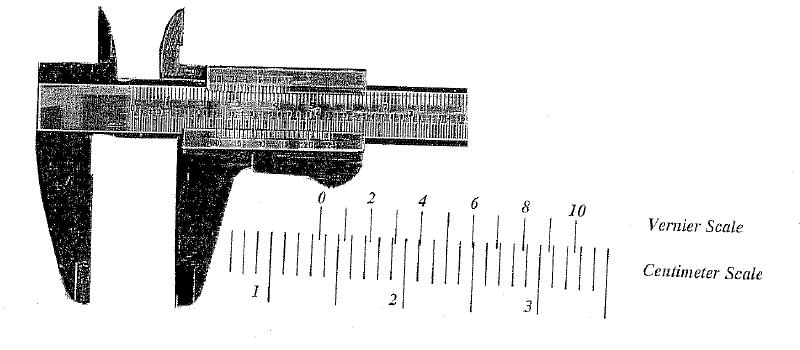
\includegraphics[width=6in]{vernier.JPG}
\vspace{-.25cm}
\caption{The Vernier Caliper:  The location of the zero on the vernier scale tells you where to read the centimeter scale (1.3 cm).  The vernier-scale line that lines up tells you the next digit (5).  This picture measures $1.35\pm 0.01 \unit{cm}$.}\label{f:vernier}
\end{center}
\begin{center}
\hspace{-2cm}
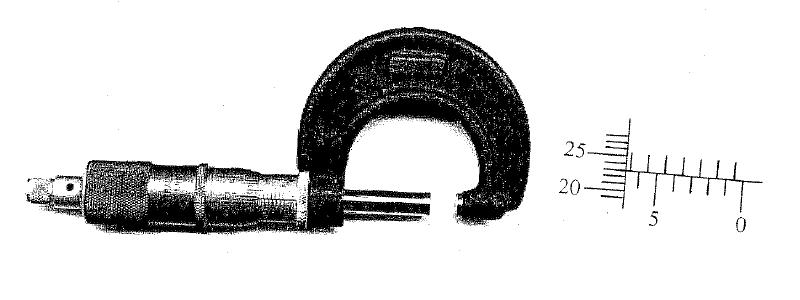
\includegraphics[width=6in]{micrometer.JPG}
\end{center}
\vspace{-.5cm}
\caption{The Micrometer Caliper:  Notice on the coarse scale, that the lower lines read (1, 2, 3, <ellipsis /> 6 in this picture) and the higher lines read the half-marks (0.5, 1.5, 2.5, <ellipsis /> 6.5 in this picture).  The location of the turning dial tells you where to read the coarse scale (6.5 mm).  The center line of the coarse scale tells you where to read the fine scale.  This is 23.0 (in units of $\times 10^{-2}$ mm), but not 23.5 and not 22.5 so the precision is 0.5 (in these units).  This measurement in mm reads $6.5 \unit{mm} + 0.230\unit{mm} = 6.730 \pm 0.005 \unit{mm}$. }\label{f:micrometer}
\vspace{-.5cm}
\end{figure}
%

%-------------------------------------------------------------------------------------
\onecolumn

\section{Standard Deviation}
\revised{Aug. 28, 2009}
\revision{Aug. 28, 2009}{Added Jack's picture back in}
\revision{Jan. 7, 1997}{Jack}

\subsection{Introduction}

Suppose you are standing in front of a dart-board.  You have a large number of darts and you throw the darts one at a time, trying to hit a 1 cm thick vertical line drawn on the dart-board.  Since you have a very good aim, let us say that 45\% of the darts hit the line.   This then means that you miss the line 55\% of the time; with a significant number of these misses being between .5 to 1.5 cm either to the left or to the right from the center of the line, and with a smaller number of misses being between 1.5 to 2.5 cm from the center line.

Is there some mathematical way of characterizing how good you are at this game?  What, for example, is the probability of missing the line by 1 cm?  The statistical analysis of random fluctuations in data can help answer these questions.   The word ``statistical'' implies that a relatively large set of similar measurements of a given physical quantity is available.  The random fluctuations in the data can be measured with the use of a mathematical term called the ``standard deviation.''

Suppose you collect data on a large number of throws, separating the data into categories (bins): The number of darts on the line, the number within .5 to 1.5 cm from the center, the number within 1.5 to 2.5 cm, etc.  A plot of this data with the dart positions on the x-axis and the number of darts hit within each bin plotted on the y-axis is called a histogram (see Figure~\ref{f:histogram}).  The envelope of this graphical data set is bell shaped, and is called a Gaussian or a Normal distribution curve.
%
\begin{figure}[bhtp]
\begin{center}
%\begin{picture}(400,200)
%\put(0,0){\line(0,1){200}}
%\put(0,0){\line(1,0){400}}
%\put(200,195){\vector(0,-1){25} $\mu$}
%\put(200,100){\vector(1,0){75}}
%\put(200,100){\vector(-1,0){75}}
%\put(200,105){$\sigma$}
%\end{picture}
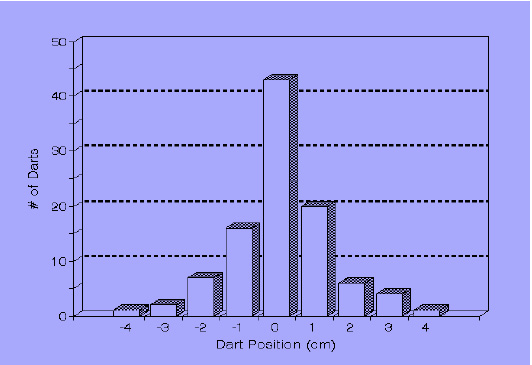
\includegraphics[height=2.5in]{darthistogram.jpg}
\caption{Histogram for the number of darts binned by distance from the centerline.}\label{f:histogram}
\end{center}
\end{figure}


The ``standard deviation'' is a measure of the spread or width of the histogram data.  A small standard deviation  means that there is a small spread in the data about the central mean value and implies that the data cluster closely about one value.   That is, there is a high degree of precision in the measurements.


The area beneath the curve, or below a part of the curve represents the probability of occurrence.  For example, the area beneath the curve between plus and minus one standard deviation from the mean represents a 68\% probability of your next throw falling within this range.  The area beneath the curve between plus and minus two standard deviations from the mean represents a 95\% probability of your next throw falling within this range.

In this experiment, you will study the use of the ``standard deviation'' in the statistical analysis and probability involved with flipping pennies.
\subsection{Experimental Purpose}

The goal of the experiment is to determine how the mean, standard deviation, and standard deviation of the mean depend on the amount of data (number of samples) taken.  You should also consider how well the data fit to a normal distribution.

\subsection{Student Outcome}

In this experiment, you should learn
\begin{enumerate}
\item the formulas for and the roles of the mean, the standard deviation, and the standard deviation of the mean in the statistical analysis of data containing random errors,
\item how to create histograms and scatter plots,
\item how to include trendlines on scatter plots, and
\item why more data is always better.
\end{enumerate}

\subsection{Pre-Lab Work}
\begin{lablist}
\item Define the following, both in a sentence and with a mathematical formula:  mean, standard deviation (sometimes called the standard deviation of a single observation), and standard deviation of the mean.  Be sure to describe the difference between these two terms.
\item Define the following:  histogram, probability, \& probability distribution (Normal distribution).
\item What does the total area under the Normal distribution curve represent?
\item How should the axes of the histogram of the data you will take for this lab be labeled?  Give a very specific scale for the x-axis.  (Hint: Read the procedure below.)
\item Make a sketch of an inverse function, like $y=1/x$.
\end{lablist}

%\twocolumn[\vspace{-.5cm}
\subsection{Experimental Procedure}

Each individual will receive 20 pennies and will then simultaneously toss all of the pennies.  Count the number of heads, and repeat 25 times.   Each individual will then have collected 25 pieces of data.
%\\]

\subsection{Analysis}

\begin{lablist}
\item Calculate the mean, the standard deviation  and the standard deviation of the mean for your first ten tosses and for all 25 tosses.  Show your calculations.
\item Make a histogram plot (by hand in your note book) for your 25 tosses.   On this histogram superimpose a sketch of your best guess of the corresponding Normal distribution curve.
\item How well does your data fit a normal distribution curve?  Explain the reasons for any large discrepancies.
\item Obtain histograms and calculations of the mean, the standard deviation and the standard deviation of the mean for the following data sets:  i) your lab group,  ii) about 1/2 of the class, and iii) the entire class.   These histograms can be obtained with the use of a computer program, provided by the instructor.
\item Draw graphs of:  the mean, the standard deviation, the standard deviation of the mean, versus the number of data entries.   Use the standard deviation of the mean  as the error bars for both the mean and the standard deviation,  draw these error bars on these two graphs.
\item Describe how the values of the mean, the standard deviation, and the standard deviation of the mean, change as the number of data items in the set increases.  What does this infer about the accuracy and about the precision of the data as more and more observations are made?
\item Show that the standard deviation of the mean varies inversely as the square root of the number of data items in the sample.   How well does the data in this lab agree with this prediction?   (Make a graph of the standard deviation of the mean versus the square root of the number of data items in the sample.)
\end{lablist}

\subsection{Questions}
\begin{enumerate}
\item What is the probability of flipping the 20 pennies and getting 5 heads, or 8 heads, or 10 heads, or 15 heads?   Answer this question by analyzing your data, the entire class' data and the normal distribution curve fit to your data.  Explain any differences between these sets.
\item What percentage of your individual readings fall within plus or minus one standard deviation,  two standard deviations?   Compare your answer to the theoretical answer from a normal distribution curve.  What are the percentages for the class data?
\item Does the height of the histograms change as a function of the number of trials?  If so, how?
\item How does the width at 1/2 the maximum height for the histograms change as a function of the number of trials?  Label this width on your histograms.  Is this width a reasonable estimate of the standard deviation?
\item Does the standard deviation of a single observation and/or does the standard deviation of the mean change significantly as the number of tosses increase?  What does this infer about the accuracy and about the precision of the data as more and more observations are made?
\end{enumerate}

\subsection*{Resource Materials}

Meyer, \underline{Data Analysis for Scientists and Engineers} John Wiley, (1975) p.19-48, 223-253


%-------------------------------------------------------------------------------------
\onecolumn

<chapter><title>Constant Acceleration</title>
<!-- Revisions
\revised{Sept. 14, 2015}
\revision{Sept. 14, 2015}{Commented out Graphs and Tracks.  Updated Pasco Reference from DataStudio to Capstone}
\revision{Sept. 16, 2008}{Created?}
-->

    <objectives><title>Experimental Purpose</title>
    <introduction><p>Using position versus time and velocity versus time graphs, verify that the equations of constant acceleration accurately describes the behavior of objects under constant acceleration and that it is possible to distinguish acceleration due to gravity from acceleration due to friction.</p>
    </introduction>
    </objectives>

    <section><title>Student Outcomes</title>
    <p>In this exercise, the student should develop an understanding of the relationships between the position and the instantaneous velocity of an object, as well as how each of these can vary as functions of time.   We will only consider the special case where the object experiences constant acceleration.</p>

    </section>

    <section><title>Materials</title>
    <p>An aluminum track, a low-friction cart, computer interface with PASCO Capstone<m>^{\rm tm}</m> software, a sonic motion sensor, a small steel ball.</p>
    </section>

    <section><title>Procedure (to be paired with Section~\ref{ss:AccAnalysis})</title>

    <subsection><title>Cart and Flat Track</title>\label{sss:FlatTrack}
    <p>Log into the computer (so you can save your data to your network drive) and then open Pasco Capstone.
    (Section~\ref{s:Capstone} will provide some instructions for setting up the software and connecting the equipment.)
Connect the motion sensor to the computer interface.
Set the data rate of the motion sensor at <m>50 \unit{Hz}</m>.
Place a steel ball on the track and adjust the leveling screw at one end of the track to see if the ball rolls one way or the other.  This will roughly level your track.
Place the sensor about 20 cm from the end of the track, because this is the minimum distance detected by the sensor.  (You might need to use the <q>sail</q> for the sensor to see the cart.)</p>

    <p>Place the cart on the track.  Capstone, via the sonic ranger, can measure the position and velocity of the cart as a function of time.  (This is explained in Section~\ref{s:Capstone}.)
<ol>
<li><p> Assume the track is frictionless and predict how the cart will move if the track is not perfectly level; include a comment about how the velocity versus time graph will look when it goes uphill versus when it goes downhill.  Should these be the same?
</p></li> <li><p> What do you expect the graph to look like if the track <em>is</em> perfectly level?  Will it be the same going left versus going right?
</p></li> <li><p> Now, assuming it is perfectly level, what will friction do to the motion?  How do you expect this to affect the graphs?
</p></li> </ol>
\setcounter{dave}{\theenumi}
</p>

    <p>We will take four sets of data: a slow, constant velocity towards the ranger; a slow, constant velocity away from the ranger; a faster, constant velocity towards the ranger; and a faster, constant velocity away from the ranger.  The two slow speeds should be about the same and the two faster speeds should be about the same.  For each case, start the sonic ranger and then bump the cart firmly, but not violently(!).</p>

    <p>On Capstone, you should have four curves of velocity versus time.  Fit each with a trendline and display the equation of the trendline on the screen.  Interpret the coefficients (slope and intercept) by noting their units, values, and uncertainties.  You should also print out (in landscape mode) the position versus time graph, the velocity versus time graph, and the acceleration versus time graph.  (You should notice that the acceleration versus time graph is <em>very</em> noisy.)</p>

    </subsection>
    <subsection><title>Cart and Sloped Track</title>\label{sss:SlopedTrack}
    <p>Place a small block under one end of the track, so that the track is now tilted at a small angle with the sensor at the top of the incline.  Measure the angle using a protractor or calculate it by measuring the two legs of the triangle and using the inverse sine.  (Be careful about measuring the height.)</p>

    <p.>We will consider <em>three cases</em> for the sloped track: <em>First</em>, allow the cart to roll (without an initial push) down the ramp.  <em>Second</em>, gently push the cart down the ramp.  DON'T let it fly off or crash into anything.
<ol>
\setcounter{enumi}{\thedave}
<li><p> Should these two cases have the same acceleration while rolling down the ramp?  How will that affect the shape of the velocity versus time graphs?
</p></li> <li><p> Should these have the same initial velocity?  How will that affect the graphs?
</p></li> </ol>
\setcounter{dave}{\theenumi}
In the <em>third</em> case, start the cart at the bottom of the incline and roll it up the ramp, allowing it to roll back down on its own.  Push it hard enough to get mostly up the ramp, but not so hard that it hits the sonic ranger.
<ol>
\setcounter{enumi}{\thedave}
<li><p> Should this case have the same acceleration while it goes up the ramp as while it goes down the ramp? How can we see that on the velocity versus time graphs?
</p></li> <li><p> Should this case have the same acceleration (either while it goes up the ramp or while it goes down the ramp) as the previous two cases of rolling down the ramp?
</p></li> </ol>
\setcounter{dave}{\theenumi}
</p>

    <p>In Capstone, you should be able to display all three graphs (position v time, velocity v time, and acceleration v time).  You should also be able to display all three cases of data on each of these graphs.  On the velocity versus time graph, fit each of the three graphs with a linear trendline.  The next section will ask you to analyze how well the data match up to these lines.  (It might be interesting to also fit the position vs time curves to parabolas.  Be sure to print out copies of your three graphs.</p>

    <p>Your lab should note the following results and explain their meaning:  slope and y-intercept, the uncertainties (precision) in both the slope and intercept, and the <m>r</m> value (correlation coefficient). </p>

    </subsection>
    </section>

    <section><title>Further Analysis and Discussion</title>\label{ss:AccAnalysis}

    <subsection><title>Cart and Flat Track</title>

    <p>Based on the results of Sec.~\ref{sss:FlatTrack}, write a short analysis of the relationship between these two graphs (x and v versus time).   From the velocity versus time graph (specifically from the trendline) determine the value of the acceleration of the cart down the track; be sure to include the uncertainty of the acceleration and the units.
<ol>
<li><p> Do you see any evidence that the track was not perfectly level?
</p></li> <li><p> Do you see any evidence that there is any friction as the cart moves along the track?
</p></li> <li><p> What does the intercept of the velocity versus time graph tell you?
</p></li> <li><p> If the slopes are different, then discuss any pattern that you see.  If the slopes are (essentially) the same, then find an average and a standard deviation of the four values.
</p></li> <li><p> Does it matter how fast the cart travels?
</p></li> </ol>
\setcounter{dave}{\theenumi}
    Discuss any evidence observed in your data when answering these questions.  Also consider the magnitude of the uncertainties when writing your conclusions.</p>

    </subsection>
    <subsection><title>Cart and Sloped Track</title>

    <p>Based on the results of Sec.~\ref{sss:SlopedTrack}, write an analysis of the relationship between the two graphs
(x and v versus time).  From the velocity versus time graph determine the value of the acceleration of the cart down the track.
<ol>
\setcounter{enumi}{\thedave}
<li><p> For the two downhill cases, use your uncertainty analysis to determine if the acceleration of the cart changed when it was given a small push.
%</p></li> <li><p> For the case that you copied into Excel, compare the results for the acceleration (with uncertainties) between <q>Data Studio</q> and Excel.  Comment on any differences.
</p></li> <li><p> Is there an accuracy<fn>If the track were frictionless, then the acceleration should be <m>a=(9.81\unitfrac{m}{s^2})(\sin\theta)</m>, where <m>\theta</m> is the angle that the incline makes.</fn> that can be computed for this part of the experiment?
</p></li> </ol>
\setcounter{dave}{\theenumi}
%
Inspect the line/curve that is defined by the data on the Distance traveled vs. time graph.
<ol>
\setcounter{enumi}{\thedave}
<li><p> What is its shape?  Is the shape of the graph what you would expect for constant acceleration (straight line, parabola, etc.)?  Explain your reasoning.
</p></li> <li><p> Consider the trendline that you added.  Does/should the trendline line go through the origin?  What is the value of y-intercept of the X vs T graph?  What physical quantity does the intercept represent?  Explain why it has that value.  Hint: (Think about where the sensor was located.)
</p></li> <li><p> What does the slope (whether it's constant or not) of the line on this graph signify?
</p></li> </ol>
\setcounter{dave}{\theenumi}
Now consider the Instantaneous Velocity  vs. Time graph.
<ol>
\setcounter{enumi}{\thedave}
<li><p> Does the curve/line on this graph have the shape you would expect for an object undergoing constant acceleration? Explain.
</p></li> <li><p> What was the value of the y intercept on this graph (include units and uncertainty!)?  Explain its significance.  To what does it refer?  Think carefully about what you plotted on the X-axis!
</p></li> </ol>
    </p>

    </subsection>
    </section>
</chapter>

%-------------------------------------------------------------------------------------
\onecolumn

<chapter><title>Newton's <m>2^{\rm nd}</m> Law on a Linear Track with the Sonic Ranger</title>\label{s:Newton}
<!-- Revisions
\revised{Sept. 14, 2015}
\revision{Sept. 14, 2015}{Updated Pasco Reference from DataStudio to Capstone}
\revision{Sept.~23, 2008}{}
-->

<introduction><title></title>Introduction to Forces}

Forces are related to the natural motion of bodies, where one object can affect the motion of another object.  That is, forces are interactions between objects affecting their motion.  Although the famous Greek philosopher Aristotle claimed that a force was necessary to <em>maintain</em> any motion, careful analysis by Italian physicist Galileo Galilei in the mid-<m>17^{\rm th}</m> century and by Sir Isaac Newton, a British mathematician and physicist (1642-1727), eventually distinguished the effects of friction and allowed Newton to create a mathematically consistent theory of motion.  These concepts were published in Newton's book <q>Mathematical Principles of Natural Philosophy</q> in 1687, for which (among other accomplishments) Newton is regarded as one of the greatest scientists of all time.

All forces can be placed in one of two main categories.  First, there are natural (or fundamental) forces like the gravitational force, the electromagnetic force, or the nuclear forces.  The gravitational force is a force on a body by another body (like the Earth), this force is an interaction between their two masses.  The electromagnetic force is an interaction between the charges of two bodies.  These forces may act on an object without any direct physical contact between the two bodies.  This type of force is sometimes called an <q>action at a distance</q> force.  All other forces are in a second category called <q>contact forces.</q>

<subsection><title></title>Newton's First law}

<quote>
If there are no forces acting, then objects will remain at rest or, if not at rest, will maintain their velocity.
</quote>
If this is true, then we can study the forces acting on a body based on the motion of the body, specifically through the change in the velocity of an object.

</subsection>
<subsection><title></title>Newton's Second Law}

Not only is a force necessary to change the motion (to cause an acceleration), the amount of acceleration that a force causes is predictable and is inversely proportional to the mass.  The same sized force causes a small mass to accelerate a lot and a large mass to accelerate a little.  this is expressed by the equation:
<me> \vec F_{\rm net} = m \vec a. </me>
The net force, <m>\vec F_{\rm net}</m>, is the vector sum of all forces acting on an object.  If we have an extended object (such as a weight hanging off of a table, but connected to a cart that is on the table), then we need only consider forces that are <q>external</q> to the system:  So long as both objects accelerate at the same rate, we do not need to consider the <q>internal</q> tension that the string exerts between the connected bodies.

</subsection>
<subsection><title></title>Newton's Third Law}

Inherent in the description of a force is that it is an interaction between objects: there must always be two objects that interact.  These objects exert equal and opposite forces on each other.  That is,
<quote>
If there is a force exerted on object 1 by object 2, then there is necessarily and simultaneously a force exerted on object 2 by object 1 that is equal (in magnitude) and opposite (in direction) to the original force.
</quote>
Remember that these two forces are on different objects and that the two bodies in direct contact exert forces on each other.  Remember then that if there is contact between the object (any part of the system) and anything else then there is an outside force on the object (system) and that if there is no contact (the two bodies break contact) then there is no force.


</subsection>
</introduction>
    <objectives><title>Experimental Objective</title>

    <introduction><p>In this experiment, we will assume that the first law is true and focus on the second law.
    By measuring (a) the velocity versus time for a cart being pulled down a track and (b) the applied force that is pulling it, we can plot the acceleration versus the force and verify the validity of Newton's second law of motion: <m>\vec F_{\rm net} = m \vec a</m>.</p>
    </introduction>
    </objectives>

</section><section><title></title>The Experimental Setup}

<ul>
<li><p> A low-friction linear cart and track will be used, this reduces the friction between the cart and the track.
</p></li> <li><p> A string will be connected to the cart and a known mass will be hanging from the end of the string (and over a pulley).   The hanging mass will exert a constant horizontal force on the cart as the mass falls all the way to the floor.  This gives a constant acceleration to the cart.
</p></li> <li><p> The sonic motion sensor will be used to measure the position of the cart as a function of time.
</p></li> <li><p> The carts and tracks need to be handled with care.  Scratches can add friction to the system.
</p></li> </ul>

</section><section><title></title>Pre-Lab Work}

<ul>
<li><p> Draw a free-body force diagram for the cart and for the hanging mass.
</p></li> <li><p> Derive an equation for the acceleration of the system, in terms of, the mass of the cart and the hanging body.
</p></li> </ul>

</section><section><title></title>Procedure}

<ul>
<li><p> If the cart is given an initial push (without the hanging mass and string attached) then the cart should travel with a constant velocity down the horizontal track, if there are no other forces acting on the cart.  Carry out  a couple of constant velocity runs on the track, to check for the effects of friction and to see how level the track is. The track may need a level adjustment.  Do runs in both directions.  Maybe the track can be tilted so that the friction is countered by the tilt of the track.
</p></li> <li><p> Connect a string to the cart and run it through the hole at the end of the track, then over a pulley.  Make sure that the string is horizontal.  Measure the height of the string at both ends of the track, to see if the string is horizontal.
</p></li> <li><p> The hanging mass should be much less than the mass of the cart.  Use a small plastic cup to hold the hanging masses.   Measure the mass of  this cup.  The total mass of the system must be kept constant for all parts of the experiment.   The hanging mass and the mass of the cart should vary, but their total must be kept constant, by moving small mass amounts from the cart to the hanging cup.  Record the mass of the cart, the hanging cup mass, and the extra masses which are to be transferred from the cart to the cup.
</p></li> <li><p> Take data with Capstone and the motion sensor as the cart travels with constant acceleration down the track.   Determine the acceleration of the cart from a linear regression using the velocity vs time data (a linear fit line in Capstone).  Record the acceleration value and its uncertainty.
</p></li> <li><p> Collect  7 data runs, where about 5 grams is transferred each time from the cart to the hanging mass.   Determine the acceleration of the cart (and the uncertainty for the acceleration) for each of these 7 runs.
</p></li> </ul>

</section><section><title></title>Analysis}

<ul>
<li><p> Make a graph of the acceleration of the system (y-axis) versus the weight (<m>mg</m>) of the hanging body (x-axis),  should include 7 data points.    Do this in Excel.   Carry out a linear regression for this data set.   Quote the  slope and intercept values, their uncertainties, their p-values, and the <m>R^2</m> value.     Show a sample error bar (on the graph) for at least one of the points of this graph.
</p></li> <li><p> Derive (show it completely)  an equation for the acceleration of the system versus the weight of the hanging body.  Plot this theory equation on your graph (as a second series, a line but no points).
</p></li> <li><p> Compare your graph to the predicted theoretical equation, that is compare the values of the slopes and intercepts.  What is the physical significance of the slope and of the intercept from the graph?  That is, what physical quantity does the slope of this graph equal?
</p></li> <li><p> In many mechanics experiments, there may be deviations from the expected or theoretical results because of the effects of friction.  Frictional forces are sometimes difficult to take into consideration.  If there are deviations between your results and the predicted theory then try to distinguish whether they are caused by a tilt of the track, friction between the cart and the track or the friction between the string and the pulley.  What might be expected in the results from these different systematic effects?    That is, would the slope be expected to increase or decrease slightly because of the effects of friction?
</p></li> <li><p> When designing experiments, it is important to keep control parameters; in this case a parameter which is kept constant.   What parameter held this role in this experiment?
</p></li></ul>

%\vfill\hfill(<m>\hookrightarrow</m>)
%\onecolumn
</section><section><title></title>Questions}

<ol>
<li><p> Why is it important to keep the total mass of the system constant?   What would happen if the total mass of the system was not held constant?    If one simply added mass to the hanger without keeping the system's mass constant,  how would their data appear on the graph of the acceleration vs <m>mg</m>?
</p></li> <li><p> What would happen if the track was not level?   If the beginning end of the track is higher,  how would the acceleration of the system be affected?
</p></li> <li><p> If your group has a discrepancy between the results and the theory, could friction be used to explain your results?   Explain how.   In this case, how much of a tilt in the air track would be needed to explain the discrepancy?   Show this calculation.
</p></li> <li><p> What would happen to the cart's acceleration if the cart was given an initial push?
</p></li> <li><p> What are the two greatest sources of uncertainty in this experiment?   Are they random or systematic errors?   Be specific and quantify your answer.
</p></li> </ol>


</chapter>

%-------------------------------------------------------------------------------------
\onecolumn

<chapter><title>Dry Sliding Friction</title>
<!-- Revisions
\revised{Sept.~28, 2015}
\revision{Sept.~28, 2015}{}
\revision{Sept.~23, 2008}{}
-->

<introduction><title></title>Introduction}

Friction is a force which retards the relative motion of any body while sliding over another body.  The frictional force acting on a body is parallel to the surface that the object is sliding upon and it is directed opposite to the direction of motion.  The phenomenon of friction is rather complicated, especially at the microscopic level, because it is dependent on the nature of the materials of both contacting surfaces.  The frictional force depends on the roughness or the irregularities of both surfaces.  At the macroscopic level, the nature of this force can be described by a simple empirical law, first given by Leonardo da Vinci:
<quote>
The magnitude of the force of friction between unlubricated, dry surfaces sliding one over the other is proportional to the normal force pressing the surfaces together and is independent of the (macroscopic) area of contact and of the relative speed.
</quote>
At the microscopic level, the frictional force <m>(F_f)</m> does depend on the actual area of contact of the irregularities of the surfaces.  This actual area of contact then increases as the force pressing the two surfaces together increases, this force is called the load.  Using Newton's <m>2^{\rm nd}</m> Law in this perpendicular direction we can conclude that the magnitude of the load is equal to the Normal force <m>(F_N)</m> of the surface pushing on the object.  Therefore we may write that
%
<me>
F_f \propto F_N
\mbox{\ \ \ \ or \ \ \ \ }
F_f = \mu F_N
</me>
%
where the Greek letter <m>\mu</m> (<q>mew</q>) is a dimensionless constant of proportionality called the coefficient of friction.

When a body is pushed or pulled parallel to the surface of contact and no motion occurs, we can conclude that the force of the push or pull is equal to the frictional force, using Newton's <m>2^{\rm nd}</m> Law of motion.  As the applied force is increased, the frictional force remains equal to the applied force until motion results.  At this maximum value of the applied force, the frictional force is also a maximum and is given by
%
<me>
F_f = \mu_s F_N
</me>
%
where the subscript <m>s</m> stands for static (non-moving) friction.  This equation can only be used at this maximum static point also called the point of impending motion.  At the instant that the applied force becomes greater than the maximum fs, the body is set into motion and this motion is opposed by a frictional force called the kinetic (sliding) frictional force and is given by
%
<me>
F_f = \mu_k F_N
</me>
%
where the subscript <m>k</m> stands for the kinetic (moving) friction.  In general, <m>\mu_k < \mu_s</m>; that is, it takes more force to overcome the static friction than to over come the kinetic friction.  The coefficients of friction are generally less than one, but may be greater than one, and they depend on the nature of both surfaces.



	Consider a system comprised of a block on a horizontal surface being pulled horizontally by a string connected to a hanging weight.   Assume that the system is accelerating with a constant acceleration.  Then the <m>\mu_k</m> can be solved for by the following equation:
%
<me>
\mu_k  = \frac{ mg - (M+m) a }{ Mg},
</me>
where <m>M</m> is the mass of the block and <m>m</m> is the hanging mass.


    </introduction>
    <objectives><title>Experimental Objective</title>

    <introduction><p>In this experiment you will devise methods to investigate the nature of both the frictional force and the coefficient of friction, and to test the validity of da Vinci's empirical rule.</p>
    </introduction>
    </objectives>

<section><title></title>Pre-Lab Analysis}

<ul>
<li><p> Draw force diagrams for the following case:     a block on a horizontal surface pulled by a hanging mass and a string  (include the friction force).
</p></li> <li><p> Write out the corresponding Newton's <m>2^{\rm nd}</m> Law equations for forces both parallel and perpendicular to the contact surface.
</p></li> <li><p> Derive the relevant equations for each of the above two cases for which the coefficients of friction can be determined:
    <ul>
    <li><p> Case one is static, but at the point of motion.
    </p></li> <li><p> Case two is the kinetic case.
    </p></li> </ul>
</p></li> </ul>


</section><section><title></title>The Experiment}

For the block on the horizontal plane:	
<ol>
<li><p> Clean the block and the plane, so that they are free of dust and other contaminants.  \\
Make sure the track is level, as in previous labs.
</p></li> </ol>
\setcounter{dave}{\theenumi}

</subsection><subsection><title></title>Break Static Friction - pull until moves}\label{sss:staticfriction}
<ol>
\setcounter{enumi}{\thedave}
<li><p> Set up the Dynamics Track, cart, force transducer and friction block.  The force transducer attaches to the dynamics cart, the friction block rests on the track (felt side down).
</p></li> <li><p>\label{i:staticpull} Attach a string to the force transducer.  The force transducer needs to be zeroed before data collection starts.  Collect data, and slowly start pulling on the string (<em>be sure to pull the string horizontally</em>) and slowly increase the pull force until the cart is moving down the track. Using just the maximum force (at the point of impending motion) the coefficient of static friction can be calculated.
</p></li> <li><p>\label{i:statictest} Test the relationship between the force of friction and the normal force, by changing the load force (normal force) and measuring the force of friction at the point of motion impending. Carry this out for a total of five data points.  Graph the frictional force versus the normal force.  Calculate the coefficient of static friction from this graph.
</p></li> </ol>
\setcounter{dave}{\theenumi}

</subsection><subsection><title></title>Effect of Surface Area - distinguish pressure from force}\label{sss:friction-area}

Consider pushing a pencil into your arm. (Well, don't <em>actually</em> do it!)  If you use the erasure end, then you can feel the force, but it doesn't hurt.  If you use the sharpened tip with the <em>same</em> force then it will certainly hurt!  So, you have the idea that the same force spread over a different surface area <em>can</em> have a different effect; but it doesn't <em>always</em> have a different effect.  For this part of the lab, you will test the relationship between the coefficient of friction and the macroscopic area of contact between the block and the surface.
<ol>
\setcounter{enumi}{\thedave}
<li><p> Place the friction block on its side (felt side down) and repeat Steps~\ref{i:staticpull} and~\ref{i:statictest} for three (rather than five) of the previous load forces.
</p></li> <li><p> Add the plot of this <m>F_f</m> versus <m>F_N</m> as a new series to the graph of Part~\ref{sss:staticfriction}.
</p></li> </ol>
\setcounter{dave}{\theenumi}

</subsection><subsection><title></title>Friction while Accelerating}

<ol>
\setcounter{enumi}{\thedave}
<li><p> Apply a force (hanging mass, pulley, and string) large enough to accelerate the block. Use the Sonic Ranger to collect data.
</p></li> <li><p> Graph the velocity vs time.  Determine the acceleration of the block from the slope of the line.
</p></li> <li><p> Repeat this part four or five times with a different normal forces.  (You may use any hanging mass.)
</p></li> <li><p> Add the plot of this <m>F_f</m> versus <m>F_N</m> as a new series to the graph of Parts~\ref{sss:staticfriction} and~\ref{sss:friction-area}.
</p></li> <li><p> Calculate the coefficient of kinetic friction from the slope.
</p></li> </ol>



</section><section><title></title>Analysis}
<ul>
<li><p> The experimental precision should be estimated for all parts of this experiment and care should be taken for all of the measurements, but it is more important to investigate the relationships than it is to repeat the experiment many times or to try to achieve high precision in the data.
</p></li> <li><p> Explain why the normal force on the block by the surface rather than the weight of the object is related to the frictional force.
</p></li> <li><p> Interpret the slope and intercept of the graphs.
</p></li> <li><p> Compare the slopes from each of the three parts.  Decide which should be the same and which should be different.
</p></li> <li><p> Calculate the \% decrease of the static to kinetic coefficient of friction.
</p></li> <li><p> Comment on the validity of the empirical rules of friction.
</p></li> </ul>


</section><section><title></title>Questions}

For all questions, and when possible, use your experimental or theoretical results to demonstrate your answers to the questions.
<ol>
<li><p> Does the coefficient of friction depend on the area of contact?
</p></li> <li><p> Does the coefficient of friction depend on the mass of the object?
</p></li> <li><p> Does the coefficient of friction depend on the normal force of the object?
</p></li> <li><p> Does the frictional force depend on the normal force of the object?
</p></li> <li><p> Does the coefficient of kinetic friction depend on the speed of travel?
</p></li> <li><p> When the object was pulled by a string, how would the forces be affected if the cord was not horizontal?
</p></li> <li><p> What would happen to the coefficient of friction if the surfaces were lubricated with oil?
</p></li> </ol>


</chapter>

%-------------------------------------------------------------------------------------


\onecolumn
<chapter><title>Centripetal Force</title>
<!-- Revisions
\revised{Fall 2006}
-->
<introduction><title></title>Introduction}

We will be investigating the force which is necessary to maintain the circular
motion of an object.
The apparatus used will allow you to spin an F-shaped arm which has a mass
suspended from the
top arm.  This mass will be held in place by a spring which makes up the lower
arm.  The spring
will provide the centripetal force.  You will need to be familiar with the
ideas of circular motion,
centripetal versus centrifugal force, centripetal acceleration, and angular
velocity.  In addition to
these concepts, try to understand how we will measure the angular speed in lab.

The centripetal acceleration <m>a_c</m> is calculated from the following equation
written either <m>\displaystyle a_c=\frac{v^2}{r}</m> or <m>\displaystyle a_c =
\omega^2 r</m>
where <m>v</m> is the linear velocity of the particle, <m>\omega</m> is the
angular velocity, and <m>r</m> is the radius of the circle.  Note that angular
velocity is measured in radians per second.

From Newton's second law, <m>\vec F = m \vec a</m>.
Therefore, the force required to keep the particle of mass <m>m</m> moving in a
circle
with constant speed is
%
<me> F = ma_c = \frac{mv^2}{r} = m\omega^2r </me>
%
Recall that the centripetal force is not a force applied <em>in addition</em> to
other existing forces.
The centripetal force is <em>whatever combination</em> of existing force act to
maintain circular motion.

    </introduction>
    <objectives><title>Purpose</title>

    <p>It is our purpose to verify the above equation experimentally by measuring the applied force
and comparing it to the specific combination of variables expressed as either
<m>\frac{mv^2}{r}</m> or <m>m\omega^2r</m>.</p>
    </introduction>
    </objectives>

<section><title></title>Pre-Lab}

<ol>
<li><p> Why do we say that an object moving with <em>constant speed</em> in a
circular path is being accelerated?
</p></li> <li><p> In which direction is that acceleration?  How do you know?
</p></li> <li><p> Is this <m>a_c</m> <q>centripetal</q> or <q>centrifugal?</q>
</p></li> </ol>

</section><section><title></title>The Experiment}

The centripetal force is supplied by a spring.  Since we cannot directly
measure <q>the
force exerted by the spring while it is rotating</q> while it is rotating,
determine how
we can measure <q>the force exerted by the spring during the
rotation</q>
when the spring is not rotating.

<ul>
<li><p>\label{i:r} By means of the lab apparatus, a mass <m>m</m> can be made to rotate with a constant (and measurable) angular speed <m>\omega</m>.  With some practice, it is possible to adjust the speed so that the radius of the path remains constant.  The value of the radius, <m>r</m>, is marked on the apparatus and so can be measured easily.
</p></li> <li><p>\label{i:m} Measuring the mass should be an obvious task.
</p></li> <li><p>\label{i:w} Measuring the angular speed <m>\omega</m> is straightforward, but may not be obvious.  To do so, consider the following:
    <ul>
    <li><p> Angular speed <m>(\omega)</m> is measured in <m>^{\rm radians}\!\!/_{\!\rm second}</m>.
    </p></li> <li><p> <m>\omega</m> is related to the rotational speed which is measured in <m>^{\rm revolutions}\!\!/_{\!\rm second}</m>.
    </p></li> <li><p> There are <m>2\pi</m> radians in 1 revolution.
    </p></li> <li><p> We can count the number of revolutions.
    </p></li> <li><p> The <q>period of rotation,</q> <m>T</m>, is defined as the number of seconds per revolution.
    </p></li> <li><p> We measure the period not by timing a single revolution, but by measuring the time for multiple (20) revolutions divided by the number of revolutions. (This averages out any uncertainty due to reaction-time.)
    </p></li> </ul>
</p></li> <li><p>[] As the mass rotates, its period of rotation can be measured.  This allows you to calculate the angular speed using the hints above.
</p></li> <li><p> Repeat the entire procedure for a second value of r.
</p></li> </ul>

</section><section><title></title>Analysis}

From measurements of <m>m</m>, <m>\omega</m>, and <m>r</m>, calculate the theoretical centripetal force on
the mass (which experimentally is supplied by the spring).  The (unmeasurable) amount
of force exerted by the spring to hold the spinning mass at a particular radius is
equal to the (measurable) force required to stretch the spring to that radius.  Experimentally determine
the force necessary to stretch the spring to a specific radius and compare that with the amount
of centripetal force calculated above.
</chapter>

%-------------------------------------------------------------------------------------

\newpage

<chapter><title>Conservation of Energy on a Linear Track</title>
<!-- Revisions
\revised{October 24, 2015}
\revision{October 24, 2015}{made it a one week lab}
\revision{August 24, 2009}{}
-->

<introduction><title>Introduction</title>

Conservation laws play a very important role in our understanding of our physical world.  For example, the law of conservation of energy can be applied in all physical processes.  This is a fundamental and independent statement about the nature of the physical world.  It is not necessarily derivable from other laws like Newton's Laws of motion.  Though for simple point mass systems, the law of conservation of energy can be derived from Newton's Laws.  It can be shown that the net work done on a system is equal to the change in the kinetic energy <m>(W_{\rm net} = \Delta K)</m> of the system; this is called the work-energy theorem and it can be written in a variety of forms.  When a net positive work is done on a system, the kinetic energy of the system increases, and when a net negative work is done on the system (as from a friction force), the kinetic energy of the system decreases.

When the gravitational force acts on a system, the work it does on the system, <m>W_g</m>, is the gravitational force <m>(mg)</m> times the vertical displacement <m>(h=\Delta y)</m>: <m>W_g=mg\Delta y</m>.  For convenience, this is called the change in gravitational potential energy <m>(W_g = - \Delta P)</m>.  <em>If</em> the gravitational force is the only force acting on the system then <m>W_g = W_{\rm net}</m> and therefore, <m>-\Delta P = \Delta K</m> for the system.  When a force can be associated with a potential energy, it is called a <q>conservative force.</q>  Another kind of potential energy deals with an elastic potential energy, like in a spring.  The energy stored in a spring is given by the formula <m>P_s = \frac{1}{2} k \Delta x^2</m>.

<em>If</em>, on the other hand, a force dissipates energy, then it is called a <q>nonconservative force</q> and it will have no associated potential energy.  Frictional forces are an example of a nonconservative force and the work done by a frictional force is negative because (physically) the frictional force removes energy from the system and (mathematically) the frictional force and the displacement are in opposite directions.  This work done by friction is converted into heat or sound.  To distinguish the energy of heat or sound from the potential and kinetic energy, we define the total mechanical energy, <m>E=K+P</m> at any point.  Since frictional forces remove mechanical energy, we say <m>W_f = \Delta E = \Delta K + \Delta P</m>.

In general then, the law of conservation of energy states that energy can not be created or destroyed, but can only change from one form to another; or the total energy of the system at point A is equal to the total energy of the system at point B.

    </introduction>
    <objectives><title>Experimental Objective</title>

    <introduction><p>The purpose of this experiment will be to verify the validity of the law of conservation of mechanical energy, that <m>\Delta E = 0</m> as a cart runs along a track.</p>
    </introduction>
    </objectives>

</section><section><title></title>The Experiment}

We would like for you to verify the conservation of mechanical energy in two different situations; so, there are two parts to this experiment.
We will first consider a flat track with accelerated motion, as in the Newton's Law lab and the Friction lab.  We can then consider an inclined plane.  You will not be given an explicit procedure, but rather you will be given a series of questions with answers that will imply the procedure.  Part of the experiment is for you to figure out for yourself what the best course of action is.  Please answer the questions as they are asked.

%There is enough analysis for this lab that you will have two weeks to complete the lab.  During the first week, you will do the two parts of the experiment and begin to write up your report.  During the second week, you will do some analysis and re-run the experiment to determine the cause of differences from expectations.  A single lab report will be due after the second week of experimentation.

</subsection><subsection><title></title>Flat Track}\label{sss:1flat}

Set up the dynamics cart on a horizontal dynamics track.  Set up the motion sensor at one end of the track and a pulley at the other end so that the pulley partly extends past the edge of the table.  Hang the basket over the pulley so that it can accelerate the cart along the track -- you might need extra weight in the cart to keep it from accelerating too fast.  In order to use this motion to verify the validity of the conservation of mechanical energy, we need to measure some variables.  Answer Questions~\ref{q:1KE} and~\ref{q:1PE} to decide on the relevant variables.  Question~\ref{q1:2or1} should help you determine how to finish setting up the equipment.

Once you decide what variables to measure, run the experiment for one set of masses while measuring the appropriate variables.  Put the data into Excel and decide what plot(s) will allow you to verify the validity of the conservation of mechanical energy.  Question~\ref{q:1plots} may help with this.  Decide if you need a trendline.  Relate the information in Question~\ref{q:1EKP} to the statement you are trying to verify.

%Save your data so that you can do further analysis next week.

</subsection><subsection><title></title>Sloped Track}\label{sss:1sloped}

Remove the pulley from the track.  Your cart will have either a spring-loaded <q>battering ram</q> on the front or a pair of magnets.  If you have the battering ram, then you will want the end of the track with the rubber nub at the bottom of the incline.  If you have the magnets, then you need to replace the pulley with a <q>C</q> shaped <q>catch-bar.</q>  <em>Ask for help from the instructor!</em>  The catch-bar has magnets in it that will repel the magnets in the cart.  In this case, the cart must not be going so fast as to come into physical contact with the magnets on the catch-bar.

Raise one end of the dynamics track.  Question~\ref{q:1slope} should help decide how tilted.  Measure the tilt angle of the track with two methods: use a protractor, and measure the vertical rise and track length and calculate the tilt angle using the inverse-sine function.  Answer Question~\ref{q:1anglemeasurement}.  As you continue to set up the track for measurements, consider answering Questions~\ref{q:1KE}, \ref{q:1PE}, and~\ref{q1:2or1} again for this situation to help you decide on the appropriate accessories (sensors); but note Question~\ref{q:1rampangle} as you think about the answers to the previous questions.

Once you decide on the variables to be measured, but before you make the measurements, you will need to calibrate your position measurements.  We would like zero to correspond to being at the bottom of the ramp, so place the cart stationary at the bottom and use the motion sensor to measure this position.  In order to verify the validity of the conservation of mechanical energy, release the cart from rest near the top of the ramp and let it roll down the incline, bouncing three times before you stop the measurement.  Do this for one value of mass.
%Answer Question~\ref{q1:mass}.

Transfer these data to Excel again and decide on the best graph to verify the objective.  Again, Question~\ref{q:1plots} may help with this; however, you will also need to consider Question~\ref{q:1bounce}.  Decide if you need a trendline and where it would be fit.  Relate the information in Question~\ref{q:1EKP} to the statement you are trying to verify.

%\newpage
</section><section><title></title>Additional Analysis}% -- Considerations during the second week}

%For the second week, you should already have your graphs from the experiment and you should have written a significant portion of the theory and the analysis.
We are now going to take a closer look at the irregularities of the data and investigate some variations to try to explain what those data say.

<ul>
%</p></li> <li><p> One of the factors you were asked to consider last week was Question~\ref{q1:mass}.  In order to verify this, re-run Part~\ref{sss:1flat} with a noticeably different massed cart.  Re-create the graph and use this only to note the effect of a different mass.  Answer Question~\ref{q1:mass2}.

<li><p> Before drawing conclusions about the validity of the conservation of mechanical energy, consider Question~\ref{q:1missing}.

%</p></li> <li><p> As you evaluate Part~\ref{sss:1sloped}, you might be asked to re-run the experiment with a force transducer placed at the bottom of the track.  (This should imply where the motion sensor will go.) Make sure that the cart will bounce from the force sensor. Make sure that the force sensor is zeroed before the start.  There might be some information here based on work as a force-through-a-distance versus work as a change-in-energy.

</p></li> <li><p> One explanation of a loss of energy (non-conservation) is friction.  List all of the places where two pieces of material rub against each other.  Since <m>F_f = \mu F_N</m>, do any of these locations have a normal force that can be varied?
    %(Recall Questions~\ref{q1:mass} and~\ref{q1:mass2}.)
    (Recall Question~\ref{q1:mass2}.)
    As an independent measure of the amount of friction, we can also consider the actual acceleration versus the expected acceleration.  Question~\ref{q:1accel} will help you determine the expected acceleration and the variable necessary to find it.  Question~\ref{q:1fracc} will help decide on the relationship between the friction and the acceleration.

</p></li> <li><p> A second explanation for the loss of energy is that some component is gaining rotational kinetic energy.  The formula for this is <m>K_R = \frac{1}{2} I \omega^2</m>, where <m>I</m> is the moment of inertia<fn>In this case, the moment of inertia is probably a little less than <m>\frac{1}{2} m r^2</m>, where <m>m</m> is the mass of the rotating object and <m>r</m> is the radius of the rotating object.  This is not a convenient way to calculate <m>I</m> at this time.</fn>, and <m>\omega</m> is the angular speed <m>\omega = v/r</m>.  Assuming that any discrepancy that you found in the conservation of energy is due to the rotational kinetic energy of the pulley, how much energy would the pulley need to have at the end of the run (while spinning full speed)?  Based on the final velocity of the cart, what is the angular speed of the pulley?  Based on these numbers, <m>K_R</m> and <m>\omega</m>, what is the moment of inertia for the pulley?   Can you tell if this is a reasonable estimate?
</p></li> </ul>


%\newpage
</section><section><title></title>Questions}

    <ol>
    <li><p>\label{q:1KE} In order to verify <m>\Delta E=0</m>, we will need to calculate <m>E</m> as <m>E=K+P</m>. Therefore, we need to know the kinetic energy, <m>K=\frac{1}{2} m v^2</m>, the energy of <em>some mass</em>, <m>m</m>, moving at a speed <m>v</m>.  Which mass do you need to measure?  How can you measure the velocity?
    </p></li> <li><p>\label{q:1PE} In order to verify <m>\Delta E=0</m>, we will need to calculate <m>E</m> as <m>E=K+P</m>. Therefore, we need to know the potential energy, <m>P=m g y</m>, the energy of <em>some mass</em>, <m>m</m>, located some height, <m>y</m>, above the ground.  Which mass do you need to measure?  How can you measure the position?
    </p></li> <li><p>\label{q1:2or1} In order to measure the position of the falling mass and the velocity of the system, do you need two motion sensors?  Can you manage with one?  Considering that it is a fairly expensive piece of equipment, where should you NOT put the sonic ranger?  Where could you put it?  Depending on where you put the ranger, decide if you need to <q>translate</q> the position or velocity data in order to find the specific values that you actually need.
    </p></li> <li><p>\label{q:1plots} To verify <m>\Delta E=0</m>, we will need to graph <m>E</m>, the total mechanical energy, as a function of time.  What do you expect this graph to look like, if the law is valid?  If not?
        <ol>
        <li><p> Does the kinetic energy change during this motion?  Is <m>\Delta K=0</m>?  Considering the initial and final values of the kinetic energy, <m>K_i</m> and <m>K_f</m>, what would a graph of <m>K</m> versus time look like?
        </p></li> <li><p> Does the potential energy change during this motion?  Is <m>\Delta P=0</m>?  Considering the initial and final values of the potential energy, <m>P_i</m> and <m>P_f</m>, what would a graph of <m>P</m> versus time look like?
        </p></li> <li><p> Assuming that the mechanical energy is conserved, what would a graph look like if it included <m>E</m>, <m>K</m>, and <m>P</m>?  What if the mechanical energy is not conserved?  How would <m>K</m> and <m>P</m> be affected in these two cases?
        </p></li> <li><p>\label{q:1bounce} (Part~\ref{sss:1sloped} only) When the cart is at the bottom of the track during the motion, the values of position become negative (less than zero!).  Why?  Is there some other place where the energy might go?  %If you are using the force transducer, then it has a spring and a spring potential energy, <m>\Delta P_{\rm spring}</m>.  This can (and should!) also be included in the total mechanical energy.  You can calculate the elastic potential energy stored in the spring of the force transducer with <m>P = \frac{1}{2} k \Delta x^2</m>, which, since we do not know <m>k</m>, can be written <m>P = \frac{1}{2} F \Delta x</m>, where F is the force in Newtons (measurable with the force transducer) and <m>\Delta x</m> is the distance from the spring's equilibrium position, not the height (derivable from the position data).  Be sure to match up the force values and the <m>x</m> values at those same times.
        </p></li> </ol>
    </p></li> <li><p>\label{q:1EKP} Please note the overall change in potential energy, <m>\Delta P</m>, and the overall change in the kinetic energy, <m>\Delta K</m>.  Should either of these be related to the overall change in energy <m>\Delta E</m> and, if so, how?
    </p></li> <li><p>\label{q:1slope}  We want the cart to accelerate down the track (not too slow), but not to fly off at the bottom (not too fast).  How fast is <em>too fast</em>?  Don't use that slope!  How fast is <em>too slow</em>?  Use a slope somewhere in between.
    </p></li> <li><p>\label{q:1anglemeasurement}  After you measure the angle of incline in these two ways, consider the uncertainty in the measurements.  Which of these measurement is more precise?
    </p></li> <li><p>\label{q:1rampangle}  The motion sensor will measure the motion of the cart <em>along</em> the ramp, but the potential energy needs the <em>vertical</em> position of the cart.  Which trig function relates the distance along the ramp to the corresponding vertical distance?
    %</p></li> <li><p>\label{q1:mass}  Does the mass of the cart matter?  If you run it again at a different value of mass, would you expect the overall conclusion to be different?  Would you expect the specific values to be different?
    </p></li> <li><p>\label{q1:mass2} If the mechanical energy is conserved, then
        <me> \frac{1}{2} m v_i^2 + m g y_i = \frac{1}{2} m v_f^2 + m g y_f </me>
        What do you notice about the mass?  Is your graph different if the mass of the cart changes?  Does this support or conflict with the idea that the total mechanical energy is conserved?  On the other hand, if the mechanical energy is not conserved, then
        <me> W_{\rm nc} = \frac{1}{2} m v_f^2 + m g y_f - \frac{1}{2} m v_i^2 - m g y_i</me>
        What do you notice about the mass now?  Does your graph support or conflict with the idea that the total mechanical energy is conserved?
    </p></li> <li><p>\label{q:1missing} We need to look for the energy lost in each graph.
        <ol>
        <li><p> When you look at the graph from Part~\ref{sss:1flat} for <m>E</m>, is the energy conserved or is there energy lost?   If lost, calculate the energy lost or gained from the graph. (It might help to have a trendline.)  If energy is lost, come up with at least two explanations for where this energy goes.
        </p></li> <li><p> When you look at the graph from Part~\ref{sss:1sloped} for <m>E</m>, there are jumps in the energy.  Why?
            <ol>
            <li><p> What is happening between the jumps?  Does Part~\ref{sss:1flat} help to explain these sections of the graph?  Compared to the jumps, can we assume that the mechanical energy is conserved between the jumps?
            </p></li> <li><p> What is happening at the time of those <q>jumps?</q>  From the trend of the graph, calculate the amount of energy lost during each sudden change, call it the energy discrepancy, and the percent of this discrepancy relative to the total energy before the corresponding collision.   Discuss where this <q>missing</q> energy goes.  Is the ratio of <q>energy discrepancy</q> to total prior energy the same for each jump?
            </p></li> </ol>
        </p></li> <li><p> Comment in general, on the law of Conservation of Mechanical Energy.  Can you predict any effects that might invalidate the conservation of mechanical energy?  Can these effects be minimized?  Is it possible to run the experiment again minimizing this effect?
        </p></li> </ol>
    </p></li> <li><p>\label{q:1accel} Given an ramp inclined at some angle <m>\theta</m>, what is the component of the gravitational force aimed down the ramp?  Assuming that there is no friction, what is the net force?  Since <m>F_{\rm net} = m a</m>, the acceleration should be <ellipsis /> ?<fn><m>a=g \sin\theta</m>.</fn>  From your expression, what do you need to measure in order to find the expected value of <m>a</m>?  (Recall Question~\ref{q:1anglemeasurement}.)
    </p></li> <li><p>\label{q:1fracc} If there is friction, then how do you expect the actual acceleration to compare to the expected acceleration?  If there is no friction?  So, how would you interpret finding an acceleration that is exactly equal to the expected value?  less than the expected value?  Larger than the expected value?
    </p></li> </ol>
</chapter>

%-------------------------------------------------------------------------------------

    \onecolumn

<chapter><title>Peer Review</title>
<!-- Revisions
\revised{Sep 1, 2008}
-->

<introduction>
<p>The most important part of doing science is the peer-review process.  After one completes a research project, the report is submitted for publication.  The publisher has a number of reviewer (usually made up of respected authors) and the submission is sent to two (sometimes three) reviewers who advise the publisher on the merits of the work.  Once you make a submission, it might be two months before the reviewers finish reviewing the work.  Generally the publisher will return the reviewers' comments to the author.  If all reviewers agree that the paper is viable, then the publisher accepts it.  If they agree not to accept a paper, then it is rejected.  If the reviewers are split, then the decision is at the discretion of the publisher.  In most cases, the reviewer makes suggestions for how to improve the paper or where to clarify the discussion.  In some cases, the author must either significantly revise the entire project or make an argument why the reviewer is either mistaken or is merely pointing out the specific point-of-contention that the author was intending to spark in the readers.  In most cases, the process of an accepted paper is
%
<ol>
<li><p> Author submits article.\label{i:submit}
</p></li> <li><p> Publishers submit to reviewers, who read and return comments to the publisher.\label{i:review}
</p></li> <li><p> Publisher gives author a chance to respond; most do (!).
</p></li> <li><p> Publishers provide authors' response to reviewers, who then give final approval (or not).
</p></li> <li><p> Paper goes to Editor, who returns paper to author for grammar, spelling, and formatting corrections.
</p></li> <li><p> After the author fixes or refuses to fix the editor's <q>suggestions,</q> the paper goes to publication.
</p></li> </ol>
%
This process can take anywhere from 1-2 months to a year and a half.  This week, we will do Step~\ref{i:submit}.  Next week, we will do Step~\ref{i:review}.</p>

<p>Usually during the review process, the reviewer is not informed of the name of the submission author -- to minimize influencing the reviewer.  Similarly, the names of the reviewers are not revealed to the submission author.  This is called <q>double-blind review.</q>  Some disciplines are specialized enough that all of the active researchers are familiar with each other's work.  In those cases, it is possible to guess who an author is (based on the approach to the project) or to guess who the reviewer is (based on the style of comments).  In principle, both sides are civil in their comments and reactions because they are members of the same community and see each other annually at the topic meetings.  Researchers are competitors and collaborators who only progress by working off of each others' ideas.</p>

</introduction>
<section><title>The Assignment</title>

<p>In order to manage the double-blind review process, before you leave lab today you will all turn in your (personally selected) code name.  Do not tell anybody what you selected and do not use a nickname that is easily recognizable by others -- the point of a secret identity is to keep the secret!</p>

<p>In this week's lab, one lab section will do Lab~\ref{s:Hooke} and the other lab section will do Lab~\ref{s:Pendulum}.  The underlying ideas are similar to each other and will help you next week when you review an article submitted by a colleague who did the other experiment.  When you submit your lab this week, you will submit your notebook and two (almost identical) copies of your report.  One copy will have your name <em>and</em> your secret code name.  The other copy will have <em>only</em> your secret identity.</p>

</section>
</chapter>

%======================================


<chapter><title>Hooke's Law and Simple Harmonic Motion</title>
<!-- Revisions
\revised{(Aug 27, 2012)}
-->
\label{s:Hooke}

<introduction><title>Introduction</title>

Oscillatory motion is one of the most common types of motions and can occur in any physical system.  Mechanical systems can experience a periodic motion, and then will vibrate at a natural frequency.  This phenomenon is called resonance.  Sound is a vibration in the air, which we hear with our ears;  light is an oscillation of electric and magnetic fields, which we can see.  The atoms and molecules in all objects are in a state of continual vibration, which we can detect as the temperature of the object, and the atomic vibrations of a quartz crystal can be used as a very accurate timer.  The study of repetitive motion is not just an intellectual exercise, but actually enables us to model complicated systems with simple harmonic motion.

In this lab, we will consider spring as an example of oscillation.  This oscillation is due to the elasticity of a spring.  We will need to measure the stiffness of the spring and relate this to the rate of oscillation.

Most systems have elastic properties, such that when the system is deformed or vibrated, there is a force which tries to restore the system to its original state.  If the restoring force is proportional to the displacement from its equilibrium position, then the object is said to be in simple harmonic motion (SHM).  A linear restoring force can be expressed mathematically by the equation
%
<me>\label{eq:hooke}
\vec F= -k\vec x \mbox{\hspace{.5cm} or as \hspace{.5cm}}  a= \frac{d^2x}{dt^2} = -\frac{kx}{m}
</me>
where <m>F</m> is the restoring force, <m>x</m> is the displacement from the equilibrium position (or zero position), <m>k</m> is a proportionality constant, and the minus sign indicates that the restoring force is always opposite the direction of the displacement.  For a spring system, <m>k</m> is called the spring constant, and represents the ratio of the applied force to the elongation.  The spring constant is an inherent physical property of the spring itself (an elastic property).  The value of <m>k</m> gives a relative indication of the stiffness of the spring.  If the spring system is in equilibrium  <m>(\sum F_i =0)</m>  then the restoring force is equal to the force pulling on the spring, and this force is proportional to the extension of the spring from its equilibrium
\end{minipage}
\hspace{.14in}
\begin{minipage}[t]{3.2in}
position.  This relationship for elastic behavior is known as Hooke's Law, after Robert Hooke (1635-1703).
%Notice that for the previous equation to be valid,  the acceleration must have the same functional form as the displacement.  One function for which this would be true is the cosine function, that is, that both the acceleration and the displacement can be represented by cosine functions.

Simple Harmonic Motion (SHM) systems can
%therefore
be described by harmonic functions (cosines), where the displacement as a function of the time <m>x(t)</m> can be written as
%
<me>	x(t) = A \cos(2\pi f t) </me>
%
where <m>A</m> is the amplitude of the motion, and <m>f</m> is the frequency of the motion in units of cycles per second (sec<m>^{-1})</m> commonly called a hertz (Hz) after Heinrich Hertz.  The period <m>(T</m>, in units of seconds per cycle) equals the inverse of the frequency <m>(f)</m>, <m>T=\phantom{1}^1\!\!/_f</m>.  For a mass on a spring, the period <m>T</m> depends on the physical parameters of the system (the mass, and the spring constant), and can be given by
%
<me>\label{eq:hookeperiod}  T=2\pi \sqrt{\frac{m}{k}} </me>
%

    </introduction>
    <section><title>Experimental Purpose</title>

Notice that Equation~(\ref{eq:hooke}) depends not only on the spring constant, but also on the acceleration (due to gravity, <m>g)</m>.  On the other hand, Equation~(\ref{eq:hookeperiod}) only depends on <m>k</m>.  You may also recall that when you measured <m>g</m> in a previous lab, you did not measure it to be <m>9.81\unitfrac{m}{s^2}</m>.  We would like our measurement of <m>k</m> to not depend on <m>g</m>.

Because of these two aspects of springs [elasticity, shown by Equation~(\ref{eq:hooke}), and periodicity shown by Equation~(\ref{eq:hookeperiod})], we can investigate both the elasticity of a spring, and use the oscillations to measure <m>g</m> indirectly.
<!--
    Experimentally determine and compare the spring constant <m>(k)</m> of a spring as determined by Hooke's Law and also with the SHM period formula.
-->
</p>
    </introduction>
    </objectives>

<section><title></title>Pre-Lab Work}

<ul>
<li><p> Make a sketch of your expectation for the displacement of a mass on a spring as a function of the time.
</p></li> <li><p> On this graph, locate and label:  the equilibrium positions <m>(x=0)</m>, and the places of maximum and minimum velocity.
</p></li> <li><p> Based on the information in the introduction, make a sketch of the pull force as a function of the displacement from the equilibrium position (initial position).
</p></li> </ul>

\end{minipage}

</section><section><title></title>Procedure}

</subsection><subsection><title></title>Hooke's law}\label{sss:hooke}
We will first measure the elasticity of the spring, using Equation~(\ref{eq:hooke}).
<ul>
<li><p> With the available spring, attach it rigidly and hang it vertically against the Dynamics Track.  Hang various masses and measure the elongation of the spring, to a maximum of 60 cm.  Do not over stretch the spring.  Record the bottom end of the mass hanger for the initial reference position.  If a tapered spring is used, the small end should be at the top.
</p></li> <li><p> Measure the elongation both when the masses are added and then when they are removed.  Perfectly elastic objects (possibly your spring) will return to the exact same location when pulled with the same force whether they are being stretched out or being allowed to relax back after stretching.
</p></li> <li><p> You will be graphing the relationship between the mass and the displacement.
</p></li> </ul>

</subsection><subsection><title></title>Oscillating Spring}\label{sss:bounce}
We will next consider the periodicity of an oscillating spring.
<ul>
<li><p> With the same range of masses as in Sec.~\ref{sss:hooke},  measure the period of oscillation for each mass.  You <em>can</em> but do not <em>have to</em> use the same values of mass, as long as the set of masses sampled are in the same range.
</p></li> <li><p> You will be graphing the relationship between the mass and the period.  I recommend using <m>T/(2\pi)</m> as the variable representing the period (because it gives nice results for the graphical parameters -- slope and intercept).
</p></li> <li><p> Advice: Keep the amplitude of vibration small,  because there is a small but measurable effect  with the period as a function of the amplitude.
</p></li> </ul>

</section><section><title></title>Analysis}

<ul>
<li><p> Graph both data sets (Sections~\ref{sss:hooke} and~\ref{sss:bounce}) in such a way that the spring constant can be determined graphically (from a linear fit model).
    <ul>
    <li><p> When you graph the relationship between the mass and the displacement, recall that Equation~(\ref{eq:hooke}) depends on two specific variables.
    </p></li> <li><p> When you graph the relationship between the mass and the period, recall that Equation~(\ref{eq:hookeperiod}) depends on one specific variable.
    </p></li> <li><p> With some effort, you should be able to recognize the units of the slope and intercept and find the relevant values.
    </p></li> </ul>
</p></li> <li><p> Physically interpret the meaning and value for the slopes, and the x and y intercepts for both graphs.
</p></li> <li><p> Calculate the spring constant for both data sets, using a linear regression method.
</p></li> <li><p> So far in the analysis, the mass of the spring has been neglected.  How would including the spring mass (or a partial \%) affect the slopes or intercepts of the two graphs?  For the period graph one would expect to get a zero period with a zero mass.  Why?  What was your observation for the  y-intercept?   If the data was modified by adding a constant amount of mass to each mass value  (say 1/3 the mass of the spring) and then re-compute the linear regression, then  what happens to the slope and intercept values?   And do you get a higher linear correlation coefficient?
</p></li> <li><p> If you assume a value for <m>g</m>, then both graphs will give you <m>k</m>.  Compare the precision for these two methods.
</p></li> <li><p> If you do not assume a value for <m>g</m>, then you can use one graph to find <m>k</m> and use this calculated value and the other graph to compute <m>g</m>.  How does this value of <m>g</m> compare to your expectations?
</p></li> <li><p> Compare the elongations when the masses were added and then removed.  Explain any differences.
</p></li> <li><p> Quantify the major sources of uncertainty in this experiment.  Which of the experimental measurements has the largest relative uncertainty?
</p></li> </ul>


</section><section><title></title>Questions}

<ol>
<li><p> Why should the amplitude of vibration be kept as small as possible?
</p></li> <li><p> Is the spring totally elastic?  (Does the elongation return to the same position when the masses are removed?)
</p></li> <li><p> Which method do you think is more precise?
</p></li> <li><p> Does the force of gravity affect the value of  <m>k</m> (as derived from each method)?  Why or  why not?
</p></li> <li><p> If this experiment were conducted on the moon, would either method give a different result for the value of <m>k</m>?  Explain.
</p></li> </ol>
</chapter>
%======================================

\newpage
\addtocounter{section}{-1}
\renewcommand{\thesection}{\arabic{section}B}
<chapter><title>The Simple Pendulum</title>
<!-- Revisions
\revised{(Aug 27, 2012)}
-->
\label{s:Pendulum}

<introduction><title>Introduction</title>

A simple pendulum consists of a small bob of mass <m>(m)</m> suspended by a light (assumed to be massless) string of length <m>(L)</m>, and the string is firmly attached at its upper end.  This pendulum is a mechanical system which we will assume exhibits simple harmonic motion.  That is, the restoring force on the pendulum is proportional to the displacement from the equilibrium position.

Oscillatory motion is one of the most common types of motions and can occur in any physical system.  Mechanical systems can experience a periodic motion, and then will vibrate at a natural frequency.  This phenomenon is called resonance.  Sound is a vibration in the air, which we hear with our ears;  light is an oscillation of electric and magnetic fields, which we can see.  The atoms and molecules in all objects are in a state of continual vibration, which we can detect as the temperature of the object, and the atomic vibrations of a quartz crystal can be used as a very accurate timer.  The study of repetitive motion is not just an intellectual exercise, but actually enables us to model complicated systems with simple harmonic motion.

Galileo (1564-1642) investigated the natural motions of a simple pendulum.  From his observations he concluded that <q>vibrations of very large and very small amplitude all occupy the same time.</q>   Galileo's time interval of measurement was his own pulse rate.  With today's modern technology we have much more precise measuring instruments.   This experiment will investigate the relationships between the physical characteristics of the pendulum and the period of the pendulum.


    </introduction>
    <section><title>Experimental Objectives</title>

<introduction><p>
<ul>
<li><p> Determine the relationship between the period of the pendulum and its amplitude.
</p></li> <li><p> Determine the relationship between the period of the pendulum and its mass.
</p></li> <li><p> Determine the relationship between the period of the pendulum and the length of the pendulum.
</p></li> <li><p> Use a graphical analysis to investigate these relationships, and from the best linear graph determine an empirical equation for the period of a pendulum.
</p></li> <li><p> Gravity also plays a part in this experiment, so include gravity into your empirical equation, and use unit analysis to help figure out this relationship.
</p></li> </ul>
</p>
    </introduction>
    </objectives>

<section><title></title>Procedure}

You will have available for your use:  pendulum bobs, string, timers, and a protractor.  Be careful to fix the string to a point of support which will not move or vibrate as the pendulum swings.  You will test each of the three relationships above (period vs amplitude, vs mass, and vs length).  While measuring one relationship, you should ensure that -- if they matter -- then the other two variables are not varied.  For example, when changing the pendulum mass do not vary the pendulum's length or its amplitude.

Some considerations while doing this lab:
<ul>
<li><p> The amplitude of oscillation is the maximum angle which the string makes with the vertical.
</p></li> <li><p> In general when testing the mass or the length, it is best to keep the amplitude of oscillation small.
</p></li> <li><p> When testing any of the relationships, you should measure a few widely-separated values.  If these seem to vary significantly, then fill in the gaps between those measurements to make a reliable graph.  See question~\ref{q:howmany}.
</p></li> <li><p> If you can prove that the period is not affected by one of these variables, then you do not need to worry about keeping it constant while you measure the other variables.
</p></li> <li><p> Your graphical analysis will be better if your graph is linear.  Consider question~\ref{q:linpend} for advice on making your graphs.
</p></li> </ul>

</section><section><title></title>Questions}

<ol>
<li><p> Was Galileo's statement precise?
</p></li> <li><p> Does this pendulum follow simple harmonic motion?
</p></li> <li><p>\label{q:howmany} How many observations should you take in order to obtain good data?
</p></li> <li><p> Air resistance gradually decreases the amplitude of the pendulum.  What effect does this have on the period of the pendulum?
</p></li> <li><p> What effect would stretching of the string have on your results?
</p></li> <li><p> How does gravity affect this experiment?  What would happen to the results if this experiment were conducted on the moon?
</p></li> <li><p>\label{q:linpend} If you have a parabolic graph, such as <m>y=ax^2</m>, then you might consider graphing <m>y</m> versus <m>x^2</m> to get a linear graph. What is the physical meaning of the slope and the intercept of each of your graphs?
</p></li> <li><p> Why is it a good idea to keep the amplitude of vibration small?
</p></li> <li><p> Where to and how should the pendulum length be measured?
</p></li> </ol>


</chapter>

%YOU ARE HERE

%-------------------------------------------------------------------------------------

\onecolumn
<chapter><title>Ballistic Pendulum</title>
<!-- Revisions
\revised{(Jack)}
-->


<section><title>Introduction</title>

Conservation laws will again play a significant part in this ballistic pendulum experiment.  A ballistic pendulum is a devise which has a cavity in the pendulum bob, and a small ball will be fired into and captured in this cavity.  When this happens, the initially stationary pendulum will swing about the pendulum's point of support.  During this collision between the ball and the pendulum, the momentum of the total system should be conserved from the instant just prior, to the instant just after the collision.  Physicist's hold true a general conservation law for momentum which applies in all interactions of two or more objects where there are no other outside forces acting on the system.  For collisions on the earth, the force of gravity is an outside force but momentum is still considered to be conserved if the time of the interaction is small.

The collision in this experiment is called a totally inelastic collision because after the collision the two objects are held together, they move together with a single velocity, and the kinetic energy of the system is not conserved during the collision.  Using the general conservation of momentum law for the collision described an equation can be written for the initial velocity of the ball in terms of the velocity of the system at the instant after the collision and the individual masses of the ball and the pendulum.  After the collision the pendulum and ball will swing and at the highest point in the swing they will be caught.  The KE of the system at the instant after the collision is converted totally to PE at the highest point in the swing.  The velocity of the system at the instant after the collision can then be determined using the law of conservation of energy.  Then with these two conservation laws, the initial velocity of the ball can be determined.

The initial velocity of the ball can also be determined by firing the ball horizontally off the edge of the table and analyzing the 2-dimensional projectile motion of  the ball moving under the influence of the gravitational force. This analysis involves separating the motion into its component directions, using the standard kinematic equations of motion and an appropriate set of measurements.

For these two very different techniques calculate the same initial velocity of the projectile.  An analysis and comparison of the two methods will help to illustrate the interconnections between these physics topics.

    </introduction>
    <objectives><title>Experimental Objectives</title>

    <introduction><p>To determine the initial velocity of the ballistic projectile from two different sets of experimental measurements, 1) the range and vertical height measurements of the projectile motion, and 2) through the use of the ballistic pendulum.</p>
    </introduction>
    </objectives>

<section><title></title>Pre-Lab Work}

<ul>
<li><p> Draw before and after pictures for a totally inelastic collision between two masses,  <m>m_1</m> and <m>M_2</m>.  Assume that <m>M_2</m> is initially stationary, and that <m>m_1</m> is initially moving horizontally with a velocity of  <m>v</m>.
</p></li> <li><p> For this collision, write out the conservation of momentum equation.  Solve for the shared velocity of the pair after the collision.
</p></li> <li><p> After the collision, the pendulum and ball will swing.  The KE of the pair at the instant after the collision will be converted to PE as it swings.  Write out a conservation of energy equation for this process, in terms of the mass of the pendulum and ball, the change in height of the system and the velocity of the system at the instant after the collision.
</p></li> <li><p> Combine these two conservation laws to derive an expression for the initial velocity of the ball (before the collision) to the final height of the ball and pendulum system.
</p></li> <li><p> Draw a picture of the ball's path when  fired horizontally off of a table.  Draw the ball in its initial position (at the moment it begins its free fall), and in its final position (at the moment just before it hits the floor).   Make the ball larger than its scale size so that it size can be easily seen in your picture.  On the picture label the height and the range of the projectile.  Think about whether the measurements should be taken from the top, bottom or the middle of the ball.  What part of the ball will hit the floor?  Think about this for both the horizontal and the vertical measurements.
</p></li> <li><p> For this projectile motion, use the kinematic equations of motion to derive an equation for the initial velocity of the ball in terms of the height and range measurements.
</p></li> </ul>


</section><section><title></title>Procedure}

</subsection><subsection><title></title>Projectile Motion}

<ul>
<li><p> Set-up the ballistic spring gun so that it will fire the projectile ball horizontally off the edge of the table.  Use a bubble level or the ball itself to make sure that the gun is level.  Move the pendulum out of the way.  Clamp the apparatus to the table, and use cardboard pads.   The initial velocity of the projectile can be changed by adjusting the spring tension.
</p></li> <li><p> Tape a piece of paper to the floor where the ball will land, then tape a sheet of carbon paper at this spot.
</p></li> <li><p> Be careful not to hit anything or anybody with the ballistic projectile!   Use larger pads or boxes to protect the tables and the walls.
</p></li> <li><p> Repeat the experiment for a sufficient number of trials (15-20), and calculate a standard deviation of the range.
</p></li> <li><p> Calculate the initial velocity (and uncertainty) of the projectile after taking the appropriate measurements.
</p></li> </ul>

</subsection><subsection><title></title>The Ballistic Pendulum}

The ballistic pendulum apparatus consists of three parts:  1) a ballistic spring-loaded gun for the firing of the projectile, 2) a hollow pendulum bob suspended by a light rod for catching the fired projectile, and  3) an angled platform for catching the pendulum bob at the highest position of the bob's swing.

<ul>
<li><p> When removing the ball from the pendulum, be sure to push up on the spring catch  in the pendulum so as to not to damage the pendulum.
</p></li> <li><p> The pointer on the side of the pendulum indicates the position of the center of mass of the system.
</p></li> <li><p> Do not try to take the apparatus apart, the instructor will give you the mass of the pendulum.
</p></li> <li><p> Clamp the base to the table, so that there is no relative motion of the base.
</p></li> <li><p> Fire the ball into the pendulum bob and mark the final notch position of the pendulum.
</p></li> <li><p> Repeat the experiment with a sufficient number of trials (15) so that a standard deviation of the notch positions can be obtained.
</p></li> <li><p> Measure the change in height of the pendulum's pointer from its initial position to the average notch position.  Calculate the uncertainty in this distance.
</p></li> <li><p> Calculate the initial velocity (and uncertainty) of the projectile ball.
</p></li> </ul>

</section><section><title></title>Analysis}

	Quantitatively compare the two methods. Calculate a percent difference between the two methods.  Calculate the uncertainties for the velocity in both methods (propagation of error), and also write these in a  \% form.  Which method is more precise?   Decide whether this experiment has random or systematic errors.  Discuss and show  your experimental evidence.

</section><section><title></title>Questions}

<ol>
<li><p> Under what conditions are the laws of momentum and energy conserved in this experiment?  State why.    Why is the mechanical energy not conserved during the collision?  Conclude whether the collision between the steel ball and the pendulum bob is elastic or inelastic.
</p></li> <li><p> During the collision, what percent of the kinetic energy of the ball was transferred to the combination of the pendulum and ball?   If energy is lost,  where does it go?
</p></li> <li><p> If this gun was aimed and fired vertically from the table top, would the ball hit the ceiling?  Assume a vertical height of 1.5 meters.   Show all of your work.
</p></li> <li><p> What effect does the force of gravity have on the horizontal velocity of the projectile?
</p></li> <li><p> Does the air resistance on the ball have a significant effect on the results of this experiment?
</p></li> </ol>

</chapter>
%-------------------------------------------------------------------------------------

\onecolumn

<chapter><title>Conditions of Equilibrium -- Model of a Human Forearm</title>
<!-- Revisions
\revised{(Nov 22, 2011)}
\revised{(Aug 18, 2011)}
-->

<introduction><title>Introduction</title>

Objects that are not accelerating are said to be in a state of equilibrium.  If the object is moving at a constant velocity, then it is in equilibrium.  If the object is at rest, then it is in <q>static equilibrium.</q>  These principles apply to many physical examples in engineering, architecture, and biophysics.   In particular, these principles allow one to be able to analyze and calculate the forces on the beams or the cables in a bridge or the forces at work in the muscles and bones in the human body.

The two conditions for equilibrium can be stated in equation form: First, if the body's center of mass is in translational equilibrium then it will not accelerate in any direction.
<me> \sum \vec F = 0 </me>
Secondly, if the body is in rotational equilibrium then it will not rotate about any point or axis of rotation.
<me> \sum \tau = 0</me>

For all systems such as these there is a special point called the center of mass or center of gravity of the system.  The center of mass calculation is a weighted average of the individual masses (giving more emphasis to those positions where there is more mass).  The location of this special point can be useful in determining whether the system will be in equilibrium.  For an object with uniform density, such as a half-meter stick, the center of mass is at the center of the stick.

    </introduction>
    <objectives><title>Experimental Objectives</title>

    <introduction><p>You will verify the equations for translational and rotational equilibrium by experimentally balancing the system and comparing the measurements to the results from these equations.</p>
    </introduction>
    </objectives>

<section><title></title>Prelab Work}

<ul>
<li><p> Define the following terms:  torque, lever arm, and center of mass.
</p></li> <li><p> State in a sentence, the first and second conditions of equilibrium.
%</p></li> <li><p> For a 2-dimensional system, these two conditions of equilibrium can be written in three equations,  write these 3 equations.
</p></li> <li><p> For a linear function, the slope can be determined from knowing the values of any two points, <m>(x_1,y_1)</m> and <m>(x_2,y_2)</m>.   Using these two points write out a formula for the slope of the line.
</p></li> <li><p> Draw a force diagram for a horizontal forearm as outlined in Section~\ref{ss:setup}.  Label all of the appropriate forces.
</p></li> </ul>

\newpage


</section><section><title></title>Procedure}

</subsection><subsection><title></title>Determine the Spring Constant of the Bicep Muscle}

\noindent
Before creating the forearm model, we need an equation for the force that the bicep exerts.  Since the spring models the bicep, we can use Hooke's law: <m>F = k(x-x_0)</m>, where <m>x_0</m> is the equilibrium position.  To find the force as a function of position, <m>F(x) = k x + b</m>, you will make two measurements of position and force and then determine the spring constant <m>k</m> and the intercept <m>b</m>.
    <ul>
    <li><p> Hang the spring from the vertical support so that it is easy to measure the position of the bottom of the spring.
    </p></li> <li><p> Measure the position of the bottom hook of the spring, <m>x_1</m>, with about <m>m_1=250\unit{g}</m> placed on the spring.
    Measure the position of the bottom hook of the spring, <m>x_2</m>, with about <m>m_2=850\unit{g}</m> placed on the spring.
    (If you measure from the floor, which is more convenient, then <m>k</m> will be negative.)
        <ul>
        <li><p> Parallax errors can be very significant with this measurement.  With the use of a mirror, this error can be reduced.  Hold the mirror vertically along the track and align your line of sight until the bottom hook of the spring and its mirror image are at the same level.  Then take the position readings.
        </p></li> <li><p> Each person in the group should carry out these measurements without looking at the other group members' results.  The average of these locations should be used.
        </p></li> </ul>
    </p></li> <li><p> With these two measurements, calculate the spring constant <m>k</m> as the slope of the graph of <m>F</m> versus <m>x</m>.
    You do not have to -- and should not -- actually create a graph of <m>F</m> versus <m>x</m> to do this, <em>if</em> you remember your prelab work for slope.
        <ul>
        %</p></li> <li><p> <m>A</m> is the slope and can be found from <m>\displaystyle \frac{m_2-m_1}{x_2-x_1}</m>.
        <li><p> <m>b</m> is the intercept.  Using one pair of data and your knowledge of <m>k</m>, find <m>b</m>.
        </p></li> <li><p> Determine the uncertainty in <m>k</m> and <m>b</m>.
        </p></li> <li><p> Now, with values and uncertainties for <m>k</m> and <m>b</m>, you can use <m>F=kx+b</m> to find the force that the spring thinks it is supporting.
        </p></li> </ul>
    </p></li> </ul>


\skipthis{
We can use a new version of Hooke's law to calculate the amount of force that the spring exerts by measuring the stretch of the spring (rather than by measuring the actual force).
    <ul>
    <li><p> Measure the position of the bottom hook of the spring, <m>x_1</m>, with about <m>m_1=250\unit{g}</m> placed on the spring.  Measure the position of the bottom hook of the spring, <m>x_2</m>, with <m>m_2=850\unit{g}</m> placed on the spring.
        <ul>
        <li><p> Parallax errors can be very significant with this measurement.  With the use of a mirror, this error can be reduced.  Hold the mirror vertically along the track and align your line of sight until the bottom hook of the spring and its mirror image are at the same level.  Then take the position readings.
        </p></li> <li><p> Each person in the group should carry out these measurements without looking at the other group members' results.  The average of these locations should be used.
        </p></li> </ul>
    </p></li> <li><p> With these two measurements, we can create an equation<fn>The equation is easier to calculate when you compare mass to position; but, it is easier to understand if you compare the weight (force on the spring) versus the position.  The equation above relates the position to the <em>mass</em>.</fn> that calculates the mass on the spring from the stretch of the spring:  <m>m(x) = A x + B</m>. Remember your prelab work for slope.
        <ul>
        <li><p> <m>A</m> is the slope and can be found from <m>\displaystyle \frac{m_2-m_1}{x_2-x_1}</m>.
        </p></li> <li><p> <m>B</m> is the intercept.  Using one pair of data, <m>m_1 = A x_1 +B</m>, solve this for <m>B</m>.
        </p></li> <li><p> Now, with values of <m>A</m> and <m>B</m>, you can use <m>m=Ax+B</m> to find the mass that the spring thinks it is supporting, <m>m</m>, from the location, <m>x</m>, of the spring when stretched.
        </p></li> </ul>
    </p></li> </ul>
}


</subsection><subsection><title></title>Experimental Setup for the Equilibrium Experiment}\label{ss:setup}

For our purposes, the forearm can be considered to jut out forwards from a vertical upper arm with the hand and the weight of the forearm itself pulling down while the bicep holds the forearm up.
The elbow joint is assumed to be a nearly frictionless pivot point for the forearm, allowing the forearm to rotate about the elbow.  The upper arm (the humerus) is connected to the forearm (the ulna) at the elbow, exerting a downward force on the forearm at the joint.

\begin{center}
\begin{tabular}{lll}
Human Arm & Model & Force Location \\ \hline
Forearm & half-meter stick & center of mass \\
\hfill (ulna and radius) && \\
Hand & clamp and hanger  & about <m>1\unit{cm}</m> from the far end \\
& \hfill or plastic cup & \\
Bicep Muscle & clamp and spring & <m>8.6\%</m> of the length of the forearm from the elbow \\
& \hfill (pulling up) & \hfill (about <m>4\unit{cm}</m> from the elbow) \\
Elbow (humerus) & clamp, hanger, weights & as near as possible to the elbow end \\
&& \hfill (about <m>1\unit{cm}</m> from the elbow-end)
\end{tabular}
\end{center}

\noindent
Be sure to include the weight of the clamps at each location where one is used.
%
<ul>
<li><p> Set-up a force diagram for this model of a horizontal forearm.
</p></li> <li><p> Set-up the equilibrium equations for this system.
</p></li> </ul>


</subsection><subsection><title></title>Equilibrium Experiment}
\label{ss:equilib}

You are going to do the following procedure for two different locations of the bicep muscle:  First set the bicep, as mentioned above, in the human location of about <m>4\unit{cm}</m> from the elbow.  Second, set the bicep at about <m>10\unit{cm}</m> from the elbow.  You should consider which location gives more leverage to lift the hand.

<ul>
<li><p> With your model completely set up, place a <m>50 \unit{g}</m> mass in the <q>hand.</q> <em>Experimentally</em> determine the force at the elbow necessary to balance the system and make it horizontal.  You may also change the position of the hand by small amounts if you find it easier to balance the system.  However, be sure to record the correct distances.
</p></li> <li><p> To check that the system is level, use another meter stick to measure the height from the floor <em>at each end</em> of the forearm half-meter stick.
</p></li> <li><p> Determine the force in the bicep muscle using the formula derived in the previous section as appropriate for the new position of the bottom of the hook of the spring (again using the mirror for accuracy).  Be sure to include the uncertainties!
</p></li> <li><p> Record all force locations as read directly from the <q>forearm</q> meter stick. <em>Do not subtract in your head</em> so that we can reproduce the locations later, if need be.
</p></li> <li><p> <em>Experimentally</em> determine the sensitivity of your values for force at the elbow by checking how many grams can be added or removed at the elbow while maintaining the horizontal equilibrium.
</p></li> <li><p> Since the hand is so sensitive, you should estimate roughly the sensitivity of the value of force at the hand.
</p></li> </ul>

With this data, you will verify the equations of equilibrium.

</subsection><subsection><title></title>Comparative Anatomy}
\label{ss:elephant}

Create a table that allows you to compare the values of force for the elbow, bicep, and hand for three different attachment-locations.
<ul>
<li><p> Enter the data from Sec.~\ref{ss:equilib}.  Record each position and each force.
</p></li> <li><p> Predict how the forces will change if the hand is moved a few millimeters closer to the bicep.  (Hint: Imagine carrying grocery bags at different locations on your lower arm while holding your arm in an L-shape.)
</p></li> <li><p> Move the hand in and measure the forces that make it balance.  Compare to your predictions.
</p></li> <li><p> Predict how the forces will change if the bicep is moved a few millimeters further from the elbow.  (Hint: Imagine sitting at different locations on a teeter-totter.)
</p></li> <li><p> Move the bicep away from the elbow and measure the forces that make it balance.  Compare to your predictions.
</p></li> </ul>

</section><section><title></title>Analysis}

    <ul>
    <li><p> For the forces measured or calculated in Sec.~\ref{ss:equilib}, test each of the conditions of equilibrium:
        <ul>
        <li><p> Translational Equilibrium: Show that the up forces equal the down forces to within your uncertainty.
        </p></li> <li><p> Rotational Equilibrium: Show that the clockwise torques equal the counterclockwise torques to within your uncertainty.
        </p></li> <li><p> To show that it does not matter which point you choose to calculate the summation of the torques about, choose the far end of the meter stick (near the hand) as the zero or the rotation point.
        </p></li> <li><p> If your conditions of equilibrium are not consistent, then calculate the necessary mass that should be in the hand and test this value experimentally. Discuss how well this value works.  (If you cannot get this to balance, you might check to be sure you included the weight of the forearm itself<ellipsis />)
        </p></li> </ul>
    </p></li> <li><p> Consider the forces in Sec.~\ref{ss:elephant}.
        <ul>
        <li><p> If you have three shopping bags of food at the grocery store that you want to hang from your arm as you walk to your car, should you hang the heaviest bag closest to your elbow or closest to your hand?  Explain.
        </p></li> <li><p> The location of the bicep relative to the elbow determines the leverage in pulling your hand to your chest (or for a quadruped move their feet forward for the next step).  Do you expect fast animals to have their leg muscles attached close to the joint or far from the joint?  Explain.
        </p></li> </ul>
    </p></li> </ul>


</section><section><title></title>Questions}
<ol>
<li><p> Is it necessary to have the meter stick horizontal for the system to be in equilibrium?   Why did we want to keep the arm horizontal?
</p></li> <li><p> How was the tension in the muscle affected as the position of attached muscle was moved further from the joint?   Keep the mass in the hand constant.
\skipthis{</p></li> <li><p> Consider an elephant and a gazelle.  Is either animal likely have their leg muscles connected at 8.6\% of their foreleg distance from the joint, like in humans?  Do you expect their bicep to be connected more closely to or further from their elbow?

    Note that large animals like an elephant are built for strength and not for speed.   Animals like a gazelle, are built for speed.  These properties are related to the animal's mass and the size of their bones.  But these properties are also related to where the muscles are attached to the bones.  Use your data and results to compare an elephant's leg to a gazelle's leg to explain the <q>strength</q> versus <q>speed</q> for these two animals.  For comparison, this human forearm system <q>strength</q> can be interpreted to mean that there is a greater ability to lift a larger mass (in the hand) with a smaller force applied by the muscle.  <q>Speed</q> can be interpreted to mean that a large change in the muscle tension force needed to move the limb (which is a small mass) in a short time period.
    }
</p></li> </ol>

</chapter>

%-------------------------------------------------------------------------------------

\onecolumn

<chater><title>Scaling Laws Among Biological Specimens</title>
<!-- Revisions
\revised{Oct 12, 2015}
\revision{Oct 12, 2015}{changed <q>is</q> to <q>us</q>}
\revision{Oct 21, 2008}{}
-->

    <introduction>
    <p>You will be given many animal skulls.  Measure some dimension that can be measured on all skulls.  Verify graphically (make the plot of mass versus your measured dimension) if this measurement can be reliably correlated to the mass of the skull.  We will assume that the mass of the skull is directly proportional to the overall size of the animal.  This technique allows mammalogists to gauge the size of animals when they can only find partial skeletons.</p>

When you fit this data with a trendline, the relationship might be the familiar linear relationship,
or it might instead be something else.  Some possibilities are:
<ul>
<li><p> Linear <m>\displaystyle y=mx+b</m>. In this case, you should plot the skull mass versus your measurement, determine the slope and intercept and the relevant regression data.  Discuss why the intercept might have the value that it does.
</p></li> <li><p> Geometric <m>\displaystyle y = a x^b</m>, where the coefficient <m>a</m> and the exponent <m>b</m> are to be determined.  In general, it is useful to fit your data this way first.  If you find <m>b</m> is close to an integer, then try a second fit with the appropriate polynomial.   For example, if <m>b\approx 1</m> then use a linear fit.
</p></li> <li><p> Exponential <m>\displaystyle y = a e^{bx}</m>, where the coefficient <m>a</m> and the base <m>b</m> are to be determined.
</p></li> </ul>

Excel can fit to any of these and provide you with the equation for the trendline.  However, Excel cannot provide the uncertainties unless the graph is linear.  If one uses logarithms, then we can make a power-fit trendline or an exponential-fit trendline plot as a line so that Excel can provide the slope and intercepts with uncertainties.  This will allow us to create a reliable mathematical relationship between the variables.  In general, it is true that linear regression is significantly easier than a general functional regression.

\vfill
\noindent
\begin{minipage}[t]{3in}
If your power fit is better then we can apply the logarithm to the geometric relation:
%
\begin{eqnarray*}
\ln y & = & \ln\left( a x^b \right) \\
\ln y & = & \ln a + \ln x^b \\
\ln y & = & \ln a + b \ln x \\
\ln y & = & \left[ b \right] \ln x + \left[  \ln a \right]
\end{eqnarray*}
%
In this case, it is useful to make a <q>log-log plot</q> of <m>\ln y</m> versus <m>\ln x</m>, which should be a straight line.  The slope of the log-log relation is <m>b</m>, the exponent, and the intercept of the log-log relation is <m>\ln a</m>, so that <m>e^{(\ln a)}=a</m> the coefficient.
\end{minipage}
\hfill
\begin{minipage}[t]{3in}
If your exponential fit is better then we can apply the logarithm to the exponential relation:
%
\begin{eqnarray*}
\ln y & = & \ln\left( a e^{bx} \right) \\
\ln y & = & \ln a + \ln \left( e^{bx} \right) \\
\ln y & = & \ln a + bx \ln \left( e \right) \\
\ln y & = & \left[ b \ln e \right] x + \left[ \ln a \right]
\end{eqnarray*}
%
In this case, it is useful to make a <q>semi-log plot</q> of <m>\ln y</m> versus <m>x</m>, which should be a straight line.  The slope of the semi-log relation is <m>b</m> (because <m>\ln e = 1)</m> and the intercept of the semi-log relation is <m>\ln a</m>, so that <m>e^{(\ln a)}=a</m> the coefficient.
\end{minipage}
\vfill

In biological relationships, it is common to find an exponential relationship with a base of <m>e=2.717182\cdots</m>; this is why we find it useful to use the <q>natural logarithm.</q>

Once you determine if you have an exponential or a geometric relationship, decide if there are any <q>outliers,</q> which animals those are, and justify why those data points might reasonably be excluded.  Re-fit the data after excluding the outliers.

</chapter>

%-------------------------------------------------------------------------------------
\end{document}

\onecolumn
\section{END of Previous Manual}



%-------------------------------------------------------------------------------------
%-------------------------------------------------------------------------------------

\newpage

<chapter><title>Conservation of Energy on a Linear Track - A Two-Week Lab</title>
<!-- Revisions
\revised{August 24, 2009}
-->

<introduction><title>Introduction</title>

Conservation laws play a very important role in our understanding of our physical world.  For example, the law of conservation of energy can be applied in all physical processes.  This is a fundamental and independent statement about the nature of the physical world.  It is not necessarily derivable from other laws like Newton's Laws of motion.  Though for simple point mass systems, the law of conservation of energy can be derived from Newton's Laws.  It can be shown that the net work done on a system is equal to the change in the kinetic energy <m>(W_{\rm net} = \Delta K)</m> of the system; this is called the work-energy theorem and it can be written in a variety of forms.  When a net positive work is done on a system, the kinetic energy of the system increases, and when a net negative work is done on the system (as from a friction force), the kinetic energy of the system decreases.

When the gravitational force acts on a system, the work it does on the system, <m>W_g</m>, is the gravitational force <m>(mg)</m> times the vertical displacement <m>(h=\Delta y)</m>: <m>W_g=mg\Delta y</m>.  For convenience, this is called the change in gravitational potential energy <m>(W_g = - \Delta P)</m>.  <em>If</em> the gravitational force is the only force acting on the system then <m>W_g = W_{\rm net}</m> and therefore, <m>-\Delta P = \Delta K</m> for the system.  When a force can be associated with a potential energy, it is called a <q>conservative force.</q>  Another kind of potential energy deals with an elastic potential energy, like in a spring.  The energy stored in a spring is given by the formula <m>P_s = \frac{1}{2} k \Delta x^2</m>.

<em>If</em>, on the other hand, a force dissipates energy, then it is called a <q>nonconservative force</q> and it will have no associated potential energy.  Frictional forces are an example of a nonconservative force and the work done by a frictional force is negative because (physically) the frictional force removes energy from the system and (mathematically) the frictional force and the displacement are in opposite directions.  This work done by friction is converted into heat or sound.  To distinguish the energy of heat or sound from the potential and kinetic energy, we define the total mechanical energy, <m>E=K+P</m> at any point.  Since frictional forces remove mechanical energy, we say <m>W_f = \Delta E = \Delta K + \Delta P</m>.

In general then, the law of conservation of energy states that energy can not be created or destroyed, but can only change from one form to another; or the total energy of the system at point A is equal to the total energy of the system at point B.

    </introduction>
    <objectives><title>Experimental Objective</title>

    <introduction><p>The purpose of this experiment will be to verify the validity of the law of conservation of mechanical energy, that <m>\Delta E = 0</m> as a cart runs along a track.</p>
    </introduction>
    </objectives>

<section><title></title>The Experiment}

We would like for you to verify the conservation of mechanical energy in two different situations; so, there are two parts to this experiment.
We will first consider a flat track with accelerated motion, as in the Newton's Law lab and the Friction lab.  We can then consider an inclined plane.  You will not be given an explicit procedure, but rather you will be given a series of questions with answers that will imply the procedure.  Part of the experiment is for you to figure out for yourself what the best course of action is.  Please answer the questions as they are asked.

There is enough analysis for this lab that you will have two weeks to complete the lab.  During the first week, you will do the two parts of the experiment and begin to write up your report.  During the second week, you will do some analysis and re-run the experiment to determine the cause of differences from expectations.  A single lab report will be due after the second week of experimentation.

</subsection><subsection><title></title>Flat Track}\label{sss:flat}

Set up the dynamics cart on a horizontal dynamics track.  Set up the motion sensor at one end of the track and a pulley at the other end so that the pulley partly extends past the edge of the table.  Hang the basket over the pulley so that it can accelerate the cart along the track -- you might need extra weight in the cart to keep it from accelerating too fast.  In order to use this motion to verify the validity of the conservation of mechanical energy, we need to measure some variables.  Answer Questions~\ref{q:KE} and~\ref{q:PE} to decide on the relevant variables.  Question~\ref{q:2or1} should help you determine how to finish setting up the equipment.

Once you decide what variables to measure, run the experiment for one set of masses while measuring the appropriate variables.  Put the data into Excel and decide what plot(s) will allow you to verify the validity of the conservation of mechanical energy.  Question~\ref{q:plots} may help with this.  Decide if you need a trendline.  Relate the information in Question~\ref{q:EKP} to the statement you are trying to verify.

Save your data so that you can do further analysis next week.

</subsection><subsection><title></title>Sloped Track}\label{sss:sloped}

Remove the pulley from the track.  Your cart will have either a spring-loaded <q>battering ram</q> on the front or a pair of magnets.  If you have the battering ram, then you will want the end of the track with the rubber nub at the bottom of the incline.  If you have the magnets, then you need to replace the pulley with a <q>C</q> shaped <q>catch-bar.</q>  <em>Ask for help from the instructor!</em>  The catch-bar has magnets in it that will repel the magnets in the cart.  In this case, the cart must not be going so fast as to come into physical contact with the magnets on the catch-bar.

Raise one end of the dynamics track.  Question~\ref{q:slope} should help decide how tilted.  Measure the tilt angle of the track with two methods: use a protractor, and measure the vertical rise and track length and calculate the tilt angle using the inverse-sine function.  Answer Question~\ref{q:anglemeasurement}.  As you continue to set up the track for measurements, consider answering Questions~\ref{q:KE}, \ref{q:PE}, and~\ref{q:2or1} again for this situation to help you decide on the appropriate accessories (sensors); but note Question~\ref{q:rampangle} as you think about the answers to the previous questions.

Once you decide on the variables to be measured, but before you make the measurements, you will need to calibrate your position measurements.  We would like zero to correspond to being at the bottom of the ramp, so place the cart stationary at the bottom and use the motion sensor to measure this position.  In order to verify the validity of the conservation of mechanical energy, release the cart from rest near the top of the ramp and let it roll down the incline, bouncing three times before you stop the measurement.  Do this for one value of mass.  Answer Question~\ref{q:mass}.

Transfer these data to Excel again and decide on the best graph to verify the objective.  Again, Question~\ref{q:plots} may help with this; however, you will also need to consider Question~\ref{q:bounce}.  Decide if you need a trendline and where it would be fit.  Relate the information in Question~\ref{q:EKP} to the statement you are trying to verify.

\newpage
</section><section><title></title>Additional Analysis}% -- Considerations during the second week}

For the second week, you should already have your graphs from the experiment and you should have written a significant portion of the theory and the analysis.  We are now going to take a closer look at the irregularities of the data and investigate some variations to try to explain what those data say.

<ul>
</p></li> <li><p> One of the factors you were asked to consider last week was Question~\ref{q:mass}.  In order to verify this, re-run Part~\ref{sss:flat} with a noticeably different massed cart.  Re-create the graph and use this only to note the effect of a different mass.  Answer Question~\ref{q:mass2}.

</p></li> <li><p> Before drawing conclusions about the validity of the conservation of mechanical energy, consider Question~\ref{q:missing}.

</p></li> <li><p> As you evaluate Part~\ref{sss:sloped}, you might be asked to re-run the experiment with a force transducer placed at the bottom of the track.  (This should imply where the motion sensor will go.) Make sure that the cart will bounce from the force sensor. Make sure that the force sensor is zeroed before the start.  There might be some information here based on work as a force-through-a-distance versus work as a change-in-energy.

</p></li> <li><p> One explanation of a loss of energy (non-conservation) is friction.  List all of the places where two pieces of material rub against each other.  Since <m>F_f = \mu F_N</m>, do any of these locations have a normal force that can be varied?  (Recall Questions~\ref{q:mass} and~\ref{q:mass2}.) As an independent measure of the amount of friction, we can also consider the actual acceleration versus the expected acceleration.  Question~\ref{q:accel} will help you determine the expected acceleration and the variable necessary to find it.  Question~\ref{q:fracc} will help decide on the relationship between the friction and the acceleration.

</p></li> <li><p> A second explanation for the loss of energy is that some component is gaining rotational kinetic energy.  The formula for this is <m>K_R = \frac{1}{2} I \omega^2</m>, where <m>I</m> is the moment of inertia<fn>In this case, the moment of inertia is probably a little less than <m>\frac{1}{2} m r^2</m>, where <m>m</m> is the mass of the rotating object and <m>r</m> is the radius of the rotating object.  This is not a convenient way to calculate <m>I</m> at this time.</fn>, and <m>\omega</m> is the angular speed <m>\omega = v/r</m>.  Assuming that any discrepancy that you found in the conservation of energy is due to the rotational kinetic energy of the pulley, how much energy would the pulley need to have at the end of the run (while spinning full speed)?  Based on the final velocity of the cart, what is the angular speed of the pulley?  Based on these numbers, <m>K_R</m> and <m>\omega</m>, what is the moment of inertia for the pulley?   Can you tell if this is a reasonable estimate?
</ul>


\newpage
</section><section><title></title>Questions}

<ol>
</p></li> <li><p>\label{q:KE} In order to verify <m>\Delta E=0</m>, we will need to calculate <m>E</m> as <m>E=K+P</m>. Therefore, we need to know the kinetic energy, <m>K=\frac{1}{2} m v^2</m>, the energy of <em>some mass</em>, <m>m</m>, moving at a speed <m>v</m>.  Which mass do you need to measure?  How can you measure the velocity?
</p></li> <li><p>\label{q:PE} In order to verify <m>\Delta E=0</m>, we will need to calculate <m>E</m> as <m>E=K+P</m>. Therefore, we need to know the potential energy, <m>P=m g y</m>, the energy of <em>some mass</em>, <m>m</m>, located some height, <m>y</m>, above the ground.  Which mass do you need to measure?  How can you measure the position?
</p></li> <li><p>\label{q:2or1} In order to measure the position of the falling mass and the velocity of the system, do you need two motion sensors?  Can you manage with one?  Considering that it is a fairly expensive piece of equipment, where should you NOT put the sonic ranger?  Where could you put it?  Depending on where you put the ranger, decide if you need to <q>translate</q> the position or velocity data in order to find the specific values that you actually need.
</p></li> <li><p>\label{q:plots} To verify <m>\Delta E=0</m>, we will need to graph <m>E</m>, the total mechanical energy, as a function of time.  What do you expect this graph to look like, if the law is valid?  If not?
<ol>
</p></li> <li><p> Does the kinetic energy change during this motion?  Is <m>\Delta K=0</m>?  Considering the initial and final values of the kinetic energy, <m>K_i</m> and <m>K_f</m>, what would a graph of <m>K</m> versus time look like?
</p></li> <li><p> Does the potential energy change during this motion?  Is <m>\Delta P=0</m>?  Considering the initial and final values of the potential energy, <m>P_i</m> and <m>P_f</m>, what would a graph of <m>P</m> versus time look like?
</p></li> <li><p> Assuming that the mechanical energy is conserved, what would a graph look like if it included <m>E</m>, <m>K</m>, and <m>P</m>?  What if the mechanical energy is not conserved?  How would <m>K</m> and <m>P</m> be affected in these two cases?
</p></li> <li><p>\label{q:bounce} (Part~\ref{sss:sloped} only) When the cart is at the bottom of the track during the motion, the values of position become negative (less than zero!).  Why?  If you are using the force transducer, then it has a spring and a spring potential energy, <m>\Delta P_{\rm spring}</m>.  This can (and should!) also be included in the total mechanical energy.  You can calculate the elastic potential energy stored in the spring of the force transducer with <m>P = \frac{1}{2} k \Delta x^2</m>, which, since we do not know <m>k</m>, can be written <m>P = \frac{1}{2} F \Delta x</m>, where F is the force in Newtons (measurable with the force transducer) and <m>\Delta x</m> is the distance from the spring's equilibrium position, not the height (derivable from the position data).  Be sure to match up the force values and the <m>x</m> values at those same times.
</ol>
</p></li> <li><p>\label{q:EKP} Please note the overall change in potential energy, <m>\Delta P</m>, and the overall change in the kinetic energy, <m>\Delta K</m>.  Should either of these be related to the overall change in energy <m>\Delta E</m> and, if so, how?
</p></li> <li><p>\label{q:slope}  We want the cart to accelerate down the track (not too slow), but not to fly off at the bottom (not too fast).  How fast is <em>too fast</em>?  Don't use that slope!  How fast is <em>too slow</em>?  Use a slope somewhere in between.
</p></li> <li><p>\label{q:anglemeasurement}  After you measure the angle of incline in these two ways, consider the uncertainty in the measurements.  Which of these measurement is more precise?
</p></li> <li><p>\label{q:rampangle}  The motion sensor will measure the motion of the cart <em>along</em> the ramp, but the potential energy needs the <em>vertical</em> position of the cart.  Which trig function relates the distance along the ramp to the corresponding vertical distance?
</p></li> <li><p>\label{q:mass}  Does the mass of the cart matter?  If you run it again at a different value of mass, would you expect the overall conclusion to be different?  Would you expect the specific values to be different?
</p></li> <li><p>\label{q:mass2} If the mechanical energy is conserved, then
    <me> \frac{1}{2} m v_i^2 + m g y_i = \frac{1}{2} m v_f^2 + m g y_f </me>
    What do you notice about the mass?  Is your graph different if the mass of the cart changes?  Does this support or conflict with the idea that the total mechanical energy is conserved?  On the other hand, if the mechanical energy is not conserved, then
    <me> W_{\rm nc} = \frac{1}{2} m v_f^2 + m g y_f - \frac{1}{2} m v_i^2 - m g y_i</me>
    What do you notice about the mass now?  Does your graph support or conflict with the idea that the total mechanical energy is conserved?
%\pagebreak[3]
</p></li> <li><p>\label{q:missing} We need to look for the energy lost in each graph.
<ol>
    </p></li> <li><p> When you look at the graph from Part~\ref{sss:flat} for <m>E</m>, is the energy conserved or is there energy lost?   If lost, calculate the energy lost or gained from the graph. (It might help to have a trendline.)  If energy is lost, come up with at least two explanations for where this energy goes.
    </p></li> <li><p> When you look at the graph from Part~\ref{sss:sloped} for <m>E</m>, there are jumps in the energy.  Why?
    <ol>
    </p></li> <li><p> What is happening between the jumps?  Does Part~\ref{sss:flat} help to explain these sections of the graph?  Compared to the jumps, can we assume that the mechanical energy is conserved between the jumps?
    </p></li> <li><p> What is happening at the time of those <q>jumps?</q>  From the trend of the graph, calculate the amount of energy lost during each sudden change, call it the energy discrepancy, and the percent of this discrepancy relative to the total energy before the corresponding collision.   Discuss where this <q>missing</q> energy goes.  Is the ratio of <q>energy discrepancy</q> to total prior energy the same for each jump?
    </ol>
    </p></li> <li><p> Comment in general, on the law of Conservation of Mechanical Energy.  Can you predict any effects that might invalidate the conservation of mechanical energy?  Can these effects be minimized?  Is it possible to run the experiment again minimizing this effect?
</ol>
</p></li> <li><p>\label{q:accel} Given an ramp inclined at some angle <m>\theta</m>, what is the component of the gravitational force aimed down the ramp?  Assuming that there is no friction, what is the net force?  Since <m>F_{\rm net} = m a</m>, the acceleration should be <ellipsis /> ?<fn><m>a=g \sin\theta</m>.</fn>  From your expression, what do you need to measure in order to find the expected value of <m>a</m>?  (Recall Question~\ref{q:anglemeasurement}.)
</p></li> <li><p>\label{q:fracc} If there is friction, then how do you expect the actual acceleration to compare to the expected acceleration?  If there is no friction?  So, how would you interpret finding an acceleration that is exactly equal to the expected value?  less than the expected value?  Larger than the expected value?
</ol>
</chapter>
%-------------------------------------------------------------------------------------
%-------------------------------------------------------------------------------------

\onecolumn

<chapter><title>Standing Waves on a String</title>
<!-- Revisions
\revised{(Jan, 2012)}
\revision{(Jan, 2012)}{Fixed Wavelength plots F vs v^2 to get m/L as slope.  Added comments about stretching affecting density.}
\revision{(Aug, 2011)}{Rearranged equations for clarity.}
\revision{(Jan, 2008)}{Created}
-->
\label{s:standingwaves}

<introduction><title>Introduction</title>

A wave is the propagation of a disturbance in a medium.  In a transverse wave, the disturbance of the medium is perpendicular to the direction of the propagation of the wave.  In this experiment, transverse waves will be propagated along a taut flexible string.  The frequency of the waves is determined by the source, the wave generator, which is connected to one end of the string.   The speed of the waves, <m>v</m>, is determined by the medium itself; namely the linear mass density of the string, <m>(m/L)</m>, and the tension in the string which is determined by the static force of a mass suspended from the other end of the string, <m>F_T</m>.  This is expressed by Eq.~(\ref{eq:velten}) below.

Upon hitting at the fixed end of the string, the transverse waves will reflect back along the string.  If the end of the string is rigidly held then the reflected waves will be inverted <m>180^\circ</m>.  The initial propagated waves and the reflected waves will interfere constructively and destructively.  At particular string tensions and/or wave frequencies, this wave superposition will give rise to waves called standing waves or stationary waves.  There are many different standing waves patterns (normal modes) possible which have different wavelengths.  The different modes are characterized by the number of nodes or antinodes in the wave.  At one of the normal modes of oscillation, the amplitude of oscillation can become rather large, much larger than the amplitude of the original propagated wave.  This phenomenon is called resonance.  In this experiment, each end of the string will be close to a node position.  The fundamental frequency (mode n=1) exhibits a wave pattern with one antinode.  The second harmonic (mode n=2) exhibits a wave pattern with two antinodes, and so forth.

    </introduction>
    <section><title>Experimental Objectives</title>

    <introduction><p>In this experiment, the conditions required for the production of standing waves in a string will be investigated in order to
<ul>
</p></li> <li><p>[a)] empirically verify the relationship between the frequency <m>(f)</m>, wavelength <m>(\lambda)</m>, and speed of a standing wave <m>(v)</m>, for a series of normal modes of oscillation, and
</p></li> <li><p>[b)] use the two relationships of the speed of the wave
 \begin{eqnarray}
 v & = & \sqrt{\frac{F_T}{m/L}} \label{eq:velten} \\
 v & = & \lambda f \label{eq:velwave}
 \end{eqnarray}
 to empirically relate the string tension <m>(F_T)</m> and the wave velocity <m>(v)</m>, for one mode of oscillation, specifically the fundamental mode.
</ul>
</p>
    </introduction>
    </objectives>

<section><title></title>Pre-Lab Work}

<ul>
</p></li> <li><p> Define the following terms:   standing wave, node, and antinode.
</p></li> <li><p> Draw a set of pictures of a standing wave on a string with two fixed ends showing the fundamental frequency (n=1), and the harmonics n=2, 3, 4, and 5.  Label a wavelength, the nodes, and the antinodes on each picture.
</p></li> <li><p> Given Eq.~(\ref{eq:velten}), predict what will happen to the velocity of the wave as the static hanging mass (providing the tension) increases, decreases, or stays the same.
</p></li> <li><p> Given Eq.~(\ref{eq:velwave}), how can measurements of <m>\lambda</m> and <m>f</m> be plotted to determine the wave velocity from the graph? (There is more than one way to do this; one way in particular produces a line.)  How should the axes of the graph be labeled?  Explain your reasoning.
%</p></li> <li><p> Given Eqs.~(\ref{eq:velten}) and~(\ref{eq:velwave}), create an equation that relates the tension, <m>F_T</m> to the frequency, <m>f</m>.  How would you graph this to get a line and how would you interpret the slope and intercept?
</ul>

</section><section><title></title>Fixed Tension}

In order to verify Eq.~(\ref{eq:velwave}), you can fix <m>F_T</m> and compare multiple <m>f</m> to the corresponding <m>\lambda</m>.

</subsection><subsection><title></title>Procedure}

<ul>
</p></li> <li><p> If you have not already done so, measure the mass and length of the string in order to calculate the linear mass density <m>(m/L)</m>.  You might note Question~\ref{q:stretching}.
</p></li> <li><p> A mechanical vibrator, driven with a (variable frequency) function generator, will be the wave source.  Use a string slightly greater than the length of the table.  Connect one end of the string to the vibrator and hang the other end over a pulley, keeping the string horizontal.
</p></li> <li><p> Set up the system with some particular string tension (like 450 grams).  This tension will be kept constant for this entire part.
</p></li> <li><p> Produce 5 different normal modes by changing the frequency of the vibrator.  Adjust the standing wave amplitude until it is at its maximum.  Record the corresponding frequency for each normal mode.
</p></li> <li><p> Measure the corresponding wavelengths for each normal mode, directly from the string with a meter stick.  The vibrator end of the string is not a true node because the string is vibrating a small amount.  Take this into account when measuring the wavelengths.
</p></li> <li><p> Try touching the string at a node and at an antinode.  What happens to the wave in each case?
</p></li> <li><p> Optional:  Try measuring the frequency of the vibrator with a strobe lamp.
</ul>

</subsection><subsection><title></title>Analysis}

<ul>
</p></li> <li><p> Determine the mathematical relation between the wavelength of the standing wave and the frequency of the vibrator that will produce a straight line <m>(y=mx+b)</m> when graphed.
</p></li> <li><p> Comment on the significance (and units) of the slope and intercept of this graph.  Determine both the precision and the accuracy of the slope and of the intercept; are they consistent with what you expect?  (Your expectation should be based on the <q>other</q> equation which we are not testing here.)
</p></li> <li><p> Use one or both of these (slope and intercept) to determine the velocity (with uncertainty) of the standing wave.  Relate this (\%-error) to the expected value based on the tension you chose for your specific string.
</ul>

</section><section><title></title>Fixed Wavelength}

In order to verify Eq.~(\ref{eq:velten}), you can fix <m>\lambda</m> and compare multiple <m>F_T</m> to the corresponding <m>v</m>.

</subsection><subsection><title></title>Procedure}

<ul>
</p></li> <li><p> If you have not already done so, measure the mass and length of the string in order to calculate the linear mass density <m>(m/L)</m>.  You might note Question~\ref{q:stretching}.
</p></li> <li><p> A mechanical vibrator, driven with a (variable frequency) function generator, will be the wave source.  Use a string slightly greater than the length of the table.  Connect one end of the string to the vibrator and hang the other end over a pulley, keeping the string horizontal.
</p></li> <li><p> Place 150 grams (including the hanger) on the end of the string.  (If you start with too little mass, the string stretches different amounts -- changing the string's effective density -- during the experiment, causing unaccounted for curving in the graph.)
</p></li> <li><p> Adjust the frequency of the generator until the n=2 mode is observed and is at its maximum amplitude.  Record the frequency and corresponding wave velocity.
</p></li> <li><p> Repeat the previous step for 6 hanging masses up to about 1200 grams.
</ul>


</subsection><subsection><title></title>Analysis}

<ul>
</p></li> <li><p> Determine the mathematical relation between the hanging mass <m>(F_T)</m> and the wave velocity <m>(v)</m> that will produce a straight line <m>(y=mx+b)</m> when graphed.
</p></li> <li><p> Determine which variables the slope and intercept of this graph should be related to.  Determine both the precision and the accuracy of the slope and of the intercept; are they consistent with what you expect?  (The equation we are testing should imply what to expect.)
</ul>


</section><section><title></title>Questions}

<ol>
</p></li> <li><p> What are the necessary and sufficient conditions for the production of standing waves?
</p></li> <li><p> Is it valid to consider the tightening of the string to be the same as a change of medium?  (Does tightening the string change the way waves move or the way standing waves are produced on the string?) Why or why not?
</p></li> <li><p>\label{q:stretching} When you measure the length of string, remember that the string will be under tension (pulled on) and may have some <q>give</q> to it.  It may be possible for it to stretch by nearly 10\%. If you don't account for this (if you measure the unstretched length) will your value of density be incorrect too large or incorrect too small?  Can you account for this either in the value of the length or in the uncertainty of the length.  Will this affect comparison to either of your graphs?
</p></li> <li><p> Consider the Fixed Tension graph.  We noted that the vibrator end of the string should not be considered to be a node.  This means that the node might be a little in front of the post or a little behind the post and therefore your wavelength values might be a little wrong, but your error bars should already include the amount the values could be off.  Based on the error bars on your Fixed Tension graph, would shifting the wavelength data a little larger or a little smaller have made a difference to the values of slope or intercept that you calculated?  If so, would it have increased the value or decreased the value?  If not, why not?
</p></li> <li><p> If the tension and the linear density of the string remain constant, but the pulley is shifted further from the post (so that the region which is vibrating lengthens), how is the resonant wavelength affected?  How is the velocity of the wave affected?
</p></li> <li><p> What was the experimental velocity (and uncertainty) of the waves in part I of the experiment?
</p></li> <li><p> What will happen to the velocity of the wave if the tension is fixed but the frequency is changed.
</ol>

</chapter>


%-------------------------------------------------------------------------------------

\onecolumn
\newcommand{\iftwoweek}[2]{#2}

<chapter><title>Archimedes' Principle</title>
<!-- Revisions
\revised{Nov. 23, 2008}
-->

<introduction><title>Introduction</title>

Archimedes was a Greek scientist who lived from 287-212 BCE.  As the story goes, the king thought that his crown was not pure gold and asked Archimedes to determine if this was true.   Archimedes had previously observed that a totally submerged object displaces a volume of fluid which is equal to the volume of the object, and deduced what is now called Archimedes' principle: that the buoyant force on the submerged object is equal to the weight of the displaced fluid.
Knowing the weight and density of gold, Archimedes measured the weight of the crown and the weight and volume of the water displaced by the crown, enabling him to determine that the crown was not pure gold.

As any swimmer who has had their head more than about 8 feet deep can tell you, the pressure exerted on the diver by the water increases as the diver swims deeper into the water.  We can express this as: the pressure within a fluid is dependent on the depth at which the object sits <m>(h)</m>, the gravitational acceleration of the earth <m>(g)</m>, and the density of the fluid <m>(\rho_f)</m>: <m>P=\rho_f gh</m>.  Because of this, the bottom surface of any object in a fluid will have more pressure on it than the top surface.  This <m>\Delta P</m> gives rise to a net upward force acting on the submerged object: the buoyant force <m>(F_B)</m>.  The magnitude of the upward force depends on the density of the fluid and the size of the object: <m>F_B=\rho_f g V_o</m>, where <m>V_o</m> is <em>the submerged portion</em> of the volume of the object.  A partially submerged object has a smaller buoyant force than a completely submerged object.  Interestingly, unless the fluid density depends on the depth of the fluid, the <m>F_B</m> is independent of the depth of the object.

Knowing the buoyant force will help you determine if an object will float or sink.  To determine whether an object will sink or float one should use Newton's second law to determine the direction of the net force.  Assuming the simplest case of a submerged object feeling only its weight <m>(F_g=m_og = \rho_o g V_o)</m> and the buoyant force <m>(F_B=\rho_f g V_o)</m>, if the weight of the object is greater than <m>F_B</m> then the net force on the object is down and it will sink.  If <m>F_B</m> is larger than the weight then the net force on the object is up and then it will accelerate up.  However, when an object is floating, it is in equilibrium and the object's weight is equal to <m>F_B</m>, which depends on the submerged volume.  While floating, not all of the object is submerged.


    </introduction>
    <section><title>Experimental Objectives</title>

    <introduction><p>After verifying some properties of the buoyant force using Archimedes' principle, each group will predict the maximum amount of cargo (the number of pennies) that a ship (glass beaker) will hold without sinking.</p>
    </introduction>
    </objectives>

<section><title></title>Pre-Lab Work}

<ul>
</p></li> <li><p> Using the definitions of force as pressure times area, <m>F=PA</m>, and pressure, <m>P=\rho_f g h</m>, derive the equations for the buoyant force <m>F_B=\rho_fgV_o</m> (if totally submerged) and for the object's weight <m>F_g=\rho_o gV_o</m>, where <m>\rho_o</m>  is the object's density.
</p></li> <li><p> Show that although the pressure on an object does depend on depth within the fluid, the <m>\Delta P = P_{\rm bottom}-P_{\rm top}</m> (and therefore <m>F_B)</m> is independent of the depth within the fluid.
</p></li> <li><p> Draw a force diagram for a completely submerged object:
    \begin{description}
    </p></li> <li><p>[case 1] object's density is greater than that of the fluid's,
    </p></li> <li><p>[case 2] object's density is less than that of the fluid's.
    \end{description}
</p></li> <li><p> Using Newton's Second Law show that the object in case 1 will sink, and  that the object in case 2  will accelerate up.
</p></li> <li><p> Draw a force diagram for a partially submerged object which is floating.
</p></li> <li><p> Using Newton's Second Law show that if an object has a density <m>\rho_o=.5\rho_f</m>  that only 0.5 of the object's volume is submerged.
</p></li> <li><p> Look up the density of water.
</ul>

</section><section><title></title>Procedure}

</subsection><subsection><title></title>Develop Your Understanding}

<ul>
</p></li> <li><p> Select an object for which you can easily measure the volume using a caliper.
</p></li> <li><p> Measure the dimensions and calculate the volume.
</p></li> <li><p> Measure the mass using the triple beam balance at your table.
</p></li> <li><p> Calculate the density with uncertainty.
</p></li> <li><p> Predict (with uncertainty) what buoyant force this object would have if it were completely submerged.
</p></li> <li><p> Predict (with uncertainty) what a scale would read if this object were completely submerged.
</ul>

</subsection><subsection><title></title>Verify Your Understanding}

<ul>
</p></li> <li><p> Place a balance on top of a support rod so that the side with the string dangling can drop into a container of water.
</p></li> <li><p> Find the mass of your catch beaker -- this should be a graduated cylinder because you will be using this beaker to measure both the volume and the mass of the fluid that overflows from the overflow container.
</p></li> <li><p> Place an overflow container under the scale so that the string can dip into the container if the lab jack is raised or lowered.
</p></li> <li><p> Place a catch beaker next to the overflow container and slowly fill the overflow container until it just starts dripping.  Gently tap the overflow container once.  Be very careful not to bump your table after this.
</p></li> <li><p> As thoroughly as possible, dry off your catch beaker and put it back in place.  If you cannot dry it off completely, you will not be able to accurately complete all of the necessary steps.
</p></li> <li><p> Attach your object to the string, measure the mass of the object, <m>m_o</m>, in air while the object dangles.
</p></li> <li><p> Raise the lab jack until the object is completely submerged.  <em>Be sure to catch all of the water that overflows from the container!</em>
</p></li> <li><p> The scale should now read a reduced mass, <m>m_s</m>, for the submerged object.  Record this value.
</p></li> <li><p> You now have three ways of calculating the buoyant force:  (Pay attention to which is the most precise and why.)
    <ol>
    </p></li> <li><p> \label{i:deltam} The water (via the buoyant force) supports the difference in weights between not submerged and totally submerged.  Calculate the buoyant force, with uncertainty, as the difference in these <em>weights</em>.  Does it agree with your prediction?
    </p></li> <li><p> \label{i:V_f} Measure the volume of the overflow water.  This is equal to the volume of the object submerged, <m>V_f = V_o</m>.  Calculate (with uncertainty) the buoyant force from this volume, <m>F_B = \rho_f g V_o</m>.  Does this agree with your prediction?
    </p></li> <li><p> \label{i:m_f} Note that <m>\rho_f V_f = m_f</m>, so instead of measuring <m>V_f</m>, we can measure the mass of the overflow water.  The buoyant force can also be found from:  <m>F_B = m_f g</m>, the weight of the fluid.  Does this agree with your prediction?
    </ol>
</ul>

You should ensure that you understand these results <em>with uncertainty</em> before continuing.  If this doesn't make sense, then check your numbers, check your units, remeasure quantities that you thought you were sure of, and ask your instructor.

</subsection><subsection><title></title>Consider How the Buoyant Force Changes as an Object is Submerged}

For this part, you are going to repeat the previous procedure, with three modifications.  First, you won't be able to measure the volume with a caliper.  Second, based on the previous procedure, we now know which measurement provides the best estimate (smallest uncertainty) for the buoyant force, so you should only need to do one of \ref{i:deltam}, \ref{i:V_f}, or \ref{i:m_f} from the previous section.  Finally, we will consider an object in air, partially submerged, and fully submerged.

<ul>
</p></li> <li><p> Select a fairly large object for which you cannot easily measure the volume using a caliper.  This must fit within the overflow container without touching the sides.
</p></li> <li><p> Refill the overflow container, as before, until is just starts to overflow.
</p></li> <li><p> As thoroughly as possible, dry off your catch beaker.  If you cannot dry it off, you will have to measure its mass with whatever water is in it and you will not be able to use the previous section technique \ref{i:V_f} because you cannot accurately measure the volume of new water.
</p></li> <li><p> Attach it to the string hanging from the balance and find the mass in air, <m>m_o</m>.
</p></li> <li><p> <em>You will need to do the rest of this <em>very</em> carefully.  Go slowly and do not bump the table.</em>
</p></li> <li><p> Raise the lab jack until the object is about half submerged.  Catch the overflow water.
</p></li> <li><p> Measure the apparent mass of the object and the mass or volume of the overflow water, as appropriate
    <ul>
    </p></li> <li><p> Calculate the buoyant force with uncertainty.
    </p></li> <li><p> Calculate the volume (with uncertainty) of the object that is submerged.
    </ul>
</p></li> <li><p> Without removing any of the water from the catch beaker, continue to submerge the object and catch the overflow water until the object is completely submerged.
</p></li> <li><p> Measure the new apparent mass of the object and the mass or volume of the overflow water, as appropriate.
    <ul>
    </p></li> <li><p> Calculate the buoyant force with uncertainty.
    </p></li> <li><p> Calculate the volume (with uncertainty) of the object that is submerged.
    </p></li> <li><p> Calculate the density (with uncertainty) of the object.
    </ul>
</ul>

</subsection><subsection><title></title>Fill the Cargo-Hold}

You have been provided with a beaker and some pennies.  Use the information in the previous sections to predict the maximum number of pennies that can be gently placed into the beaker without allowing it to sink.  You should measure the mass of the beaker and the dimensions of the beaker.  The volume of a cylinder is <m>V=\pi r^2 h</m>.  You should also measure about 30 pennies (all at once) to find an average mass for the pennies.

After you have calculated your prediction with uncertainty, prepare the overflow canister with water and dry the catch beaker.  Invite the instructor to your table and allow the instructor to test your prediction.


</section><section><title></title>Questions}

<ol>
</p></li> <li><p> Why does an object weigh a different amount when in air and when submerged in water?
</p></li> <li><p> If the string was cut on your first object (while submerged), what would be the acceleration of the object?
</p></li> <li><p> Why is it important to make certain that no air bubbles adhere to the object during the submerged weighing procedures?
</p></li> <li><p> What would the buoyant force be for an object that was immersed in a fluid with the same density as the object?
</p></li> <li><p> A floating barge filled with coal is in a lock along the Ohio River.   If the barge accidentally dumps its load into the water, will the water level in the lock rise or fall?
</p></li> <li><p> Does the mass of displaced water depend on the mass of the totally submerged object or on the volume of the submerged object?
</p></li> <li><p> There are two identical cargo ships.  One has a cargo of 5 tons of steel and the other has a cargo of 5 tons of styrofoam.  Which ship floats lower in the water?
</ol>









</chapter>



%-------------------------------------------------------------------------------------

\onecolumn

<chapter><title>Centripetal Force</title>
<!-- Revisions
\revised{Fall 2006}
-->

<section><title>Introduction</title>

We will be investigating the force which is necessary to maintain the circular
motion of an object.
The apparatus used will allow you to spin an F-shaped arm which has a mass
suspended from the
top arm.  This mass will be held in place by a spring which makes up the lower
arm.  The spring
will provide the centripetal force.  You will need to be familiar with the
ideas of circular motion,
centripetal versus centrifugal force, centripetal acceleration, and angular
velocity.  In addition to
these concepts, try to understand how we will measure the angular speed in lab.

The centripetal acceleration <m>a_c</m> is calculated from the following equation
written either <m>\displaystyle a_c=\frac{v^2}{r}</m> or <m>\displaystyle a_c =
\omega^2 r</m>
where <m>v</m> is the linear velocity of the particle, <m>\omega</m> is the
angular velocity, and <m>r</m> is the radius of the circle.  Note that angular
velocity is measured in radians per second.

From Newton's second law, <m>\vec F = m \vec a</m>.
Therefore, the force required to keep the particle of mass <m>m</m> moving in a
circle
with constant speed is
%
<me> F = ma_c = \frac{mv^2}{r} = m\omega^2r </me>
%
Recall that the centripetal force is not a force applied <em>in addition</em> to
other existing forces.
The centripetal force is <em>whatever combination</em> of existing force act to
maintain circular motion.

</section><section><title></title>Pre-Lab}

<ol>
</p></li> <li><p> Why do we say that an object moving with <em>constant speed</em> in a
circular path is being accelerated?
</p></li> <li><p> In which direction is that acceleration?  How do you know?
</p></li> <li><p> Is this <m>a_c</m> <q>centripetal</q> or <q>centrifugal?</q>
</ol>

</section><section><title></title>Purpose}

It is our purpose to verify the above equation experimentally by measuring the
applied force
and comparing it to the specific combination of variables expressed as either
<m>\frac{mv^2}{r}</m> or <m>m\omega^2r</m>.

</section><section><title></title>The Experiment}

The centripetal force is supplied by a spring.  Since we cannot directly
measure <q>the
force exerted by the spring while it is rotating</q> while it is rotating,
determine how
we can measure <q>the force exerted by the spring during the
rotation</q>
when the spring is not rotating.

<ul>
</p></li> <li><p>\label{i:r} By means of the lab apparatus, a mass <m>m</m> can be made to rotate with a constant (and measurable) angular speed <m>\omega</m>.  With some practice, it is possible to adjust the speed so that the radius of the path remains constant.  The value of the radius, <m>r</m>, is marked on the apparatus and so can be measured easily.
</p></li> <li><p>\label{i:m} Measuring the mass should be an obvious task.
</p></li> <li><p>\label{i:w} Measuring the angular speed <m>\omega</m> is straightforward, but may not be obvious.  To do so, consider the following:
    <ul>
    </p></li> <li><p> Angular speed <m>(\omega)</m> is measured in <m>^{\rm radians}\!\!/_{\!\rm second}</m>.
    </p></li> <li><p> <m>\omega</m> is related to the rotational speed which is measured in <m>^{\rm revolutions}\!\!/_{\!\rm second}</m>.
    </p></li> <li><p> There are <m>2\pi</m> radians in 1 revolution.
    </p></li> <li><p> We can count the number of revolutions.
    </p></li> <li><p> The <q>period of rotation,</q> <m>T</m>, is defined as the number of seconds per revolution.
    </p></li> <li><p> We measure the period not by timing a single revolution, but by measuring the time for multiple (20) revolutions divided by the number of revolutions. (This averages out any uncertainty due to reaction-time.)
    </ul>
</p></li> <li><p>[] As the mass rotates, its period of rotation can be measured.  This allows you to calculate the angular speed using the hints above.
</p></li> <li><p> Repeat the entire procedure for a second value of r.
</ul>

</section><section><title></title>Analysis}

From measurements of <m>m</m>, <m>\omega</m>, and <m>r</m>, calculate the theoretical centripetal force on
the mass (which experimentally is supplied by the spring).  The (unmeasurable) amount
of force exerted by the spring to hold the spinning mass at a particular radius is
equal to the (measurable) force required to stretch the spring to that radius.  Experimentally determine
the force necessary to stretch the spring to a specific radius and compare that with the amount
of centripetal force calculated above.
</chapter>

%-------------------------------------------------------------------------------------
%\addtocounter{section}{-1}
\onecolumn
<chapter><title>Conservation of Energy on a Linear Track</title>
<!-- Revisions
\revised{October 1, 2006}
-->

<introduction><title>Introduction</title>

Conservation laws play a very important role in our understanding of our physical world.  For example, the law of conservation of energy can be applied in all physical processes.  This is a fundamental and independent statement about the nature of the physical world.  It is not necessarily derivable from other laws like Newton's Laws of motion.  Though for simple point mass systems, the law of conservation of energy can be derived from Newton's Laws.  It can be shown that the work done on a system is equal to the change in the kinetic energy <m>(\Delta</m>KE) of the system; this is called the work-energy theorem.  When positive work is done on a system, the KE of the system increases, and when negative work is done on the system (like by the friction force), the KE of the system decreases.

If the gravitational force is the force acting on the system then the work done on the system is the gravitational force <m>(mg)</m> times the vertical displacement <m>(h)</m>, and this is called the change in gravitational potential energy <m>(\Delta</m>PE) of the system.  If the gravitational force was the only force acting on the system then the magnitude of the <m>\Delta</m>PE would equal the <m>\Delta</m>KE for the system.   If frictional forces exist then the work done by the frictional force is negative because the frictional force and the displacement are in opposite directions and therefore the KE of the system is reduced.  This work done by friction is converted into heat.  Another kind of potential energy deals with an elastic potential energy, like in a spring.   The stored energy in a spring is given by the formula <m>\frac{1}{2} F \Delta x</m>.

In general then, the law of conservation of energy states that energy can not be created or destroyed, but can only change from one form to another; or the total energy of the system at point A is equal to the total energy of the system at point  B.

    </introduction>
    <objectives><title>Experimental Objective</title>

    <introduction><p>The purpose of this experiment will be to verify the general law of conservation of energy.  That is, measure the KE of a cart, the gravitational PE of the cart,  the PE of a spring, and to compare with the total energy of the system to observe if the total energy remains constant.</p>
    </introduction>
    </objectives>

<section><title></title>Pre-Lab Work}

Draw a free-body force diagram of a cart on a tilted track.  Assume that the cart's rolling wheel friction is zero.

</section><section><title></title>Procedure}

</subsection><subsection><title></title>Flat Track}

<ul>
</p></li> <li><p> Set up the dynamics cart on a horizontal dynamics track.  Set up the motion sensor at one end of the track and a pulley at the other end, hanging over the edge of the table.
</p></li> <li><p> Hang the basket over the pulley so that it can accelerate the cart along the track -- you might need extra weight in the cart to keep it from accelerating too fast.
</p></li> <li><p> Measure <m>M_c</m>, the mass of the cart with any mass moving with it.
</p></li> <li><p> Measure <m>m_h</m>, the mass of the basket and any mass that is in it.
</p></li> <li><p> Measure the height of the basket corresponding to the cart at its starting place.
</p></li> <li><p> Use Capstone to measure the position and velocity of the cart.
</ul>



</subsection><subsection><title></title>Sloped Track}

<ul>
</p></li> <li><p> Set up the dynamics cart on a tilted dynamics track.  Set up the motion sensor at the top end of the track.   Set up the force transducer at the bottom end of the track.  Make sure that the cart will bounce from the force sensor.
</p></li> <li><p> Measure the tilt angle of the track, with a protractor.    Measure the vertical rise and track length and calculate the tilt angle using the sin function.
</p></li> <li><p> With a stationary cart at the bottom of the track,  measure the position of the cart, with the motion sensor.
</p></li> <li><p> Let the cart travel down the track (no push).  Let it bounce three times.   Collect data of X,V \& the Force versus time.   Make sure that the force sensor is zeroed before the start.
</p></li> <li><p> Transfer these three data sets to Excel.
</p></li> <li><p> Measure the mass of the cart.
</ul>


</section><section><title></title>Analysis}

<ul>
</p></li> <li><p> In both situations, the position data will be used to calculate the potential energy as a function of time, PE<m>=mgy</m>.  You may need to <q>translate</q> the position of the cart into a position for the basket.  Consider which mass value should be used here.  Also make note of the net change in the potential energy, <m>\Delta</m>PE.
</p></li> <li><p> In both situations, the velocity data will be used to calculate the kinetic energy as a function of time, KE<m>=\frac{1}{2} mv^2</m>.  Consider which mass value should be used here.  Also make note of the net change in the kinetic energy, <m>\Delta</m>KE.
</p></li> <li><p> Calculate the acceleration down the track from the V vs T graph.   Calculate the angle theta from:   a = g sin(theta).   Compare these three methods of finding theta.
</p></li> <li><p> Calibrate the X vs. time data so that the cart has a zero h, when the cart is at the bottom.  Calculate the PE of the cart vs. time,   PE = mgh = mg X sin (theta).  Make a graph of this PE (Joules) versus the Time.   Why does the PE (J) vs Time graph have some negative values?
</p></li> <li><p> Calculate the KE (in Joules) of the cart versus the Time, <m>K = \frac{1}{2}mv^2</m>, use the velocity data.	 Make a graph of this KE (Joules) versus the Time.
</p></li> <li><p> Calculate the sum of the PE and the KE.  Make a graph of this sum versus the Time.  The value of theta might need to be <q>fine tuned</q> in order for the results to look smooth.   Comment on the relative amount of PE \& KE at a couple of points in time.
</p></li> <li><p> Calculate the elastic potential energy stored in the spring of the force transducer. <m>PE = \frac{1}{2} F \Delta x</m>, where F is the force in Newtons and   X is a new calculation (final-initial) from the position data (and only the negative data part).   Be sure to match up the force values and the  X values at the same times.  Plot this PE (Joules) vs. Time.  Make sure to plot these as positive energies.
</p></li> <li><p> Calculate and plot the sum of these three energies vs. the time.
</p></li> <li><p> Estimate all the experimental uncertainties (X,V, F, KE \& PE).
</p></li> <li><p> Calculate the energy lost or gained (called the energy discrepancy), and the percent of this discrepancy relative to the total energy at each collision.   Discuss this <q>missing</q> energy.
</p></li> <li><p> Calculate the energy lost or gained (called the energy discrepancy), and the percent of this discrepancy relative to the total energy, as the cart travels along the track.    Discuss this <q>missing</q> energy.
</p></li> <li><p> Comment in general, on the Law of Conservation of Energy.
</ul>





</chapter>



%-------------------------------------------------------------------------------------
%\addtocounter{section}{-1}
\onecolumn
<chapter><title>Conservation of Energy on a Linear Track</title>
<!-- Revisions
\revised{October 1, 2006}
-->

<introduction><title>Introduction</title>

Conservation laws play a very important role in our understanding of our physical world.  For example, the law of conservation of energy can be applied in all physical processes.  This is a fundamental and independent statement about the nature of the physical world.  It is not necessarily derivable from other laws like Newton's Laws of motion.  Though for simple point mass systems, the law of conservation of energy can be derived from Newton's Laws.  It can be shown that the work done on a system is equal to the change in the kinetic energy <m>(\Delta</m>KE) of the system; this is called the work-energy theorem.  When positive work is done on a system, the KE of the system increases, and when negative work is done on the system (like by the friction force), the KE of the system decreases.

If the gravitational force is the force acting on the system then the work done on the system is the gravitational force <m>(mg)</m> times the vertical displacement <m>(h)</m>, and this is called the change in gravitational potential energy <m>(\Delta</m>PE) of the system.  If the gravitational force was the only force acting on the system then the magnitude of the <m>\Delta</m>PE would equal the <m>\Delta</m>KE for the system.   If frictional forces exist then the work done by the frictional force is negative because the frictional force and the displacement are in opposite directions and therefore the KE of the system is reduced.  This work done by friction is converted into heat.  Another kind of potential energy deals with an elastic potential energy, like in a spring.   The stored energy in a spring is given by the formula <m>\frac{1}{2} F \Delta x</m>.

In general then, the law of conservation of energy states that energy can not be created or destroyed, but can only change from one form to another; or the total energy of the system at point A is equal to the total energy of the system at point  B.

    </introduction>
    <objectives><title>Experimental Objective</title>

    <introduction><p>The purpose of this experiment will be to verify the general law of conservation of energy.  That is, measure the KE of a cart, the gravitational PE of the cart,  the PE of a spring, and to compare with the total energy of the system to observe if the total energy remains constant.</p>
    </introduction>
    </objectives>

<section><title></title>Pre-Lab Work}

Draw a free-body force diagram of a cart on a tilted track.  Assume that the cart's rolling wheel friction is zero.

</section><section><title></title>Procedure}

</subsection><subsection><title></title>Flat Track}

<ul>
</p></li> <li><p> Set up the dynamics cart on a horizontal dynamics track.  Set up the motion sensor at one end of the track and a pulley at the other end, hanging over the edge of the table.
</p></li> <li><p> Hang the basket over the pulley so that it can accelerate the cart along the track -- you might need extra weight in the cart to keep it from accelerating too fast.
</p></li> <li><p> Measure <m>M_c</m>, the mass of the cart with any mass moving with it.
</p></li> <li><p> Measure <m>m_h</m>, the mass of the basket and any mass that is in it.
</p></li> <li><p> Measure the height of the basket corresponding to the cart at its starting place.
</p></li> <li><p> Use Data Studio to measure the position and velocity of the cart.
</ul>



</subsection><subsection><title></title>Sloped Track}

<ul>
</p></li> <li><p> Set up the dynamics cart on a tilted dynamics track.  Set up the motion sensor at the top end of the track.   Set up the force transducer at the bottom end of the track.  Make sure that the cart will bounce from the force sensor.
</p></li> <li><p> Measure the tilt angle of the track, with a protractor.    Measure the vertical rise and track length and calculate the tilt angle using the sin function.
</p></li> <li><p> With a stationary cart at the bottom of the track,  measure the position of the cart, with the motion sensor.
</p></li> <li><p> Let the cart travel down the track (no push).  Let it bounce three times.   Collect data of X,V \& the Force versus time.   Make sure that the force sensor is zeroed before the start.
</p></li> <li><p> Transfer these three data sets to Excel.
</p></li> <li><p> Measure the mass of the cart.
</ul>


</section><section><title></title>Analysis}

<ul>
</p></li> <li><p> In both situations, the position data will be used to calculate the potential energy as a function of time, PE<m>=mgy</m>.  You may need to <q>translate</q> the position of the cart into a position for the basket.  Consider which mass value should be used here.  Also make note of the net change in the potential energy, <m>\Delta</m>PE.
</p></li> <li><p> In both situations, the velocity data will be used to calculate the kinetic energy as a function of time, KE<m>=\frac{1}{2} mv^2</m>.  Consider which mass value should be used here.  Also make note of the net change in the kinetic energy, <m>\Delta</m>KE.
</p></li> <li><p> Calculate the acceleration down the track from the V vs T graph.   Calculate the angle theta from:   a = g sin(theta).   Compare these three methods of finding theta.
</p></li> <li><p> Calibrate the X vs. time data so that the cart has a zero h, when the cart is at the bottom.  Calculate the PE of the cart vs. time,   PE = mgh = mg X sin (theta).  Make a graph of this PE (Joules) versus the Time.   Why does the PE (J) vs Time graph have some negative values?
</p></li> <li><p> Calculate the KE (in Joules) of the cart versus the Time, <m>K = \frac{1}{2}mv^2</m>, use the velocity data.	 Make a graph of this KE (Joules) versus the Time.
</p></li> <li><p> Calculate the sum of the PE and the KE.  Make a graph of this sum versus the Time.  The value of theta might need to be <q>fine tuned</q> in order for the results to look smooth.   Comment on the relative amount of PE \& KE at a couple of points in time.
</p></li> <li><p> Calculate the elastic potential energy stored in the spring of the force transducer. <m>PE = \frac{1}{2} F \Delta x</m>, where F is the force in Newtons and   X is a new calculation (final-initial) from the position data (and only the negative data part).   Be sure to match up the force values and the  X values at the same times.  Plot this PE (Joules) vs. Time.  Make sure to plot these as positive energies.
</p></li> <li><p> Calculate and plot the sum of these three energies vs. the time.
</p></li> <li><p> Estimate all the experimental uncertainties (X,V, F, KE \& PE).
</p></li> <li><p> Calculate the energy lost or gained (called the energy discrepancy), and the percent of this discrepancy relative to the total energy at each collision.   Discuss this <q>missing</q> energy.
</p></li> <li><p> Calculate the energy lost or gained (called the energy discrepancy), and the percent of this discrepancy relative to the total energy, as the cart travels along the track.    Discuss this <q>missing</q> energy.
</p></li> <li><p> Comment in general, on the Law of Conservation of Energy.
</ul>


</chapter>
%-------------------------------------------------------------------------------------

\onecolumn
<chapter><title>Archimedes' Principle</title>
<!-- Revisions
\revised{Nov. 23, 2008}
-->

<introduction><title>Introduction</title>

Archimedes was a Greek scientist who lived from 287-212 BCE.  As the story goes, the king thought that his crown was not pure gold and asked Archimedes to determine if this was true.   Archimedes had previously observed that a totally submerged object displaces a volume of fluid which is equal to the volume of the object, and deduced what is now called Archimedes' principle: that the buoyant force on the submerged object is equal to the weight of the displaced fluid.
Knowing the weight and density of gold, Archimedes measured the weight of the crown and the weight and volume of the water displaced by the crown, enabling him to determine that the crown was not pure gold.

As any swimmer who has had their head more than about 8 feet deep can tell you, the pressure exerted on the diver by the water increases as the diver swims deeper into the water.  We can express this as: the pressure within a fluid is dependent on the depth at which the object sits <m>(h)</m>, the gravitational acceleration of the earth <m>(g)</m>, and the density of the fluid <m>(\rho_f)</m>: <m>P=\rho_f gh</m>.  Because of this, the bottom surface of any object in a fluid will have more pressure on it than the top surface.  This <m>\Delta P</m> gives rise to a net upward force acting on the submerged object: the buoyant force <m>(F_B)</m>.  The magnitude of the upward force depends on the density of the fluid and the size of the object: <m>F_B=\rho_f g V_o</m>, where <m>V_o</m> is <em>the submerged portion</em> of the volume of the object.  A partially submerged object has a smaller buoyant force than a completely submerged object.  Interestingly, unless the fluid density depends on the depth of the fluid, the <m>F_B</m> is independent of the depth of the object.

Knowing the buoyant force will help you determine if an object will float or sink.  To determine whether an object will sink or float one should use Newton's second law to determine the direction of the net force.  Assuming the simplest case of a submerged object feeling only its weight <m>(F_g=m_og = \rho_o g V_o)</m> and the buoyant force <m>(F_B=\rho_f g V_o)</m>, if the weight of the object is greater than <m>F_B</m> then the net force on the object is down and it will sink.  If <m>F_B</m> is larger than the weight then the net force on the object is up and then it will accelerate up.  However, when an object is floating, it is in equilibrium and the object's weight is equal to <m>F_B</m>, which depends on the submerged volume.  While floating, not all of the object is submerged.


    </introduction>
    <objectives><title>Experimental Objectives</title>

    <introduction><p>After verifying some properties of the buoyant force using Archimedes' principle, each group will predict the maximum amount of cargo (the number of pennies) that a ship (glass beaker) will hold without sinking.</p>
    </introduction>
    </objectives>

<section><title></title>Pre-Lab Work}

<ul>
</p></li> <li><p> Using the definitions of force as pressure times area, <m>F=PA</m>, and pressure, <m>P=\rho_f g h</m>, derive the equations for the buoyant force <m>F_B=\rho_fgV_o</m> (if totally submerged) and for the object's weight <m>F_g=\rho_o gV_o</m>, where <m>\rho_o</m>  is the object's density.
</p></li> <li><p> Show that although the pressure on an object does depend on depth within the fluid, the <m>\Delta P = P_{\rm bottom}-P_{\rm top}</m> (and therefore <m>F_B)</m> is independent of the depth within the fluid.
</p></li> <li><p> Draw a force diagram for a completely submerged object:
    \begin{description}
    </p></li> <li><p>[case 1] object's density is greater than that of the fluid's,
    </p></li> <li><p>[case 2] object's density is less than that of the fluid's.
    \end{description}
</p></li> <li><p> Using Newton's Second Law show that the object in case 1 will sink, and  that the object in case 2  will accelerate up.
</p></li> <li><p> Draw a force diagram for a partially submerged object which is floating.
</p></li> <li><p> Using Newton's Second Law show that if an object has a density <m>\rho_o=.5\rho_f</m>  that only 0.5 of the object's volume is submerged.
</p></li> <li><p> Look up the density of water.
</ul>

</section><section><title></title>Procedure}

</subsection><subsection><title></title>Develop Your Understanding}

<ul>
</p></li> <li><p> Select an object for which you can easily measure the volume using a caliper.
</p></li> <li><p> Measure the dimensions and calculate the volume.
</p></li> <li><p> Measure the mass using the triple beam balance at your table.
</p></li> <li><p> Calculate the density with uncertainty.
</p></li> <li><p> Predict (with uncertainty) what buoyant force this object would have if it were completely submerged.
</p></li> <li><p> Predict (with uncertainty) what a scale would read if this object were completely submerged.
</ul>

</subsection><subsection><title></title>Verify Your Understanding}

<ul>
</p></li> <li><p> Place a balance on top of a support rod so that the side with the string dangling can drop into a container of water.
</p></li> <li><p> Find the mass of your catch beaker -- this should be a graduated cylinder because you will be using this beaker to measure both the volume and the mass of the fluid that overflows from the overflow container.
</p></li> <li><p> Place an overflow container under the scale so that the string can dip into the container if the lab jack is raised or lowered.
</p></li> <li><p> Place a catch beaker next to the overflow container and slowly fill the overflow container until it just starts dripping.  Gently tap the overflow container once.  Be very careful not to bump your table after this.
</p></li> <li><p> As thoroughly as possible, dry off your catch beaker and put it back in place.  If you cannot dry it off completely, you will not be able to accurately complete all of the necessary steps.
</p></li> <li><p> Attach your object to the string, measure the mass of the object, <m>m_o</m>, in air while the object dangles.
</p></li> <li><p> Raise the lab jack until the object is completely submerged.  <em>Be sure to catch all of the water that overflows from the container!</em>
</p></li> <li><p> The scale should now read a reduced mass, <m>m_s</m>, for the submerged object.  Record this value.
</p></li> <li><p> You now have three ways of calculating the buoyant force:  (Pay attention to which is the most precise and why.)
    <ol>
    </p></li> <li><p> \label{i:deltam} The water (via the buoyant force) supports the difference in weights between not submerged and totally submerged.  Calculate the buoyant force, with uncertainty, as the difference in these <em>weights</em>.  Does it agree with your prediction?
    </p></li> <li><p> \label{i:V_f} Measure the volume of the overflow water.  This is equal to the volume of the object submerged, <m>V_f = V_o</m>.  Calculate (with uncertainty) the buoyant force from this volume, <m>F_B = \rho_f g V_o</m>.  Does this agree with your prediction?
    </p></li> <li><p> \label{i:m_f} Note that <m>\rho_f V_f = m_f</m>, so instead of measuring <m>V_f</m>, we can measure the mass of the overflow water.  The buoyant force can also be found from:  <m>F_B = m_f g</m>, the weight of the fluid.  Does this agree with your prediction?
    </ol>
</ul>

You should ensure that you understand these results <em>with uncertainty</em> before continuing.  If this doesn't make sense, then check your numbers, check your units, remeasure quantities that you thought you were sure of, and ask your instructor.

</subsection><subsection><title></title>Consider How the Buoyant Force Changes as an Object is Submerged}

For this part, you are going to repeat the previous procedure, with three modifications.  First, you won't be able to measure the volume with a caliper.  Second, based on the previous procedure, we now know which measurement provides the best estimate (smallest uncertainty) for the buoyant force, so you should only need to do one of \ref{i:deltam}, \ref{i:V_f}, or \ref{i:m_f} from the previous section.  Finally, we will consider an object in air, partially submerged, and fully submerged.

<ul>
</p></li> <li><p> Select a fairly large object for which you cannot easily measure the volume using a caliper.  This must fit within the overflow container without touching the sides.
</p></li> <li><p> Refill the overflow container, as before, until is just starts to overflow.
</p></li> <li><p> As thoroughly as possible, dry off your catch beaker.  If you cannot dry it off, you will have to measure its mass with whatever water is in it and you will not be able to use the previous section technique \ref{i:V_f} because you cannot accurately measure the volume of new water.
</p></li> <li><p> Attach it to the string hanging from the balance and find the mass in air, <m>m_o</m>.
</p></li> <li><p> <em>You will need to do the rest of this <em>very</em> carefully.  Go slowly and do not bump the table.</em>
</p></li> <li><p> Raise the lab jack until the object is about half submerged.  Catch the overflow water.
</p></li> <li><p> Measure the apparent mass of the object and the mass or volume of the overflow water, as appropriate
    <ul>
    </p></li> <li><p> Calculate the buoyant force with uncertainty.
    </p></li> <li><p> Calculate the volume (with uncertainty) of the object that is submerged.
    </ul>
</p></li> <li><p> Without removing any of the water from the catch beaker, continue to submerge the object and catch the overflow water until the object is completely submerged.
</p></li> <li><p> Measure the new apparent mass of the object and the mass or volume of the overflow water, as appropriate.
    <ul>
    </p></li> <li><p> Calculate the buoyant force with uncertainty.
    </p></li> <li><p> Calculate the volume (with uncertainty) of the object that is submerged.
    </p></li> <li><p> Calculate the density (with uncertainty) of the object.
    </ul>
</ul>

</subsection><subsection><title></title>Fill the Cargo-Hold}

You have been provided with a beaker and some pennies.  Use the information in the previous sections to predict the maximum number of pennies that can be gently placed into the beaker without allowing it to sink.  You should measure the mass of the beaker and the dimensions of the beaker.  The volume of a cylinder is <m>V=\pi r^2 h</m>.  You should also measure about 30 pennies (all at once) to find an average mass for the pennies.

After you have calculated your prediction with uncertainty, prepare the overflow canister with water and dry the catch beaker.  Invite the instructor to your table and allow the instructor to test your prediction.


</section><section><title></title>Questions}

<ol>
</p></li> <li><p> Why does an object weigh a different amount when in air and when submerged in water?
</p></li> <li><p> If the string was cut on your first object (while submerged), what would be the acceleration of the object?
</p></li> <li><p> Why is it important to make certain that no air bubbles adhere to the object during the submerged weighing procedures?
</p></li> <li><p> What would the buoyant force be for an object that was immersed in a fluid with the same density as the object?
</p></li> <li><p> A floating barge filled with coal is in a lock along the Ohio River.   If the barge accidentally dumps its load into the water, will the water level in the lock rise or fall?
</p></li> <li><p> Does the mass of displaced water depend on the mass of the totally submerged object or on the volume of the submerged object?
</p></li> <li><p> There are two identical cargo ships.  One has a cargo of 5 tons of steel and the other has a cargo of 5 tons of styrofoam.  Which ship floats lower in the water?
</ol>




























%-------------------------------------------------------------------------------------

\addtocontents{toc}{\hrule}

\twocolumn
\revised{}
\newpage \ \newpage \ \newpage

\renewcommand{\thesection}{\Alph{section}}
\section{Laboratory Instructions}

The laboratory work in General and University Physics is designed to:
<ol>
</p></li> <li><p>  Acquaint the student with scientific laboratory techniques,
</p></li> <li><p>  Correlate the academic work of the classroom with actual laboratory
experience,
</p></li> <li><p>  Develop problem-solving skills,
</p></li> <li><p>  Give practice in drawing scientific conclusions, and
</p></li> <li><p>  Show the close relationship between science and mathematics and to
help the student gain facility in using this most important tool.
</ol>

The laboratory work is scheduled in the order
given in this booklet.  Each student will consider the next assignment, and
<em>study the procedure and theory before coming to the laboratory</em>.
Reference materials, laboratory manuals, the text, etc.\ should be freely
used.
There will be a weekly pre-lab quiz over this material.

All data taken in the laboratory must be re\-cord\-ed on laboratory note paper
in
a neat, orderly fashion with proper headings for rows and columns of figures.
The correct units must always be given.  It is your responsibility to turn in
the carbon copy of your data sheet at the end of each lab period.

</section><section><title></title>The Report}\note{too long?}

A formal report is required of each student for each experiment.  It is due
at lecture-time four days from the date of the experiment.  Reports may not
be accepted if turned in later than this date unless a satisfactory (to the
instructor) reason is given; late reports are penalized by a reduced grade.
They must be typed and will be judged on the basis of
English usage as well as on scientific content.  The report should, in
general,
contain the following items (preferably, but not necessarily as distinct
sections):

<ol>
</p></li> <li><p>  Name of author and co-experimenters, name and number of experiment, date
experiment was performed.

</p></li> <li><p> Abstract:  A simple statement of the objectives of the experiment.
Followed by a single comment about how well those objectives were met;
try to site one or two numbers with uncertainty which provides the evidence for
your conclusions.

</p></li> <li><p>  Apparatus:  A list of the apparatus(es) used in the experiment including
a
description of any new or unfamiliar pieces or of unusual uses of some
familiar
piece.  Diagrams should be given wherever possible.  Record serial numbers or
other identification when possible.
<em>The point of this record is for verification of your measurements at a
later date.</em>

</p></li> <li><p>  Theory:  Definition of new terms, statement of physical principles, of
laws involved, and especially, the derivation of any formulae and equations
used in the experiment.  Physically interpret any equations used.

</p></li> <li><p>  Method:  A brief outline of the procedure involved in doing the
experiment.
<em>This must be in the student's own words</em>, not copied or even transposed
from the instruction sheets or from other laboratory manuals.

</p></li> <li><p>  Data:  Provide a table of measured and calculated data including
uncertainties.
Show how calculations were performed.  Whenever
possible, a graphical record of the data should be given.
The original data sheet must have been turned in at the end of lab.

</p></li> <li><p> Analysis:  Analyze your data.  Describe important features of the data,
such as: Is the graph linear or quadratic? What are the slope and intercept?
Is your result reasonable and consistent?
Cite uncertainty or \%-uncertainty as applicable.
Cite \%-error or \%-difference as applicable.
Give a <em>quantitative</em> statement of the sources of uncertainty and their
effect on the results of the experiment.  Explain the steps taken to
minimize the uncertainties.

</p></li> <li><p>  Results and Conclusions:  A brief discussion of what you can
conclude about the initial assumptions and objectives based on the analysis.
Reference the theory section as appropriate.
Cite the relevant results from your analysis which support your conclusion.
Why do these number support your conclusion?

</ol>


</section><section><title></title>Uncertainty: A Measure of Precision}

It should be realized that the <em>true value</em> of a physical quantity is
almost never known.  If several determinations of a quantity are made using
the same apparatus, the results differ for a number of reasons.  Sometimes
the accuracy with which a given measurement can be made is determined by
variations in the thing being measured.  For instance, a number of
measurements
of the diameter of a baseball would probably show that the ball is not a
perfect sphere and consequently the measured values would be distributed over
a range of values.

Sometimes the accuracy with which a measurement can be made is determined by
the accuracy with which the scale on the instrument can be read.  For example,
it is hardly possible to read a meter stick more closely than <m>\pm</m> 0.5mm.
The limits of accuracy may be set either by the precision of the scale of the
instrument or by the ability and/or skill of the observer.  But limits always
exist.

It is also possible to have systematic error due to faulty instruments, for
example, a meter stick which is not exactly one meter long.  Then all
measurements made with the instrument are in error, usually by a constant
factor.

It must be noted that uncertainty is not due to the failure of the observer to
read the instruments correctly.  If the observer records a 99.5 when the
value should have been 89.5, this is not uncertainty, but is a <em>mistake</em>.

It is always of interest and usually necessary to know just how dependable
are the results of an experiment and it is usually not the absolute
uncertainty
that is important but the percent uncertainty between the measured value
and the <q>true</q> value.  For example, a 1000 km uncertainty in
measuring the
distance from Abilene to Moscow is much worse than a 1000 km uncertainty in
measuring the distance from Abilene to the Sun.

When the true answer is known, the percent error is calculated from
the difference divided by the true value:
%
<me> \%\mbox{-\small error} = {({\mbox{\small true value -- experimental
value}})\over{{\mbox{\small true value}}}} \times 100 \% </me>
%
The percent difference is calculated between two experimental values from the
difference divided by the average (which is your best guess at the true
value):
%
<me> \%\mbox{-\small difference} = \left[ \frac{\left(\mbox{\small value \#1 --
value \#2}\right)}
                                                   {\left(\frac{\mbox{\small
value \#1 + value \#2}}{\mbox{\small 2}}\right)} \right] \times 100 \% </me>

</section><section><title></title>Propagation of Uncertainty}

Along with knowing the <em>percent difference</em> between two numbers, it is
also
necessary sometimes to know whether two numbers are <em>consistent</em>, i.e.,
is it possible for the numbers to be equal to each other if the uncertainties
on the
numbers are taken into account.  For example, suppose the
<q>true value</q> is
20, but your experimental result is 17 <m>\pm</m> 3.  At first glance we can say
that 17 does not equal 20, but since the actual range of the result is from
14 to 20 (i.e., 17 plus or minus 3), it very well could be equal to 20.  If
this is the case, we say that the experimental result and the true value are
consistent.  If the experimental result was 15 <m>\pm</m> 3, we say it is
inconsistent with the true value.  Therefore, it is essential to know the
uncertainty range (A.K.A.\ margin of error, or error-bars) on your experimental
results.  This is how
you tell whether your answer is <q>good enough</q> or not.

The uncertainty range on an experimental result depends on the uncertainties of
all the
measurements that were made during the lab leading up to this result.  Taking
these various measurement uncertainties and determining the uncertainty range
on the final
answer requires a process known as {\bf Error Propagation}.  One result of
error propagation is that the various experimental uncertainties always combine
to
increase the overall uncertainty.  For example:  suppose measurements of the
length
of two pieces of string are made, with the goal of knowing their combined
length.  If the first piece is measured to be 10 <m>\pm</m> 1 cm and the second is
measured to be 5 <m>\pm</m> 1 cm, the total length is 15 cm, but the overall
uncertainty
is <m>\pm</m> 2 cm.  The 1 cm uncertainty on each measurement added to give a
combined
uncertainty of 2 cm.

Notice that the first string can be no shorter than 9cm and no longer than 11cm
(10 <m>\pm</m> 1 cm).
Similarly, the second string can be no shorter than 4cm and no longer than 6cm
(5 <m>\pm</m> 1 cm).
Therefore, the combination can be no shorter than 13cm and no longer than 17cm:
 15 <m>\pm</m> 2cm.

The above simple example dealt with what will be called the uncertainty.
Another way to express uncertainty is the <em>percent uncertainty</em>.  This is
equal to the
uncertainty divided by the measurement, times 100\%.  For example, the
percent uncertainty from the above example would be <m>(\frac{1{\rm cm}}{10{\rm
cm}}\times 100\% = 10\%)</m>
and <m>(\frac{1{\rm cm}}{5{\rm cm}}\times 100\% = 20\%)</m>.  In some cases
of error propagation the uncertainties are used and in other cases, the
percent uncertainties are used.  The rules for determining which to use are
given
below:
<ol>
</p></li> <li><p>\label{add}  When two measurements with associated uncertainties are added
or subtracted, the
overall uncertainty is equal to the sum of their uncertainties.
</p></li> <li><p>\label{multiply}  When two measurements with associated uncertainties are
multiplied or divided, the
overall percent uncertainty is equal to the sum of their percent uncertainty.
</ol>

\newpage </subsection><subsection><title></title>*{Example:}

The area and perimeter of a rectangular table are to be calculated.
The table is measured to be 176.7 cm <m>\pm</m> 0.2 cm along one side and
148.3 cm <m>\pm</m> 0.3 cm along the other side.
Because the perimeter is found by adding the sides, rule~\ref{add} is used:
%
\begin{eqnarray*}
P & = & (176.7 {\rm cm}) + (148.3 {\rm cm}) \\&& + (176.7 {\rm cm}) + (148.3
{\rm cm}) \\
P  & = & 650.0 {\rm cm} \\ \\
\Delta P & = & (0.2 {\rm cm}) + (0.3 {\rm cm}) \\&& + (0.2 {\rm cm}) + (0.3
{\rm cm}) \\
\Delta P & = & 1.0 {\rm cm}
\end{eqnarray*}
%
The perimeter is \fbox{<m>P = 650{\rm cm} \pm 1{\rm cm}</m>}.
The area of the table is calculated to be (significant digits are underlined)
%
\begin{eqnarray*}
A & = & (176.7 {\rm cm}) \times (148.3 {\rm cm}) = \underline{2620}4.61 {\rm
cm}^2  \\ \\
\Delta A & = & \left(\frac{.2{\rm cm}}{176.7 {\rm cm}} 100\%\right) +
\left(\frac{0.3{\rm cm}}{148.3 {\rm cm}} 100\%\right) \\
\Delta A & = & (.11\%) + (.20\%) = (.31\%)
\end{eqnarray*}
%
Since <m>(.31\%)\times (\underline{2620}4.61 {\rm cm}^2) = 82.67 {\rm cm}^2</m>, we
write the area in a variety of ways:
%
\begin{eqnarray*}
A & = & (2.620\!\times\!10^4 {\rm cm}^2) \pm 0.3\% \\
  & = & (2.620\!\times\!10^4) \pm (0.008\!\times\!10^4) {\rm cm}^2 \\
  & = & 2.620(8)\!\times\!10^4 {\rm cm}^2
\end{eqnarray*}
%
Please be aware that the reason some digits are called insignificant is that
they are insignificant:
%
\begin{eqnarray*}
  & & (.31548\%) \times (26204.61) = 82.67 \\
  & & (.31\%) \times (26204.61) = 81.23 \\
  & & (.31\%) \times (26200) = 81.22 \\
  & & (.3\%) \times (26204.61) = 78.61 \\
  & & (.3\%) \times (26200) = 78.60
\end{eqnarray*}
%
All of these round to <m>80</m>cm<m>^2</m>, giving
<quote>
\fbox{<m>A = (2.620\!\times\!10^4) \pm (0.008\!\times\!10^4) {\rm cm}^2</m>}.
</quote>

\addtocounter{section}{-1}
\renewcommand{\thesection}{\arabic{section}}

\onecolumn
%% FOLLOWING LINE CANNOT BE BROKEN BEFORE 80 CHAR
%-------------------------------------------------------------------------------------------

\section{Volume and Uncertainty}
\label{s:volume}

During this lab, we will be using the familiar concepts of area and volume to
explore the effects of the propagation of error.  We will be following the
uncertainty
of individual measurements through to an uncertainty in a final result.
You will be answering the question <q>How well do I trust my
result?</q>  which
can also be stated as
<q>What is the largest deviation possible from the answer I have
found?</q>
You should know the formulae for volume and area before coming to lab.
You should also have some ideas for how you might make these measurements.
Discuss these ideas with your colleagues before beginning.
%
<ol>
</p></li> <li><p>
Calculate the volume of the room by measuring the length, width, and height.
Figure out the best method for doing this where <q>best</q> refers
to introducing the least amount of uncertainty.
Keep track of how you made measurements and estimate the uncertainty introduced
at each step as best you can.
Use the Propagation of Error rules to find the uncertainty in your final
result.
</p></li> <li><p>
Calculate the surface area of a table by measuring the length and width.
Figure out the best method for doing this where <q>best</q> refers
to introducing the least amount of uncertainty.
Keep track of how you made measurements and estimate the uncertainty introduced
at each step as best you can.
Use the Propagation of Error rules to find the uncertainty in your final
result.
</ol>

Your report should include a description of your technique and well as the
consequent uncertainties.
Please be explicit about how you found your calculated uncertainties.
Verify your measurements by calculating the area and volume each based on
two independent sets of measurements.


\twocolumn[\section{Graph and Fit Data with MS Excel<m>^{\rm tm}</m>}]
%% FOLLOWING LINE CANNOT BE BROKEN BEFORE 80 CHAR
%-------------------------------------------------------------------------------------------

</section><section><title></title>Introduction}
The saying <q>A picture is worth a thousand words</q> applies
equally well to tabulated data.  It is considerably easier to glance at a graph
to find a pattern than to sort through several pages of numbers and try to
estimate the amount of variation.  To this end, when we take data, we graph it.
 If we can find an equation which describes the data well, we can extend our
understanding by developing an empirical (found by experiment) mathematical
formulation.  In this lab exercise, you will be given some measured data (with
uncertainty -- recall \hyperref{the <em>Volume of the Room</em> lab}{lab }{: {\bf
Volume of the Room}}{s:volume}) and you must plot it, fit a trendline,
calculate an additional set of data, graph that, and fit another trendline.

%\bigskip
<ul>
</p></li> <li><p> {\bf Error:}\index{Error}\JC{Error} A mistake -- minimize your mistakes
as much as possible.
</p></li> <li><p> {\bf Uncertainty:}\index{Uncertainty}\JC{Uncertainty} How well you trust
your numbers.
There is a numerical range about your result that denotes the variation due to
the precision of the instruments.
</p></li> <li><p> {\bf Accuracy:}\index{Accuracy}\JC{Accuracy} How close your number is to
the <q>true</q> value.
</p></li> <li><p> {\bf Precision:}\index{Precision}\JC{Precision} The size of your
uncertainty.
</ul>
The ideas of accuracy and precision can be described by trying to point out a
feature on a map.  Accuracy tells how closely you point to that feature.
Precision describes what you use to point.  If you point with a pin, you are
being very precise (regardless of your accuracy).  If you point with a
two-by-four, you are being very imprecise (regardless of your accuracy).
Notice that imprecision (large uncertainty) masks accuracy.  If your answer
agrees with the expected result because you have large error-bars, then you may
<em>or may not</em> be accurate.  You need high precision (small error-bars) to
determine if you are accurate.  You need to be accurate in order to trust any
theory which is based on your results.

\bigskip
\hyperref{This Table}{Table }{}{t:rawdata} shows some
data\index{Data}\JC{Data}.
The units of the measurements have been made up to reduce the influence of what
you may already know.
%
\begin{table}[p]
\begin{center}
\begin{tabular}{rrrr}
x (draps) & y (cooms) & y (cooms) & y (cooms) \\
<m>\pm</m>0.75	& <m>\pm</m>1.0 & <m>\pm</m>1.0 & <m>\pm</m>1.0 \\ \hline
 1.0 &  6.0  &  5.5  &  5.5 \\
 3.0 &  8.5  &  7.5  &  8.75 \\
 4.0 &  9.0  &  9.0  &  9.25 \\
 6.0 & 11.5  & 12.0  & 11.75 \\
 8.0 & 14.5  & 13.0  & 14.25 \\
11.0 & 16.75 & 17.5  & 16.75 \\
14.0 & 23.0  & 20.0  & 21.25 \\
16.0 & 22.25 & 24.75 & 24.5 \\
19.0 & 25.5  & 27.0  & 29.0 \\
22.0 & 32.0  & 31.75 & 32.75 \\
26.0 & 35.25 & 35.5  & 36.75
\end{tabular}
\end{center}
\caption[Measured Data in Specific Units]{Measured Data in Specific Units. The
second line is the uncertainty in the measurement.}
\label{t:rawdata}
\end{table}
%
Notice that when measuring, you may be able to judge the result better than the
accuracy of the instrument.  If this is the case, use your best estimate, but
keep an uncertainty as the precision of the instrument and consider it a
cautious over-estimate.

Some comment about the data:
<ul>
</p></li> <li><p> The data for <m>x</m> were decided upon and the instrument was set to give
specific <m>x</m> values.
</p></li> <li><p> The experiment was performed by groups of three and each individual made
a measurement of <m>y</m>.
</p></li> <li><p> Some of the data (as for <m>x=8)</m> vary by nearly twice the uncertainty.
The true answer is probably close to 14.0 or so.  In order to minimize the
effect of the inherent uncertainty in any given measurement, you should take
multiple readings for every measurement.  An average of these measurements will
sort out this variation.
</p></li> <li><p> You may find (as for <m>x=14)</m> that one measurement is peculiarly
different.  In this case, you should take additional readings for this
measurement.  This is an indication that <q>human error</q> may
have an effect (i.e., that the measurement is awkward to make).  If multiple
measurements vary by more than twice the instrument precision, then you should
increase your uncertainty to account for the difficulty of the measurement.
Take an average and let the uncertainty be the maximum of either the instrument
precision or the data variation about the average.  Some additional
measurements have been made and are included in \hyperref{the
table}{Table~}{}{t:moredata}.
</ul>
%
\begin{table}[p]
\begin{center}
\begin{tabular}{rrrr}
x (draps) & y (cooms) & y (cooms) & y (cooms) \\
<m>\pm</m>0.75	& <m>\pm</m>1.0 & <m>\pm</m>1.0 & <m>\pm</m>1.0 \\ \hline
 3.0 &  7.75 & & \\
 8.0 & 14.0  & & \\
14.0 & 20.75 & 22.5  & 22.25 \\
16.0 & 24.0  & 25.25 & \\
19.0 & 28.0  & 28.0  & 25.5 \\
26.0 & 34.0  & 33.25 &
\end{tabular}
\end{center}
\caption[Additional Measured Data]{Additional Measured Data.  The values for <m>x
= 3</m> and 8 were taken for verification.  For <m>x = 14</m> and 19, the numbers had a
surprising variation when compared to the uncertainty.  For <m>x = 16</m> and 26,
the data were a little more spread, but not so much as some others.}
\label{t:moredata}
\end{table}

%\newpage

We are now ready to use Excel.  But first, some notation:\index{Enter vs
Type}\JC{Enter vs Type}\index{Type vs Enter}\JC{Type vs Enter}
<ul>
</p></li> <li><p> There is an \htmlref{index}{s:index}.  Most indexed topics are
boldfaced.
</p></li> <li><p> I will use square brackets to indicate individual keys or buttons for you
to press.
For example, pressing {\bf [Enter]}\index{[Enter]}\JC{[Enter]} on your keyboard
is different than typing enter on your keyboard: [e][n][t][e][r].
Further, if I say
<quote><q>type [d][a][v][e]</q>
</quote>
I mean that you <em>should not press</em> [Enter] afterwards.  If I say
<quote>
<q>type [d][a][v][e][Enter]</q>
</quote>
 or if I say
<quote>
<q>enter [d][a][v][e]</q>
</quote>
I mean that you <em>should press</em> [Enter] afterwards.
</p></li> <li><p> When I say <q>{\bf
click}\index{Click}\JC{Click}\index{Left-Click, see Click} such-and-such</q> I
mean for you to use the mouse to point to a location on the screen and press
the left-most button on the mouse one time.  (A single click will usually {\bf
select}\index{Select}\JC{Select} something which can then be used.)
</p></li> <li><p> When I say <q>{\bf double-click}\index{Click,
Double-}\index{Double-Click}\JC{Double-Click \& Click, Double-} such-and-such</q> I mean for you to use the mouse to point to a location on the screen and press
the left-most button on the mouse two times in rapid succession.  (A
double-click will usually produce an action by the computer beyond simply
selection.)
</p></li> <li><p> When I say <q>{\bf right-click}\index{Click,
Right-}\index{Right-Click}\JC{Right-Click \& Click, Right-} such-and-such</q> I
mean for you to use the mouse to point to a location on the screen and press
the right-most button on the mouse one time.  (A right-click will usually
produce an appropriate menu from which you can select an action to be
performed.)
</ul>

%-----------------------------------------------

</section><section><title></title>Navigating Excel}
<ol>
</p></li> <li><p> Log into the computer and open a new document in Excel: Open Excel by
using the mouse to click the [Start] button.  This will pull up a menu.  Click
[Programs].  On some computers you will then see [Microsoft Excel] or [Excel]
as an option -- click it.  On other computers you will need to find
[Microsoft], click this, and then click [Excel] on the new menu that comes up.
It may take a few moments for Excel to open.
</p></li> <li><p> You should get an empty spreadsheet (a white page with grayish horizontal
and vertical lines).  If not, click [File]-[New<ellipsis />]\index{File,
New}\JC{File, New}.  If a window pops up, double-click [Workbook].
<ul>
</p></li> <li><p> Notice that when you click [File] (go ahead and do it), the [New<ellipsis />]
item has a picture (an {\bf icon}\index{Icon}\JC{Icon}) of a blank sheet of
paper.  (If you clicked [File], then please press
[Esc]\index{[ESC]}\index{Escape}\JC{[ESC] \& Escape} on your keyboard -- this
will generally <q>Escape</q> back to where you were.)
</p></li> <li><p> Notice also that the same blank paper icon\index{Icon}\JC{Icon} (image)
is in the list of icons (images) across the top of the page.  These are
shortcuts so that you don't have to click [File] {\sl and} [New<ellipsis />] (because
it is <em>so</em> much trouble to click two items!!)
</ul>
</p></li> <li><p> In this blank spreadsheet, each little box is called a {\bf
cell}\index{Cell}\JC{Cell}.  They are denoted by their {\bf
column}\index{Column}\JC{Column} (A, B, C<ellipsis />) and their {\bf
row}\index{Row}\JC{Row} (1, 2, 3<ellipsis />).  The cell A1 should have a darker box
than the others.  Notice that your keyboard (probably) has two sets of arrows,
one set is shared with the number pad on the right subsection of the keyboard.
Notice also that your keyboard has three lights on it -- one is [Num
Lock]\index{[Num Lock]}\JC{[Num Lock]} (or <q>number lock</q> or
<q>1 lock</q>), another is [Caps Lock]\index{[Caps Lock]}\JC{[Caps
Lock]} (or <q>Shift Lock</q> or <q>A lock</q>), and the
third is [Scroll Lock]\index{[Scroll Lock]}\JC{[Scroll Lock]}.  If [Num Lock]
is on, then the number pad will enter numbers when you type.  If [Num Lock] is
off then the number pad should move the highlighted box around from cell to
cell.  Play with this and watch the pattern.  You can toggle the [Num Lock]
light by pressing the [Num Lock] key on your keyboard.
<ul>
</p></li> <li><p> Please press [Num Lock] several times.  This
toggles\index{Toggle}\JC{Toggle} the [Num Lock] light.
</p></li> <li><p> Please press [Caps Lock] several times.  This toggles\index{Toggle} the
[Caps Lock] light.  (Try typing with this light on and then with this light
off.)
</ul>
</p></li> <li><p> You can also {\bf select\index{Select a Cell}\JC{Select a Cell} the cell}
of interest either by pointing to a cell with the mouse (point to cell C3 now)
and then clicking once (with the left-most mouse button) or by using the arrow
keys on the keyboard.
</p></li> <li><p> At the bottom of the screen you should see three <q>{\bf
Tabs}</q>\index{Tabs}\JC{Tabs} that say [Sheet1], [Sheet2], and [Sheet3].  Select
cell A1 and type a word (perhaps your name).  Press [Enter].  You will be moved
to cell A2 when you hit [Enter].  Move the mouse to the bottom of the screen
and click [Sheet2].  Notice that your name is gone (It was on [Sheet1]).  Now
select cell B3 and type a word (perhaps your major).  Press [Ctrl]-[Enter], by
which I mean hold the control key [Ctrl] and at the same time, press the
[Enter] key.  (The [Ctrl] button only works when pressed simultaneously with
another key.)  You will not be moved to cell B4 when you press {\bf
[Ctrl]-[Enter]}\index{[Ctrl]-[Enter] vs [Enter]}\index{[Enter] vs
[Ctrl]-[Enter]}\JC{[Ctrl]-[Enter] vs [Enter]}.

Switch back and forth between [Sheet1] and [Sheet2] by clicking on the tabs at
the bottom of the screen.

</p></li> <li><p> Go to [Sheet2], select cell B3 (where you entered your major) either by
clicking with the mouse or by moving with the arrow-keys, when that cell is
highlighted (has a dark box around it) press the {\bf [Del] or \linebreak[4]
[Delete]}\index{Delete}\index{[Del]}\JC{[DEL] \& Delete} key.  Whatever you
typed here has now been deleted.

Go to [Sheet1], select cell A2 (where you entered you name earlier).  Rather
than deleting the contents of this cell, we will leave your name here and type
something else (perhaps your parent's name).  When you press [Enter], the new
word will be in the cell and the old information is lost forever (as far as the
computer is concerned).
</ol>

</section><section><title></title>Formatting}\JLS{format}
\label{format}
<ol>
</p></li> <li><p>\label{i:date}\JL{i:date} Go to cell A1, enter [6][/][7].  (Remember to
press [Enter]). Notice that Excel changes this to [07-Jun].
It has interpreted your entry as a {\bf date}\index{Format, Date}\JC{Format,
Date}: June <m>7^{\rm th}</m>.  When you pressed [Enter]
you should have been moved to cell A2.  If not, go to cell A2.  Enter
['][6][/][7].  Notice that Excel
leaves this as [6/7].  The prefix [']\index{[']}\JC{[']} tells Excel that what
follows is {\bf TEXT}\index{Format, Text}\JC{Format, Text}
and should be accepted as is.  When you pressed [Enter] you should have been
moved to cell A3.  If not, go to cell A3, now.
Enter [=][6][/][7].  Notice that Excel changes this to [0.857142857]. (You
probably only see [0.857143].)
The prefix [=]\index{[=]}\JC{[=]} tells Excel that what follows is a {\bf
mathematical formula}\index{Format, Formula}\JC{Format, Formula}
and should be evaluated as such; Six divided by seven is the number you see.

You will be using the prefix [=] most of the time as you enter a number or
formula into Excel.

</p></li> <li><p>\label{select-group}\JL{select-group} Select cell A1.  There are three
ways to {\bf select a group of cells}\index{Select Multiple Cells}\JC{Select
Multiple Cells}.  Try each.  After you have tried one, select a cell away from
the group you have highlighted (like C4 or something).
<ol>
</p></li> <li><p> Keyboard Method: Select cell A1.  \linebreak[4] Press and hold
[Shift]\index{[Shift]}\JC{[Shift]}.  Use the arrow keys to move to cell A2 and
then to cell A3.  You should see all three cells (A1, A2, and A3) surrounded by
a dark border; A1 should be white and the rest are dark.
</p></li> <li><p> Mouse Method: Select cell A1.  Hold the left-most mouse button down.
\linebreak[4] While you are pressing the left-mouse-button move the mouse
towards you slowly.  Every time you get to a new cell, it turns dark and
becomes part of the selected region.
</p></li> <li><p> Keyboard and Mouse Method:  Select cell A1.  Press and hold
[Shift]\index{[Shift]}\JC{[Shift]}.  While holding [Shift], move the mouse to a
different cell (like B5) and click the left-mouse-button.  Keep holding
[Shift], click cell F8, click cell A10, click cell B4.
</ol>
Now that you know how to select a group of cells, select the group of cells
from \hyperref{step 1}{step~}{}{i:date}. (It should be A1, A2, and A3.)  Delete
the information by pressing [Del] while the cells are highlighted.  {\bf
Unselect}\index{Select, Unselect}\JC{Select, Unselect} the group of cells by
selecting some other single cell.

</p></li> <li><p> Excel remembers formats: Go to cell A1.  Enter [1].  (You should now be
in cell A2.)  Enter [1] in cell A2.  These are different because the previous
step set the <q>date-format</q> for cell A1 but not for cell A2.
Go to cell A1 and type [=][1][Enter].  This is not enough to {\bf change the
format}\index{Format, Changing the}\index{Cell, Format}\JC{Cell, Format \&
Format, Changing the}.  With cell A1 selected, there are three ways to get the
window which will change the format.
<ol>
</p></li> <li><p> Select the cell (or cells) to be changed.  Right-click the cell (point to
the cell with the mouse and press the right-most mouse button).  Choose [Format
Cells<ellipsis />] from the menu.
</p></li> <li><p> Select the cell (or cells) to be changed.  Select [Format] from the menu
at the top of the screen.  Select [Cells<ellipsis />] from the new menu which appears
when you chose [Format]. (Notice that this choice has Ctrl-1 next to it.)
</p></li> <li><p> Select the cell (or cells) to be changed.  Press
[Ctrl]-[1]\index{[Ctrl]-[1]}\JC{[Ctrl]-[1]}.
</ol>
Now, in the new window, the [Number] tab should have a dashed line around it.
This is the tab we want, but click each of the other tabs so you can see what
they do.  (You should be able to select [Number], [Alignment], [Font],
[Border], [Patterns], and [Protection].)  Then click the [Number] tab again.
Notice that the category [Custom] is highlighted (in blue).  Select (click on)
the category [Number] and notice that the Sample has two decimal places.  In
the Decimal places option, click on the down-arrow and change the 2 to a 1; you
can click it again to change it to a 0.  Click the up- and the down-arrows, but
end with it set to 1 decimal place.  Notice that the sample changes as you do
so.  Click [OK] at the bottom of this window.  You should now have a 1.0 in
cell A1.

</p></li> <li><p>\label{formula} Go to cell A2.  Type [=][A][1][+][1][Enter].  This will
put a 2.0 in cell A2 (one more than the value in cell A1).  Now go to cell A1
and enter [5].  Notice that cell A2 <em>automatically</em> updates itself to the
number 6 (one more than the value in cell A1).  Go to cell A3 and type
[=][<m>\uparrow</m>][<m>\uparrow</m>][+][3][Enter].  Notice that
[<m>\uparrow</m>]\index{[<m>\uparrow</m>]}\JC{[<m>\uparrow</m>]} is a single key on the
keyboard which allows you to move around the screen.  Notice that when you hit
[<m>\uparrow</m>] the cell above where you started (A2) has a dashed box around it.
When you hit [<m>\uparrow</m>] the second time, the cell two above where you started
(A1) has the dashed box around it.  When you then type [+], the dashed box
disappears and you find <q>=A1+</q> in your cell.  After you hit
enter, you should have an 8 in cell A3 (three more than the value in cell A1).
Now go up to cell A1 and enter [8].  Notice that cells A2 and A3 change
appropriately.

</p></li> <li><p>\label{drag-drop-copy}\JL{drag-drop-copy} With these formulae in the cells
(as described in the \htmlref{previous step}{formula}), select cell A2.
Notice that the dark box around cell A2 has a funny lower right corner.  When
you place the
mouse over this, the larger white plus-sign (that was the mouse indicator)
becomes a smaller
black plus-sign.  While the mouse is this smaller, black plus-sign press and
hold the left
mouse button. (You are now <q>grabbing</q> the corner.)  Notice
what it says at the bottom of
the screen:  <q>Drag outside selection to extend series or fill;
drag inside to clear.</q> To see what this means, while pressing the left-mouse-button, move the mouse
into the cell A2.
When cell A2 turns grey, let go of the mouse button.  You have erased the
formula in that cell!
<ol>
</p></li> <li><p>[] Press [Ctrl]-[z]\index{Undo}\index{[Ctrl]-[z]}\JC{[Ctrl]-[z] \& Undo}.
This will <q>undo</q> your last command, which in this case was
to delete the formula.  So the formula should be back.  Whenever you make a
mistake, press
[Ctrl]-[z] to undo it.  You can press [Ctrl]-[z] several times to undo several
steps.
</p></li> <li><p>[] If you press [Ctrl]-[z] too many times,
[Ctrl]-[y]\index{Redo}\index{[Ctrl]-[y]}\JC{[Ctrl]-[y] \& Redo} will Redo what
has just been
undone by a [Ctrl]-[z].
</p></li> <li><p>[] For now, press [Ctrl]-[z] several times and then press [Ctrl]-[y]
several times.
Now press [Ctrl]-[y] until nothing \linebreak[4]
changes (no more to redo).  Finally press [Ctrl]-[z]
{\bf one} time so that there is a formula in cell A2.  Or enter \linebreak[4]
[=][A][1][+][1] in cell A2.
</ol>
Now, select cell A2 and press and hold (grab) the lower right hand corner.
With the button pressed,
slowly move the mouse towards you on the desk (down the screen) and notice that
as you go to
each new cell, it turns black (becomes selected).  When you get to cell A8 or
so, stop moving
the mouse and let go of the button.  You have {\bf copied the
formula!}\index{Copy a Formula}\JC{Copy a Formula}
Notice that while cell A2 said [=A1+1], cell A3 now says [=A2+1] and cell A4
says [=A3+1].  Go
up to cell A1 and enter [1].  All of the cells get updated!

</p></li> <li><p> Now select cells A1 and A2.  (Select cell A1, press and hold the
left-mouse-button, move
to cell A2, release the mouse button.)  Grab the lower right corner of cell A2
and move the
mouse to cell B2 (drag it); release the button.  Cell B1 should say [2] (one
more than A1), but
it isn't a formula.  Excel assumes you want to begin numbering the columns and
automatically
adds one to any number copied into an adjacent cell (!).  Notice however that
cell B2 is
[=B1+1].  {\bf When you copy down}, it adjusts the row of the formula (the
number); {\bf when you copy
across} it adjusts the column of the formula (the letter).

</p></li> <li><p> I want to change this formula slightly.  \linebreak[4]
{\bf Rather than retype it, I will edit\index{Cell, Edit}\JC{Cell, Edit} it.}
Go to cell B2.
Press [F2]\index{[F2]}\JC{[F2]} (not [F][2], there are keys at the top of the
keyboard called <q>function keys</q> which
are special).  The formula comes up as [=B1+1]; change it to read [=B$1+1].
Press [Enter].
Now grab the corner and drag this down a few cells (through B10, for example).
Notice that
all of these new cells stayed as [=B$1+1].  Normally by dragging this formula
down, you would
change the row numbers.  The {\bf <q>$</q> protects\index{[$]}\index{Protect Formula}\JC{Protect Formula \& [$]} the
formula against change} when being copied.
Go to cell B1 and enter [18].  All of the cells will change to [19] (one more
than cell B1).

</p></li> <li><p>\label{protect}\JL{protect} Now select cells B1 and B2.    Grab the lower
right corner of cell B2 and move the
mouse to cell C2 (drag it); release the button.  Cell C1 should say [19] (one
more than B1);
recall that Excel automatically adds one to any numbered copied into an
adjacent cell (!).
Notice however that cell C2 is [=C$1+1].  You copied across and it adjusted
the column of the
formula (the letter).  The $ of C$1 only protects the 1.  {\bf You can
protect} the column only
($C1), the row only (C$1), both row and column ($C$1), or neither (C1).  Go
to cell C2,
press [F2] and use the arrow keys to move to the part of the formula that says
C2.  Press [F4].
Press [F4] again.  and again. and again. and again.
[F4]\index{[F4]}\index{Protect Formula}\JC{Protect Formula \& [F4]} will cycle
through these choices of
protection.
</ol>
\vspace{.75cm}
\begin{center}
{\bf You are now ready to enter \\ and manipulate data!!!}
\end{center}
\vspace{.75cm}
%\newpage
</section><section><title></title>Entering Data}\label{data}\JLS{data}
When you enter data into Excel, it is a good idea to format the cells
appropriately {\sl as you enter the data}
so that you can use this table in your report.  It is also easier to read when
you look back later.
<ol>
</p></li> <li><p> If the spreadsheet you have open from above has some previous unimportant
work in it, you should empty it.
Click the grey column header A.  This will {\bf select the entire
column}\index{Select a Column/Row}\JC{Select a Column/Row} (it will turn
black).
Press [Del] or [Delete]\index{[Del]}\index{Delete a Column/Row}\JC{Delete a
Column/Row \& [Del]}.  This will {\bf delete the contents of column A}.
Since we want to empty the entire page, notice that there is a grey square just

left of the column header A and just above the row header 1.  Press that
square.  The entire
page should turn black except for one cell where you were before you pressed
the grey square.
Press [Del] or [Delete].  This will {\bf delete the contents of the entire
page.}\index{Delete a Page}\JC{Delete a Page}
</p></li> <li><p> Go to cell A1; enter <q>x (draps)</q>.  The column header
should say the variable and
parenthetically the unit.  When you press [Enter], you will be moved to cell
A2.
{\bf Enter the data}\index{Data}\JC{Data} for <m>x</m> from \hyperref{the
Table}{Table~}{}{t:rawdata}.  Do not enter the uncertainty yet.
</p></li> <li><p>\label{uncertainty}\JL{uncertainty}
Uncertainty\index{Uncertainty}\JC{Uncertainty}:  A number with its uncertainty
is usually written <m>x = 1.0 \pm .75</m> draps.
We will enter the data, the <m>\pm</m>, and the uncertainty each in its own column.
<ol>
</p></li> <li><p>\label{u:pm}\JL{u:pm} Plus/Minus\index{<m>\pm</m>}\JC{<m>\pm</m>}: Go to cell B2
(next to your first data point).  Type ['][+] and then
[Ctrl]-[Enter].  (See the \htmlref{Index}{s:index} to remind yourself of the
function of ['] and [Ctrl]-[Enter].)  You should still
be in cell B2.  Type [Ctrl]-[u]\index{[Ctrl]-[u]}\JC{[Ctrl]-[u]} to {\bf
underline}\index{Underline}\JC{Underline} the contents of this cell.  You can
also select
the cell and click on the {\bf \underline{U}} at the top of the page next to
the {\bf B}
(boldface)\index{Boldface}\JC{Boldface} and the {\bf <em>I</em>}
(italics)\index{Italic}\JC{Italic}.
</p></li> <li><p>\label{u:cp}\JL{u:cp} Copy: Use the lower right corner (Recall
\hyperref{}{item~}{.}{format}\hyperref{drag-drop-copy}{}{ on
pg.~\pageref{drag-drop-copy}}{drag-drop-copy})
to copy this cell down next to each of the values in column A
(i.e., down through B12).
</p></li> <li><p>\label{u:resize}\JL{u:resize} Resize: Position the mouse between the
column header B and the column header C.  Notice that
the larger white plus-sign becomes a black double arrow when you have the mouse
positioned correctly.
When it looks like this, double-click the mouse.  This will {\bf resize
column}\index{Resize Column/Row}\JC{Resize Column/Row} B.
</p></li> <li><p>\label{u:unc}\JL{u:unc} Enter the Uncertainty:  Start in cell C2 and enter
[0][.][7][5] (or whatever value).
If you are using the same spreadsheet as previously, it will have remembered
the format (one decimal place).
Right-click cell C2, select menu item [Format~Cells<ellipsis />], select [Number],
select category [Number], set
the number of decimal places to [2] and click [OK].  Rather than repeating this
all the way down, grab the lower
right corner of cell C2 and drag it down through cell C12, then let go of the
mouse button.
You will have copied that value all the way down.  Now resize column C the same
way you resized column B.
</p></li> <li><p>\label{u:merge}\JL{u:merge} Header: Notice that the <q>x
(draps)</q> is only in column A.  It would be nice to have it across
all three columns.  Select cells A1, B1, and C1 (click on cell A1 and with the
left-mouse button held
down, move the mouse across B1 to C1, then let go).  Right click someplace in
the selected area and select
[Format Cells<ellipsis />], Select [Alignment], click on the square next to {\bf
[Merge cells]}\index{Cell, Merge}\index{Merge Cells}\JC{Cell, Merge \& Merge
Cells}
 (it should place a check mark in the box).  Before you click [OK], under the
[Horizontal],
click the down-arrow and select [Center].  Press [OK] at the bottom of the
window.  <q>x (draps)</q> should be centered over the data column.
</ol>
%\newpage
</p></li> <li><p> Ignore column D for now.  Go to cell E2.  Enter the data from the second
column of \hyperref{the Table}{Table~}{}{t:rawdata}.

Go to cell F2.  Enter the data from the third column of \hyperref{the
Table}{Table~}{}{t:rawdata}.

Go to cell G2.  Enter the data from the last column of \hyperref{the
Table}{Table~}{}{t:rawdata}.

Go to cell H2.  Enter the data from the second column of \hyperref{the other
Table}{Table~}{}{t:moredata}.  Notice that the data in this table are <em>for
specific x values</em>.  Please put them in the {\bf appropriate rows}.

Go to cell I2.  Enter the data from the third column of \hyperref{the other
Table}{Table~}{}{t:moredata} in the appropriate rows.

Go to cell J2.  Enter the data from the last column of \hyperref{the other
Table}{Table~}{}{t:moredata} in the appropriate rows.

{\bf Do not} put a column header over these cells.  We will be using cell E1
later.

</p></li> <li><p> Skip column K for now.  In cell L1, enter <q>y (cooms)</q>.
Center it across cells L1, M1, and N1.  (Recall
\hyperref{}{item~}{.}{data}\hyperref{merge}{}{ on
pg.~\pageref{u:merge}}{u:merge}.)
</p></li> <li><p>\label{average}\JL{average}\index{Average}\index{Function:
Average}\JC{Average \& Function: Ave}
In cell L2, type [=][a][v][e][r][a][g][e][(].  Do not hit [Enter].  With this
part typed, point the mouse
to cell E2, hold the left-mouse-button and move the mouse through F2, G2, H2,
I2, and J2, then let go of the mouse button
and type [)][Enter].  The formula should read {\bf
<q>=average(E2:J2)</q>}.  Excel is smart enough to ignore empty
cells when it averages.  If you want a cell to be counted as zero, then you
must enter zero explicitly.  The value in L2 should be 5.6666667 according to
the data given to you.  (If you calculated 6.1875 then you did not line the
data up in the correct rows.  Look at \hyperref{the other
Table}{Table~}{}{t:moredata} more closely.)
If you enter a [0] in cell J2, then the value of L2 will change to 4.25 -- do
this and then press [Ctrl]-[z] to undo it.  Rather than repeating this all the
way down, grab the lower
right corner of cell L2 and drag it down through cell L12, then let go of the
mouse button.
You will have (conveniently) copied that formula all the way down.
</p></li> <li><p> In cell K1 enter [s][p][r][e][a][d].  In cell K2, type
[=][m][a][x][(].\index{Maximum}\index{Function: Max}\JC{Maximum \& Function:
Max}  Before you press [Enter], select
the cells E2:J2 (as before), then type
[)][-][min[(],\index{Minimum}\index{Function: Min}\JC{Minimum \& Function: Min}
select cells E2:J2 again, and type [)][Enter].
The formula should read <q>={\bf max}(E2:J2)-{\bf min}(E2:J2)</q>.
Again Excel is smart enough to ignore the empty cells.
This formula tells the computer how much variation is in your data points.
Use the lower right corner of cell K2 to copy this formula down through cells
K2:K12.
</p></li> <li><p> The Uncertainty: (Recall
\hyperref{}{step~}{.}{data}\hyperref{uncertainty}{}{,
pg.~\pageref{uncertainty}}{uncertainty}.)
<ol>
</p></li> <li><p> Plus/Minus: Enter a <m>\pm</m> in cell M2, which should be the cell next to
your first averaged value.
(\hyperref{}{Step~}{.}{data}\hyperref{plus/minus}{}{,
pg.~\pageref{u:pm}}{u:pm}:  \latex{\linebreak[4]}
\mbox{['] [+] [Ctrl]-[Enter] [Ctrl]-[u].})
</p></li> <li><p> Copy: Use the lower right corner to copy this cell down next to each of
the values in column L
(i.e., down through M12).  (\hyperref{}{Step~}{.}{data}\hyperref{copy}{}{,
pg.~\pageref{u:cp}}{u:cp};
\hyperref{}{Step~}{.}{format}\hyperref{drag-drop-copy}{}{,
pg.~\pageref{drag-drop-copy}}{drag-drop-copy})
</p></li> <li><p> Resize: Resize column M.
(\hyperref{}{Step~}{.}{data}\hyperref{resize}{}{,
pg.~\pageref{u:resize}}{u:resize}: Double-Click between the column headers.)
</p></li> <li><p> Enter the Uncertainty:  In cell E1, enter the <m>y</m> precision (1.0 in this
case).
In cell N2, enter <q>=max(E$1,K2)</q>.
<ol>
</p></li> <li><p> The dollar-sign is very important!  See
\hyperref{}{Step~}{.}{format}\hyperref{the section on protection}{}{,
pg.~\pageref{protect}}{protect} for how the $ protects a cell.
</p></li> <li><p> The comma in (E$1,K2) indicates a list of specific cells.  The colon was
for a range of cells.
The set of cells <q>(A1:A5)</q> is identical to
<q>(A1,A2,A3,A4,A5)</q>.
</ol>
Rather than repeating this all the way down, grab the lower
right corner of cell N2 and drag it down through cell N12, then let go of the
mouse button.
You will have copied that formula all the way down.
Now resize column N.
</ol>
</p></li> <li><p> {\bf Format the entire page} of data:  At this point, the table looks
very sloppy.  Select the entire page by pressing\index{Format, Entire
Page}\JC{Format, Entire Page}
the grey square just left of the column A header and just above the row 1
header.
Right-click somewhere in the selected region, select [Format Cells<ellipsis />],
select tab [Number],
select category [Number], {\bf set the number of decimal places}\index{Decimal
Place, Set the}\index{Set Decimal Place}\JC{Set Decimal Place \& Decimal Place,
Set the} to [2], click [OK] at the bottom of that window,
click the mouse anywhere on the page.

% </p></li> <li><p> Later, I will explain how to hide specific columns so that you can
%%print a neat version of your data.

</ol>

</section><section><title></title>Creating a Graph}
Now that your data are in the spreadsheet, you can verify and replace any
measurement and everything which was calculated from that number will get
updated <em>automatically</em>.  With your data in the spreadsheet, this
subsection will explain how to create a graph.  You will be using a feature
called the <q>Chart Wizard.</q>\index{Chart Wizard}\JC{Chart
Wizard}  You can access it, when I tell you to, by clicking the blue, yellow,
and red icon that sort-of looks like a column-chart on the upper right corner
of the icon tray.
<quote>
<em>To find the Chart Wizard</em>:  Somewhere on top, you should have a
question mark that, when clicked, gives you the (annoying) Office Assistant.
To the left of that is a <q>100\%</q>, which is the zoom.  To the
left of that is an icon for drawing.  Next is a globe-like icon for a map.  To
the left of that is the Chart Wizard.  That is what you will click eventually.
</quote>

If your data were lined up in columns (which isn't the case), then you could
highlight your data;
Excel can usually figure out columnated data.  However, {\bf Excel expects the
data}\index{Chart Wizard, Expectations}\JC{Chart Wizard, Expectations} for the
horizontal <m>(x)</m> axis to be in the first column and the vertical <m>(y)</m> data to
be to the right of that.  Our data are not aligned like that this time.
However, we will be taking advantage of some of the assumptions that are built
into Excel.

<ol>
</p></li> <li><p> Highlight/select the data which are to be plotted on the vertical axis.
This should be located in the range L2:L12.  (See
\hyperref{}{Step~}{.}{format}\hyperref{select-group}{}{,
pg.~\pageref{select-group}}{select-group}.)
</p></li> <li><p> Click the Chart Wizard icon.  You will get a new window called: Step 1 of
4 - Chart Type.\index{Chart Type}\JC{Chart Type}
<ol>
</p></li> <li><p> On the [Standard Types] tab, select [XY (Scatter)].  The correct chart
sub-type should already be selected, but to be safe, click to image that has no
lines.  (These are {\bf not} best-fit lines; they do not provide information
about the data.  They only serve to guide the eye of the viewer.  We will be
creating a true trendline later.)
</ol>
You will be able to access this window (Chart Type) again after you create the
graph.
</p></li> <li><p> Click [Next <m>></m>].  You will get a new window called: Step 2 of 4 - Chart
Source Data.\index{Chart Source Data}\JC{Chart Source Data}
<ol>
</p></li> <li><p> You should see a picture of your graph, but notice that the <m>x</m>-axis runs
from 0 to 12.  Excel has the correct <m>y</m> values, because you highlighted them,
but since you did not tell it what the <m>x</m> values were, Excel <em>assumed</em> it
should use 1, 2, 3, 4, 5<ellipsis /> etc.  Our <m>x</m> values are not sequential, so we
must explain this to Excel.  Click the tab [Series].  There should be one
series defined. (It is currently called <q>Series1</q>.)

</p></li> <li><p>[] Next to [Name:], [X Values:], and [Y Values:], there is a white space
and a white, red, and blue icon.  The icon will (conveniently) allow you to
select cell-ranges from the spreadsheet.
<ol>
</p></li> <li><p> <q>=Sheet1!$L$y2:$L$12</q> should be in the [Y Values:]
slot.  This is fine.
</p></li> <li><p> Click once in the white space next to [Name:].  Click the [Name:] icon.
The window gets small (like a window shade being rolled up), but there is still
a white space and a new icon on the right (which looks like a white bar with a
red arrow pointing down as in <q>pull the window shade down</q>).
Click cell L1.  Notice first that since we merged L1 with M1 and N1, all three
are surrounded by a blinking dashed box.  Notice second that when you did that,
the white space filled with <q>=Sheet1!$L$1</q>.  Now click the
icon on the right (the white bar with a red arrow).  Notice now that the window
is large, the series name has been replaced with the value of cell L1.  If we
change L1, it will automatically change this value as well.
</p></li> <li><p> Click once in the white space next to [X Values:].  Click the [X Values:]
icon.  The window gets small (again), but there is still a white space and an
icon on the right.  Click cell A2.  Notice that when you did that, the white
space filled with <q>=Sheet1!$A$2</q>.  Now select the range
A2:A12 (the <m>x</m> data).  Notice that when you did that, the white space filled
with \linebreak[4] <q>=Sheet1!$A$2:$A$12</q>.
Now click the icon on the right (the white bar with a red arrow).
</ol>
</ol>
You will be able to access this window (Chart Source Data) again after you
create the graph.
</p></li> <li><p> Click [Next <m>></m>].  You will get a new window called: Step 3 of 4 - Chart
Options.\index{Chart Options}\JC{Chart Options}
<ol>
</p></li> <li><p> Notice that you have been started on the [Titles]\index{Chart,
Titles}\JC{Chart, Titles} tab.
Enter the title of the graph. (If you title the graph by one axis versus
another, always use the vertical axis
versus the horizontal axis: <m>y</m> vs <m>x</m>.)  Notice that the image is updated when
you enter this information.
Press [Tab] to go to the [Value (X) Axis] heading.  Enter the variable and, in
parentheses, the unit: \mbox{x (draps)}. \linebreak[4]
Press [Tab] again to go to the [Value (Y) Axis] heading.  Enter the variable
and, in parentheses, the unit:
\mbox{y (cooms)}.
</p></li> <li><p> We will not do anything with the [Axes]\index{Chart, Axes}\JC{Chart,
Axes} tab.
</p></li> <li><p> Click the [Gridlines]\index{Chart, Gridlines}\JC{Chart, Gridlines} tab.

By clicking the white boxes, you can toggle the major and minor gridlines for
the <m>x</m> and <m>y</m> axes.
Turn them all on and off to see what they do.  Some professors line no
gridlines, others like just
y-major, others like x-major.  Ask your professor which is preferred.
<quote>
Minor gridlines\index{Gridlines, Minor}\JC{Gridlines, Minor} are useful if you
are measuring something from the graph.
We will not be doing this.  If you have minor gridlines turned on, then it is
difficult to make adjustments later.
If you must use minor gridlines, you can do this {\bf after} you have created
and formatted the graph.
</quote>
</p></li> <li><p> Click the [Legend]\index{Chart, Legend}\JC{Chart, Legend} tab.  If there
is more than one set of data,
you will need the [Show Legend] box checked.  It should by default, be checked
now.  Since we only have one set of
<m>y</m> data, please \linebreak[4]
uncheck it by clicking the box next to [Show Legend].
</p></li> <li><p> We will not be using the [Data Labels]\index{Chart, Data
Labels}\JC{Chart, Data Labels} tab.
</ol>
You will be able to access this window (Chart Options) again after you create
the graph.
</p></li> <li><p> Click [Next <m>></m>].  You will get a new window called: Step 4 of 4 - Chart
Location.\index{Chart Location}\JC{Chart Location}
<ol>
</p></li> <li><p>[] As the pictures should indicate, the [As new sheet] creates the graph
in a new sheet
which is accessible from the tabs at the bottom of the page.  (This is in
addition to the
[Sheet1], [Sheet2], and [Sheet3] which are currently there.)
</p></li> <li><p> Select [As new sheet] by clicking on the white space next to it and
typing in a name for the graph
which will appear on the tab next to [Sheet1].  The value defaults to [Chart1];
I suggest using something more descriptive such as <q>y vs x</q>.
</p></li> <li><p> If the <q>radio button</q> (white dot) to the left of [As new
sheet] does not get a black dot in it, then click on the white dot there.
</ol>
You will be able to access this window (Chart Location) again after you create
the graph.
</p></li> <li><p> Notice that you cannot click [Next <m>></m>].  Click [Finish].  You should be
looking at your graph as a
full window view in its own page.  You can get back to the data page by
clicking the [Sheet1] tab at the bottom.
You can get back to the graph by clicking the [Chart1] or [y vs x] tab at the
bottom (depending on what you named this tab earlier).

</p></li> <li><p> Click on the graph background in a spot away from the data points and
away from the gridlines.
(Be aware that it is difficult to click on the background through minor
gridlines.)
You should see a light, hashed box appear around the graphed area.  The help
box that might appear
next to the mouse pointer will say [Plot Area].  Notice that if you right-click
on the plot area (away from
the data and the gridlines) you get a menu which allows you to go back to the
previous four menus:
Chart Type, Source Data, Chart Options, and Location.
</p></li> <li><p> Notice that the screen background (behind the graph
<q>paper</q>) is a light grey, the <q>paper</q> is
white,
and the graph background is a medium grey.  The grey can make the graph hard to
read and it wastes ink.
Click on the graph background in a spot away from the data points and away from
the gridlines.  You should
see a light, hashed box appear around the graphed area.  Go up to the icon menu
at the top of the page and look for the icon that looks
like a paint can being poured out with a yellow line under it.  This is the
[Fill Color (Yellow)]\index{Fill Color}\JC{Fill Color}.  Yellow is the
current color.  Click the small down-arrow just right of the paint can icon.  A
color palette should come up.
Click on [No Fill] to {\bf make the plot area background white}.\index{Chart,
Background}\JC{Chart, Background}
</p></li> <li><p> Notice that the {\bf axis labels are formatted} (like the data columns)
to two decimal places.
In this case we do not need (nor want) two decimals.  There are several format
modifications
we want to be able to make. Right-click on one of the axes.  Select [Format
Axis...]\index{Chart, Format Axis}\JC{Chart, Format Axis} to get a new window.
<ol>
</p></li> <li><p> Select the [Number] tab.  Change the [Decimal Places:]\index{Chart,
Format Axis, Decimal}\JC{Chart, Format Axis, Decimal} to
0 (zero).  Notice that this turns off the [Linked to Source] button which would
maintain the format on the graph of the source data in [Sheet1].
</p></li> <li><p> Select the [Scale]\index{Chart, Format Axis, Scale}\JC{Chart, Format
Axis, Scale} tab.
We will not be doing anything with this at this time, but you may want to be
able to change the
scale at some point in the future.  This is where you do so.
</p></li> <li><p> Select the [Patterns]\index{Chart, Format Axis, Tick Marks}\JC{Chart,
Format Axis, Tick Marks} tab.  Different professors like different formats.
For practice, set the [Major tick mark type] to [Cross], the [Minor tick mark
type] to [Outside], and the [Tick mark labels] to [Low].
The major gridlines may hide the changes to the major tick marks.
The minor gridlines may hide the changes to the minor tick marks.
Setting the labels to [Low] will only have an effect if the other axis data
range includes negative numbers.
</ol>
</p></li> <li><p> Repeat with other axis.
</p></li> <li><p> We will now add the {\bf error-bars}\index{Chart, Error-Bars}\JC{Chart,
Error-Bars} to the graph.

<ol>
</p></li> <li><p> When the mouse points to a data point, a small help box will tell you the
Series Name and the values
of that data point: (x-value, y-value).  Right-click any data point and select
[Format Data Series<ellipsis />].
</p></li> <li><p> In the new window, the following tabs exist:
<ul>
</p></li> <li><p> [\underline{Data Labels}]  Leave this off.
</p></li> <li><p> [\underline{Series Order}]\index{Chart, Series Order}\JC{Chart, Series
Order} This allows you to favor
one set of data over another.  The most favored will be placed on top when data
points overlap.
</p></li> <li><p> [\underline{Options}] Do not use this.
</p></li> <li><p> [\underline{Patterns}]\index{Chart, Data Patterns}\JC{Chart, Data
Patterns} Change style, size, and
color of the data and of any connecting line (not of the trendline)
</p></li> <li><p> [\underline{Axis}] Allows you to create a secondary axis (on the
<q>wrong</q> side)
</p></li> <li><p> [\underline{X-Error bars}] See below
</p></li> <li><p> [\underline{Y-Error bars}] See below
</ul>
</p></li> <li><p> Select the [X Error Bars] tab.  In some cases (like for our <m>x</m> data) you
can use the fixed error bars, but
we won't.  In other cases, you can use the fixed-percentage error bars, but we
won't.  Please use the custom
error bars.  Click the <q>spreadsheet</q> icon to the right of the
white space which is to the right of [Custom:]-[+].
The window should get small as before.  Click on the page-tab [Sheet1] (or
wherever your data is) to find your
data page.  Notice that the <m>x</m>-error-bars are in the range C2:C12.  Highlight
this set of data so that the value
<q>=Sheet1!$C$2:$C$12</q> is entered in the blank.  Click the
icon to the right of the white space (the white
bar with a red down-arrow) to go back to the [X Error Bar] window.  Notice that
it has automatically darkened
the [Plus] option for which side to place the error bar.  Repeat with the
[Custom:]-[<m>-</m>] using the
<em>same</em> set of data \linebreak[4]
(<q>=Sheet1!$C$2:$C$12</q>).  This should automatically bump
you up
from the [Plus] square to the [Both] square.
</p></li> <li><p> Repeat with the [Y Error Bars] tab using the range N2:N12 (which should
have your <m>y</m>-error data),
highlighting the set of data so that the value \linebreak[4]
<q>=Sheet1!$N$2:$N$12</q> is in the blank.
</p></li> <li><p> Click [OK] and notice that your graphed data now has error bars.  A
reasonable trendline ought to pass
within all of the errorbars.  If it does not, then you should review that data
point.  Look for typos and
miscalculations in that point specifically.
</ol>

</p></li> <li><p> We are now ready to add a
trendline\index{Trendline}\JC{Trendline}\index{Chart, Trendline}\JC{Chart,
Trendline}.
This line will average out the bumps in the data (due to minor imprecisions in
the measurements).
<ol>
</p></li> <li><p> When the mouse points to a data point, a small help box will tell you the
Series Name and
the values of that data point: (x-value, y-value).  Right-click any data point
and select [Add Trendline<ellipsis />].
(It is possible to create more than one trendline for a single set of data.)
If your data points are exactly
along the trendline, then once you have created a trendline, it will be
difficult to point to the data
because they lie underneath the trendline.
</p></li> <li><p> On the [Type] tab, we will select the formula which we <em>expect</em> the
data to follow.  If we have
made a poor choice, then the <q>R-squared</q> value will not be
close to one.  This is an indication that we
should start over with a new trendline formula.  For now, your data should be
pretty obviously linear.
Make sure that the [Linear] option is blackened (selected).
</p></li> <li><p> On the [Options] tab, we can format the trendline.
<ol>
</p></li> <li><p> The [Trendline Name] option is asking for what will be displayed in the
Legend.  Since we have
not made use of the legend, this will not affect our graph.
</p></li> <li><p> The [Forecast] option allows you to {\bf extend the trendline}.  This
might be used if you are interested
in where it crosses the axis, although this can also be calculated from the
equation of the trendline.
</p></li> <li><p> The [Set intercept] {\bf forces} the trendline through a specific point.
Generally this is frowned
upon unless your theory restricts the value.  (Do not use this.)
</p></li> <li><p> Click the box next to [Display equation on chart]\index{Chart, Display
Equation}\JC{Chart, Display Equation}
to display the equation of the trendline.  This tells you what the pattern that
the data are trying to follow.
It <q>averages out</q> the bumps which are probably due to
imprecise measurements.
</p></li> <li><p> Click the box next to [Display R-squared value on chart]\index{Chart,
Display <m>R^2</m>}\JC{Chart, Display <m>R^2</m>}.
This will show you how well the data agrees with this pattern.  If <m>R^2=1</m>,
then your data fits this trend exactly.
If your <m>R^2</m> value is less than (rough estimate) 0.98, then you should review
your measurement technique.
If your <m>R^2</m> value is less than 0.94, then you may want to consider a
different trendline formula.
</ol>
</p></li> <li><p> Click [OK].  You will see the graph with the line, the equation, and the
R-squared value.  By
pointing to the equation, holding the left-mouse button down, and moving the
mouse, you can move
the equation to a location which is easy to read.  Let go of the mouse button
when you have decided
on a location.
</p></li> <li><p> You can edit your trendline either by double-clicking on it or by
right-clicking on it and selecting
[Format trendline<ellipsis />].  Notice that if you do this, you have three tabs:
[Type] and [Options] as before,
as well as [Patterns].  [Patterns] allows you to change the style, color, and
width (weight) of the trendline.
</ol>
</p></li> <li><p> Evaluate your data.  The trendline should pass through at least the
corner of the implied box made
by the error bars.  Most of our data are accurate (according to the trendline),
except perhaps <m>x=11</m> and 22;
and even those are reasonable (i.e., within uncertainty).  The imprecise data
have large error bars.  The
description of the graph is that <q>the data are consistent with
a linear relationship.</q>  We can therefore
expect an equation of the form <me> y = m x + b </me> where, for our data, <m>m =
1.2097</m> and <m>b = 4.3964</m>.
(In fact, I generated the data using a random variation from <m>y = 1.2 x + 4.6</m>;
but you wouldn't know that in the lab.)
<ol>
</p></li> <li><p> Notice that data point <m>x=22</m> just barely extends its error-bars to touch
the trendline.  The <q>just barely</q> is
fairly irrelevant.  However, if you find a data point for which the error bars
do not reach the trendline, then you
should question either that data point or the assumption used to pick the form
of the trendline.  Remeasure that
point several times to verify consistency.  You may have written the number
down incorrectly or misread the instrument.
<ol>
</p></li> <li><p> If you find that you did make a mistake, try to figure out what the
mistake was.  Mention in your procedure
section that the reader should be careful to not make this or that mistake.
</p></li> <li><p> If you find that you did not make a mistake; that the discrepancy is
real, then check the error bars.
Are you underestimating your uncertainty?  If yes, then adjust them.  If not,
then you have shown the data
to be inconsistent and should propose an improved measurement technique to
verify this apparent anomaly.
</p></li> <li><p>[<m>\ast\ast\ast</m>] If you find that you did not make a mistake and that it
cannot be explained by uncertainty, this
is exciting news!  It is what experimenters look for, but when found, you have
to show that you are actually
seeing an anomaly and not a mistake!
</ol>
</p></li> <li><p> Since there are measurement uncertainties in the data, the fitted
trendline will not be the exact
theoretical equation.  Looking at our trendline, I would assume the theory to
be <me> y = 1.2 \, x + 4.4 </me>
(Notice that this does not quite agree with the equation which actually
generated the data.)  So, we need to
consider the {\bf uncertainty in the slope and the intercept}.\index{Trendline
Uncertainty}\index{Uncertainty, Trendline}\JC{Trendline
Uncertainty}\JC{Uncertainty, Trendline}
<ol>
</p></li> <li><p> Using the tabs at the bottom of the screen, go to your data page
[Sheet1].
</p></li> <li><p> The <m>x</m>-data are in A2:A12.  The <m>y</m> data are in L2:L12.  Go to cell K14.
 Enter [S][l][o][p][e][~][=].
</p></li> <li><p> In cell K15, enter <quote>
[I][n][t][e][r][c][e][p][t][~][=]</quote>
</p></li> <li><p> In cell L14, enter the formula: <me> \hspace{-1.75cm}
\mbox{=index(index(linest(L2:L12,A2:A12,true,true),1),1)}</me>
The Excel function [LINEST]\index{[LINEST]}\JC{[LINEST]} will generate the data
relevant to a linear trendline.  (It only works for linear trendlines.)
The first <q>1</q> means <q>give the value, not the
uncertainty.</q> The second <q>1</q> means <q>give the
slope, not the intercept.</q> Rather than typing L2:L12, you can use the mouse to select that range.
Similarly for A2:A12.  But it must be <m>y</m>-values and then <m>x</m>-values.  The
value in L14 should be the same as the slope on the graph (but it may be
rounded to a different number of decimals).
%
</p></li> <li><p> In cell L15, enter the formula: <me> \hspace{-1.75cm}
\mbox{=index(index(linest(L2:L12,A2:A12,true,true),1),2)}</me>
The <q>1</q> means <q>give the value, not the
uncertainty.</q> The <q>2</q> means <q>give the
intercept, not the slope.</q> This may be easier to do by going to cell L14 and typing the following on the
keyboard:  (Remember that [Shift]-[Home] means hold the [Shift] key down and
press the [Home] key.)
<me>\begin{array}{cc} \mbox{ [F2] [Shift]-[Home]} \\ \mbox{ [Ctrl]-[c] [Esc]
[<m>\downarrow</m>] [Ctrl]-[v] }\end{array} </me>
and then
<me> \mbox{ [F2] [<m>\leftarrow</m>] [Backspace] [2] [Enter] } </me>
The value in L15 should be the same as the intercept on the graph (but it may
be rounded to a different number of decimals).
%
</p></li> <li><p> To paste the <m>\pm</m> into the two cells, go to cell M12; type [Ctrl]-[c]
(to copy the cell), then go to cell M14 and type \mbox{[Shift]-[<m>\downarrow</m>]
[Ctrl]-[v]}.
%
</p></li> <li><p> In cell N14, enter the formula: <me> \hspace{-1.75cm}
\mbox{=index(index(linest(L2:L12,A2:A12,true,true),2),1)}</me>
The <q>2</q> means <q>give the uncertainty, not the
value.</q> The <q>1</q> means <q>give the slope, not
the intercept.</q> The value in N14 should be the uncertainty in the slope of the graph.
This may be easier to do by going to cell L14 and typing the following on the
keyboard:
<me> \begin{array}{c} \mbox{ [F2] [Shift]-[Home] [Ctrl]-[c]} \\ \mbox{[Esc]
[<m>\rightarrow</m>] [<m>\rightarrow</m>] [Ctrl]-[v] } \end{array}</me>
and then
<me> \begin{array}{c} \mbox{ [F2] [<m>\leftarrow</m>] [<m>\leftarrow</m>] [<m>\leftarrow</m>]
[<m>\leftarrow</m>]} \\ \mbox{[Backspace] [2] [Enter] } \end{array}</me>
%
</p></li> <li><p> In cell N15, enter the formula: <me> \hspace{-1.75cm}
\mbox{=index(index(linest(L2:L12,A2:A12,true,true),2),2)}</me>
The first <q>2</q> means <q>give the uncertainty,
not the value.</q> The second <q>2</q> means <q>give
the intercept, not the slope.</q> This may be easier to do by going to cell L15 and typing the following on the
keyboard:
<me> \begin{array}{c} \mbox{ [F2] [Shift]-[Home] [Ctrl]-[c] } \\ \mbox{ [Esc]
[<m>\rightarrow</m>] [<m>\rightarrow</m>] [Ctrl]-[v] } \end{array} </me>
and then
<me>\begin{array}{c} \mbox{ [F2] [<m>\leftarrow</m>] [<m>\leftarrow</m>] [<m>\leftarrow</m>]
[<m>\leftarrow</m>] } \\ \mbox{ [Backspace] [2] [Enter] } \end{array}</me>
The value in N15 should be the uncertainty in the intercept of the graph.
</ol>
</p></li> <li><p> The values that I get (to two decimal places) are: (please notice the
units!!!)
%
\begin{eqnarray*}
\mbox{Slope} & = & 1.21 \pm 0.02 \,\, ^{\rm cooms}\!\!/\!_{\rm drap} \\
\mbox{Intercept} & = & 4.40 \pm 0.31 \, {\rm cooms}
\end{eqnarray*}
%
So, the slope is quite consistent with the 1.2 theoretical value and the
intercept is reasonably consistent
with the theoretical value.  The slope only has a 1.6\%-uncertainty and the
intercept has a 7\%-uncertainty.
</ol>
</p></li> <li><p> Report your results:  The data are consistent with (meaning that the
error-bars overlap with) a line
with slope <m>1.21 \pm 0.02 \,\, ^{\rm cooms}\!\!/\!_{\rm drap}</m> and intercept
<m>4.4 \pm 0.3 \, {\rm cooms}</m>.
Notice that since the uncertainty is in the first decimal, we should not report
the second (as it is
insignificant).  These number can also be reported as <m>1.21(2) \,\, ^{\rm
cooms}\!\!/\!_{\rm drap}</m> and
<m>4.4(3) \, {\rm cooms}</m>.  Be aware that the notation (2) implies that it is an
uncertainty in the last
decimal place listed (the second decimal place) and the (3) implies the same
about the 4.4 (the uncertainty
is in the first decimal place).
</ol>

</section><section><title></title>Calculated Data}
The true point of using a spread sheet in a scientific class is so that you
don't have to repeat a calculation
for each point in a data set.  You can type it in <em>one time</em> and then
copy-and-paste it all the way down.
This is specifically why computers were invented (to compute), and is
specifically what they are good at:
tedious repetition.  If you find using a computer tedious or repetitious, then
you are probably not using the
computer correctly; let the computer do the repetitive part.  Now that you have
been introduced the next
two subsections reinforce your ability and show you how to create calculated
data.

<ol>
</p></li> <li><p> Create the set of calculated data.
<ol>
</p></li> <li><p> Go to your data sheet [Sheet1] by clicking the appropriate tab at the
bottom of the page.
</p></li> <li><p> We are going to put the calculated data in columns O, P, and Q.  In order
to use the same format
as was used for <m>y</m>, select the range L1:N12.  (point to L1, press and hold the
left-mouse button, move
the mouse to N12, let go).  Type [Ctrl]-[c] (to copy that range).  Got to cell
O1.  Type [Ctrl]-[v] (to paste the
data).  Notice that O1:Q1 is merged, that the <m>\pm</m> has been copied, and that
the two-decimal format
has been copied as well.  (yay!)
</p></li> <li><p> But these are not the numbers that we want, so we will have to get rid of
them.
{\bf Select O2:O12}\index{Select Multiple Cells}\JC{Select Multiple Cells} (you
can do this
quickly with the keyboard by pointing to O2 and typing
[Shift]-[End]-[<m>\downarrow</m>])
and press [Del] or [Delete] to delete that data.  Select Q2:Q12 (point to Q2
and type
[Shift]-[End]-[<m>\downarrow</m>]) and press [Del] or [Delete] to delete that data.
Go to O1 and enter <q>z (coom-draps)</q>.
</p></li> <li><p> Resize column P.  (Step~\ref{data}.\ref{u:resize},
pg.~\pageref{u:resize}.)
</p></li> <li><p> We will assume that <m>z</m> can be calculated according to <me> z = y ( x+2) </me>

Go to O2 and type [=], click cell L2, type [*][(], click cell A2, type
[+][2][)][Enter].
The value should be 17.00 and the formula should read:
<q>=L2*(A2+2)</q>.
</p></li> <li><p> Copy that all the way down through O12.
(Step~\ref{format}.\ref{drag-drop-copy}, pg. \pageref{drag-drop-copy}: Click
cell O2, point to the unique lower-right corner,
so that the mouse becomes a black +, press and while holding the left
mouse-button and move the mouse to O12, let go.)
</p></li> <li><p> Since the calculated uncertainty for <m>z</m> is
<me> \frac{\Delta z}{z} = \frac{\Delta y}{y} + \frac{\Delta x}{x+2} </me> or <me>
\Delta z = z \left[ \Delta y/y + \Delta x/(x+2) \right] </me>
go to cell Q2 and enter the formula <q>=O2*(N2/L2+C2/(A2+2))</q> by
doing the following:  type [=], click cell O2, type [*][(], click cell N2, type
[/], click cell L2, type [+], click cell C2, type[/][(], click cell A2, type
[+][2][)][)][Enter].
</p></li> <li><p> Copy that all the way down through Q12.
(Step~\ref{format}.\ref{drag-drop-copy}, pg. \pageref{drag-drop-copy}.)
</ol>
</p></li> <li><p> Create a graph of <m>z</m> versus <m>x</m>.
<ol>
</p></li> <li><p> Rather than recreate the entire graph step-by-step, which would be
tedious, we will copy and modify the old graph!  Right-click on the old graph
tab (which should either be [Chart1] or [y vs x]).  Select [Move or
Copy<ellipsis />].   Click (This is an important step!!!) to check the box by [Create
a copy].  Press [Enter] or click [OK].  Double click the \linebreak[4]
\mbox{[Chart1 (2)]} or [y vs x (2)] tab that you have just created.  When it
turns black, type [z][~][v][s][~][x][Enter].
</p></li> <li><p> Right-click a data point on the new graph and select [Source Data<ellipsis />].
 Select the [Series] tab.  Click the funny spreadsheet box to the far right of
[Y Values].  It should produce a dashed line around the <m>y</m> data.  Highlight
the <m>z</m> data O2:O12 instead and press [Enter].  Now press [Enter] or click
[OK].  Notice that the trend of your data is no longer linear, so we will have
to fix the trendline.
</p></li> <li><p> Right-click any data point and select [Format Data Series<ellipsis />].  Select
[Y Error Bars] tab.  On the [Custom:] option, click on the spreadsheet button
to the far right of [+].  It should give a dashed line around the <m>y</m>
uncertainty.  Select the <m>z</m> uncertainty Q2:Q12.  Press [Enter].  On the
[Custom:] option, click on the spreadsheet button to the far right of [-].  It
should give a dashed line around the <m>y</m> uncertainty.  Select the <m>z</m>
uncertainty Q2:Q12.  Press [Enter].
</ol>
</p></li> <li><p> Fix the trendline: double-click the trendline, select the [Type] tab,
select the [polynomial] window, verify that the number 2 is selected nearby (so
that it is a quadratic), press [Enter] or click [OK].
</p></li> <li><p> Fix the titles on the graph by right-clicking the background and
selecting [Chart Options].  Change these by clicking the appropriate title and
typing in the new name.  Press [Enter] or click [OK] when finished.
</ol>

</section><section><title></title>Printing Data Sheet}
There are a couple of options for this and it will depend on exactly how your
data-set is laid out.
You can even highlight and move your data around without changing any of the
calculated values!
With this data-set, I would like to have it all on one page, with the essential
data listed first and the
measured <m>y</m> values listed later.
But first we will look at a few options that may be appropriate in later labs.

<ol>
</p></li> <li><p> Go to your data sheet.
</p></li> <li><p> Highlight from A1 through Q15 (all of your data).  Click [File] at the
top of the page.  Click [Print Preview] on the [File] Menu which you just
pulled up.  Notice that the data does not fit on a single page.  This is ugly.
<ol>
</p></li> <li><p> Select [Setup].  On the [Page] tab of the new window, click [Landscape].
Click [OK].  Now (I think), the data will fit, but it is horizontal.  Sometimes
this will be nice, but not here.
</p></li> <li><p> Select [Setup].  On the [Page] tab of the new window, click [Portrait].
Click [Fit to:] so that it reads <q>Fit to: [1] page(s) wide by
[1] tall.</q> Click [OK].  Now, the data will fit and it is vertical, but it is a
bit small, and we have a large mostly-empty page.  This will also be a good
format for some data, but not for this data set.
</p></li> <li><p> Click [Close].
</ol>
</p></li> <li><p> You should be back at your data page.  Notice the column headers A
through Q.  Click the column header E.  Notice that the column turns black.
Now, Press and hold the mouse button on the column header E, then with the
button still held, move across to column J.  Columns E, F, G, H, I, and J
should all be black.  Right-click in this blackened region.  Select [Hide].
(These columns are still there.)  Now, click [File] at the top of the page.
Click [Print Preview] on the [File] Menu which you just pulled up.
<ol>
</p></li> <li><p> Notice that the data all fits nicely (although there is still a good bit
of room on the page).  Unfortunately, I would also like to include the data
which are hidden.
</p></li> <li><p> Click [Close] again.
</ol>
</p></li> <li><p> Highlight column headers D and K (which should currently be adjacent).
Right-click in the blackened area and select [Unhide].  All of your data should
be back.
<ol>
</p></li> <li><p> Highlight the data in cells E1 through K12.  Point to the black edge of
the highlighted region (the mouse should become a white arrow when you are in
the right place).  Press and hold the left-mouse-button while moving the
\linebreak[4]
mouse around.   Place the upper left corner in cell A17 and then let go of the
mouse button.  Notice that the data in column B doesn't fit and is displayed as
\#\#.  Highlight the data in cells B17:G28.  Move it all over one column.
Resize column C (Click between the C and D column headers).
</p></li> <li><p> Highlight cells K1:Q15.  Move them so that the upper right corner is in
cell D1.  Move F17:H28 one column to the right.  Highlight I17:I28.  Move this
set of cells to the right by one column.
Resize columns F and I (where the <m>\pm</m> are).
</p></li> <li><p> (Nicities) You might also wish to resize columns G and J, but it is not
necessary.  You might also want to add a comment in cell C17: Measured y
values, average-value listed above.
</p></li> <li><p> Now, click [File] at the top of the page.  Click [Print Preview] on the
[File] Menu which you just pulled up.
</p></li> <li><p> Click [Print<ellipsis />] at the top of the page.
</p></li> <li><p> The [Print What] option should be set to [Active Sheet(s)].  Click [OK].
</ol>
</p></li> <li><p> Smile happily.
</p></li> <li><p> Turn in your data sheet and your graphs, please.  (If you feel up to it,
figure out how to import your data sheet and graphs into a Microsoft Word
document!)
</ol>

\onecolumn

\begin{table}[h]
\begin{center}
\caption{Some Key Combinations}
\label{t:key-combo}
\begin{tabular}{lll}\\
\[[Enter]\index{[Enter]} && Enter information in a cell and move down one row
\\
\[[Ctrl]-[Enter]\index{[Ctrl]-[Enter]} && Enter information in a cell and
remain in current cell \\
\[[Ctrl]-[1]\index{[Ctrl]-[1]} & [Format] [Cells<ellipsis />] & Open menu to format
selected cells\index{Format, Changing the}\index{Cell, Format} \\
\[[Ctrl]-[2]\index{[Ctrl]-[2]} & [Ctrl][-[b]\index{[Ctrl]-[b]} &
Boldface\index{Format, Boldface}\index{Boldface} selected cell/text\\
\[[Ctrl]-[3]\index{[Ctrl]-[3]} & [Ctrl][-[i]\index{[Ctrl]-[i]} &
Italicize\index{Format, Italics}\index{Italic} selected cell/text\\
\[[Ctrl]-[4]\index{[Ctrl]-[4]} & [Ctrl][-[u]\index{[Ctrl]-[u]} &
Underline\index{Format, Underline}\index{Underline} selected cell/text\\
\[[Ctrl]-[5] & & \\
\[[Ctrl]-[6] & & \\
\[[Ctrl]-[7]\index{[Ctrl]-[7]} & & Toggle ICON\index{Icon} MENU at top of
screen \\
\[[Ctrl]-[8] & & Works for when you are using an OUTLINE \\
\[[Ctrl]-[9]\index{[Ctrl]-[8]} & & Hide selected rows\index{Hide} \\
\[[Ctrl]-[n]\index{[Ctrl]-[n]} & [File] [New<ellipsis />] & Open a new blank excell
document\index{[File, New]}  \\
\[[Ctrl]-[s]\index{[Ctrl]-[s]} & [File] [Save] & Save document with given
name\index{File, Save} \\
\[[Ctrl]-[y]\index{[Ctrl]-[y]} && Redo latest Undo, feature is
recursive\index{Redo} \\
\[[Ctrl]-[z]\index{[Ctrl]-[z]} && Undo latest revision, feature is
recursive\index{Undo} \\
\[[F1]\index{[F1]} && Get Help \\
\[[F2]\index{[F2]} && Edit the contents of a cell\index{Cell, Edit} \\
\[[F3] && \\
\[[F4]\index{[F4]} && Cycles through these choices of protection for a
formula\index{Protect Formula} \\
\[[F5]\index{[F5]} & [Ctrl]-[g] & Goto a specified cell\index{Go To} \\
\[[F6] && \\
\[[F7]\index{[F7]} && Spell Check Document\index{Spell Check} \\
\[[F8] && \\
\[[F9] && \\
\[[F10] && \\
\[[F11]\index{[F11]} && Create a blank Chart \\
\[[F12]\index{[F12]} & [File] [Save As<ellipsis />] & Save document with option to
change the name\index{File, Save As}
\end{tabular}
\end{center}
%\end{table}
\vspace{1cm}
%\begin{table}[h]
\begin{center}
\caption[Some Excel Functions]{Some Excel Functions.  In each case, RANGE has
either the format (E3,E4,E5,E6,E7,E8) or (E3:E8).}
\label{t:functions}
\begin{tabular}{ll}\\
=average(RANGE)\index{Function: Average} & Average\index{Average} a column or
row of numbers \\
=max(RANGE)\index{Function: Max} & Find the maximum\index{Maximum} of a set of
numbers  \\
=min(RANGE)\index{Function: Min} & Find the minimum\index{Minimum} of a set of
numbers \\
=linest(RANGE,RANGE,TRUE,TRUE)\index{Function: Linest} & Find the statistics
associated with the best fit line
\end{tabular}
\end{center}
\end{table}

%% FOLLOWING LINE CANNOT BE BROKEN BEFORE 80 CHAR
\twocolumn[\vspace{-.5cm}%--------------------------------------------------------------------------------------------
\section{The Acceleration due to Gravity}

This lab will allow you to put your knowledge of Excel<m>^{\rm tm}</m> to the test.
We will be investigating how the gravitational interaction moves objects (i.e.,

Is the velocity constant? Does the object accelerate? Is the acceleration
constant?
How does the acceleration change? etc.)  Please be familiar with the equations
of motion
for constant acceleration and for zero acceleration.  The apparatus will allow
an object to be
dropped while recording its position at regular time intervals, which allows us
to see if
the distance traveled in a specific time interval changes or remains the same.

You should be able to answer questions~\ref{grav:first}-\ref{grav:tenth} and
predict what the graphs look like before lab begins. \newline ]

After making several measurements, you can use Excel to follow through the
calculation and to plot
both the measured value and the calculated values.
In this lab, the handout will be asking questions to guide your reasoning.
Pay attention to the types of questions asked.  In future labs <em>you</em> will
have to figure out the questions as well as the answers.  Please answer each
question as you
get to it {\bf before} reading further.

Recall from class how a body reacts when the net force acting is not
zero-Newtons.
<ol>
</p></li> <li><p> \label{grav:first} Does the gravitational force always acts upon a body
near the Earth?
</p></li> <li><p> Is there a net force when an object sits on a desk? Why or why not?
</p></li> <li><p> How can we create a situation in which there is a net force acting on an
object?
</ol>\setcounter{dave}{\theenumi}


A falling object
provides an excellent illustration of acceleration.  The appartus we shall use
to study acceleration is essentially a device for determining the distance
a freely falling object travels during a known time interval.  It consists of a

timing mechanism which provides an electric spark at accurately timed
intervals
of 1/60 of a second.
<ol>\setcounter{enumi}{\thedave}
</p></li> <li><p> If the machine sparks once every 1/60 of a second, how sparks are there
per second?
</p></li> <li><p> What is the time between sparks?
</ol>\setcounter{dave}{\theenumi}
This spark perforates the waxed paper, thereby marking the
position of the falling object at the instant of the spark.
Make sure that the weight is not swinging when you drop it.  It is very
important that the apparatus be level.  Start the timer and drop the weight.

We define <m>S_1</m>
as the distance traveled during one interval of time, <m>S_2</m> as the distance
traveled during two intervals, etc.  (After <m>n</m> intervals, it has gone a
distance of <m>S_n</m>.)
We define <m>d_1</m> as the distance traveled <em>during the first</em> interval,
<m>d_2</m> as the distance traveled <em>during the second</em> interval, etc.
%
<ol>\setcounter{enumi}{\thedave}
</p></li> <li><p> Write an equation for <m>d_n</m> in terms of <m>S_n</m> and <m>S_{n-1}</m>.
</p></li> <li><p> What should you graph if you want to show how <q>the
displacement after a given time</q> \linebreak[4]
changes as time goes on?
</p></li> <li><p> What should you graph if you want to show how <q>the
distance travelled per time interval</q> changes as time goes on?
</ol>\setcounter{dave}{\theenumi}
%
Therefore, <m>d_n</m>/<m>\Delta t</m> is the average velocity
during the <m>n^{\rm th}</m> time interval.
The average velocity during the next time
interval is <m>d_{n+1}</m>/<m>\Delta t</m>.
%
<ol>\setcounter{enumi}{\thedave}
</p></li> <li><p> What should you graph if you want to show how <q>the
velocity after a given time</q> changes as time goes on?
</p></li> <li><p> \label{grav:tenth} What should you graph if you want to show how
<q>the velocity change during a time interval</q> changes as time goes on?
</ol>\setcounter{dave}{\theenumi}
%
The increase in the velocity during a time interval <m>\Delta t</m> is then
<m>\Delta V = (d_{n+1}/\Delta t) - (d_n/\Delta t)</m> and the acceleration is
<m>a = \Delta V/ \Delta t</m>.

Place the tape on the table beside a two-meter stick and identify the markings
by numbering each data point.
%
<ol>\setcounter{enumi}{\thedave}
</p></li> <li><p> Do you see a pattern?  If so, describe the pattern.  If not, should you?
</p></li> <li><p> Are there any places where the pattern is broken?  If so what does it
indicate?
</p></li> <li><p> Can you predict what any of the graphs mentioned above would look like?
</ol>\setcounter{dave}{\theenumi}
%
Measure and record the distances <m>S_1</m>, <m>S_2</m>, etc.
%
<ol>\setcounter{enumi}{\thedave}
</p></li> <li><p> Compare techniques for measuring <m>d_n</m> versus measuring <m>S_n</m>.
</p></li> <li><p> How does the uncertainty accumulate if you measure <m>d_n</m> compared to if
you measure <m>S_n</m>?
</p></li> <li><p> Which can you measure more precisely?  In the end, which is better?
</ol>\setcounter{dave}{\theenumi}
%

We will now create an Excel worksheet which calculates and graphs this data.
You will be using
this data in a later lab, so be clear and explicit about what the columns are.

\pagebreak[2]

Tabulate the data with the time in the first column and displacement <m>(S_n)</m> in
the
second column.  Include the uncertainties.  If you measured <m>d_n</m> instead of
<m>S_n</m>, then enter those,
calculate an average <m>d_n</m>, and calculate <m>S_n</m> from the average <m>d_n</m> in the
next column.
%
<ol>\setcounter{enumi}{\thedave}
</p></li> <li><p> Are <q>seconds</q> the most convenient unit of time?
Is <q>one-sixtieth of a second</q> a viable unit?  How would you
indicate this?
</p></li> <li><p> In order to calculate an average value of your repeated displacement
measurements,
you must type the values into your calculator.  Computers are designed to
perform calculations
repititiously (i.e., to do the tedium for you).  Can Excel ease the tedium of
averaging each set of numbers?  How?
</ol>\setcounter{dave}{\theenumi}
%
Plot a curve of the values of <m>S</m> vs.\ time.  Draw the best curve possible
through
the data points.
%
<ol>\setcounter{enumi}{\thedave}
</p></li> <li><p> What shape does the curve have?  Flat?  Linear?  Quadratic?  Cubic?
Exponential?
</p></li> <li><p> If linear, what values do the the slope and intercept have?
</p></li> <li><p> Again if linear, what variables do the slope and intercept represent?
</ol>\setcounter{dave}{\theenumi}
%
If you haven't already, compute the values of <m>d_1</m>, <m>d_2</m>, etc. and compute
the values of <m>V_1</m>, <m>V_2</m>, etc.
%
<ol>\setcounter{enumi}{\thedave}
</p></li> <li><p> If you measured <m>S_n</m>, and do not use <m>d_n</m> explicitly, do you need to
put them into a column explicitly?
</p></li> <li><p> Is it possible to have Excel calculate <m>V</m> values from the <m>S</m> values
directly (even though <m>V</m> depends on <m>d)</m>?
</ol>\setcounter{dave}{\theenumi}
%
Plot a curve of the values of <m>V</m> vs.\ time.
Draw the best fit line through the data points.
%
<ol>\setcounter{enumi}{\thedave}
</p></li> <li><p> What shape does the curve have?  Flat?  Linear?  Quadratic?  Cubic?
Exponential?
</p></li> <li><p> If linear, what values do the the slope and intercept have?
</p></li> <li><p> Again if linear, what variables do the slope and intercept represent?
</ol>\setcounter{dave}{\theenumi}
%
If the acceleration (on a <m>V</m> vs.\ <m>t</m> graph, <m>\Delta V/\Delta t</m> is the
<q>rise over run</q>) is
constant, the data points will lie along a straight line.  The acceleration may
be
determined from the slope of this best-fit line.  Compute the value of the
acceleration
of gravity from your graph and compare with other groups to determine the known
value for Abilene.

A second estimate of g can be made by calculating the average acceleration
between each pair of velocities (analogous to calculating the velocity from the
displacement)
and then calculating an overall average of those individual accelerations.
Carry
out this calculation and compare the result with the result from above and
with
the known value.
%
<ol>\setcounter{enumi}{\thedave}
</p></li> <li><p> Are your individual accelerations clustered around a reasonable value?
Should they be?
</p></li> <li><p> Are any values surprisingly different?  If so, can you explain why?
</p></li> <li><p> How large are the uncertainties on the the individual accelerations?
</p></li> <li><p> Are your individual accelerations consistent?  Should they be?
</ol>\setcounter{dave}{\theenumi}
%

The phrase <q>compare these two measurements</q> means
<q>calculate and discuss the \%-difference.</q> The phrase <q>compare your measurement with the known value</q> means <q>calculate and discuss the \%-error.</q>
%% FOLLOWING LINE CANNOT BE BROKEN BEFORE 80 CHAR
%--------------------------------------------------------------------------------------------

\twocolumn[\vspace{-.5cm}\section{Orienteering -- Mission Possible}
Vectors play a significant role in physics.
In order to <q>get a feel</q> of vectors and their components,
your assignment (should you choose to accept it) follows below.
You should come to class with two ideas for the measurements described.
One will probably be tedious; try to devise another which is not so tedious but
can still be performed reliably. \bigskip]

<ol>
</p></li> <li><p> Assume that the campus side of the science building faces due north.
</p></li> <li><p> Devise a technique for measuring the <em>displacement vector</em> (magnitude
and direction)
from the light post on the north side of the science building to the McMurry
Indian statue at the center of the quad subject to the following restrictions:
<ol>
</p></li> <li><p> You may only use the items available in the classroom including a meter
stick, a 2-meter stick, a protractor, and whatever other classroom devices you
think you can use at the discretion of the instructor.
</p></li> <li><p> You may not step on the grass.
</p></li> <li><p> Your technique must be approved by the instructor before you begin
measurements.
</p></li> <li><p> Measurement Teams will be assigned a random number; this will determine
the order in which the team gets to choose their  <em>unique</em> route from the
light-post to the Indian.
</ol>
</p></li> <li><p> Calibrate your measurement technique by measuring the distance between
the men's and the women's bathroom doors on the first floor of the science
building.  As part of the calibration, estimate your percent-uncertainty.
</p></li> <li><p> During your measurement, figure out how to verify that you are getting
reasonable results without consulting the results of other teams or
instructors.
</p></li> <li><p> After measuring the distance to the Indian, report back to the lab room
with your result.  Confirm reasonable accuracy with instructor and other team
values.
%
%\newpage
%
</p></li> <li><p> Check your calibration again.
</p></li> <li><p> Measure the <em>displacement vector</em> (magnitude and direction) from the
light post on the north side of the science building to the garbage can in
front of Radford (on the Sayles Blvd side) subject to the same restrictions.
</p></li> <li><p> After measuring the distance to the Radford garbage can, report back to
the lab room with your result.  Confirm reasonable accuracy with instructor and
other team values.
</p></li> <li><p> Check your calibration again.
</ol>
\vfill
Your lab write-up should include the following
<ol>
</p></li> <li><p> How consistent was your calibration as the lab progressed?  How will this
affect your uncertainty (if at all)?
</p></li> <li><p> How did your team make its measurements (include the calibration)?
</p></li> <li><p> How did you verify your measurement (other than comparison to the class
value)?
</p></li> <li><p> How did you figure out the angle?
</p></li> <li><p> How did you confirm the angle?
</p></li> <li><p> Draw as accurate a map as possible (i.e., try to draw it to scale); label
distances and angles measured.
</ol>
\vfill
(This message will self-destruct in 5 kilo-years.)


%% FOLLOWING LINE CANNOT BE BROKEN BEFORE 80 CHAR
%--------------------------------------------------------------------------------------------

\renewcommand{\theenumi}{\Roman{enumi}}
\twocolumn[\section{Friction, Experiment and Theory}

The lab this week investigates the frictional force and the physical
interpretation of the coefficient of friction.
We will make use of the concepts of the force of gravity, the normal force, the
frictional force, tension,
free-body diagrams, and objects sliding on an inclined plane.  The equipment
used will be blocks with a
variety of backings and an adjustable inclined plane.

\hspace{.5cm}
It is usually found experimentally that the force required to slide one object
over another is proportional to the normal force pressing the surfaces
together as expressed by <m>F_f = \mu F_N</m> where <m>\mu</m> is called the
<q>coefficient of friction</q> and represents the roughness of the surfaces in contact.  One intuitively
feels that the force should also depend upon such things as the area of contact
and the speed of
motion.  Let us study the question experimentally and theoretically.

\hspace{.5cm}
In order to express the reality that it is harder to make an object start
moving than to
keep the object moving, we can discuss
the coefficient of static (not moving) friction <m>\mu_s</m> (to get it moving)
versus
the coefficient of kinetic (in motion) friction <m>\mu_k</m> (to keep it moving).
In general, <m>\mu_s \ge \mu_k</m>.

<ol>\newcounter{jim}
</p></li> <li><p>\label{mu} Using a horizontal surface, figure out how to plot a graph
which will allow you to
determine the coefficient of friction for one material sliding on the board.

Hints~\ref{friction:Ygraph} and~\ref{friction:plot} may help figure this out.
Does this graph give <m>\mu_k</m> or <m>\mu_s</m>?
Does <m>\mu</m> depend on the value of either <m>F_N</m> or <m>F_f</m>?

The provided blocks of wood have hooks for pulling and have various materials
attached to them to vary the suface in contact.  Figure out how to measure
the normal force and the frictional force while the block is sliding across the
board.
See Hints~\ref{measure FN} and~\ref{measure Ff} for help figuring out how to do
this.
Vary <m>F_N</m> and measure the corresponding <m>F_f</m> for a given block.  Draw a plot
and have Excel calculate the coefficient of friction, <m>\mu</m>, from the graph.

Repeat for two or three blocks.  Include all three plots on the same graph
(put a legend on the graph).
Which surface has the highest <m>\mu</m>?  Does that make sense?

</p></li> <li><p>\label{repose} Set the surface at an angle <m>\theta</m> from the horizontal.
Place the object on the surface and increase the angle until it slides.  The
angle at which the object justs barely moves with constant speed is defined as
the
<q>angle of repose.</q>  Figure~\ref{f:repose} illustrates this
situation.  From the
diagrams, it can be shown that there exists a relationship between the angle
of repose, <m>\theta</m>, and the coefficient of friction, <m>\mu</m>.  Determine this
relationship and solve for <m>\mu</m> in each case.
Does this relationship give <m>\mu_k</m> or <m>\mu_s</m>?  (It may help to reread the
third paragraph of this lab and
then see Hint~\ref{friction:repose}.)

Compare your values with
those determined in Step~\ref{mu}.

</ol>\setcounter{jim}{2}]

<ol>\setcounter{enumi}{\thejim}
%
\begin{figure}[h]
%\begin{center}
\vspace{.9in}
\caption{Finding the angle of repose.}\label{f:repose}
%\end{center}
\end{figure}
%
</p></li> <li><p> Select a block and an angle.
Compute the force required to slide (pull) the object
<em>up</em> the inclined plane (See Fig.~\ref{f:up}) using the value of <m>\mu</m>
determined
in Steps~\ref{mu} and~\ref{repose}.
Carry out the experiment and compare (via \%-difference) the experimental value

with the theoretical value for each type of material.
See Hint~\ref{h:up} for help.
%
\begin{figure}[t]
%\begin{center}
\vspace{.9in}
\caption{Sliding up an incline.}\label{f:up}
%\end{center}
\end{figure}
%
</p></li> <li><p>   Determine experimentally the effect of surface area and
velocity upon the coefficient of friction.  Discuss your results.
</ol>

\renewcommand{\theenumi}{\arabic{enumi}}

\twocolumn[\section*{Hinting Questions for the Friction Lab}

These questions should guide you through the lab if you are having trouble
figuring out
how to figure out what to do.   This is the fifth lab;  you will be expected to
come up with
questions like these on your own next week.  Pay attention to the types of
questions you must ask yourself.
\newline]

<ol>
</p></li> <li><p> \label{friction:Ygraph}  Calculating <m>\mu = \displaystyle
\frac{F_f}{F_N}</m> for each individual value
is a reasonable approximation for <m>\mu</m> but this is one measurement which
has systematic error (error which can be reduced by increasing the statistics,
i.e., by
repeating the measurement many times).  In the Acceleration due to Gravity lab,
did you
get a better result for the acceleration due to gravity from the slope of <m>V</m>
vs.\ <m>t</m> or from averaging
the individual <m>a</m> values?

</p></li> <li><p> \label{friction:plot}  Compare <m>F_f = \mu \, F_N + 0</m> to <m>y = m x + b</m>.
What should you plot
as the ordinate (vertical axis) and as the abscissa (horizontal axis)?  What
property of the graph
gives the coefficient of friction, <m>\mu</m>?

</p></li> <li><p> \label{measure FN}  The normal force is not conceptually equal to the
force of gravity,
although in some cases these are numerically equal.   (Recall that a bathroom
scale does not read your
weight, it explicitly reads the normal force you are exerting on the scale.)
If you are using some block, how can you vary (i.e., pick and use a specific
value) the
normal force which is exerted on the block?

</p></li> <li><p> \label{measure Ff}  If an object is being slowed by a frictional force,
you can indirectly measure
that backwards force by introducing an additional, measurable force which bring
the net force to zero,
i.e., which brings the block into equilibrium.  Remember that equilibrium is a
state in
which the acceleration is zero.  Can an object move when it is in equilibrium?
(What is the difference between static equilibrium and kinetic equilibrium?)
How can you pull an object across a board with a specific, known force?
</p></li> <li><p> \label{friction:repose} Are we considering the block during its motion or

are we considering it as it begins to move?

</p></li> <li><p>\label{h:up} Once you know the gravitational force (the weight) of the
block, the applied force
is the only variable that is not predetermined (because you have already
measured <m>\mu)</m>.
Solve for the applied force.  See Hint~\ref{h:up2} if you need more help.

</p></li> <li><p>\label{h:up2} If you know the gravitational force, then you can break it
into its
components: along the incline and into the incline.  From this we can find the
normal force.
{}From that with <m>\mu</m>, we can find the frictional force.  The only unknown
left is the
applied force.  Solve <m>\vec F = m \vec a</m> for the applied force.  How much
weight must be place on the hanger?
</ol>


%% FOLLOWING LINE CANNOT BE BROKEN BEFORE 80 CHAR
%--------------------------------------------------------------------------------------------

\twocolumn[\vspace{-.5cm}\section{Centripetal Force}

We will be investigating the force which is necessary to maintain the circular
motion of an object.
The apparatus used will allow you to spin an F-shaped arm which has a mass
suspended from the
top arm.  This mass will be held in place by a spring which makes up the lower
arm.  The spring
will provide the centripetal force.  You will need to be familiar with the
ideas of circular motion,
centripetal versus centrifugal force, centripetal acceleration, and angular
velocity.  In addition to
these concepts, try to understand how we will measure the angular speed in lab.
\newline ]

<ol>
</p></li> <li><p> Why do we say that an object moving with <em>constant speed</em> in a
circular path is
being accelerated?
</p></li> <li><p> In which direction is that acceleration?  How do you know?
</p></li> <li><p> Is this <m>a_c</m> <q>centripetal</q> or
<q>centrifugal?</q> </ol>
<m>a_c</m> is calculated from the following equation
written either <m>\displaystyle a_c=\frac{v^2}{r}</m> or <m>\displaystyle a_c =
\omega^2 r</m>
where <m>v</m> is the linear velocity of the particle, <m>\omega</m> is the
angular velocity, and <m>r</m> is the radius of the circle.  Note that angular
velocity is measured in radians per second.

{}From Newton's second law, <m>\vec F = m \vec a</m>.
Therefore, the force required to keep the particle of mass <m>m</m> moving in a
circle
with constant speed is
%
<me> F = ma_c = \frac{mv^2}{r} = m\omega^2r </me>
%
Recall that the centripetal force is not a force applied <em>in addition</em> to
other existing forces.
The centripetal force is <em>whatever combination</em> of existing force act to
maintain circular motion.
It is our purpose to verify the above equation experimentally by measure the
applied force
and comparing it to the specific combination of variables expressed as either
<m>\frac{mv^2}{r}</m> or <m>m\omega^2r</m>.

\bigskip
The centripetal force is supplied by a spring.  Since we cannot directly
measure <q>the
force exerted by the spring while it is rotating</q> while it is rotating,
determine how
we can measure <q>the force exerted by the spring during the
rotation</q> when the spring is not rotating.

By means of the lab apparatus, a mass <m>m</m> can be made to rotate with a
constant
and measurable angular speed <m>\omega</m>.
With some practice, it is possible to adjust the speed so that
the radius of the path remains constant.  The value of the radius, <m>r</m>, is
marked on the
apparatus and so can be measured easily.
Measuring the mass should be an obvious task.
Measuring the angular speed <m>\omega</m> is straightforward, but may not be
obvious:
To do so, consider the following:
%
<ul>
</p></li> <li><p> Angular speed <m>(\omega)</m> is measured in <m>^{\rm radians}\!\!/_{\!\rm
second}</m>.
</p></li> <li><p> <m>\omega</m> is related to the rotational speed which is measured in <m>^{\rm
revolutions}\!\!/_{\!\rm second}</m>.
</p></li> <li><p> There are <m>2\pi</m> radians in 1 revolution.
</p></li> <li><p> We can count the number of revolutions.
</p></li> <li><p> The <q>period of rotation,</q> <m>T</m>, is defined as the number
of seconds per revolution.
</p></li> <li><p> We measure the period not by timing a single revolution, but by measuring
the time for multiple (20) revolutions divided by the number of revolutions.
(This averages out any uncertainty due to reaction-time.)
</ul>
As the mass rotates, its period of rotation can be measured.  This allows you
to calculate the angular speed
using the hints above.

{}From measurements of <m>m</m>, <m>\omega</m>, and <m>r</m>, calculate the theoretical
centripetal force on
the mass (which experimentally is supplied by the spring).  The (unmeasurable)
amount
of force exerted by the spring to hold the spinning mass at a particular radius
is
equal to the (measurable) force required to stretch the spring to that radius.
Experimentally determine
the force necessary to stretch the spring to a specific radius and compare that
with the amount
of centripetal force calculated above.

\bigskip
\begin{center}
Repeat the entire procedure \\ for a second value of r.
\end{center}

\onecolumn
%% FOLLOWING LINE CANNOT BE BROKEN BEFORE 80 CHAR
%--------------------------------------------------------------------------------------------

\section{Laws of Bending}

\bigskip
An empirical equation is one which is developed from experimental data.  A
theoretical equation is one which is derived from basic principles.  In this
experiment, we shall develop empirical equations which describe the bending
of a metal bar and compare them with corresponding theoretical equations.  The
equations will describe the relationship between the bending of the bar and
the load applied, and between the bending and the length of the bar.

We first investigate the relationship between the deflection of the bar and
the
load applied, keeping all other factors constant.  Set up the apparatus with
the bar
supported at some convenient points.  Take a zero reading.  Continue to
increase the load, reading the micrometer each time.  Record the deflection of
the bar for each load.  Plot a graph of the data points, with load on the
X-axis and deflection on the Y-axis.   Draw the best fit curve through the
data.  What shape is the curve?

If the shape is linear, we expect the form <m>y=mx^1+b</m>.
If the shape is quadratic, we expect the form <m>y=ax^2+bx + c</m>.
If the shape is cubic, we expect the form <m>y=ax^3+bx^2 + cx+d</m>.
Until we know for certain, we will use the form <m>y=({\rm constant}) x^{\rm
(power)}</m>,
keeping only the terms with the highest power, and assuming that we can ignore
the
lower orders.  (Is this a reasonable assumption?)

%In order to derive the equation which describes the curve, we first have to
%%assume a form.
Since the data form a curve, we will use the following basic
equation:  <m>B = c \, w^x</m>, where <m>B</m> is the bending, <m>w</m> is the load, and <m>c</m>
is a
constant of proportionality.
%Any two data points on the graph can therefore
%be described by the following equations:
%
%<me> B_1 = c\, w_1^x \hspace{2cm} B_2 = c \, w_2^x </me>
%
This is more convenient in logarithmic form due to the properties of
logarithms:
%
\begin{eqnarray*}
\log(B) & = & \log(cw^x) \\
\log(B) & = & \log(c) + \log(w^x) \\
\log(B) & = & \log(c) + x \log(w) \\
\log(B) & = & x \log(w) + \log(c)
\end{eqnarray*}
%
%<me> \log B_1 = \log c + x \, \log w_1 \hspace{2cm} \log B_2 = \log c + x \,
%%\log w_2  </me>
%
By comparing the logarithmic equations with the equation for a
straight line, <m>y = mx + b</m>, it can be seen that if the logarithms of the data
are plotted (or if the data are plotted on log-log paper), they will form a
straight line with the slope equal to the exponent, <m>x</m>, and the <m>y</m>-intercept
equal to the constant <m>\log(c)</m>.  Carry out this exercise and solve for the
exponent
and constant in the empirical equation.

Devise a similar experiment for investigating the relationship between the
length of the rod and its deflection under a constant load.  Carry out the
experiment and derive the empirical equation for this relationship as done
above.  Assume the equation to have the form <m>B = k \, l^y</m> where <m>B</m> is the
bending, <m>l</m> is the length of the rod, and <m>k</m> is a constant.

Once you have determined the exponents and constants in the two equations,
compare them with those from the theoretical versions of the equations.
Can you explain why your exponent (the slope) is not an integer?

\onecolumn
%% FOLLOWING LINE CANNOT BE BROKEN BEFORE 80 CHAR
%--------------------------------------------------------------------------------------------

\section{Conservation of Mechanical Energy}

\bigskip
\noindent Using your data from the Acceleration of Gravity lab, show that
the mechanical energy of the projectile is conserved (or nearly
conserved).  Your analysis should include (but not necessarily be limited
to) the following steps:

<ol>
</p></li> <li><p> Calculate the Potential Energy (PE) and Kinetic Energy
(KE) at each data point.

</p></li> <li><p> Plot PE vs time and KE vs time on the same graph.  What is the
shape of each graph?  Why?  Determine the exponent of the KE graph and show
theoretically why it has the value that it does.

</p></li> <li><p>  Plot (PE + KE) vs time on the same graph.  Describe the curve.
Why is it like this?

</p></li> <li><p>  How does your KE<m>_f</m> compare to your PE<m>_0</m>?  Why do you think
this is so?

</p></li> <li><p>  Based on your initial value of PE, calculate what the final
velocity of the projectile should be.  Is your value consistent with the
actual value?  If not, why?

</p></li> <li><p>  Which curve (PE or KE) has the most <q>outliers</q>?  Why do
you think
this is so?

</ol>

\vfill %\newpage
%% FOLLOWING LINE CANNOT BE BROKEN BEFORE 80 CHAR
%%%--------------------------------------------------------------------------------------------

\section{The Ballistic Pendulum}

\bigskip
In this experiment, you will measure the velocity of a rifle bullet using the
principles of conservation of energy and conservation of momentum.  You will be

allowed to make any measurements of the apparatus you like <em>without
displacing the block from its equilibrium position</em>.  The apparatuses involved
are:
a small rifle, a bullet, a block suspended from the ceiling, and a meterstick
or two.
Once you've determined how to make the
necessary calculations, present your outline to the instructor.

After carrying out the experiment, answer the following questions:

<ol>
</p></li> <li><p> What was the kinetic energy of the bullet before the impact?

</p></li> <li><p>  What was the kinetic energy of the block and the bullet after the
impact?

</p></li> <li><p> What fraction of the kinetic energy was lost during the impact?
What happened to the energy?

</p></li> <li><p> Does the momentum of the bullet before the impact equal that of
the bullet and block after the impact?  Explain.

</ol>

\onecolumn
%% FOLLOWING LINE CANNOT BE BROKEN BEFORE 80 CHAR
%--------------------------------------------------------------------------------------------

\section{Moment of Inertia}

In this lab you will be directly investigating the moment of inertia and
its effect on the speed of a rolling object using the
concepts of rotational motion, acceleration, torque, and moment of
inertia.  The primary piece of apparatus is a ring with two movable masses
mounted along its diameter.

Push both masses to the center of the ring and roll the ring down the
incline.  Now move the masses to the edges of the ring and roll
it down the incline.  Finally, place the masses in random distributions
and roll the ring down the incline (i.e., play with the apparatus).
Discuss your observations.
%
<ul>
</p></li> <li><p> Do you notice any differences between the first two cases?
Between the first two and the third?
</p></li> <li><p> What properties of the ring varied
between the first two cases and which remained fixed?
</ul>

We wish to investigate the dependence of the moment of inertia on the
distribution of the two movable masses.  We will do this by rolling the
ring down the incline with various distributions of the masses and timing
how long it takes the ring to roll all the way down the incline.  We
will graph these times versus the mass distribution.  We will then
calculate the moment of inertia for each case and graph these values
versus the mass distribution.

<ol>
</p></li> <li><p> Determine a way of quantifying the mass distribution (i.e., how will we
measure/keep track of  the distribution?).  Check this method with your
instructor before continuing with the lab.
</p></li> <li><p> What do we need to keep in mind regarding the distribution of the two
movable masses?
</p></li> <li><p> Make a few test runs with the ring down the incline.  How careless can
you be
and still find consistent results?  Can you think of any needed modifications
to the
experimental design?
</p></li> <li><p> \label{Ivt} Based on the equations which express the concepts listed
above,
determine how to calculate the moment of inertia from the time it takes the
ring to roll down the incline.  List all of the variables which need to be
measured.
</p></li> <li><p> \label{Ivd} Can you also relate the moment of inertia to the mass
distribution?
Do additional measurements need to be made?
</p></li> <li><p> \label{tvd} Use these relationships to predict the graph of time of roll
versus mass distribution.
</p></li> <li><p> Discuss your final design with your instructor along with your
proposed method of determining the time as accurately as possible.  Ask
for any materials or measuring instruments you need.
\vspace{.2cm}
\hrule
\vspace{.2cm}
\centerline{ Run your experiment -- Be sure to make multiple measurements! }
\vspace{.2cm}
\hrule
</p></li> <li><p> Discuss the relationship between mass distribution and time to roll down
the incline as shown by your data.  Graph time-of-roll versus
mass-distribution.
Using the concepts mentioned at the
top of this page and your derivations of questions~\ref{Ivt}-\ref{tvd}, can you

justify this relationship?
</p></li> <li><p> Graph the moment-of-inertia versus mass-distribution and discuss the
relationship.
As with the first graph, justify this relationship using your answers
questions~\ref{Ivt}-\ref{tvd}.
</ol>

</subsection><subsection><title></title>*{Oral Exam:}  Upon feeling satisfied with your understanding of
the
concept of moment of inertia (including what it depends on and how it
affects the rotation of objects), please report to your instructor for
an oral exam.




\onecolumn
%% FOLLOWING LINE CANNOT BE BROKEN BEFORE 80 CHAR
%--------------------------------------------------------------------------------------------

\section{Rolling Kinetic Energy}

This lab deals with the concepts of Rotational Kinetic Energy,
Translational Kinetic Energy, Potential Energy, projectile motion, and
the conservation of mechanical energy.

The apparatus for this lab consists of a trough used to roll ball
bearings down an incline and an empty paint can.  The goal of the lab is
straight-forward: with the incline placed so that its bottom is aligned
with the edge of the table, calculate where the paint can must be placed
so that a ball rolled down the inclined trough will land in it.  This
calculation will make use of all the concepts listed above.

Note: Like with bridge builders, this is not a trial and error process.
The calculation must be
made and the can placed before any balls are rolled down the incline.
The ball is a bus-load of school children and the can is the safety of
the school parking lot!
Discuss your calculation/measurement procedure with your instructor
before attempting the experiment.  Your grade for this lab will be based
partially on the success of your experiment, where success if defined
by your ability to figure out how to solve the problem, calculate the
solution numerically, make the appropriate measurements (INCLUDING
the uncertainty), <em>and</em> to hit the target.  As in previous labs, ask
for any measuring instruments you might need (if they are not already
available) or for any materials to improve the experimental design
(within instructor-approved limits).

Are there any unconsidered effects which affect the landing site of the ball?

If so, how should you adjust the location of the can?
If you need to estimate a quantity, then discuss it with your colleague
until you agree.

%\onecolumn
%% FOLLOWING LINE CANNOT BE BROKEN BEFORE 80 CHAR
%%%--------------------------------------------------------------------------------------------
\vfill

\section{Archimedes' Principle}

This final lab considers the concepts of density, buoyancy, apparent weight,
and Archimedes' principle.
%
<ol>
</p></li> <li><p> When an object is submerged, does its weight change?
</p></li> <li><p> When an object is submerged, does a scale read a different value?
</p></li> <li><p> Conceptually, what causes the buoyancy force?
</p></li> <li><p> When an object is submerged, what is the magnitude of the buoyancy
force?
</p></li> <li><p> Draw a free-body diagram for a submerged object.  Label the forces acting
on the object.
</ol>
%
We will test this principle for a solid body
which is more dense than water, a solid which is less dense than water, and
for a liquid other than water.

Determine the apparent weight of the dense object first in air and then while
immersed in water.  Use Archimedes' Principle to set up an equation for
determining the density of the object.  Compare this value to the value
found from <m>\displaystyle \rho = \frac{m}{V}</m> where the volume <m>V</m> is measured
directly with a caliper.

Repeat the experiment with an object which is less dense than water.  You will
have to modify your equation slightly from the above case.

Determine the density of alcohol by means of Archimedes' Principle {\bf
without} mixing the alcohol and water.  Use the
procedure outlined above to derive the required equations.  Discuss your
proposed procedure with the instructor before proceeding.




\twocolumn
%\addtocounter{page}{1}
\addcontentsline{toc}{section}{Index}
%\addtocounter{page}{-1}

%\label{s:index}
%\input{computer.ind}
\documentclass[twoside,11pt]{article}
\usepackage{html,hmwk,color}
\usepackage{graphicx}

\setlength{\evensidemargin}{0in}
\setlength{\oddsidemargin}{-.15in}
\setlength{\textwidth}{6.6in}
\setlength{\marginparwidth}{.6in}
\setlength{\marginparsep}{.15in}

\setlength{\topmargin}{-0.75in}
\setlength{\headheight}{0.1in}
\setlength{\headsep}{0.25in}
\setlength{\textheight}{9.2in}
\setlength{\footskip}{0.5in}

\setcounter{tocdepth}{1}

\newcommand{\markleft}{}
\newcommand{\revised}[1]{\renewcommand{\markleft}{Last Revised: #1}}
\newcommand{\revision}[2]{}
\newcommand{\skipthis}[1]{}

\makeatletter	   % `@' is now a normal "letter' for LaTeX
\renewcommand{\ps@plain}{%
     \renewcommand{\@oddhead}{}%
     \renewcommand{\@evenhead}{\@oddhead}%
     \renewcommand{\@oddfoot}{\hfill\thepage}
     \renewcommand{\@evenfoot}{\thepage\hfill}}
\newcommand{\ps@labstyle}{%\textrm{
     \renewcommand{\@oddhead}{{\color{cyan}{\footnotesize\markleft}}\hfill{\it Lab \rightmark}}%
     \renewcommand{\@evenhead}{{\it Lab \rightmark}\hfill{\color{cyan}{\footnotesize\markleft}}}%
     \renewcommand{\@oddfoot}{\hfill\thepage}
     \renewcommand{\@evenfoot}{\thepage\hfill}
    \def\sectionmark##1{%
      \markright {\MakeUppercase{%
        \ifnum \c@secnumdepth >\m@ne
          \thesection\quad
        \fi
        ##1}}}}
\makeatother     % `@' is restored as a "non-letter" character


\newcounter{dave}

\makeindex

\begin{document}
%\twocolumn
\renewcommand{\thefigure}{\arabic{section}.\arabic{figure}}

\setcounter{page}{1}
\newcommand{\JC}[1]{}  %Blank for final version
%\newcommand{\JC}[1]{\marginpar[\tiny\raggedright {#1}]{\tiny\raggedleft
%%{#1}}}
\newcommand{\note}[1]{}  % Blank for final version
%\newcommand{\note}[1]{\marginpar[\tiny\raggedright {#1}\hfill
%%$\Rightarrow$]{\tiny\raggedleft $\Leftarrow$ {#1}}}

\newcommand{\JL}[1]{}  %Blank for final version
%\newcommand{\JL}[1]{\reversemarginpar\marginpar[\tiny\raggedright
%%{#1}]{\tiny\raggedleft {#1}}\normalmarginpar}
\newcommand{\JLS}[1]{}  %Blank for final version
%% FOLLOWING LINE CANNOT BE BROKEN BEFORE 80 CHAR
%\newcommand{\JLS}[1]{\reversemarginpar\marginpar[\tiny\raggedright\vspace{-.75cm} {#1}]{\tiny\raggedleft\vspace{-.75cm} {#1}}\normalmarginpar}

\newenvironment{lablist}{\begin{list}{$\Rightarrow$}{}}{\end{list}}

\newenvironment{equiplist}{{\bf Equipment:} \begin{list}{$\Rightarrow$}{}}{\end{list}}
%\newenvironment{equiplist}{\iffalse {\bf Equipment:} \begin{list}{$\Rightarrow$}{}}{\end{list} \fi}



\title{Elements of Physics Laboratory Manual}
\author{Dr.\ Joseph Christensen \\
Dr. Wes Ryle \\
Dr. Jack Wells \\
Physics Department \\
Thomas More College}
\date{2015\vspace{-1in}} %\small $Revision: 1.0 $}
\maketitle

\pagestyle{plain}

\vfill
\tableofcontents
%\newpage
\ \vfill
%\listoftables
%\vfill
%\listoffigures
%\vfill

\onecolumn

\renewcommand{\thesection}{\Alph{section}}


\section{Experimental Uncertainties, Defining ``Error''}

Measurements are never exact.  For example, if one apple is divided among three people, your calculator will tell you that each person has $0.3333333333$ of an apple.  A measurement of each slice will tell you two pieces of information: (1) how many 3s to keep and (2) how well you know the final 3.  In this example, both $0.33 \pm 0.01$ and $0.33 \pm 0.04$ imply that the measurement is accurate to two decimal places, but the first implies that you trust the second 3 more than if you report it as the second number.

Some technical terms and their use in physics (which may differ from common use): {\bf CAUTION: Because physicists ``know what we mean'', they are often sloppy with their language and use the words ``error'' and ``uncertainty'' interchangeably.}
\begin{itemize}
  \item[\bf accuracy:] How close a number is to the true (but usually unknowable) result.  This is usually expressed by the (absolute or relative) error
  \item[\bf precision:] How well you trust the measurement.  This is vaguely expressed by the number of decimals, or clearly expressed by the size of the (absolute or relative) uncertainty
  \item[\bf error:] a number that expresses the accuracy.  This can be expressed as the ``absolute error'', the ``relative error'', or the ``percent error''.
\[ \mbox{absolute error} = \left|\mbox{true value} - \mbox{measured value}\right| \]
\[ \mbox{relative error} = \left| \frac{\left(\mbox{true value} - \mbox{measured value}\right)}{\mbox{true value}} \right| \]
\[ \mbox{\%-error} = 100\% * \left| \frac{\left(\mbox{true value} - \mbox{measured value}\right)}{\mbox{true value}} \right| \]
\item[\bf uncertainty:] a number that expresses the precision of a measurement or of a computed result.  This can be expressed as the ``absolute uncertainty'' (explained in Section~\ref{ss:precision}), the ``relative uncertainty'', or the ``percent uncertainty''.
\[ \mbox{relative uncertainty} = \left| \frac{\left(\mbox{absolute uncertainty}\right)}{\mbox{measured value}} \right| \]
\[ \mbox{\%-uncertainty} = 100\% * \left| \frac{\left(\mbox{absolute uncetainty}\right)}{\mbox{measured value}} \right| \]
\item[\bf difference:] a number that expresses the consistency of a multiple measurements.  This can be expressed as the ``absolute difference'', the ``relative difference'', or the ``percent difference''.  You should notice that since we don't know {\it which} measurement to trust, we take the absolute difference relative to the \underline{average} of the measurements (rather than choosing one measurement as ``true'').
\[ \mbox{absolute difference} = \left(\mbox{measurement}_1 - \mbox{measurement}_2\right) \]
\[\mbox{relative difference} = \frac{\left(\mbox{measurement}_1 - \mbox{measurement}_2\right)}{\left[\frac{ \left(\mbox{measurement}_1\right) + \left( \mbox{measurement}_2\right) }{2} \right]} \]
\[\mbox{\%-difference} = 100\% * \frac{\left(\mbox{measurement}_1 - \mbox{measurement}_2\right)}{\left[\frac{ \left(\mbox{measurement}_1\right) + \left( \mbox{measurement}_2\right) }{2} \right]} \]
\end{itemize}



\subsection{Writing an Analysis of Error}
\label{ss:error.analysis}

The conclusion of your lab report should be based on an analysis of the error in the experiment.  The analysis of error is one of the most certain gauges available to the instructor by which the student's scientific insight can be evaluated.  To be done well, this analysis calls for comments about the factors that impacted the extent to which the experimental results agree with the theoretical value (what factors impact the percent error), the limitations and restrictions of the instruments used (what factors impact the uncertainty), and the legitimacy of the assumptions.

Physicists usually use the phrase ``sources of error'' (or ``sources of uncertainty'') to describe how the limits of measurement propagate through a calculation (see Section~\ref{ss:propagation}) to impact the \underline{uncertainty} in the final result.  This type of ``error analysis'' gives insight into the \underline{accuracy} of the result.  Section~\ref{sss:considerations} provides questions that can help you describe which of several measurements can most effectively improve the \underline{precision} of the result so that you can gain insight into the \underline{accuracy} of the result.  The accuracy allows one to gauge the veracity (truth) of an underlying relationship, but precision allows you to gauge accuracy.  Said another way, a small \underline{percent difference} usually is used to imply a small \underline{percent error}.  Said another way, imprecise measurements always {\it seem} accurate.

\subsubsection{Technically, Errors are not Mistakes}
\label{sss:mistakes}

Your report should not list ``human error'' because most students misunderstand this term to mean ``places I might have made a mistake'' rather than ``the limiting factor when using the equipment correctly.''  Section~\ref{ss:precision} discusses measurement uncertainties as defined above.

In the example of the apple above, the fact that one person has $0.33 \pm 0.04$ of an apple does {\bf not} reflect a ``mistake'' in the cutting, but rather reflects that the cutter is limited in their precision.  What is important is to use the uncertainty to express how well one can repeated cut the apple into thirds.  The absolute uncertainty of $0.04$ is generally interpreted to say that most instances (roughly $68\%$, as explained in Section~\ref{sss:multiple.precision}) of the cutting of an apple in this way will result in having between $0.29$ to $0.37$ of an apple for any given slice.

When describing the cause of an error (difference from the theoretical value) or of an uncertainty (the extent you trust a number), you can usually categorize this source of error as a random error (a cause that could skew the result too large {\it or} too small) or as a systematic error (a cause that tends to skew the result in one particular direction).
\begin{itemize}\setlength{\itemindent}{1cm}
    \item[\bf Random Error:] An environmental circumstances, generally uncontrollable, that sometimes makes the measured result too high and sometimes make it too low in an unpredictable fashion.  Random errors may have a statistical origin -- that is, they are due to chance.  For example, if one hundred pennies are dumped on a table, on average we expect that fifty would land heads up.  But we should not be surprised if fifty-three or forty-seven actually landed heads-up.  This deviation is statistical in nature because the way in which a penny lands is due to chance.  Random errors can sometimes be reduced by either collecting more data and averaging the readings, or by using instruments with greater precision.
    \item[\bf Systematic Error:] A systematic error can be ascribed to a factor which would tend to push the result in a certain direction away from the theory value.  The error would make all of the results either systematically too high or systematically to low.  One key idea here is that systematic errors can be eliminated or reduced if the factor causing the error can be eliminated or controlled.  This is sometimes a big 'if', because not all factors can be controlled.  Systematic errors can be caused by instruments which are not calibrated correctly, maybe a zero-point error (an error with the zero reading of the instrument).  This type of error can usually be found and corrected.  Systematic errors also often arise because the experimental setup is somehow different from that assumed in the theory.  If the acceleration due to gravity was measured to be $9.52$m/s$^2$ with an experimental uncertainty (precision) of $0.05$m/s$^2$, rather than the textbook value of  $9.81$m/s$^2$, then we should be concerned with why the accuracy is not as good as the precision.  This is most likely to mean that there is a significant systematic error in the experiment, where one of the initial assumptions may not be valid.  The textbook value does not consider the effects of the air.  The effects of the air may or may not be controllable, and the difference between the theory and the data may be (within appropriate limits or tests) considered a correction factor for the systematic error.
\end{itemize}

\subsubsection{Considerations for the Error Analysis}
\label{sss:considerations}

In order to help you get started on your  discussion of error, the following list of questions is provided.  It is not an exhaustive list.  You need not answer all of these questions in a single report.
\begin{enumerate}
\item Is the error large or small? Is it random or systematic? <ellipsis /> statistical? <ellipsis /> cumulative?
\begin{enumerate}
    \item What accuracy (precision) was expected? Why? What accuracy (precision) was attained? If different, why?
    \item Was the experimental technique sensitive enough? Was the effect masked by noise?
\end{enumerate}
\item Is it possible to determine which measurements are responsible for greater percent error by checking items measured and reasoning from the physical principles, the nature of the measuring instrument, and using the rules for propagation of error?
\begin{enumerate}
    \item Is the error partly attributable to the fact that the experimental set-up did not approximate the ideal that was required by the physical theory closely enough? How did it fail?
    \item If a systematic error skews high (low), then is your result too high (low)?  Is this a reasonable explanation?  Is the size of the skew enough to explain the result?
    \item What can be done to improve the equipment and eliminate error? How can the influence of environmental factors be diminished? Why is this so?
\end{enumerate}
\item Is the error (deviation) in the experiment reasonable?
\end{enumerate}


\subsection{Finding the Precision of a Measurement}
\label{ss:precision}

\subsubsection{Uncertainty of a single measurement}
\label{sss:single.precision}

\subsubsection{Uncertainty of multiple, repeated measurements}
\label{sss:multiple.precision}

Calculate or estimate the precision of a measurement by one or more of the following methods:
\begin{enumerate}
\item by the precision of the measuring instrument, and take into account any uncertainties that are intrinsic to the object itself;
\item by the range of values obtained, the minimum and/or maximum deviation ($d$);
\[ d_i = \left| X_i - X_{\rm ave} \right|\]
\item by the standard deviation, which is the square root of the sum of the squares of the individual deviations ($d$) divided by the number of readings ($N$) minus one;
\[ \sigma = \sqrt{\frac{1}{(N-1)} \sum d^2} = \sqrt{\frac{1}{(N-1)} \sum_i \left| X_i - X_{\rm ave} \right|^2}\]
\item by the standard deviation of the mean, which is the standard deviation divided by the square root of the number of readings;
\item by the square root of the number of readings ($\sqrt{N}$), if $N$ is considered large;
\end{enumerate}

If many data points were taken and plotted on a histogram, it would smooth out and approach the symmetrical graph typical of the binomial distribution (see the Figure~\ref{f:histogram} on page~\pageref{f:histogram}).  This distribution and many others in statistics may be approximated by the gaussian distribution.

The standard deviation, $\sigma$, can be estimated from the above graph.  It is a measure of the ``width'' of the distribution.  For the case shown, the standard deviation has the value of five.  The greater the standard deviation, the wider the distribution and the less likely that an individual reading will be close to the average value.  About 68\% of the individual readings fall within one standard deviation (between 45 and 55 in this case).  About 96\% of the readings fall within two standard deviations (between 40 and 60 in this case).

As more and more readings are taken, the effect of the random error is gradually eliminated.  In the absence of systematic error, the average value of the readings should gradually approach the true value.  The smooth curve above was drawn assuming that there was no systematic error.  If there were, the graph would merely be displaced sideways.  The average value for the number would then be say 55.

The distribution of many average (mean) readings is also gaussian in shape.  Comparing this to the distribution for individual readings, it is much narrower.  We would expect this, since each reading on this graph is an average of individual readings and has much less random error.  By taking an average of readings, a considerable portion of the random error has been canceled.  The standard deviation for this distribution is called the standard deviation of the mean ($\sigma_m$).  For this distribution, 68\% of the averages of the readings are within one standard deviation of the mean, and 98\% of the average readings fall within two standard deviations of the mean.


The standard deviation of the mean tells how close a particular \underline{average}  of several readings is likely to be to an overall average when many readings are taken.  The standard deviation tells how close an \underline{individual}  reading is likely to be to the average.

There is one case for which the standard deviation can be estimated from one reading.  In counting experiments (radioactivity, for example), the distribution is a Poisson distribution.  For this distribution, the standard deviation is just the square root of the average reading.  One reading can give an estimate of the average, and therefore, give an estimate of-the standard deviation.

\subsection{Propagation of Uncertainties}
\label{ss:propagation}

The previous sections discussed the uncertainties of directly measured quantities.  Now we need to consider how these uncertainties affect the rest of the analysis.  In most experiments, the analysis or final results are obtained by adding, subtracting, multiplying, or dividing the primary data.  The uncertainty in the final result is therefore a combination of the errors in the primary data.  The way in which the error propagates from the primary data through the calculations to the final result may be summarized as follows:
\begin{enumerate}
\item\label{add} The error to be assigned to the sum or difference of two quantities is equal to the sum of their absolute errors.
\item\label{mult} Relative error is the ratio of the absolute error to the quantity itself.  The relative error to be assigned to the product or quotient of two quantities is the sum of their relative errors.
\item The relative error to be assigned to the power of a quantity is the power times the relative error of the quantity itself.
\end{enumerate}
These rules are not arbitrary, but rather they follow directly from the nature of the mathematical operations.  These rules may be derived using calculus.  These rules are written in mathematical terms, together with a few specific examples, in Appendix A.

\subsubsection*{Example:}

The area and perimeter of a rectangular table are to be calculated.
The table is measured to be 176.7 cm $\pm$ 0.2 cm along one side and
148.3 cm $\pm$ 0.3 cm along the other side.
Because the perimeter is found by adding the sides, Rule~\ref{add} is used:
%
\begin{eqnarray*}
P & = & (176.7 {\rm cm}) + (148.3 {\rm cm})
%\\&&
+ (176.7 {\rm cm}) + (148.3
{\rm cm}) \\
P  & = & 650.0 {\rm cm} \\ \\
\Delta P & = & (0.2 {\rm cm}) + (0.3 {\rm cm})
%\\&&
+ (0.2 {\rm cm}) + (0.3 {\rm cm}) \\
\Delta P & = & 1.0 {\rm cm}
\end{eqnarray*}
%
The perimeter is \fbox{$P = 650{\rm cm} \pm 1{\rm cm}$}.
Because the area of the table is calculated using multiplication, Rule~\ref{mult} is used to find the uncertainty.
The area, then, is found to be (significant digits are underlined)
%
\begin{eqnarray*}
A & = & (176.7 {\rm cm}) \times (148.3 {\rm cm}) = \underline{2620}4.61 {\rm
cm}^2  \\ \\
\Delta A & = & \left(\frac{.2{\rm cm}}{176.7 {\rm cm}} 100\%\right) +
\left(\frac{0.3{\rm cm}}{148.3 {\rm cm}} 100\%\right) \\
\Delta A & = & (.11\%) + (.20\%) = (.31\%)
\end{eqnarray*}
%
Since $(.31\%)\times (\underline{2620}4.61 {\rm cm}^2) = 82.67 {\rm cm}^2$, we
write the area in a variety of ways:
%
\begin{eqnarray*}
A & = & (2.620\!\times\!10^4 {\rm cm}^2) \pm 0.3\% \\
  & = & (2.620\!\times\!10^4) \pm (0.008\!\times\!10^4) {\rm cm}^2 \\
  & = & 2.620(8)\!\times\!10^4 {\rm cm}^2
\end{eqnarray*}
%
Please be aware that the reason some digits are called insignificant is that
they are insignificant:
%
\begin{eqnarray*}
  & & (.31548\%) \times (26204.61) = 82.67 \\
  & & (.31\%) \times (26204.61) = 81.23 \\
  & & (.31\%) \times (26200) = 81.22 \\
  & & (.3\%) \times (26204.61) = 78.61 \\
  & & (.3\%) \times (26200) = 78.60
\end{eqnarray*}
%
All of these round to $80$cm$^2$, giving
\begin{quote}
\fbox{$A = (2.620\!\times\!10^4) \pm (0.008\!\times\!10^4) {\rm cm}^2$}.
\end{quote}



\subsection{Significant Figures only {\it approximates} Uncertainty}
\label{ss:sigfig}

The precision/accuracy of any measurement or number is approximated by writing the number with a convention called using {\bf{\it significant figures}}.  Every measuring instrument can be read with only so much precision and no more.  For example, a meter stick can be used to measure the length of a small metal rod to one-tenth of a millimeter, whereas a micrometer can be used to measure the length to one-thousandth of a millimeter.  When reporting these two measurements, the precision is indicated by the number of digits used to express the result.  You should always record your data and results using the convention of significant figures.  To give a specific example, suppose that the rod mentioned above was 52.430 mm long.  When making this measurement with the meter stick, you would count off the total number of millimeters in the length of the rod and then add your best guess that the rod was four-tenths of a millimeter longer than that.  Using the micrometer, you would count off the hundredths of a millimeter and then add your best guess of the number of thousandths of a millimeter, to complete the measurement.  How would you communicate the fact that one measurement is more precise than the other?  If you wrote both quantities in the same way, you could not tell which was which.

\noindent
\begin{itemize}
\item[{\bf RULE 1:}] {\bf Significant figures include all certain digits plus the first of the doubtful digits.}

The reading obtained from the meter stick would be written as 52.4 mm; all digits up to and including the first doubtful digit.  The reading from the micrometer would be written as 52.430 mm.  The first doubtful digit in the case of the meter stick is .4 mm.  The first doubtful digit in the case of the micrometer is zero-thousandths of a millimeter.  Note that the number of significant figures is related to the precision of the measuring instrument -- it is not an abstraction about the number.

Sometimes the character zero is confusing.  In the example above, the reading of the micrometer was given as 52.430 mm. The zero is a significant figure, it communicates the fact that the micrometer measurement is good to a thousandth of a millimeter.  Zeroes used to the left of significant digits to position the decimal point are not significant.  They are not communicating the precision of the measurement.  For example, if the measurement from the meter stick were written as 0.0524 meter, the zeroes would not be significant digits.  Because of the units (meters instead of millimeters), the decimal point had to be moved to the left.  This measurement still has only three significant figures.

\item[{\bf RULE 2:}] {\bf Zeroes to the right of the number are significant; zeroes on the left are not.}

Suppose that you wished to give the meter stick measurement in terms of microns ($\mu$)   (1 micron = 1 millionth of a meter).   We determined that the meter stick reading has 3 sig. figs., one good way to write this  is to use scientific notation.  Write the number as $5.24 \times 10^4$microns.  The factor of $10^4$ shows the order of magnitude, while the 5.24 retains the proper number of significant figures.  Study the following examples:
\begin{center}
\begin{tabular}{ll}
5.24 cm & 3 significant figures \\
52.4 mm & 3 significant figures \\
0.0524 m & 3 significant figures \\
$5.24 \times 10^4 \ \mu$m & 3 significant figures \\
52.430 mm & 5 significant figures \\
0.052430 m & 5 significant figures \\
$5.2430 \times 10^4\ \mu$m & 5 significant figures \\
$52430\ \mu$m & 4 significant figures \\
$52430.\ \mu$m & 5 significant figures
\end{tabular}
\end{center}
Because all measurements are limited in their precision, then all results derived from these measurements are also limited in their precision.  Many students get carried away with the number of digits produced by a calculator and mislead the reader by reporting their results with more significant figures than their data permits.  Form the habit of rejecting all figures which will have no influence in the final result and report the result with only the number of significant digits allowed by the data.  The following rules will help you do this successfully.

\item[{\bf RULE 3:}] {\bf Round the number, increasing by one the last digit retained if the following digit is greater than five.}

\item[{\bf RULE 4:}] {\bf In addition and subtraction, carry the result only up to the first doubtful decimal place of any of the starting numbers.}

\item[{\bf RULE 5:}] {\bf In multiplication and division, retain as many significant figures in the answer as there are in the starting number with the smallest number of significant figures.}
\end{itemize}

When determining or estimating the experimental uncertainty, the precision of the measuring instrument is important, as shown in the above examples.  But you must also be aware of other experimental factors.  For example, a good stopwatch may have a precision of 0.01 seconds.  Is this the total uncertainty of the measurement?  You must remember that our physical reaction time maybe another 0.3 seconds.  This is more than 10 times larger than the precision of the timer.  This is very significant.   Another example is trying to measure the diameter of a fuzzy cotton ball with a micrometer.  Why is this not a very productive procedure?  There are major uncertainties here that are intrinsic to the object itself and are unrelated to the measuring instrument.  One must use common sense when estimating these uncertainties.

The {\bf{\it actual uncertainty}} written in the units of the measurement, may not convey a sense of how good the precision is.  A better measure of the precision is given by the relative uncertainty.  This is defined as the actual uncertainty divided by the measurement itself and multiplied by 100, the {\bf{\it relative uncertainty}} does not carry any units, just a \%.









\section{Discovering Relationships -  Graphical Analysis}

The primary purpose of experimentation is to discover relationships between various physical quantities.  This is usually best achieved with a graphical analysis.  Graphs of data and/or graphs of other results can be very enlightening.  We often try to choose to plot variables for a graph so that the resulting relationship is linear, whose slope and intercept may be of physical interest.

\subsection{Linear Relationships}

When two quantities are related, there are many, many possible mathematical relationships.  The simplest relationship is the direct proportion.  This relationship is represented on a graph by a straight line which goes through the origin.  The linear relationship is similar, it however, may have an intercept with a coordinate axes.  The general equation for a straight line is:
\[	y = mx + b, \]
where $x$ and $y$ are the plotted quantities, $m$ is the slope, $b$ is the $y$-intercept.  The slope and intercepts of a linear relationship often have physical significance.  It is therefore very important to calculate the slope and intercept and then for you to interpret their meaning, and  always give the units of the slope and intercept.  The slope can be computed by choosing two places, $(x_1,y_1)$ and $(x_2,y_2)$, on the straight line.  The slope is then given by
\[ m  =  \frac{y_2-y_1}{x_2-x_1} \]


\subsection{Linearizing Non-Linear graphs}

Most relationships which are not linear, can be graphed so that the graph is a straight line.  This process is called a linearization of the data.  This does not change the fundamental relationship or what it represents, but it does change how the graph looks. The goal of this method is that it gives an excellent and easy method for obtaining a mathematical representation of the data.

For example, the equation
\[ X \times Y = \mbox{constant} \]
represents an {\bf inverse proportion} between $X$ and $Y$.  A graph of this equation is not a straight line with a negative slope.  Think about this and sketch the curve for yourself.  This relationship can be graphed in such a way so that the new graph is a straight line.  This change is accomplished by choosing a new set of axes, and plotting new numbers which are related to the original set.  In this case if we would plot $1/X$ on the x-axis instead of just $X$, this will yield a straight line graph.  Try it.


There are many other possible relationships which are easy to linearize.  These include: exponential function, trigonometric functions, and power functions (squares, square roots, etc.)  A change of either the x or y-axis may linearize a function for you.

To linearize the {\bf power relationship}
\[ Y = Bx^M,\]
take the natural logarithms of both sides to obtain
\[ \ln(Y) = \ln(B) + M \ln(X),\]
and a graph of this function yields a straight line graph.

To linearize the {\bf exponential relationship},
\[ Y = B e^{MX},\]
take the logarithm of both sides to obtain
\[ \ln(Y) = \ln(B) + MX,\]
and again a graph of this function yields a straight line graph.

%\newpage
\section{Using PASCO Capstone}
\label{s:Capstone}
\revised{Sep 15, 2015}

For notational purposes, I will use (parentheses) to indicate clarifying comments, [square brackets] to indicate click-able selections on the computer, and \{curly brackets\} to indicate a phrase or the name of a region on the screen.

PASCO corporation has manufactured much of the equipment that will interface with the computer.  This section is a primer for using that that interface.  To begin, log in to the computer.  If you use your TMC login information, then you will have access to your network drive where you can save data that will be accessible to you at any location on (and, if you know how, off) campus.  Once you are logged in, find and click on the [Pasco Capstone] icon, which should be located on the desktop.

When this loads, your screen will be divided into multiple parts.  (It is possible that some of these are missing.  In the next paragraph we will talk about how to hide or reveal these parts.)  We will refer to the middle of the screen (which starts white with 8 choices) as the \{Main Workspace\}.  There is a region near the top-left which we will refer to as the \{Menu\}, from which you can perform actions such as [Save], [Edit], [Undo], etc.  There are also ``palettes'' on the left, right, and bottom of the screen.  These palettes can be hidden.  On the left is the \{Tools palette\}.  On the right is the \{Display palette\}.  On the bottom is the \{Controls palette\}.

Each palette has several icons, each of which, when clicked, will expand into and cover up part of the \{Main Workspace\}.  {\bf To hide or reveal one of the palettes}, look to the \{Menu\} at the top.  Click the menu item called [Workbook].  You will get a menu that allows you to checkbox (toggle on/off) each of the palettes individually or all of them together.  With a checkmark, it will be displayed; without, it will be hidden.

\subsection{Using the Motion Sensor}

To begin, look to the left, on the \{Tools palette\}.  Click [Hardware Setup].  (It will expand into the \{Main Workspace\}.)  You should see an image of the Pasco interface box.  Plug the motion Sensor into the slots indicated by your instructor.
%Plug the yellow plug into the left port and the black plug into the adjacent right-hand port.



%-------------------------------------------------------------------------------------
\onecolumn
\pagestyle{labstyle}
%\addtocontents{toc}{\newpage}
\addtocontents{toc}{\hrule}
\addcontentsline{toc}{section}{{\large\bf Laboratory Exercises}\hfill<ellipsis />}
\setcounter{section}{0}
\renewcommand{\thesection}{\arabic{section}}
%-------------------------------------------------------------------------------------
%                     *** START LAB INSTRUCTIONS ***
%-------------------------------------------------------------------------------------

\onecolumn

\section{Meaningful Measurements}
\revised{August 25, 2015}
\revision{August 25, 2015}{Revised the uncertainty measurements to more accurately reflect how these are used.  Clarified the description.  Note: There are seven, not three, fundamental quantities.}
\revision{August 29, 2011}{Took out ``batteries'' and inserted cylinder, cube, and sphere.}
\revision{August 25, 2009}{Added JPG pictures.  Changed Procedure such that they only do a cylinder (to get both length and diameter) and stop at stages to consider \%-diff and \%-error.}
\revision{August 24, 2009}{Intro list as an enumerated TeX list.}

%\noindent
%\begin{minipage}{\textwidth}
\subsection{Introduction}

Physics is a science which is based on precise measurements of the seven fundamental physical quantities, three of which are:  time (in seconds), length (in meters) and mass (in kilograms); and all of these measurements have an experimental uncertainty associated with them.  It is very important for the experimenter to estimate these experimental uncertainties for every measurement taken.   There are three factors that must be taken into account when estimating the uncertainty of a measurement:
%
\begin{enumerate}\itemsep 0in
\item statistical variations in the measurements,
\item using one-half of the smallest division on the measurement instrument,
\item any mechanical motions of the apparatus.
\end{enumerate}
%
Physicists study the physical relationships between these defined fundamental quantities and usually give a name to the newly derived physical quantity.  These derived physical quantities have units which are combinations of the units of the fundamental ones.  For example, the product of the lengths (in meters (m)) of the three sides of a cube is called volume and has units of m$^3$.  The ratio of mass to volume is called density and has units of kg/m$^3$.  The concepts of volume and density are therefore derived from the fundamental physical quantities, rather than fundamental themselves.


\subsection{Experimental Objectives}

Determine the material of the objects by calculating their density and matching it to the accepted values for various common materials.

\subsection{Student Outcomes}

In this exercise, students should learn how to to make precise and accurate length measurements with a meter stick and two types of calipers, how to read a vernier scale, and how to estimate uncertainty in a measurement.   Students will make use of the relationship of the fundamental properties of mass and length to the derived concepts of volume and density.
%\end{minipage}

\subsection{Procedure}

\begin{lablist}
\item There are several measuring devices at your lab station, a metric ruler, a vernier caliper, and a micrometer caliper.  Check these instruments for any zero-point errors.  The use of the caliper and micrometer is outlined below.
%\item There are also several batteries available; we are only interested in these as conveniently-sized cylinders.
\item There are also several solids available: a cylinder, a cube, and a sphere.
\begin{itemize}
\item Measure the dimensions of two of the objects with each of the following instruments: a metric ruler, a vernier caliper, and a micrometer caliper.   Take all measurements minimizing any parallax errors.
\item Estimate the experimental uncertainties of your measurements.  Consider Question~\ref{q:measurementerror}.
\item Repeat the measurements at several positions and orientations around the object, compute the average and the relative uncertainty.
\end{itemize}
\item As outlined in the Analysis section, compute the volume and the density.
\end{lablist}

\subsubsection{The Vernier Caliper}

The vernier scale was invented by Pierre Vernier in 1631.   This scale has the advantage of enabling the user to determine one additional significant figure of precision over that of a straight ruler.
%
For example, this eliminates the need for estimating to the tenth of a millimeter on the metric ruler.   The vernier caliper shown in Figure~\ref{f:vernier}
can measure distances using three different parts of the caliper: outside diameters (large jaws), inside diameters (small jaws), and depths (probe).  You should locate these three places on your caliper.  The vernier device consists of the main scale and a movable vernier scale.  The fraction of a millimeter can be read off the vernier scale by choosing the mark on the vernier scale which best aligns with a mark on the main scale.
%
{\it The reading of the caliper from Fig.~\ref{f:vernier} is 1.35 mm $\pm$ .01mm because we can distinguish 1.35 from 1.34 and 1.36, but we cannot gauge the result any more precisely.}
%
To move the vernier scale relative to the main scale press down on the thumb-lock, this releases the lock and then move the vernier scale.   Do not try to move the vernier scale without releasing the lock.


\subsubsection{The Micrometer Caliper}

A micrometer caliper is shown in Figure~\ref{f:micrometer}.
This instrument is used for the precise length measurement of a small object.  The object is placed with care between the anvil and the rod.  It is very important to not tighten down on the object with a vise-like grip.  Tightening with force will decalibrate the micrometer.  The rotating cylinder moves the rod, opening or closing the rod onto the object.  There is a rachet, at the far end, for taking up the slack distance between the anvil, the object and the rod, so again do not over-tighten with the rotating cylinder.  The linear dimension of the object can be read from the scale.  Rotating the cylinder one revolution moves the rod 0.5 millimeters.  The rotating cylinder has 50 marks on it.  Read the mark on the rotating cylinder that aligns with the central line on the main scale.

{\it The reading of the micrometer from Fig.~\ref{f:micrometer} is 6.730 $\pm$ .005 mm.  Since each mark corresponds to 0.01 mm and you can probably gauge a distance about half-way between the lines, the precision of this instrument is 0.005 mm.}


\subsection{Analysis}

\noindent
\begin{lablist}
\item After finding the relevant dimensions of the object, calculate the volume of the object three times: once using the measurements from the ruler, once from the caliper, and once with the micrometer.
\item Using the rules of propagation of uncertainty, compute the uncertainty in the volume for each.  Answer Question~\ref{q:precision}.
\item Measure the volume directly with the graduated cylinder.  Consider Question~\ref{q:comparevolumes}.
\item Measure the mass and then, using the overall most precise measurement of volume, compute the density with its uncertainty.
\item Using your best density value, find the percent-error against the appropriate value given by the text, or the Handbook of Physics \& Chemistry.
\end{lablist}


\subsubsection{Questions}
\begin{enumerate}
\item\label{q:measurementerror} What were the zero-point errors for each of the measuring instrument? Estimate the parallax errors. How can these errors be corrected for?  Are these random or systematic errors?
\item\label{q:precision} Which instrument is the most precise?
\item\label{q:comparevolumes} Are any of the volume measurements inconsistent?  What can you infer about the accuracy of these instruments?  Using the most precise indirect measurement of volume (those calculated from other measurements), calculate a percent-difference with the direct measurement of volume.
\item What would be the best method to measure the volume of an irregularly shaped object?  Why?
%\item For your cube and for the sphere, to within what degree of accuracy was the object perfectly shaped?
%\item What is the function of the vernier scale on the vernier caliper?  Describe the simple principle used in the construction of the vernier scale.
\end{enumerate}
%
\begin{figure}[hbt]
%\vspace{1.75in}
\begin{center}
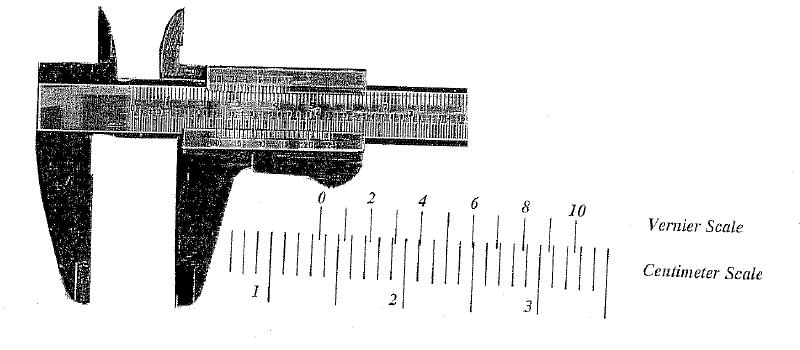
\includegraphics[width=6in]{vernier.JPG}
\vspace{-.25cm}
\caption{The Vernier Caliper:  The location of the zero on the vernier scale tells you where to read the centimeter scale (1.3 cm).  The vernier-scale line that lines up tells you the next digit (5).  This picture measures $1.35\pm 0.01 \unit{cm}$.}\label{f:vernier}
\end{center}
\begin{center}
\hspace{-2cm}
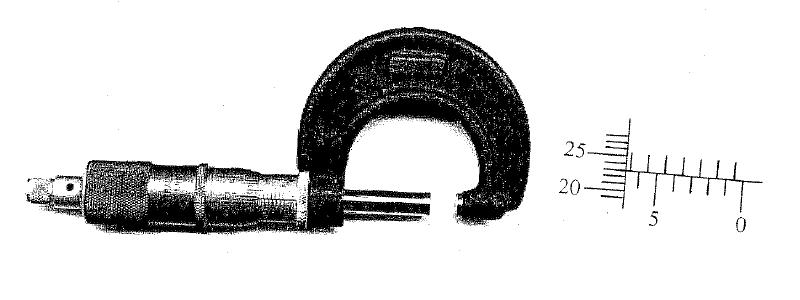
\includegraphics[width=6in]{micrometer.JPG}
\end{center}
\vspace{-.5cm}
\caption{The Micrometer Caliper:  Notice on the coarse scale, that the lower lines read (1, 2, 3, <ellipsis /> 6 in this picture) and the higher lines read the half-marks (0.5, 1.5, 2.5, <ellipsis /> 6.5 in this picture).  The location of the turning dial tells you where to read the coarse scale (6.5 mm).  The center line of the coarse scale tells you where to read the fine scale.  This is 23.0 (in units of $\times 10^{-2}$ mm), but not 23.5 and not 22.5 so the precision is 0.5 (in these units).  This measurement in mm reads $6.5 \unit{mm} + 0.230\unit{mm} = 6.730 \pm 0.005 \unit{mm}$. }\label{f:micrometer}
\vspace{-.5cm}
\end{figure}
%

%-------------------------------------------------------------------------------------
\onecolumn

\section{Standard Deviation}
\revised{Aug. 28, 2009}
\revision{Aug. 28, 2009}{Added Jack's picture back in}
\revision{Jan. 7, 1997}{Jack}

\subsection{Introduction}

Suppose you are standing in front of a dart-board.  You have a large number of darts and you throw the darts one at a time, trying to hit a 1 cm thick vertical line drawn on the dart-board.  Since you have a very good aim, let us say that 45\% of the darts hit the line.   This then means that you miss the line 55\% of the time; with a significant number of these misses being between .5 to 1.5 cm either to the left or to the right from the center of the line, and with a smaller number of misses being between 1.5 to 2.5 cm from the center line.

Is there some mathematical way of characterizing how good you are at this game?  What, for example, is the probability of missing the line by 1 cm?  The statistical analysis of random fluctuations in data can help answer these questions.   The word ``statistical'' implies that a relatively large set of similar measurements of a given physical quantity is available.  The random fluctuations in the data can be measured with the use of a mathematical term called the ``standard deviation.''

Suppose you collect data on a large number of throws, separating the data into categories (bins): The number of darts on the line, the number within .5 to 1.5 cm from the center, the number within 1.5 to 2.5 cm, etc.  A plot of this data with the dart positions on the x-axis and the number of darts hit within each bin plotted on the y-axis is called a histogram (see Figure~\ref{f:histogram}).  The envelope of this graphical data set is bell shaped, and is called a Gaussian or a Normal distribution curve.
%
\begin{figure}[bhtp]
\begin{center}
%\begin{picture}(400,200)
%\put(0,0){\line(0,1){200}}
%\put(0,0){\line(1,0){400}}
%\put(200,195){\vector(0,-1){25} $\mu$}
%\put(200,100){\vector(1,0){75}}
%\put(200,100){\vector(-1,0){75}}
%\put(200,105){$\sigma$}
%\end{picture}
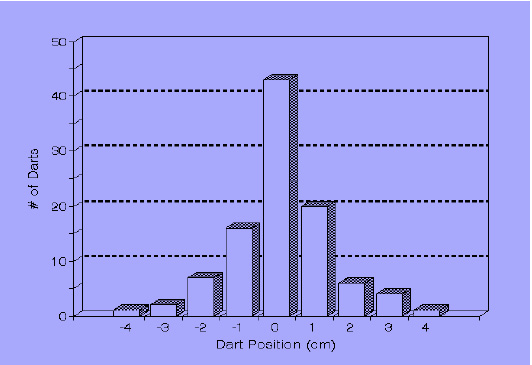
\includegraphics[height=2.5in]{darthistogram.jpg}
\caption{Histogram for the number of darts binned by distance from the centerline.}\label{f:histogram}
\end{center}
\end{figure}


The ``standard deviation'' is a measure of the spread or width of the histogram data.  A small standard deviation  means that there is a small spread in the data about the central mean value and implies that the data cluster closely about one value.   That is, there is a high degree of precision in the measurements.


The area beneath the curve, or below a part of the curve represents the probability of occurrence.  For example, the area beneath the curve between plus and minus one standard deviation from the mean represents a 68\% probability of your next throw falling within this range.  The area beneath the curve between plus and minus two standard deviations from the mean represents a 95\% probability of your next throw falling within this range.

In this experiment, you will study the use of the ``standard deviation'' in the statistical analysis and probability involved with flipping pennies.
\subsection{Experimental Purpose}

The goal of the experiment is to determine how the mean, standard deviation, and standard deviation of the mean depend on the amount of data (number of samples) taken.  You should also consider how well the data fit to a normal distribution.

\subsection{Student Outcome}

In this experiment, you should learn
\begin{enumerate}
\item the formulas for and the roles of the mean, the standard deviation, and the standard deviation of the mean in the statistical analysis of data containing random errors,
\item how to create histograms and scatter plots,
\item how to include trendlines on scatter plots, and
\item why more data is always better.
\end{enumerate}

\subsection{Pre-Lab Work}
\begin{lablist}
\item Define the following, both in a sentence and with a mathematical formula:  mean, standard deviation (sometimes called the standard deviation of a single observation), and standard deviation of the mean.  Be sure to describe the difference between these two terms.
\item Define the following:  histogram, probability, \& probability distribution (Normal distribution).
\item What does the total area under the Normal distribution curve represent?
\item How should the axes of the histogram of the data you will take for this lab be labeled?  Give a very specific scale for the x-axis.  (Hint: Read the procedure below.)
\item Make a sketch of an inverse function, like $y=1/x$.
\end{lablist}

%\twocolumn[\vspace{-.5cm}
\subsection{Experimental Procedure}

Each individual will receive 20 pennies and will then simultaneously toss all of the pennies.  Count the number of heads, and repeat 25 times.   Each individual will then have collected 25 pieces of data.
%\\]

\subsection{Analysis}

\begin{lablist}
\item Calculate the mean, the standard deviation  and the standard deviation of the mean for your first ten tosses and for all 25 tosses.  Show your calculations.
\item Make a histogram plot (by hand in your note book) for your 25 tosses.   On this histogram superimpose a sketch of your best guess of the corresponding Normal distribution curve.
\item How well does your data fit a normal distribution curve?  Explain the reasons for any large discrepancies.
\item Obtain histograms and calculations of the mean, the standard deviation and the standard deviation of the mean for the following data sets:  i) your lab group,  ii) about 1/2 of the class, and iii) the entire class.   These histograms can be obtained with the use of a computer program, provided by the instructor.
\item Draw graphs of:  the mean, the standard deviation, the standard deviation of the mean, versus the number of data entries.   Use the standard deviation of the mean  as the error bars for both the mean and the standard deviation,  draw these error bars on these two graphs.
\item Describe how the values of the mean, the standard deviation, and the standard deviation of the mean, change as the number of data items in the set increases.  What does this infer about the accuracy and about the precision of the data as more and more observations are made?
\item Show that the standard deviation of the mean varies inversely as the square root of the number of data items in the sample.   How well does the data in this lab agree with this prediction?   (Make a graph of the standard deviation of the mean versus the square root of the number of data items in the sample.)
\end{lablist}

\subsection{Questions}
\begin{enumerate}
\item What is the probability of flipping the 20 pennies and getting 5 heads, or 8 heads, or 10 heads, or 15 heads?   Answer this question by analyzing your data, the entire class' data and the normal distribution curve fit to your data.  Explain any differences between these sets.
\item What percentage of your individual readings fall within plus or minus one standard deviation,  two standard deviations?   Compare your answer to the theoretical answer from a normal distribution curve.  What are the percentages for the class data?
\item Does the height of the histograms change as a function of the number of trials?  If so, how?
\item How does the width at 1/2 the maximum height for the histograms change as a function of the number of trials?  Label this width on your histograms.  Is this width a reasonable estimate of the standard deviation?
\item Does the standard deviation of a single observation and/or does the standard deviation of the mean change significantly as the number of tosses increase?  What does this infer about the accuracy and about the precision of the data as more and more observations are made?
\end{enumerate}

\subsection*{Resource Materials}

Meyer, \underline{Data Analysis for Scientists and Engineers} John Wiley, (1975) p.19-48, 223-253


%-------------------------------------------------------------------------------------
\onecolumn

<chapter><title>Constant Acceleration</title>
<!-- Revisions
\revised{Sept. 14, 2015}
\revision{Sept. 14, 2015}{Commented out Graphs and Tracks.  Updated Pasco Reference from DataStudio to Capstone}
\revision{Sept. 16, 2008}{Created?}
-->

    <objectives><title>Experimental Purpose</title>
    <introduction><p>Using position versus time and velocity versus time graphs, verify that the equations of constant acceleration accurately describes the behavior of objects under constant acceleration and that it is possible to distinguish acceleration due to gravity from acceleration due to friction.</p>
    </introduction>
    </objectives>

    <section><title>Student Outcomes</title>
    <p>In this exercise, the student should develop an understanding of the relationships between the position and the instantaneous velocity of an object, as well as how each of these can vary as functions of time.   We will only consider the special case where the object experiences constant acceleration.</p>

    </section>

    <section><title>Materials</title>
    <p>An aluminum track, a low-friction cart, computer interface with PASCO Capstone<m>^{\rm tm}</m> software, a sonic motion sensor, a small steel ball.</p>
    </section>

    <section><title>Procedure (to be paired with Section~\ref{ss:AccAnalysis})</title>

    <subsection><title>Cart and Flat Track</title>\label{sss:FlatTrack}
    <p>Log into the computer (so you can save your data to your network drive) and then open Pasco Capstone.
    (Section~\ref{s:Capstone} will provide some instructions for setting up the software and connecting the equipment.)
Connect the motion sensor to the computer interface.
Set the data rate of the motion sensor at <m>50 \unit{Hz}</m>.
Place a steel ball on the track and adjust the leveling screw at one end of the track to see if the ball rolls one way or the other.  This will roughly level your track.
Place the sensor about 20 cm from the end of the track, because this is the minimum distance detected by the sensor.  (You might need to use the <q>sail</q> for the sensor to see the cart.)</p>

    <p>Place the cart on the track.  Capstone, via the sonic ranger, can measure the position and velocity of the cart as a function of time.  (This is explained in Section~\ref{s:Capstone}.)
<ol>
<li><p> Assume the track is frictionless and predict how the cart will move if the track is not perfectly level; include a comment about how the velocity versus time graph will look when it goes uphill versus when it goes downhill.  Should these be the same?
</p></li> <li><p> What do you expect the graph to look like if the track <em>is</em> perfectly level?  Will it be the same going left versus going right?
</p></li> <li><p> Now, assuming it is perfectly level, what will friction do to the motion?  How do you expect this to affect the graphs?
</p></li> </ol>
\setcounter{dave}{\theenumi}
</p>

    <p>We will take four sets of data: a slow, constant velocity towards the ranger; a slow, constant velocity away from the ranger; a faster, constant velocity towards the ranger; and a faster, constant velocity away from the ranger.  The two slow speeds should be about the same and the two faster speeds should be about the same.  For each case, start the sonic ranger and then bump the cart firmly, but not violently(!).</p>

    <p>On Capstone, you should have four curves of velocity versus time.  Fit each with a trendline and display the equation of the trendline on the screen.  Interpret the coefficients (slope and intercept) by noting their units, values, and uncertainties.  You should also print out (in landscape mode) the position versus time graph, the velocity versus time graph, and the acceleration versus time graph.  (You should notice that the acceleration versus time graph is <em>very</em> noisy.)</p>

    </subsection>
    <subsection><title>Cart and Sloped Track</title>\label{sss:SlopedTrack}
    <p>Place a small block under one end of the track, so that the track is now tilted at a small angle with the sensor at the top of the incline.  Measure the angle using a protractor or calculate it by measuring the two legs of the triangle and using the inverse sine.  (Be careful about measuring the height.)</p>

    <p.>We will consider <em>three cases</em> for the sloped track: <em>First</em>, allow the cart to roll (without an initial push) down the ramp.  <em>Second</em>, gently push the cart down the ramp.  DON'T let it fly off or crash into anything.
<ol>
\setcounter{enumi}{\thedave}
<li><p> Should these two cases have the same acceleration while rolling down the ramp?  How will that affect the shape of the velocity versus time graphs?
</p></li> <li><p> Should these have the same initial velocity?  How will that affect the graphs?
</p></li> </ol>
\setcounter{dave}{\theenumi}
In the <em>third</em> case, start the cart at the bottom of the incline and roll it up the ramp, allowing it to roll back down on its own.  Push it hard enough to get mostly up the ramp, but not so hard that it hits the sonic ranger.
<ol>
\setcounter{enumi}{\thedave}
<li><p> Should this case have the same acceleration while it goes up the ramp as while it goes down the ramp? How can we see that on the velocity versus time graphs?
</p></li> <li><p> Should this case have the same acceleration (either while it goes up the ramp or while it goes down the ramp) as the previous two cases of rolling down the ramp?
</p></li> </ol>
\setcounter{dave}{\theenumi}
</p>

    <p>In Capstone, you should be able to display all three graphs (position v time, velocity v time, and acceleration v time).  You should also be able to display all three cases of data on each of these graphs.  On the velocity versus time graph, fit each of the three graphs with a linear trendline.  The next section will ask you to analyze how well the data match up to these lines.  (It might be interesting to also fit the position vs time curves to parabolas.  Be sure to print out copies of your three graphs.</p>

    <p>Your lab should note the following results and explain their meaning:  slope and y-intercept, the uncertainties (precision) in both the slope and intercept, and the <m>r</m> value (correlation coefficient). </p>

    </subsection>
    </section>

    <section><title>Further Analysis and Discussion</title>\label{ss:AccAnalysis}

    <subsection><title>Cart and Flat Track</title>

    <p>Based on the results of Sec.~\ref{sss:FlatTrack}, write a short analysis of the relationship between these two graphs (x and v versus time).   From the velocity versus time graph (specifically from the trendline) determine the value of the acceleration of the cart down the track; be sure to include the uncertainty of the acceleration and the units.
<ol>
<li><p> Do you see any evidence that the track was not perfectly level?
</p></li> <li><p> Do you see any evidence that there is any friction as the cart moves along the track?
</p></li> <li><p> What does the intercept of the velocity versus time graph tell you?
</p></li> <li><p> If the slopes are different, then discuss any pattern that you see.  If the slopes are (essentially) the same, then find an average and a standard deviation of the four values.
</p></li> <li><p> Does it matter how fast the cart travels?
</p></li> </ol>
\setcounter{dave}{\theenumi}
    Discuss any evidence observed in your data when answering these questions.  Also consider the magnitude of the uncertainties when writing your conclusions.</p>

    </subsection>
    <subsection><title>Cart and Sloped Track</title>

    <p>Based on the results of Sec.~\ref{sss:SlopedTrack}, write an analysis of the relationship between the two graphs
(x and v versus time).  From the velocity versus time graph determine the value of the acceleration of the cart down the track.
<ol>
\setcounter{enumi}{\thedave}
<li><p> For the two downhill cases, use your uncertainty analysis to determine if the acceleration of the cart changed when it was given a small push.
%</p></li> <li><p> For the case that you copied into Excel, compare the results for the acceleration (with uncertainties) between <q>Data Studio</q> and Excel.  Comment on any differences.
</p></li> <li><p> Is there an accuracy<fn>If the track were frictionless, then the acceleration should be <m>a=(9.81\unitfrac{m}{s^2})(\sin\theta)</m>, where <m>\theta</m> is the angle that the incline makes.</fn> that can be computed for this part of the experiment?
</p></li> </ol>
\setcounter{dave}{\theenumi}
%
Inspect the line/curve that is defined by the data on the Distance traveled vs. time graph.
<ol>
\setcounter{enumi}{\thedave}
<li><p> What is its shape?  Is the shape of the graph what you would expect for constant acceleration (straight line, parabola, etc.)?  Explain your reasoning.
</p></li> <li><p> Consider the trendline that you added.  Does/should the trendline line go through the origin?  What is the value of y-intercept of the X vs T graph?  What physical quantity does the intercept represent?  Explain why it has that value.  Hint: (Think about where the sensor was located.)
</p></li> <li><p> What does the slope (whether it's constant or not) of the line on this graph signify?
</p></li> </ol>
\setcounter{dave}{\theenumi}
Now consider the Instantaneous Velocity  vs. Time graph.
<ol>
\setcounter{enumi}{\thedave}
<li><p> Does the curve/line on this graph have the shape you would expect for an object undergoing constant acceleration? Explain.
</p></li> <li><p> What was the value of the y intercept on this graph (include units and uncertainty!)?  Explain its significance.  To what does it refer?  Think carefully about what you plotted on the X-axis!
</p></li> </ol>
    </p>

    </subsection>
    </section>
</chapter>

%-------------------------------------------------------------------------------------
\onecolumn

<chapter><title>Newton's <m>2^{\rm nd}</m> Law on a Linear Track with the Sonic Ranger</title>\label{s:Newton}
<!-- Revisions
\revised{Sept. 14, 2015}
\revision{Sept. 14, 2015}{Updated Pasco Reference from DataStudio to Capstone}
\revision{Sept.~23, 2008}{}
-->

<introduction><title></title>Introduction to Forces}

Forces are related to the natural motion of bodies, where one object can affect the motion of another object.  That is, forces are interactions between objects affecting their motion.  Although the famous Greek philosopher Aristotle claimed that a force was necessary to <em>maintain</em> any motion, careful analysis by Italian physicist Galileo Galilei in the mid-<m>17^{\rm th}</m> century and by Sir Isaac Newton, a British mathematician and physicist (1642-1727), eventually distinguished the effects of friction and allowed Newton to create a mathematically consistent theory of motion.  These concepts were published in Newton's book <q>Mathematical Principles of Natural Philosophy</q> in 1687, for which (among other accomplishments) Newton is regarded as one of the greatest scientists of all time.

All forces can be placed in one of two main categories.  First, there are natural (or fundamental) forces like the gravitational force, the electromagnetic force, or the nuclear forces.  The gravitational force is a force on a body by another body (like the Earth), this force is an interaction between their two masses.  The electromagnetic force is an interaction between the charges of two bodies.  These forces may act on an object without any direct physical contact between the two bodies.  This type of force is sometimes called an <q>action at a distance</q> force.  All other forces are in a second category called <q>contact forces.</q>

<subsection><title></title>Newton's First law}

<quote>
If there are no forces acting, then objects will remain at rest or, if not at rest, will maintain their velocity.
</quote>
If this is true, then we can study the forces acting on a body based on the motion of the body, specifically through the change in the velocity of an object.

</subsection>
<subsection><title></title>Newton's Second Law}

Not only is a force necessary to change the motion (to cause an acceleration), the amount of acceleration that a force causes is predictable and is inversely proportional to the mass.  The same sized force causes a small mass to accelerate a lot and a large mass to accelerate a little.  this is expressed by the equation:
<me> \vec F_{\rm net} = m \vec a. </me>
The net force, <m>\vec F_{\rm net}</m>, is the vector sum of all forces acting on an object.  If we have an extended object (such as a weight hanging off of a table, but connected to a cart that is on the table), then we need only consider forces that are <q>external</q> to the system:  So long as both objects accelerate at the same rate, we do not need to consider the <q>internal</q> tension that the string exerts between the connected bodies.

</subsection>
<subsection><title></title>Newton's Third Law}

Inherent in the description of a force is that it is an interaction between objects: there must always be two objects that interact.  These objects exert equal and opposite forces on each other.  That is,
<quote>
If there is a force exerted on object 1 by object 2, then there is necessarily and simultaneously a force exerted on object 2 by object 1 that is equal (in magnitude) and opposite (in direction) to the original force.
</quote>
Remember that these two forces are on different objects and that the two bodies in direct contact exert forces on each other.  Remember then that if there is contact between the object (any part of the system) and anything else then there is an outside force on the object (system) and that if there is no contact (the two bodies break contact) then there is no force.


</subsection>
</introduction>
    <objectives><title>Experimental Objective</title>

    <introduction><p>In this experiment, we will assume that the first law is true and focus on the second law.
    By measuring (a) the velocity versus time for a cart being pulled down a track and (b) the applied force that is pulling it, we can plot the acceleration versus the force and verify the validity of Newton's second law of motion: <m>\vec F_{\rm net} = m \vec a</m>.</p>
    </introduction>
    </objectives>

</section><section><title></title>The Experimental Setup}

<ul>
<li><p> A low-friction linear cart and track will be used, this reduces the friction between the cart and the track.
</p></li> <li><p> A string will be connected to the cart and a known mass will be hanging from the end of the string (and over a pulley).   The hanging mass will exert a constant horizontal force on the cart as the mass falls all the way to the floor.  This gives a constant acceleration to the cart.
</p></li> <li><p> The sonic motion sensor will be used to measure the position of the cart as a function of time.
</p></li> <li><p> The carts and tracks need to be handled with care.  Scratches can add friction to the system.
</p></li> </ul>

</section><section><title></title>Pre-Lab Work}

<ul>
<li><p> Draw a free-body force diagram for the cart and for the hanging mass.
</p></li> <li><p> Derive an equation for the acceleration of the system, in terms of, the mass of the cart and the hanging body.
</p></li> </ul>

</section><section><title></title>Procedure}

<ul>
<li><p> If the cart is given an initial push (without the hanging mass and string attached) then the cart should travel with a constant velocity down the horizontal track, if there are no other forces acting on the cart.  Carry out  a couple of constant velocity runs on the track, to check for the effects of friction and to see how level the track is. The track may need a level adjustment.  Do runs in both directions.  Maybe the track can be tilted so that the friction is countered by the tilt of the track.
</p></li> <li><p> Connect a string to the cart and run it through the hole at the end of the track, then over a pulley.  Make sure that the string is horizontal.  Measure the height of the string at both ends of the track, to see if the string is horizontal.
</p></li> <li><p> The hanging mass should be much less than the mass of the cart.  Use a small plastic cup to hold the hanging masses.   Measure the mass of  this cup.  The total mass of the system must be kept constant for all parts of the experiment.   The hanging mass and the mass of the cart should vary, but their total must be kept constant, by moving small mass amounts from the cart to the hanging cup.  Record the mass of the cart, the hanging cup mass, and the extra masses which are to be transferred from the cart to the cup.
</p></li> <li><p> Take data with Capstone and the motion sensor as the cart travels with constant acceleration down the track.   Determine the acceleration of the cart from a linear regression using the velocity vs time data (a linear fit line in Capstone).  Record the acceleration value and its uncertainty.
</p></li> <li><p> Collect  7 data runs, where about 5 grams is transferred each time from the cart to the hanging mass.   Determine the acceleration of the cart (and the uncertainty for the acceleration) for each of these 7 runs.
</p></li> </ul>

</section><section><title></title>Analysis}

<ul>
<li><p> Make a graph of the acceleration of the system (y-axis) versus the weight (<m>mg</m>) of the hanging body (x-axis),  should include 7 data points.    Do this in Excel.   Carry out a linear regression for this data set.   Quote the  slope and intercept values, their uncertainties, their p-values, and the <m>R^2</m> value.     Show a sample error bar (on the graph) for at least one of the points of this graph.
</p></li> <li><p> Derive (show it completely)  an equation for the acceleration of the system versus the weight of the hanging body.  Plot this theory equation on your graph (as a second series, a line but no points).
</p></li> <li><p> Compare your graph to the predicted theoretical equation, that is compare the values of the slopes and intercepts.  What is the physical significance of the slope and of the intercept from the graph?  That is, what physical quantity does the slope of this graph equal?
</p></li> <li><p> In many mechanics experiments, there may be deviations from the expected or theoretical results because of the effects of friction.  Frictional forces are sometimes difficult to take into consideration.  If there are deviations between your results and the predicted theory then try to distinguish whether they are caused by a tilt of the track, friction between the cart and the track or the friction between the string and the pulley.  What might be expected in the results from these different systematic effects?    That is, would the slope be expected to increase or decrease slightly because of the effects of friction?
</p></li> <li><p> When designing experiments, it is important to keep control parameters; in this case a parameter which is kept constant.   What parameter held this role in this experiment?
</p></li></ul>

%\vfill\hfill(<m>\hookrightarrow</m>)
%\onecolumn
</section><section><title></title>Questions}

<ol>
<li><p> Why is it important to keep the total mass of the system constant?   What would happen if the total mass of the system was not held constant?    If one simply added mass to the hanger without keeping the system's mass constant,  how would their data appear on the graph of the acceleration vs <m>mg</m>?
</p></li> <li><p> What would happen if the track was not level?   If the beginning end of the track is higher,  how would the acceleration of the system be affected?
</p></li> <li><p> If your group has a discrepancy between the results and the theory, could friction be used to explain your results?   Explain how.   In this case, how much of a tilt in the air track would be needed to explain the discrepancy?   Show this calculation.
</p></li> <li><p> What would happen to the cart's acceleration if the cart was given an initial push?
</p></li> <li><p> What are the two greatest sources of uncertainty in this experiment?   Are they random or systematic errors?   Be specific and quantify your answer.
</p></li> </ol>


</chapter>

%-------------------------------------------------------------------------------------
\onecolumn

<chapter><title>Dry Sliding Friction</title>
<!-- Revisions
\revised{Sept.~28, 2015}
\revision{Sept.~28, 2015}{}
\revision{Sept.~23, 2008}{}
-->

<introduction><title></title>Introduction}

Friction is a force which retards the relative motion of any body while sliding over another body.  The frictional force acting on a body is parallel to the surface that the object is sliding upon and it is directed opposite to the direction of motion.  The phenomenon of friction is rather complicated, especially at the microscopic level, because it is dependent on the nature of the materials of both contacting surfaces.  The frictional force depends on the roughness or the irregularities of both surfaces.  At the macroscopic level, the nature of this force can be described by a simple empirical law, first given by Leonardo da Vinci:
<quote>
The magnitude of the force of friction between unlubricated, dry surfaces sliding one over the other is proportional to the normal force pressing the surfaces together and is independent of the (macroscopic) area of contact and of the relative speed.
</quote>
At the microscopic level, the frictional force <m>(F_f)</m> does depend on the actual area of contact of the irregularities of the surfaces.  This actual area of contact then increases as the force pressing the two surfaces together increases, this force is called the load.  Using Newton's <m>2^{\rm nd}</m> Law in this perpendicular direction we can conclude that the magnitude of the load is equal to the Normal force <m>(F_N)</m> of the surface pushing on the object.  Therefore we may write that
%
<me>
F_f \propto F_N
\mbox{\ \ \ \ or \ \ \ \ }
F_f = \mu F_N
</me>
%
where the Greek letter <m>\mu</m> (<q>mew</q>) is a dimensionless constant of proportionality called the coefficient of friction.

When a body is pushed or pulled parallel to the surface of contact and no motion occurs, we can conclude that the force of the push or pull is equal to the frictional force, using Newton's <m>2^{\rm nd}</m> Law of motion.  As the applied force is increased, the frictional force remains equal to the applied force until motion results.  At this maximum value of the applied force, the frictional force is also a maximum and is given by
%
<me>
F_f = \mu_s F_N
</me>
%
where the subscript <m>s</m> stands for static (non-moving) friction.  This equation can only be used at this maximum static point also called the point of impending motion.  At the instant that the applied force becomes greater than the maximum fs, the body is set into motion and this motion is opposed by a frictional force called the kinetic (sliding) frictional force and is given by
%
<me>
F_f = \mu_k F_N
</me>
%
where the subscript <m>k</m> stands for the kinetic (moving) friction.  In general, <m>\mu_k < \mu_s</m>; that is, it takes more force to overcome the static friction than to over come the kinetic friction.  The coefficients of friction are generally less than one, but may be greater than one, and they depend on the nature of both surfaces.



	Consider a system comprised of a block on a horizontal surface being pulled horizontally by a string connected to a hanging weight.   Assume that the system is accelerating with a constant acceleration.  Then the <m>\mu_k</m> can be solved for by the following equation:
%
<me>
\mu_k  = \frac{ mg - (M+m) a }{ Mg},
</me>
where <m>M</m> is the mass of the block and <m>m</m> is the hanging mass.


    </introduction>
    <objectives><title>Experimental Objective</title>

    <introduction><p>In this experiment you will devise methods to investigate the nature of both the frictional force and the coefficient of friction, and to test the validity of da Vinci's empirical rule.</p>
    </introduction>
    </objectives>

<section><title></title>Pre-Lab Analysis}

<ul>
<li><p> Draw force diagrams for the following case:     a block on a horizontal surface pulled by a hanging mass and a string  (include the friction force).
</p></li> <li><p> Write out the corresponding Newton's <m>2^{\rm nd}</m> Law equations for forces both parallel and perpendicular to the contact surface.
</p></li> <li><p> Derive the relevant equations for each of the above two cases for which the coefficients of friction can be determined:
    <ul>
    <li><p> Case one is static, but at the point of motion.
    </p></li> <li><p> Case two is the kinetic case.
    </p></li> </ul>
</p></li> </ul>


</section><section><title></title>The Experiment}

For the block on the horizontal plane:	
<ol>
<li><p> Clean the block and the plane, so that they are free of dust and other contaminants.  \\
Make sure the track is level, as in previous labs.
</p></li> </ol>
\setcounter{dave}{\theenumi}

</subsection><subsection><title></title>Break Static Friction - pull until moves}\label{sss:staticfriction}
<ol>
\setcounter{enumi}{\thedave}
<li><p> Set up the Dynamics Track, cart, force transducer and friction block.  The force transducer attaches to the dynamics cart, the friction block rests on the track (felt side down).
</p></li> <li><p>\label{i:staticpull} Attach a string to the force transducer.  The force transducer needs to be zeroed before data collection starts.  Collect data, and slowly start pulling on the string (<em>be sure to pull the string horizontally</em>) and slowly increase the pull force until the cart is moving down the track. Using just the maximum force (at the point of impending motion) the coefficient of static friction can be calculated.
</p></li> <li><p>\label{i:statictest} Test the relationship between the force of friction and the normal force, by changing the load force (normal force) and measuring the force of friction at the point of motion impending. Carry this out for a total of five data points.  Graph the frictional force versus the normal force.  Calculate the coefficient of static friction from this graph.
</p></li> </ol>
\setcounter{dave}{\theenumi}

</subsection><subsection><title></title>Effect of Surface Area - distinguish pressure from force}\label{sss:friction-area}

Consider pushing a pencil into your arm. (Well, don't <em>actually</em> do it!)  If you use the erasure end, then you can feel the force, but it doesn't hurt.  If you use the sharpened tip with the <em>same</em> force then it will certainly hurt!  So, you have the idea that the same force spread over a different surface area <em>can</em> have a different effect; but it doesn't <em>always</em> have a different effect.  For this part of the lab, you will test the relationship between the coefficient of friction and the macroscopic area of contact between the block and the surface.
<ol>
\setcounter{enumi}{\thedave}
<li><p> Place the friction block on its side (felt side down) and repeat Steps~\ref{i:staticpull} and~\ref{i:statictest} for three (rather than five) of the previous load forces.
</p></li> <li><p> Add the plot of this <m>F_f</m> versus <m>F_N</m> as a new series to the graph of Part~\ref{sss:staticfriction}.
</p></li> </ol>
\setcounter{dave}{\theenumi}

</subsection><subsection><title></title>Friction while Accelerating}

<ol>
\setcounter{enumi}{\thedave}
<li><p> Apply a force (hanging mass, pulley, and string) large enough to accelerate the block. Use the Sonic Ranger to collect data.
</p></li> <li><p> Graph the velocity vs time.  Determine the acceleration of the block from the slope of the line.
</p></li> <li><p> Repeat this part four or five times with a different normal forces.  (You may use any hanging mass.)
</p></li> <li><p> Add the plot of this <m>F_f</m> versus <m>F_N</m> as a new series to the graph of Parts~\ref{sss:staticfriction} and~\ref{sss:friction-area}.
</p></li> <li><p> Calculate the coefficient of kinetic friction from the slope.
</p></li> </ol>



</section><section><title></title>Analysis}
<ul>
<li><p> The experimental precision should be estimated for all parts of this experiment and care should be taken for all of the measurements, but it is more important to investigate the relationships than it is to repeat the experiment many times or to try to achieve high precision in the data.
</p></li> <li><p> Explain why the normal force on the block by the surface rather than the weight of the object is related to the frictional force.
</p></li> <li><p> Interpret the slope and intercept of the graphs.
</p></li> <li><p> Compare the slopes from each of the three parts.  Decide which should be the same and which should be different.
</p></li> <li><p> Calculate the \% decrease of the static to kinetic coefficient of friction.
</p></li> <li><p> Comment on the validity of the empirical rules of friction.
</p></li> </ul>


</section><section><title></title>Questions}

For all questions, and when possible, use your experimental or theoretical results to demonstrate your answers to the questions.
<ol>
<li><p> Does the coefficient of friction depend on the area of contact?
</p></li> <li><p> Does the coefficient of friction depend on the mass of the object?
</p></li> <li><p> Does the coefficient of friction depend on the normal force of the object?
</p></li> <li><p> Does the frictional force depend on the normal force of the object?
</p></li> <li><p> Does the coefficient of kinetic friction depend on the speed of travel?
</p></li> <li><p> When the object was pulled by a string, how would the forces be affected if the cord was not horizontal?
</p></li> <li><p> What would happen to the coefficient of friction if the surfaces were lubricated with oil?
</p></li> </ol>


</chapter>

%-------------------------------------------------------------------------------------


\onecolumn
<chapter><title>Centripetal Force</title>
<!-- Revisions
\revised{Fall 2006}
-->
<introduction><title></title>Introduction}

We will be investigating the force which is necessary to maintain the circular
motion of an object.
The apparatus used will allow you to spin an F-shaped arm which has a mass
suspended from the
top arm.  This mass will be held in place by a spring which makes up the lower
arm.  The spring
will provide the centripetal force.  You will need to be familiar with the
ideas of circular motion,
centripetal versus centrifugal force, centripetal acceleration, and angular
velocity.  In addition to
these concepts, try to understand how we will measure the angular speed in lab.

The centripetal acceleration <m>a_c</m> is calculated from the following equation
written either <m>\displaystyle a_c=\frac{v^2}{r}</m> or <m>\displaystyle a_c =
\omega^2 r</m>
where <m>v</m> is the linear velocity of the particle, <m>\omega</m> is the
angular velocity, and <m>r</m> is the radius of the circle.  Note that angular
velocity is measured in radians per second.

From Newton's second law, <m>\vec F = m \vec a</m>.
Therefore, the force required to keep the particle of mass <m>m</m> moving in a
circle
with constant speed is
%
<me> F = ma_c = \frac{mv^2}{r} = m\omega^2r </me>
%
Recall that the centripetal force is not a force applied <em>in addition</em> to
other existing forces.
The centripetal force is <em>whatever combination</em> of existing force act to
maintain circular motion.

    </introduction>
    <objectives><title>Purpose</title>

    <p>It is our purpose to verify the above equation experimentally by measuring the applied force
and comparing it to the specific combination of variables expressed as either
<m>\frac{mv^2}{r}</m> or <m>m\omega^2r</m>.</p>
    </introduction>
    </objectives>

<section><title></title>Pre-Lab}

<ol>
<li><p> Why do we say that an object moving with <em>constant speed</em> in a
circular path is being accelerated?
</p></li> <li><p> In which direction is that acceleration?  How do you know?
</p></li> <li><p> Is this <m>a_c</m> <q>centripetal</q> or <q>centrifugal?</q>
</p></li> </ol>

</section><section><title></title>The Experiment}

The centripetal force is supplied by a spring.  Since we cannot directly
measure <q>the
force exerted by the spring while it is rotating</q> while it is rotating,
determine how
we can measure <q>the force exerted by the spring during the
rotation</q>
when the spring is not rotating.

<ul>
<li><p>\label{i:r} By means of the lab apparatus, a mass <m>m</m> can be made to rotate with a constant (and measurable) angular speed <m>\omega</m>.  With some practice, it is possible to adjust the speed so that the radius of the path remains constant.  The value of the radius, <m>r</m>, is marked on the apparatus and so can be measured easily.
</p></li> <li><p>\label{i:m} Measuring the mass should be an obvious task.
</p></li> <li><p>\label{i:w} Measuring the angular speed <m>\omega</m> is straightforward, but may not be obvious.  To do so, consider the following:
    <ul>
    <li><p> Angular speed <m>(\omega)</m> is measured in <m>^{\rm radians}\!\!/_{\!\rm second}</m>.
    </p></li> <li><p> <m>\omega</m> is related to the rotational speed which is measured in <m>^{\rm revolutions}\!\!/_{\!\rm second}</m>.
    </p></li> <li><p> There are <m>2\pi</m> radians in 1 revolution.
    </p></li> <li><p> We can count the number of revolutions.
    </p></li> <li><p> The <q>period of rotation,</q> <m>T</m>, is defined as the number of seconds per revolution.
    </p></li> <li><p> We measure the period not by timing a single revolution, but by measuring the time for multiple (20) revolutions divided by the number of revolutions. (This averages out any uncertainty due to reaction-time.)
    </p></li> </ul>
</p></li> <li><p>[] As the mass rotates, its period of rotation can be measured.  This allows you to calculate the angular speed using the hints above.
</p></li> <li><p> Repeat the entire procedure for a second value of r.
</p></li> </ul>

</section><section><title></title>Analysis}

From measurements of <m>m</m>, <m>\omega</m>, and <m>r</m>, calculate the theoretical centripetal force on
the mass (which experimentally is supplied by the spring).  The (unmeasurable) amount
of force exerted by the spring to hold the spinning mass at a particular radius is
equal to the (measurable) force required to stretch the spring to that radius.  Experimentally determine
the force necessary to stretch the spring to a specific radius and compare that with the amount
of centripetal force calculated above.
</chapter>

%-------------------------------------------------------------------------------------

\newpage

<chapter><title>Conservation of Energy on a Linear Track</title>
<!-- Revisions
\revised{October 24, 2015}
\revision{October 24, 2015}{made it a one week lab}
\revision{August 24, 2009}{}
-->

<introduction><title>Introduction</title>

Conservation laws play a very important role in our understanding of our physical world.  For example, the law of conservation of energy can be applied in all physical processes.  This is a fundamental and independent statement about the nature of the physical world.  It is not necessarily derivable from other laws like Newton's Laws of motion.  Though for simple point mass systems, the law of conservation of energy can be derived from Newton's Laws.  It can be shown that the net work done on a system is equal to the change in the kinetic energy <m>(W_{\rm net} = \Delta K)</m> of the system; this is called the work-energy theorem and it can be written in a variety of forms.  When a net positive work is done on a system, the kinetic energy of the system increases, and when a net negative work is done on the system (as from a friction force), the kinetic energy of the system decreases.

When the gravitational force acts on a system, the work it does on the system, <m>W_g</m>, is the gravitational force <m>(mg)</m> times the vertical displacement <m>(h=\Delta y)</m>: <m>W_g=mg\Delta y</m>.  For convenience, this is called the change in gravitational potential energy <m>(W_g = - \Delta P)</m>.  <em>If</em> the gravitational force is the only force acting on the system then <m>W_g = W_{\rm net}</m> and therefore, <m>-\Delta P = \Delta K</m> for the system.  When a force can be associated with a potential energy, it is called a <q>conservative force.</q>  Another kind of potential energy deals with an elastic potential energy, like in a spring.  The energy stored in a spring is given by the formula <m>P_s = \frac{1}{2} k \Delta x^2</m>.

<em>If</em>, on the other hand, a force dissipates energy, then it is called a <q>nonconservative force</q> and it will have no associated potential energy.  Frictional forces are an example of a nonconservative force and the work done by a frictional force is negative because (physically) the frictional force removes energy from the system and (mathematically) the frictional force and the displacement are in opposite directions.  This work done by friction is converted into heat or sound.  To distinguish the energy of heat or sound from the potential and kinetic energy, we define the total mechanical energy, <m>E=K+P</m> at any point.  Since frictional forces remove mechanical energy, we say <m>W_f = \Delta E = \Delta K + \Delta P</m>.

In general then, the law of conservation of energy states that energy can not be created or destroyed, but can only change from one form to another; or the total energy of the system at point A is equal to the total energy of the system at point B.

    </introduction>
    <objectives><title>Experimental Objective</title>

    <introduction><p>The purpose of this experiment will be to verify the validity of the law of conservation of mechanical energy, that <m>\Delta E = 0</m> as a cart runs along a track.</p>
    </introduction>
    </objectives>

</section><section><title></title>The Experiment}

We would like for you to verify the conservation of mechanical energy in two different situations; so, there are two parts to this experiment.
We will first consider a flat track with accelerated motion, as in the Newton's Law lab and the Friction lab.  We can then consider an inclined plane.  You will not be given an explicit procedure, but rather you will be given a series of questions with answers that will imply the procedure.  Part of the experiment is for you to figure out for yourself what the best course of action is.  Please answer the questions as they are asked.

%There is enough analysis for this lab that you will have two weeks to complete the lab.  During the first week, you will do the two parts of the experiment and begin to write up your report.  During the second week, you will do some analysis and re-run the experiment to determine the cause of differences from expectations.  A single lab report will be due after the second week of experimentation.

</subsection><subsection><title></title>Flat Track}\label{sss:1flat}

Set up the dynamics cart on a horizontal dynamics track.  Set up the motion sensor at one end of the track and a pulley at the other end so that the pulley partly extends past the edge of the table.  Hang the basket over the pulley so that it can accelerate the cart along the track -- you might need extra weight in the cart to keep it from accelerating too fast.  In order to use this motion to verify the validity of the conservation of mechanical energy, we need to measure some variables.  Answer Questions~\ref{q:1KE} and~\ref{q:1PE} to decide on the relevant variables.  Question~\ref{q1:2or1} should help you determine how to finish setting up the equipment.

Once you decide what variables to measure, run the experiment for one set of masses while measuring the appropriate variables.  Put the data into Excel and decide what plot(s) will allow you to verify the validity of the conservation of mechanical energy.  Question~\ref{q:1plots} may help with this.  Decide if you need a trendline.  Relate the information in Question~\ref{q:1EKP} to the statement you are trying to verify.

%Save your data so that you can do further analysis next week.

</subsection><subsection><title></title>Sloped Track}\label{sss:1sloped}

Remove the pulley from the track.  Your cart will have either a spring-loaded <q>battering ram</q> on the front or a pair of magnets.  If you have the battering ram, then you will want the end of the track with the rubber nub at the bottom of the incline.  If you have the magnets, then you need to replace the pulley with a <q>C</q> shaped <q>catch-bar.</q>  <em>Ask for help from the instructor!</em>  The catch-bar has magnets in it that will repel the magnets in the cart.  In this case, the cart must not be going so fast as to come into physical contact with the magnets on the catch-bar.

Raise one end of the dynamics track.  Question~\ref{q:1slope} should help decide how tilted.  Measure the tilt angle of the track with two methods: use a protractor, and measure the vertical rise and track length and calculate the tilt angle using the inverse-sine function.  Answer Question~\ref{q:1anglemeasurement}.  As you continue to set up the track for measurements, consider answering Questions~\ref{q:1KE}, \ref{q:1PE}, and~\ref{q1:2or1} again for this situation to help you decide on the appropriate accessories (sensors); but note Question~\ref{q:1rampangle} as you think about the answers to the previous questions.

Once you decide on the variables to be measured, but before you make the measurements, you will need to calibrate your position measurements.  We would like zero to correspond to being at the bottom of the ramp, so place the cart stationary at the bottom and use the motion sensor to measure this position.  In order to verify the validity of the conservation of mechanical energy, release the cart from rest near the top of the ramp and let it roll down the incline, bouncing three times before you stop the measurement.  Do this for one value of mass.
%Answer Question~\ref{q1:mass}.

Transfer these data to Excel again and decide on the best graph to verify the objective.  Again, Question~\ref{q:1plots} may help with this; however, you will also need to consider Question~\ref{q:1bounce}.  Decide if you need a trendline and where it would be fit.  Relate the information in Question~\ref{q:1EKP} to the statement you are trying to verify.

%\newpage
</section><section><title></title>Additional Analysis}% -- Considerations during the second week}

%For the second week, you should already have your graphs from the experiment and you should have written a significant portion of the theory and the analysis.
We are now going to take a closer look at the irregularities of the data and investigate some variations to try to explain what those data say.

<ul>
%</p></li> <li><p> One of the factors you were asked to consider last week was Question~\ref{q1:mass}.  In order to verify this, re-run Part~\ref{sss:1flat} with a noticeably different massed cart.  Re-create the graph and use this only to note the effect of a different mass.  Answer Question~\ref{q1:mass2}.

<li><p> Before drawing conclusions about the validity of the conservation of mechanical energy, consider Question~\ref{q:1missing}.

%</p></li> <li><p> As you evaluate Part~\ref{sss:1sloped}, you might be asked to re-run the experiment with a force transducer placed at the bottom of the track.  (This should imply where the motion sensor will go.) Make sure that the cart will bounce from the force sensor. Make sure that the force sensor is zeroed before the start.  There might be some information here based on work as a force-through-a-distance versus work as a change-in-energy.

</p></li> <li><p> One explanation of a loss of energy (non-conservation) is friction.  List all of the places where two pieces of material rub against each other.  Since <m>F_f = \mu F_N</m>, do any of these locations have a normal force that can be varied?
    %(Recall Questions~\ref{q1:mass} and~\ref{q1:mass2}.)
    (Recall Question~\ref{q1:mass2}.)
    As an independent measure of the amount of friction, we can also consider the actual acceleration versus the expected acceleration.  Question~\ref{q:1accel} will help you determine the expected acceleration and the variable necessary to find it.  Question~\ref{q:1fracc} will help decide on the relationship between the friction and the acceleration.

</p></li> <li><p> A second explanation for the loss of energy is that some component is gaining rotational kinetic energy.  The formula for this is <m>K_R = \frac{1}{2} I \omega^2</m>, where <m>I</m> is the moment of inertia<fn>In this case, the moment of inertia is probably a little less than <m>\frac{1}{2} m r^2</m>, where <m>m</m> is the mass of the rotating object and <m>r</m> is the radius of the rotating object.  This is not a convenient way to calculate <m>I</m> at this time.</fn>, and <m>\omega</m> is the angular speed <m>\omega = v/r</m>.  Assuming that any discrepancy that you found in the conservation of energy is due to the rotational kinetic energy of the pulley, how much energy would the pulley need to have at the end of the run (while spinning full speed)?  Based on the final velocity of the cart, what is the angular speed of the pulley?  Based on these numbers, <m>K_R</m> and <m>\omega</m>, what is the moment of inertia for the pulley?   Can you tell if this is a reasonable estimate?
</p></li> </ul>


%\newpage
</section><section><title></title>Questions}

    <ol>
    <li><p>\label{q:1KE} In order to verify <m>\Delta E=0</m>, we will need to calculate <m>E</m> as <m>E=K+P</m>. Therefore, we need to know the kinetic energy, <m>K=\frac{1}{2} m v^2</m>, the energy of <em>some mass</em>, <m>m</m>, moving at a speed <m>v</m>.  Which mass do you need to measure?  How can you measure the velocity?
    </p></li> <li><p>\label{q:1PE} In order to verify <m>\Delta E=0</m>, we will need to calculate <m>E</m> as <m>E=K+P</m>. Therefore, we need to know the potential energy, <m>P=m g y</m>, the energy of <em>some mass</em>, <m>m</m>, located some height, <m>y</m>, above the ground.  Which mass do you need to measure?  How can you measure the position?
    </p></li> <li><p>\label{q1:2or1} In order to measure the position of the falling mass and the velocity of the system, do you need two motion sensors?  Can you manage with one?  Considering that it is a fairly expensive piece of equipment, where should you NOT put the sonic ranger?  Where could you put it?  Depending on where you put the ranger, decide if you need to <q>translate</q> the position or velocity data in order to find the specific values that you actually need.
    </p></li> <li><p>\label{q:1plots} To verify <m>\Delta E=0</m>, we will need to graph <m>E</m>, the total mechanical energy, as a function of time.  What do you expect this graph to look like, if the law is valid?  If not?
        <ol>
        <li><p> Does the kinetic energy change during this motion?  Is <m>\Delta K=0</m>?  Considering the initial and final values of the kinetic energy, <m>K_i</m> and <m>K_f</m>, what would a graph of <m>K</m> versus time look like?
        </p></li> <li><p> Does the potential energy change during this motion?  Is <m>\Delta P=0</m>?  Considering the initial and final values of the potential energy, <m>P_i</m> and <m>P_f</m>, what would a graph of <m>P</m> versus time look like?
        </p></li> <li><p> Assuming that the mechanical energy is conserved, what would a graph look like if it included <m>E</m>, <m>K</m>, and <m>P</m>?  What if the mechanical energy is not conserved?  How would <m>K</m> and <m>P</m> be affected in these two cases?
        </p></li> <li><p>\label{q:1bounce} (Part~\ref{sss:1sloped} only) When the cart is at the bottom of the track during the motion, the values of position become negative (less than zero!).  Why?  Is there some other place where the energy might go?  %If you are using the force transducer, then it has a spring and a spring potential energy, <m>\Delta P_{\rm spring}</m>.  This can (and should!) also be included in the total mechanical energy.  You can calculate the elastic potential energy stored in the spring of the force transducer with <m>P = \frac{1}{2} k \Delta x^2</m>, which, since we do not know <m>k</m>, can be written <m>P = \frac{1}{2} F \Delta x</m>, where F is the force in Newtons (measurable with the force transducer) and <m>\Delta x</m> is the distance from the spring's equilibrium position, not the height (derivable from the position data).  Be sure to match up the force values and the <m>x</m> values at those same times.
        </p></li> </ol>
    </p></li> <li><p>\label{q:1EKP} Please note the overall change in potential energy, <m>\Delta P</m>, and the overall change in the kinetic energy, <m>\Delta K</m>.  Should either of these be related to the overall change in energy <m>\Delta E</m> and, if so, how?
    </p></li> <li><p>\label{q:1slope}  We want the cart to accelerate down the track (not too slow), but not to fly off at the bottom (not too fast).  How fast is <em>too fast</em>?  Don't use that slope!  How fast is <em>too slow</em>?  Use a slope somewhere in between.
    </p></li> <li><p>\label{q:1anglemeasurement}  After you measure the angle of incline in these two ways, consider the uncertainty in the measurements.  Which of these measurement is more precise?
    </p></li> <li><p>\label{q:1rampangle}  The motion sensor will measure the motion of the cart <em>along</em> the ramp, but the potential energy needs the <em>vertical</em> position of the cart.  Which trig function relates the distance along the ramp to the corresponding vertical distance?
    %</p></li> <li><p>\label{q1:mass}  Does the mass of the cart matter?  If you run it again at a different value of mass, would you expect the overall conclusion to be different?  Would you expect the specific values to be different?
    </p></li> <li><p>\label{q1:mass2} If the mechanical energy is conserved, then
        <me> \frac{1}{2} m v_i^2 + m g y_i = \frac{1}{2} m v_f^2 + m g y_f </me>
        What do you notice about the mass?  Is your graph different if the mass of the cart changes?  Does this support or conflict with the idea that the total mechanical energy is conserved?  On the other hand, if the mechanical energy is not conserved, then
        <me> W_{\rm nc} = \frac{1}{2} m v_f^2 + m g y_f - \frac{1}{2} m v_i^2 - m g y_i</me>
        What do you notice about the mass now?  Does your graph support or conflict with the idea that the total mechanical energy is conserved?
    </p></li> <li><p>\label{q:1missing} We need to look for the energy lost in each graph.
        <ol>
        <li><p> When you look at the graph from Part~\ref{sss:1flat} for <m>E</m>, is the energy conserved or is there energy lost?   If lost, calculate the energy lost or gained from the graph. (It might help to have a trendline.)  If energy is lost, come up with at least two explanations for where this energy goes.
        </p></li> <li><p> When you look at the graph from Part~\ref{sss:1sloped} for <m>E</m>, there are jumps in the energy.  Why?
            <ol>
            <li><p> What is happening between the jumps?  Does Part~\ref{sss:1flat} help to explain these sections of the graph?  Compared to the jumps, can we assume that the mechanical energy is conserved between the jumps?
            </p></li> <li><p> What is happening at the time of those <q>jumps?</q>  From the trend of the graph, calculate the amount of energy lost during each sudden change, call it the energy discrepancy, and the percent of this discrepancy relative to the total energy before the corresponding collision.   Discuss where this <q>missing</q> energy goes.  Is the ratio of <q>energy discrepancy</q> to total prior energy the same for each jump?
            </p></li> </ol>
        </p></li> <li><p> Comment in general, on the law of Conservation of Mechanical Energy.  Can you predict any effects that might invalidate the conservation of mechanical energy?  Can these effects be minimized?  Is it possible to run the experiment again minimizing this effect?
        </p></li> </ol>
    </p></li> <li><p>\label{q:1accel} Given an ramp inclined at some angle <m>\theta</m>, what is the component of the gravitational force aimed down the ramp?  Assuming that there is no friction, what is the net force?  Since <m>F_{\rm net} = m a</m>, the acceleration should be <ellipsis /> ?<fn><m>a=g \sin\theta</m>.</fn>  From your expression, what do you need to measure in order to find the expected value of <m>a</m>?  (Recall Question~\ref{q:1anglemeasurement}.)
    </p></li> <li><p>\label{q:1fracc} If there is friction, then how do you expect the actual acceleration to compare to the expected acceleration?  If there is no friction?  So, how would you interpret finding an acceleration that is exactly equal to the expected value?  less than the expected value?  Larger than the expected value?
    </p></li> </ol>
</chapter>

%-------------------------------------------------------------------------------------

    \onecolumn

<chapter><title>Peer Review</title>
<!-- Revisions
\revised{Sep 1, 2008}
-->

<introduction>
<p>The most important part of doing science is the peer-review process.  After one completes a research project, the report is submitted for publication.  The publisher has a number of reviewer (usually made up of respected authors) and the submission is sent to two (sometimes three) reviewers who advise the publisher on the merits of the work.  Once you make a submission, it might be two months before the reviewers finish reviewing the work.  Generally the publisher will return the reviewers' comments to the author.  If all reviewers agree that the paper is viable, then the publisher accepts it.  If they agree not to accept a paper, then it is rejected.  If the reviewers are split, then the decision is at the discretion of the publisher.  In most cases, the reviewer makes suggestions for how to improve the paper or where to clarify the discussion.  In some cases, the author must either significantly revise the entire project or make an argument why the reviewer is either mistaken or is merely pointing out the specific point-of-contention that the author was intending to spark in the readers.  In most cases, the process of an accepted paper is
%
<ol>
<li><p> Author submits article.\label{i:submit}
</p></li> <li><p> Publishers submit to reviewers, who read and return comments to the publisher.\label{i:review}
</p></li> <li><p> Publisher gives author a chance to respond; most do (!).
</p></li> <li><p> Publishers provide authors' response to reviewers, who then give final approval (or not).
</p></li> <li><p> Paper goes to Editor, who returns paper to author for grammar, spelling, and formatting corrections.
</p></li> <li><p> After the author fixes or refuses to fix the editor's <q>suggestions,</q> the paper goes to publication.
</p></li> </ol>
%
This process can take anywhere from 1-2 months to a year and a half.  This week, we will do Step~\ref{i:submit}.  Next week, we will do Step~\ref{i:review}.</p>

<p>Usually during the review process, the reviewer is not informed of the name of the submission author -- to minimize influencing the reviewer.  Similarly, the names of the reviewers are not revealed to the submission author.  This is called <q>double-blind review.</q>  Some disciplines are specialized enough that all of the active researchers are familiar with each other's work.  In those cases, it is possible to guess who an author is (based on the approach to the project) or to guess who the reviewer is (based on the style of comments).  In principle, both sides are civil in their comments and reactions because they are members of the same community and see each other annually at the topic meetings.  Researchers are competitors and collaborators who only progress by working off of each others' ideas.</p>

</introduction>
<section><title>The Assignment</title>

<p>In order to manage the double-blind review process, before you leave lab today you will all turn in your (personally selected) code name.  Do not tell anybody what you selected and do not use a nickname that is easily recognizable by others -- the point of a secret identity is to keep the secret!</p>

<p>In this week's lab, one lab section will do Lab~\ref{s:Hooke} and the other lab section will do Lab~\ref{s:Pendulum}.  The underlying ideas are similar to each other and will help you next week when you review an article submitted by a colleague who did the other experiment.  When you submit your lab this week, you will submit your notebook and two (almost identical) copies of your report.  One copy will have your name <em>and</em> your secret code name.  The other copy will have <em>only</em> your secret identity.</p>

</section>
</chapter>

%======================================


<chapter><title>Hooke's Law and Simple Harmonic Motion</title>
<!-- Revisions
\revised{(Aug 27, 2012)}
-->
\label{s:Hooke}

<introduction><title>Introduction</title>

Oscillatory motion is one of the most common types of motions and can occur in any physical system.  Mechanical systems can experience a periodic motion, and then will vibrate at a natural frequency.  This phenomenon is called resonance.  Sound is a vibration in the air, which we hear with our ears;  light is an oscillation of electric and magnetic fields, which we can see.  The atoms and molecules in all objects are in a state of continual vibration, which we can detect as the temperature of the object, and the atomic vibrations of a quartz crystal can be used as a very accurate timer.  The study of repetitive motion is not just an intellectual exercise, but actually enables us to model complicated systems with simple harmonic motion.

In this lab, we will consider spring as an example of oscillation.  This oscillation is due to the elasticity of a spring.  We will need to measure the stiffness of the spring and relate this to the rate of oscillation.

Most systems have elastic properties, such that when the system is deformed or vibrated, there is a force which tries to restore the system to its original state.  If the restoring force is proportional to the displacement from its equilibrium position, then the object is said to be in simple harmonic motion (SHM).  A linear restoring force can be expressed mathematically by the equation
%
<me>\label{eq:hooke}
\vec F= -k\vec x \mbox{\hspace{.5cm} or as \hspace{.5cm}}  a= \frac{d^2x}{dt^2} = -\frac{kx}{m}
</me>
where <m>F</m> is the restoring force, <m>x</m> is the displacement from the equilibrium position (or zero position), <m>k</m> is a proportionality constant, and the minus sign indicates that the restoring force is always opposite the direction of the displacement.  For a spring system, <m>k</m> is called the spring constant, and represents the ratio of the applied force to the elongation.  The spring constant is an inherent physical property of the spring itself (an elastic property).  The value of <m>k</m> gives a relative indication of the stiffness of the spring.  If the spring system is in equilibrium  <m>(\sum F_i =0)</m>  then the restoring force is equal to the force pulling on the spring, and this force is proportional to the extension of the spring from its equilibrium
\end{minipage}
\hspace{.14in}
\begin{minipage}[t]{3.2in}
position.  This relationship for elastic behavior is known as Hooke's Law, after Robert Hooke (1635-1703).
%Notice that for the previous equation to be valid,  the acceleration must have the same functional form as the displacement.  One function for which this would be true is the cosine function, that is, that both the acceleration and the displacement can be represented by cosine functions.

Simple Harmonic Motion (SHM) systems can
%therefore
be described by harmonic functions (cosines), where the displacement as a function of the time <m>x(t)</m> can be written as
%
<me>	x(t) = A \cos(2\pi f t) </me>
%
where <m>A</m> is the amplitude of the motion, and <m>f</m> is the frequency of the motion in units of cycles per second (sec<m>^{-1})</m> commonly called a hertz (Hz) after Heinrich Hertz.  The period <m>(T</m>, in units of seconds per cycle) equals the inverse of the frequency <m>(f)</m>, <m>T=\phantom{1}^1\!\!/_f</m>.  For a mass on a spring, the period <m>T</m> depends on the physical parameters of the system (the mass, and the spring constant), and can be given by
%
<me>\label{eq:hookeperiod}  T=2\pi \sqrt{\frac{m}{k}} </me>
%

    </introduction>
    <section><title>Experimental Purpose</title>

Notice that Equation~(\ref{eq:hooke}) depends not only on the spring constant, but also on the acceleration (due to gravity, <m>g)</m>.  On the other hand, Equation~(\ref{eq:hookeperiod}) only depends on <m>k</m>.  You may also recall that when you measured <m>g</m> in a previous lab, you did not measure it to be <m>9.81\unitfrac{m}{s^2}</m>.  We would like our measurement of <m>k</m> to not depend on <m>g</m>.

Because of these two aspects of springs [elasticity, shown by Equation~(\ref{eq:hooke}), and periodicity shown by Equation~(\ref{eq:hookeperiod})], we can investigate both the elasticity of a spring, and use the oscillations to measure <m>g</m> indirectly.
<!--
    Experimentally determine and compare the spring constant <m>(k)</m> of a spring as determined by Hooke's Law and also with the SHM period formula.
-->
</p>
    </introduction>
    </objectives>

<section><title></title>Pre-Lab Work}

<ul>
<li><p> Make a sketch of your expectation for the displacement of a mass on a spring as a function of the time.
</p></li> <li><p> On this graph, locate and label:  the equilibrium positions <m>(x=0)</m>, and the places of maximum and minimum velocity.
</p></li> <li><p> Based on the information in the introduction, make a sketch of the pull force as a function of the displacement from the equilibrium position (initial position).
</p></li> </ul>

\end{minipage}

</section><section><title></title>Procedure}

</subsection><subsection><title></title>Hooke's law}\label{sss:hooke}
We will first measure the elasticity of the spring, using Equation~(\ref{eq:hooke}).
<ul>
<li><p> With the available spring, attach it rigidly and hang it vertically against the Dynamics Track.  Hang various masses and measure the elongation of the spring, to a maximum of 60 cm.  Do not over stretch the spring.  Record the bottom end of the mass hanger for the initial reference position.  If a tapered spring is used, the small end should be at the top.
</p></li> <li><p> Measure the elongation both when the masses are added and then when they are removed.  Perfectly elastic objects (possibly your spring) will return to the exact same location when pulled with the same force whether they are being stretched out or being allowed to relax back after stretching.
</p></li> <li><p> You will be graphing the relationship between the mass and the displacement.
</p></li> </ul>

</subsection><subsection><title></title>Oscillating Spring}\label{sss:bounce}
We will next consider the periodicity of an oscillating spring.
<ul>
<li><p> With the same range of masses as in Sec.~\ref{sss:hooke},  measure the period of oscillation for each mass.  You <em>can</em> but do not <em>have to</em> use the same values of mass, as long as the set of masses sampled are in the same range.
</p></li> <li><p> You will be graphing the relationship between the mass and the period.  I recommend using <m>T/(2\pi)</m> as the variable representing the period (because it gives nice results for the graphical parameters -- slope and intercept).
</p></li> <li><p> Advice: Keep the amplitude of vibration small,  because there is a small but measurable effect  with the period as a function of the amplitude.
</p></li> </ul>

</section><section><title></title>Analysis}

<ul>
<li><p> Graph both data sets (Sections~\ref{sss:hooke} and~\ref{sss:bounce}) in such a way that the spring constant can be determined graphically (from a linear fit model).
    <ul>
    <li><p> When you graph the relationship between the mass and the displacement, recall that Equation~(\ref{eq:hooke}) depends on two specific variables.
    </p></li> <li><p> When you graph the relationship between the mass and the period, recall that Equation~(\ref{eq:hookeperiod}) depends on one specific variable.
    </p></li> <li><p> With some effort, you should be able to recognize the units of the slope and intercept and find the relevant values.
    </p></li> </ul>
</p></li> <li><p> Physically interpret the meaning and value for the slopes, and the x and y intercepts for both graphs.
</p></li> <li><p> Calculate the spring constant for both data sets, using a linear regression method.
</p></li> <li><p> So far in the analysis, the mass of the spring has been neglected.  How would including the spring mass (or a partial \%) affect the slopes or intercepts of the two graphs?  For the period graph one would expect to get a zero period with a zero mass.  Why?  What was your observation for the  y-intercept?   If the data was modified by adding a constant amount of mass to each mass value  (say 1/3 the mass of the spring) and then re-compute the linear regression, then  what happens to the slope and intercept values?   And do you get a higher linear correlation coefficient?
</p></li> <li><p> If you assume a value for <m>g</m>, then both graphs will give you <m>k</m>.  Compare the precision for these two methods.
</p></li> <li><p> If you do not assume a value for <m>g</m>, then you can use one graph to find <m>k</m> and use this calculated value and the other graph to compute <m>g</m>.  How does this value of <m>g</m> compare to your expectations?
</p></li> <li><p> Compare the elongations when the masses were added and then removed.  Explain any differences.
</p></li> <li><p> Quantify the major sources of uncertainty in this experiment.  Which of the experimental measurements has the largest relative uncertainty?
</p></li> </ul>


</section><section><title></title>Questions}

<ol>
<li><p> Why should the amplitude of vibration be kept as small as possible?
</p></li> <li><p> Is the spring totally elastic?  (Does the elongation return to the same position when the masses are removed?)
</p></li> <li><p> Which method do you think is more precise?
</p></li> <li><p> Does the force of gravity affect the value of  <m>k</m> (as derived from each method)?  Why or  why not?
</p></li> <li><p> If this experiment were conducted on the moon, would either method give a different result for the value of <m>k</m>?  Explain.
</p></li> </ol>
</chapter>
%======================================

\newpage
\addtocounter{section}{-1}
\renewcommand{\thesection}{\arabic{section}B}
<chapter><title>The Simple Pendulum</title>
<!-- Revisions
\revised{(Aug 27, 2012)}
-->
\label{s:Pendulum}

<introduction><title>Introduction</title>

A simple pendulum consists of a small bob of mass <m>(m)</m> suspended by a light (assumed to be massless) string of length <m>(L)</m>, and the string is firmly attached at its upper end.  This pendulum is a mechanical system which we will assume exhibits simple harmonic motion.  That is, the restoring force on the pendulum is proportional to the displacement from the equilibrium position.

Oscillatory motion is one of the most common types of motions and can occur in any physical system.  Mechanical systems can experience a periodic motion, and then will vibrate at a natural frequency.  This phenomenon is called resonance.  Sound is a vibration in the air, which we hear with our ears;  light is an oscillation of electric and magnetic fields, which we can see.  The atoms and molecules in all objects are in a state of continual vibration, which we can detect as the temperature of the object, and the atomic vibrations of a quartz crystal can be used as a very accurate timer.  The study of repetitive motion is not just an intellectual exercise, but actually enables us to model complicated systems with simple harmonic motion.

Galileo (1564-1642) investigated the natural motions of a simple pendulum.  From his observations he concluded that <q>vibrations of very large and very small amplitude all occupy the same time.</q>   Galileo's time interval of measurement was his own pulse rate.  With today's modern technology we have much more precise measuring instruments.   This experiment will investigate the relationships between the physical characteristics of the pendulum and the period of the pendulum.


    </introduction>
    <section><title>Experimental Objectives</title>

<introduction><p>
<ul>
<li><p> Determine the relationship between the period of the pendulum and its amplitude.
</p></li> <li><p> Determine the relationship between the period of the pendulum and its mass.
</p></li> <li><p> Determine the relationship between the period of the pendulum and the length of the pendulum.
</p></li> <li><p> Use a graphical analysis to investigate these relationships, and from the best linear graph determine an empirical equation for the period of a pendulum.
</p></li> <li><p> Gravity also plays a part in this experiment, so include gravity into your empirical equation, and use unit analysis to help figure out this relationship.
</p></li> </ul>
</p>
    </introduction>
    </objectives>

<section><title></title>Procedure}

You will have available for your use:  pendulum bobs, string, timers, and a protractor.  Be careful to fix the string to a point of support which will not move or vibrate as the pendulum swings.  You will test each of the three relationships above (period vs amplitude, vs mass, and vs length).  While measuring one relationship, you should ensure that -- if they matter -- then the other two variables are not varied.  For example, when changing the pendulum mass do not vary the pendulum's length or its amplitude.

Some considerations while doing this lab:
<ul>
<li><p> The amplitude of oscillation is the maximum angle which the string makes with the vertical.
</p></li> <li><p> In general when testing the mass or the length, it is best to keep the amplitude of oscillation small.
</p></li> <li><p> When testing any of the relationships, you should measure a few widely-separated values.  If these seem to vary significantly, then fill in the gaps between those measurements to make a reliable graph.  See question~\ref{q:howmany}.
</p></li> <li><p> If you can prove that the period is not affected by one of these variables, then you do not need to worry about keeping it constant while you measure the other variables.
</p></li> <li><p> Your graphical analysis will be better if your graph is linear.  Consider question~\ref{q:linpend} for advice on making your graphs.
</p></li> </ul>

</section><section><title></title>Questions}

<ol>
<li><p> Was Galileo's statement precise?
</p></li> <li><p> Does this pendulum follow simple harmonic motion?
</p></li> <li><p>\label{q:howmany} How many observations should you take in order to obtain good data?
</p></li> <li><p> Air resistance gradually decreases the amplitude of the pendulum.  What effect does this have on the period of the pendulum?
</p></li> <li><p> What effect would stretching of the string have on your results?
</p></li> <li><p> How does gravity affect this experiment?  What would happen to the results if this experiment were conducted on the moon?
</p></li> <li><p>\label{q:linpend} If you have a parabolic graph, such as <m>y=ax^2</m>, then you might consider graphing <m>y</m> versus <m>x^2</m> to get a linear graph. What is the physical meaning of the slope and the intercept of each of your graphs?
</p></li> <li><p> Why is it a good idea to keep the amplitude of vibration small?
</p></li> <li><p> Where to and how should the pendulum length be measured?
</p></li> </ol>


</chapter>

%YOU ARE HERE

%-------------------------------------------------------------------------------------

\onecolumn
<chapter><title>Ballistic Pendulum</title>
<!-- Revisions
\revised{(Jack)}
-->


<section><title>Introduction</title>

Conservation laws will again play a significant part in this ballistic pendulum experiment.  A ballistic pendulum is a devise which has a cavity in the pendulum bob, and a small ball will be fired into and captured in this cavity.  When this happens, the initially stationary pendulum will swing about the pendulum's point of support.  During this collision between the ball and the pendulum, the momentum of the total system should be conserved from the instant just prior, to the instant just after the collision.  Physicist's hold true a general conservation law for momentum which applies in all interactions of two or more objects where there are no other outside forces acting on the system.  For collisions on the earth, the force of gravity is an outside force but momentum is still considered to be conserved if the time of the interaction is small.

The collision in this experiment is called a totally inelastic collision because after the collision the two objects are held together, they move together with a single velocity, and the kinetic energy of the system is not conserved during the collision.  Using the general conservation of momentum law for the collision described an equation can be written for the initial velocity of the ball in terms of the velocity of the system at the instant after the collision and the individual masses of the ball and the pendulum.  After the collision the pendulum and ball will swing and at the highest point in the swing they will be caught.  The KE of the system at the instant after the collision is converted totally to PE at the highest point in the swing.  The velocity of the system at the instant after the collision can then be determined using the law of conservation of energy.  Then with these two conservation laws, the initial velocity of the ball can be determined.

The initial velocity of the ball can also be determined by firing the ball horizontally off the edge of the table and analyzing the 2-dimensional projectile motion of  the ball moving under the influence of the gravitational force. This analysis involves separating the motion into its component directions, using the standard kinematic equations of motion and an appropriate set of measurements.

For these two very different techniques calculate the same initial velocity of the projectile.  An analysis and comparison of the two methods will help to illustrate the interconnections between these physics topics.

    </introduction>
    <objectives><title>Experimental Objectives</title>

    <introduction><p>To determine the initial velocity of the ballistic projectile from two different sets of experimental measurements, 1) the range and vertical height measurements of the projectile motion, and 2) through the use of the ballistic pendulum.</p>
    </introduction>
    </objectives>

<section><title></title>Pre-Lab Work}

<ul>
<li><p> Draw before and after pictures for a totally inelastic collision between two masses,  <m>m_1</m> and <m>M_2</m>.  Assume that <m>M_2</m> is initially stationary, and that <m>m_1</m> is initially moving horizontally with a velocity of  <m>v</m>.
</p></li> <li><p> For this collision, write out the conservation of momentum equation.  Solve for the shared velocity of the pair after the collision.
</p></li> <li><p> After the collision, the pendulum and ball will swing.  The KE of the pair at the instant after the collision will be converted to PE as it swings.  Write out a conservation of energy equation for this process, in terms of the mass of the pendulum and ball, the change in height of the system and the velocity of the system at the instant after the collision.
</p></li> <li><p> Combine these two conservation laws to derive an expression for the initial velocity of the ball (before the collision) to the final height of the ball and pendulum system.
</p></li> <li><p> Draw a picture of the ball's path when  fired horizontally off of a table.  Draw the ball in its initial position (at the moment it begins its free fall), and in its final position (at the moment just before it hits the floor).   Make the ball larger than its scale size so that it size can be easily seen in your picture.  On the picture label the height and the range of the projectile.  Think about whether the measurements should be taken from the top, bottom or the middle of the ball.  What part of the ball will hit the floor?  Think about this for both the horizontal and the vertical measurements.
</p></li> <li><p> For this projectile motion, use the kinematic equations of motion to derive an equation for the initial velocity of the ball in terms of the height and range measurements.
</p></li> </ul>


</section><section><title></title>Procedure}

</subsection><subsection><title></title>Projectile Motion}

<ul>
<li><p> Set-up the ballistic spring gun so that it will fire the projectile ball horizontally off the edge of the table.  Use a bubble level or the ball itself to make sure that the gun is level.  Move the pendulum out of the way.  Clamp the apparatus to the table, and use cardboard pads.   The initial velocity of the projectile can be changed by adjusting the spring tension.
</p></li> <li><p> Tape a piece of paper to the floor where the ball will land, then tape a sheet of carbon paper at this spot.
</p></li> <li><p> Be careful not to hit anything or anybody with the ballistic projectile!   Use larger pads or boxes to protect the tables and the walls.
</p></li> <li><p> Repeat the experiment for a sufficient number of trials (15-20), and calculate a standard deviation of the range.
</p></li> <li><p> Calculate the initial velocity (and uncertainty) of the projectile after taking the appropriate measurements.
</p></li> </ul>

</subsection><subsection><title></title>The Ballistic Pendulum}

The ballistic pendulum apparatus consists of three parts:  1) a ballistic spring-loaded gun for the firing of the projectile, 2) a hollow pendulum bob suspended by a light rod for catching the fired projectile, and  3) an angled platform for catching the pendulum bob at the highest position of the bob's swing.

<ul>
<li><p> When removing the ball from the pendulum, be sure to push up on the spring catch  in the pendulum so as to not to damage the pendulum.
</p></li> <li><p> The pointer on the side of the pendulum indicates the position of the center of mass of the system.
</p></li> <li><p> Do not try to take the apparatus apart, the instructor will give you the mass of the pendulum.
</p></li> <li><p> Clamp the base to the table, so that there is no relative motion of the base.
</p></li> <li><p> Fire the ball into the pendulum bob and mark the final notch position of the pendulum.
</p></li> <li><p> Repeat the experiment with a sufficient number of trials (15) so that a standard deviation of the notch positions can be obtained.
</p></li> <li><p> Measure the change in height of the pendulum's pointer from its initial position to the average notch position.  Calculate the uncertainty in this distance.
</p></li> <li><p> Calculate the initial velocity (and uncertainty) of the projectile ball.
</p></li> </ul>

</section><section><title></title>Analysis}

	Quantitatively compare the two methods. Calculate a percent difference between the two methods.  Calculate the uncertainties for the velocity in both methods (propagation of error), and also write these in a  \% form.  Which method is more precise?   Decide whether this experiment has random or systematic errors.  Discuss and show  your experimental evidence.

</section><section><title></title>Questions}

<ol>
<li><p> Under what conditions are the laws of momentum and energy conserved in this experiment?  State why.    Why is the mechanical energy not conserved during the collision?  Conclude whether the collision between the steel ball and the pendulum bob is elastic or inelastic.
</p></li> <li><p> During the collision, what percent of the kinetic energy of the ball was transferred to the combination of the pendulum and ball?   If energy is lost,  where does it go?
</p></li> <li><p> If this gun was aimed and fired vertically from the table top, would the ball hit the ceiling?  Assume a vertical height of 1.5 meters.   Show all of your work.
</p></li> <li><p> What effect does the force of gravity have on the horizontal velocity of the projectile?
</p></li> <li><p> Does the air resistance on the ball have a significant effect on the results of this experiment?
</p></li> </ol>

</chapter>
%-------------------------------------------------------------------------------------

\onecolumn

<chapter><title>Conditions of Equilibrium -- Model of a Human Forearm</title>
<!-- Revisions
\revised{(Nov 22, 2011)}
\revised{(Aug 18, 2011)}
-->

<introduction><title>Introduction</title>

Objects that are not accelerating are said to be in a state of equilibrium.  If the object is moving at a constant velocity, then it is in equilibrium.  If the object is at rest, then it is in <q>static equilibrium.</q>  These principles apply to many physical examples in engineering, architecture, and biophysics.   In particular, these principles allow one to be able to analyze and calculate the forces on the beams or the cables in a bridge or the forces at work in the muscles and bones in the human body.

The two conditions for equilibrium can be stated in equation form: First, if the body's center of mass is in translational equilibrium then it will not accelerate in any direction.
<me> \sum \vec F = 0 </me>
Secondly, if the body is in rotational equilibrium then it will not rotate about any point or axis of rotation.
<me> \sum \tau = 0</me>

For all systems such as these there is a special point called the center of mass or center of gravity of the system.  The center of mass calculation is a weighted average of the individual masses (giving more emphasis to those positions where there is more mass).  The location of this special point can be useful in determining whether the system will be in equilibrium.  For an object with uniform density, such as a half-meter stick, the center of mass is at the center of the stick.

    </introduction>
    <objectives><title>Experimental Objectives</title>

    <introduction><p>You will verify the equations for translational and rotational equilibrium by experimentally balancing the system and comparing the measurements to the results from these equations.</p>
    </introduction>
    </objectives>

<section><title></title>Prelab Work}

<ul>
<li><p> Define the following terms:  torque, lever arm, and center of mass.
</p></li> <li><p> State in a sentence, the first and second conditions of equilibrium.
%</p></li> <li><p> For a 2-dimensional system, these two conditions of equilibrium can be written in three equations,  write these 3 equations.
</p></li> <li><p> For a linear function, the slope can be determined from knowing the values of any two points, <m>(x_1,y_1)</m> and <m>(x_2,y_2)</m>.   Using these two points write out a formula for the slope of the line.
</p></li> <li><p> Draw a force diagram for a horizontal forearm as outlined in Section~\ref{ss:setup}.  Label all of the appropriate forces.
</p></li> </ul>

\newpage


</section><section><title></title>Procedure}

</subsection><subsection><title></title>Determine the Spring Constant of the Bicep Muscle}

\noindent
Before creating the forearm model, we need an equation for the force that the bicep exerts.  Since the spring models the bicep, we can use Hooke's law: <m>F = k(x-x_0)</m>, where <m>x_0</m> is the equilibrium position.  To find the force as a function of position, <m>F(x) = k x + b</m>, you will make two measurements of position and force and then determine the spring constant <m>k</m> and the intercept <m>b</m>.
    <ul>
    <li><p> Hang the spring from the vertical support so that it is easy to measure the position of the bottom of the spring.
    </p></li> <li><p> Measure the position of the bottom hook of the spring, <m>x_1</m>, with about <m>m_1=250\unit{g}</m> placed on the spring.
    Measure the position of the bottom hook of the spring, <m>x_2</m>, with about <m>m_2=850\unit{g}</m> placed on the spring.
    (If you measure from the floor, which is more convenient, then <m>k</m> will be negative.)
        <ul>
        <li><p> Parallax errors can be very significant with this measurement.  With the use of a mirror, this error can be reduced.  Hold the mirror vertically along the track and align your line of sight until the bottom hook of the spring and its mirror image are at the same level.  Then take the position readings.
        </p></li> <li><p> Each person in the group should carry out these measurements without looking at the other group members' results.  The average of these locations should be used.
        </p></li> </ul>
    </p></li> <li><p> With these two measurements, calculate the spring constant <m>k</m> as the slope of the graph of <m>F</m> versus <m>x</m>.
    You do not have to -- and should not -- actually create a graph of <m>F</m> versus <m>x</m> to do this, <em>if</em> you remember your prelab work for slope.
        <ul>
        %</p></li> <li><p> <m>A</m> is the slope and can be found from <m>\displaystyle \frac{m_2-m_1}{x_2-x_1}</m>.
        <li><p> <m>b</m> is the intercept.  Using one pair of data and your knowledge of <m>k</m>, find <m>b</m>.
        </p></li> <li><p> Determine the uncertainty in <m>k</m> and <m>b</m>.
        </p></li> <li><p> Now, with values and uncertainties for <m>k</m> and <m>b</m>, you can use <m>F=kx+b</m> to find the force that the spring thinks it is supporting.
        </p></li> </ul>
    </p></li> </ul>


\skipthis{
We can use a new version of Hooke's law to calculate the amount of force that the spring exerts by measuring the stretch of the spring (rather than by measuring the actual force).
    <ul>
    <li><p> Measure the position of the bottom hook of the spring, <m>x_1</m>, with about <m>m_1=250\unit{g}</m> placed on the spring.  Measure the position of the bottom hook of the spring, <m>x_2</m>, with <m>m_2=850\unit{g}</m> placed on the spring.
        <ul>
        <li><p> Parallax errors can be very significant with this measurement.  With the use of a mirror, this error can be reduced.  Hold the mirror vertically along the track and align your line of sight until the bottom hook of the spring and its mirror image are at the same level.  Then take the position readings.
        </p></li> <li><p> Each person in the group should carry out these measurements without looking at the other group members' results.  The average of these locations should be used.
        </p></li> </ul>
    </p></li> <li><p> With these two measurements, we can create an equation<fn>The equation is easier to calculate when you compare mass to position; but, it is easier to understand if you compare the weight (force on the spring) versus the position.  The equation above relates the position to the <em>mass</em>.</fn> that calculates the mass on the spring from the stretch of the spring:  <m>m(x) = A x + B</m>. Remember your prelab work for slope.
        <ul>
        <li><p> <m>A</m> is the slope and can be found from <m>\displaystyle \frac{m_2-m_1}{x_2-x_1}</m>.
        </p></li> <li><p> <m>B</m> is the intercept.  Using one pair of data, <m>m_1 = A x_1 +B</m>, solve this for <m>B</m>.
        </p></li> <li><p> Now, with values of <m>A</m> and <m>B</m>, you can use <m>m=Ax+B</m> to find the mass that the spring thinks it is supporting, <m>m</m>, from the location, <m>x</m>, of the spring when stretched.
        </p></li> </ul>
    </p></li> </ul>
}


</subsection><subsection><title></title>Experimental Setup for the Equilibrium Experiment}\label{ss:setup}

For our purposes, the forearm can be considered to jut out forwards from a vertical upper arm with the hand and the weight of the forearm itself pulling down while the bicep holds the forearm up.
The elbow joint is assumed to be a nearly frictionless pivot point for the forearm, allowing the forearm to rotate about the elbow.  The upper arm (the humerus) is connected to the forearm (the ulna) at the elbow, exerting a downward force on the forearm at the joint.

\begin{center}
\begin{tabular}{lll}
Human Arm & Model & Force Location \\ \hline
Forearm & half-meter stick & center of mass \\
\hfill (ulna and radius) && \\
Hand & clamp and hanger  & about <m>1\unit{cm}</m> from the far end \\
& \hfill or plastic cup & \\
Bicep Muscle & clamp and spring & <m>8.6\%</m> of the length of the forearm from the elbow \\
& \hfill (pulling up) & \hfill (about <m>4\unit{cm}</m> from the elbow) \\
Elbow (humerus) & clamp, hanger, weights & as near as possible to the elbow end \\
&& \hfill (about <m>1\unit{cm}</m> from the elbow-end)
\end{tabular}
\end{center}

\noindent
Be sure to include the weight of the clamps at each location where one is used.
%
<ul>
<li><p> Set-up a force diagram for this model of a horizontal forearm.
</p></li> <li><p> Set-up the equilibrium equations for this system.
</p></li> </ul>


</subsection><subsection><title></title>Equilibrium Experiment}
\label{ss:equilib}

You are going to do the following procedure for two different locations of the bicep muscle:  First set the bicep, as mentioned above, in the human location of about <m>4\unit{cm}</m> from the elbow.  Second, set the bicep at about <m>10\unit{cm}</m> from the elbow.  You should consider which location gives more leverage to lift the hand.

<ul>
<li><p> With your model completely set up, place a <m>50 \unit{g}</m> mass in the <q>hand.</q> <em>Experimentally</em> determine the force at the elbow necessary to balance the system and make it horizontal.  You may also change the position of the hand by small amounts if you find it easier to balance the system.  However, be sure to record the correct distances.
</p></li> <li><p> To check that the system is level, use another meter stick to measure the height from the floor <em>at each end</em> of the forearm half-meter stick.
</p></li> <li><p> Determine the force in the bicep muscle using the formula derived in the previous section as appropriate for the new position of the bottom of the hook of the spring (again using the mirror for accuracy).  Be sure to include the uncertainties!
</p></li> <li><p> Record all force locations as read directly from the <q>forearm</q> meter stick. <em>Do not subtract in your head</em> so that we can reproduce the locations later, if need be.
</p></li> <li><p> <em>Experimentally</em> determine the sensitivity of your values for force at the elbow by checking how many grams can be added or removed at the elbow while maintaining the horizontal equilibrium.
</p></li> <li><p> Since the hand is so sensitive, you should estimate roughly the sensitivity of the value of force at the hand.
</p></li> </ul>

With this data, you will verify the equations of equilibrium.

</subsection><subsection><title></title>Comparative Anatomy}
\label{ss:elephant}

Create a table that allows you to compare the values of force for the elbow, bicep, and hand for three different attachment-locations.
<ul>
<li><p> Enter the data from Sec.~\ref{ss:equilib}.  Record each position and each force.
</p></li> <li><p> Predict how the forces will change if the hand is moved a few millimeters closer to the bicep.  (Hint: Imagine carrying grocery bags at different locations on your lower arm while holding your arm in an L-shape.)
</p></li> <li><p> Move the hand in and measure the forces that make it balance.  Compare to your predictions.
</p></li> <li><p> Predict how the forces will change if the bicep is moved a few millimeters further from the elbow.  (Hint: Imagine sitting at different locations on a teeter-totter.)
</p></li> <li><p> Move the bicep away from the elbow and measure the forces that make it balance.  Compare to your predictions.
</p></li> </ul>

</section><section><title></title>Analysis}

    <ul>
    <li><p> For the forces measured or calculated in Sec.~\ref{ss:equilib}, test each of the conditions of equilibrium:
        <ul>
        <li><p> Translational Equilibrium: Show that the up forces equal the down forces to within your uncertainty.
        </p></li> <li><p> Rotational Equilibrium: Show that the clockwise torques equal the counterclockwise torques to within your uncertainty.
        </p></li> <li><p> To show that it does not matter which point you choose to calculate the summation of the torques about, choose the far end of the meter stick (near the hand) as the zero or the rotation point.
        </p></li> <li><p> If your conditions of equilibrium are not consistent, then calculate the necessary mass that should be in the hand and test this value experimentally. Discuss how well this value works.  (If you cannot get this to balance, you might check to be sure you included the weight of the forearm itself<ellipsis />)
        </p></li> </ul>
    </p></li> <li><p> Consider the forces in Sec.~\ref{ss:elephant}.
        <ul>
        <li><p> If you have three shopping bags of food at the grocery store that you want to hang from your arm as you walk to your car, should you hang the heaviest bag closest to your elbow or closest to your hand?  Explain.
        </p></li> <li><p> The location of the bicep relative to the elbow determines the leverage in pulling your hand to your chest (or for a quadruped move their feet forward for the next step).  Do you expect fast animals to have their leg muscles attached close to the joint or far from the joint?  Explain.
        </p></li> </ul>
    </p></li> </ul>


</section><section><title></title>Questions}
<ol>
<li><p> Is it necessary to have the meter stick horizontal for the system to be in equilibrium?   Why did we want to keep the arm horizontal?
</p></li> <li><p> How was the tension in the muscle affected as the position of attached muscle was moved further from the joint?   Keep the mass in the hand constant.
\skipthis{</p></li> <li><p> Consider an elephant and a gazelle.  Is either animal likely have their leg muscles connected at 8.6\% of their foreleg distance from the joint, like in humans?  Do you expect their bicep to be connected more closely to or further from their elbow?

    Note that large animals like an elephant are built for strength and not for speed.   Animals like a gazelle, are built for speed.  These properties are related to the animal's mass and the size of their bones.  But these properties are also related to where the muscles are attached to the bones.  Use your data and results to compare an elephant's leg to a gazelle's leg to explain the <q>strength</q> versus <q>speed</q> for these two animals.  For comparison, this human forearm system <q>strength</q> can be interpreted to mean that there is a greater ability to lift a larger mass (in the hand) with a smaller force applied by the muscle.  <q>Speed</q> can be interpreted to mean that a large change in the muscle tension force needed to move the limb (which is a small mass) in a short time period.
    }
</p></li> </ol>

</chapter>

%-------------------------------------------------------------------------------------

\onecolumn

<chater><title>Scaling Laws Among Biological Specimens</title>
<!-- Revisions
\revised{Oct 12, 2015}
\revision{Oct 12, 2015}{changed <q>is</q> to <q>us</q>}
\revision{Oct 21, 2008}{}
-->

    <introduction>
    <p>You will be given many animal skulls.  Measure some dimension that can be measured on all skulls.  Verify graphically (make the plot of mass versus your measured dimension) if this measurement can be reliably correlated to the mass of the skull.  We will assume that the mass of the skull is directly proportional to the overall size of the animal.  This technique allows mammalogists to gauge the size of animals when they can only find partial skeletons.</p>

When you fit this data with a trendline, the relationship might be the familiar linear relationship,
or it might instead be something else.  Some possibilities are:
<ul>
<li><p> Linear <m>\displaystyle y=mx+b</m>. In this case, you should plot the skull mass versus your measurement, determine the slope and intercept and the relevant regression data.  Discuss why the intercept might have the value that it does.
</p></li> <li><p> Geometric <m>\displaystyle y = a x^b</m>, where the coefficient <m>a</m> and the exponent <m>b</m> are to be determined.  In general, it is useful to fit your data this way first.  If you find <m>b</m> is close to an integer, then try a second fit with the appropriate polynomial.   For example, if <m>b\approx 1</m> then use a linear fit.
</p></li> <li><p> Exponential <m>\displaystyle y = a e^{bx}</m>, where the coefficient <m>a</m> and the base <m>b</m> are to be determined.
</p></li> </ul>

Excel can fit to any of these and provide you with the equation for the trendline.  However, Excel cannot provide the uncertainties unless the graph is linear.  If one uses logarithms, then we can make a power-fit trendline or an exponential-fit trendline plot as a line so that Excel can provide the slope and intercepts with uncertainties.  This will allow us to create a reliable mathematical relationship between the variables.  In general, it is true that linear regression is significantly easier than a general functional regression.

\vfill
\noindent
\begin{minipage}[t]{3in}
If your power fit is better then we can apply the logarithm to the geometric relation:
%
\begin{eqnarray*}
\ln y & = & \ln\left( a x^b \right) \\
\ln y & = & \ln a + \ln x^b \\
\ln y & = & \ln a + b \ln x \\
\ln y & = & \left[ b \right] \ln x + \left[  \ln a \right]
\end{eqnarray*}
%
In this case, it is useful to make a <q>log-log plot</q> of <m>\ln y</m> versus <m>\ln x</m>, which should be a straight line.  The slope of the log-log relation is <m>b</m>, the exponent, and the intercept of the log-log relation is <m>\ln a</m>, so that <m>e^{(\ln a)}=a</m> the coefficient.
\end{minipage}
\hfill
\begin{minipage}[t]{3in}
If your exponential fit is better then we can apply the logarithm to the exponential relation:
%
\begin{eqnarray*}
\ln y & = & \ln\left( a e^{bx} \right) \\
\ln y & = & \ln a + \ln \left( e^{bx} \right) \\
\ln y & = & \ln a + bx \ln \left( e \right) \\
\ln y & = & \left[ b \ln e \right] x + \left[ \ln a \right]
\end{eqnarray*}
%
In this case, it is useful to make a <q>semi-log plot</q> of <m>\ln y</m> versus <m>x</m>, which should be a straight line.  The slope of the semi-log relation is <m>b</m> (because <m>\ln e = 1)</m> and the intercept of the semi-log relation is <m>\ln a</m>, so that <m>e^{(\ln a)}=a</m> the coefficient.
\end{minipage}
\vfill

In biological relationships, it is common to find an exponential relationship with a base of <m>e=2.717182\cdots</m>; this is why we find it useful to use the <q>natural logarithm.</q>

Once you determine if you have an exponential or a geometric relationship, decide if there are any <q>outliers,</q> which animals those are, and justify why those data points might reasonably be excluded.  Re-fit the data after excluding the outliers.

</chapter>

%-------------------------------------------------------------------------------------
\end{document}

\onecolumn
\section{END of Previous Manual}



%-------------------------------------------------------------------------------------
%-------------------------------------------------------------------------------------

\newpage

<chapter><title>Conservation of Energy on a Linear Track - A Two-Week Lab</title>
<!-- Revisions
\revised{August 24, 2009}
-->

<introduction><title>Introduction</title>

Conservation laws play a very important role in our understanding of our physical world.  For example, the law of conservation of energy can be applied in all physical processes.  This is a fundamental and independent statement about the nature of the physical world.  It is not necessarily derivable from other laws like Newton's Laws of motion.  Though for simple point mass systems, the law of conservation of energy can be derived from Newton's Laws.  It can be shown that the net work done on a system is equal to the change in the kinetic energy <m>(W_{\rm net} = \Delta K)</m> of the system; this is called the work-energy theorem and it can be written in a variety of forms.  When a net positive work is done on a system, the kinetic energy of the system increases, and when a net negative work is done on the system (as from a friction force), the kinetic energy of the system decreases.

When the gravitational force acts on a system, the work it does on the system, <m>W_g</m>, is the gravitational force <m>(mg)</m> times the vertical displacement <m>(h=\Delta y)</m>: <m>W_g=mg\Delta y</m>.  For convenience, this is called the change in gravitational potential energy <m>(W_g = - \Delta P)</m>.  <em>If</em> the gravitational force is the only force acting on the system then <m>W_g = W_{\rm net}</m> and therefore, <m>-\Delta P = \Delta K</m> for the system.  When a force can be associated with a potential energy, it is called a <q>conservative force.</q>  Another kind of potential energy deals with an elastic potential energy, like in a spring.  The energy stored in a spring is given by the formula <m>P_s = \frac{1}{2} k \Delta x^2</m>.

<em>If</em>, on the other hand, a force dissipates energy, then it is called a <q>nonconservative force</q> and it will have no associated potential energy.  Frictional forces are an example of a nonconservative force and the work done by a frictional force is negative because (physically) the frictional force removes energy from the system and (mathematically) the frictional force and the displacement are in opposite directions.  This work done by friction is converted into heat or sound.  To distinguish the energy of heat or sound from the potential and kinetic energy, we define the total mechanical energy, <m>E=K+P</m> at any point.  Since frictional forces remove mechanical energy, we say <m>W_f = \Delta E = \Delta K + \Delta P</m>.

In general then, the law of conservation of energy states that energy can not be created or destroyed, but can only change from one form to another; or the total energy of the system at point A is equal to the total energy of the system at point B.

    </introduction>
    <objectives><title>Experimental Objective</title>

    <introduction><p>The purpose of this experiment will be to verify the validity of the law of conservation of mechanical energy, that <m>\Delta E = 0</m> as a cart runs along a track.</p>
    </introduction>
    </objectives>

<section><title></title>The Experiment}

We would like for you to verify the conservation of mechanical energy in two different situations; so, there are two parts to this experiment.
We will first consider a flat track with accelerated motion, as in the Newton's Law lab and the Friction lab.  We can then consider an inclined plane.  You will not be given an explicit procedure, but rather you will be given a series of questions with answers that will imply the procedure.  Part of the experiment is for you to figure out for yourself what the best course of action is.  Please answer the questions as they are asked.

There is enough analysis for this lab that you will have two weeks to complete the lab.  During the first week, you will do the two parts of the experiment and begin to write up your report.  During the second week, you will do some analysis and re-run the experiment to determine the cause of differences from expectations.  A single lab report will be due after the second week of experimentation.

</subsection><subsection><title></title>Flat Track}\label{sss:flat}

Set up the dynamics cart on a horizontal dynamics track.  Set up the motion sensor at one end of the track and a pulley at the other end so that the pulley partly extends past the edge of the table.  Hang the basket over the pulley so that it can accelerate the cart along the track -- you might need extra weight in the cart to keep it from accelerating too fast.  In order to use this motion to verify the validity of the conservation of mechanical energy, we need to measure some variables.  Answer Questions~\ref{q:KE} and~\ref{q:PE} to decide on the relevant variables.  Question~\ref{q:2or1} should help you determine how to finish setting up the equipment.

Once you decide what variables to measure, run the experiment for one set of masses while measuring the appropriate variables.  Put the data into Excel and decide what plot(s) will allow you to verify the validity of the conservation of mechanical energy.  Question~\ref{q:plots} may help with this.  Decide if you need a trendline.  Relate the information in Question~\ref{q:EKP} to the statement you are trying to verify.

Save your data so that you can do further analysis next week.

</subsection><subsection><title></title>Sloped Track}\label{sss:sloped}

Remove the pulley from the track.  Your cart will have either a spring-loaded <q>battering ram</q> on the front or a pair of magnets.  If you have the battering ram, then you will want the end of the track with the rubber nub at the bottom of the incline.  If you have the magnets, then you need to replace the pulley with a <q>C</q> shaped <q>catch-bar.</q>  <em>Ask for help from the instructor!</em>  The catch-bar has magnets in it that will repel the magnets in the cart.  In this case, the cart must not be going so fast as to come into physical contact with the magnets on the catch-bar.

Raise one end of the dynamics track.  Question~\ref{q:slope} should help decide how tilted.  Measure the tilt angle of the track with two methods: use a protractor, and measure the vertical rise and track length and calculate the tilt angle using the inverse-sine function.  Answer Question~\ref{q:anglemeasurement}.  As you continue to set up the track for measurements, consider answering Questions~\ref{q:KE}, \ref{q:PE}, and~\ref{q:2or1} again for this situation to help you decide on the appropriate accessories (sensors); but note Question~\ref{q:rampangle} as you think about the answers to the previous questions.

Once you decide on the variables to be measured, but before you make the measurements, you will need to calibrate your position measurements.  We would like zero to correspond to being at the bottom of the ramp, so place the cart stationary at the bottom and use the motion sensor to measure this position.  In order to verify the validity of the conservation of mechanical energy, release the cart from rest near the top of the ramp and let it roll down the incline, bouncing three times before you stop the measurement.  Do this for one value of mass.  Answer Question~\ref{q:mass}.

Transfer these data to Excel again and decide on the best graph to verify the objective.  Again, Question~\ref{q:plots} may help with this; however, you will also need to consider Question~\ref{q:bounce}.  Decide if you need a trendline and where it would be fit.  Relate the information in Question~\ref{q:EKP} to the statement you are trying to verify.

\newpage
</section><section><title></title>Additional Analysis}% -- Considerations during the second week}

For the second week, you should already have your graphs from the experiment and you should have written a significant portion of the theory and the analysis.  We are now going to take a closer look at the irregularities of the data and investigate some variations to try to explain what those data say.

<ul>
</p></li> <li><p> One of the factors you were asked to consider last week was Question~\ref{q:mass}.  In order to verify this, re-run Part~\ref{sss:flat} with a noticeably different massed cart.  Re-create the graph and use this only to note the effect of a different mass.  Answer Question~\ref{q:mass2}.

</p></li> <li><p> Before drawing conclusions about the validity of the conservation of mechanical energy, consider Question~\ref{q:missing}.

</p></li> <li><p> As you evaluate Part~\ref{sss:sloped}, you might be asked to re-run the experiment with a force transducer placed at the bottom of the track.  (This should imply where the motion sensor will go.) Make sure that the cart will bounce from the force sensor. Make sure that the force sensor is zeroed before the start.  There might be some information here based on work as a force-through-a-distance versus work as a change-in-energy.

</p></li> <li><p> One explanation of a loss of energy (non-conservation) is friction.  List all of the places where two pieces of material rub against each other.  Since <m>F_f = \mu F_N</m>, do any of these locations have a normal force that can be varied?  (Recall Questions~\ref{q:mass} and~\ref{q:mass2}.) As an independent measure of the amount of friction, we can also consider the actual acceleration versus the expected acceleration.  Question~\ref{q:accel} will help you determine the expected acceleration and the variable necessary to find it.  Question~\ref{q:fracc} will help decide on the relationship between the friction and the acceleration.

</p></li> <li><p> A second explanation for the loss of energy is that some component is gaining rotational kinetic energy.  The formula for this is <m>K_R = \frac{1}{2} I \omega^2</m>, where <m>I</m> is the moment of inertia<fn>In this case, the moment of inertia is probably a little less than <m>\frac{1}{2} m r^2</m>, where <m>m</m> is the mass of the rotating object and <m>r</m> is the radius of the rotating object.  This is not a convenient way to calculate <m>I</m> at this time.</fn>, and <m>\omega</m> is the angular speed <m>\omega = v/r</m>.  Assuming that any discrepancy that you found in the conservation of energy is due to the rotational kinetic energy of the pulley, how much energy would the pulley need to have at the end of the run (while spinning full speed)?  Based on the final velocity of the cart, what is the angular speed of the pulley?  Based on these numbers, <m>K_R</m> and <m>\omega</m>, what is the moment of inertia for the pulley?   Can you tell if this is a reasonable estimate?
</ul>


\newpage
</section><section><title></title>Questions}

<ol>
</p></li> <li><p>\label{q:KE} In order to verify <m>\Delta E=0</m>, we will need to calculate <m>E</m> as <m>E=K+P</m>. Therefore, we need to know the kinetic energy, <m>K=\frac{1}{2} m v^2</m>, the energy of <em>some mass</em>, <m>m</m>, moving at a speed <m>v</m>.  Which mass do you need to measure?  How can you measure the velocity?
</p></li> <li><p>\label{q:PE} In order to verify <m>\Delta E=0</m>, we will need to calculate <m>E</m> as <m>E=K+P</m>. Therefore, we need to know the potential energy, <m>P=m g y</m>, the energy of <em>some mass</em>, <m>m</m>, located some height, <m>y</m>, above the ground.  Which mass do you need to measure?  How can you measure the position?
</p></li> <li><p>\label{q:2or1} In order to measure the position of the falling mass and the velocity of the system, do you need two motion sensors?  Can you manage with one?  Considering that it is a fairly expensive piece of equipment, where should you NOT put the sonic ranger?  Where could you put it?  Depending on where you put the ranger, decide if you need to <q>translate</q> the position or velocity data in order to find the specific values that you actually need.
</p></li> <li><p>\label{q:plots} To verify <m>\Delta E=0</m>, we will need to graph <m>E</m>, the total mechanical energy, as a function of time.  What do you expect this graph to look like, if the law is valid?  If not?
<ol>
</p></li> <li><p> Does the kinetic energy change during this motion?  Is <m>\Delta K=0</m>?  Considering the initial and final values of the kinetic energy, <m>K_i</m> and <m>K_f</m>, what would a graph of <m>K</m> versus time look like?
</p></li> <li><p> Does the potential energy change during this motion?  Is <m>\Delta P=0</m>?  Considering the initial and final values of the potential energy, <m>P_i</m> and <m>P_f</m>, what would a graph of <m>P</m> versus time look like?
</p></li> <li><p> Assuming that the mechanical energy is conserved, what would a graph look like if it included <m>E</m>, <m>K</m>, and <m>P</m>?  What if the mechanical energy is not conserved?  How would <m>K</m> and <m>P</m> be affected in these two cases?
</p></li> <li><p>\label{q:bounce} (Part~\ref{sss:sloped} only) When the cart is at the bottom of the track during the motion, the values of position become negative (less than zero!).  Why?  If you are using the force transducer, then it has a spring and a spring potential energy, <m>\Delta P_{\rm spring}</m>.  This can (and should!) also be included in the total mechanical energy.  You can calculate the elastic potential energy stored in the spring of the force transducer with <m>P = \frac{1}{2} k \Delta x^2</m>, which, since we do not know <m>k</m>, can be written <m>P = \frac{1}{2} F \Delta x</m>, where F is the force in Newtons (measurable with the force transducer) and <m>\Delta x</m> is the distance from the spring's equilibrium position, not the height (derivable from the position data).  Be sure to match up the force values and the <m>x</m> values at those same times.
</ol>
</p></li> <li><p>\label{q:EKP} Please note the overall change in potential energy, <m>\Delta P</m>, and the overall change in the kinetic energy, <m>\Delta K</m>.  Should either of these be related to the overall change in energy <m>\Delta E</m> and, if so, how?
</p></li> <li><p>\label{q:slope}  We want the cart to accelerate down the track (not too slow), but not to fly off at the bottom (not too fast).  How fast is <em>too fast</em>?  Don't use that slope!  How fast is <em>too slow</em>?  Use a slope somewhere in between.
</p></li> <li><p>\label{q:anglemeasurement}  After you measure the angle of incline in these two ways, consider the uncertainty in the measurements.  Which of these measurement is more precise?
</p></li> <li><p>\label{q:rampangle}  The motion sensor will measure the motion of the cart <em>along</em> the ramp, but the potential energy needs the <em>vertical</em> position of the cart.  Which trig function relates the distance along the ramp to the corresponding vertical distance?
</p></li> <li><p>\label{q:mass}  Does the mass of the cart matter?  If you run it again at a different value of mass, would you expect the overall conclusion to be different?  Would you expect the specific values to be different?
</p></li> <li><p>\label{q:mass2} If the mechanical energy is conserved, then
    <me> \frac{1}{2} m v_i^2 + m g y_i = \frac{1}{2} m v_f^2 + m g y_f </me>
    What do you notice about the mass?  Is your graph different if the mass of the cart changes?  Does this support or conflict with the idea that the total mechanical energy is conserved?  On the other hand, if the mechanical energy is not conserved, then
    <me> W_{\rm nc} = \frac{1}{2} m v_f^2 + m g y_f - \frac{1}{2} m v_i^2 - m g y_i</me>
    What do you notice about the mass now?  Does your graph support or conflict with the idea that the total mechanical energy is conserved?
%\pagebreak[3]
</p></li> <li><p>\label{q:missing} We need to look for the energy lost in each graph.
<ol>
    </p></li> <li><p> When you look at the graph from Part~\ref{sss:flat} for <m>E</m>, is the energy conserved or is there energy lost?   If lost, calculate the energy lost or gained from the graph. (It might help to have a trendline.)  If energy is lost, come up with at least two explanations for where this energy goes.
    </p></li> <li><p> When you look at the graph from Part~\ref{sss:sloped} for <m>E</m>, there are jumps in the energy.  Why?
    <ol>
    </p></li> <li><p> What is happening between the jumps?  Does Part~\ref{sss:flat} help to explain these sections of the graph?  Compared to the jumps, can we assume that the mechanical energy is conserved between the jumps?
    </p></li> <li><p> What is happening at the time of those <q>jumps?</q>  From the trend of the graph, calculate the amount of energy lost during each sudden change, call it the energy discrepancy, and the percent of this discrepancy relative to the total energy before the corresponding collision.   Discuss where this <q>missing</q> energy goes.  Is the ratio of <q>energy discrepancy</q> to total prior energy the same for each jump?
    </ol>
    </p></li> <li><p> Comment in general, on the law of Conservation of Mechanical Energy.  Can you predict any effects that might invalidate the conservation of mechanical energy?  Can these effects be minimized?  Is it possible to run the experiment again minimizing this effect?
</ol>
</p></li> <li><p>\label{q:accel} Given an ramp inclined at some angle <m>\theta</m>, what is the component of the gravitational force aimed down the ramp?  Assuming that there is no friction, what is the net force?  Since <m>F_{\rm net} = m a</m>, the acceleration should be <ellipsis /> ?<fn><m>a=g \sin\theta</m>.</fn>  From your expression, what do you need to measure in order to find the expected value of <m>a</m>?  (Recall Question~\ref{q:anglemeasurement}.)
</p></li> <li><p>\label{q:fracc} If there is friction, then how do you expect the actual acceleration to compare to the expected acceleration?  If there is no friction?  So, how would you interpret finding an acceleration that is exactly equal to the expected value?  less than the expected value?  Larger than the expected value?
</ol>
</chapter>
%-------------------------------------------------------------------------------------
%-------------------------------------------------------------------------------------

\onecolumn

<chapter><title>Standing Waves on a String</title>
<!-- Revisions
\revised{(Jan, 2012)}
\revision{(Jan, 2012)}{Fixed Wavelength plots F vs v^2 to get m/L as slope.  Added comments about stretching affecting density.}
\revision{(Aug, 2011)}{Rearranged equations for clarity.}
\revision{(Jan, 2008)}{Created}
-->
\label{s:standingwaves}

<introduction><title>Introduction</title>

A wave is the propagation of a disturbance in a medium.  In a transverse wave, the disturbance of the medium is perpendicular to the direction of the propagation of the wave.  In this experiment, transverse waves will be propagated along a taut flexible string.  The frequency of the waves is determined by the source, the wave generator, which is connected to one end of the string.   The speed of the waves, <m>v</m>, is determined by the medium itself; namely the linear mass density of the string, <m>(m/L)</m>, and the tension in the string which is determined by the static force of a mass suspended from the other end of the string, <m>F_T</m>.  This is expressed by Eq.~(\ref{eq:velten}) below.

Upon hitting at the fixed end of the string, the transverse waves will reflect back along the string.  If the end of the string is rigidly held then the reflected waves will be inverted <m>180^\circ</m>.  The initial propagated waves and the reflected waves will interfere constructively and destructively.  At particular string tensions and/or wave frequencies, this wave superposition will give rise to waves called standing waves or stationary waves.  There are many different standing waves patterns (normal modes) possible which have different wavelengths.  The different modes are characterized by the number of nodes or antinodes in the wave.  At one of the normal modes of oscillation, the amplitude of oscillation can become rather large, much larger than the amplitude of the original propagated wave.  This phenomenon is called resonance.  In this experiment, each end of the string will be close to a node position.  The fundamental frequency (mode n=1) exhibits a wave pattern with one antinode.  The second harmonic (mode n=2) exhibits a wave pattern with two antinodes, and so forth.

    </introduction>
    <section><title>Experimental Objectives</title>

    <introduction><p>In this experiment, the conditions required for the production of standing waves in a string will be investigated in order to
<ul>
</p></li> <li><p>[a)] empirically verify the relationship between the frequency <m>(f)</m>, wavelength <m>(\lambda)</m>, and speed of a standing wave <m>(v)</m>, for a series of normal modes of oscillation, and
</p></li> <li><p>[b)] use the two relationships of the speed of the wave
 \begin{eqnarray}
 v & = & \sqrt{\frac{F_T}{m/L}} \label{eq:velten} \\
 v & = & \lambda f \label{eq:velwave}
 \end{eqnarray}
 to empirically relate the string tension <m>(F_T)</m> and the wave velocity <m>(v)</m>, for one mode of oscillation, specifically the fundamental mode.
</ul>
</p>
    </introduction>
    </objectives>

<section><title></title>Pre-Lab Work}

<ul>
</p></li> <li><p> Define the following terms:   standing wave, node, and antinode.
</p></li> <li><p> Draw a set of pictures of a standing wave on a string with two fixed ends showing the fundamental frequency (n=1), and the harmonics n=2, 3, 4, and 5.  Label a wavelength, the nodes, and the antinodes on each picture.
</p></li> <li><p> Given Eq.~(\ref{eq:velten}), predict what will happen to the velocity of the wave as the static hanging mass (providing the tension) increases, decreases, or stays the same.
</p></li> <li><p> Given Eq.~(\ref{eq:velwave}), how can measurements of <m>\lambda</m> and <m>f</m> be plotted to determine the wave velocity from the graph? (There is more than one way to do this; one way in particular produces a line.)  How should the axes of the graph be labeled?  Explain your reasoning.
%</p></li> <li><p> Given Eqs.~(\ref{eq:velten}) and~(\ref{eq:velwave}), create an equation that relates the tension, <m>F_T</m> to the frequency, <m>f</m>.  How would you graph this to get a line and how would you interpret the slope and intercept?
</ul>

</section><section><title></title>Fixed Tension}

In order to verify Eq.~(\ref{eq:velwave}), you can fix <m>F_T</m> and compare multiple <m>f</m> to the corresponding <m>\lambda</m>.

</subsection><subsection><title></title>Procedure}

<ul>
</p></li> <li><p> If you have not already done so, measure the mass and length of the string in order to calculate the linear mass density <m>(m/L)</m>.  You might note Question~\ref{q:stretching}.
</p></li> <li><p> A mechanical vibrator, driven with a (variable frequency) function generator, will be the wave source.  Use a string slightly greater than the length of the table.  Connect one end of the string to the vibrator and hang the other end over a pulley, keeping the string horizontal.
</p></li> <li><p> Set up the system with some particular string tension (like 450 grams).  This tension will be kept constant for this entire part.
</p></li> <li><p> Produce 5 different normal modes by changing the frequency of the vibrator.  Adjust the standing wave amplitude until it is at its maximum.  Record the corresponding frequency for each normal mode.
</p></li> <li><p> Measure the corresponding wavelengths for each normal mode, directly from the string with a meter stick.  The vibrator end of the string is not a true node because the string is vibrating a small amount.  Take this into account when measuring the wavelengths.
</p></li> <li><p> Try touching the string at a node and at an antinode.  What happens to the wave in each case?
</p></li> <li><p> Optional:  Try measuring the frequency of the vibrator with a strobe lamp.
</ul>

</subsection><subsection><title></title>Analysis}

<ul>
</p></li> <li><p> Determine the mathematical relation between the wavelength of the standing wave and the frequency of the vibrator that will produce a straight line <m>(y=mx+b)</m> when graphed.
</p></li> <li><p> Comment on the significance (and units) of the slope and intercept of this graph.  Determine both the precision and the accuracy of the slope and of the intercept; are they consistent with what you expect?  (Your expectation should be based on the <q>other</q> equation which we are not testing here.)
</p></li> <li><p> Use one or both of these (slope and intercept) to determine the velocity (with uncertainty) of the standing wave.  Relate this (\%-error) to the expected value based on the tension you chose for your specific string.
</ul>

</section><section><title></title>Fixed Wavelength}

In order to verify Eq.~(\ref{eq:velten}), you can fix <m>\lambda</m> and compare multiple <m>F_T</m> to the corresponding <m>v</m>.

</subsection><subsection><title></title>Procedure}

<ul>
</p></li> <li><p> If you have not already done so, measure the mass and length of the string in order to calculate the linear mass density <m>(m/L)</m>.  You might note Question~\ref{q:stretching}.
</p></li> <li><p> A mechanical vibrator, driven with a (variable frequency) function generator, will be the wave source.  Use a string slightly greater than the length of the table.  Connect one end of the string to the vibrator and hang the other end over a pulley, keeping the string horizontal.
</p></li> <li><p> Place 150 grams (including the hanger) on the end of the string.  (If you start with too little mass, the string stretches different amounts -- changing the string's effective density -- during the experiment, causing unaccounted for curving in the graph.)
</p></li> <li><p> Adjust the frequency of the generator until the n=2 mode is observed and is at its maximum amplitude.  Record the frequency and corresponding wave velocity.
</p></li> <li><p> Repeat the previous step for 6 hanging masses up to about 1200 grams.
</ul>


</subsection><subsection><title></title>Analysis}

<ul>
</p></li> <li><p> Determine the mathematical relation between the hanging mass <m>(F_T)</m> and the wave velocity <m>(v)</m> that will produce a straight line <m>(y=mx+b)</m> when graphed.
</p></li> <li><p> Determine which variables the slope and intercept of this graph should be related to.  Determine both the precision and the accuracy of the slope and of the intercept; are they consistent with what you expect?  (The equation we are testing should imply what to expect.)
</ul>


</section><section><title></title>Questions}

<ol>
</p></li> <li><p> What are the necessary and sufficient conditions for the production of standing waves?
</p></li> <li><p> Is it valid to consider the tightening of the string to be the same as a change of medium?  (Does tightening the string change the way waves move or the way standing waves are produced on the string?) Why or why not?
</p></li> <li><p>\label{q:stretching} When you measure the length of string, remember that the string will be under tension (pulled on) and may have some <q>give</q> to it.  It may be possible for it to stretch by nearly 10\%. If you don't account for this (if you measure the unstretched length) will your value of density be incorrect too large or incorrect too small?  Can you account for this either in the value of the length or in the uncertainty of the length.  Will this affect comparison to either of your graphs?
</p></li> <li><p> Consider the Fixed Tension graph.  We noted that the vibrator end of the string should not be considered to be a node.  This means that the node might be a little in front of the post or a little behind the post and therefore your wavelength values might be a little wrong, but your error bars should already include the amount the values could be off.  Based on the error bars on your Fixed Tension graph, would shifting the wavelength data a little larger or a little smaller have made a difference to the values of slope or intercept that you calculated?  If so, would it have increased the value or decreased the value?  If not, why not?
</p></li> <li><p> If the tension and the linear density of the string remain constant, but the pulley is shifted further from the post (so that the region which is vibrating lengthens), how is the resonant wavelength affected?  How is the velocity of the wave affected?
</p></li> <li><p> What was the experimental velocity (and uncertainty) of the waves in part I of the experiment?
</p></li> <li><p> What will happen to the velocity of the wave if the tension is fixed but the frequency is changed.
</ol>

</chapter>


%-------------------------------------------------------------------------------------

\onecolumn
\newcommand{\iftwoweek}[2]{#2}

<chapter><title>Archimedes' Principle</title>
<!-- Revisions
\revised{Nov. 23, 2008}
-->

<introduction><title>Introduction</title>

Archimedes was a Greek scientist who lived from 287-212 BCE.  As the story goes, the king thought that his crown was not pure gold and asked Archimedes to determine if this was true.   Archimedes had previously observed that a totally submerged object displaces a volume of fluid which is equal to the volume of the object, and deduced what is now called Archimedes' principle: that the buoyant force on the submerged object is equal to the weight of the displaced fluid.
Knowing the weight and density of gold, Archimedes measured the weight of the crown and the weight and volume of the water displaced by the crown, enabling him to determine that the crown was not pure gold.

As any swimmer who has had their head more than about 8 feet deep can tell you, the pressure exerted on the diver by the water increases as the diver swims deeper into the water.  We can express this as: the pressure within a fluid is dependent on the depth at which the object sits <m>(h)</m>, the gravitational acceleration of the earth <m>(g)</m>, and the density of the fluid <m>(\rho_f)</m>: <m>P=\rho_f gh</m>.  Because of this, the bottom surface of any object in a fluid will have more pressure on it than the top surface.  This <m>\Delta P</m> gives rise to a net upward force acting on the submerged object: the buoyant force <m>(F_B)</m>.  The magnitude of the upward force depends on the density of the fluid and the size of the object: <m>F_B=\rho_f g V_o</m>, where <m>V_o</m> is <em>the submerged portion</em> of the volume of the object.  A partially submerged object has a smaller buoyant force than a completely submerged object.  Interestingly, unless the fluid density depends on the depth of the fluid, the <m>F_B</m> is independent of the depth of the object.

Knowing the buoyant force will help you determine if an object will float or sink.  To determine whether an object will sink or float one should use Newton's second law to determine the direction of the net force.  Assuming the simplest case of a submerged object feeling only its weight <m>(F_g=m_og = \rho_o g V_o)</m> and the buoyant force <m>(F_B=\rho_f g V_o)</m>, if the weight of the object is greater than <m>F_B</m> then the net force on the object is down and it will sink.  If <m>F_B</m> is larger than the weight then the net force on the object is up and then it will accelerate up.  However, when an object is floating, it is in equilibrium and the object's weight is equal to <m>F_B</m>, which depends on the submerged volume.  While floating, not all of the object is submerged.


    </introduction>
    <section><title>Experimental Objectives</title>

    <introduction><p>After verifying some properties of the buoyant force using Archimedes' principle, each group will predict the maximum amount of cargo (the number of pennies) that a ship (glass beaker) will hold without sinking.</p>
    </introduction>
    </objectives>

<section><title></title>Pre-Lab Work}

<ul>
</p></li> <li><p> Using the definitions of force as pressure times area, <m>F=PA</m>, and pressure, <m>P=\rho_f g h</m>, derive the equations for the buoyant force <m>F_B=\rho_fgV_o</m> (if totally submerged) and for the object's weight <m>F_g=\rho_o gV_o</m>, where <m>\rho_o</m>  is the object's density.
</p></li> <li><p> Show that although the pressure on an object does depend on depth within the fluid, the <m>\Delta P = P_{\rm bottom}-P_{\rm top}</m> (and therefore <m>F_B)</m> is independent of the depth within the fluid.
</p></li> <li><p> Draw a force diagram for a completely submerged object:
    \begin{description}
    </p></li> <li><p>[case 1] object's density is greater than that of the fluid's,
    </p></li> <li><p>[case 2] object's density is less than that of the fluid's.
    \end{description}
</p></li> <li><p> Using Newton's Second Law show that the object in case 1 will sink, and  that the object in case 2  will accelerate up.
</p></li> <li><p> Draw a force diagram for a partially submerged object which is floating.
</p></li> <li><p> Using Newton's Second Law show that if an object has a density <m>\rho_o=.5\rho_f</m>  that only 0.5 of the object's volume is submerged.
</p></li> <li><p> Look up the density of water.
</ul>

</section><section><title></title>Procedure}

</subsection><subsection><title></title>Develop Your Understanding}

<ul>
</p></li> <li><p> Select an object for which you can easily measure the volume using a caliper.
</p></li> <li><p> Measure the dimensions and calculate the volume.
</p></li> <li><p> Measure the mass using the triple beam balance at your table.
</p></li> <li><p> Calculate the density with uncertainty.
</p></li> <li><p> Predict (with uncertainty) what buoyant force this object would have if it were completely submerged.
</p></li> <li><p> Predict (with uncertainty) what a scale would read if this object were completely submerged.
</ul>

</subsection><subsection><title></title>Verify Your Understanding}

<ul>
</p></li> <li><p> Place a balance on top of a support rod so that the side with the string dangling can drop into a container of water.
</p></li> <li><p> Find the mass of your catch beaker -- this should be a graduated cylinder because you will be using this beaker to measure both the volume and the mass of the fluid that overflows from the overflow container.
</p></li> <li><p> Place an overflow container under the scale so that the string can dip into the container if the lab jack is raised or lowered.
</p></li> <li><p> Place a catch beaker next to the overflow container and slowly fill the overflow container until it just starts dripping.  Gently tap the overflow container once.  Be very careful not to bump your table after this.
</p></li> <li><p> As thoroughly as possible, dry off your catch beaker and put it back in place.  If you cannot dry it off completely, you will not be able to accurately complete all of the necessary steps.
</p></li> <li><p> Attach your object to the string, measure the mass of the object, <m>m_o</m>, in air while the object dangles.
</p></li> <li><p> Raise the lab jack until the object is completely submerged.  <em>Be sure to catch all of the water that overflows from the container!</em>
</p></li> <li><p> The scale should now read a reduced mass, <m>m_s</m>, for the submerged object.  Record this value.
</p></li> <li><p> You now have three ways of calculating the buoyant force:  (Pay attention to which is the most precise and why.)
    <ol>
    </p></li> <li><p> \label{i:deltam} The water (via the buoyant force) supports the difference in weights between not submerged and totally submerged.  Calculate the buoyant force, with uncertainty, as the difference in these <em>weights</em>.  Does it agree with your prediction?
    </p></li> <li><p> \label{i:V_f} Measure the volume of the overflow water.  This is equal to the volume of the object submerged, <m>V_f = V_o</m>.  Calculate (with uncertainty) the buoyant force from this volume, <m>F_B = \rho_f g V_o</m>.  Does this agree with your prediction?
    </p></li> <li><p> \label{i:m_f} Note that <m>\rho_f V_f = m_f</m>, so instead of measuring <m>V_f</m>, we can measure the mass of the overflow water.  The buoyant force can also be found from:  <m>F_B = m_f g</m>, the weight of the fluid.  Does this agree with your prediction?
    </ol>
</ul>

You should ensure that you understand these results <em>with uncertainty</em> before continuing.  If this doesn't make sense, then check your numbers, check your units, remeasure quantities that you thought you were sure of, and ask your instructor.

</subsection><subsection><title></title>Consider How the Buoyant Force Changes as an Object is Submerged}

For this part, you are going to repeat the previous procedure, with three modifications.  First, you won't be able to measure the volume with a caliper.  Second, based on the previous procedure, we now know which measurement provides the best estimate (smallest uncertainty) for the buoyant force, so you should only need to do one of \ref{i:deltam}, \ref{i:V_f}, or \ref{i:m_f} from the previous section.  Finally, we will consider an object in air, partially submerged, and fully submerged.

<ul>
</p></li> <li><p> Select a fairly large object for which you cannot easily measure the volume using a caliper.  This must fit within the overflow container without touching the sides.
</p></li> <li><p> Refill the overflow container, as before, until is just starts to overflow.
</p></li> <li><p> As thoroughly as possible, dry off your catch beaker.  If you cannot dry it off, you will have to measure its mass with whatever water is in it and you will not be able to use the previous section technique \ref{i:V_f} because you cannot accurately measure the volume of new water.
</p></li> <li><p> Attach it to the string hanging from the balance and find the mass in air, <m>m_o</m>.
</p></li> <li><p> <em>You will need to do the rest of this <em>very</em> carefully.  Go slowly and do not bump the table.</em>
</p></li> <li><p> Raise the lab jack until the object is about half submerged.  Catch the overflow water.
</p></li> <li><p> Measure the apparent mass of the object and the mass or volume of the overflow water, as appropriate
    <ul>
    </p></li> <li><p> Calculate the buoyant force with uncertainty.
    </p></li> <li><p> Calculate the volume (with uncertainty) of the object that is submerged.
    </ul>
</p></li> <li><p> Without removing any of the water from the catch beaker, continue to submerge the object and catch the overflow water until the object is completely submerged.
</p></li> <li><p> Measure the new apparent mass of the object and the mass or volume of the overflow water, as appropriate.
    <ul>
    </p></li> <li><p> Calculate the buoyant force with uncertainty.
    </p></li> <li><p> Calculate the volume (with uncertainty) of the object that is submerged.
    </p></li> <li><p> Calculate the density (with uncertainty) of the object.
    </ul>
</ul>

</subsection><subsection><title></title>Fill the Cargo-Hold}

You have been provided with a beaker and some pennies.  Use the information in the previous sections to predict the maximum number of pennies that can be gently placed into the beaker without allowing it to sink.  You should measure the mass of the beaker and the dimensions of the beaker.  The volume of a cylinder is <m>V=\pi r^2 h</m>.  You should also measure about 30 pennies (all at once) to find an average mass for the pennies.

After you have calculated your prediction with uncertainty, prepare the overflow canister with water and dry the catch beaker.  Invite the instructor to your table and allow the instructor to test your prediction.


</section><section><title></title>Questions}

<ol>
</p></li> <li><p> Why does an object weigh a different amount when in air and when submerged in water?
</p></li> <li><p> If the string was cut on your first object (while submerged), what would be the acceleration of the object?
</p></li> <li><p> Why is it important to make certain that no air bubbles adhere to the object during the submerged weighing procedures?
</p></li> <li><p> What would the buoyant force be for an object that was immersed in a fluid with the same density as the object?
</p></li> <li><p> A floating barge filled with coal is in a lock along the Ohio River.   If the barge accidentally dumps its load into the water, will the water level in the lock rise or fall?
</p></li> <li><p> Does the mass of displaced water depend on the mass of the totally submerged object or on the volume of the submerged object?
</p></li> <li><p> There are two identical cargo ships.  One has a cargo of 5 tons of steel and the other has a cargo of 5 tons of styrofoam.  Which ship floats lower in the water?
</ol>









</chapter>



%-------------------------------------------------------------------------------------

\onecolumn

<chapter><title>Centripetal Force</title>
<!-- Revisions
\revised{Fall 2006}
-->

<section><title>Introduction</title>

We will be investigating the force which is necessary to maintain the circular
motion of an object.
The apparatus used will allow you to spin an F-shaped arm which has a mass
suspended from the
top arm.  This mass will be held in place by a spring which makes up the lower
arm.  The spring
will provide the centripetal force.  You will need to be familiar with the
ideas of circular motion,
centripetal versus centrifugal force, centripetal acceleration, and angular
velocity.  In addition to
these concepts, try to understand how we will measure the angular speed in lab.

The centripetal acceleration <m>a_c</m> is calculated from the following equation
written either <m>\displaystyle a_c=\frac{v^2}{r}</m> or <m>\displaystyle a_c =
\omega^2 r</m>
where <m>v</m> is the linear velocity of the particle, <m>\omega</m> is the
angular velocity, and <m>r</m> is the radius of the circle.  Note that angular
velocity is measured in radians per second.

From Newton's second law, <m>\vec F = m \vec a</m>.
Therefore, the force required to keep the particle of mass <m>m</m> moving in a
circle
with constant speed is
%
<me> F = ma_c = \frac{mv^2}{r} = m\omega^2r </me>
%
Recall that the centripetal force is not a force applied <em>in addition</em> to
other existing forces.
The centripetal force is <em>whatever combination</em> of existing force act to
maintain circular motion.

</section><section><title></title>Pre-Lab}

<ol>
</p></li> <li><p> Why do we say that an object moving with <em>constant speed</em> in a
circular path is being accelerated?
</p></li> <li><p> In which direction is that acceleration?  How do you know?
</p></li> <li><p> Is this <m>a_c</m> <q>centripetal</q> or <q>centrifugal?</q>
</ol>

</section><section><title></title>Purpose}

It is our purpose to verify the above equation experimentally by measuring the
applied force
and comparing it to the specific combination of variables expressed as either
<m>\frac{mv^2}{r}</m> or <m>m\omega^2r</m>.

</section><section><title></title>The Experiment}

The centripetal force is supplied by a spring.  Since we cannot directly
measure <q>the
force exerted by the spring while it is rotating</q> while it is rotating,
determine how
we can measure <q>the force exerted by the spring during the
rotation</q>
when the spring is not rotating.

<ul>
</p></li> <li><p>\label{i:r} By means of the lab apparatus, a mass <m>m</m> can be made to rotate with a constant (and measurable) angular speed <m>\omega</m>.  With some practice, it is possible to adjust the speed so that the radius of the path remains constant.  The value of the radius, <m>r</m>, is marked on the apparatus and so can be measured easily.
</p></li> <li><p>\label{i:m} Measuring the mass should be an obvious task.
</p></li> <li><p>\label{i:w} Measuring the angular speed <m>\omega</m> is straightforward, but may not be obvious.  To do so, consider the following:
    <ul>
    </p></li> <li><p> Angular speed <m>(\omega)</m> is measured in <m>^{\rm radians}\!\!/_{\!\rm second}</m>.
    </p></li> <li><p> <m>\omega</m> is related to the rotational speed which is measured in <m>^{\rm revolutions}\!\!/_{\!\rm second}</m>.
    </p></li> <li><p> There are <m>2\pi</m> radians in 1 revolution.
    </p></li> <li><p> We can count the number of revolutions.
    </p></li> <li><p> The <q>period of rotation,</q> <m>T</m>, is defined as the number of seconds per revolution.
    </p></li> <li><p> We measure the period not by timing a single revolution, but by measuring the time for multiple (20) revolutions divided by the number of revolutions. (This averages out any uncertainty due to reaction-time.)
    </ul>
</p></li> <li><p>[] As the mass rotates, its period of rotation can be measured.  This allows you to calculate the angular speed using the hints above.
</p></li> <li><p> Repeat the entire procedure for a second value of r.
</ul>

</section><section><title></title>Analysis}

From measurements of <m>m</m>, <m>\omega</m>, and <m>r</m>, calculate the theoretical centripetal force on
the mass (which experimentally is supplied by the spring).  The (unmeasurable) amount
of force exerted by the spring to hold the spinning mass at a particular radius is
equal to the (measurable) force required to stretch the spring to that radius.  Experimentally determine
the force necessary to stretch the spring to a specific radius and compare that with the amount
of centripetal force calculated above.
</chapter>

%-------------------------------------------------------------------------------------
%\addtocounter{section}{-1}
\onecolumn
<chapter><title>Conservation of Energy on a Linear Track</title>
<!-- Revisions
\revised{October 1, 2006}
-->

<introduction><title>Introduction</title>

Conservation laws play a very important role in our understanding of our physical world.  For example, the law of conservation of energy can be applied in all physical processes.  This is a fundamental and independent statement about the nature of the physical world.  It is not necessarily derivable from other laws like Newton's Laws of motion.  Though for simple point mass systems, the law of conservation of energy can be derived from Newton's Laws.  It can be shown that the work done on a system is equal to the change in the kinetic energy <m>(\Delta</m>KE) of the system; this is called the work-energy theorem.  When positive work is done on a system, the KE of the system increases, and when negative work is done on the system (like by the friction force), the KE of the system decreases.

If the gravitational force is the force acting on the system then the work done on the system is the gravitational force <m>(mg)</m> times the vertical displacement <m>(h)</m>, and this is called the change in gravitational potential energy <m>(\Delta</m>PE) of the system.  If the gravitational force was the only force acting on the system then the magnitude of the <m>\Delta</m>PE would equal the <m>\Delta</m>KE for the system.   If frictional forces exist then the work done by the frictional force is negative because the frictional force and the displacement are in opposite directions and therefore the KE of the system is reduced.  This work done by friction is converted into heat.  Another kind of potential energy deals with an elastic potential energy, like in a spring.   The stored energy in a spring is given by the formula <m>\frac{1}{2} F \Delta x</m>.

In general then, the law of conservation of energy states that energy can not be created or destroyed, but can only change from one form to another; or the total energy of the system at point A is equal to the total energy of the system at point  B.

    </introduction>
    <objectives><title>Experimental Objective</title>

    <introduction><p>The purpose of this experiment will be to verify the general law of conservation of energy.  That is, measure the KE of a cart, the gravitational PE of the cart,  the PE of a spring, and to compare with the total energy of the system to observe if the total energy remains constant.</p>
    </introduction>
    </objectives>

<section><title></title>Pre-Lab Work}

Draw a free-body force diagram of a cart on a tilted track.  Assume that the cart's rolling wheel friction is zero.

</section><section><title></title>Procedure}

</subsection><subsection><title></title>Flat Track}

<ul>
</p></li> <li><p> Set up the dynamics cart on a horizontal dynamics track.  Set up the motion sensor at one end of the track and a pulley at the other end, hanging over the edge of the table.
</p></li> <li><p> Hang the basket over the pulley so that it can accelerate the cart along the track -- you might need extra weight in the cart to keep it from accelerating too fast.
</p></li> <li><p> Measure <m>M_c</m>, the mass of the cart with any mass moving with it.
</p></li> <li><p> Measure <m>m_h</m>, the mass of the basket and any mass that is in it.
</p></li> <li><p> Measure the height of the basket corresponding to the cart at its starting place.
</p></li> <li><p> Use Capstone to measure the position and velocity of the cart.
</ul>



</subsection><subsection><title></title>Sloped Track}

<ul>
</p></li> <li><p> Set up the dynamics cart on a tilted dynamics track.  Set up the motion sensor at the top end of the track.   Set up the force transducer at the bottom end of the track.  Make sure that the cart will bounce from the force sensor.
</p></li> <li><p> Measure the tilt angle of the track, with a protractor.    Measure the vertical rise and track length and calculate the tilt angle using the sin function.
</p></li> <li><p> With a stationary cart at the bottom of the track,  measure the position of the cart, with the motion sensor.
</p></li> <li><p> Let the cart travel down the track (no push).  Let it bounce three times.   Collect data of X,V \& the Force versus time.   Make sure that the force sensor is zeroed before the start.
</p></li> <li><p> Transfer these three data sets to Excel.
</p></li> <li><p> Measure the mass of the cart.
</ul>


</section><section><title></title>Analysis}

<ul>
</p></li> <li><p> In both situations, the position data will be used to calculate the potential energy as a function of time, PE<m>=mgy</m>.  You may need to <q>translate</q> the position of the cart into a position for the basket.  Consider which mass value should be used here.  Also make note of the net change in the potential energy, <m>\Delta</m>PE.
</p></li> <li><p> In both situations, the velocity data will be used to calculate the kinetic energy as a function of time, KE<m>=\frac{1}{2} mv^2</m>.  Consider which mass value should be used here.  Also make note of the net change in the kinetic energy, <m>\Delta</m>KE.
</p></li> <li><p> Calculate the acceleration down the track from the V vs T graph.   Calculate the angle theta from:   a = g sin(theta).   Compare these three methods of finding theta.
</p></li> <li><p> Calibrate the X vs. time data so that the cart has a zero h, when the cart is at the bottom.  Calculate the PE of the cart vs. time,   PE = mgh = mg X sin (theta).  Make a graph of this PE (Joules) versus the Time.   Why does the PE (J) vs Time graph have some negative values?
</p></li> <li><p> Calculate the KE (in Joules) of the cart versus the Time, <m>K = \frac{1}{2}mv^2</m>, use the velocity data.	 Make a graph of this KE (Joules) versus the Time.
</p></li> <li><p> Calculate the sum of the PE and the KE.  Make a graph of this sum versus the Time.  The value of theta might need to be <q>fine tuned</q> in order for the results to look smooth.   Comment on the relative amount of PE \& KE at a couple of points in time.
</p></li> <li><p> Calculate the elastic potential energy stored in the spring of the force transducer. <m>PE = \frac{1}{2} F \Delta x</m>, where F is the force in Newtons and   X is a new calculation (final-initial) from the position data (and only the negative data part).   Be sure to match up the force values and the  X values at the same times.  Plot this PE (Joules) vs. Time.  Make sure to plot these as positive energies.
</p></li> <li><p> Calculate and plot the sum of these three energies vs. the time.
</p></li> <li><p> Estimate all the experimental uncertainties (X,V, F, KE \& PE).
</p></li> <li><p> Calculate the energy lost or gained (called the energy discrepancy), and the percent of this discrepancy relative to the total energy at each collision.   Discuss this <q>missing</q> energy.
</p></li> <li><p> Calculate the energy lost or gained (called the energy discrepancy), and the percent of this discrepancy relative to the total energy, as the cart travels along the track.    Discuss this <q>missing</q> energy.
</p></li> <li><p> Comment in general, on the Law of Conservation of Energy.
</ul>





</chapter>



%-------------------------------------------------------------------------------------
%\addtocounter{section}{-1}
\onecolumn
<chapter><title>Conservation of Energy on a Linear Track</title>
<!-- Revisions
\revised{October 1, 2006}
-->

<introduction><title>Introduction</title>

Conservation laws play a very important role in our understanding of our physical world.  For example, the law of conservation of energy can be applied in all physical processes.  This is a fundamental and independent statement about the nature of the physical world.  It is not necessarily derivable from other laws like Newton's Laws of motion.  Though for simple point mass systems, the law of conservation of energy can be derived from Newton's Laws.  It can be shown that the work done on a system is equal to the change in the kinetic energy <m>(\Delta</m>KE) of the system; this is called the work-energy theorem.  When positive work is done on a system, the KE of the system increases, and when negative work is done on the system (like by the friction force), the KE of the system decreases.

If the gravitational force is the force acting on the system then the work done on the system is the gravitational force <m>(mg)</m> times the vertical displacement <m>(h)</m>, and this is called the change in gravitational potential energy <m>(\Delta</m>PE) of the system.  If the gravitational force was the only force acting on the system then the magnitude of the <m>\Delta</m>PE would equal the <m>\Delta</m>KE for the system.   If frictional forces exist then the work done by the frictional force is negative because the frictional force and the displacement are in opposite directions and therefore the KE of the system is reduced.  This work done by friction is converted into heat.  Another kind of potential energy deals with an elastic potential energy, like in a spring.   The stored energy in a spring is given by the formula <m>\frac{1}{2} F \Delta x</m>.

In general then, the law of conservation of energy states that energy can not be created or destroyed, but can only change from one form to another; or the total energy of the system at point A is equal to the total energy of the system at point  B.

    </introduction>
    <objectives><title>Experimental Objective</title>

    <introduction><p>The purpose of this experiment will be to verify the general law of conservation of energy.  That is, measure the KE of a cart, the gravitational PE of the cart,  the PE of a spring, and to compare with the total energy of the system to observe if the total energy remains constant.</p>
    </introduction>
    </objectives>

<section><title></title>Pre-Lab Work}

Draw a free-body force diagram of a cart on a tilted track.  Assume that the cart's rolling wheel friction is zero.

</section><section><title></title>Procedure}

</subsection><subsection><title></title>Flat Track}

<ul>
</p></li> <li><p> Set up the dynamics cart on a horizontal dynamics track.  Set up the motion sensor at one end of the track and a pulley at the other end, hanging over the edge of the table.
</p></li> <li><p> Hang the basket over the pulley so that it can accelerate the cart along the track -- you might need extra weight in the cart to keep it from accelerating too fast.
</p></li> <li><p> Measure <m>M_c</m>, the mass of the cart with any mass moving with it.
</p></li> <li><p> Measure <m>m_h</m>, the mass of the basket and any mass that is in it.
</p></li> <li><p> Measure the height of the basket corresponding to the cart at its starting place.
</p></li> <li><p> Use Data Studio to measure the position and velocity of the cart.
</ul>



</subsection><subsection><title></title>Sloped Track}

<ul>
</p></li> <li><p> Set up the dynamics cart on a tilted dynamics track.  Set up the motion sensor at the top end of the track.   Set up the force transducer at the bottom end of the track.  Make sure that the cart will bounce from the force sensor.
</p></li> <li><p> Measure the tilt angle of the track, with a protractor.    Measure the vertical rise and track length and calculate the tilt angle using the sin function.
</p></li> <li><p> With a stationary cart at the bottom of the track,  measure the position of the cart, with the motion sensor.
</p></li> <li><p> Let the cart travel down the track (no push).  Let it bounce three times.   Collect data of X,V \& the Force versus time.   Make sure that the force sensor is zeroed before the start.
</p></li> <li><p> Transfer these three data sets to Excel.
</p></li> <li><p> Measure the mass of the cart.
</ul>


</section><section><title></title>Analysis}

<ul>
</p></li> <li><p> In both situations, the position data will be used to calculate the potential energy as a function of time, PE<m>=mgy</m>.  You may need to <q>translate</q> the position of the cart into a position for the basket.  Consider which mass value should be used here.  Also make note of the net change in the potential energy, <m>\Delta</m>PE.
</p></li> <li><p> In both situations, the velocity data will be used to calculate the kinetic energy as a function of time, KE<m>=\frac{1}{2} mv^2</m>.  Consider which mass value should be used here.  Also make note of the net change in the kinetic energy, <m>\Delta</m>KE.
</p></li> <li><p> Calculate the acceleration down the track from the V vs T graph.   Calculate the angle theta from:   a = g sin(theta).   Compare these three methods of finding theta.
</p></li> <li><p> Calibrate the X vs. time data so that the cart has a zero h, when the cart is at the bottom.  Calculate the PE of the cart vs. time,   PE = mgh = mg X sin (theta).  Make a graph of this PE (Joules) versus the Time.   Why does the PE (J) vs Time graph have some negative values?
</p></li> <li><p> Calculate the KE (in Joules) of the cart versus the Time, <m>K = \frac{1}{2}mv^2</m>, use the velocity data.	 Make a graph of this KE (Joules) versus the Time.
</p></li> <li><p> Calculate the sum of the PE and the KE.  Make a graph of this sum versus the Time.  The value of theta might need to be <q>fine tuned</q> in order for the results to look smooth.   Comment on the relative amount of PE \& KE at a couple of points in time.
</p></li> <li><p> Calculate the elastic potential energy stored in the spring of the force transducer. <m>PE = \frac{1}{2} F \Delta x</m>, where F is the force in Newtons and   X is a new calculation (final-initial) from the position data (and only the negative data part).   Be sure to match up the force values and the  X values at the same times.  Plot this PE (Joules) vs. Time.  Make sure to plot these as positive energies.
</p></li> <li><p> Calculate and plot the sum of these three energies vs. the time.
</p></li> <li><p> Estimate all the experimental uncertainties (X,V, F, KE \& PE).
</p></li> <li><p> Calculate the energy lost or gained (called the energy discrepancy), and the percent of this discrepancy relative to the total energy at each collision.   Discuss this <q>missing</q> energy.
</p></li> <li><p> Calculate the energy lost or gained (called the energy discrepancy), and the percent of this discrepancy relative to the total energy, as the cart travels along the track.    Discuss this <q>missing</q> energy.
</p></li> <li><p> Comment in general, on the Law of Conservation of Energy.
</ul>


</chapter>
%-------------------------------------------------------------------------------------

\onecolumn
<chapter><title>Archimedes' Principle</title>
<!-- Revisions
\revised{Nov. 23, 2008}
-->

<introduction><title>Introduction</title>

Archimedes was a Greek scientist who lived from 287-212 BCE.  As the story goes, the king thought that his crown was not pure gold and asked Archimedes to determine if this was true.   Archimedes had previously observed that a totally submerged object displaces a volume of fluid which is equal to the volume of the object, and deduced what is now called Archimedes' principle: that the buoyant force on the submerged object is equal to the weight of the displaced fluid.
Knowing the weight and density of gold, Archimedes measured the weight of the crown and the weight and volume of the water displaced by the crown, enabling him to determine that the crown was not pure gold.

As any swimmer who has had their head more than about 8 feet deep can tell you, the pressure exerted on the diver by the water increases as the diver swims deeper into the water.  We can express this as: the pressure within a fluid is dependent on the depth at which the object sits <m>(h)</m>, the gravitational acceleration of the earth <m>(g)</m>, and the density of the fluid <m>(\rho_f)</m>: <m>P=\rho_f gh</m>.  Because of this, the bottom surface of any object in a fluid will have more pressure on it than the top surface.  This <m>\Delta P</m> gives rise to a net upward force acting on the submerged object: the buoyant force <m>(F_B)</m>.  The magnitude of the upward force depends on the density of the fluid and the size of the object: <m>F_B=\rho_f g V_o</m>, where <m>V_o</m> is <em>the submerged portion</em> of the volume of the object.  A partially submerged object has a smaller buoyant force than a completely submerged object.  Interestingly, unless the fluid density depends on the depth of the fluid, the <m>F_B</m> is independent of the depth of the object.

Knowing the buoyant force will help you determine if an object will float or sink.  To determine whether an object will sink or float one should use Newton's second law to determine the direction of the net force.  Assuming the simplest case of a submerged object feeling only its weight <m>(F_g=m_og = \rho_o g V_o)</m> and the buoyant force <m>(F_B=\rho_f g V_o)</m>, if the weight of the object is greater than <m>F_B</m> then the net force on the object is down and it will sink.  If <m>F_B</m> is larger than the weight then the net force on the object is up and then it will accelerate up.  However, when an object is floating, it is in equilibrium and the object's weight is equal to <m>F_B</m>, which depends on the submerged volume.  While floating, not all of the object is submerged.


    </introduction>
    <objectives><title>Experimental Objectives</title>

    <introduction><p>After verifying some properties of the buoyant force using Archimedes' principle, each group will predict the maximum amount of cargo (the number of pennies) that a ship (glass beaker) will hold without sinking.</p>
    </introduction>
    </objectives>

<section><title></title>Pre-Lab Work}

<ul>
</p></li> <li><p> Using the definitions of force as pressure times area, <m>F=PA</m>, and pressure, <m>P=\rho_f g h</m>, derive the equations for the buoyant force <m>F_B=\rho_fgV_o</m> (if totally submerged) and for the object's weight <m>F_g=\rho_o gV_o</m>, where <m>\rho_o</m>  is the object's density.
</p></li> <li><p> Show that although the pressure on an object does depend on depth within the fluid, the <m>\Delta P = P_{\rm bottom}-P_{\rm top}</m> (and therefore <m>F_B)</m> is independent of the depth within the fluid.
</p></li> <li><p> Draw a force diagram for a completely submerged object:
    \begin{description}
    </p></li> <li><p>[case 1] object's density is greater than that of the fluid's,
    </p></li> <li><p>[case 2] object's density is less than that of the fluid's.
    \end{description}
</p></li> <li><p> Using Newton's Second Law show that the object in case 1 will sink, and  that the object in case 2  will accelerate up.
</p></li> <li><p> Draw a force diagram for a partially submerged object which is floating.
</p></li> <li><p> Using Newton's Second Law show that if an object has a density <m>\rho_o=.5\rho_f</m>  that only 0.5 of the object's volume is submerged.
</p></li> <li><p> Look up the density of water.
</ul>

</section><section><title></title>Procedure}

</subsection><subsection><title></title>Develop Your Understanding}

<ul>
</p></li> <li><p> Select an object for which you can easily measure the volume using a caliper.
</p></li> <li><p> Measure the dimensions and calculate the volume.
</p></li> <li><p> Measure the mass using the triple beam balance at your table.
</p></li> <li><p> Calculate the density with uncertainty.
</p></li> <li><p> Predict (with uncertainty) what buoyant force this object would have if it were completely submerged.
</p></li> <li><p> Predict (with uncertainty) what a scale would read if this object were completely submerged.
</ul>

</subsection><subsection><title></title>Verify Your Understanding}

<ul>
</p></li> <li><p> Place a balance on top of a support rod so that the side with the string dangling can drop into a container of water.
</p></li> <li><p> Find the mass of your catch beaker -- this should be a graduated cylinder because you will be using this beaker to measure both the volume and the mass of the fluid that overflows from the overflow container.
</p></li> <li><p> Place an overflow container under the scale so that the string can dip into the container if the lab jack is raised or lowered.
</p></li> <li><p> Place a catch beaker next to the overflow container and slowly fill the overflow container until it just starts dripping.  Gently tap the overflow container once.  Be very careful not to bump your table after this.
</p></li> <li><p> As thoroughly as possible, dry off your catch beaker and put it back in place.  If you cannot dry it off completely, you will not be able to accurately complete all of the necessary steps.
</p></li> <li><p> Attach your object to the string, measure the mass of the object, <m>m_o</m>, in air while the object dangles.
</p></li> <li><p> Raise the lab jack until the object is completely submerged.  <em>Be sure to catch all of the water that overflows from the container!</em>
</p></li> <li><p> The scale should now read a reduced mass, <m>m_s</m>, for the submerged object.  Record this value.
</p></li> <li><p> You now have three ways of calculating the buoyant force:  (Pay attention to which is the most precise and why.)
    <ol>
    </p></li> <li><p> \label{i:deltam} The water (via the buoyant force) supports the difference in weights between not submerged and totally submerged.  Calculate the buoyant force, with uncertainty, as the difference in these <em>weights</em>.  Does it agree with your prediction?
    </p></li> <li><p> \label{i:V_f} Measure the volume of the overflow water.  This is equal to the volume of the object submerged, <m>V_f = V_o</m>.  Calculate (with uncertainty) the buoyant force from this volume, <m>F_B = \rho_f g V_o</m>.  Does this agree with your prediction?
    </p></li> <li><p> \label{i:m_f} Note that <m>\rho_f V_f = m_f</m>, so instead of measuring <m>V_f</m>, we can measure the mass of the overflow water.  The buoyant force can also be found from:  <m>F_B = m_f g</m>, the weight of the fluid.  Does this agree with your prediction?
    </ol>
</ul>

You should ensure that you understand these results <em>with uncertainty</em> before continuing.  If this doesn't make sense, then check your numbers, check your units, remeasure quantities that you thought you were sure of, and ask your instructor.

</subsection><subsection><title></title>Consider How the Buoyant Force Changes as an Object is Submerged}

For this part, you are going to repeat the previous procedure, with three modifications.  First, you won't be able to measure the volume with a caliper.  Second, based on the previous procedure, we now know which measurement provides the best estimate (smallest uncertainty) for the buoyant force, so you should only need to do one of \ref{i:deltam}, \ref{i:V_f}, or \ref{i:m_f} from the previous section.  Finally, we will consider an object in air, partially submerged, and fully submerged.

<ul>
</p></li> <li><p> Select a fairly large object for which you cannot easily measure the volume using a caliper.  This must fit within the overflow container without touching the sides.
</p></li> <li><p> Refill the overflow container, as before, until is just starts to overflow.
</p></li> <li><p> As thoroughly as possible, dry off your catch beaker.  If you cannot dry it off, you will have to measure its mass with whatever water is in it and you will not be able to use the previous section technique \ref{i:V_f} because you cannot accurately measure the volume of new water.
</p></li> <li><p> Attach it to the string hanging from the balance and find the mass in air, <m>m_o</m>.
</p></li> <li><p> <em>You will need to do the rest of this <em>very</em> carefully.  Go slowly and do not bump the table.</em>
</p></li> <li><p> Raise the lab jack until the object is about half submerged.  Catch the overflow water.
</p></li> <li><p> Measure the apparent mass of the object and the mass or volume of the overflow water, as appropriate
    <ul>
    </p></li> <li><p> Calculate the buoyant force with uncertainty.
    </p></li> <li><p> Calculate the volume (with uncertainty) of the object that is submerged.
    </ul>
</p></li> <li><p> Without removing any of the water from the catch beaker, continue to submerge the object and catch the overflow water until the object is completely submerged.
</p></li> <li><p> Measure the new apparent mass of the object and the mass or volume of the overflow water, as appropriate.
    <ul>
    </p></li> <li><p> Calculate the buoyant force with uncertainty.
    </p></li> <li><p> Calculate the volume (with uncertainty) of the object that is submerged.
    </p></li> <li><p> Calculate the density (with uncertainty) of the object.
    </ul>
</ul>

</subsection><subsection><title></title>Fill the Cargo-Hold}

You have been provided with a beaker and some pennies.  Use the information in the previous sections to predict the maximum number of pennies that can be gently placed into the beaker without allowing it to sink.  You should measure the mass of the beaker and the dimensions of the beaker.  The volume of a cylinder is <m>V=\pi r^2 h</m>.  You should also measure about 30 pennies (all at once) to find an average mass for the pennies.

After you have calculated your prediction with uncertainty, prepare the overflow canister with water and dry the catch beaker.  Invite the instructor to your table and allow the instructor to test your prediction.


</section><section><title></title>Questions}

<ol>
</p></li> <li><p> Why does an object weigh a different amount when in air and when submerged in water?
</p></li> <li><p> If the string was cut on your first object (while submerged), what would be the acceleration of the object?
</p></li> <li><p> Why is it important to make certain that no air bubbles adhere to the object during the submerged weighing procedures?
</p></li> <li><p> What would the buoyant force be for an object that was immersed in a fluid with the same density as the object?
</p></li> <li><p> A floating barge filled with coal is in a lock along the Ohio River.   If the barge accidentally dumps its load into the water, will the water level in the lock rise or fall?
</p></li> <li><p> Does the mass of displaced water depend on the mass of the totally submerged object or on the volume of the submerged object?
</p></li> <li><p> There are two identical cargo ships.  One has a cargo of 5 tons of steel and the other has a cargo of 5 tons of styrofoam.  Which ship floats lower in the water?
</ol>




























%-------------------------------------------------------------------------------------

\addtocontents{toc}{\hrule}

\twocolumn
\revised{}
\newpage \ \newpage \ \newpage

\renewcommand{\thesection}{\Alph{section}}
\section{Laboratory Instructions}

The laboratory work in General and University Physics is designed to:
<ol>
</p></li> <li><p>  Acquaint the student with scientific laboratory techniques,
</p></li> <li><p>  Correlate the academic work of the classroom with actual laboratory
experience,
</p></li> <li><p>  Develop problem-solving skills,
</p></li> <li><p>  Give practice in drawing scientific conclusions, and
</p></li> <li><p>  Show the close relationship between science and mathematics and to
help the student gain facility in using this most important tool.
</ol>

The laboratory work is scheduled in the order
given in this booklet.  Each student will consider the next assignment, and
<em>study the procedure and theory before coming to the laboratory</em>.
Reference materials, laboratory manuals, the text, etc.\ should be freely
used.
There will be a weekly pre-lab quiz over this material.

All data taken in the laboratory must be re\-cord\-ed on laboratory note paper
in
a neat, orderly fashion with proper headings for rows and columns of figures.
The correct units must always be given.  It is your responsibility to turn in
the carbon copy of your data sheet at the end of each lab period.

</section><section><title></title>The Report}\note{too long?}

A formal report is required of each student for each experiment.  It is due
at lecture-time four days from the date of the experiment.  Reports may not
be accepted if turned in later than this date unless a satisfactory (to the
instructor) reason is given; late reports are penalized by a reduced grade.
They must be typed and will be judged on the basis of
English usage as well as on scientific content.  The report should, in
general,
contain the following items (preferably, but not necessarily as distinct
sections):

<ol>
</p></li> <li><p>  Name of author and co-experimenters, name and number of experiment, date
experiment was performed.

</p></li> <li><p> Abstract:  A simple statement of the objectives of the experiment.
Followed by a single comment about how well those objectives were met;
try to site one or two numbers with uncertainty which provides the evidence for
your conclusions.

</p></li> <li><p>  Apparatus:  A list of the apparatus(es) used in the experiment including
a
description of any new or unfamiliar pieces or of unusual uses of some
familiar
piece.  Diagrams should be given wherever possible.  Record serial numbers or
other identification when possible.
<em>The point of this record is for verification of your measurements at a
later date.</em>

</p></li> <li><p>  Theory:  Definition of new terms, statement of physical principles, of
laws involved, and especially, the derivation of any formulae and equations
used in the experiment.  Physically interpret any equations used.

</p></li> <li><p>  Method:  A brief outline of the procedure involved in doing the
experiment.
<em>This must be in the student's own words</em>, not copied or even transposed
from the instruction sheets or from other laboratory manuals.

</p></li> <li><p>  Data:  Provide a table of measured and calculated data including
uncertainties.
Show how calculations were performed.  Whenever
possible, a graphical record of the data should be given.
The original data sheet must have been turned in at the end of lab.

</p></li> <li><p> Analysis:  Analyze your data.  Describe important features of the data,
such as: Is the graph linear or quadratic? What are the slope and intercept?
Is your result reasonable and consistent?
Cite uncertainty or \%-uncertainty as applicable.
Cite \%-error or \%-difference as applicable.
Give a <em>quantitative</em> statement of the sources of uncertainty and their
effect on the results of the experiment.  Explain the steps taken to
minimize the uncertainties.

</p></li> <li><p>  Results and Conclusions:  A brief discussion of what you can
conclude about the initial assumptions and objectives based on the analysis.
Reference the theory section as appropriate.
Cite the relevant results from your analysis which support your conclusion.
Why do these number support your conclusion?

</ol>


</section><section><title></title>Uncertainty: A Measure of Precision}

It should be realized that the <em>true value</em> of a physical quantity is
almost never known.  If several determinations of a quantity are made using
the same apparatus, the results differ for a number of reasons.  Sometimes
the accuracy with which a given measurement can be made is determined by
variations in the thing being measured.  For instance, a number of
measurements
of the diameter of a baseball would probably show that the ball is not a
perfect sphere and consequently the measured values would be distributed over
a range of values.

Sometimes the accuracy with which a measurement can be made is determined by
the accuracy with which the scale on the instrument can be read.  For example,
it is hardly possible to read a meter stick more closely than <m>\pm</m> 0.5mm.
The limits of accuracy may be set either by the precision of the scale of the
instrument or by the ability and/or skill of the observer.  But limits always
exist.

It is also possible to have systematic error due to faulty instruments, for
example, a meter stick which is not exactly one meter long.  Then all
measurements made with the instrument are in error, usually by a constant
factor.

It must be noted that uncertainty is not due to the failure of the observer to
read the instruments correctly.  If the observer records a 99.5 when the
value should have been 89.5, this is not uncertainty, but is a <em>mistake</em>.

It is always of interest and usually necessary to know just how dependable
are the results of an experiment and it is usually not the absolute
uncertainty
that is important but the percent uncertainty between the measured value
and the <q>true</q> value.  For example, a 1000 km uncertainty in
measuring the
distance from Abilene to Moscow is much worse than a 1000 km uncertainty in
measuring the distance from Abilene to the Sun.

When the true answer is known, the percent error is calculated from
the difference divided by the true value:
%
<me> \%\mbox{-\small error} = {({\mbox{\small true value -- experimental
value}})\over{{\mbox{\small true value}}}} \times 100 \% </me>
%
The percent difference is calculated between two experimental values from the
difference divided by the average (which is your best guess at the true
value):
%
<me> \%\mbox{-\small difference} = \left[ \frac{\left(\mbox{\small value \#1 --
value \#2}\right)}
                                                   {\left(\frac{\mbox{\small
value \#1 + value \#2}}{\mbox{\small 2}}\right)} \right] \times 100 \% </me>

</section><section><title></title>Propagation of Uncertainty}

Along with knowing the <em>percent difference</em> between two numbers, it is
also
necessary sometimes to know whether two numbers are <em>consistent</em>, i.e.,
is it possible for the numbers to be equal to each other if the uncertainties
on the
numbers are taken into account.  For example, suppose the
<q>true value</q> is
20, but your experimental result is 17 <m>\pm</m> 3.  At first glance we can say
that 17 does not equal 20, but since the actual range of the result is from
14 to 20 (i.e., 17 plus or minus 3), it very well could be equal to 20.  If
this is the case, we say that the experimental result and the true value are
consistent.  If the experimental result was 15 <m>\pm</m> 3, we say it is
inconsistent with the true value.  Therefore, it is essential to know the
uncertainty range (A.K.A.\ margin of error, or error-bars) on your experimental
results.  This is how
you tell whether your answer is <q>good enough</q> or not.

The uncertainty range on an experimental result depends on the uncertainties of
all the
measurements that were made during the lab leading up to this result.  Taking
these various measurement uncertainties and determining the uncertainty range
on the final
answer requires a process known as {\bf Error Propagation}.  One result of
error propagation is that the various experimental uncertainties always combine
to
increase the overall uncertainty.  For example:  suppose measurements of the
length
of two pieces of string are made, with the goal of knowing their combined
length.  If the first piece is measured to be 10 <m>\pm</m> 1 cm and the second is
measured to be 5 <m>\pm</m> 1 cm, the total length is 15 cm, but the overall
uncertainty
is <m>\pm</m> 2 cm.  The 1 cm uncertainty on each measurement added to give a
combined
uncertainty of 2 cm.

Notice that the first string can be no shorter than 9cm and no longer than 11cm
(10 <m>\pm</m> 1 cm).
Similarly, the second string can be no shorter than 4cm and no longer than 6cm
(5 <m>\pm</m> 1 cm).
Therefore, the combination can be no shorter than 13cm and no longer than 17cm:
 15 <m>\pm</m> 2cm.

The above simple example dealt with what will be called the uncertainty.
Another way to express uncertainty is the <em>percent uncertainty</em>.  This is
equal to the
uncertainty divided by the measurement, times 100\%.  For example, the
percent uncertainty from the above example would be <m>(\frac{1{\rm cm}}{10{\rm
cm}}\times 100\% = 10\%)</m>
and <m>(\frac{1{\rm cm}}{5{\rm cm}}\times 100\% = 20\%)</m>.  In some cases
of error propagation the uncertainties are used and in other cases, the
percent uncertainties are used.  The rules for determining which to use are
given
below:
<ol>
</p></li> <li><p>\label{add}  When two measurements with associated uncertainties are added
or subtracted, the
overall uncertainty is equal to the sum of their uncertainties.
</p></li> <li><p>\label{multiply}  When two measurements with associated uncertainties are
multiplied or divided, the
overall percent uncertainty is equal to the sum of their percent uncertainty.
</ol>

\newpage </subsection><subsection><title></title>*{Example:}

The area and perimeter of a rectangular table are to be calculated.
The table is measured to be 176.7 cm <m>\pm</m> 0.2 cm along one side and
148.3 cm <m>\pm</m> 0.3 cm along the other side.
Because the perimeter is found by adding the sides, rule~\ref{add} is used:
%
\begin{eqnarray*}
P & = & (176.7 {\rm cm}) + (148.3 {\rm cm}) \\&& + (176.7 {\rm cm}) + (148.3
{\rm cm}) \\
P  & = & 650.0 {\rm cm} \\ \\
\Delta P & = & (0.2 {\rm cm}) + (0.3 {\rm cm}) \\&& + (0.2 {\rm cm}) + (0.3
{\rm cm}) \\
\Delta P & = & 1.0 {\rm cm}
\end{eqnarray*}
%
The perimeter is \fbox{<m>P = 650{\rm cm} \pm 1{\rm cm}</m>}.
The area of the table is calculated to be (significant digits are underlined)
%
\begin{eqnarray*}
A & = & (176.7 {\rm cm}) \times (148.3 {\rm cm}) = \underline{2620}4.61 {\rm
cm}^2  \\ \\
\Delta A & = & \left(\frac{.2{\rm cm}}{176.7 {\rm cm}} 100\%\right) +
\left(\frac{0.3{\rm cm}}{148.3 {\rm cm}} 100\%\right) \\
\Delta A & = & (.11\%) + (.20\%) = (.31\%)
\end{eqnarray*}
%
Since <m>(.31\%)\times (\underline{2620}4.61 {\rm cm}^2) = 82.67 {\rm cm}^2</m>, we
write the area in a variety of ways:
%
\begin{eqnarray*}
A & = & (2.620\!\times\!10^4 {\rm cm}^2) \pm 0.3\% \\
  & = & (2.620\!\times\!10^4) \pm (0.008\!\times\!10^4) {\rm cm}^2 \\
  & = & 2.620(8)\!\times\!10^4 {\rm cm}^2
\end{eqnarray*}
%
Please be aware that the reason some digits are called insignificant is that
they are insignificant:
%
\begin{eqnarray*}
  & & (.31548\%) \times (26204.61) = 82.67 \\
  & & (.31\%) \times (26204.61) = 81.23 \\
  & & (.31\%) \times (26200) = 81.22 \\
  & & (.3\%) \times (26204.61) = 78.61 \\
  & & (.3\%) \times (26200) = 78.60
\end{eqnarray*}
%
All of these round to <m>80</m>cm<m>^2</m>, giving
<quote>
\fbox{<m>A = (2.620\!\times\!10^4) \pm (0.008\!\times\!10^4) {\rm cm}^2</m>}.
</quote>

\addtocounter{section}{-1}
\renewcommand{\thesection}{\arabic{section}}

\onecolumn
%% FOLLOWING LINE CANNOT BE BROKEN BEFORE 80 CHAR
%-------------------------------------------------------------------------------------------

\section{Volume and Uncertainty}
\label{s:volume}

During this lab, we will be using the familiar concepts of area and volume to
explore the effects of the propagation of error.  We will be following the
uncertainty
of individual measurements through to an uncertainty in a final result.
You will be answering the question <q>How well do I trust my
result?</q>  which
can also be stated as
<q>What is the largest deviation possible from the answer I have
found?</q>
You should know the formulae for volume and area before coming to lab.
You should also have some ideas for how you might make these measurements.
Discuss these ideas with your colleagues before beginning.
%
<ol>
</p></li> <li><p>
Calculate the volume of the room by measuring the length, width, and height.
Figure out the best method for doing this where <q>best</q> refers
to introducing the least amount of uncertainty.
Keep track of how you made measurements and estimate the uncertainty introduced
at each step as best you can.
Use the Propagation of Error rules to find the uncertainty in your final
result.
</p></li> <li><p>
Calculate the surface area of a table by measuring the length and width.
Figure out the best method for doing this where <q>best</q> refers
to introducing the least amount of uncertainty.
Keep track of how you made measurements and estimate the uncertainty introduced
at each step as best you can.
Use the Propagation of Error rules to find the uncertainty in your final
result.
</ol>

Your report should include a description of your technique and well as the
consequent uncertainties.
Please be explicit about how you found your calculated uncertainties.
Verify your measurements by calculating the area and volume each based on
two independent sets of measurements.


\twocolumn[\section{Graph and Fit Data with MS Excel<m>^{\rm tm}</m>}]
%% FOLLOWING LINE CANNOT BE BROKEN BEFORE 80 CHAR
%-------------------------------------------------------------------------------------------

</section><section><title></title>Introduction}
The saying <q>A picture is worth a thousand words</q> applies
equally well to tabulated data.  It is considerably easier to glance at a graph
to find a pattern than to sort through several pages of numbers and try to
estimate the amount of variation.  To this end, when we take data, we graph it.
 If we can find an equation which describes the data well, we can extend our
understanding by developing an empirical (found by experiment) mathematical
formulation.  In this lab exercise, you will be given some measured data (with
uncertainty -- recall \hyperref{the <em>Volume of the Room</em> lab}{lab }{: {\bf
Volume of the Room}}{s:volume}) and you must plot it, fit a trendline,
calculate an additional set of data, graph that, and fit another trendline.

%\bigskip
<ul>
</p></li> <li><p> {\bf Error:}\index{Error}\JC{Error} A mistake -- minimize your mistakes
as much as possible.
</p></li> <li><p> {\bf Uncertainty:}\index{Uncertainty}\JC{Uncertainty} How well you trust
your numbers.
There is a numerical range about your result that denotes the variation due to
the precision of the instruments.
</p></li> <li><p> {\bf Accuracy:}\index{Accuracy}\JC{Accuracy} How close your number is to
the <q>true</q> value.
</p></li> <li><p> {\bf Precision:}\index{Precision}\JC{Precision} The size of your
uncertainty.
</ul>
The ideas of accuracy and precision can be described by trying to point out a
feature on a map.  Accuracy tells how closely you point to that feature.
Precision describes what you use to point.  If you point with a pin, you are
being very precise (regardless of your accuracy).  If you point with a
two-by-four, you are being very imprecise (regardless of your accuracy).
Notice that imprecision (large uncertainty) masks accuracy.  If your answer
agrees with the expected result because you have large error-bars, then you may
<em>or may not</em> be accurate.  You need high precision (small error-bars) to
determine if you are accurate.  You need to be accurate in order to trust any
theory which is based on your results.

\bigskip
\hyperref{This Table}{Table }{}{t:rawdata} shows some
data\index{Data}\JC{Data}.
The units of the measurements have been made up to reduce the influence of what
you may already know.
%
\begin{table}[p]
\begin{center}
\begin{tabular}{rrrr}
x (draps) & y (cooms) & y (cooms) & y (cooms) \\
<m>\pm</m>0.75	& <m>\pm</m>1.0 & <m>\pm</m>1.0 & <m>\pm</m>1.0 \\ \hline
 1.0 &  6.0  &  5.5  &  5.5 \\
 3.0 &  8.5  &  7.5  &  8.75 \\
 4.0 &  9.0  &  9.0  &  9.25 \\
 6.0 & 11.5  & 12.0  & 11.75 \\
 8.0 & 14.5  & 13.0  & 14.25 \\
11.0 & 16.75 & 17.5  & 16.75 \\
14.0 & 23.0  & 20.0  & 21.25 \\
16.0 & 22.25 & 24.75 & 24.5 \\
19.0 & 25.5  & 27.0  & 29.0 \\
22.0 & 32.0  & 31.75 & 32.75 \\
26.0 & 35.25 & 35.5  & 36.75
\end{tabular}
\end{center}
\caption[Measured Data in Specific Units]{Measured Data in Specific Units. The
second line is the uncertainty in the measurement.}
\label{t:rawdata}
\end{table}
%
Notice that when measuring, you may be able to judge the result better than the
accuracy of the instrument.  If this is the case, use your best estimate, but
keep an uncertainty as the precision of the instrument and consider it a
cautious over-estimate.

Some comment about the data:
<ul>
</p></li> <li><p> The data for <m>x</m> were decided upon and the instrument was set to give
specific <m>x</m> values.
</p></li> <li><p> The experiment was performed by groups of three and each individual made
a measurement of <m>y</m>.
</p></li> <li><p> Some of the data (as for <m>x=8)</m> vary by nearly twice the uncertainty.
The true answer is probably close to 14.0 or so.  In order to minimize the
effect of the inherent uncertainty in any given measurement, you should take
multiple readings for every measurement.  An average of these measurements will
sort out this variation.
</p></li> <li><p> You may find (as for <m>x=14)</m> that one measurement is peculiarly
different.  In this case, you should take additional readings for this
measurement.  This is an indication that <q>human error</q> may
have an effect (i.e., that the measurement is awkward to make).  If multiple
measurements vary by more than twice the instrument precision, then you should
increase your uncertainty to account for the difficulty of the measurement.
Take an average and let the uncertainty be the maximum of either the instrument
precision or the data variation about the average.  Some additional
measurements have been made and are included in \hyperref{the
table}{Table~}{}{t:moredata}.
</ul>
%
\begin{table}[p]
\begin{center}
\begin{tabular}{rrrr}
x (draps) & y (cooms) & y (cooms) & y (cooms) \\
<m>\pm</m>0.75	& <m>\pm</m>1.0 & <m>\pm</m>1.0 & <m>\pm</m>1.0 \\ \hline
 3.0 &  7.75 & & \\
 8.0 & 14.0  & & \\
14.0 & 20.75 & 22.5  & 22.25 \\
16.0 & 24.0  & 25.25 & \\
19.0 & 28.0  & 28.0  & 25.5 \\
26.0 & 34.0  & 33.25 &
\end{tabular}
\end{center}
\caption[Additional Measured Data]{Additional Measured Data.  The values for <m>x
= 3</m> and 8 were taken for verification.  For <m>x = 14</m> and 19, the numbers had a
surprising variation when compared to the uncertainty.  For <m>x = 16</m> and 26,
the data were a little more spread, but not so much as some others.}
\label{t:moredata}
\end{table}

%\newpage

We are now ready to use Excel.  But first, some notation:\index{Enter vs
Type}\JC{Enter vs Type}\index{Type vs Enter}\JC{Type vs Enter}
<ul>
</p></li> <li><p> There is an \htmlref{index}{s:index}.  Most indexed topics are
boldfaced.
</p></li> <li><p> I will use square brackets to indicate individual keys or buttons for you
to press.
For example, pressing {\bf [Enter]}\index{[Enter]}\JC{[Enter]} on your keyboard
is different than typing enter on your keyboard: [e][n][t][e][r].
Further, if I say
<quote><q>type [d][a][v][e]</q>
</quote>
I mean that you <em>should not press</em> [Enter] afterwards.  If I say
<quote>
<q>type [d][a][v][e][Enter]</q>
</quote>
 or if I say
<quote>
<q>enter [d][a][v][e]</q>
</quote>
I mean that you <em>should press</em> [Enter] afterwards.
</p></li> <li><p> When I say <q>{\bf
click}\index{Click}\JC{Click}\index{Left-Click, see Click} such-and-such</q> I
mean for you to use the mouse to point to a location on the screen and press
the left-most button on the mouse one time.  (A single click will usually {\bf
select}\index{Select}\JC{Select} something which can then be used.)
</p></li> <li><p> When I say <q>{\bf double-click}\index{Click,
Double-}\index{Double-Click}\JC{Double-Click \& Click, Double-} such-and-such</q> I mean for you to use the mouse to point to a location on the screen and press
the left-most button on the mouse two times in rapid succession.  (A
double-click will usually produce an action by the computer beyond simply
selection.)
</p></li> <li><p> When I say <q>{\bf right-click}\index{Click,
Right-}\index{Right-Click}\JC{Right-Click \& Click, Right-} such-and-such</q> I
mean for you to use the mouse to point to a location on the screen and press
the right-most button on the mouse one time.  (A right-click will usually
produce an appropriate menu from which you can select an action to be
performed.)
</ul>

%-----------------------------------------------

</section><section><title></title>Navigating Excel}
<ol>
</p></li> <li><p> Log into the computer and open a new document in Excel: Open Excel by
using the mouse to click the [Start] button.  This will pull up a menu.  Click
[Programs].  On some computers you will then see [Microsoft Excel] or [Excel]
as an option -- click it.  On other computers you will need to find
[Microsoft], click this, and then click [Excel] on the new menu that comes up.
It may take a few moments for Excel to open.
</p></li> <li><p> You should get an empty spreadsheet (a white page with grayish horizontal
and vertical lines).  If not, click [File]-[New<ellipsis />]\index{File,
New}\JC{File, New}.  If a window pops up, double-click [Workbook].
<ul>
</p></li> <li><p> Notice that when you click [File] (go ahead and do it), the [New<ellipsis />]
item has a picture (an {\bf icon}\index{Icon}\JC{Icon}) of a blank sheet of
paper.  (If you clicked [File], then please press
[Esc]\index{[ESC]}\index{Escape}\JC{[ESC] \& Escape} on your keyboard -- this
will generally <q>Escape</q> back to where you were.)
</p></li> <li><p> Notice also that the same blank paper icon\index{Icon}\JC{Icon} (image)
is in the list of icons (images) across the top of the page.  These are
shortcuts so that you don't have to click [File] {\sl and} [New<ellipsis />] (because
it is <em>so</em> much trouble to click two items!!)
</ul>
</p></li> <li><p> In this blank spreadsheet, each little box is called a {\bf
cell}\index{Cell}\JC{Cell}.  They are denoted by their {\bf
column}\index{Column}\JC{Column} (A, B, C<ellipsis />) and their {\bf
row}\index{Row}\JC{Row} (1, 2, 3<ellipsis />).  The cell A1 should have a darker box
than the others.  Notice that your keyboard (probably) has two sets of arrows,
one set is shared with the number pad on the right subsection of the keyboard.
Notice also that your keyboard has three lights on it -- one is [Num
Lock]\index{[Num Lock]}\JC{[Num Lock]} (or <q>number lock</q> or
<q>1 lock</q>), another is [Caps Lock]\index{[Caps Lock]}\JC{[Caps
Lock]} (or <q>Shift Lock</q> or <q>A lock</q>), and the
third is [Scroll Lock]\index{[Scroll Lock]}\JC{[Scroll Lock]}.  If [Num Lock]
is on, then the number pad will enter numbers when you type.  If [Num Lock] is
off then the number pad should move the highlighted box around from cell to
cell.  Play with this and watch the pattern.  You can toggle the [Num Lock]
light by pressing the [Num Lock] key on your keyboard.
<ul>
</p></li> <li><p> Please press [Num Lock] several times.  This
toggles\index{Toggle}\JC{Toggle} the [Num Lock] light.
</p></li> <li><p> Please press [Caps Lock] several times.  This toggles\index{Toggle} the
[Caps Lock] light.  (Try typing with this light on and then with this light
off.)
</ul>
</p></li> <li><p> You can also {\bf select\index{Select a Cell}\JC{Select a Cell} the cell}
of interest either by pointing to a cell with the mouse (point to cell C3 now)
and then clicking once (with the left-most mouse button) or by using the arrow
keys on the keyboard.
</p></li> <li><p> At the bottom of the screen you should see three <q>{\bf
Tabs}</q>\index{Tabs}\JC{Tabs} that say [Sheet1], [Sheet2], and [Sheet3].  Select
cell A1 and type a word (perhaps your name).  Press [Enter].  You will be moved
to cell A2 when you hit [Enter].  Move the mouse to the bottom of the screen
and click [Sheet2].  Notice that your name is gone (It was on [Sheet1]).  Now
select cell B3 and type a word (perhaps your major).  Press [Ctrl]-[Enter], by
which I mean hold the control key [Ctrl] and at the same time, press the
[Enter] key.  (The [Ctrl] button only works when pressed simultaneously with
another key.)  You will not be moved to cell B4 when you press {\bf
[Ctrl]-[Enter]}\index{[Ctrl]-[Enter] vs [Enter]}\index{[Enter] vs
[Ctrl]-[Enter]}\JC{[Ctrl]-[Enter] vs [Enter]}.

Switch back and forth between [Sheet1] and [Sheet2] by clicking on the tabs at
the bottom of the screen.

</p></li> <li><p> Go to [Sheet2], select cell B3 (where you entered your major) either by
clicking with the mouse or by moving with the arrow-keys, when that cell is
highlighted (has a dark box around it) press the {\bf [Del] or \linebreak[4]
[Delete]}\index{Delete}\index{[Del]}\JC{[DEL] \& Delete} key.  Whatever you
typed here has now been deleted.

Go to [Sheet1], select cell A2 (where you entered you name earlier).  Rather
than deleting the contents of this cell, we will leave your name here and type
something else (perhaps your parent's name).  When you press [Enter], the new
word will be in the cell and the old information is lost forever (as far as the
computer is concerned).
</ol>

</section><section><title></title>Formatting}\JLS{format}
\label{format}
<ol>
</p></li> <li><p>\label{i:date}\JL{i:date} Go to cell A1, enter [6][/][7].  (Remember to
press [Enter]). Notice that Excel changes this to [07-Jun].
It has interpreted your entry as a {\bf date}\index{Format, Date}\JC{Format,
Date}: June <m>7^{\rm th}</m>.  When you pressed [Enter]
you should have been moved to cell A2.  If not, go to cell A2.  Enter
['][6][/][7].  Notice that Excel
leaves this as [6/7].  The prefix [']\index{[']}\JC{[']} tells Excel that what
follows is {\bf TEXT}\index{Format, Text}\JC{Format, Text}
and should be accepted as is.  When you pressed [Enter] you should have been
moved to cell A3.  If not, go to cell A3, now.
Enter [=][6][/][7].  Notice that Excel changes this to [0.857142857]. (You
probably only see [0.857143].)
The prefix [=]\index{[=]}\JC{[=]} tells Excel that what follows is a {\bf
mathematical formula}\index{Format, Formula}\JC{Format, Formula}
and should be evaluated as such; Six divided by seven is the number you see.

You will be using the prefix [=] most of the time as you enter a number or
formula into Excel.

</p></li> <li><p>\label{select-group}\JL{select-group} Select cell A1.  There are three
ways to {\bf select a group of cells}\index{Select Multiple Cells}\JC{Select
Multiple Cells}.  Try each.  After you have tried one, select a cell away from
the group you have highlighted (like C4 or something).
<ol>
</p></li> <li><p> Keyboard Method: Select cell A1.  \linebreak[4] Press and hold
[Shift]\index{[Shift]}\JC{[Shift]}.  Use the arrow keys to move to cell A2 and
then to cell A3.  You should see all three cells (A1, A2, and A3) surrounded by
a dark border; A1 should be white and the rest are dark.
</p></li> <li><p> Mouse Method: Select cell A1.  Hold the left-most mouse button down.
\linebreak[4] While you are pressing the left-mouse-button move the mouse
towards you slowly.  Every time you get to a new cell, it turns dark and
becomes part of the selected region.
</p></li> <li><p> Keyboard and Mouse Method:  Select cell A1.  Press and hold
[Shift]\index{[Shift]}\JC{[Shift]}.  While holding [Shift], move the mouse to a
different cell (like B5) and click the left-mouse-button.  Keep holding
[Shift], click cell F8, click cell A10, click cell B4.
</ol>
Now that you know how to select a group of cells, select the group of cells
from \hyperref{step 1}{step~}{}{i:date}. (It should be A1, A2, and A3.)  Delete
the information by pressing [Del] while the cells are highlighted.  {\bf
Unselect}\index{Select, Unselect}\JC{Select, Unselect} the group of cells by
selecting some other single cell.

</p></li> <li><p> Excel remembers formats: Go to cell A1.  Enter [1].  (You should now be
in cell A2.)  Enter [1] in cell A2.  These are different because the previous
step set the <q>date-format</q> for cell A1 but not for cell A2.
Go to cell A1 and type [=][1][Enter].  This is not enough to {\bf change the
format}\index{Format, Changing the}\index{Cell, Format}\JC{Cell, Format \&
Format, Changing the}.  With cell A1 selected, there are three ways to get the
window which will change the format.
<ol>
</p></li> <li><p> Select the cell (or cells) to be changed.  Right-click the cell (point to
the cell with the mouse and press the right-most mouse button).  Choose [Format
Cells<ellipsis />] from the menu.
</p></li> <li><p> Select the cell (or cells) to be changed.  Select [Format] from the menu
at the top of the screen.  Select [Cells<ellipsis />] from the new menu which appears
when you chose [Format]. (Notice that this choice has Ctrl-1 next to it.)
</p></li> <li><p> Select the cell (or cells) to be changed.  Press
[Ctrl]-[1]\index{[Ctrl]-[1]}\JC{[Ctrl]-[1]}.
</ol>
Now, in the new window, the [Number] tab should have a dashed line around it.
This is the tab we want, but click each of the other tabs so you can see what
they do.  (You should be able to select [Number], [Alignment], [Font],
[Border], [Patterns], and [Protection].)  Then click the [Number] tab again.
Notice that the category [Custom] is highlighted (in blue).  Select (click on)
the category [Number] and notice that the Sample has two decimal places.  In
the Decimal places option, click on the down-arrow and change the 2 to a 1; you
can click it again to change it to a 0.  Click the up- and the down-arrows, but
end with it set to 1 decimal place.  Notice that the sample changes as you do
so.  Click [OK] at the bottom of this window.  You should now have a 1.0 in
cell A1.

</p></li> <li><p>\label{formula} Go to cell A2.  Type [=][A][1][+][1][Enter].  This will
put a 2.0 in cell A2 (one more than the value in cell A1).  Now go to cell A1
and enter [5].  Notice that cell A2 <em>automatically</em> updates itself to the
number 6 (one more than the value in cell A1).  Go to cell A3 and type
[=][<m>\uparrow</m>][<m>\uparrow</m>][+][3][Enter].  Notice that
[<m>\uparrow</m>]\index{[<m>\uparrow</m>]}\JC{[<m>\uparrow</m>]} is a single key on the
keyboard which allows you to move around the screen.  Notice that when you hit
[<m>\uparrow</m>] the cell above where you started (A2) has a dashed box around it.
When you hit [<m>\uparrow</m>] the second time, the cell two above where you started
(A1) has the dashed box around it.  When you then type [+], the dashed box
disappears and you find <q>=A1+</q> in your cell.  After you hit
enter, you should have an 8 in cell A3 (three more than the value in cell A1).
Now go up to cell A1 and enter [8].  Notice that cells A2 and A3 change
appropriately.

</p></li> <li><p>\label{drag-drop-copy}\JL{drag-drop-copy} With these formulae in the cells
(as described in the \htmlref{previous step}{formula}), select cell A2.
Notice that the dark box around cell A2 has a funny lower right corner.  When
you place the
mouse over this, the larger white plus-sign (that was the mouse indicator)
becomes a smaller
black plus-sign.  While the mouse is this smaller, black plus-sign press and
hold the left
mouse button. (You are now <q>grabbing</q> the corner.)  Notice
what it says at the bottom of
the screen:  <q>Drag outside selection to extend series or fill;
drag inside to clear.</q> To see what this means, while pressing the left-mouse-button, move the mouse
into the cell A2.
When cell A2 turns grey, let go of the mouse button.  You have erased the
formula in that cell!
<ol>
</p></li> <li><p>[] Press [Ctrl]-[z]\index{Undo}\index{[Ctrl]-[z]}\JC{[Ctrl]-[z] \& Undo}.
This will <q>undo</q> your last command, which in this case was
to delete the formula.  So the formula should be back.  Whenever you make a
mistake, press
[Ctrl]-[z] to undo it.  You can press [Ctrl]-[z] several times to undo several
steps.
</p></li> <li><p>[] If you press [Ctrl]-[z] too many times,
[Ctrl]-[y]\index{Redo}\index{[Ctrl]-[y]}\JC{[Ctrl]-[y] \& Redo} will Redo what
has just been
undone by a [Ctrl]-[z].
</p></li> <li><p>[] For now, press [Ctrl]-[z] several times and then press [Ctrl]-[y]
several times.
Now press [Ctrl]-[y] until nothing \linebreak[4]
changes (no more to redo).  Finally press [Ctrl]-[z]
{\bf one} time so that there is a formula in cell A2.  Or enter \linebreak[4]
[=][A][1][+][1] in cell A2.
</ol>
Now, select cell A2 and press and hold (grab) the lower right hand corner.
With the button pressed,
slowly move the mouse towards you on the desk (down the screen) and notice that
as you go to
each new cell, it turns black (becomes selected).  When you get to cell A8 or
so, stop moving
the mouse and let go of the button.  You have {\bf copied the
formula!}\index{Copy a Formula}\JC{Copy a Formula}
Notice that while cell A2 said [=A1+1], cell A3 now says [=A2+1] and cell A4
says [=A3+1].  Go
up to cell A1 and enter [1].  All of the cells get updated!

</p></li> <li><p> Now select cells A1 and A2.  (Select cell A1, press and hold the
left-mouse-button, move
to cell A2, release the mouse button.)  Grab the lower right corner of cell A2
and move the
mouse to cell B2 (drag it); release the button.  Cell B1 should say [2] (one
more than A1), but
it isn't a formula.  Excel assumes you want to begin numbering the columns and
automatically
adds one to any number copied into an adjacent cell (!).  Notice however that
cell B2 is
[=B1+1].  {\bf When you copy down}, it adjusts the row of the formula (the
number); {\bf when you copy
across} it adjusts the column of the formula (the letter).

</p></li> <li><p> I want to change this formula slightly.  \linebreak[4]
{\bf Rather than retype it, I will edit\index{Cell, Edit}\JC{Cell, Edit} it.}
Go to cell B2.
Press [F2]\index{[F2]}\JC{[F2]} (not [F][2], there are keys at the top of the
keyboard called <q>function keys</q> which
are special).  The formula comes up as [=B1+1]; change it to read [=B$1+1].
Press [Enter].
Now grab the corner and drag this down a few cells (through B10, for example).
Notice that
all of these new cells stayed as [=B$1+1].  Normally by dragging this formula
down, you would
change the row numbers.  The {\bf <q>$</q> protects\index{[$]}\index{Protect Formula}\JC{Protect Formula \& [$]} the
formula against change} when being copied.
Go to cell B1 and enter [18].  All of the cells will change to [19] (one more
than cell B1).

</p></li> <li><p>\label{protect}\JL{protect} Now select cells B1 and B2.    Grab the lower
right corner of cell B2 and move the
mouse to cell C2 (drag it); release the button.  Cell C1 should say [19] (one
more than B1);
recall that Excel automatically adds one to any numbered copied into an
adjacent cell (!).
Notice however that cell C2 is [=C$1+1].  You copied across and it adjusted
the column of the
formula (the letter).  The $ of C$1 only protects the 1.  {\bf You can
protect} the column only
($C1), the row only (C$1), both row and column ($C$1), or neither (C1).  Go
to cell C2,
press [F2] and use the arrow keys to move to the part of the formula that says
C2.  Press [F4].
Press [F4] again.  and again. and again. and again.
[F4]\index{[F4]}\index{Protect Formula}\JC{Protect Formula \& [F4]} will cycle
through these choices of
protection.
</ol>
\vspace{.75cm}
\begin{center}
{\bf You are now ready to enter \\ and manipulate data!!!}
\end{center}
\vspace{.75cm}
%\newpage
</section><section><title></title>Entering Data}\label{data}\JLS{data}
When you enter data into Excel, it is a good idea to format the cells
appropriately {\sl as you enter the data}
so that you can use this table in your report.  It is also easier to read when
you look back later.
<ol>
</p></li> <li><p> If the spreadsheet you have open from above has some previous unimportant
work in it, you should empty it.
Click the grey column header A.  This will {\bf select the entire
column}\index{Select a Column/Row}\JC{Select a Column/Row} (it will turn
black).
Press [Del] or [Delete]\index{[Del]}\index{Delete a Column/Row}\JC{Delete a
Column/Row \& [Del]}.  This will {\bf delete the contents of column A}.
Since we want to empty the entire page, notice that there is a grey square just

left of the column header A and just above the row header 1.  Press that
square.  The entire
page should turn black except for one cell where you were before you pressed
the grey square.
Press [Del] or [Delete].  This will {\bf delete the contents of the entire
page.}\index{Delete a Page}\JC{Delete a Page}
</p></li> <li><p> Go to cell A1; enter <q>x (draps)</q>.  The column header
should say the variable and
parenthetically the unit.  When you press [Enter], you will be moved to cell
A2.
{\bf Enter the data}\index{Data}\JC{Data} for <m>x</m> from \hyperref{the
Table}{Table~}{}{t:rawdata}.  Do not enter the uncertainty yet.
</p></li> <li><p>\label{uncertainty}\JL{uncertainty}
Uncertainty\index{Uncertainty}\JC{Uncertainty}:  A number with its uncertainty
is usually written <m>x = 1.0 \pm .75</m> draps.
We will enter the data, the <m>\pm</m>, and the uncertainty each in its own column.
<ol>
</p></li> <li><p>\label{u:pm}\JL{u:pm} Plus/Minus\index{<m>\pm</m>}\JC{<m>\pm</m>}: Go to cell B2
(next to your first data point).  Type ['][+] and then
[Ctrl]-[Enter].  (See the \htmlref{Index}{s:index} to remind yourself of the
function of ['] and [Ctrl]-[Enter].)  You should still
be in cell B2.  Type [Ctrl]-[u]\index{[Ctrl]-[u]}\JC{[Ctrl]-[u]} to {\bf
underline}\index{Underline}\JC{Underline} the contents of this cell.  You can
also select
the cell and click on the {\bf \underline{U}} at the top of the page next to
the {\bf B}
(boldface)\index{Boldface}\JC{Boldface} and the {\bf <em>I</em>}
(italics)\index{Italic}\JC{Italic}.
</p></li> <li><p>\label{u:cp}\JL{u:cp} Copy: Use the lower right corner (Recall
\hyperref{}{item~}{.}{format}\hyperref{drag-drop-copy}{}{ on
pg.~\pageref{drag-drop-copy}}{drag-drop-copy})
to copy this cell down next to each of the values in column A
(i.e., down through B12).
</p></li> <li><p>\label{u:resize}\JL{u:resize} Resize: Position the mouse between the
column header B and the column header C.  Notice that
the larger white plus-sign becomes a black double arrow when you have the mouse
positioned correctly.
When it looks like this, double-click the mouse.  This will {\bf resize
column}\index{Resize Column/Row}\JC{Resize Column/Row} B.
</p></li> <li><p>\label{u:unc}\JL{u:unc} Enter the Uncertainty:  Start in cell C2 and enter
[0][.][7][5] (or whatever value).
If you are using the same spreadsheet as previously, it will have remembered
the format (one decimal place).
Right-click cell C2, select menu item [Format~Cells<ellipsis />], select [Number],
select category [Number], set
the number of decimal places to [2] and click [OK].  Rather than repeating this
all the way down, grab the lower
right corner of cell C2 and drag it down through cell C12, then let go of the
mouse button.
You will have copied that value all the way down.  Now resize column C the same
way you resized column B.
</p></li> <li><p>\label{u:merge}\JL{u:merge} Header: Notice that the <q>x
(draps)</q> is only in column A.  It would be nice to have it across
all three columns.  Select cells A1, B1, and C1 (click on cell A1 and with the
left-mouse button held
down, move the mouse across B1 to C1, then let go).  Right click someplace in
the selected area and select
[Format Cells<ellipsis />], Select [Alignment], click on the square next to {\bf
[Merge cells]}\index{Cell, Merge}\index{Merge Cells}\JC{Cell, Merge \& Merge
Cells}
 (it should place a check mark in the box).  Before you click [OK], under the
[Horizontal],
click the down-arrow and select [Center].  Press [OK] at the bottom of the
window.  <q>x (draps)</q> should be centered over the data column.
</ol>
%\newpage
</p></li> <li><p> Ignore column D for now.  Go to cell E2.  Enter the data from the second
column of \hyperref{the Table}{Table~}{}{t:rawdata}.

Go to cell F2.  Enter the data from the third column of \hyperref{the
Table}{Table~}{}{t:rawdata}.

Go to cell G2.  Enter the data from the last column of \hyperref{the
Table}{Table~}{}{t:rawdata}.

Go to cell H2.  Enter the data from the second column of \hyperref{the other
Table}{Table~}{}{t:moredata}.  Notice that the data in this table are <em>for
specific x values</em>.  Please put them in the {\bf appropriate rows}.

Go to cell I2.  Enter the data from the third column of \hyperref{the other
Table}{Table~}{}{t:moredata} in the appropriate rows.

Go to cell J2.  Enter the data from the last column of \hyperref{the other
Table}{Table~}{}{t:moredata} in the appropriate rows.

{\bf Do not} put a column header over these cells.  We will be using cell E1
later.

</p></li> <li><p> Skip column K for now.  In cell L1, enter <q>y (cooms)</q>.
Center it across cells L1, M1, and N1.  (Recall
\hyperref{}{item~}{.}{data}\hyperref{merge}{}{ on
pg.~\pageref{u:merge}}{u:merge}.)
</p></li> <li><p>\label{average}\JL{average}\index{Average}\index{Function:
Average}\JC{Average \& Function: Ave}
In cell L2, type [=][a][v][e][r][a][g][e][(].  Do not hit [Enter].  With this
part typed, point the mouse
to cell E2, hold the left-mouse-button and move the mouse through F2, G2, H2,
I2, and J2, then let go of the mouse button
and type [)][Enter].  The formula should read {\bf
<q>=average(E2:J2)</q>}.  Excel is smart enough to ignore empty
cells when it averages.  If you want a cell to be counted as zero, then you
must enter zero explicitly.  The value in L2 should be 5.6666667 according to
the data given to you.  (If you calculated 6.1875 then you did not line the
data up in the correct rows.  Look at \hyperref{the other
Table}{Table~}{}{t:moredata} more closely.)
If you enter a [0] in cell J2, then the value of L2 will change to 4.25 -- do
this and then press [Ctrl]-[z] to undo it.  Rather than repeating this all the
way down, grab the lower
right corner of cell L2 and drag it down through cell L12, then let go of the
mouse button.
You will have (conveniently) copied that formula all the way down.
</p></li> <li><p> In cell K1 enter [s][p][r][e][a][d].  In cell K2, type
[=][m][a][x][(].\index{Maximum}\index{Function: Max}\JC{Maximum \& Function:
Max}  Before you press [Enter], select
the cells E2:J2 (as before), then type
[)][-][min[(],\index{Minimum}\index{Function: Min}\JC{Minimum \& Function: Min}
select cells E2:J2 again, and type [)][Enter].
The formula should read <q>={\bf max}(E2:J2)-{\bf min}(E2:J2)</q>.
Again Excel is smart enough to ignore the empty cells.
This formula tells the computer how much variation is in your data points.
Use the lower right corner of cell K2 to copy this formula down through cells
K2:K12.
</p></li> <li><p> The Uncertainty: (Recall
\hyperref{}{step~}{.}{data}\hyperref{uncertainty}{}{,
pg.~\pageref{uncertainty}}{uncertainty}.)
<ol>
</p></li> <li><p> Plus/Minus: Enter a <m>\pm</m> in cell M2, which should be the cell next to
your first averaged value.
(\hyperref{}{Step~}{.}{data}\hyperref{plus/minus}{}{,
pg.~\pageref{u:pm}}{u:pm}:  \latex{\linebreak[4]}
\mbox{['] [+] [Ctrl]-[Enter] [Ctrl]-[u].})
</p></li> <li><p> Copy: Use the lower right corner to copy this cell down next to each of
the values in column L
(i.e., down through M12).  (\hyperref{}{Step~}{.}{data}\hyperref{copy}{}{,
pg.~\pageref{u:cp}}{u:cp};
\hyperref{}{Step~}{.}{format}\hyperref{drag-drop-copy}{}{,
pg.~\pageref{drag-drop-copy}}{drag-drop-copy})
</p></li> <li><p> Resize: Resize column M.
(\hyperref{}{Step~}{.}{data}\hyperref{resize}{}{,
pg.~\pageref{u:resize}}{u:resize}: Double-Click between the column headers.)
</p></li> <li><p> Enter the Uncertainty:  In cell E1, enter the <m>y</m> precision (1.0 in this
case).
In cell N2, enter <q>=max(E$1,K2)</q>.
<ol>
</p></li> <li><p> The dollar-sign is very important!  See
\hyperref{}{Step~}{.}{format}\hyperref{the section on protection}{}{,
pg.~\pageref{protect}}{protect} for how the $ protects a cell.
</p></li> <li><p> The comma in (E$1,K2) indicates a list of specific cells.  The colon was
for a range of cells.
The set of cells <q>(A1:A5)</q> is identical to
<q>(A1,A2,A3,A4,A5)</q>.
</ol>
Rather than repeating this all the way down, grab the lower
right corner of cell N2 and drag it down through cell N12, then let go of the
mouse button.
You will have copied that formula all the way down.
Now resize column N.
</ol>
</p></li> <li><p> {\bf Format the entire page} of data:  At this point, the table looks
very sloppy.  Select the entire page by pressing\index{Format, Entire
Page}\JC{Format, Entire Page}
the grey square just left of the column A header and just above the row 1
header.
Right-click somewhere in the selected region, select [Format Cells<ellipsis />],
select tab [Number],
select category [Number], {\bf set the number of decimal places}\index{Decimal
Place, Set the}\index{Set Decimal Place}\JC{Set Decimal Place \& Decimal Place,
Set the} to [2], click [OK] at the bottom of that window,
click the mouse anywhere on the page.

% </p></li> <li><p> Later, I will explain how to hide specific columns so that you can
%%print a neat version of your data.

</ol>

</section><section><title></title>Creating a Graph}
Now that your data are in the spreadsheet, you can verify and replace any
measurement and everything which was calculated from that number will get
updated <em>automatically</em>.  With your data in the spreadsheet, this
subsection will explain how to create a graph.  You will be using a feature
called the <q>Chart Wizard.</q>\index{Chart Wizard}\JC{Chart
Wizard}  You can access it, when I tell you to, by clicking the blue, yellow,
and red icon that sort-of looks like a column-chart on the upper right corner
of the icon tray.
<quote>
<em>To find the Chart Wizard</em>:  Somewhere on top, you should have a
question mark that, when clicked, gives you the (annoying) Office Assistant.
To the left of that is a <q>100\%</q>, which is the zoom.  To the
left of that is an icon for drawing.  Next is a globe-like icon for a map.  To
the left of that is the Chart Wizard.  That is what you will click eventually.
</quote>

If your data were lined up in columns (which isn't the case), then you could
highlight your data;
Excel can usually figure out columnated data.  However, {\bf Excel expects the
data}\index{Chart Wizard, Expectations}\JC{Chart Wizard, Expectations} for the
horizontal <m>(x)</m> axis to be in the first column and the vertical <m>(y)</m> data to
be to the right of that.  Our data are not aligned like that this time.
However, we will be taking advantage of some of the assumptions that are built
into Excel.

<ol>
</p></li> <li><p> Highlight/select the data which are to be plotted on the vertical axis.
This should be located in the range L2:L12.  (See
\hyperref{}{Step~}{.}{format}\hyperref{select-group}{}{,
pg.~\pageref{select-group}}{select-group}.)
</p></li> <li><p> Click the Chart Wizard icon.  You will get a new window called: Step 1 of
4 - Chart Type.\index{Chart Type}\JC{Chart Type}
<ol>
</p></li> <li><p> On the [Standard Types] tab, select [XY (Scatter)].  The correct chart
sub-type should already be selected, but to be safe, click to image that has no
lines.  (These are {\bf not} best-fit lines; they do not provide information
about the data.  They only serve to guide the eye of the viewer.  We will be
creating a true trendline later.)
</ol>
You will be able to access this window (Chart Type) again after you create the
graph.
</p></li> <li><p> Click [Next <m>></m>].  You will get a new window called: Step 2 of 4 - Chart
Source Data.\index{Chart Source Data}\JC{Chart Source Data}
<ol>
</p></li> <li><p> You should see a picture of your graph, but notice that the <m>x</m>-axis runs
from 0 to 12.  Excel has the correct <m>y</m> values, because you highlighted them,
but since you did not tell it what the <m>x</m> values were, Excel <em>assumed</em> it
should use 1, 2, 3, 4, 5<ellipsis /> etc.  Our <m>x</m> values are not sequential, so we
must explain this to Excel.  Click the tab [Series].  There should be one
series defined. (It is currently called <q>Series1</q>.)

</p></li> <li><p>[] Next to [Name:], [X Values:], and [Y Values:], there is a white space
and a white, red, and blue icon.  The icon will (conveniently) allow you to
select cell-ranges from the spreadsheet.
<ol>
</p></li> <li><p> <q>=Sheet1!$L$y2:$L$12</q> should be in the [Y Values:]
slot.  This is fine.
</p></li> <li><p> Click once in the white space next to [Name:].  Click the [Name:] icon.
The window gets small (like a window shade being rolled up), but there is still
a white space and a new icon on the right (which looks like a white bar with a
red arrow pointing down as in <q>pull the window shade down</q>).
Click cell L1.  Notice first that since we merged L1 with M1 and N1, all three
are surrounded by a blinking dashed box.  Notice second that when you did that,
the white space filled with <q>=Sheet1!$L$1</q>.  Now click the
icon on the right (the white bar with a red arrow).  Notice now that the window
is large, the series name has been replaced with the value of cell L1.  If we
change L1, it will automatically change this value as well.
</p></li> <li><p> Click once in the white space next to [X Values:].  Click the [X Values:]
icon.  The window gets small (again), but there is still a white space and an
icon on the right.  Click cell A2.  Notice that when you did that, the white
space filled with <q>=Sheet1!$A$2</q>.  Now select the range
A2:A12 (the <m>x</m> data).  Notice that when you did that, the white space filled
with \linebreak[4] <q>=Sheet1!$A$2:$A$12</q>.
Now click the icon on the right (the white bar with a red arrow).
</ol>
</ol>
You will be able to access this window (Chart Source Data) again after you
create the graph.
</p></li> <li><p> Click [Next <m>></m>].  You will get a new window called: Step 3 of 4 - Chart
Options.\index{Chart Options}\JC{Chart Options}
<ol>
</p></li> <li><p> Notice that you have been started on the [Titles]\index{Chart,
Titles}\JC{Chart, Titles} tab.
Enter the title of the graph. (If you title the graph by one axis versus
another, always use the vertical axis
versus the horizontal axis: <m>y</m> vs <m>x</m>.)  Notice that the image is updated when
you enter this information.
Press [Tab] to go to the [Value (X) Axis] heading.  Enter the variable and, in
parentheses, the unit: \mbox{x (draps)}. \linebreak[4]
Press [Tab] again to go to the [Value (Y) Axis] heading.  Enter the variable
and, in parentheses, the unit:
\mbox{y (cooms)}.
</p></li> <li><p> We will not do anything with the [Axes]\index{Chart, Axes}\JC{Chart,
Axes} tab.
</p></li> <li><p> Click the [Gridlines]\index{Chart, Gridlines}\JC{Chart, Gridlines} tab.

By clicking the white boxes, you can toggle the major and minor gridlines for
the <m>x</m> and <m>y</m> axes.
Turn them all on and off to see what they do.  Some professors line no
gridlines, others like just
y-major, others like x-major.  Ask your professor which is preferred.
<quote>
Minor gridlines\index{Gridlines, Minor}\JC{Gridlines, Minor} are useful if you
are measuring something from the graph.
We will not be doing this.  If you have minor gridlines turned on, then it is
difficult to make adjustments later.
If you must use minor gridlines, you can do this {\bf after} you have created
and formatted the graph.
</quote>
</p></li> <li><p> Click the [Legend]\index{Chart, Legend}\JC{Chart, Legend} tab.  If there
is more than one set of data,
you will need the [Show Legend] box checked.  It should by default, be checked
now.  Since we only have one set of
<m>y</m> data, please \linebreak[4]
uncheck it by clicking the box next to [Show Legend].
</p></li> <li><p> We will not be using the [Data Labels]\index{Chart, Data
Labels}\JC{Chart, Data Labels} tab.
</ol>
You will be able to access this window (Chart Options) again after you create
the graph.
</p></li> <li><p> Click [Next <m>></m>].  You will get a new window called: Step 4 of 4 - Chart
Location.\index{Chart Location}\JC{Chart Location}
<ol>
</p></li> <li><p>[] As the pictures should indicate, the [As new sheet] creates the graph
in a new sheet
which is accessible from the tabs at the bottom of the page.  (This is in
addition to the
[Sheet1], [Sheet2], and [Sheet3] which are currently there.)
</p></li> <li><p> Select [As new sheet] by clicking on the white space next to it and
typing in a name for the graph
which will appear on the tab next to [Sheet1].  The value defaults to [Chart1];
I suggest using something more descriptive such as <q>y vs x</q>.
</p></li> <li><p> If the <q>radio button</q> (white dot) to the left of [As new
sheet] does not get a black dot in it, then click on the white dot there.
</ol>
You will be able to access this window (Chart Location) again after you create
the graph.
</p></li> <li><p> Notice that you cannot click [Next <m>></m>].  Click [Finish].  You should be
looking at your graph as a
full window view in its own page.  You can get back to the data page by
clicking the [Sheet1] tab at the bottom.
You can get back to the graph by clicking the [Chart1] or [y vs x] tab at the
bottom (depending on what you named this tab earlier).

</p></li> <li><p> Click on the graph background in a spot away from the data points and
away from the gridlines.
(Be aware that it is difficult to click on the background through minor
gridlines.)
You should see a light, hashed box appear around the graphed area.  The help
box that might appear
next to the mouse pointer will say [Plot Area].  Notice that if you right-click
on the plot area (away from
the data and the gridlines) you get a menu which allows you to go back to the
previous four menus:
Chart Type, Source Data, Chart Options, and Location.
</p></li> <li><p> Notice that the screen background (behind the graph
<q>paper</q>) is a light grey, the <q>paper</q> is
white,
and the graph background is a medium grey.  The grey can make the graph hard to
read and it wastes ink.
Click on the graph background in a spot away from the data points and away from
the gridlines.  You should
see a light, hashed box appear around the graphed area.  Go up to the icon menu
at the top of the page and look for the icon that looks
like a paint can being poured out with a yellow line under it.  This is the
[Fill Color (Yellow)]\index{Fill Color}\JC{Fill Color}.  Yellow is the
current color.  Click the small down-arrow just right of the paint can icon.  A
color palette should come up.
Click on [No Fill] to {\bf make the plot area background white}.\index{Chart,
Background}\JC{Chart, Background}
</p></li> <li><p> Notice that the {\bf axis labels are formatted} (like the data columns)
to two decimal places.
In this case we do not need (nor want) two decimals.  There are several format
modifications
we want to be able to make. Right-click on one of the axes.  Select [Format
Axis...]\index{Chart, Format Axis}\JC{Chart, Format Axis} to get a new window.
<ol>
</p></li> <li><p> Select the [Number] tab.  Change the [Decimal Places:]\index{Chart,
Format Axis, Decimal}\JC{Chart, Format Axis, Decimal} to
0 (zero).  Notice that this turns off the [Linked to Source] button which would
maintain the format on the graph of the source data in [Sheet1].
</p></li> <li><p> Select the [Scale]\index{Chart, Format Axis, Scale}\JC{Chart, Format
Axis, Scale} tab.
We will not be doing anything with this at this time, but you may want to be
able to change the
scale at some point in the future.  This is where you do so.
</p></li> <li><p> Select the [Patterns]\index{Chart, Format Axis, Tick Marks}\JC{Chart,
Format Axis, Tick Marks} tab.  Different professors like different formats.
For practice, set the [Major tick mark type] to [Cross], the [Minor tick mark
type] to [Outside], and the [Tick mark labels] to [Low].
The major gridlines may hide the changes to the major tick marks.
The minor gridlines may hide the changes to the minor tick marks.
Setting the labels to [Low] will only have an effect if the other axis data
range includes negative numbers.
</ol>
</p></li> <li><p> Repeat with other axis.
</p></li> <li><p> We will now add the {\bf error-bars}\index{Chart, Error-Bars}\JC{Chart,
Error-Bars} to the graph.

<ol>
</p></li> <li><p> When the mouse points to a data point, a small help box will tell you the
Series Name and the values
of that data point: (x-value, y-value).  Right-click any data point and select
[Format Data Series<ellipsis />].
</p></li> <li><p> In the new window, the following tabs exist:
<ul>
</p></li> <li><p> [\underline{Data Labels}]  Leave this off.
</p></li> <li><p> [\underline{Series Order}]\index{Chart, Series Order}\JC{Chart, Series
Order} This allows you to favor
one set of data over another.  The most favored will be placed on top when data
points overlap.
</p></li> <li><p> [\underline{Options}] Do not use this.
</p></li> <li><p> [\underline{Patterns}]\index{Chart, Data Patterns}\JC{Chart, Data
Patterns} Change style, size, and
color of the data and of any connecting line (not of the trendline)
</p></li> <li><p> [\underline{Axis}] Allows you to create a secondary axis (on the
<q>wrong</q> side)
</p></li> <li><p> [\underline{X-Error bars}] See below
</p></li> <li><p> [\underline{Y-Error bars}] See below
</ul>
</p></li> <li><p> Select the [X Error Bars] tab.  In some cases (like for our <m>x</m> data) you
can use the fixed error bars, but
we won't.  In other cases, you can use the fixed-percentage error bars, but we
won't.  Please use the custom
error bars.  Click the <q>spreadsheet</q> icon to the right of the
white space which is to the right of [Custom:]-[+].
The window should get small as before.  Click on the page-tab [Sheet1] (or
wherever your data is) to find your
data page.  Notice that the <m>x</m>-error-bars are in the range C2:C12.  Highlight
this set of data so that the value
<q>=Sheet1!$C$2:$C$12</q> is entered in the blank.  Click the
icon to the right of the white space (the white
bar with a red down-arrow) to go back to the [X Error Bar] window.  Notice that
it has automatically darkened
the [Plus] option for which side to place the error bar.  Repeat with the
[Custom:]-[<m>-</m>] using the
<em>same</em> set of data \linebreak[4]
(<q>=Sheet1!$C$2:$C$12</q>).  This should automatically bump
you up
from the [Plus] square to the [Both] square.
</p></li> <li><p> Repeat with the [Y Error Bars] tab using the range N2:N12 (which should
have your <m>y</m>-error data),
highlighting the set of data so that the value \linebreak[4]
<q>=Sheet1!$N$2:$N$12</q> is in the blank.
</p></li> <li><p> Click [OK] and notice that your graphed data now has error bars.  A
reasonable trendline ought to pass
within all of the errorbars.  If it does not, then you should review that data
point.  Look for typos and
miscalculations in that point specifically.
</ol>

</p></li> <li><p> We are now ready to add a
trendline\index{Trendline}\JC{Trendline}\index{Chart, Trendline}\JC{Chart,
Trendline}.
This line will average out the bumps in the data (due to minor imprecisions in
the measurements).
<ol>
</p></li> <li><p> When the mouse points to a data point, a small help box will tell you the
Series Name and
the values of that data point: (x-value, y-value).  Right-click any data point
and select [Add Trendline<ellipsis />].
(It is possible to create more than one trendline for a single set of data.)
If your data points are exactly
along the trendline, then once you have created a trendline, it will be
difficult to point to the data
because they lie underneath the trendline.
</p></li> <li><p> On the [Type] tab, we will select the formula which we <em>expect</em> the
data to follow.  If we have
made a poor choice, then the <q>R-squared</q> value will not be
close to one.  This is an indication that we
should start over with a new trendline formula.  For now, your data should be
pretty obviously linear.
Make sure that the [Linear] option is blackened (selected).
</p></li> <li><p> On the [Options] tab, we can format the trendline.
<ol>
</p></li> <li><p> The [Trendline Name] option is asking for what will be displayed in the
Legend.  Since we have
not made use of the legend, this will not affect our graph.
</p></li> <li><p> The [Forecast] option allows you to {\bf extend the trendline}.  This
might be used if you are interested
in where it crosses the axis, although this can also be calculated from the
equation of the trendline.
</p></li> <li><p> The [Set intercept] {\bf forces} the trendline through a specific point.
Generally this is frowned
upon unless your theory restricts the value.  (Do not use this.)
</p></li> <li><p> Click the box next to [Display equation on chart]\index{Chart, Display
Equation}\JC{Chart, Display Equation}
to display the equation of the trendline.  This tells you what the pattern that
the data are trying to follow.
It <q>averages out</q> the bumps which are probably due to
imprecise measurements.
</p></li> <li><p> Click the box next to [Display R-squared value on chart]\index{Chart,
Display <m>R^2</m>}\JC{Chart, Display <m>R^2</m>}.
This will show you how well the data agrees with this pattern.  If <m>R^2=1</m>,
then your data fits this trend exactly.
If your <m>R^2</m> value is less than (rough estimate) 0.98, then you should review
your measurement technique.
If your <m>R^2</m> value is less than 0.94, then you may want to consider a
different trendline formula.
</ol>
</p></li> <li><p> Click [OK].  You will see the graph with the line, the equation, and the
R-squared value.  By
pointing to the equation, holding the left-mouse button down, and moving the
mouse, you can move
the equation to a location which is easy to read.  Let go of the mouse button
when you have decided
on a location.
</p></li> <li><p> You can edit your trendline either by double-clicking on it or by
right-clicking on it and selecting
[Format trendline<ellipsis />].  Notice that if you do this, you have three tabs:
[Type] and [Options] as before,
as well as [Patterns].  [Patterns] allows you to change the style, color, and
width (weight) of the trendline.
</ol>
</p></li> <li><p> Evaluate your data.  The trendline should pass through at least the
corner of the implied box made
by the error bars.  Most of our data are accurate (according to the trendline),
except perhaps <m>x=11</m> and 22;
and even those are reasonable (i.e., within uncertainty).  The imprecise data
have large error bars.  The
description of the graph is that <q>the data are consistent with
a linear relationship.</q>  We can therefore
expect an equation of the form <me> y = m x + b </me> where, for our data, <m>m =
1.2097</m> and <m>b = 4.3964</m>.
(In fact, I generated the data using a random variation from <m>y = 1.2 x + 4.6</m>;
but you wouldn't know that in the lab.)
<ol>
</p></li> <li><p> Notice that data point <m>x=22</m> just barely extends its error-bars to touch
the trendline.  The <q>just barely</q> is
fairly irrelevant.  However, if you find a data point for which the error bars
do not reach the trendline, then you
should question either that data point or the assumption used to pick the form
of the trendline.  Remeasure that
point several times to verify consistency.  You may have written the number
down incorrectly or misread the instrument.
<ol>
</p></li> <li><p> If you find that you did make a mistake, try to figure out what the
mistake was.  Mention in your procedure
section that the reader should be careful to not make this or that mistake.
</p></li> <li><p> If you find that you did not make a mistake; that the discrepancy is
real, then check the error bars.
Are you underestimating your uncertainty?  If yes, then adjust them.  If not,
then you have shown the data
to be inconsistent and should propose an improved measurement technique to
verify this apparent anomaly.
</p></li> <li><p>[<m>\ast\ast\ast</m>] If you find that you did not make a mistake and that it
cannot be explained by uncertainty, this
is exciting news!  It is what experimenters look for, but when found, you have
to show that you are actually
seeing an anomaly and not a mistake!
</ol>
</p></li> <li><p> Since there are measurement uncertainties in the data, the fitted
trendline will not be the exact
theoretical equation.  Looking at our trendline, I would assume the theory to
be <me> y = 1.2 \, x + 4.4 </me>
(Notice that this does not quite agree with the equation which actually
generated the data.)  So, we need to
consider the {\bf uncertainty in the slope and the intercept}.\index{Trendline
Uncertainty}\index{Uncertainty, Trendline}\JC{Trendline
Uncertainty}\JC{Uncertainty, Trendline}
<ol>
</p></li> <li><p> Using the tabs at the bottom of the screen, go to your data page
[Sheet1].
</p></li> <li><p> The <m>x</m>-data are in A2:A12.  The <m>y</m> data are in L2:L12.  Go to cell K14.
 Enter [S][l][o][p][e][~][=].
</p></li> <li><p> In cell K15, enter <quote>
[I][n][t][e][r][c][e][p][t][~][=]</quote>
</p></li> <li><p> In cell L14, enter the formula: <me> \hspace{-1.75cm}
\mbox{=index(index(linest(L2:L12,A2:A12,true,true),1),1)}</me>
The Excel function [LINEST]\index{[LINEST]}\JC{[LINEST]} will generate the data
relevant to a linear trendline.  (It only works for linear trendlines.)
The first <q>1</q> means <q>give the value, not the
uncertainty.</q> The second <q>1</q> means <q>give the
slope, not the intercept.</q> Rather than typing L2:L12, you can use the mouse to select that range.
Similarly for A2:A12.  But it must be <m>y</m>-values and then <m>x</m>-values.  The
value in L14 should be the same as the slope on the graph (but it may be
rounded to a different number of decimals).
%
</p></li> <li><p> In cell L15, enter the formula: <me> \hspace{-1.75cm}
\mbox{=index(index(linest(L2:L12,A2:A12,true,true),1),2)}</me>
The <q>1</q> means <q>give the value, not the
uncertainty.</q> The <q>2</q> means <q>give the
intercept, not the slope.</q> This may be easier to do by going to cell L14 and typing the following on the
keyboard:  (Remember that [Shift]-[Home] means hold the [Shift] key down and
press the [Home] key.)
<me>\begin{array}{cc} \mbox{ [F2] [Shift]-[Home]} \\ \mbox{ [Ctrl]-[c] [Esc]
[<m>\downarrow</m>] [Ctrl]-[v] }\end{array} </me>
and then
<me> \mbox{ [F2] [<m>\leftarrow</m>] [Backspace] [2] [Enter] } </me>
The value in L15 should be the same as the intercept on the graph (but it may
be rounded to a different number of decimals).
%
</p></li> <li><p> To paste the <m>\pm</m> into the two cells, go to cell M12; type [Ctrl]-[c]
(to copy the cell), then go to cell M14 and type \mbox{[Shift]-[<m>\downarrow</m>]
[Ctrl]-[v]}.
%
</p></li> <li><p> In cell N14, enter the formula: <me> \hspace{-1.75cm}
\mbox{=index(index(linest(L2:L12,A2:A12,true,true),2),1)}</me>
The <q>2</q> means <q>give the uncertainty, not the
value.</q> The <q>1</q> means <q>give the slope, not
the intercept.</q> The value in N14 should be the uncertainty in the slope of the graph.
This may be easier to do by going to cell L14 and typing the following on the
keyboard:
<me> \begin{array}{c} \mbox{ [F2] [Shift]-[Home] [Ctrl]-[c]} \\ \mbox{[Esc]
[<m>\rightarrow</m>] [<m>\rightarrow</m>] [Ctrl]-[v] } \end{array}</me>
and then
<me> \begin{array}{c} \mbox{ [F2] [<m>\leftarrow</m>] [<m>\leftarrow</m>] [<m>\leftarrow</m>]
[<m>\leftarrow</m>]} \\ \mbox{[Backspace] [2] [Enter] } \end{array}</me>
%
</p></li> <li><p> In cell N15, enter the formula: <me> \hspace{-1.75cm}
\mbox{=index(index(linest(L2:L12,A2:A12,true,true),2),2)}</me>
The first <q>2</q> means <q>give the uncertainty,
not the value.</q> The second <q>2</q> means <q>give
the intercept, not the slope.</q> This may be easier to do by going to cell L15 and typing the following on the
keyboard:
<me> \begin{array}{c} \mbox{ [F2] [Shift]-[Home] [Ctrl]-[c] } \\ \mbox{ [Esc]
[<m>\rightarrow</m>] [<m>\rightarrow</m>] [Ctrl]-[v] } \end{array} </me>
and then
<me>\begin{array}{c} \mbox{ [F2] [<m>\leftarrow</m>] [<m>\leftarrow</m>] [<m>\leftarrow</m>]
[<m>\leftarrow</m>] } \\ \mbox{ [Backspace] [2] [Enter] } \end{array}</me>
The value in N15 should be the uncertainty in the intercept of the graph.
</ol>
</p></li> <li><p> The values that I get (to two decimal places) are: (please notice the
units!!!)
%
\begin{eqnarray*}
\mbox{Slope} & = & 1.21 \pm 0.02 \,\, ^{\rm cooms}\!\!/\!_{\rm drap} \\
\mbox{Intercept} & = & 4.40 \pm 0.31 \, {\rm cooms}
\end{eqnarray*}
%
So, the slope is quite consistent with the 1.2 theoretical value and the
intercept is reasonably consistent
with the theoretical value.  The slope only has a 1.6\%-uncertainty and the
intercept has a 7\%-uncertainty.
</ol>
</p></li> <li><p> Report your results:  The data are consistent with (meaning that the
error-bars overlap with) a line
with slope <m>1.21 \pm 0.02 \,\, ^{\rm cooms}\!\!/\!_{\rm drap}</m> and intercept
<m>4.4 \pm 0.3 \, {\rm cooms}</m>.
Notice that since the uncertainty is in the first decimal, we should not report
the second (as it is
insignificant).  These number can also be reported as <m>1.21(2) \,\, ^{\rm
cooms}\!\!/\!_{\rm drap}</m> and
<m>4.4(3) \, {\rm cooms}</m>.  Be aware that the notation (2) implies that it is an
uncertainty in the last
decimal place listed (the second decimal place) and the (3) implies the same
about the 4.4 (the uncertainty
is in the first decimal place).
</ol>

</section><section><title></title>Calculated Data}
The true point of using a spread sheet in a scientific class is so that you
don't have to repeat a calculation
for each point in a data set.  You can type it in <em>one time</em> and then
copy-and-paste it all the way down.
This is specifically why computers were invented (to compute), and is
specifically what they are good at:
tedious repetition.  If you find using a computer tedious or repetitious, then
you are probably not using the
computer correctly; let the computer do the repetitive part.  Now that you have
been introduced the next
two subsections reinforce your ability and show you how to create calculated
data.

<ol>
</p></li> <li><p> Create the set of calculated data.
<ol>
</p></li> <li><p> Go to your data sheet [Sheet1] by clicking the appropriate tab at the
bottom of the page.
</p></li> <li><p> We are going to put the calculated data in columns O, P, and Q.  In order
to use the same format
as was used for <m>y</m>, select the range L1:N12.  (point to L1, press and hold the
left-mouse button, move
the mouse to N12, let go).  Type [Ctrl]-[c] (to copy that range).  Got to cell
O1.  Type [Ctrl]-[v] (to paste the
data).  Notice that O1:Q1 is merged, that the <m>\pm</m> has been copied, and that
the two-decimal format
has been copied as well.  (yay!)
</p></li> <li><p> But these are not the numbers that we want, so we will have to get rid of
them.
{\bf Select O2:O12}\index{Select Multiple Cells}\JC{Select Multiple Cells} (you
can do this
quickly with the keyboard by pointing to O2 and typing
[Shift]-[End]-[<m>\downarrow</m>])
and press [Del] or [Delete] to delete that data.  Select Q2:Q12 (point to Q2
and type
[Shift]-[End]-[<m>\downarrow</m>]) and press [Del] or [Delete] to delete that data.
Go to O1 and enter <q>z (coom-draps)</q>.
</p></li> <li><p> Resize column P.  (Step~\ref{data}.\ref{u:resize},
pg.~\pageref{u:resize}.)
</p></li> <li><p> We will assume that <m>z</m> can be calculated according to <me> z = y ( x+2) </me>

Go to O2 and type [=], click cell L2, type [*][(], click cell A2, type
[+][2][)][Enter].
The value should be 17.00 and the formula should read:
<q>=L2*(A2+2)</q>.
</p></li> <li><p> Copy that all the way down through O12.
(Step~\ref{format}.\ref{drag-drop-copy}, pg. \pageref{drag-drop-copy}: Click
cell O2, point to the unique lower-right corner,
so that the mouse becomes a black +, press and while holding the left
mouse-button and move the mouse to O12, let go.)
</p></li> <li><p> Since the calculated uncertainty for <m>z</m> is
<me> \frac{\Delta z}{z} = \frac{\Delta y}{y} + \frac{\Delta x}{x+2} </me> or <me>
\Delta z = z \left[ \Delta y/y + \Delta x/(x+2) \right] </me>
go to cell Q2 and enter the formula <q>=O2*(N2/L2+C2/(A2+2))</q> by
doing the following:  type [=], click cell O2, type [*][(], click cell N2, type
[/], click cell L2, type [+], click cell C2, type[/][(], click cell A2, type
[+][2][)][)][Enter].
</p></li> <li><p> Copy that all the way down through Q12.
(Step~\ref{format}.\ref{drag-drop-copy}, pg. \pageref{drag-drop-copy}.)
</ol>
</p></li> <li><p> Create a graph of <m>z</m> versus <m>x</m>.
<ol>
</p></li> <li><p> Rather than recreate the entire graph step-by-step, which would be
tedious, we will copy and modify the old graph!  Right-click on the old graph
tab (which should either be [Chart1] or [y vs x]).  Select [Move or
Copy<ellipsis />].   Click (This is an important step!!!) to check the box by [Create
a copy].  Press [Enter] or click [OK].  Double click the \linebreak[4]
\mbox{[Chart1 (2)]} or [y vs x (2)] tab that you have just created.  When it
turns black, type [z][~][v][s][~][x][Enter].
</p></li> <li><p> Right-click a data point on the new graph and select [Source Data<ellipsis />].
 Select the [Series] tab.  Click the funny spreadsheet box to the far right of
[Y Values].  It should produce a dashed line around the <m>y</m> data.  Highlight
the <m>z</m> data O2:O12 instead and press [Enter].  Now press [Enter] or click
[OK].  Notice that the trend of your data is no longer linear, so we will have
to fix the trendline.
</p></li> <li><p> Right-click any data point and select [Format Data Series<ellipsis />].  Select
[Y Error Bars] tab.  On the [Custom:] option, click on the spreadsheet button
to the far right of [+].  It should give a dashed line around the <m>y</m>
uncertainty.  Select the <m>z</m> uncertainty Q2:Q12.  Press [Enter].  On the
[Custom:] option, click on the spreadsheet button to the far right of [-].  It
should give a dashed line around the <m>y</m> uncertainty.  Select the <m>z</m>
uncertainty Q2:Q12.  Press [Enter].
</ol>
</p></li> <li><p> Fix the trendline: double-click the trendline, select the [Type] tab,
select the [polynomial] window, verify that the number 2 is selected nearby (so
that it is a quadratic), press [Enter] or click [OK].
</p></li> <li><p> Fix the titles on the graph by right-clicking the background and
selecting [Chart Options].  Change these by clicking the appropriate title and
typing in the new name.  Press [Enter] or click [OK] when finished.
</ol>

</section><section><title></title>Printing Data Sheet}
There are a couple of options for this and it will depend on exactly how your
data-set is laid out.
You can even highlight and move your data around without changing any of the
calculated values!
With this data-set, I would like to have it all on one page, with the essential
data listed first and the
measured <m>y</m> values listed later.
But first we will look at a few options that may be appropriate in later labs.

<ol>
</p></li> <li><p> Go to your data sheet.
</p></li> <li><p> Highlight from A1 through Q15 (all of your data).  Click [File] at the
top of the page.  Click [Print Preview] on the [File] Menu which you just
pulled up.  Notice that the data does not fit on a single page.  This is ugly.
<ol>
</p></li> <li><p> Select [Setup].  On the [Page] tab of the new window, click [Landscape].
Click [OK].  Now (I think), the data will fit, but it is horizontal.  Sometimes
this will be nice, but not here.
</p></li> <li><p> Select [Setup].  On the [Page] tab of the new window, click [Portrait].
Click [Fit to:] so that it reads <q>Fit to: [1] page(s) wide by
[1] tall.</q> Click [OK].  Now, the data will fit and it is vertical, but it is a
bit small, and we have a large mostly-empty page.  This will also be a good
format for some data, but not for this data set.
</p></li> <li><p> Click [Close].
</ol>
</p></li> <li><p> You should be back at your data page.  Notice the column headers A
through Q.  Click the column header E.  Notice that the column turns black.
Now, Press and hold the mouse button on the column header E, then with the
button still held, move across to column J.  Columns E, F, G, H, I, and J
should all be black.  Right-click in this blackened region.  Select [Hide].
(These columns are still there.)  Now, click [File] at the top of the page.
Click [Print Preview] on the [File] Menu which you just pulled up.
<ol>
</p></li> <li><p> Notice that the data all fits nicely (although there is still a good bit
of room on the page).  Unfortunately, I would also like to include the data
which are hidden.
</p></li> <li><p> Click [Close] again.
</ol>
</p></li> <li><p> Highlight column headers D and K (which should currently be adjacent).
Right-click in the blackened area and select [Unhide].  All of your data should
be back.
<ol>
</p></li> <li><p> Highlight the data in cells E1 through K12.  Point to the black edge of
the highlighted region (the mouse should become a white arrow when you are in
the right place).  Press and hold the left-mouse-button while moving the
\linebreak[4]
mouse around.   Place the upper left corner in cell A17 and then let go of the
mouse button.  Notice that the data in column B doesn't fit and is displayed as
\#\#.  Highlight the data in cells B17:G28.  Move it all over one column.
Resize column C (Click between the C and D column headers).
</p></li> <li><p> Highlight cells K1:Q15.  Move them so that the upper right corner is in
cell D1.  Move F17:H28 one column to the right.  Highlight I17:I28.  Move this
set of cells to the right by one column.
Resize columns F and I (where the <m>\pm</m> are).
</p></li> <li><p> (Nicities) You might also wish to resize columns G and J, but it is not
necessary.  You might also want to add a comment in cell C17: Measured y
values, average-value listed above.
</p></li> <li><p> Now, click [File] at the top of the page.  Click [Print Preview] on the
[File] Menu which you just pulled up.
</p></li> <li><p> Click [Print<ellipsis />] at the top of the page.
</p></li> <li><p> The [Print What] option should be set to [Active Sheet(s)].  Click [OK].
</ol>
</p></li> <li><p> Smile happily.
</p></li> <li><p> Turn in your data sheet and your graphs, please.  (If you feel up to it,
figure out how to import your data sheet and graphs into a Microsoft Word
document!)
</ol>

\onecolumn

\begin{table}[h]
\begin{center}
\caption{Some Key Combinations}
\label{t:key-combo}
\begin{tabular}{lll}\\
\[[Enter]\index{[Enter]} && Enter information in a cell and move down one row
\\
\[[Ctrl]-[Enter]\index{[Ctrl]-[Enter]} && Enter information in a cell and
remain in current cell \\
\[[Ctrl]-[1]\index{[Ctrl]-[1]} & [Format] [Cells<ellipsis />] & Open menu to format
selected cells\index{Format, Changing the}\index{Cell, Format} \\
\[[Ctrl]-[2]\index{[Ctrl]-[2]} & [Ctrl][-[b]\index{[Ctrl]-[b]} &
Boldface\index{Format, Boldface}\index{Boldface} selected cell/text\\
\[[Ctrl]-[3]\index{[Ctrl]-[3]} & [Ctrl][-[i]\index{[Ctrl]-[i]} &
Italicize\index{Format, Italics}\index{Italic} selected cell/text\\
\[[Ctrl]-[4]\index{[Ctrl]-[4]} & [Ctrl][-[u]\index{[Ctrl]-[u]} &
Underline\index{Format, Underline}\index{Underline} selected cell/text\\
\[[Ctrl]-[5] & & \\
\[[Ctrl]-[6] & & \\
\[[Ctrl]-[7]\index{[Ctrl]-[7]} & & Toggle ICON\index{Icon} MENU at top of
screen \\
\[[Ctrl]-[8] & & Works for when you are using an OUTLINE \\
\[[Ctrl]-[9]\index{[Ctrl]-[8]} & & Hide selected rows\index{Hide} \\
\[[Ctrl]-[n]\index{[Ctrl]-[n]} & [File] [New<ellipsis />] & Open a new blank excell
document\index{[File, New]}  \\
\[[Ctrl]-[s]\index{[Ctrl]-[s]} & [File] [Save] & Save document with given
name\index{File, Save} \\
\[[Ctrl]-[y]\index{[Ctrl]-[y]} && Redo latest Undo, feature is
recursive\index{Redo} \\
\[[Ctrl]-[z]\index{[Ctrl]-[z]} && Undo latest revision, feature is
recursive\index{Undo} \\
\[[F1]\index{[F1]} && Get Help \\
\[[F2]\index{[F2]} && Edit the contents of a cell\index{Cell, Edit} \\
\[[F3] && \\
\[[F4]\index{[F4]} && Cycles through these choices of protection for a
formula\index{Protect Formula} \\
\[[F5]\index{[F5]} & [Ctrl]-[g] & Goto a specified cell\index{Go To} \\
\[[F6] && \\
\[[F7]\index{[F7]} && Spell Check Document\index{Spell Check} \\
\[[F8] && \\
\[[F9] && \\
\[[F10] && \\
\[[F11]\index{[F11]} && Create a blank Chart \\
\[[F12]\index{[F12]} & [File] [Save As<ellipsis />] & Save document with option to
change the name\index{File, Save As}
\end{tabular}
\end{center}
%\end{table}
\vspace{1cm}
%\begin{table}[h]
\begin{center}
\caption[Some Excel Functions]{Some Excel Functions.  In each case, RANGE has
either the format (E3,E4,E5,E6,E7,E8) or (E3:E8).}
\label{t:functions}
\begin{tabular}{ll}\\
=average(RANGE)\index{Function: Average} & Average\index{Average} a column or
row of numbers \\
=max(RANGE)\index{Function: Max} & Find the maximum\index{Maximum} of a set of
numbers  \\
=min(RANGE)\index{Function: Min} & Find the minimum\index{Minimum} of a set of
numbers \\
=linest(RANGE,RANGE,TRUE,TRUE)\index{Function: Linest} & Find the statistics
associated with the best fit line
\end{tabular}
\end{center}
\end{table}

%% FOLLOWING LINE CANNOT BE BROKEN BEFORE 80 CHAR
\twocolumn[\vspace{-.5cm}%--------------------------------------------------------------------------------------------
\section{The Acceleration due to Gravity}

This lab will allow you to put your knowledge of Excel<m>^{\rm tm}</m> to the test.
We will be investigating how the gravitational interaction moves objects (i.e.,

Is the velocity constant? Does the object accelerate? Is the acceleration
constant?
How does the acceleration change? etc.)  Please be familiar with the equations
of motion
for constant acceleration and for zero acceleration.  The apparatus will allow
an object to be
dropped while recording its position at regular time intervals, which allows us
to see if
the distance traveled in a specific time interval changes or remains the same.

You should be able to answer questions~\ref{grav:first}-\ref{grav:tenth} and
predict what the graphs look like before lab begins. \newline ]

After making several measurements, you can use Excel to follow through the
calculation and to plot
both the measured value and the calculated values.
In this lab, the handout will be asking questions to guide your reasoning.
Pay attention to the types of questions asked.  In future labs <em>you</em> will
have to figure out the questions as well as the answers.  Please answer each
question as you
get to it {\bf before} reading further.

Recall from class how a body reacts when the net force acting is not
zero-Newtons.
<ol>
</p></li> <li><p> \label{grav:first} Does the gravitational force always acts upon a body
near the Earth?
</p></li> <li><p> Is there a net force when an object sits on a desk? Why or why not?
</p></li> <li><p> How can we create a situation in which there is a net force acting on an
object?
</ol>\setcounter{dave}{\theenumi}


A falling object
provides an excellent illustration of acceleration.  The appartus we shall use
to study acceleration is essentially a device for determining the distance
a freely falling object travels during a known time interval.  It consists of a

timing mechanism which provides an electric spark at accurately timed
intervals
of 1/60 of a second.
<ol>\setcounter{enumi}{\thedave}
</p></li> <li><p> If the machine sparks once every 1/60 of a second, how sparks are there
per second?
</p></li> <li><p> What is the time between sparks?
</ol>\setcounter{dave}{\theenumi}
This spark perforates the waxed paper, thereby marking the
position of the falling object at the instant of the spark.
Make sure that the weight is not swinging when you drop it.  It is very
important that the apparatus be level.  Start the timer and drop the weight.

We define <m>S_1</m>
as the distance traveled during one interval of time, <m>S_2</m> as the distance
traveled during two intervals, etc.  (After <m>n</m> intervals, it has gone a
distance of <m>S_n</m>.)
We define <m>d_1</m> as the distance traveled <em>during the first</em> interval,
<m>d_2</m> as the distance traveled <em>during the second</em> interval, etc.
%
<ol>\setcounter{enumi}{\thedave}
</p></li> <li><p> Write an equation for <m>d_n</m> in terms of <m>S_n</m> and <m>S_{n-1}</m>.
</p></li> <li><p> What should you graph if you want to show how <q>the
displacement after a given time</q> \linebreak[4]
changes as time goes on?
</p></li> <li><p> What should you graph if you want to show how <q>the
distance travelled per time interval</q> changes as time goes on?
</ol>\setcounter{dave}{\theenumi}
%
Therefore, <m>d_n</m>/<m>\Delta t</m> is the average velocity
during the <m>n^{\rm th}</m> time interval.
The average velocity during the next time
interval is <m>d_{n+1}</m>/<m>\Delta t</m>.
%
<ol>\setcounter{enumi}{\thedave}
</p></li> <li><p> What should you graph if you want to show how <q>the
velocity after a given time</q> changes as time goes on?
</p></li> <li><p> \label{grav:tenth} What should you graph if you want to show how
<q>the velocity change during a time interval</q> changes as time goes on?
</ol>\setcounter{dave}{\theenumi}
%
The increase in the velocity during a time interval <m>\Delta t</m> is then
<m>\Delta V = (d_{n+1}/\Delta t) - (d_n/\Delta t)</m> and the acceleration is
<m>a = \Delta V/ \Delta t</m>.

Place the tape on the table beside a two-meter stick and identify the markings
by numbering each data point.
%
<ol>\setcounter{enumi}{\thedave}
</p></li> <li><p> Do you see a pattern?  If so, describe the pattern.  If not, should you?
</p></li> <li><p> Are there any places where the pattern is broken?  If so what does it
indicate?
</p></li> <li><p> Can you predict what any of the graphs mentioned above would look like?
</ol>\setcounter{dave}{\theenumi}
%
Measure and record the distances <m>S_1</m>, <m>S_2</m>, etc.
%
<ol>\setcounter{enumi}{\thedave}
</p></li> <li><p> Compare techniques for measuring <m>d_n</m> versus measuring <m>S_n</m>.
</p></li> <li><p> How does the uncertainty accumulate if you measure <m>d_n</m> compared to if
you measure <m>S_n</m>?
</p></li> <li><p> Which can you measure more precisely?  In the end, which is better?
</ol>\setcounter{dave}{\theenumi}
%

We will now create an Excel worksheet which calculates and graphs this data.
You will be using
this data in a later lab, so be clear and explicit about what the columns are.

\pagebreak[2]

Tabulate the data with the time in the first column and displacement <m>(S_n)</m> in
the
second column.  Include the uncertainties.  If you measured <m>d_n</m> instead of
<m>S_n</m>, then enter those,
calculate an average <m>d_n</m>, and calculate <m>S_n</m> from the average <m>d_n</m> in the
next column.
%
<ol>\setcounter{enumi}{\thedave}
</p></li> <li><p> Are <q>seconds</q> the most convenient unit of time?
Is <q>one-sixtieth of a second</q> a viable unit?  How would you
indicate this?
</p></li> <li><p> In order to calculate an average value of your repeated displacement
measurements,
you must type the values into your calculator.  Computers are designed to
perform calculations
repititiously (i.e., to do the tedium for you).  Can Excel ease the tedium of
averaging each set of numbers?  How?
</ol>\setcounter{dave}{\theenumi}
%
Plot a curve of the values of <m>S</m> vs.\ time.  Draw the best curve possible
through
the data points.
%
<ol>\setcounter{enumi}{\thedave}
</p></li> <li><p> What shape does the curve have?  Flat?  Linear?  Quadratic?  Cubic?
Exponential?
</p></li> <li><p> If linear, what values do the the slope and intercept have?
</p></li> <li><p> Again if linear, what variables do the slope and intercept represent?
</ol>\setcounter{dave}{\theenumi}
%
If you haven't already, compute the values of <m>d_1</m>, <m>d_2</m>, etc. and compute
the values of <m>V_1</m>, <m>V_2</m>, etc.
%
<ol>\setcounter{enumi}{\thedave}
</p></li> <li><p> If you measured <m>S_n</m>, and do not use <m>d_n</m> explicitly, do you need to
put them into a column explicitly?
</p></li> <li><p> Is it possible to have Excel calculate <m>V</m> values from the <m>S</m> values
directly (even though <m>V</m> depends on <m>d)</m>?
</ol>\setcounter{dave}{\theenumi}
%
Plot a curve of the values of <m>V</m> vs.\ time.
Draw the best fit line through the data points.
%
<ol>\setcounter{enumi}{\thedave}
</p></li> <li><p> What shape does the curve have?  Flat?  Linear?  Quadratic?  Cubic?
Exponential?
</p></li> <li><p> If linear, what values do the the slope and intercept have?
</p></li> <li><p> Again if linear, what variables do the slope and intercept represent?
</ol>\setcounter{dave}{\theenumi}
%
If the acceleration (on a <m>V</m> vs.\ <m>t</m> graph, <m>\Delta V/\Delta t</m> is the
<q>rise over run</q>) is
constant, the data points will lie along a straight line.  The acceleration may
be
determined from the slope of this best-fit line.  Compute the value of the
acceleration
of gravity from your graph and compare with other groups to determine the known
value for Abilene.

A second estimate of g can be made by calculating the average acceleration
between each pair of velocities (analogous to calculating the velocity from the
displacement)
and then calculating an overall average of those individual accelerations.
Carry
out this calculation and compare the result with the result from above and
with
the known value.
%
<ol>\setcounter{enumi}{\thedave}
</p></li> <li><p> Are your individual accelerations clustered around a reasonable value?
Should they be?
</p></li> <li><p> Are any values surprisingly different?  If so, can you explain why?
</p></li> <li><p> How large are the uncertainties on the the individual accelerations?
</p></li> <li><p> Are your individual accelerations consistent?  Should they be?
</ol>\setcounter{dave}{\theenumi}
%

The phrase <q>compare these two measurements</q> means
<q>calculate and discuss the \%-difference.</q> The phrase <q>compare your measurement with the known value</q> means <q>calculate and discuss the \%-error.</q>
%% FOLLOWING LINE CANNOT BE BROKEN BEFORE 80 CHAR
%--------------------------------------------------------------------------------------------

\twocolumn[\vspace{-.5cm}\section{Orienteering -- Mission Possible}
Vectors play a significant role in physics.
In order to <q>get a feel</q> of vectors and their components,
your assignment (should you choose to accept it) follows below.
You should come to class with two ideas for the measurements described.
One will probably be tedious; try to devise another which is not so tedious but
can still be performed reliably. \bigskip]

<ol>
</p></li> <li><p> Assume that the campus side of the science building faces due north.
</p></li> <li><p> Devise a technique for measuring the <em>displacement vector</em> (magnitude
and direction)
from the light post on the north side of the science building to the McMurry
Indian statue at the center of the quad subject to the following restrictions:
<ol>
</p></li> <li><p> You may only use the items available in the classroom including a meter
stick, a 2-meter stick, a protractor, and whatever other classroom devices you
think you can use at the discretion of the instructor.
</p></li> <li><p> You may not step on the grass.
</p></li> <li><p> Your technique must be approved by the instructor before you begin
measurements.
</p></li> <li><p> Measurement Teams will be assigned a random number; this will determine
the order in which the team gets to choose their  <em>unique</em> route from the
light-post to the Indian.
</ol>
</p></li> <li><p> Calibrate your measurement technique by measuring the distance between
the men's and the women's bathroom doors on the first floor of the science
building.  As part of the calibration, estimate your percent-uncertainty.
</p></li> <li><p> During your measurement, figure out how to verify that you are getting
reasonable results without consulting the results of other teams or
instructors.
</p></li> <li><p> After measuring the distance to the Indian, report back to the lab room
with your result.  Confirm reasonable accuracy with instructor and other team
values.
%
%\newpage
%
</p></li> <li><p> Check your calibration again.
</p></li> <li><p> Measure the <em>displacement vector</em> (magnitude and direction) from the
light post on the north side of the science building to the garbage can in
front of Radford (on the Sayles Blvd side) subject to the same restrictions.
</p></li> <li><p> After measuring the distance to the Radford garbage can, report back to
the lab room with your result.  Confirm reasonable accuracy with instructor and
other team values.
</p></li> <li><p> Check your calibration again.
</ol>
\vfill
Your lab write-up should include the following
<ol>
</p></li> <li><p> How consistent was your calibration as the lab progressed?  How will this
affect your uncertainty (if at all)?
</p></li> <li><p> How did your team make its measurements (include the calibration)?
</p></li> <li><p> How did you verify your measurement (other than comparison to the class
value)?
</p></li> <li><p> How did you figure out the angle?
</p></li> <li><p> How did you confirm the angle?
</p></li> <li><p> Draw as accurate a map as possible (i.e., try to draw it to scale); label
distances and angles measured.
</ol>
\vfill
(This message will self-destruct in 5 kilo-years.)


%% FOLLOWING LINE CANNOT BE BROKEN BEFORE 80 CHAR
%--------------------------------------------------------------------------------------------

\renewcommand{\theenumi}{\Roman{enumi}}
\twocolumn[\section{Friction, Experiment and Theory}

The lab this week investigates the frictional force and the physical
interpretation of the coefficient of friction.
We will make use of the concepts of the force of gravity, the normal force, the
frictional force, tension,
free-body diagrams, and objects sliding on an inclined plane.  The equipment
used will be blocks with a
variety of backings and an adjustable inclined plane.

\hspace{.5cm}
It is usually found experimentally that the force required to slide one object
over another is proportional to the normal force pressing the surfaces
together as expressed by <m>F_f = \mu F_N</m> where <m>\mu</m> is called the
<q>coefficient of friction</q> and represents the roughness of the surfaces in contact.  One intuitively
feels that the force should also depend upon such things as the area of contact
and the speed of
motion.  Let us study the question experimentally and theoretically.

\hspace{.5cm}
In order to express the reality that it is harder to make an object start
moving than to
keep the object moving, we can discuss
the coefficient of static (not moving) friction <m>\mu_s</m> (to get it moving)
versus
the coefficient of kinetic (in motion) friction <m>\mu_k</m> (to keep it moving).
In general, <m>\mu_s \ge \mu_k</m>.

<ol>\newcounter{jim}
</p></li> <li><p>\label{mu} Using a horizontal surface, figure out how to plot a graph
which will allow you to
determine the coefficient of friction for one material sliding on the board.

Hints~\ref{friction:Ygraph} and~\ref{friction:plot} may help figure this out.
Does this graph give <m>\mu_k</m> or <m>\mu_s</m>?
Does <m>\mu</m> depend on the value of either <m>F_N</m> or <m>F_f</m>?

The provided blocks of wood have hooks for pulling and have various materials
attached to them to vary the suface in contact.  Figure out how to measure
the normal force and the frictional force while the block is sliding across the
board.
See Hints~\ref{measure FN} and~\ref{measure Ff} for help figuring out how to do
this.
Vary <m>F_N</m> and measure the corresponding <m>F_f</m> for a given block.  Draw a plot
and have Excel calculate the coefficient of friction, <m>\mu</m>, from the graph.

Repeat for two or three blocks.  Include all three plots on the same graph
(put a legend on the graph).
Which surface has the highest <m>\mu</m>?  Does that make sense?

</p></li> <li><p>\label{repose} Set the surface at an angle <m>\theta</m> from the horizontal.
Place the object on the surface and increase the angle until it slides.  The
angle at which the object justs barely moves with constant speed is defined as
the
<q>angle of repose.</q>  Figure~\ref{f:repose} illustrates this
situation.  From the
diagrams, it can be shown that there exists a relationship between the angle
of repose, <m>\theta</m>, and the coefficient of friction, <m>\mu</m>.  Determine this
relationship and solve for <m>\mu</m> in each case.
Does this relationship give <m>\mu_k</m> or <m>\mu_s</m>?  (It may help to reread the
third paragraph of this lab and
then see Hint~\ref{friction:repose}.)

Compare your values with
those determined in Step~\ref{mu}.

</ol>\setcounter{jim}{2}]

<ol>\setcounter{enumi}{\thejim}
%
\begin{figure}[h]
%\begin{center}
\vspace{.9in}
\caption{Finding the angle of repose.}\label{f:repose}
%\end{center}
\end{figure}
%
</p></li> <li><p> Select a block and an angle.
Compute the force required to slide (pull) the object
<em>up</em> the inclined plane (See Fig.~\ref{f:up}) using the value of <m>\mu</m>
determined
in Steps~\ref{mu} and~\ref{repose}.
Carry out the experiment and compare (via \%-difference) the experimental value

with the theoretical value for each type of material.
See Hint~\ref{h:up} for help.
%
\begin{figure}[t]
%\begin{center}
\vspace{.9in}
\caption{Sliding up an incline.}\label{f:up}
%\end{center}
\end{figure}
%
</p></li> <li><p>   Determine experimentally the effect of surface area and
velocity upon the coefficient of friction.  Discuss your results.
</ol>

\renewcommand{\theenumi}{\arabic{enumi}}

\twocolumn[\section*{Hinting Questions for the Friction Lab}

These questions should guide you through the lab if you are having trouble
figuring out
how to figure out what to do.   This is the fifth lab;  you will be expected to
come up with
questions like these on your own next week.  Pay attention to the types of
questions you must ask yourself.
\newline]

<ol>
</p></li> <li><p> \label{friction:Ygraph}  Calculating <m>\mu = \displaystyle
\frac{F_f}{F_N}</m> for each individual value
is a reasonable approximation for <m>\mu</m> but this is one measurement which
has systematic error (error which can be reduced by increasing the statistics,
i.e., by
repeating the measurement many times).  In the Acceleration due to Gravity lab,
did you
get a better result for the acceleration due to gravity from the slope of <m>V</m>
vs.\ <m>t</m> or from averaging
the individual <m>a</m> values?

</p></li> <li><p> \label{friction:plot}  Compare <m>F_f = \mu \, F_N + 0</m> to <m>y = m x + b</m>.
What should you plot
as the ordinate (vertical axis) and as the abscissa (horizontal axis)?  What
property of the graph
gives the coefficient of friction, <m>\mu</m>?

</p></li> <li><p> \label{measure FN}  The normal force is not conceptually equal to the
force of gravity,
although in some cases these are numerically equal.   (Recall that a bathroom
scale does not read your
weight, it explicitly reads the normal force you are exerting on the scale.)
If you are using some block, how can you vary (i.e., pick and use a specific
value) the
normal force which is exerted on the block?

</p></li> <li><p> \label{measure Ff}  If an object is being slowed by a frictional force,
you can indirectly measure
that backwards force by introducing an additional, measurable force which bring
the net force to zero,
i.e., which brings the block into equilibrium.  Remember that equilibrium is a
state in
which the acceleration is zero.  Can an object move when it is in equilibrium?
(What is the difference between static equilibrium and kinetic equilibrium?)
How can you pull an object across a board with a specific, known force?
</p></li> <li><p> \label{friction:repose} Are we considering the block during its motion or

are we considering it as it begins to move?

</p></li> <li><p>\label{h:up} Once you know the gravitational force (the weight) of the
block, the applied force
is the only variable that is not predetermined (because you have already
measured <m>\mu)</m>.
Solve for the applied force.  See Hint~\ref{h:up2} if you need more help.

</p></li> <li><p>\label{h:up2} If you know the gravitational force, then you can break it
into its
components: along the incline and into the incline.  From this we can find the
normal force.
{}From that with <m>\mu</m>, we can find the frictional force.  The only unknown
left is the
applied force.  Solve <m>\vec F = m \vec a</m> for the applied force.  How much
weight must be place on the hanger?
</ol>


%% FOLLOWING LINE CANNOT BE BROKEN BEFORE 80 CHAR
%--------------------------------------------------------------------------------------------

\twocolumn[\vspace{-.5cm}\section{Centripetal Force}

We will be investigating the force which is necessary to maintain the circular
motion of an object.
The apparatus used will allow you to spin an F-shaped arm which has a mass
suspended from the
top arm.  This mass will be held in place by a spring which makes up the lower
arm.  The spring
will provide the centripetal force.  You will need to be familiar with the
ideas of circular motion,
centripetal versus centrifugal force, centripetal acceleration, and angular
velocity.  In addition to
these concepts, try to understand how we will measure the angular speed in lab.
\newline ]

<ol>
</p></li> <li><p> Why do we say that an object moving with <em>constant speed</em> in a
circular path is
being accelerated?
</p></li> <li><p> In which direction is that acceleration?  How do you know?
</p></li> <li><p> Is this <m>a_c</m> <q>centripetal</q> or
<q>centrifugal?</q> </ol>
<m>a_c</m> is calculated from the following equation
written either <m>\displaystyle a_c=\frac{v^2}{r}</m> or <m>\displaystyle a_c =
\omega^2 r</m>
where <m>v</m> is the linear velocity of the particle, <m>\omega</m> is the
angular velocity, and <m>r</m> is the radius of the circle.  Note that angular
velocity is measured in radians per second.

{}From Newton's second law, <m>\vec F = m \vec a</m>.
Therefore, the force required to keep the particle of mass <m>m</m> moving in a
circle
with constant speed is
%
<me> F = ma_c = \frac{mv^2}{r} = m\omega^2r </me>
%
Recall that the centripetal force is not a force applied <em>in addition</em> to
other existing forces.
The centripetal force is <em>whatever combination</em> of existing force act to
maintain circular motion.
It is our purpose to verify the above equation experimentally by measure the
applied force
and comparing it to the specific combination of variables expressed as either
<m>\frac{mv^2}{r}</m> or <m>m\omega^2r</m>.

\bigskip
The centripetal force is supplied by a spring.  Since we cannot directly
measure <q>the
force exerted by the spring while it is rotating</q> while it is rotating,
determine how
we can measure <q>the force exerted by the spring during the
rotation</q> when the spring is not rotating.

By means of the lab apparatus, a mass <m>m</m> can be made to rotate with a
constant
and measurable angular speed <m>\omega</m>.
With some practice, it is possible to adjust the speed so that
the radius of the path remains constant.  The value of the radius, <m>r</m>, is
marked on the
apparatus and so can be measured easily.
Measuring the mass should be an obvious task.
Measuring the angular speed <m>\omega</m> is straightforward, but may not be
obvious:
To do so, consider the following:
%
<ul>
</p></li> <li><p> Angular speed <m>(\omega)</m> is measured in <m>^{\rm radians}\!\!/_{\!\rm
second}</m>.
</p></li> <li><p> <m>\omega</m> is related to the rotational speed which is measured in <m>^{\rm
revolutions}\!\!/_{\!\rm second}</m>.
</p></li> <li><p> There are <m>2\pi</m> radians in 1 revolution.
</p></li> <li><p> We can count the number of revolutions.
</p></li> <li><p> The <q>period of rotation,</q> <m>T</m>, is defined as the number
of seconds per revolution.
</p></li> <li><p> We measure the period not by timing a single revolution, but by measuring
the time for multiple (20) revolutions divided by the number of revolutions.
(This averages out any uncertainty due to reaction-time.)
</ul>
As the mass rotates, its period of rotation can be measured.  This allows you
to calculate the angular speed
using the hints above.

{}From measurements of <m>m</m>, <m>\omega</m>, and <m>r</m>, calculate the theoretical
centripetal force on
the mass (which experimentally is supplied by the spring).  The (unmeasurable)
amount
of force exerted by the spring to hold the spinning mass at a particular radius
is
equal to the (measurable) force required to stretch the spring to that radius.
Experimentally determine
the force necessary to stretch the spring to a specific radius and compare that
with the amount
of centripetal force calculated above.

\bigskip
\begin{center}
Repeat the entire procedure \\ for a second value of r.
\end{center}

\onecolumn
%% FOLLOWING LINE CANNOT BE BROKEN BEFORE 80 CHAR
%--------------------------------------------------------------------------------------------

\section{Laws of Bending}

\bigskip
An empirical equation is one which is developed from experimental data.  A
theoretical equation is one which is derived from basic principles.  In this
experiment, we shall develop empirical equations which describe the bending
of a metal bar and compare them with corresponding theoretical equations.  The
equations will describe the relationship between the bending of the bar and
the load applied, and between the bending and the length of the bar.

We first investigate the relationship between the deflection of the bar and
the
load applied, keeping all other factors constant.  Set up the apparatus with
the bar
supported at some convenient points.  Take a zero reading.  Continue to
increase the load, reading the micrometer each time.  Record the deflection of
the bar for each load.  Plot a graph of the data points, with load on the
X-axis and deflection on the Y-axis.   Draw the best fit curve through the
data.  What shape is the curve?

If the shape is linear, we expect the form <m>y=mx^1+b</m>.
If the shape is quadratic, we expect the form <m>y=ax^2+bx + c</m>.
If the shape is cubic, we expect the form <m>y=ax^3+bx^2 + cx+d</m>.
Until we know for certain, we will use the form <m>y=({\rm constant}) x^{\rm
(power)}</m>,
keeping only the terms with the highest power, and assuming that we can ignore
the
lower orders.  (Is this a reasonable assumption?)

%In order to derive the equation which describes the curve, we first have to
%%assume a form.
Since the data form a curve, we will use the following basic
equation:  <m>B = c \, w^x</m>, where <m>B</m> is the bending, <m>w</m> is the load, and <m>c</m>
is a
constant of proportionality.
%Any two data points on the graph can therefore
%be described by the following equations:
%
%<me> B_1 = c\, w_1^x \hspace{2cm} B_2 = c \, w_2^x </me>
%
This is more convenient in logarithmic form due to the properties of
logarithms:
%
\begin{eqnarray*}
\log(B) & = & \log(cw^x) \\
\log(B) & = & \log(c) + \log(w^x) \\
\log(B) & = & \log(c) + x \log(w) \\
\log(B) & = & x \log(w) + \log(c)
\end{eqnarray*}
%
%<me> \log B_1 = \log c + x \, \log w_1 \hspace{2cm} \log B_2 = \log c + x \,
%%\log w_2  </me>
%
By comparing the logarithmic equations with the equation for a
straight line, <m>y = mx + b</m>, it can be seen that if the logarithms of the data
are plotted (or if the data are plotted on log-log paper), they will form a
straight line with the slope equal to the exponent, <m>x</m>, and the <m>y</m>-intercept
equal to the constant <m>\log(c)</m>.  Carry out this exercise and solve for the
exponent
and constant in the empirical equation.

Devise a similar experiment for investigating the relationship between the
length of the rod and its deflection under a constant load.  Carry out the
experiment and derive the empirical equation for this relationship as done
above.  Assume the equation to have the form <m>B = k \, l^y</m> where <m>B</m> is the
bending, <m>l</m> is the length of the rod, and <m>k</m> is a constant.

Once you have determined the exponents and constants in the two equations,
compare them with those from the theoretical versions of the equations.
Can you explain why your exponent (the slope) is not an integer?

\onecolumn
%% FOLLOWING LINE CANNOT BE BROKEN BEFORE 80 CHAR
%--------------------------------------------------------------------------------------------

\section{Conservation of Mechanical Energy}

\bigskip
\noindent Using your data from the Acceleration of Gravity lab, show that
the mechanical energy of the projectile is conserved (or nearly
conserved).  Your analysis should include (but not necessarily be limited
to) the following steps:

<ol>
</p></li> <li><p> Calculate the Potential Energy (PE) and Kinetic Energy
(KE) at each data point.

</p></li> <li><p> Plot PE vs time and KE vs time on the same graph.  What is the
shape of each graph?  Why?  Determine the exponent of the KE graph and show
theoretically why it has the value that it does.

</p></li> <li><p>  Plot (PE + KE) vs time on the same graph.  Describe the curve.
Why is it like this?

</p></li> <li><p>  How does your KE<m>_f</m> compare to your PE<m>_0</m>?  Why do you think
this is so?

</p></li> <li><p>  Based on your initial value of PE, calculate what the final
velocity of the projectile should be.  Is your value consistent with the
actual value?  If not, why?

</p></li> <li><p>  Which curve (PE or KE) has the most <q>outliers</q>?  Why do
you think
this is so?

</ol>

\vfill %\newpage
%% FOLLOWING LINE CANNOT BE BROKEN BEFORE 80 CHAR
%%%--------------------------------------------------------------------------------------------

\section{The Ballistic Pendulum}

\bigskip
In this experiment, you will measure the velocity of a rifle bullet using the
principles of conservation of energy and conservation of momentum.  You will be

allowed to make any measurements of the apparatus you like <em>without
displacing the block from its equilibrium position</em>.  The apparatuses involved
are:
a small rifle, a bullet, a block suspended from the ceiling, and a meterstick
or two.
Once you've determined how to make the
necessary calculations, present your outline to the instructor.

After carrying out the experiment, answer the following questions:

<ol>
</p></li> <li><p> What was the kinetic energy of the bullet before the impact?

</p></li> <li><p>  What was the kinetic energy of the block and the bullet after the
impact?

</p></li> <li><p> What fraction of the kinetic energy was lost during the impact?
What happened to the energy?

</p></li> <li><p> Does the momentum of the bullet before the impact equal that of
the bullet and block after the impact?  Explain.

</ol>

\onecolumn
%% FOLLOWING LINE CANNOT BE BROKEN BEFORE 80 CHAR
%--------------------------------------------------------------------------------------------

\section{Moment of Inertia}

In this lab you will be directly investigating the moment of inertia and
its effect on the speed of a rolling object using the
concepts of rotational motion, acceleration, torque, and moment of
inertia.  The primary piece of apparatus is a ring with two movable masses
mounted along its diameter.

Push both masses to the center of the ring and roll the ring down the
incline.  Now move the masses to the edges of the ring and roll
it down the incline.  Finally, place the masses in random distributions
and roll the ring down the incline (i.e., play with the apparatus).
Discuss your observations.
%
<ul>
</p></li> <li><p> Do you notice any differences between the first two cases?
Between the first two and the third?
</p></li> <li><p> What properties of the ring varied
between the first two cases and which remained fixed?
</ul>

We wish to investigate the dependence of the moment of inertia on the
distribution of the two movable masses.  We will do this by rolling the
ring down the incline with various distributions of the masses and timing
how long it takes the ring to roll all the way down the incline.  We
will graph these times versus the mass distribution.  We will then
calculate the moment of inertia for each case and graph these values
versus the mass distribution.

<ol>
</p></li> <li><p> Determine a way of quantifying the mass distribution (i.e., how will we
measure/keep track of  the distribution?).  Check this method with your
instructor before continuing with the lab.
</p></li> <li><p> What do we need to keep in mind regarding the distribution of the two
movable masses?
</p></li> <li><p> Make a few test runs with the ring down the incline.  How careless can
you be
and still find consistent results?  Can you think of any needed modifications
to the
experimental design?
</p></li> <li><p> \label{Ivt} Based on the equations which express the concepts listed
above,
determine how to calculate the moment of inertia from the time it takes the
ring to roll down the incline.  List all of the variables which need to be
measured.
</p></li> <li><p> \label{Ivd} Can you also relate the moment of inertia to the mass
distribution?
Do additional measurements need to be made?
</p></li> <li><p> \label{tvd} Use these relationships to predict the graph of time of roll
versus mass distribution.
</p></li> <li><p> Discuss your final design with your instructor along with your
proposed method of determining the time as accurately as possible.  Ask
for any materials or measuring instruments you need.
\vspace{.2cm}
\hrule
\vspace{.2cm}
\centerline{ Run your experiment -- Be sure to make multiple measurements! }
\vspace{.2cm}
\hrule
</p></li> <li><p> Discuss the relationship between mass distribution and time to roll down
the incline as shown by your data.  Graph time-of-roll versus
mass-distribution.
Using the concepts mentioned at the
top of this page and your derivations of questions~\ref{Ivt}-\ref{tvd}, can you

justify this relationship?
</p></li> <li><p> Graph the moment-of-inertia versus mass-distribution and discuss the
relationship.
As with the first graph, justify this relationship using your answers
questions~\ref{Ivt}-\ref{tvd}.
</ol>

</subsection><subsection><title></title>*{Oral Exam:}  Upon feeling satisfied with your understanding of
the
concept of moment of inertia (including what it depends on and how it
affects the rotation of objects), please report to your instructor for
an oral exam.




\onecolumn
%% FOLLOWING LINE CANNOT BE BROKEN BEFORE 80 CHAR
%--------------------------------------------------------------------------------------------

\section{Rolling Kinetic Energy}

This lab deals with the concepts of Rotational Kinetic Energy,
Translational Kinetic Energy, Potential Energy, projectile motion, and
the conservation of mechanical energy.

The apparatus for this lab consists of a trough used to roll ball
bearings down an incline and an empty paint can.  The goal of the lab is
straight-forward: with the incline placed so that its bottom is aligned
with the edge of the table, calculate where the paint can must be placed
so that a ball rolled down the inclined trough will land in it.  This
calculation will make use of all the concepts listed above.

Note: Like with bridge builders, this is not a trial and error process.
The calculation must be
made and the can placed before any balls are rolled down the incline.
The ball is a bus-load of school children and the can is the safety of
the school parking lot!
Discuss your calculation/measurement procedure with your instructor
before attempting the experiment.  Your grade for this lab will be based
partially on the success of your experiment, where success if defined
by your ability to figure out how to solve the problem, calculate the
solution numerically, make the appropriate measurements (INCLUDING
the uncertainty), <em>and</em> to hit the target.  As in previous labs, ask
for any measuring instruments you might need (if they are not already
available) or for any materials to improve the experimental design
(within instructor-approved limits).

Are there any unconsidered effects which affect the landing site of the ball?

If so, how should you adjust the location of the can?
If you need to estimate a quantity, then discuss it with your colleague
until you agree.

%\onecolumn
%% FOLLOWING LINE CANNOT BE BROKEN BEFORE 80 CHAR
%%%--------------------------------------------------------------------------------------------
\vfill

\section{Archimedes' Principle}

This final lab considers the concepts of density, buoyancy, apparent weight,
and Archimedes' principle.
%
<ol>
</p></li> <li><p> When an object is submerged, does its weight change?
</p></li> <li><p> When an object is submerged, does a scale read a different value?
</p></li> <li><p> Conceptually, what causes the buoyancy force?
</p></li> <li><p> When an object is submerged, what is the magnitude of the buoyancy
force?
</p></li> <li><p> Draw a free-body diagram for a submerged object.  Label the forces acting
on the object.
</ol>
%
We will test this principle for a solid body
which is more dense than water, a solid which is less dense than water, and
for a liquid other than water.

Determine the apparent weight of the dense object first in air and then while
immersed in water.  Use Archimedes' Principle to set up an equation for
determining the density of the object.  Compare this value to the value
found from <m>\displaystyle \rho = \frac{m}{V}</m> where the volume <m>V</m> is measured
directly with a caliper.

Repeat the experiment with an object which is less dense than water.  You will
have to modify your equation slightly from the above case.

Determine the density of alcohol by means of Archimedes' Principle {\bf
without} mixing the alcohol and water.  Use the
procedure outlined above to derive the required equations.  Discuss your
proposed procedure with the instructor before proceeding.




\twocolumn
%\addtocounter{page}{1}
\addcontentsline{toc}{section}{Index}
%\addtocounter{page}{-1}

%\label{s:index}
%\input{computer.ind}
\documentclass[twoside,11pt]{article}
\usepackage{html,hmwk,color}
\usepackage{graphicx}

\setlength{\evensidemargin}{0in}
\setlength{\oddsidemargin}{-.15in}
\setlength{\textwidth}{6.6in}
\setlength{\marginparwidth}{.6in}
\setlength{\marginparsep}{.15in}

\setlength{\topmargin}{-0.75in}
\setlength{\headheight}{0.1in}
\setlength{\headsep}{0.25in}
\setlength{\textheight}{9.2in}
\setlength{\footskip}{0.5in}

\setcounter{tocdepth}{1}

\newcommand{\markleft}{}
\newcommand{\revised}[1]{\renewcommand{\markleft}{Last Revised: #1}}
\newcommand{\revision}[2]{}
\newcommand{\skipthis}[1]{}

\makeatletter	   % `@' is now a normal "letter' for LaTeX
\renewcommand{\ps@plain}{%
     \renewcommand{\@oddhead}{}%
     \renewcommand{\@evenhead}{\@oddhead}%
     \renewcommand{\@oddfoot}{\hfill\thepage}
     \renewcommand{\@evenfoot}{\thepage\hfill}}
\newcommand{\ps@labstyle}{%\textrm{
     \renewcommand{\@oddhead}{{\color{cyan}{\footnotesize\markleft}}\hfill{\it Lab \rightmark}}%
     \renewcommand{\@evenhead}{{\it Lab \rightmark}\hfill{\color{cyan}{\footnotesize\markleft}}}%
     \renewcommand{\@oddfoot}{\hfill\thepage}
     \renewcommand{\@evenfoot}{\thepage\hfill}
    \def\sectionmark##1{%
      \markright {\MakeUppercase{%
        \ifnum \c@secnumdepth >\m@ne
          \thesection\quad
        \fi
        ##1}}}}
\makeatother     % `@' is restored as a "non-letter" character


\newcounter{dave}

\makeindex

\begin{document}
%\twocolumn
\renewcommand{\thefigure}{\arabic{section}.\arabic{figure}}

\setcounter{page}{1}
\newcommand{\JC}[1]{}  %Blank for final version
%\newcommand{\JC}[1]{\marginpar[\tiny\raggedright {#1}]{\tiny\raggedleft
%%{#1}}}
\newcommand{\note}[1]{}  % Blank for final version
%\newcommand{\note}[1]{\marginpar[\tiny\raggedright {#1}\hfill
%%$\Rightarrow$]{\tiny\raggedleft $\Leftarrow$ {#1}}}

\newcommand{\JL}[1]{}  %Blank for final version
%\newcommand{\JL}[1]{\reversemarginpar\marginpar[\tiny\raggedright
%%{#1}]{\tiny\raggedleft {#1}}\normalmarginpar}
\newcommand{\JLS}[1]{}  %Blank for final version
%% FOLLOWING LINE CANNOT BE BROKEN BEFORE 80 CHAR
%\newcommand{\JLS}[1]{\reversemarginpar\marginpar[\tiny\raggedright\vspace{-.75cm} {#1}]{\tiny\raggedleft\vspace{-.75cm} {#1}}\normalmarginpar}

\newenvironment{lablist}{\begin{list}{$\Rightarrow$}{}}{\end{list}}

\newenvironment{equiplist}{{\bf Equipment:} \begin{list}{$\Rightarrow$}{}}{\end{list}}
%\newenvironment{equiplist}{\iffalse {\bf Equipment:} \begin{list}{$\Rightarrow$}{}}{\end{list} \fi}



\title{Elements of Physics Laboratory Manual}
\author{Dr.\ Joseph Christensen \\
Dr. Wes Ryle \\
Dr. Jack Wells \\
Physics Department \\
Thomas More College}
\date{2015\vspace{-1in}} %\small $Revision: 1.0 $}
\maketitle

\pagestyle{plain}

\vfill
\tableofcontents
%\newpage
\ \vfill
%\listoftables
%\vfill
%\listoffigures
%\vfill

\onecolumn

\renewcommand{\thesection}{\Alph{section}}


\section{Experimental Uncertainties, Defining ``Error''}

Measurements are never exact.  For example, if one apple is divided among three people, your calculator will tell you that each person has $0.3333333333$ of an apple.  A measurement of each slice will tell you two pieces of information: (1) how many 3s to keep and (2) how well you know the final 3.  In this example, both $0.33 \pm 0.01$ and $0.33 \pm 0.04$ imply that the measurement is accurate to two decimal places, but the first implies that you trust the second 3 more than if you report it as the second number.

Some technical terms and their use in physics (which may differ from common use): {\bf CAUTION: Because physicists ``know what we mean'', they are often sloppy with their language and use the words ``error'' and ``uncertainty'' interchangeably.}
\begin{itemize}
  \item[\bf accuracy:] How close a number is to the true (but usually unknowable) result.  This is usually expressed by the (absolute or relative) error
  \item[\bf precision:] How well you trust the measurement.  This is vaguely expressed by the number of decimals, or clearly expressed by the size of the (absolute or relative) uncertainty
  \item[\bf error:] a number that expresses the accuracy.  This can be expressed as the ``absolute error'', the ``relative error'', or the ``percent error''.
\[ \mbox{absolute error} = \left|\mbox{true value} - \mbox{measured value}\right| \]
\[ \mbox{relative error} = \left| \frac{\left(\mbox{true value} - \mbox{measured value}\right)}{\mbox{true value}} \right| \]
\[ \mbox{\%-error} = 100\% * \left| \frac{\left(\mbox{true value} - \mbox{measured value}\right)}{\mbox{true value}} \right| \]
\item[\bf uncertainty:] a number that expresses the precision of a measurement or of a computed result.  This can be expressed as the ``absolute uncertainty'' (explained in Section~\ref{ss:precision}), the ``relative uncertainty'', or the ``percent uncertainty''.
\[ \mbox{relative uncertainty} = \left| \frac{\left(\mbox{absolute uncertainty}\right)}{\mbox{measured value}} \right| \]
\[ \mbox{\%-uncertainty} = 100\% * \left| \frac{\left(\mbox{absolute uncetainty}\right)}{\mbox{measured value}} \right| \]
\item[\bf difference:] a number that expresses the consistency of a multiple measurements.  This can be expressed as the ``absolute difference'', the ``relative difference'', or the ``percent difference''.  You should notice that since we don't know {\it which} measurement to trust, we take the absolute difference relative to the \underline{average} of the measurements (rather than choosing one measurement as ``true'').
\[ \mbox{absolute difference} = \left(\mbox{measurement}_1 - \mbox{measurement}_2\right) \]
\[\mbox{relative difference} = \frac{\left(\mbox{measurement}_1 - \mbox{measurement}_2\right)}{\left[\frac{ \left(\mbox{measurement}_1\right) + \left( \mbox{measurement}_2\right) }{2} \right]} \]
\[\mbox{\%-difference} = 100\% * \frac{\left(\mbox{measurement}_1 - \mbox{measurement}_2\right)}{\left[\frac{ \left(\mbox{measurement}_1\right) + \left( \mbox{measurement}_2\right) }{2} \right]} \]
\end{itemize}



\subsection{Writing an Analysis of Error}
\label{ss:error.analysis}

The conclusion of your lab report should be based on an analysis of the error in the experiment.  The analysis of error is one of the most certain gauges available to the instructor by which the student's scientific insight can be evaluated.  To be done well, this analysis calls for comments about the factors that impacted the extent to which the experimental results agree with the theoretical value (what factors impact the percent error), the limitations and restrictions of the instruments used (what factors impact the uncertainty), and the legitimacy of the assumptions.

Physicists usually use the phrase ``sources of error'' (or ``sources of uncertainty'') to describe how the limits of measurement propagate through a calculation (see Section~\ref{ss:propagation}) to impact the \underline{uncertainty} in the final result.  This type of ``error analysis'' gives insight into the \underline{accuracy} of the result.  Section~\ref{sss:considerations} provides questions that can help you describe which of several measurements can most effectively improve the \underline{precision} of the result so that you can gain insight into the \underline{accuracy} of the result.  The accuracy allows one to gauge the veracity (truth) of an underlying relationship, but precision allows you to gauge accuracy.  Said another way, a small \underline{percent difference} usually is used to imply a small \underline{percent error}.  Said another way, imprecise measurements always {\it seem} accurate.

\subsubsection{Technically, Errors are not Mistakes}
\label{sss:mistakes}

Your report should not list ``human error'' because most students misunderstand this term to mean ``places I might have made a mistake'' rather than ``the limiting factor when using the equipment correctly.''  Section~\ref{ss:precision} discusses measurement uncertainties as defined above.

In the example of the apple above, the fact that one person has $0.33 \pm 0.04$ of an apple does {\bf not} reflect a ``mistake'' in the cutting, but rather reflects that the cutter is limited in their precision.  What is important is to use the uncertainty to express how well one can repeated cut the apple into thirds.  The absolute uncertainty of $0.04$ is generally interpreted to say that most instances (roughly $68\%$, as explained in Section~\ref{sss:multiple.precision}) of the cutting of an apple in this way will result in having between $0.29$ to $0.37$ of an apple for any given slice.

When describing the cause of an error (difference from the theoretical value) or of an uncertainty (the extent you trust a number), you can usually categorize this source of error as a random error (a cause that could skew the result too large {\it or} too small) or as a systematic error (a cause that tends to skew the result in one particular direction).
\begin{itemize}\setlength{\itemindent}{1cm}
    \item[\bf Random Error:] An environmental circumstances, generally uncontrollable, that sometimes makes the measured result too high and sometimes make it too low in an unpredictable fashion.  Random errors may have a statistical origin -- that is, they are due to chance.  For example, if one hundred pennies are dumped on a table, on average we expect that fifty would land heads up.  But we should not be surprised if fifty-three or forty-seven actually landed heads-up.  This deviation is statistical in nature because the way in which a penny lands is due to chance.  Random errors can sometimes be reduced by either collecting more data and averaging the readings, or by using instruments with greater precision.
    \item[\bf Systematic Error:] A systematic error can be ascribed to a factor which would tend to push the result in a certain direction away from the theory value.  The error would make all of the results either systematically too high or systematically to low.  One key idea here is that systematic errors can be eliminated or reduced if the factor causing the error can be eliminated or controlled.  This is sometimes a big 'if', because not all factors can be controlled.  Systematic errors can be caused by instruments which are not calibrated correctly, maybe a zero-point error (an error with the zero reading of the instrument).  This type of error can usually be found and corrected.  Systematic errors also often arise because the experimental setup is somehow different from that assumed in the theory.  If the acceleration due to gravity was measured to be $9.52$m/s$^2$ with an experimental uncertainty (precision) of $0.05$m/s$^2$, rather than the textbook value of  $9.81$m/s$^2$, then we should be concerned with why the accuracy is not as good as the precision.  This is most likely to mean that there is a significant systematic error in the experiment, where one of the initial assumptions may not be valid.  The textbook value does not consider the effects of the air.  The effects of the air may or may not be controllable, and the difference between the theory and the data may be (within appropriate limits or tests) considered a correction factor for the systematic error.
\end{itemize}

\subsubsection{Considerations for the Error Analysis}
\label{sss:considerations}

In order to help you get started on your  discussion of error, the following list of questions is provided.  It is not an exhaustive list.  You need not answer all of these questions in a single report.
\begin{enumerate}
\item Is the error large or small? Is it random or systematic? <ellipsis /> statistical? <ellipsis /> cumulative?
\begin{enumerate}
    \item What accuracy (precision) was expected? Why? What accuracy (precision) was attained? If different, why?
    \item Was the experimental technique sensitive enough? Was the effect masked by noise?
\end{enumerate}
\item Is it possible to determine which measurements are responsible for greater percent error by checking items measured and reasoning from the physical principles, the nature of the measuring instrument, and using the rules for propagation of error?
\begin{enumerate}
    \item Is the error partly attributable to the fact that the experimental set-up did not approximate the ideal that was required by the physical theory closely enough? How did it fail?
    \item If a systematic error skews high (low), then is your result too high (low)?  Is this a reasonable explanation?  Is the size of the skew enough to explain the result?
    \item What can be done to improve the equipment and eliminate error? How can the influence of environmental factors be diminished? Why is this so?
\end{enumerate}
\item Is the error (deviation) in the experiment reasonable?
\end{enumerate}


\subsection{Finding the Precision of a Measurement}
\label{ss:precision}

\subsubsection{Uncertainty of a single measurement}
\label{sss:single.precision}

\subsubsection{Uncertainty of multiple, repeated measurements}
\label{sss:multiple.precision}

Calculate or estimate the precision of a measurement by one or more of the following methods:
\begin{enumerate}
\item by the precision of the measuring instrument, and take into account any uncertainties that are intrinsic to the object itself;
\item by the range of values obtained, the minimum and/or maximum deviation ($d$);
\[ d_i = \left| X_i - X_{\rm ave} \right|\]
\item by the standard deviation, which is the square root of the sum of the squares of the individual deviations ($d$) divided by the number of readings ($N$) minus one;
\[ \sigma = \sqrt{\frac{1}{(N-1)} \sum d^2} = \sqrt{\frac{1}{(N-1)} \sum_i \left| X_i - X_{\rm ave} \right|^2}\]
\item by the standard deviation of the mean, which is the standard deviation divided by the square root of the number of readings;
\item by the square root of the number of readings ($\sqrt{N}$), if $N$ is considered large;
\end{enumerate}

If many data points were taken and plotted on a histogram, it would smooth out and approach the symmetrical graph typical of the binomial distribution (see the Figure~\ref{f:histogram} on page~\pageref{f:histogram}).  This distribution and many others in statistics may be approximated by the gaussian distribution.

The standard deviation, $\sigma$, can be estimated from the above graph.  It is a measure of the ``width'' of the distribution.  For the case shown, the standard deviation has the value of five.  The greater the standard deviation, the wider the distribution and the less likely that an individual reading will be close to the average value.  About 68\% of the individual readings fall within one standard deviation (between 45 and 55 in this case).  About 96\% of the readings fall within two standard deviations (between 40 and 60 in this case).

As more and more readings are taken, the effect of the random error is gradually eliminated.  In the absence of systematic error, the average value of the readings should gradually approach the true value.  The smooth curve above was drawn assuming that there was no systematic error.  If there were, the graph would merely be displaced sideways.  The average value for the number would then be say 55.

The distribution of many average (mean) readings is also gaussian in shape.  Comparing this to the distribution for individual readings, it is much narrower.  We would expect this, since each reading on this graph is an average of individual readings and has much less random error.  By taking an average of readings, a considerable portion of the random error has been canceled.  The standard deviation for this distribution is called the standard deviation of the mean ($\sigma_m$).  For this distribution, 68\% of the averages of the readings are within one standard deviation of the mean, and 98\% of the average readings fall within two standard deviations of the mean.


The standard deviation of the mean tells how close a particular \underline{average}  of several readings is likely to be to an overall average when many readings are taken.  The standard deviation tells how close an \underline{individual}  reading is likely to be to the average.

There is one case for which the standard deviation can be estimated from one reading.  In counting experiments (radioactivity, for example), the distribution is a Poisson distribution.  For this distribution, the standard deviation is just the square root of the average reading.  One reading can give an estimate of the average, and therefore, give an estimate of-the standard deviation.

\subsection{Propagation of Uncertainties}
\label{ss:propagation}

The previous sections discussed the uncertainties of directly measured quantities.  Now we need to consider how these uncertainties affect the rest of the analysis.  In most experiments, the analysis or final results are obtained by adding, subtracting, multiplying, or dividing the primary data.  The uncertainty in the final result is therefore a combination of the errors in the primary data.  The way in which the error propagates from the primary data through the calculations to the final result may be summarized as follows:
\begin{enumerate}
\item\label{add} The error to be assigned to the sum or difference of two quantities is equal to the sum of their absolute errors.
\item\label{mult} Relative error is the ratio of the absolute error to the quantity itself.  The relative error to be assigned to the product or quotient of two quantities is the sum of their relative errors.
\item The relative error to be assigned to the power of a quantity is the power times the relative error of the quantity itself.
\end{enumerate}
These rules are not arbitrary, but rather they follow directly from the nature of the mathematical operations.  These rules may be derived using calculus.  These rules are written in mathematical terms, together with a few specific examples, in Appendix A.

\subsubsection*{Example:}

The area and perimeter of a rectangular table are to be calculated.
The table is measured to be 176.7 cm $\pm$ 0.2 cm along one side and
148.3 cm $\pm$ 0.3 cm along the other side.
Because the perimeter is found by adding the sides, Rule~\ref{add} is used:
%
\begin{eqnarray*}
P & = & (176.7 {\rm cm}) + (148.3 {\rm cm})
%\\&&
+ (176.7 {\rm cm}) + (148.3
{\rm cm}) \\
P  & = & 650.0 {\rm cm} \\ \\
\Delta P & = & (0.2 {\rm cm}) + (0.3 {\rm cm})
%\\&&
+ (0.2 {\rm cm}) + (0.3 {\rm cm}) \\
\Delta P & = & 1.0 {\rm cm}
\end{eqnarray*}
%
The perimeter is \fbox{$P = 650{\rm cm} \pm 1{\rm cm}$}.
Because the area of the table is calculated using multiplication, Rule~\ref{mult} is used to find the uncertainty.
The area, then, is found to be (significant digits are underlined)
%
\begin{eqnarray*}
A & = & (176.7 {\rm cm}) \times (148.3 {\rm cm}) = \underline{2620}4.61 {\rm
cm}^2  \\ \\
\Delta A & = & \left(\frac{.2{\rm cm}}{176.7 {\rm cm}} 100\%\right) +
\left(\frac{0.3{\rm cm}}{148.3 {\rm cm}} 100\%\right) \\
\Delta A & = & (.11\%) + (.20\%) = (.31\%)
\end{eqnarray*}
%
Since $(.31\%)\times (\underline{2620}4.61 {\rm cm}^2) = 82.67 {\rm cm}^2$, we
write the area in a variety of ways:
%
\begin{eqnarray*}
A & = & (2.620\!\times\!10^4 {\rm cm}^2) \pm 0.3\% \\
  & = & (2.620\!\times\!10^4) \pm (0.008\!\times\!10^4) {\rm cm}^2 \\
  & = & 2.620(8)\!\times\!10^4 {\rm cm}^2
\end{eqnarray*}
%
Please be aware that the reason some digits are called insignificant is that
they are insignificant:
%
\begin{eqnarray*}
  & & (.31548\%) \times (26204.61) = 82.67 \\
  & & (.31\%) \times (26204.61) = 81.23 \\
  & & (.31\%) \times (26200) = 81.22 \\
  & & (.3\%) \times (26204.61) = 78.61 \\
  & & (.3\%) \times (26200) = 78.60
\end{eqnarray*}
%
All of these round to $80$cm$^2$, giving
\begin{quote}
\fbox{$A = (2.620\!\times\!10^4) \pm (0.008\!\times\!10^4) {\rm cm}^2$}.
\end{quote}



\subsection{Significant Figures only {\it approximates} Uncertainty}
\label{ss:sigfig}

The precision/accuracy of any measurement or number is approximated by writing the number with a convention called using {\bf{\it significant figures}}.  Every measuring instrument can be read with only so much precision and no more.  For example, a meter stick can be used to measure the length of a small metal rod to one-tenth of a millimeter, whereas a micrometer can be used to measure the length to one-thousandth of a millimeter.  When reporting these two measurements, the precision is indicated by the number of digits used to express the result.  You should always record your data and results using the convention of significant figures.  To give a specific example, suppose that the rod mentioned above was 52.430 mm long.  When making this measurement with the meter stick, you would count off the total number of millimeters in the length of the rod and then add your best guess that the rod was four-tenths of a millimeter longer than that.  Using the micrometer, you would count off the hundredths of a millimeter and then add your best guess of the number of thousandths of a millimeter, to complete the measurement.  How would you communicate the fact that one measurement is more precise than the other?  If you wrote both quantities in the same way, you could not tell which was which.

\noindent
\begin{itemize}
\item[{\bf RULE 1:}] {\bf Significant figures include all certain digits plus the first of the doubtful digits.}

The reading obtained from the meter stick would be written as 52.4 mm; all digits up to and including the first doubtful digit.  The reading from the micrometer would be written as 52.430 mm.  The first doubtful digit in the case of the meter stick is .4 mm.  The first doubtful digit in the case of the micrometer is zero-thousandths of a millimeter.  Note that the number of significant figures is related to the precision of the measuring instrument -- it is not an abstraction about the number.

Sometimes the character zero is confusing.  In the example above, the reading of the micrometer was given as 52.430 mm. The zero is a significant figure, it communicates the fact that the micrometer measurement is good to a thousandth of a millimeter.  Zeroes used to the left of significant digits to position the decimal point are not significant.  They are not communicating the precision of the measurement.  For example, if the measurement from the meter stick were written as 0.0524 meter, the zeroes would not be significant digits.  Because of the units (meters instead of millimeters), the decimal point had to be moved to the left.  This measurement still has only three significant figures.

\item[{\bf RULE 2:}] {\bf Zeroes to the right of the number are significant; zeroes on the left are not.}

Suppose that you wished to give the meter stick measurement in terms of microns ($\mu$)   (1 micron = 1 millionth of a meter).   We determined that the meter stick reading has 3 sig. figs., one good way to write this  is to use scientific notation.  Write the number as $5.24 \times 10^4$microns.  The factor of $10^4$ shows the order of magnitude, while the 5.24 retains the proper number of significant figures.  Study the following examples:
\begin{center}
\begin{tabular}{ll}
5.24 cm & 3 significant figures \\
52.4 mm & 3 significant figures \\
0.0524 m & 3 significant figures \\
$5.24 \times 10^4 \ \mu$m & 3 significant figures \\
52.430 mm & 5 significant figures \\
0.052430 m & 5 significant figures \\
$5.2430 \times 10^4\ \mu$m & 5 significant figures \\
$52430\ \mu$m & 4 significant figures \\
$52430.\ \mu$m & 5 significant figures
\end{tabular}
\end{center}
Because all measurements are limited in their precision, then all results derived from these measurements are also limited in their precision.  Many students get carried away with the number of digits produced by a calculator and mislead the reader by reporting their results with more significant figures than their data permits.  Form the habit of rejecting all figures which will have no influence in the final result and report the result with only the number of significant digits allowed by the data.  The following rules will help you do this successfully.

\item[{\bf RULE 3:}] {\bf Round the number, increasing by one the last digit retained if the following digit is greater than five.}

\item[{\bf RULE 4:}] {\bf In addition and subtraction, carry the result only up to the first doubtful decimal place of any of the starting numbers.}

\item[{\bf RULE 5:}] {\bf In multiplication and division, retain as many significant figures in the answer as there are in the starting number with the smallest number of significant figures.}
\end{itemize}

When determining or estimating the experimental uncertainty, the precision of the measuring instrument is important, as shown in the above examples.  But you must also be aware of other experimental factors.  For example, a good stopwatch may have a precision of 0.01 seconds.  Is this the total uncertainty of the measurement?  You must remember that our physical reaction time maybe another 0.3 seconds.  This is more than 10 times larger than the precision of the timer.  This is very significant.   Another example is trying to measure the diameter of a fuzzy cotton ball with a micrometer.  Why is this not a very productive procedure?  There are major uncertainties here that are intrinsic to the object itself and are unrelated to the measuring instrument.  One must use common sense when estimating these uncertainties.

The {\bf{\it actual uncertainty}} written in the units of the measurement, may not convey a sense of how good the precision is.  A better measure of the precision is given by the relative uncertainty.  This is defined as the actual uncertainty divided by the measurement itself and multiplied by 100, the {\bf{\it relative uncertainty}} does not carry any units, just a \%.









\section{Discovering Relationships -  Graphical Analysis}

The primary purpose of experimentation is to discover relationships between various physical quantities.  This is usually best achieved with a graphical analysis.  Graphs of data and/or graphs of other results can be very enlightening.  We often try to choose to plot variables for a graph so that the resulting relationship is linear, whose slope and intercept may be of physical interest.

\subsection{Linear Relationships}

When two quantities are related, there are many, many possible mathematical relationships.  The simplest relationship is the direct proportion.  This relationship is represented on a graph by a straight line which goes through the origin.  The linear relationship is similar, it however, may have an intercept with a coordinate axes.  The general equation for a straight line is:
\[	y = mx + b, \]
where $x$ and $y$ are the plotted quantities, $m$ is the slope, $b$ is the $y$-intercept.  The slope and intercepts of a linear relationship often have physical significance.  It is therefore very important to calculate the slope and intercept and then for you to interpret their meaning, and  always give the units of the slope and intercept.  The slope can be computed by choosing two places, $(x_1,y_1)$ and $(x_2,y_2)$, on the straight line.  The slope is then given by
\[ m  =  \frac{y_2-y_1}{x_2-x_1} \]


\subsection{Linearizing Non-Linear graphs}

Most relationships which are not linear, can be graphed so that the graph is a straight line.  This process is called a linearization of the data.  This does not change the fundamental relationship or what it represents, but it does change how the graph looks. The goal of this method is that it gives an excellent and easy method for obtaining a mathematical representation of the data.

For example, the equation
\[ X \times Y = \mbox{constant} \]
represents an {\bf inverse proportion} between $X$ and $Y$.  A graph of this equation is not a straight line with a negative slope.  Think about this and sketch the curve for yourself.  This relationship can be graphed in such a way so that the new graph is a straight line.  This change is accomplished by choosing a new set of axes, and plotting new numbers which are related to the original set.  In this case if we would plot $1/X$ on the x-axis instead of just $X$, this will yield a straight line graph.  Try it.


There are many other possible relationships which are easy to linearize.  These include: exponential function, trigonometric functions, and power functions (squares, square roots, etc.)  A change of either the x or y-axis may linearize a function for you.

To linearize the {\bf power relationship}
\[ Y = Bx^M,\]
take the natural logarithms of both sides to obtain
\[ \ln(Y) = \ln(B) + M \ln(X),\]
and a graph of this function yields a straight line graph.

To linearize the {\bf exponential relationship},
\[ Y = B e^{MX},\]
take the logarithm of both sides to obtain
\[ \ln(Y) = \ln(B) + MX,\]
and again a graph of this function yields a straight line graph.

%\newpage
\section{Using PASCO Capstone}
\label{s:Capstone}
\revised{Sep 15, 2015}

For notational purposes, I will use (parentheses) to indicate clarifying comments, [square brackets] to indicate click-able selections on the computer, and \{curly brackets\} to indicate a phrase or the name of a region on the screen.

PASCO corporation has manufactured much of the equipment that will interface with the computer.  This section is a primer for using that that interface.  To begin, log in to the computer.  If you use your TMC login information, then you will have access to your network drive where you can save data that will be accessible to you at any location on (and, if you know how, off) campus.  Once you are logged in, find and click on the [Pasco Capstone] icon, which should be located on the desktop.

When this loads, your screen will be divided into multiple parts.  (It is possible that some of these are missing.  In the next paragraph we will talk about how to hide or reveal these parts.)  We will refer to the middle of the screen (which starts white with 8 choices) as the \{Main Workspace\}.  There is a region near the top-left which we will refer to as the \{Menu\}, from which you can perform actions such as [Save], [Edit], [Undo], etc.  There are also ``palettes'' on the left, right, and bottom of the screen.  These palettes can be hidden.  On the left is the \{Tools palette\}.  On the right is the \{Display palette\}.  On the bottom is the \{Controls palette\}.

Each palette has several icons, each of which, when clicked, will expand into and cover up part of the \{Main Workspace\}.  {\bf To hide or reveal one of the palettes}, look to the \{Menu\} at the top.  Click the menu item called [Workbook].  You will get a menu that allows you to checkbox (toggle on/off) each of the palettes individually or all of them together.  With a checkmark, it will be displayed; without, it will be hidden.

\subsection{Using the Motion Sensor}

To begin, look to the left, on the \{Tools palette\}.  Click [Hardware Setup].  (It will expand into the \{Main Workspace\}.)  You should see an image of the Pasco interface box.  Plug the motion Sensor into the slots indicated by your instructor.
%Plug the yellow plug into the left port and the black plug into the adjacent right-hand port.



%-------------------------------------------------------------------------------------
\onecolumn
\pagestyle{labstyle}
%\addtocontents{toc}{\newpage}
\addtocontents{toc}{\hrule}
\addcontentsline{toc}{section}{{\large\bf Laboratory Exercises}\hfill<ellipsis />}
\setcounter{section}{0}
\renewcommand{\thesection}{\arabic{section}}
%-------------------------------------------------------------------------------------
%                     *** START LAB INSTRUCTIONS ***
%-------------------------------------------------------------------------------------

\onecolumn

\section{Meaningful Measurements}
\revised{August 25, 2015}
\revision{August 25, 2015}{Revised the uncertainty measurements to more accurately reflect how these are used.  Clarified the description.  Note: There are seven, not three, fundamental quantities.}
\revision{August 29, 2011}{Took out ``batteries'' and inserted cylinder, cube, and sphere.}
\revision{August 25, 2009}{Added JPG pictures.  Changed Procedure such that they only do a cylinder (to get both length and diameter) and stop at stages to consider \%-diff and \%-error.}
\revision{August 24, 2009}{Intro list as an enumerated TeX list.}

%\noindent
%\begin{minipage}{\textwidth}
\subsection{Introduction}

Physics is a science which is based on precise measurements of the seven fundamental physical quantities, three of which are:  time (in seconds), length (in meters) and mass (in kilograms); and all of these measurements have an experimental uncertainty associated with them.  It is very important for the experimenter to estimate these experimental uncertainties for every measurement taken.   There are three factors that must be taken into account when estimating the uncertainty of a measurement:
%
\begin{enumerate}\itemsep 0in
\item statistical variations in the measurements,
\item using one-half of the smallest division on the measurement instrument,
\item any mechanical motions of the apparatus.
\end{enumerate}
%
Physicists study the physical relationships between these defined fundamental quantities and usually give a name to the newly derived physical quantity.  These derived physical quantities have units which are combinations of the units of the fundamental ones.  For example, the product of the lengths (in meters (m)) of the three sides of a cube is called volume and has units of m$^3$.  The ratio of mass to volume is called density and has units of kg/m$^3$.  The concepts of volume and density are therefore derived from the fundamental physical quantities, rather than fundamental themselves.


\subsection{Experimental Objectives}

Determine the material of the objects by calculating their density and matching it to the accepted values for various common materials.

\subsection{Student Outcomes}

In this exercise, students should learn how to to make precise and accurate length measurements with a meter stick and two types of calipers, how to read a vernier scale, and how to estimate uncertainty in a measurement.   Students will make use of the relationship of the fundamental properties of mass and length to the derived concepts of volume and density.
%\end{minipage}

\subsection{Procedure}

\begin{lablist}
\item There are several measuring devices at your lab station, a metric ruler, a vernier caliper, and a micrometer caliper.  Check these instruments for any zero-point errors.  The use of the caliper and micrometer is outlined below.
%\item There are also several batteries available; we are only interested in these as conveniently-sized cylinders.
\item There are also several solids available: a cylinder, a cube, and a sphere.
\begin{itemize}
\item Measure the dimensions of two of the objects with each of the following instruments: a metric ruler, a vernier caliper, and a micrometer caliper.   Take all measurements minimizing any parallax errors.
\item Estimate the experimental uncertainties of your measurements.  Consider Question~\ref{q:measurementerror}.
\item Repeat the measurements at several positions and orientations around the object, compute the average and the relative uncertainty.
\end{itemize}
\item As outlined in the Analysis section, compute the volume and the density.
\end{lablist}

\subsubsection{The Vernier Caliper}

The vernier scale was invented by Pierre Vernier in 1631.   This scale has the advantage of enabling the user to determine one additional significant figure of precision over that of a straight ruler.
%
For example, this eliminates the need for estimating to the tenth of a millimeter on the metric ruler.   The vernier caliper shown in Figure~\ref{f:vernier}
can measure distances using three different parts of the caliper: outside diameters (large jaws), inside diameters (small jaws), and depths (probe).  You should locate these three places on your caliper.  The vernier device consists of the main scale and a movable vernier scale.  The fraction of a millimeter can be read off the vernier scale by choosing the mark on the vernier scale which best aligns with a mark on the main scale.
%
{\it The reading of the caliper from Fig.~\ref{f:vernier} is 1.35 mm $\pm$ .01mm because we can distinguish 1.35 from 1.34 and 1.36, but we cannot gauge the result any more precisely.}
%
To move the vernier scale relative to the main scale press down on the thumb-lock, this releases the lock and then move the vernier scale.   Do not try to move the vernier scale without releasing the lock.


\subsubsection{The Micrometer Caliper}

A micrometer caliper is shown in Figure~\ref{f:micrometer}.
This instrument is used for the precise length measurement of a small object.  The object is placed with care between the anvil and the rod.  It is very important to not tighten down on the object with a vise-like grip.  Tightening with force will decalibrate the micrometer.  The rotating cylinder moves the rod, opening or closing the rod onto the object.  There is a rachet, at the far end, for taking up the slack distance between the anvil, the object and the rod, so again do not over-tighten with the rotating cylinder.  The linear dimension of the object can be read from the scale.  Rotating the cylinder one revolution moves the rod 0.5 millimeters.  The rotating cylinder has 50 marks on it.  Read the mark on the rotating cylinder that aligns with the central line on the main scale.

{\it The reading of the micrometer from Fig.~\ref{f:micrometer} is 6.730 $\pm$ .005 mm.  Since each mark corresponds to 0.01 mm and you can probably gauge a distance about half-way between the lines, the precision of this instrument is 0.005 mm.}


\subsection{Analysis}

\noindent
\begin{lablist}
\item After finding the relevant dimensions of the object, calculate the volume of the object three times: once using the measurements from the ruler, once from the caliper, and once with the micrometer.
\item Using the rules of propagation of uncertainty, compute the uncertainty in the volume for each.  Answer Question~\ref{q:precision}.
\item Measure the volume directly with the graduated cylinder.  Consider Question~\ref{q:comparevolumes}.
\item Measure the mass and then, using the overall most precise measurement of volume, compute the density with its uncertainty.
\item Using your best density value, find the percent-error against the appropriate value given by the text, or the Handbook of Physics \& Chemistry.
\end{lablist}


\subsubsection{Questions}
\begin{enumerate}
\item\label{q:measurementerror} What were the zero-point errors for each of the measuring instrument? Estimate the parallax errors. How can these errors be corrected for?  Are these random or systematic errors?
\item\label{q:precision} Which instrument is the most precise?
\item\label{q:comparevolumes} Are any of the volume measurements inconsistent?  What can you infer about the accuracy of these instruments?  Using the most precise indirect measurement of volume (those calculated from other measurements), calculate a percent-difference with the direct measurement of volume.
\item What would be the best method to measure the volume of an irregularly shaped object?  Why?
%\item For your cube and for the sphere, to within what degree of accuracy was the object perfectly shaped?
%\item What is the function of the vernier scale on the vernier caliper?  Describe the simple principle used in the construction of the vernier scale.
\end{enumerate}
%
\begin{figure}[hbt]
%\vspace{1.75in}
\begin{center}
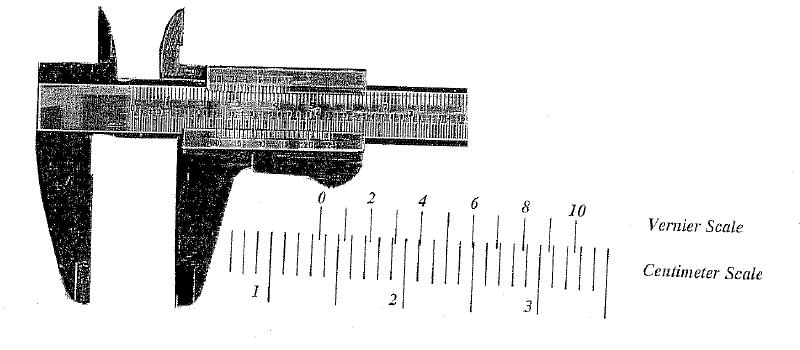
\includegraphics[width=6in]{vernier.JPG}
\vspace{-.25cm}
\caption{The Vernier Caliper:  The location of the zero on the vernier scale tells you where to read the centimeter scale (1.3 cm).  The vernier-scale line that lines up tells you the next digit (5).  This picture measures $1.35\pm 0.01 \unit{cm}$.}\label{f:vernier}
\end{center}
\begin{center}
\hspace{-2cm}
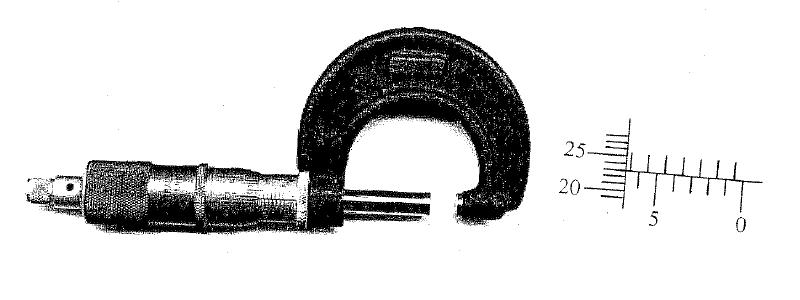
\includegraphics[width=6in]{micrometer.JPG}
\end{center}
\vspace{-.5cm}
\caption{The Micrometer Caliper:  Notice on the coarse scale, that the lower lines read (1, 2, 3, <ellipsis /> 6 in this picture) and the higher lines read the half-marks (0.5, 1.5, 2.5, <ellipsis /> 6.5 in this picture).  The location of the turning dial tells you where to read the coarse scale (6.5 mm).  The center line of the coarse scale tells you where to read the fine scale.  This is 23.0 (in units of $\times 10^{-2}$ mm), but not 23.5 and not 22.5 so the precision is 0.5 (in these units).  This measurement in mm reads $6.5 \unit{mm} + 0.230\unit{mm} = 6.730 \pm 0.005 \unit{mm}$. }\label{f:micrometer}
\vspace{-.5cm}
\end{figure}
%

%-------------------------------------------------------------------------------------
\onecolumn

\section{Standard Deviation}
\revised{Aug. 28, 2009}
\revision{Aug. 28, 2009}{Added Jack's picture back in}
\revision{Jan. 7, 1997}{Jack}

\subsection{Introduction}

Suppose you are standing in front of a dart-board.  You have a large number of darts and you throw the darts one at a time, trying to hit a 1 cm thick vertical line drawn on the dart-board.  Since you have a very good aim, let us say that 45\% of the darts hit the line.   This then means that you miss the line 55\% of the time; with a significant number of these misses being between .5 to 1.5 cm either to the left or to the right from the center of the line, and with a smaller number of misses being between 1.5 to 2.5 cm from the center line.

Is there some mathematical way of characterizing how good you are at this game?  What, for example, is the probability of missing the line by 1 cm?  The statistical analysis of random fluctuations in data can help answer these questions.   The word ``statistical'' implies that a relatively large set of similar measurements of a given physical quantity is available.  The random fluctuations in the data can be measured with the use of a mathematical term called the ``standard deviation.''

Suppose you collect data on a large number of throws, separating the data into categories (bins): The number of darts on the line, the number within .5 to 1.5 cm from the center, the number within 1.5 to 2.5 cm, etc.  A plot of this data with the dart positions on the x-axis and the number of darts hit within each bin plotted on the y-axis is called a histogram (see Figure~\ref{f:histogram}).  The envelope of this graphical data set is bell shaped, and is called a Gaussian or a Normal distribution curve.
%
\begin{figure}[bhtp]
\begin{center}
%\begin{picture}(400,200)
%\put(0,0){\line(0,1){200}}
%\put(0,0){\line(1,0){400}}
%\put(200,195){\vector(0,-1){25} $\mu$}
%\put(200,100){\vector(1,0){75}}
%\put(200,100){\vector(-1,0){75}}
%\put(200,105){$\sigma$}
%\end{picture}
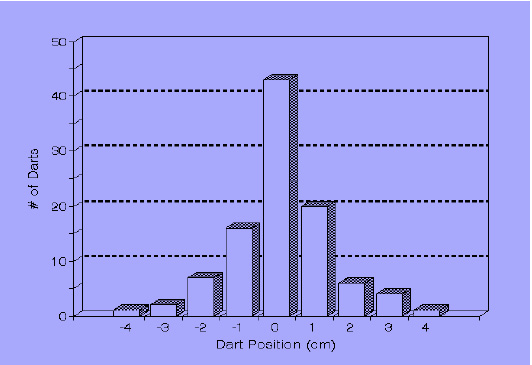
\includegraphics[height=2.5in]{darthistogram.jpg}
\caption{Histogram for the number of darts binned by distance from the centerline.}\label{f:histogram}
\end{center}
\end{figure}


The ``standard deviation'' is a measure of the spread or width of the histogram data.  A small standard deviation  means that there is a small spread in the data about the central mean value and implies that the data cluster closely about one value.   That is, there is a high degree of precision in the measurements.


The area beneath the curve, or below a part of the curve represents the probability of occurrence.  For example, the area beneath the curve between plus and minus one standard deviation from the mean represents a 68\% probability of your next throw falling within this range.  The area beneath the curve between plus and minus two standard deviations from the mean represents a 95\% probability of your next throw falling within this range.

In this experiment, you will study the use of the ``standard deviation'' in the statistical analysis and probability involved with flipping pennies.
\subsection{Experimental Purpose}

The goal of the experiment is to determine how the mean, standard deviation, and standard deviation of the mean depend on the amount of data (number of samples) taken.  You should also consider how well the data fit to a normal distribution.

\subsection{Student Outcome}

In this experiment, you should learn
\begin{enumerate}
\item the formulas for and the roles of the mean, the standard deviation, and the standard deviation of the mean in the statistical analysis of data containing random errors,
\item how to create histograms and scatter plots,
\item how to include trendlines on scatter plots, and
\item why more data is always better.
\end{enumerate}

\subsection{Pre-Lab Work}
\begin{lablist}
\item Define the following, both in a sentence and with a mathematical formula:  mean, standard deviation (sometimes called the standard deviation of a single observation), and standard deviation of the mean.  Be sure to describe the difference between these two terms.
\item Define the following:  histogram, probability, \& probability distribution (Normal distribution).
\item What does the total area under the Normal distribution curve represent?
\item How should the axes of the histogram of the data you will take for this lab be labeled?  Give a very specific scale for the x-axis.  (Hint: Read the procedure below.)
\item Make a sketch of an inverse function, like $y=1/x$.
\end{lablist}

%\twocolumn[\vspace{-.5cm}
\subsection{Experimental Procedure}

Each individual will receive 20 pennies and will then simultaneously toss all of the pennies.  Count the number of heads, and repeat 25 times.   Each individual will then have collected 25 pieces of data.
%\\]

\subsection{Analysis}

\begin{lablist}
\item Calculate the mean, the standard deviation  and the standard deviation of the mean for your first ten tosses and for all 25 tosses.  Show your calculations.
\item Make a histogram plot (by hand in your note book) for your 25 tosses.   On this histogram superimpose a sketch of your best guess of the corresponding Normal distribution curve.
\item How well does your data fit a normal distribution curve?  Explain the reasons for any large discrepancies.
\item Obtain histograms and calculations of the mean, the standard deviation and the standard deviation of the mean for the following data sets:  i) your lab group,  ii) about 1/2 of the class, and iii) the entire class.   These histograms can be obtained with the use of a computer program, provided by the instructor.
\item Draw graphs of:  the mean, the standard deviation, the standard deviation of the mean, versus the number of data entries.   Use the standard deviation of the mean  as the error bars for both the mean and the standard deviation,  draw these error bars on these two graphs.
\item Describe how the values of the mean, the standard deviation, and the standard deviation of the mean, change as the number of data items in the set increases.  What does this infer about the accuracy and about the precision of the data as more and more observations are made?
\item Show that the standard deviation of the mean varies inversely as the square root of the number of data items in the sample.   How well does the data in this lab agree with this prediction?   (Make a graph of the standard deviation of the mean versus the square root of the number of data items in the sample.)
\end{lablist}

\subsection{Questions}
\begin{enumerate}
\item What is the probability of flipping the 20 pennies and getting 5 heads, or 8 heads, or 10 heads, or 15 heads?   Answer this question by analyzing your data, the entire class' data and the normal distribution curve fit to your data.  Explain any differences between these sets.
\item What percentage of your individual readings fall within plus or minus one standard deviation,  two standard deviations?   Compare your answer to the theoretical answer from a normal distribution curve.  What are the percentages for the class data?
\item Does the height of the histograms change as a function of the number of trials?  If so, how?
\item How does the width at 1/2 the maximum height for the histograms change as a function of the number of trials?  Label this width on your histograms.  Is this width a reasonable estimate of the standard deviation?
\item Does the standard deviation of a single observation and/or does the standard deviation of the mean change significantly as the number of tosses increase?  What does this infer about the accuracy and about the precision of the data as more and more observations are made?
\end{enumerate}

\subsection*{Resource Materials}

Meyer, \underline{Data Analysis for Scientists and Engineers} John Wiley, (1975) p.19-48, 223-253


%-------------------------------------------------------------------------------------
\onecolumn

<chapter><title>Constant Acceleration</title>
<!-- Revisions
\revised{Sept. 14, 2015}
\revision{Sept. 14, 2015}{Commented out Graphs and Tracks.  Updated Pasco Reference from DataStudio to Capstone}
\revision{Sept. 16, 2008}{Created?}
-->

    <objectives><title>Experimental Purpose</title>
    <introduction><p>Using position versus time and velocity versus time graphs, verify that the equations of constant acceleration accurately describes the behavior of objects under constant acceleration and that it is possible to distinguish acceleration due to gravity from acceleration due to friction.</p>
    </introduction>
    </objectives>

    <section><title>Student Outcomes</title>
    <p>In this exercise, the student should develop an understanding of the relationships between the position and the instantaneous velocity of an object, as well as how each of these can vary as functions of time.   We will only consider the special case where the object experiences constant acceleration.</p>

    </section>

    <section><title>Materials</title>
    <p>An aluminum track, a low-friction cart, computer interface with PASCO Capstone<m>^{\rm tm}</m> software, a sonic motion sensor, a small steel ball.</p>
    </section>

    <section><title>Procedure (to be paired with Section~\ref{ss:AccAnalysis})</title>

    <subsection><title>Cart and Flat Track</title>\label{sss:FlatTrack}
    <p>Log into the computer (so you can save your data to your network drive) and then open Pasco Capstone.
    (Section~\ref{s:Capstone} will provide some instructions for setting up the software and connecting the equipment.)
Connect the motion sensor to the computer interface.
Set the data rate of the motion sensor at <m>50 \unit{Hz}</m>.
Place a steel ball on the track and adjust the leveling screw at one end of the track to see if the ball rolls one way or the other.  This will roughly level your track.
Place the sensor about 20 cm from the end of the track, because this is the minimum distance detected by the sensor.  (You might need to use the <q>sail</q> for the sensor to see the cart.)</p>

    <p>Place the cart on the track.  Capstone, via the sonic ranger, can measure the position and velocity of the cart as a function of time.  (This is explained in Section~\ref{s:Capstone}.)
<ol>
<li><p> Assume the track is frictionless and predict how the cart will move if the track is not perfectly level; include a comment about how the velocity versus time graph will look when it goes uphill versus when it goes downhill.  Should these be the same?
</p></li> <li><p> What do you expect the graph to look like if the track <em>is</em> perfectly level?  Will it be the same going left versus going right?
</p></li> <li><p> Now, assuming it is perfectly level, what will friction do to the motion?  How do you expect this to affect the graphs?
</p></li> </ol>
\setcounter{dave}{\theenumi}
</p>

    <p>We will take four sets of data: a slow, constant velocity towards the ranger; a slow, constant velocity away from the ranger; a faster, constant velocity towards the ranger; and a faster, constant velocity away from the ranger.  The two slow speeds should be about the same and the two faster speeds should be about the same.  For each case, start the sonic ranger and then bump the cart firmly, but not violently(!).</p>

    <p>On Capstone, you should have four curves of velocity versus time.  Fit each with a trendline and display the equation of the trendline on the screen.  Interpret the coefficients (slope and intercept) by noting their units, values, and uncertainties.  You should also print out (in landscape mode) the position versus time graph, the velocity versus time graph, and the acceleration versus time graph.  (You should notice that the acceleration versus time graph is <em>very</em> noisy.)</p>

    </subsection>
    <subsection><title>Cart and Sloped Track</title>\label{sss:SlopedTrack}
    <p>Place a small block under one end of the track, so that the track is now tilted at a small angle with the sensor at the top of the incline.  Measure the angle using a protractor or calculate it by measuring the two legs of the triangle and using the inverse sine.  (Be careful about measuring the height.)</p>

    <p.>We will consider <em>three cases</em> for the sloped track: <em>First</em>, allow the cart to roll (without an initial push) down the ramp.  <em>Second</em>, gently push the cart down the ramp.  DON'T let it fly off or crash into anything.
<ol>
\setcounter{enumi}{\thedave}
<li><p> Should these two cases have the same acceleration while rolling down the ramp?  How will that affect the shape of the velocity versus time graphs?
</p></li> <li><p> Should these have the same initial velocity?  How will that affect the graphs?
</p></li> </ol>
\setcounter{dave}{\theenumi}
In the <em>third</em> case, start the cart at the bottom of the incline and roll it up the ramp, allowing it to roll back down on its own.  Push it hard enough to get mostly up the ramp, but not so hard that it hits the sonic ranger.
<ol>
\setcounter{enumi}{\thedave}
<li><p> Should this case have the same acceleration while it goes up the ramp as while it goes down the ramp? How can we see that on the velocity versus time graphs?
</p></li> <li><p> Should this case have the same acceleration (either while it goes up the ramp or while it goes down the ramp) as the previous two cases of rolling down the ramp?
</p></li> </ol>
\setcounter{dave}{\theenumi}
</p>

    <p>In Capstone, you should be able to display all three graphs (position v time, velocity v time, and acceleration v time).  You should also be able to display all three cases of data on each of these graphs.  On the velocity versus time graph, fit each of the three graphs with a linear trendline.  The next section will ask you to analyze how well the data match up to these lines.  (It might be interesting to also fit the position vs time curves to parabolas.  Be sure to print out copies of your three graphs.</p>

    <p>Your lab should note the following results and explain their meaning:  slope and y-intercept, the uncertainties (precision) in both the slope and intercept, and the <m>r</m> value (correlation coefficient). </p>

    </subsection>
    </section>

    <section><title>Further Analysis and Discussion</title>\label{ss:AccAnalysis}

    <subsection><title>Cart and Flat Track</title>

    <p>Based on the results of Sec.~\ref{sss:FlatTrack}, write a short analysis of the relationship between these two graphs (x and v versus time).   From the velocity versus time graph (specifically from the trendline) determine the value of the acceleration of the cart down the track; be sure to include the uncertainty of the acceleration and the units.
<ol>
<li><p> Do you see any evidence that the track was not perfectly level?
</p></li> <li><p> Do you see any evidence that there is any friction as the cart moves along the track?
</p></li> <li><p> What does the intercept of the velocity versus time graph tell you?
</p></li> <li><p> If the slopes are different, then discuss any pattern that you see.  If the slopes are (essentially) the same, then find an average and a standard deviation of the four values.
</p></li> <li><p> Does it matter how fast the cart travels?
</p></li> </ol>
\setcounter{dave}{\theenumi}
    Discuss any evidence observed in your data when answering these questions.  Also consider the magnitude of the uncertainties when writing your conclusions.</p>

    </subsection>
    <subsection><title>Cart and Sloped Track</title>

    <p>Based on the results of Sec.~\ref{sss:SlopedTrack}, write an analysis of the relationship between the two graphs
(x and v versus time).  From the velocity versus time graph determine the value of the acceleration of the cart down the track.
<ol>
\setcounter{enumi}{\thedave}
<li><p> For the two downhill cases, use your uncertainty analysis to determine if the acceleration of the cart changed when it was given a small push.
%</p></li> <li><p> For the case that you copied into Excel, compare the results for the acceleration (with uncertainties) between <q>Data Studio</q> and Excel.  Comment on any differences.
</p></li> <li><p> Is there an accuracy<fn>If the track were frictionless, then the acceleration should be <m>a=(9.81\unitfrac{m}{s^2})(\sin\theta)</m>, where <m>\theta</m> is the angle that the incline makes.</fn> that can be computed for this part of the experiment?
</p></li> </ol>
\setcounter{dave}{\theenumi}
%
Inspect the line/curve that is defined by the data on the Distance traveled vs. time graph.
<ol>
\setcounter{enumi}{\thedave}
<li><p> What is its shape?  Is the shape of the graph what you would expect for constant acceleration (straight line, parabola, etc.)?  Explain your reasoning.
</p></li> <li><p> Consider the trendline that you added.  Does/should the trendline line go through the origin?  What is the value of y-intercept of the X vs T graph?  What physical quantity does the intercept represent?  Explain why it has that value.  Hint: (Think about where the sensor was located.)
</p></li> <li><p> What does the slope (whether it's constant or not) of the line on this graph signify?
</p></li> </ol>
\setcounter{dave}{\theenumi}
Now consider the Instantaneous Velocity  vs. Time graph.
<ol>
\setcounter{enumi}{\thedave}
<li><p> Does the curve/line on this graph have the shape you would expect for an object undergoing constant acceleration? Explain.
</p></li> <li><p> What was the value of the y intercept on this graph (include units and uncertainty!)?  Explain its significance.  To what does it refer?  Think carefully about what you plotted on the X-axis!
</p></li> </ol>
    </p>

    </subsection>
    </section>
</chapter>

%-------------------------------------------------------------------------------------
\onecolumn

<chapter><title>Newton's <m>2^{\rm nd}</m> Law on a Linear Track with the Sonic Ranger</title>\label{s:Newton}
<!-- Revisions
\revised{Sept. 14, 2015}
\revision{Sept. 14, 2015}{Updated Pasco Reference from DataStudio to Capstone}
\revision{Sept.~23, 2008}{}
-->

<introduction><title></title>Introduction to Forces}

Forces are related to the natural motion of bodies, where one object can affect the motion of another object.  That is, forces are interactions between objects affecting their motion.  Although the famous Greek philosopher Aristotle claimed that a force was necessary to <em>maintain</em> any motion, careful analysis by Italian physicist Galileo Galilei in the mid-<m>17^{\rm th}</m> century and by Sir Isaac Newton, a British mathematician and physicist (1642-1727), eventually distinguished the effects of friction and allowed Newton to create a mathematically consistent theory of motion.  These concepts were published in Newton's book <q>Mathematical Principles of Natural Philosophy</q> in 1687, for which (among other accomplishments) Newton is regarded as one of the greatest scientists of all time.

All forces can be placed in one of two main categories.  First, there are natural (or fundamental) forces like the gravitational force, the electromagnetic force, or the nuclear forces.  The gravitational force is a force on a body by another body (like the Earth), this force is an interaction between their two masses.  The electromagnetic force is an interaction between the charges of two bodies.  These forces may act on an object without any direct physical contact between the two bodies.  This type of force is sometimes called an <q>action at a distance</q> force.  All other forces are in a second category called <q>contact forces.</q>

<subsection><title></title>Newton's First law}

<quote>
If there are no forces acting, then objects will remain at rest or, if not at rest, will maintain their velocity.
</quote>
If this is true, then we can study the forces acting on a body based on the motion of the body, specifically through the change in the velocity of an object.

</subsection>
<subsection><title></title>Newton's Second Law}

Not only is a force necessary to change the motion (to cause an acceleration), the amount of acceleration that a force causes is predictable and is inversely proportional to the mass.  The same sized force causes a small mass to accelerate a lot and a large mass to accelerate a little.  this is expressed by the equation:
<me> \vec F_{\rm net} = m \vec a. </me>
The net force, <m>\vec F_{\rm net}</m>, is the vector sum of all forces acting on an object.  If we have an extended object (such as a weight hanging off of a table, but connected to a cart that is on the table), then we need only consider forces that are <q>external</q> to the system:  So long as both objects accelerate at the same rate, we do not need to consider the <q>internal</q> tension that the string exerts between the connected bodies.

</subsection>
<subsection><title></title>Newton's Third Law}

Inherent in the description of a force is that it is an interaction between objects: there must always be two objects that interact.  These objects exert equal and opposite forces on each other.  That is,
<quote>
If there is a force exerted on object 1 by object 2, then there is necessarily and simultaneously a force exerted on object 2 by object 1 that is equal (in magnitude) and opposite (in direction) to the original force.
</quote>
Remember that these two forces are on different objects and that the two bodies in direct contact exert forces on each other.  Remember then that if there is contact between the object (any part of the system) and anything else then there is an outside force on the object (system) and that if there is no contact (the two bodies break contact) then there is no force.


</subsection>
</introduction>
    <objectives><title>Experimental Objective</title>

    <introduction><p>In this experiment, we will assume that the first law is true and focus on the second law.
    By measuring (a) the velocity versus time for a cart being pulled down a track and (b) the applied force that is pulling it, we can plot the acceleration versus the force and verify the validity of Newton's second law of motion: <m>\vec F_{\rm net} = m \vec a</m>.</p>
    </introduction>
    </objectives>

</section><section><title></title>The Experimental Setup}

<ul>
<li><p> A low-friction linear cart and track will be used, this reduces the friction between the cart and the track.
</p></li> <li><p> A string will be connected to the cart and a known mass will be hanging from the end of the string (and over a pulley).   The hanging mass will exert a constant horizontal force on the cart as the mass falls all the way to the floor.  This gives a constant acceleration to the cart.
</p></li> <li><p> The sonic motion sensor will be used to measure the position of the cart as a function of time.
</p></li> <li><p> The carts and tracks need to be handled with care.  Scratches can add friction to the system.
</p></li> </ul>

</section><section><title></title>Pre-Lab Work}

<ul>
<li><p> Draw a free-body force diagram for the cart and for the hanging mass.
</p></li> <li><p> Derive an equation for the acceleration of the system, in terms of, the mass of the cart and the hanging body.
</p></li> </ul>

</section><section><title></title>Procedure}

<ul>
<li><p> If the cart is given an initial push (without the hanging mass and string attached) then the cart should travel with a constant velocity down the horizontal track, if there are no other forces acting on the cart.  Carry out  a couple of constant velocity runs on the track, to check for the effects of friction and to see how level the track is. The track may need a level adjustment.  Do runs in both directions.  Maybe the track can be tilted so that the friction is countered by the tilt of the track.
</p></li> <li><p> Connect a string to the cart and run it through the hole at the end of the track, then over a pulley.  Make sure that the string is horizontal.  Measure the height of the string at both ends of the track, to see if the string is horizontal.
</p></li> <li><p> The hanging mass should be much less than the mass of the cart.  Use a small plastic cup to hold the hanging masses.   Measure the mass of  this cup.  The total mass of the system must be kept constant for all parts of the experiment.   The hanging mass and the mass of the cart should vary, but their total must be kept constant, by moving small mass amounts from the cart to the hanging cup.  Record the mass of the cart, the hanging cup mass, and the extra masses which are to be transferred from the cart to the cup.
</p></li> <li><p> Take data with Capstone and the motion sensor as the cart travels with constant acceleration down the track.   Determine the acceleration of the cart from a linear regression using the velocity vs time data (a linear fit line in Capstone).  Record the acceleration value and its uncertainty.
</p></li> <li><p> Collect  7 data runs, where about 5 grams is transferred each time from the cart to the hanging mass.   Determine the acceleration of the cart (and the uncertainty for the acceleration) for each of these 7 runs.
</p></li> </ul>

</section><section><title></title>Analysis}

<ul>
<li><p> Make a graph of the acceleration of the system (y-axis) versus the weight (<m>mg</m>) of the hanging body (x-axis),  should include 7 data points.    Do this in Excel.   Carry out a linear regression for this data set.   Quote the  slope and intercept values, their uncertainties, their p-values, and the <m>R^2</m> value.     Show a sample error bar (on the graph) for at least one of the points of this graph.
</p></li> <li><p> Derive (show it completely)  an equation for the acceleration of the system versus the weight of the hanging body.  Plot this theory equation on your graph (as a second series, a line but no points).
</p></li> <li><p> Compare your graph to the predicted theoretical equation, that is compare the values of the slopes and intercepts.  What is the physical significance of the slope and of the intercept from the graph?  That is, what physical quantity does the slope of this graph equal?
</p></li> <li><p> In many mechanics experiments, there may be deviations from the expected or theoretical results because of the effects of friction.  Frictional forces are sometimes difficult to take into consideration.  If there are deviations between your results and the predicted theory then try to distinguish whether they are caused by a tilt of the track, friction between the cart and the track or the friction between the string and the pulley.  What might be expected in the results from these different systematic effects?    That is, would the slope be expected to increase or decrease slightly because of the effects of friction?
</p></li> <li><p> When designing experiments, it is important to keep control parameters; in this case a parameter which is kept constant.   What parameter held this role in this experiment?
</p></li></ul>

%\vfill\hfill(<m>\hookrightarrow</m>)
%\onecolumn
</section><section><title></title>Questions}

<ol>
<li><p> Why is it important to keep the total mass of the system constant?   What would happen if the total mass of the system was not held constant?    If one simply added mass to the hanger without keeping the system's mass constant,  how would their data appear on the graph of the acceleration vs <m>mg</m>?
</p></li> <li><p> What would happen if the track was not level?   If the beginning end of the track is higher,  how would the acceleration of the system be affected?
</p></li> <li><p> If your group has a discrepancy between the results and the theory, could friction be used to explain your results?   Explain how.   In this case, how much of a tilt in the air track would be needed to explain the discrepancy?   Show this calculation.
</p></li> <li><p> What would happen to the cart's acceleration if the cart was given an initial push?
</p></li> <li><p> What are the two greatest sources of uncertainty in this experiment?   Are they random or systematic errors?   Be specific and quantify your answer.
</p></li> </ol>


</chapter>

%-------------------------------------------------------------------------------------
\onecolumn

<chapter><title>Dry Sliding Friction</title>
<!-- Revisions
\revised{Sept.~28, 2015}
\revision{Sept.~28, 2015}{}
\revision{Sept.~23, 2008}{}
-->

<introduction><title></title>Introduction}

Friction is a force which retards the relative motion of any body while sliding over another body.  The frictional force acting on a body is parallel to the surface that the object is sliding upon and it is directed opposite to the direction of motion.  The phenomenon of friction is rather complicated, especially at the microscopic level, because it is dependent on the nature of the materials of both contacting surfaces.  The frictional force depends on the roughness or the irregularities of both surfaces.  At the macroscopic level, the nature of this force can be described by a simple empirical law, first given by Leonardo da Vinci:
<quote>
The magnitude of the force of friction between unlubricated, dry surfaces sliding one over the other is proportional to the normal force pressing the surfaces together and is independent of the (macroscopic) area of contact and of the relative speed.
</quote>
At the microscopic level, the frictional force <m>(F_f)</m> does depend on the actual area of contact of the irregularities of the surfaces.  This actual area of contact then increases as the force pressing the two surfaces together increases, this force is called the load.  Using Newton's <m>2^{\rm nd}</m> Law in this perpendicular direction we can conclude that the magnitude of the load is equal to the Normal force <m>(F_N)</m> of the surface pushing on the object.  Therefore we may write that
%
<me>
F_f \propto F_N
\mbox{\ \ \ \ or \ \ \ \ }
F_f = \mu F_N
</me>
%
where the Greek letter <m>\mu</m> (<q>mew</q>) is a dimensionless constant of proportionality called the coefficient of friction.

When a body is pushed or pulled parallel to the surface of contact and no motion occurs, we can conclude that the force of the push or pull is equal to the frictional force, using Newton's <m>2^{\rm nd}</m> Law of motion.  As the applied force is increased, the frictional force remains equal to the applied force until motion results.  At this maximum value of the applied force, the frictional force is also a maximum and is given by
%
<me>
F_f = \mu_s F_N
</me>
%
where the subscript <m>s</m> stands for static (non-moving) friction.  This equation can only be used at this maximum static point also called the point of impending motion.  At the instant that the applied force becomes greater than the maximum fs, the body is set into motion and this motion is opposed by a frictional force called the kinetic (sliding) frictional force and is given by
%
<me>
F_f = \mu_k F_N
</me>
%
where the subscript <m>k</m> stands for the kinetic (moving) friction.  In general, <m>\mu_k < \mu_s</m>; that is, it takes more force to overcome the static friction than to over come the kinetic friction.  The coefficients of friction are generally less than one, but may be greater than one, and they depend on the nature of both surfaces.



	Consider a system comprised of a block on a horizontal surface being pulled horizontally by a string connected to a hanging weight.   Assume that the system is accelerating with a constant acceleration.  Then the <m>\mu_k</m> can be solved for by the following equation:
%
<me>
\mu_k  = \frac{ mg - (M+m) a }{ Mg},
</me>
where <m>M</m> is the mass of the block and <m>m</m> is the hanging mass.


    </introduction>
    <objectives><title>Experimental Objective</title>

    <introduction><p>In this experiment you will devise methods to investigate the nature of both the frictional force and the coefficient of friction, and to test the validity of da Vinci's empirical rule.</p>
    </introduction>
    </objectives>

<section><title></title>Pre-Lab Analysis}

<ul>
<li><p> Draw force diagrams for the following case:     a block on a horizontal surface pulled by a hanging mass and a string  (include the friction force).
</p></li> <li><p> Write out the corresponding Newton's <m>2^{\rm nd}</m> Law equations for forces both parallel and perpendicular to the contact surface.
</p></li> <li><p> Derive the relevant equations for each of the above two cases for which the coefficients of friction can be determined:
    <ul>
    <li><p> Case one is static, but at the point of motion.
    </p></li> <li><p> Case two is the kinetic case.
    </p></li> </ul>
</p></li> </ul>


</section><section><title></title>The Experiment}

For the block on the horizontal plane:	
<ol>
<li><p> Clean the block and the plane, so that they are free of dust and other contaminants.  \\
Make sure the track is level, as in previous labs.
</p></li> </ol>
\setcounter{dave}{\theenumi}

</subsection><subsection><title></title>Break Static Friction - pull until moves}\label{sss:staticfriction}
<ol>
\setcounter{enumi}{\thedave}
<li><p> Set up the Dynamics Track, cart, force transducer and friction block.  The force transducer attaches to the dynamics cart, the friction block rests on the track (felt side down).
</p></li> <li><p>\label{i:staticpull} Attach a string to the force transducer.  The force transducer needs to be zeroed before data collection starts.  Collect data, and slowly start pulling on the string (<em>be sure to pull the string horizontally</em>) and slowly increase the pull force until the cart is moving down the track. Using just the maximum force (at the point of impending motion) the coefficient of static friction can be calculated.
</p></li> <li><p>\label{i:statictest} Test the relationship between the force of friction and the normal force, by changing the load force (normal force) and measuring the force of friction at the point of motion impending. Carry this out for a total of five data points.  Graph the frictional force versus the normal force.  Calculate the coefficient of static friction from this graph.
</p></li> </ol>
\setcounter{dave}{\theenumi}

</subsection><subsection><title></title>Effect of Surface Area - distinguish pressure from force}\label{sss:friction-area}

Consider pushing a pencil into your arm. (Well, don't <em>actually</em> do it!)  If you use the erasure end, then you can feel the force, but it doesn't hurt.  If you use the sharpened tip with the <em>same</em> force then it will certainly hurt!  So, you have the idea that the same force spread over a different surface area <em>can</em> have a different effect; but it doesn't <em>always</em> have a different effect.  For this part of the lab, you will test the relationship between the coefficient of friction and the macroscopic area of contact between the block and the surface.
<ol>
\setcounter{enumi}{\thedave}
<li><p> Place the friction block on its side (felt side down) and repeat Steps~\ref{i:staticpull} and~\ref{i:statictest} for three (rather than five) of the previous load forces.
</p></li> <li><p> Add the plot of this <m>F_f</m> versus <m>F_N</m> as a new series to the graph of Part~\ref{sss:staticfriction}.
</p></li> </ol>
\setcounter{dave}{\theenumi}

</subsection><subsection><title></title>Friction while Accelerating}

<ol>
\setcounter{enumi}{\thedave}
<li><p> Apply a force (hanging mass, pulley, and string) large enough to accelerate the block. Use the Sonic Ranger to collect data.
</p></li> <li><p> Graph the velocity vs time.  Determine the acceleration of the block from the slope of the line.
</p></li> <li><p> Repeat this part four or five times with a different normal forces.  (You may use any hanging mass.)
</p></li> <li><p> Add the plot of this <m>F_f</m> versus <m>F_N</m> as a new series to the graph of Parts~\ref{sss:staticfriction} and~\ref{sss:friction-area}.
</p></li> <li><p> Calculate the coefficient of kinetic friction from the slope.
</p></li> </ol>



</section><section><title></title>Analysis}
<ul>
<li><p> The experimental precision should be estimated for all parts of this experiment and care should be taken for all of the measurements, but it is more important to investigate the relationships than it is to repeat the experiment many times or to try to achieve high precision in the data.
</p></li> <li><p> Explain why the normal force on the block by the surface rather than the weight of the object is related to the frictional force.
</p></li> <li><p> Interpret the slope and intercept of the graphs.
</p></li> <li><p> Compare the slopes from each of the three parts.  Decide which should be the same and which should be different.
</p></li> <li><p> Calculate the \% decrease of the static to kinetic coefficient of friction.
</p></li> <li><p> Comment on the validity of the empirical rules of friction.
</p></li> </ul>


</section><section><title></title>Questions}

For all questions, and when possible, use your experimental or theoretical results to demonstrate your answers to the questions.
<ol>
<li><p> Does the coefficient of friction depend on the area of contact?
</p></li> <li><p> Does the coefficient of friction depend on the mass of the object?
</p></li> <li><p> Does the coefficient of friction depend on the normal force of the object?
</p></li> <li><p> Does the frictional force depend on the normal force of the object?
</p></li> <li><p> Does the coefficient of kinetic friction depend on the speed of travel?
</p></li> <li><p> When the object was pulled by a string, how would the forces be affected if the cord was not horizontal?
</p></li> <li><p> What would happen to the coefficient of friction if the surfaces were lubricated with oil?
</p></li> </ol>


</chapter>

%-------------------------------------------------------------------------------------


\onecolumn
<chapter><title>Centripetal Force</title>
<!-- Revisions
\revised{Fall 2006}
-->
<introduction><title></title>Introduction}

We will be investigating the force which is necessary to maintain the circular
motion of an object.
The apparatus used will allow you to spin an F-shaped arm which has a mass
suspended from the
top arm.  This mass will be held in place by a spring which makes up the lower
arm.  The spring
will provide the centripetal force.  You will need to be familiar with the
ideas of circular motion,
centripetal versus centrifugal force, centripetal acceleration, and angular
velocity.  In addition to
these concepts, try to understand how we will measure the angular speed in lab.

The centripetal acceleration <m>a_c</m> is calculated from the following equation
written either <m>\displaystyle a_c=\frac{v^2}{r}</m> or <m>\displaystyle a_c =
\omega^2 r</m>
where <m>v</m> is the linear velocity of the particle, <m>\omega</m> is the
angular velocity, and <m>r</m> is the radius of the circle.  Note that angular
velocity is measured in radians per second.

From Newton's second law, <m>\vec F = m \vec a</m>.
Therefore, the force required to keep the particle of mass <m>m</m> moving in a
circle
with constant speed is
%
<me> F = ma_c = \frac{mv^2}{r} = m\omega^2r </me>
%
Recall that the centripetal force is not a force applied <em>in addition</em> to
other existing forces.
The centripetal force is <em>whatever combination</em> of existing force act to
maintain circular motion.

    </introduction>
    <objectives><title>Purpose</title>

    <p>It is our purpose to verify the above equation experimentally by measuring the applied force
and comparing it to the specific combination of variables expressed as either
<m>\frac{mv^2}{r}</m> or <m>m\omega^2r</m>.</p>
    </introduction>
    </objectives>

<section><title></title>Pre-Lab}

<ol>
<li><p> Why do we say that an object moving with <em>constant speed</em> in a
circular path is being accelerated?
</p></li> <li><p> In which direction is that acceleration?  How do you know?
</p></li> <li><p> Is this <m>a_c</m> <q>centripetal</q> or <q>centrifugal?</q>
</p></li> </ol>

</section><section><title></title>The Experiment}

The centripetal force is supplied by a spring.  Since we cannot directly
measure <q>the
force exerted by the spring while it is rotating</q> while it is rotating,
determine how
we can measure <q>the force exerted by the spring during the
rotation</q>
when the spring is not rotating.

<ul>
<li><p>\label{i:r} By means of the lab apparatus, a mass <m>m</m> can be made to rotate with a constant (and measurable) angular speed <m>\omega</m>.  With some practice, it is possible to adjust the speed so that the radius of the path remains constant.  The value of the radius, <m>r</m>, is marked on the apparatus and so can be measured easily.
</p></li> <li><p>\label{i:m} Measuring the mass should be an obvious task.
</p></li> <li><p>\label{i:w} Measuring the angular speed <m>\omega</m> is straightforward, but may not be obvious.  To do so, consider the following:
    <ul>
    <li><p> Angular speed <m>(\omega)</m> is measured in <m>^{\rm radians}\!\!/_{\!\rm second}</m>.
    </p></li> <li><p> <m>\omega</m> is related to the rotational speed which is measured in <m>^{\rm revolutions}\!\!/_{\!\rm second}</m>.
    </p></li> <li><p> There are <m>2\pi</m> radians in 1 revolution.
    </p></li> <li><p> We can count the number of revolutions.
    </p></li> <li><p> The <q>period of rotation,</q> <m>T</m>, is defined as the number of seconds per revolution.
    </p></li> <li><p> We measure the period not by timing a single revolution, but by measuring the time for multiple (20) revolutions divided by the number of revolutions. (This averages out any uncertainty due to reaction-time.)
    </p></li> </ul>
</p></li> <li><p>[] As the mass rotates, its period of rotation can be measured.  This allows you to calculate the angular speed using the hints above.
</p></li> <li><p> Repeat the entire procedure for a second value of r.
</p></li> </ul>

</section><section><title></title>Analysis}

From measurements of <m>m</m>, <m>\omega</m>, and <m>r</m>, calculate the theoretical centripetal force on
the mass (which experimentally is supplied by the spring).  The (unmeasurable) amount
of force exerted by the spring to hold the spinning mass at a particular radius is
equal to the (measurable) force required to stretch the spring to that radius.  Experimentally determine
the force necessary to stretch the spring to a specific radius and compare that with the amount
of centripetal force calculated above.
</chapter>

%-------------------------------------------------------------------------------------

\newpage

<chapter><title>Conservation of Energy on a Linear Track</title>
<!-- Revisions
\revised{October 24, 2015}
\revision{October 24, 2015}{made it a one week lab}
\revision{August 24, 2009}{}
-->

<introduction><title>Introduction</title>

Conservation laws play a very important role in our understanding of our physical world.  For example, the law of conservation of energy can be applied in all physical processes.  This is a fundamental and independent statement about the nature of the physical world.  It is not necessarily derivable from other laws like Newton's Laws of motion.  Though for simple point mass systems, the law of conservation of energy can be derived from Newton's Laws.  It can be shown that the net work done on a system is equal to the change in the kinetic energy <m>(W_{\rm net} = \Delta K)</m> of the system; this is called the work-energy theorem and it can be written in a variety of forms.  When a net positive work is done on a system, the kinetic energy of the system increases, and when a net negative work is done on the system (as from a friction force), the kinetic energy of the system decreases.

When the gravitational force acts on a system, the work it does on the system, <m>W_g</m>, is the gravitational force <m>(mg)</m> times the vertical displacement <m>(h=\Delta y)</m>: <m>W_g=mg\Delta y</m>.  For convenience, this is called the change in gravitational potential energy <m>(W_g = - \Delta P)</m>.  <em>If</em> the gravitational force is the only force acting on the system then <m>W_g = W_{\rm net}</m> and therefore, <m>-\Delta P = \Delta K</m> for the system.  When a force can be associated with a potential energy, it is called a <q>conservative force.</q>  Another kind of potential energy deals with an elastic potential energy, like in a spring.  The energy stored in a spring is given by the formula <m>P_s = \frac{1}{2} k \Delta x^2</m>.

<em>If</em>, on the other hand, a force dissipates energy, then it is called a <q>nonconservative force</q> and it will have no associated potential energy.  Frictional forces are an example of a nonconservative force and the work done by a frictional force is negative because (physically) the frictional force removes energy from the system and (mathematically) the frictional force and the displacement are in opposite directions.  This work done by friction is converted into heat or sound.  To distinguish the energy of heat or sound from the potential and kinetic energy, we define the total mechanical energy, <m>E=K+P</m> at any point.  Since frictional forces remove mechanical energy, we say <m>W_f = \Delta E = \Delta K + \Delta P</m>.

In general then, the law of conservation of energy states that energy can not be created or destroyed, but can only change from one form to another; or the total energy of the system at point A is equal to the total energy of the system at point B.

    </introduction>
    <objectives><title>Experimental Objective</title>

    <introduction><p>The purpose of this experiment will be to verify the validity of the law of conservation of mechanical energy, that <m>\Delta E = 0</m> as a cart runs along a track.</p>
    </introduction>
    </objectives>

</section><section><title></title>The Experiment}

We would like for you to verify the conservation of mechanical energy in two different situations; so, there are two parts to this experiment.
We will first consider a flat track with accelerated motion, as in the Newton's Law lab and the Friction lab.  We can then consider an inclined plane.  You will not be given an explicit procedure, but rather you will be given a series of questions with answers that will imply the procedure.  Part of the experiment is for you to figure out for yourself what the best course of action is.  Please answer the questions as they are asked.

%There is enough analysis for this lab that you will have two weeks to complete the lab.  During the first week, you will do the two parts of the experiment and begin to write up your report.  During the second week, you will do some analysis and re-run the experiment to determine the cause of differences from expectations.  A single lab report will be due after the second week of experimentation.

</subsection><subsection><title></title>Flat Track}\label{sss:1flat}

Set up the dynamics cart on a horizontal dynamics track.  Set up the motion sensor at one end of the track and a pulley at the other end so that the pulley partly extends past the edge of the table.  Hang the basket over the pulley so that it can accelerate the cart along the track -- you might need extra weight in the cart to keep it from accelerating too fast.  In order to use this motion to verify the validity of the conservation of mechanical energy, we need to measure some variables.  Answer Questions~\ref{q:1KE} and~\ref{q:1PE} to decide on the relevant variables.  Question~\ref{q1:2or1} should help you determine how to finish setting up the equipment.

Once you decide what variables to measure, run the experiment for one set of masses while measuring the appropriate variables.  Put the data into Excel and decide what plot(s) will allow you to verify the validity of the conservation of mechanical energy.  Question~\ref{q:1plots} may help with this.  Decide if you need a trendline.  Relate the information in Question~\ref{q:1EKP} to the statement you are trying to verify.

%Save your data so that you can do further analysis next week.

</subsection><subsection><title></title>Sloped Track}\label{sss:1sloped}

Remove the pulley from the track.  Your cart will have either a spring-loaded <q>battering ram</q> on the front or a pair of magnets.  If you have the battering ram, then you will want the end of the track with the rubber nub at the bottom of the incline.  If you have the magnets, then you need to replace the pulley with a <q>C</q> shaped <q>catch-bar.</q>  <em>Ask for help from the instructor!</em>  The catch-bar has magnets in it that will repel the magnets in the cart.  In this case, the cart must not be going so fast as to come into physical contact with the magnets on the catch-bar.

Raise one end of the dynamics track.  Question~\ref{q:1slope} should help decide how tilted.  Measure the tilt angle of the track with two methods: use a protractor, and measure the vertical rise and track length and calculate the tilt angle using the inverse-sine function.  Answer Question~\ref{q:1anglemeasurement}.  As you continue to set up the track for measurements, consider answering Questions~\ref{q:1KE}, \ref{q:1PE}, and~\ref{q1:2or1} again for this situation to help you decide on the appropriate accessories (sensors); but note Question~\ref{q:1rampangle} as you think about the answers to the previous questions.

Once you decide on the variables to be measured, but before you make the measurements, you will need to calibrate your position measurements.  We would like zero to correspond to being at the bottom of the ramp, so place the cart stationary at the bottom and use the motion sensor to measure this position.  In order to verify the validity of the conservation of mechanical energy, release the cart from rest near the top of the ramp and let it roll down the incline, bouncing three times before you stop the measurement.  Do this for one value of mass.
%Answer Question~\ref{q1:mass}.

Transfer these data to Excel again and decide on the best graph to verify the objective.  Again, Question~\ref{q:1plots} may help with this; however, you will also need to consider Question~\ref{q:1bounce}.  Decide if you need a trendline and where it would be fit.  Relate the information in Question~\ref{q:1EKP} to the statement you are trying to verify.

%\newpage
</section><section><title></title>Additional Analysis}% -- Considerations during the second week}

%For the second week, you should already have your graphs from the experiment and you should have written a significant portion of the theory and the analysis.
We are now going to take a closer look at the irregularities of the data and investigate some variations to try to explain what those data say.

<ul>
%</p></li> <li><p> One of the factors you were asked to consider last week was Question~\ref{q1:mass}.  In order to verify this, re-run Part~\ref{sss:1flat} with a noticeably different massed cart.  Re-create the graph and use this only to note the effect of a different mass.  Answer Question~\ref{q1:mass2}.

<li><p> Before drawing conclusions about the validity of the conservation of mechanical energy, consider Question~\ref{q:1missing}.

%</p></li> <li><p> As you evaluate Part~\ref{sss:1sloped}, you might be asked to re-run the experiment with a force transducer placed at the bottom of the track.  (This should imply where the motion sensor will go.) Make sure that the cart will bounce from the force sensor. Make sure that the force sensor is zeroed before the start.  There might be some information here based on work as a force-through-a-distance versus work as a change-in-energy.

</p></li> <li><p> One explanation of a loss of energy (non-conservation) is friction.  List all of the places where two pieces of material rub against each other.  Since <m>F_f = \mu F_N</m>, do any of these locations have a normal force that can be varied?
    %(Recall Questions~\ref{q1:mass} and~\ref{q1:mass2}.)
    (Recall Question~\ref{q1:mass2}.)
    As an independent measure of the amount of friction, we can also consider the actual acceleration versus the expected acceleration.  Question~\ref{q:1accel} will help you determine the expected acceleration and the variable necessary to find it.  Question~\ref{q:1fracc} will help decide on the relationship between the friction and the acceleration.

</p></li> <li><p> A second explanation for the loss of energy is that some component is gaining rotational kinetic energy.  The formula for this is <m>K_R = \frac{1}{2} I \omega^2</m>, where <m>I</m> is the moment of inertia<fn>In this case, the moment of inertia is probably a little less than <m>\frac{1}{2} m r^2</m>, where <m>m</m> is the mass of the rotating object and <m>r</m> is the radius of the rotating object.  This is not a convenient way to calculate <m>I</m> at this time.</fn>, and <m>\omega</m> is the angular speed <m>\omega = v/r</m>.  Assuming that any discrepancy that you found in the conservation of energy is due to the rotational kinetic energy of the pulley, how much energy would the pulley need to have at the end of the run (while spinning full speed)?  Based on the final velocity of the cart, what is the angular speed of the pulley?  Based on these numbers, <m>K_R</m> and <m>\omega</m>, what is the moment of inertia for the pulley?   Can you tell if this is a reasonable estimate?
</p></li> </ul>


%\newpage
</section><section><title></title>Questions}

    <ol>
    <li><p>\label{q:1KE} In order to verify <m>\Delta E=0</m>, we will need to calculate <m>E</m> as <m>E=K+P</m>. Therefore, we need to know the kinetic energy, <m>K=\frac{1}{2} m v^2</m>, the energy of <em>some mass</em>, <m>m</m>, moving at a speed <m>v</m>.  Which mass do you need to measure?  How can you measure the velocity?
    </p></li> <li><p>\label{q:1PE} In order to verify <m>\Delta E=0</m>, we will need to calculate <m>E</m> as <m>E=K+P</m>. Therefore, we need to know the potential energy, <m>P=m g y</m>, the energy of <em>some mass</em>, <m>m</m>, located some height, <m>y</m>, above the ground.  Which mass do you need to measure?  How can you measure the position?
    </p></li> <li><p>\label{q1:2or1} In order to measure the position of the falling mass and the velocity of the system, do you need two motion sensors?  Can you manage with one?  Considering that it is a fairly expensive piece of equipment, where should you NOT put the sonic ranger?  Where could you put it?  Depending on where you put the ranger, decide if you need to <q>translate</q> the position or velocity data in order to find the specific values that you actually need.
    </p></li> <li><p>\label{q:1plots} To verify <m>\Delta E=0</m>, we will need to graph <m>E</m>, the total mechanical energy, as a function of time.  What do you expect this graph to look like, if the law is valid?  If not?
        <ol>
        <li><p> Does the kinetic energy change during this motion?  Is <m>\Delta K=0</m>?  Considering the initial and final values of the kinetic energy, <m>K_i</m> and <m>K_f</m>, what would a graph of <m>K</m> versus time look like?
        </p></li> <li><p> Does the potential energy change during this motion?  Is <m>\Delta P=0</m>?  Considering the initial and final values of the potential energy, <m>P_i</m> and <m>P_f</m>, what would a graph of <m>P</m> versus time look like?
        </p></li> <li><p> Assuming that the mechanical energy is conserved, what would a graph look like if it included <m>E</m>, <m>K</m>, and <m>P</m>?  What if the mechanical energy is not conserved?  How would <m>K</m> and <m>P</m> be affected in these two cases?
        </p></li> <li><p>\label{q:1bounce} (Part~\ref{sss:1sloped} only) When the cart is at the bottom of the track during the motion, the values of position become negative (less than zero!).  Why?  Is there some other place where the energy might go?  %If you are using the force transducer, then it has a spring and a spring potential energy, <m>\Delta P_{\rm spring}</m>.  This can (and should!) also be included in the total mechanical energy.  You can calculate the elastic potential energy stored in the spring of the force transducer with <m>P = \frac{1}{2} k \Delta x^2</m>, which, since we do not know <m>k</m>, can be written <m>P = \frac{1}{2} F \Delta x</m>, where F is the force in Newtons (measurable with the force transducer) and <m>\Delta x</m> is the distance from the spring's equilibrium position, not the height (derivable from the position data).  Be sure to match up the force values and the <m>x</m> values at those same times.
        </p></li> </ol>
    </p></li> <li><p>\label{q:1EKP} Please note the overall change in potential energy, <m>\Delta P</m>, and the overall change in the kinetic energy, <m>\Delta K</m>.  Should either of these be related to the overall change in energy <m>\Delta E</m> and, if so, how?
    </p></li> <li><p>\label{q:1slope}  We want the cart to accelerate down the track (not too slow), but not to fly off at the bottom (not too fast).  How fast is <em>too fast</em>?  Don't use that slope!  How fast is <em>too slow</em>?  Use a slope somewhere in between.
    </p></li> <li><p>\label{q:1anglemeasurement}  After you measure the angle of incline in these two ways, consider the uncertainty in the measurements.  Which of these measurement is more precise?
    </p></li> <li><p>\label{q:1rampangle}  The motion sensor will measure the motion of the cart <em>along</em> the ramp, but the potential energy needs the <em>vertical</em> position of the cart.  Which trig function relates the distance along the ramp to the corresponding vertical distance?
    %</p></li> <li><p>\label{q1:mass}  Does the mass of the cart matter?  If you run it again at a different value of mass, would you expect the overall conclusion to be different?  Would you expect the specific values to be different?
    </p></li> <li><p>\label{q1:mass2} If the mechanical energy is conserved, then
        <me> \frac{1}{2} m v_i^2 + m g y_i = \frac{1}{2} m v_f^2 + m g y_f </me>
        What do you notice about the mass?  Is your graph different if the mass of the cart changes?  Does this support or conflict with the idea that the total mechanical energy is conserved?  On the other hand, if the mechanical energy is not conserved, then
        <me> W_{\rm nc} = \frac{1}{2} m v_f^2 + m g y_f - \frac{1}{2} m v_i^2 - m g y_i</me>
        What do you notice about the mass now?  Does your graph support or conflict with the idea that the total mechanical energy is conserved?
    </p></li> <li><p>\label{q:1missing} We need to look for the energy lost in each graph.
        <ol>
        <li><p> When you look at the graph from Part~\ref{sss:1flat} for <m>E</m>, is the energy conserved or is there energy lost?   If lost, calculate the energy lost or gained from the graph. (It might help to have a trendline.)  If energy is lost, come up with at least two explanations for where this energy goes.
        </p></li> <li><p> When you look at the graph from Part~\ref{sss:1sloped} for <m>E</m>, there are jumps in the energy.  Why?
            <ol>
            <li><p> What is happening between the jumps?  Does Part~\ref{sss:1flat} help to explain these sections of the graph?  Compared to the jumps, can we assume that the mechanical energy is conserved between the jumps?
            </p></li> <li><p> What is happening at the time of those <q>jumps?</q>  From the trend of the graph, calculate the amount of energy lost during each sudden change, call it the energy discrepancy, and the percent of this discrepancy relative to the total energy before the corresponding collision.   Discuss where this <q>missing</q> energy goes.  Is the ratio of <q>energy discrepancy</q> to total prior energy the same for each jump?
            </p></li> </ol>
        </p></li> <li><p> Comment in general, on the law of Conservation of Mechanical Energy.  Can you predict any effects that might invalidate the conservation of mechanical energy?  Can these effects be minimized?  Is it possible to run the experiment again minimizing this effect?
        </p></li> </ol>
    </p></li> <li><p>\label{q:1accel} Given an ramp inclined at some angle <m>\theta</m>, what is the component of the gravitational force aimed down the ramp?  Assuming that there is no friction, what is the net force?  Since <m>F_{\rm net} = m a</m>, the acceleration should be <ellipsis /> ?<fn><m>a=g \sin\theta</m>.</fn>  From your expression, what do you need to measure in order to find the expected value of <m>a</m>?  (Recall Question~\ref{q:1anglemeasurement}.)
    </p></li> <li><p>\label{q:1fracc} If there is friction, then how do you expect the actual acceleration to compare to the expected acceleration?  If there is no friction?  So, how would you interpret finding an acceleration that is exactly equal to the expected value?  less than the expected value?  Larger than the expected value?
    </p></li> </ol>
</chapter>

%-------------------------------------------------------------------------------------

    \onecolumn

<chapter><title>Peer Review</title>
<!-- Revisions
\revised{Sep 1, 2008}
-->

<introduction>
<p>The most important part of doing science is the peer-review process.  After one completes a research project, the report is submitted for publication.  The publisher has a number of reviewer (usually made up of respected authors) and the submission is sent to two (sometimes three) reviewers who advise the publisher on the merits of the work.  Once you make a submission, it might be two months before the reviewers finish reviewing the work.  Generally the publisher will return the reviewers' comments to the author.  If all reviewers agree that the paper is viable, then the publisher accepts it.  If they agree not to accept a paper, then it is rejected.  If the reviewers are split, then the decision is at the discretion of the publisher.  In most cases, the reviewer makes suggestions for how to improve the paper or where to clarify the discussion.  In some cases, the author must either significantly revise the entire project or make an argument why the reviewer is either mistaken or is merely pointing out the specific point-of-contention that the author was intending to spark in the readers.  In most cases, the process of an accepted paper is
%
<ol>
<li><p> Author submits article.\label{i:submit}
</p></li> <li><p> Publishers submit to reviewers, who read and return comments to the publisher.\label{i:review}
</p></li> <li><p> Publisher gives author a chance to respond; most do (!).
</p></li> <li><p> Publishers provide authors' response to reviewers, who then give final approval (or not).
</p></li> <li><p> Paper goes to Editor, who returns paper to author for grammar, spelling, and formatting corrections.
</p></li> <li><p> After the author fixes or refuses to fix the editor's <q>suggestions,</q> the paper goes to publication.
</p></li> </ol>
%
This process can take anywhere from 1-2 months to a year and a half.  This week, we will do Step~\ref{i:submit}.  Next week, we will do Step~\ref{i:review}.</p>

<p>Usually during the review process, the reviewer is not informed of the name of the submission author -- to minimize influencing the reviewer.  Similarly, the names of the reviewers are not revealed to the submission author.  This is called <q>double-blind review.</q>  Some disciplines are specialized enough that all of the active researchers are familiar with each other's work.  In those cases, it is possible to guess who an author is (based on the approach to the project) or to guess who the reviewer is (based on the style of comments).  In principle, both sides are civil in their comments and reactions because they are members of the same community and see each other annually at the topic meetings.  Researchers are competitors and collaborators who only progress by working off of each others' ideas.</p>

</introduction>
<section><title>The Assignment</title>

<p>In order to manage the double-blind review process, before you leave lab today you will all turn in your (personally selected) code name.  Do not tell anybody what you selected and do not use a nickname that is easily recognizable by others -- the point of a secret identity is to keep the secret!</p>

<p>In this week's lab, one lab section will do Lab~\ref{s:Hooke} and the other lab section will do Lab~\ref{s:Pendulum}.  The underlying ideas are similar to each other and will help you next week when you review an article submitted by a colleague who did the other experiment.  When you submit your lab this week, you will submit your notebook and two (almost identical) copies of your report.  One copy will have your name <em>and</em> your secret code name.  The other copy will have <em>only</em> your secret identity.</p>

</section>
</chapter>

%======================================


<chapter><title>Hooke's Law and Simple Harmonic Motion</title>
<!-- Revisions
\revised{(Aug 27, 2012)}
-->
\label{s:Hooke}

<introduction><title>Introduction</title>

Oscillatory motion is one of the most common types of motions and can occur in any physical system.  Mechanical systems can experience a periodic motion, and then will vibrate at a natural frequency.  This phenomenon is called resonance.  Sound is a vibration in the air, which we hear with our ears;  light is an oscillation of electric and magnetic fields, which we can see.  The atoms and molecules in all objects are in a state of continual vibration, which we can detect as the temperature of the object, and the atomic vibrations of a quartz crystal can be used as a very accurate timer.  The study of repetitive motion is not just an intellectual exercise, but actually enables us to model complicated systems with simple harmonic motion.

In this lab, we will consider spring as an example of oscillation.  This oscillation is due to the elasticity of a spring.  We will need to measure the stiffness of the spring and relate this to the rate of oscillation.

Most systems have elastic properties, such that when the system is deformed or vibrated, there is a force which tries to restore the system to its original state.  If the restoring force is proportional to the displacement from its equilibrium position, then the object is said to be in simple harmonic motion (SHM).  A linear restoring force can be expressed mathematically by the equation
%
<me>\label{eq:hooke}
\vec F= -k\vec x \mbox{\hspace{.5cm} or as \hspace{.5cm}}  a= \frac{d^2x}{dt^2} = -\frac{kx}{m}
</me>
where <m>F</m> is the restoring force, <m>x</m> is the displacement from the equilibrium position (or zero position), <m>k</m> is a proportionality constant, and the minus sign indicates that the restoring force is always opposite the direction of the displacement.  For a spring system, <m>k</m> is called the spring constant, and represents the ratio of the applied force to the elongation.  The spring constant is an inherent physical property of the spring itself (an elastic property).  The value of <m>k</m> gives a relative indication of the stiffness of the spring.  If the spring system is in equilibrium  <m>(\sum F_i =0)</m>  then the restoring force is equal to the force pulling on the spring, and this force is proportional to the extension of the spring from its equilibrium
\end{minipage}
\hspace{.14in}
\begin{minipage}[t]{3.2in}
position.  This relationship for elastic behavior is known as Hooke's Law, after Robert Hooke (1635-1703).
%Notice that for the previous equation to be valid,  the acceleration must have the same functional form as the displacement.  One function for which this would be true is the cosine function, that is, that both the acceleration and the displacement can be represented by cosine functions.

Simple Harmonic Motion (SHM) systems can
%therefore
be described by harmonic functions (cosines), where the displacement as a function of the time <m>x(t)</m> can be written as
%
<me>	x(t) = A \cos(2\pi f t) </me>
%
where <m>A</m> is the amplitude of the motion, and <m>f</m> is the frequency of the motion in units of cycles per second (sec<m>^{-1})</m> commonly called a hertz (Hz) after Heinrich Hertz.  The period <m>(T</m>, in units of seconds per cycle) equals the inverse of the frequency <m>(f)</m>, <m>T=\phantom{1}^1\!\!/_f</m>.  For a mass on a spring, the period <m>T</m> depends on the physical parameters of the system (the mass, and the spring constant), and can be given by
%
<me>\label{eq:hookeperiod}  T=2\pi \sqrt{\frac{m}{k}} </me>
%

    </introduction>
    <section><title>Experimental Purpose</title>

Notice that Equation~(\ref{eq:hooke}) depends not only on the spring constant, but also on the acceleration (due to gravity, <m>g)</m>.  On the other hand, Equation~(\ref{eq:hookeperiod}) only depends on <m>k</m>.  You may also recall that when you measured <m>g</m> in a previous lab, you did not measure it to be <m>9.81\unitfrac{m}{s^2}</m>.  We would like our measurement of <m>k</m> to not depend on <m>g</m>.

Because of these two aspects of springs [elasticity, shown by Equation~(\ref{eq:hooke}), and periodicity shown by Equation~(\ref{eq:hookeperiod})], we can investigate both the elasticity of a spring, and use the oscillations to measure <m>g</m> indirectly.
<!--
    Experimentally determine and compare the spring constant <m>(k)</m> of a spring as determined by Hooke's Law and also with the SHM period formula.
-->
</p>
    </introduction>
    </objectives>

<section><title></title>Pre-Lab Work}

<ul>
<li><p> Make a sketch of your expectation for the displacement of a mass on a spring as a function of the time.
</p></li> <li><p> On this graph, locate and label:  the equilibrium positions <m>(x=0)</m>, and the places of maximum and minimum velocity.
</p></li> <li><p> Based on the information in the introduction, make a sketch of the pull force as a function of the displacement from the equilibrium position (initial position).
</p></li> </ul>

\end{minipage}

</section><section><title></title>Procedure}

</subsection><subsection><title></title>Hooke's law}\label{sss:hooke}
We will first measure the elasticity of the spring, using Equation~(\ref{eq:hooke}).
<ul>
<li><p> With the available spring, attach it rigidly and hang it vertically against the Dynamics Track.  Hang various masses and measure the elongation of the spring, to a maximum of 60 cm.  Do not over stretch the spring.  Record the bottom end of the mass hanger for the initial reference position.  If a tapered spring is used, the small end should be at the top.
</p></li> <li><p> Measure the elongation both when the masses are added and then when they are removed.  Perfectly elastic objects (possibly your spring) will return to the exact same location when pulled with the same force whether they are being stretched out or being allowed to relax back after stretching.
</p></li> <li><p> You will be graphing the relationship between the mass and the displacement.
</p></li> </ul>

</subsection><subsection><title></title>Oscillating Spring}\label{sss:bounce}
We will next consider the periodicity of an oscillating spring.
<ul>
<li><p> With the same range of masses as in Sec.~\ref{sss:hooke},  measure the period of oscillation for each mass.  You <em>can</em> but do not <em>have to</em> use the same values of mass, as long as the set of masses sampled are in the same range.
</p></li> <li><p> You will be graphing the relationship between the mass and the period.  I recommend using <m>T/(2\pi)</m> as the variable representing the period (because it gives nice results for the graphical parameters -- slope and intercept).
</p></li> <li><p> Advice: Keep the amplitude of vibration small,  because there is a small but measurable effect  with the period as a function of the amplitude.
</p></li> </ul>

</section><section><title></title>Analysis}

<ul>
<li><p> Graph both data sets (Sections~\ref{sss:hooke} and~\ref{sss:bounce}) in such a way that the spring constant can be determined graphically (from a linear fit model).
    <ul>
    <li><p> When you graph the relationship between the mass and the displacement, recall that Equation~(\ref{eq:hooke}) depends on two specific variables.
    </p></li> <li><p> When you graph the relationship between the mass and the period, recall that Equation~(\ref{eq:hookeperiod}) depends on one specific variable.
    </p></li> <li><p> With some effort, you should be able to recognize the units of the slope and intercept and find the relevant values.
    </p></li> </ul>
</p></li> <li><p> Physically interpret the meaning and value for the slopes, and the x and y intercepts for both graphs.
</p></li> <li><p> Calculate the spring constant for both data sets, using a linear regression method.
</p></li> <li><p> So far in the analysis, the mass of the spring has been neglected.  How would including the spring mass (or a partial \%) affect the slopes or intercepts of the two graphs?  For the period graph one would expect to get a zero period with a zero mass.  Why?  What was your observation for the  y-intercept?   If the data was modified by adding a constant amount of mass to each mass value  (say 1/3 the mass of the spring) and then re-compute the linear regression, then  what happens to the slope and intercept values?   And do you get a higher linear correlation coefficient?
</p></li> <li><p> If you assume a value for <m>g</m>, then both graphs will give you <m>k</m>.  Compare the precision for these two methods.
</p></li> <li><p> If you do not assume a value for <m>g</m>, then you can use one graph to find <m>k</m> and use this calculated value and the other graph to compute <m>g</m>.  How does this value of <m>g</m> compare to your expectations?
</p></li> <li><p> Compare the elongations when the masses were added and then removed.  Explain any differences.
</p></li> <li><p> Quantify the major sources of uncertainty in this experiment.  Which of the experimental measurements has the largest relative uncertainty?
</p></li> </ul>


</section><section><title></title>Questions}

<ol>
<li><p> Why should the amplitude of vibration be kept as small as possible?
</p></li> <li><p> Is the spring totally elastic?  (Does the elongation return to the same position when the masses are removed?)
</p></li> <li><p> Which method do you think is more precise?
</p></li> <li><p> Does the force of gravity affect the value of  <m>k</m> (as derived from each method)?  Why or  why not?
</p></li> <li><p> If this experiment were conducted on the moon, would either method give a different result for the value of <m>k</m>?  Explain.
</p></li> </ol>
</chapter>
%======================================

\newpage
\addtocounter{section}{-1}
\renewcommand{\thesection}{\arabic{section}B}
<chapter><title>The Simple Pendulum</title>
<!-- Revisions
\revised{(Aug 27, 2012)}
-->
\label{s:Pendulum}

<introduction><title>Introduction</title>

A simple pendulum consists of a small bob of mass <m>(m)</m> suspended by a light (assumed to be massless) string of length <m>(L)</m>, and the string is firmly attached at its upper end.  This pendulum is a mechanical system which we will assume exhibits simple harmonic motion.  That is, the restoring force on the pendulum is proportional to the displacement from the equilibrium position.

Oscillatory motion is one of the most common types of motions and can occur in any physical system.  Mechanical systems can experience a periodic motion, and then will vibrate at a natural frequency.  This phenomenon is called resonance.  Sound is a vibration in the air, which we hear with our ears;  light is an oscillation of electric and magnetic fields, which we can see.  The atoms and molecules in all objects are in a state of continual vibration, which we can detect as the temperature of the object, and the atomic vibrations of a quartz crystal can be used as a very accurate timer.  The study of repetitive motion is not just an intellectual exercise, but actually enables us to model complicated systems with simple harmonic motion.

Galileo (1564-1642) investigated the natural motions of a simple pendulum.  From his observations he concluded that <q>vibrations of very large and very small amplitude all occupy the same time.</q>   Galileo's time interval of measurement was his own pulse rate.  With today's modern technology we have much more precise measuring instruments.   This experiment will investigate the relationships between the physical characteristics of the pendulum and the period of the pendulum.


    </introduction>
    <section><title>Experimental Objectives</title>

<introduction><p>
<ul>
<li><p> Determine the relationship between the period of the pendulum and its amplitude.
</p></li> <li><p> Determine the relationship between the period of the pendulum and its mass.
</p></li> <li><p> Determine the relationship between the period of the pendulum and the length of the pendulum.
</p></li> <li><p> Use a graphical analysis to investigate these relationships, and from the best linear graph determine an empirical equation for the period of a pendulum.
</p></li> <li><p> Gravity also plays a part in this experiment, so include gravity into your empirical equation, and use unit analysis to help figure out this relationship.
</p></li> </ul>
</p>
    </introduction>
    </objectives>

<section><title></title>Procedure}

You will have available for your use:  pendulum bobs, string, timers, and a protractor.  Be careful to fix the string to a point of support which will not move or vibrate as the pendulum swings.  You will test each of the three relationships above (period vs amplitude, vs mass, and vs length).  While measuring one relationship, you should ensure that -- if they matter -- then the other two variables are not varied.  For example, when changing the pendulum mass do not vary the pendulum's length or its amplitude.

Some considerations while doing this lab:
<ul>
<li><p> The amplitude of oscillation is the maximum angle which the string makes with the vertical.
</p></li> <li><p> In general when testing the mass or the length, it is best to keep the amplitude of oscillation small.
</p></li> <li><p> When testing any of the relationships, you should measure a few widely-separated values.  If these seem to vary significantly, then fill in the gaps between those measurements to make a reliable graph.  See question~\ref{q:howmany}.
</p></li> <li><p> If you can prove that the period is not affected by one of these variables, then you do not need to worry about keeping it constant while you measure the other variables.
</p></li> <li><p> Your graphical analysis will be better if your graph is linear.  Consider question~\ref{q:linpend} for advice on making your graphs.
</p></li> </ul>

</section><section><title></title>Questions}

<ol>
<li><p> Was Galileo's statement precise?
</p></li> <li><p> Does this pendulum follow simple harmonic motion?
</p></li> <li><p>\label{q:howmany} How many observations should you take in order to obtain good data?
</p></li> <li><p> Air resistance gradually decreases the amplitude of the pendulum.  What effect does this have on the period of the pendulum?
</p></li> <li><p> What effect would stretching of the string have on your results?
</p></li> <li><p> How does gravity affect this experiment?  What would happen to the results if this experiment were conducted on the moon?
</p></li> <li><p>\label{q:linpend} If you have a parabolic graph, such as <m>y=ax^2</m>, then you might consider graphing <m>y</m> versus <m>x^2</m> to get a linear graph. What is the physical meaning of the slope and the intercept of each of your graphs?
</p></li> <li><p> Why is it a good idea to keep the amplitude of vibration small?
</p></li> <li><p> Where to and how should the pendulum length be measured?
</p></li> </ol>


</chapter>

%YOU ARE HERE

%-------------------------------------------------------------------------------------

\onecolumn
<chapter><title>Ballistic Pendulum</title>
<!-- Revisions
\revised{(Jack)}
-->


<section><title>Introduction</title>

Conservation laws will again play a significant part in this ballistic pendulum experiment.  A ballistic pendulum is a devise which has a cavity in the pendulum bob, and a small ball will be fired into and captured in this cavity.  When this happens, the initially stationary pendulum will swing about the pendulum's point of support.  During this collision between the ball and the pendulum, the momentum of the total system should be conserved from the instant just prior, to the instant just after the collision.  Physicist's hold true a general conservation law for momentum which applies in all interactions of two or more objects where there are no other outside forces acting on the system.  For collisions on the earth, the force of gravity is an outside force but momentum is still considered to be conserved if the time of the interaction is small.

The collision in this experiment is called a totally inelastic collision because after the collision the two objects are held together, they move together with a single velocity, and the kinetic energy of the system is not conserved during the collision.  Using the general conservation of momentum law for the collision described an equation can be written for the initial velocity of the ball in terms of the velocity of the system at the instant after the collision and the individual masses of the ball and the pendulum.  After the collision the pendulum and ball will swing and at the highest point in the swing they will be caught.  The KE of the system at the instant after the collision is converted totally to PE at the highest point in the swing.  The velocity of the system at the instant after the collision can then be determined using the law of conservation of energy.  Then with these two conservation laws, the initial velocity of the ball can be determined.

The initial velocity of the ball can also be determined by firing the ball horizontally off the edge of the table and analyzing the 2-dimensional projectile motion of  the ball moving under the influence of the gravitational force. This analysis involves separating the motion into its component directions, using the standard kinematic equations of motion and an appropriate set of measurements.

For these two very different techniques calculate the same initial velocity of the projectile.  An analysis and comparison of the two methods will help to illustrate the interconnections between these physics topics.

    </introduction>
    <objectives><title>Experimental Objectives</title>

    <introduction><p>To determine the initial velocity of the ballistic projectile from two different sets of experimental measurements, 1) the range and vertical height measurements of the projectile motion, and 2) through the use of the ballistic pendulum.</p>
    </introduction>
    </objectives>

<section><title></title>Pre-Lab Work}

<ul>
<li><p> Draw before and after pictures for a totally inelastic collision between two masses,  <m>m_1</m> and <m>M_2</m>.  Assume that <m>M_2</m> is initially stationary, and that <m>m_1</m> is initially moving horizontally with a velocity of  <m>v</m>.
</p></li> <li><p> For this collision, write out the conservation of momentum equation.  Solve for the shared velocity of the pair after the collision.
</p></li> <li><p> After the collision, the pendulum and ball will swing.  The KE of the pair at the instant after the collision will be converted to PE as it swings.  Write out a conservation of energy equation for this process, in terms of the mass of the pendulum and ball, the change in height of the system and the velocity of the system at the instant after the collision.
</p></li> <li><p> Combine these two conservation laws to derive an expression for the initial velocity of the ball (before the collision) to the final height of the ball and pendulum system.
</p></li> <li><p> Draw a picture of the ball's path when  fired horizontally off of a table.  Draw the ball in its initial position (at the moment it begins its free fall), and in its final position (at the moment just before it hits the floor).   Make the ball larger than its scale size so that it size can be easily seen in your picture.  On the picture label the height and the range of the projectile.  Think about whether the measurements should be taken from the top, bottom or the middle of the ball.  What part of the ball will hit the floor?  Think about this for both the horizontal and the vertical measurements.
</p></li> <li><p> For this projectile motion, use the kinematic equations of motion to derive an equation for the initial velocity of the ball in terms of the height and range measurements.
</p></li> </ul>


</section><section><title></title>Procedure}

</subsection><subsection><title></title>Projectile Motion}

<ul>
<li><p> Set-up the ballistic spring gun so that it will fire the projectile ball horizontally off the edge of the table.  Use a bubble level or the ball itself to make sure that the gun is level.  Move the pendulum out of the way.  Clamp the apparatus to the table, and use cardboard pads.   The initial velocity of the projectile can be changed by adjusting the spring tension.
</p></li> <li><p> Tape a piece of paper to the floor where the ball will land, then tape a sheet of carbon paper at this spot.
</p></li> <li><p> Be careful not to hit anything or anybody with the ballistic projectile!   Use larger pads or boxes to protect the tables and the walls.
</p></li> <li><p> Repeat the experiment for a sufficient number of trials (15-20), and calculate a standard deviation of the range.
</p></li> <li><p> Calculate the initial velocity (and uncertainty) of the projectile after taking the appropriate measurements.
</p></li> </ul>

</subsection><subsection><title></title>The Ballistic Pendulum}

The ballistic pendulum apparatus consists of three parts:  1) a ballistic spring-loaded gun for the firing of the projectile, 2) a hollow pendulum bob suspended by a light rod for catching the fired projectile, and  3) an angled platform for catching the pendulum bob at the highest position of the bob's swing.

<ul>
<li><p> When removing the ball from the pendulum, be sure to push up on the spring catch  in the pendulum so as to not to damage the pendulum.
</p></li> <li><p> The pointer on the side of the pendulum indicates the position of the center of mass of the system.
</p></li> <li><p> Do not try to take the apparatus apart, the instructor will give you the mass of the pendulum.
</p></li> <li><p> Clamp the base to the table, so that there is no relative motion of the base.
</p></li> <li><p> Fire the ball into the pendulum bob and mark the final notch position of the pendulum.
</p></li> <li><p> Repeat the experiment with a sufficient number of trials (15) so that a standard deviation of the notch positions can be obtained.
</p></li> <li><p> Measure the change in height of the pendulum's pointer from its initial position to the average notch position.  Calculate the uncertainty in this distance.
</p></li> <li><p> Calculate the initial velocity (and uncertainty) of the projectile ball.
</p></li> </ul>

</section><section><title></title>Analysis}

	Quantitatively compare the two methods. Calculate a percent difference between the two methods.  Calculate the uncertainties for the velocity in both methods (propagation of error), and also write these in a  \% form.  Which method is more precise?   Decide whether this experiment has random or systematic errors.  Discuss and show  your experimental evidence.

</section><section><title></title>Questions}

<ol>
<li><p> Under what conditions are the laws of momentum and energy conserved in this experiment?  State why.    Why is the mechanical energy not conserved during the collision?  Conclude whether the collision between the steel ball and the pendulum bob is elastic or inelastic.
</p></li> <li><p> During the collision, what percent of the kinetic energy of the ball was transferred to the combination of the pendulum and ball?   If energy is lost,  where does it go?
</p></li> <li><p> If this gun was aimed and fired vertically from the table top, would the ball hit the ceiling?  Assume a vertical height of 1.5 meters.   Show all of your work.
</p></li> <li><p> What effect does the force of gravity have on the horizontal velocity of the projectile?
</p></li> <li><p> Does the air resistance on the ball have a significant effect on the results of this experiment?
</p></li> </ol>

</chapter>
%-------------------------------------------------------------------------------------

\onecolumn

<chapter><title>Conditions of Equilibrium -- Model of a Human Forearm</title>
<!-- Revisions
\revised{(Nov 22, 2011)}
\revised{(Aug 18, 2011)}
-->

<introduction><title>Introduction</title>

Objects that are not accelerating are said to be in a state of equilibrium.  If the object is moving at a constant velocity, then it is in equilibrium.  If the object is at rest, then it is in <q>static equilibrium.</q>  These principles apply to many physical examples in engineering, architecture, and biophysics.   In particular, these principles allow one to be able to analyze and calculate the forces on the beams or the cables in a bridge or the forces at work in the muscles and bones in the human body.

The two conditions for equilibrium can be stated in equation form: First, if the body's center of mass is in translational equilibrium then it will not accelerate in any direction.
<me> \sum \vec F = 0 </me>
Secondly, if the body is in rotational equilibrium then it will not rotate about any point or axis of rotation.
<me> \sum \tau = 0</me>

For all systems such as these there is a special point called the center of mass or center of gravity of the system.  The center of mass calculation is a weighted average of the individual masses (giving more emphasis to those positions where there is more mass).  The location of this special point can be useful in determining whether the system will be in equilibrium.  For an object with uniform density, such as a half-meter stick, the center of mass is at the center of the stick.

    </introduction>
    <objectives><title>Experimental Objectives</title>

    <introduction><p>You will verify the equations for translational and rotational equilibrium by experimentally balancing the system and comparing the measurements to the results from these equations.</p>
    </introduction>
    </objectives>

<section><title></title>Prelab Work}

<ul>
<li><p> Define the following terms:  torque, lever arm, and center of mass.
</p></li> <li><p> State in a sentence, the first and second conditions of equilibrium.
%</p></li> <li><p> For a 2-dimensional system, these two conditions of equilibrium can be written in three equations,  write these 3 equations.
</p></li> <li><p> For a linear function, the slope can be determined from knowing the values of any two points, <m>(x_1,y_1)</m> and <m>(x_2,y_2)</m>.   Using these two points write out a formula for the slope of the line.
</p></li> <li><p> Draw a force diagram for a horizontal forearm as outlined in Section~\ref{ss:setup}.  Label all of the appropriate forces.
</p></li> </ul>

\newpage


</section><section><title></title>Procedure}

</subsection><subsection><title></title>Determine the Spring Constant of the Bicep Muscle}

\noindent
Before creating the forearm model, we need an equation for the force that the bicep exerts.  Since the spring models the bicep, we can use Hooke's law: <m>F = k(x-x_0)</m>, where <m>x_0</m> is the equilibrium position.  To find the force as a function of position, <m>F(x) = k x + b</m>, you will make two measurements of position and force and then determine the spring constant <m>k</m> and the intercept <m>b</m>.
    <ul>
    <li><p> Hang the spring from the vertical support so that it is easy to measure the position of the bottom of the spring.
    </p></li> <li><p> Measure the position of the bottom hook of the spring, <m>x_1</m>, with about <m>m_1=250\unit{g}</m> placed on the spring.
    Measure the position of the bottom hook of the spring, <m>x_2</m>, with about <m>m_2=850\unit{g}</m> placed on the spring.
    (If you measure from the floor, which is more convenient, then <m>k</m> will be negative.)
        <ul>
        <li><p> Parallax errors can be very significant with this measurement.  With the use of a mirror, this error can be reduced.  Hold the mirror vertically along the track and align your line of sight until the bottom hook of the spring and its mirror image are at the same level.  Then take the position readings.
        </p></li> <li><p> Each person in the group should carry out these measurements without looking at the other group members' results.  The average of these locations should be used.
        </p></li> </ul>
    </p></li> <li><p> With these two measurements, calculate the spring constant <m>k</m> as the slope of the graph of <m>F</m> versus <m>x</m>.
    You do not have to -- and should not -- actually create a graph of <m>F</m> versus <m>x</m> to do this, <em>if</em> you remember your prelab work for slope.
        <ul>
        %</p></li> <li><p> <m>A</m> is the slope and can be found from <m>\displaystyle \frac{m_2-m_1}{x_2-x_1}</m>.
        <li><p> <m>b</m> is the intercept.  Using one pair of data and your knowledge of <m>k</m>, find <m>b</m>.
        </p></li> <li><p> Determine the uncertainty in <m>k</m> and <m>b</m>.
        </p></li> <li><p> Now, with values and uncertainties for <m>k</m> and <m>b</m>, you can use <m>F=kx+b</m> to find the force that the spring thinks it is supporting.
        </p></li> </ul>
    </p></li> </ul>


\skipthis{
We can use a new version of Hooke's law to calculate the amount of force that the spring exerts by measuring the stretch of the spring (rather than by measuring the actual force).
    <ul>
    <li><p> Measure the position of the bottom hook of the spring, <m>x_1</m>, with about <m>m_1=250\unit{g}</m> placed on the spring.  Measure the position of the bottom hook of the spring, <m>x_2</m>, with <m>m_2=850\unit{g}</m> placed on the spring.
        <ul>
        <li><p> Parallax errors can be very significant with this measurement.  With the use of a mirror, this error can be reduced.  Hold the mirror vertically along the track and align your line of sight until the bottom hook of the spring and its mirror image are at the same level.  Then take the position readings.
        </p></li> <li><p> Each person in the group should carry out these measurements without looking at the other group members' results.  The average of these locations should be used.
        </p></li> </ul>
    </p></li> <li><p> With these two measurements, we can create an equation<fn>The equation is easier to calculate when you compare mass to position; but, it is easier to understand if you compare the weight (force on the spring) versus the position.  The equation above relates the position to the <em>mass</em>.</fn> that calculates the mass on the spring from the stretch of the spring:  <m>m(x) = A x + B</m>. Remember your prelab work for slope.
        <ul>
        <li><p> <m>A</m> is the slope and can be found from <m>\displaystyle \frac{m_2-m_1}{x_2-x_1}</m>.
        </p></li> <li><p> <m>B</m> is the intercept.  Using one pair of data, <m>m_1 = A x_1 +B</m>, solve this for <m>B</m>.
        </p></li> <li><p> Now, with values of <m>A</m> and <m>B</m>, you can use <m>m=Ax+B</m> to find the mass that the spring thinks it is supporting, <m>m</m>, from the location, <m>x</m>, of the spring when stretched.
        </p></li> </ul>
    </p></li> </ul>
}


</subsection><subsection><title></title>Experimental Setup for the Equilibrium Experiment}\label{ss:setup}

For our purposes, the forearm can be considered to jut out forwards from a vertical upper arm with the hand and the weight of the forearm itself pulling down while the bicep holds the forearm up.
The elbow joint is assumed to be a nearly frictionless pivot point for the forearm, allowing the forearm to rotate about the elbow.  The upper arm (the humerus) is connected to the forearm (the ulna) at the elbow, exerting a downward force on the forearm at the joint.

\begin{center}
\begin{tabular}{lll}
Human Arm & Model & Force Location \\ \hline
Forearm & half-meter stick & center of mass \\
\hfill (ulna and radius) && \\
Hand & clamp and hanger  & about <m>1\unit{cm}</m> from the far end \\
& \hfill or plastic cup & \\
Bicep Muscle & clamp and spring & <m>8.6\%</m> of the length of the forearm from the elbow \\
& \hfill (pulling up) & \hfill (about <m>4\unit{cm}</m> from the elbow) \\
Elbow (humerus) & clamp, hanger, weights & as near as possible to the elbow end \\
&& \hfill (about <m>1\unit{cm}</m> from the elbow-end)
\end{tabular}
\end{center}

\noindent
Be sure to include the weight of the clamps at each location where one is used.
%
<ul>
<li><p> Set-up a force diagram for this model of a horizontal forearm.
</p></li> <li><p> Set-up the equilibrium equations for this system.
</p></li> </ul>


</subsection><subsection><title></title>Equilibrium Experiment}
\label{ss:equilib}

You are going to do the following procedure for two different locations of the bicep muscle:  First set the bicep, as mentioned above, in the human location of about <m>4\unit{cm}</m> from the elbow.  Second, set the bicep at about <m>10\unit{cm}</m> from the elbow.  You should consider which location gives more leverage to lift the hand.

<ul>
<li><p> With your model completely set up, place a <m>50 \unit{g}</m> mass in the <q>hand.</q> <em>Experimentally</em> determine the force at the elbow necessary to balance the system and make it horizontal.  You may also change the position of the hand by small amounts if you find it easier to balance the system.  However, be sure to record the correct distances.
</p></li> <li><p> To check that the system is level, use another meter stick to measure the height from the floor <em>at each end</em> of the forearm half-meter stick.
</p></li> <li><p> Determine the force in the bicep muscle using the formula derived in the previous section as appropriate for the new position of the bottom of the hook of the spring (again using the mirror for accuracy).  Be sure to include the uncertainties!
</p></li> <li><p> Record all force locations as read directly from the <q>forearm</q> meter stick. <em>Do not subtract in your head</em> so that we can reproduce the locations later, if need be.
</p></li> <li><p> <em>Experimentally</em> determine the sensitivity of your values for force at the elbow by checking how many grams can be added or removed at the elbow while maintaining the horizontal equilibrium.
</p></li> <li><p> Since the hand is so sensitive, you should estimate roughly the sensitivity of the value of force at the hand.
</p></li> </ul>

With this data, you will verify the equations of equilibrium.

</subsection><subsection><title></title>Comparative Anatomy}
\label{ss:elephant}

Create a table that allows you to compare the values of force for the elbow, bicep, and hand for three different attachment-locations.
<ul>
<li><p> Enter the data from Sec.~\ref{ss:equilib}.  Record each position and each force.
</p></li> <li><p> Predict how the forces will change if the hand is moved a few millimeters closer to the bicep.  (Hint: Imagine carrying grocery bags at different locations on your lower arm while holding your arm in an L-shape.)
</p></li> <li><p> Move the hand in and measure the forces that make it balance.  Compare to your predictions.
</p></li> <li><p> Predict how the forces will change if the bicep is moved a few millimeters further from the elbow.  (Hint: Imagine sitting at different locations on a teeter-totter.)
</p></li> <li><p> Move the bicep away from the elbow and measure the forces that make it balance.  Compare to your predictions.
</p></li> </ul>

</section><section><title></title>Analysis}

    <ul>
    <li><p> For the forces measured or calculated in Sec.~\ref{ss:equilib}, test each of the conditions of equilibrium:
        <ul>
        <li><p> Translational Equilibrium: Show that the up forces equal the down forces to within your uncertainty.
        </p></li> <li><p> Rotational Equilibrium: Show that the clockwise torques equal the counterclockwise torques to within your uncertainty.
        </p></li> <li><p> To show that it does not matter which point you choose to calculate the summation of the torques about, choose the far end of the meter stick (near the hand) as the zero or the rotation point.
        </p></li> <li><p> If your conditions of equilibrium are not consistent, then calculate the necessary mass that should be in the hand and test this value experimentally. Discuss how well this value works.  (If you cannot get this to balance, you might check to be sure you included the weight of the forearm itself<ellipsis />)
        </p></li> </ul>
    </p></li> <li><p> Consider the forces in Sec.~\ref{ss:elephant}.
        <ul>
        <li><p> If you have three shopping bags of food at the grocery store that you want to hang from your arm as you walk to your car, should you hang the heaviest bag closest to your elbow or closest to your hand?  Explain.
        </p></li> <li><p> The location of the bicep relative to the elbow determines the leverage in pulling your hand to your chest (or for a quadruped move their feet forward for the next step).  Do you expect fast animals to have their leg muscles attached close to the joint or far from the joint?  Explain.
        </p></li> </ul>
    </p></li> </ul>


</section><section><title></title>Questions}
<ol>
<li><p> Is it necessary to have the meter stick horizontal for the system to be in equilibrium?   Why did we want to keep the arm horizontal?
</p></li> <li><p> How was the tension in the muscle affected as the position of attached muscle was moved further from the joint?   Keep the mass in the hand constant.
\skipthis{</p></li> <li><p> Consider an elephant and a gazelle.  Is either animal likely have their leg muscles connected at 8.6\% of their foreleg distance from the joint, like in humans?  Do you expect their bicep to be connected more closely to or further from their elbow?

    Note that large animals like an elephant are built for strength and not for speed.   Animals like a gazelle, are built for speed.  These properties are related to the animal's mass and the size of their bones.  But these properties are also related to where the muscles are attached to the bones.  Use your data and results to compare an elephant's leg to a gazelle's leg to explain the <q>strength</q> versus <q>speed</q> for these two animals.  For comparison, this human forearm system <q>strength</q> can be interpreted to mean that there is a greater ability to lift a larger mass (in the hand) with a smaller force applied by the muscle.  <q>Speed</q> can be interpreted to mean that a large change in the muscle tension force needed to move the limb (which is a small mass) in a short time period.
    }
</p></li> </ol>

</chapter>

%-------------------------------------------------------------------------------------

\onecolumn

<chater><title>Scaling Laws Among Biological Specimens</title>
<!-- Revisions
\revised{Oct 12, 2015}
\revision{Oct 12, 2015}{changed <q>is</q> to <q>us</q>}
\revision{Oct 21, 2008}{}
-->

    <introduction>
    <p>You will be given many animal skulls.  Measure some dimension that can be measured on all skulls.  Verify graphically (make the plot of mass versus your measured dimension) if this measurement can be reliably correlated to the mass of the skull.  We will assume that the mass of the skull is directly proportional to the overall size of the animal.  This technique allows mammalogists to gauge the size of animals when they can only find partial skeletons.</p>

When you fit this data with a trendline, the relationship might be the familiar linear relationship,
or it might instead be something else.  Some possibilities are:
<ul>
<li><p> Linear <m>\displaystyle y=mx+b</m>. In this case, you should plot the skull mass versus your measurement, determine the slope and intercept and the relevant regression data.  Discuss why the intercept might have the value that it does.
</p></li> <li><p> Geometric <m>\displaystyle y = a x^b</m>, where the coefficient <m>a</m> and the exponent <m>b</m> are to be determined.  In general, it is useful to fit your data this way first.  If you find <m>b</m> is close to an integer, then try a second fit with the appropriate polynomial.   For example, if <m>b\approx 1</m> then use a linear fit.
</p></li> <li><p> Exponential <m>\displaystyle y = a e^{bx}</m>, where the coefficient <m>a</m> and the base <m>b</m> are to be determined.
</p></li> </ul>

Excel can fit to any of these and provide you with the equation for the trendline.  However, Excel cannot provide the uncertainties unless the graph is linear.  If one uses logarithms, then we can make a power-fit trendline or an exponential-fit trendline plot as a line so that Excel can provide the slope and intercepts with uncertainties.  This will allow us to create a reliable mathematical relationship between the variables.  In general, it is true that linear regression is significantly easier than a general functional regression.

\vfill
\noindent
\begin{minipage}[t]{3in}
If your power fit is better then we can apply the logarithm to the geometric relation:
%
\begin{eqnarray*}
\ln y & = & \ln\left( a x^b \right) \\
\ln y & = & \ln a + \ln x^b \\
\ln y & = & \ln a + b \ln x \\
\ln y & = & \left[ b \right] \ln x + \left[  \ln a \right]
\end{eqnarray*}
%
In this case, it is useful to make a <q>log-log plot</q> of <m>\ln y</m> versus <m>\ln x</m>, which should be a straight line.  The slope of the log-log relation is <m>b</m>, the exponent, and the intercept of the log-log relation is <m>\ln a</m>, so that <m>e^{(\ln a)}=a</m> the coefficient.
\end{minipage}
\hfill
\begin{minipage}[t]{3in}
If your exponential fit is better then we can apply the logarithm to the exponential relation:
%
\begin{eqnarray*}
\ln y & = & \ln\left( a e^{bx} \right) \\
\ln y & = & \ln a + \ln \left( e^{bx} \right) \\
\ln y & = & \ln a + bx \ln \left( e \right) \\
\ln y & = & \left[ b \ln e \right] x + \left[ \ln a \right]
\end{eqnarray*}
%
In this case, it is useful to make a <q>semi-log plot</q> of <m>\ln y</m> versus <m>x</m>, which should be a straight line.  The slope of the semi-log relation is <m>b</m> (because <m>\ln e = 1)</m> and the intercept of the semi-log relation is <m>\ln a</m>, so that <m>e^{(\ln a)}=a</m> the coefficient.
\end{minipage}
\vfill

In biological relationships, it is common to find an exponential relationship with a base of <m>e=2.717182\cdots</m>; this is why we find it useful to use the <q>natural logarithm.</q>

Once you determine if you have an exponential or a geometric relationship, decide if there are any <q>outliers,</q> which animals those are, and justify why those data points might reasonably be excluded.  Re-fit the data after excluding the outliers.

</chapter>

%-------------------------------------------------------------------------------------
\end{document}

\onecolumn
\section{END of Previous Manual}



%-------------------------------------------------------------------------------------
%-------------------------------------------------------------------------------------

\newpage

<chapter><title>Conservation of Energy on a Linear Track - A Two-Week Lab</title>
<!-- Revisions
\revised{August 24, 2009}
-->

<introduction><title>Introduction</title>

Conservation laws play a very important role in our understanding of our physical world.  For example, the law of conservation of energy can be applied in all physical processes.  This is a fundamental and independent statement about the nature of the physical world.  It is not necessarily derivable from other laws like Newton's Laws of motion.  Though for simple point mass systems, the law of conservation of energy can be derived from Newton's Laws.  It can be shown that the net work done on a system is equal to the change in the kinetic energy <m>(W_{\rm net} = \Delta K)</m> of the system; this is called the work-energy theorem and it can be written in a variety of forms.  When a net positive work is done on a system, the kinetic energy of the system increases, and when a net negative work is done on the system (as from a friction force), the kinetic energy of the system decreases.

When the gravitational force acts on a system, the work it does on the system, <m>W_g</m>, is the gravitational force <m>(mg)</m> times the vertical displacement <m>(h=\Delta y)</m>: <m>W_g=mg\Delta y</m>.  For convenience, this is called the change in gravitational potential energy <m>(W_g = - \Delta P)</m>.  <em>If</em> the gravitational force is the only force acting on the system then <m>W_g = W_{\rm net}</m> and therefore, <m>-\Delta P = \Delta K</m> for the system.  When a force can be associated with a potential energy, it is called a <q>conservative force.</q>  Another kind of potential energy deals with an elastic potential energy, like in a spring.  The energy stored in a spring is given by the formula <m>P_s = \frac{1}{2} k \Delta x^2</m>.

<em>If</em>, on the other hand, a force dissipates energy, then it is called a <q>nonconservative force</q> and it will have no associated potential energy.  Frictional forces are an example of a nonconservative force and the work done by a frictional force is negative because (physically) the frictional force removes energy from the system and (mathematically) the frictional force and the displacement are in opposite directions.  This work done by friction is converted into heat or sound.  To distinguish the energy of heat or sound from the potential and kinetic energy, we define the total mechanical energy, <m>E=K+P</m> at any point.  Since frictional forces remove mechanical energy, we say <m>W_f = \Delta E = \Delta K + \Delta P</m>.

In general then, the law of conservation of energy states that energy can not be created or destroyed, but can only change from one form to another; or the total energy of the system at point A is equal to the total energy of the system at point B.

    </introduction>
    <objectives><title>Experimental Objective</title>

    <introduction><p>The purpose of this experiment will be to verify the validity of the law of conservation of mechanical energy, that <m>\Delta E = 0</m> as a cart runs along a track.</p>
    </introduction>
    </objectives>

<section><title></title>The Experiment}

We would like for you to verify the conservation of mechanical energy in two different situations; so, there are two parts to this experiment.
We will first consider a flat track with accelerated motion, as in the Newton's Law lab and the Friction lab.  We can then consider an inclined plane.  You will not be given an explicit procedure, but rather you will be given a series of questions with answers that will imply the procedure.  Part of the experiment is for you to figure out for yourself what the best course of action is.  Please answer the questions as they are asked.

There is enough analysis for this lab that you will have two weeks to complete the lab.  During the first week, you will do the two parts of the experiment and begin to write up your report.  During the second week, you will do some analysis and re-run the experiment to determine the cause of differences from expectations.  A single lab report will be due after the second week of experimentation.

</subsection><subsection><title></title>Flat Track}\label{sss:flat}

Set up the dynamics cart on a horizontal dynamics track.  Set up the motion sensor at one end of the track and a pulley at the other end so that the pulley partly extends past the edge of the table.  Hang the basket over the pulley so that it can accelerate the cart along the track -- you might need extra weight in the cart to keep it from accelerating too fast.  In order to use this motion to verify the validity of the conservation of mechanical energy, we need to measure some variables.  Answer Questions~\ref{q:KE} and~\ref{q:PE} to decide on the relevant variables.  Question~\ref{q:2or1} should help you determine how to finish setting up the equipment.

Once you decide what variables to measure, run the experiment for one set of masses while measuring the appropriate variables.  Put the data into Excel and decide what plot(s) will allow you to verify the validity of the conservation of mechanical energy.  Question~\ref{q:plots} may help with this.  Decide if you need a trendline.  Relate the information in Question~\ref{q:EKP} to the statement you are trying to verify.

Save your data so that you can do further analysis next week.

</subsection><subsection><title></title>Sloped Track}\label{sss:sloped}

Remove the pulley from the track.  Your cart will have either a spring-loaded <q>battering ram</q> on the front or a pair of magnets.  If you have the battering ram, then you will want the end of the track with the rubber nub at the bottom of the incline.  If you have the magnets, then you need to replace the pulley with a <q>C</q> shaped <q>catch-bar.</q>  <em>Ask for help from the instructor!</em>  The catch-bar has magnets in it that will repel the magnets in the cart.  In this case, the cart must not be going so fast as to come into physical contact with the magnets on the catch-bar.

Raise one end of the dynamics track.  Question~\ref{q:slope} should help decide how tilted.  Measure the tilt angle of the track with two methods: use a protractor, and measure the vertical rise and track length and calculate the tilt angle using the inverse-sine function.  Answer Question~\ref{q:anglemeasurement}.  As you continue to set up the track for measurements, consider answering Questions~\ref{q:KE}, \ref{q:PE}, and~\ref{q:2or1} again for this situation to help you decide on the appropriate accessories (sensors); but note Question~\ref{q:rampangle} as you think about the answers to the previous questions.

Once you decide on the variables to be measured, but before you make the measurements, you will need to calibrate your position measurements.  We would like zero to correspond to being at the bottom of the ramp, so place the cart stationary at the bottom and use the motion sensor to measure this position.  In order to verify the validity of the conservation of mechanical energy, release the cart from rest near the top of the ramp and let it roll down the incline, bouncing three times before you stop the measurement.  Do this for one value of mass.  Answer Question~\ref{q:mass}.

Transfer these data to Excel again and decide on the best graph to verify the objective.  Again, Question~\ref{q:plots} may help with this; however, you will also need to consider Question~\ref{q:bounce}.  Decide if you need a trendline and where it would be fit.  Relate the information in Question~\ref{q:EKP} to the statement you are trying to verify.

\newpage
</section><section><title></title>Additional Analysis}% -- Considerations during the second week}

For the second week, you should already have your graphs from the experiment and you should have written a significant portion of the theory and the analysis.  We are now going to take a closer look at the irregularities of the data and investigate some variations to try to explain what those data say.

<ul>
</p></li> <li><p> One of the factors you were asked to consider last week was Question~\ref{q:mass}.  In order to verify this, re-run Part~\ref{sss:flat} with a noticeably different massed cart.  Re-create the graph and use this only to note the effect of a different mass.  Answer Question~\ref{q:mass2}.

</p></li> <li><p> Before drawing conclusions about the validity of the conservation of mechanical energy, consider Question~\ref{q:missing}.

</p></li> <li><p> As you evaluate Part~\ref{sss:sloped}, you might be asked to re-run the experiment with a force transducer placed at the bottom of the track.  (This should imply where the motion sensor will go.) Make sure that the cart will bounce from the force sensor. Make sure that the force sensor is zeroed before the start.  There might be some information here based on work as a force-through-a-distance versus work as a change-in-energy.

</p></li> <li><p> One explanation of a loss of energy (non-conservation) is friction.  List all of the places where two pieces of material rub against each other.  Since <m>F_f = \mu F_N</m>, do any of these locations have a normal force that can be varied?  (Recall Questions~\ref{q:mass} and~\ref{q:mass2}.) As an independent measure of the amount of friction, we can also consider the actual acceleration versus the expected acceleration.  Question~\ref{q:accel} will help you determine the expected acceleration and the variable necessary to find it.  Question~\ref{q:fracc} will help decide on the relationship between the friction and the acceleration.

</p></li> <li><p> A second explanation for the loss of energy is that some component is gaining rotational kinetic energy.  The formula for this is <m>K_R = \frac{1}{2} I \omega^2</m>, where <m>I</m> is the moment of inertia<fn>In this case, the moment of inertia is probably a little less than <m>\frac{1}{2} m r^2</m>, where <m>m</m> is the mass of the rotating object and <m>r</m> is the radius of the rotating object.  This is not a convenient way to calculate <m>I</m> at this time.</fn>, and <m>\omega</m> is the angular speed <m>\omega = v/r</m>.  Assuming that any discrepancy that you found in the conservation of energy is due to the rotational kinetic energy of the pulley, how much energy would the pulley need to have at the end of the run (while spinning full speed)?  Based on the final velocity of the cart, what is the angular speed of the pulley?  Based on these numbers, <m>K_R</m> and <m>\omega</m>, what is the moment of inertia for the pulley?   Can you tell if this is a reasonable estimate?
</ul>


\newpage
</section><section><title></title>Questions}

<ol>
</p></li> <li><p>\label{q:KE} In order to verify <m>\Delta E=0</m>, we will need to calculate <m>E</m> as <m>E=K+P</m>. Therefore, we need to know the kinetic energy, <m>K=\frac{1}{2} m v^2</m>, the energy of <em>some mass</em>, <m>m</m>, moving at a speed <m>v</m>.  Which mass do you need to measure?  How can you measure the velocity?
</p></li> <li><p>\label{q:PE} In order to verify <m>\Delta E=0</m>, we will need to calculate <m>E</m> as <m>E=K+P</m>. Therefore, we need to know the potential energy, <m>P=m g y</m>, the energy of <em>some mass</em>, <m>m</m>, located some height, <m>y</m>, above the ground.  Which mass do you need to measure?  How can you measure the position?
</p></li> <li><p>\label{q:2or1} In order to measure the position of the falling mass and the velocity of the system, do you need two motion sensors?  Can you manage with one?  Considering that it is a fairly expensive piece of equipment, where should you NOT put the sonic ranger?  Where could you put it?  Depending on where you put the ranger, decide if you need to <q>translate</q> the position or velocity data in order to find the specific values that you actually need.
</p></li> <li><p>\label{q:plots} To verify <m>\Delta E=0</m>, we will need to graph <m>E</m>, the total mechanical energy, as a function of time.  What do you expect this graph to look like, if the law is valid?  If not?
<ol>
</p></li> <li><p> Does the kinetic energy change during this motion?  Is <m>\Delta K=0</m>?  Considering the initial and final values of the kinetic energy, <m>K_i</m> and <m>K_f</m>, what would a graph of <m>K</m> versus time look like?
</p></li> <li><p> Does the potential energy change during this motion?  Is <m>\Delta P=0</m>?  Considering the initial and final values of the potential energy, <m>P_i</m> and <m>P_f</m>, what would a graph of <m>P</m> versus time look like?
</p></li> <li><p> Assuming that the mechanical energy is conserved, what would a graph look like if it included <m>E</m>, <m>K</m>, and <m>P</m>?  What if the mechanical energy is not conserved?  How would <m>K</m> and <m>P</m> be affected in these two cases?
</p></li> <li><p>\label{q:bounce} (Part~\ref{sss:sloped} only) When the cart is at the bottom of the track during the motion, the values of position become negative (less than zero!).  Why?  If you are using the force transducer, then it has a spring and a spring potential energy, <m>\Delta P_{\rm spring}</m>.  This can (and should!) also be included in the total mechanical energy.  You can calculate the elastic potential energy stored in the spring of the force transducer with <m>P = \frac{1}{2} k \Delta x^2</m>, which, since we do not know <m>k</m>, can be written <m>P = \frac{1}{2} F \Delta x</m>, where F is the force in Newtons (measurable with the force transducer) and <m>\Delta x</m> is the distance from the spring's equilibrium position, not the height (derivable from the position data).  Be sure to match up the force values and the <m>x</m> values at those same times.
</ol>
</p></li> <li><p>\label{q:EKP} Please note the overall change in potential energy, <m>\Delta P</m>, and the overall change in the kinetic energy, <m>\Delta K</m>.  Should either of these be related to the overall change in energy <m>\Delta E</m> and, if so, how?
</p></li> <li><p>\label{q:slope}  We want the cart to accelerate down the track (not too slow), but not to fly off at the bottom (not too fast).  How fast is <em>too fast</em>?  Don't use that slope!  How fast is <em>too slow</em>?  Use a slope somewhere in between.
</p></li> <li><p>\label{q:anglemeasurement}  After you measure the angle of incline in these two ways, consider the uncertainty in the measurements.  Which of these measurement is more precise?
</p></li> <li><p>\label{q:rampangle}  The motion sensor will measure the motion of the cart <em>along</em> the ramp, but the potential energy needs the <em>vertical</em> position of the cart.  Which trig function relates the distance along the ramp to the corresponding vertical distance?
</p></li> <li><p>\label{q:mass}  Does the mass of the cart matter?  If you run it again at a different value of mass, would you expect the overall conclusion to be different?  Would you expect the specific values to be different?
</p></li> <li><p>\label{q:mass2} If the mechanical energy is conserved, then
    <me> \frac{1}{2} m v_i^2 + m g y_i = \frac{1}{2} m v_f^2 + m g y_f </me>
    What do you notice about the mass?  Is your graph different if the mass of the cart changes?  Does this support or conflict with the idea that the total mechanical energy is conserved?  On the other hand, if the mechanical energy is not conserved, then
    <me> W_{\rm nc} = \frac{1}{2} m v_f^2 + m g y_f - \frac{1}{2} m v_i^2 - m g y_i</me>
    What do you notice about the mass now?  Does your graph support or conflict with the idea that the total mechanical energy is conserved?
%\pagebreak[3]
</p></li> <li><p>\label{q:missing} We need to look for the energy lost in each graph.
<ol>
    </p></li> <li><p> When you look at the graph from Part~\ref{sss:flat} for <m>E</m>, is the energy conserved or is there energy lost?   If lost, calculate the energy lost or gained from the graph. (It might help to have a trendline.)  If energy is lost, come up with at least two explanations for where this energy goes.
    </p></li> <li><p> When you look at the graph from Part~\ref{sss:sloped} for <m>E</m>, there are jumps in the energy.  Why?
    <ol>
    </p></li> <li><p> What is happening between the jumps?  Does Part~\ref{sss:flat} help to explain these sections of the graph?  Compared to the jumps, can we assume that the mechanical energy is conserved between the jumps?
    </p></li> <li><p> What is happening at the time of those <q>jumps?</q>  From the trend of the graph, calculate the amount of energy lost during each sudden change, call it the energy discrepancy, and the percent of this discrepancy relative to the total energy before the corresponding collision.   Discuss where this <q>missing</q> energy goes.  Is the ratio of <q>energy discrepancy</q> to total prior energy the same for each jump?
    </ol>
    </p></li> <li><p> Comment in general, on the law of Conservation of Mechanical Energy.  Can you predict any effects that might invalidate the conservation of mechanical energy?  Can these effects be minimized?  Is it possible to run the experiment again minimizing this effect?
</ol>
</p></li> <li><p>\label{q:accel} Given an ramp inclined at some angle <m>\theta</m>, what is the component of the gravitational force aimed down the ramp?  Assuming that there is no friction, what is the net force?  Since <m>F_{\rm net} = m a</m>, the acceleration should be <ellipsis /> ?<fn><m>a=g \sin\theta</m>.</fn>  From your expression, what do you need to measure in order to find the expected value of <m>a</m>?  (Recall Question~\ref{q:anglemeasurement}.)
</p></li> <li><p>\label{q:fracc} If there is friction, then how do you expect the actual acceleration to compare to the expected acceleration?  If there is no friction?  So, how would you interpret finding an acceleration that is exactly equal to the expected value?  less than the expected value?  Larger than the expected value?
</ol>
</chapter>
%-------------------------------------------------------------------------------------
%-------------------------------------------------------------------------------------

\onecolumn

<chapter><title>Standing Waves on a String</title>
<!-- Revisions
\revised{(Jan, 2012)}
\revision{(Jan, 2012)}{Fixed Wavelength plots F vs v^2 to get m/L as slope.  Added comments about stretching affecting density.}
\revision{(Aug, 2011)}{Rearranged equations for clarity.}
\revision{(Jan, 2008)}{Created}
-->
\label{s:standingwaves}

<introduction><title>Introduction</title>

A wave is the propagation of a disturbance in a medium.  In a transverse wave, the disturbance of the medium is perpendicular to the direction of the propagation of the wave.  In this experiment, transverse waves will be propagated along a taut flexible string.  The frequency of the waves is determined by the source, the wave generator, which is connected to one end of the string.   The speed of the waves, <m>v</m>, is determined by the medium itself; namely the linear mass density of the string, <m>(m/L)</m>, and the tension in the string which is determined by the static force of a mass suspended from the other end of the string, <m>F_T</m>.  This is expressed by Eq.~(\ref{eq:velten}) below.

Upon hitting at the fixed end of the string, the transverse waves will reflect back along the string.  If the end of the string is rigidly held then the reflected waves will be inverted <m>180^\circ</m>.  The initial propagated waves and the reflected waves will interfere constructively and destructively.  At particular string tensions and/or wave frequencies, this wave superposition will give rise to waves called standing waves or stationary waves.  There are many different standing waves patterns (normal modes) possible which have different wavelengths.  The different modes are characterized by the number of nodes or antinodes in the wave.  At one of the normal modes of oscillation, the amplitude of oscillation can become rather large, much larger than the amplitude of the original propagated wave.  This phenomenon is called resonance.  In this experiment, each end of the string will be close to a node position.  The fundamental frequency (mode n=1) exhibits a wave pattern with one antinode.  The second harmonic (mode n=2) exhibits a wave pattern with two antinodes, and so forth.

    </introduction>
    <section><title>Experimental Objectives</title>

    <introduction><p>In this experiment, the conditions required for the production of standing waves in a string will be investigated in order to
<ul>
</p></li> <li><p>[a)] empirically verify the relationship between the frequency <m>(f)</m>, wavelength <m>(\lambda)</m>, and speed of a standing wave <m>(v)</m>, for a series of normal modes of oscillation, and
</p></li> <li><p>[b)] use the two relationships of the speed of the wave
 \begin{eqnarray}
 v & = & \sqrt{\frac{F_T}{m/L}} \label{eq:velten} \\
 v & = & \lambda f \label{eq:velwave}
 \end{eqnarray}
 to empirically relate the string tension <m>(F_T)</m> and the wave velocity <m>(v)</m>, for one mode of oscillation, specifically the fundamental mode.
</ul>
</p>
    </introduction>
    </objectives>

<section><title></title>Pre-Lab Work}

<ul>
</p></li> <li><p> Define the following terms:   standing wave, node, and antinode.
</p></li> <li><p> Draw a set of pictures of a standing wave on a string with two fixed ends showing the fundamental frequency (n=1), and the harmonics n=2, 3, 4, and 5.  Label a wavelength, the nodes, and the antinodes on each picture.
</p></li> <li><p> Given Eq.~(\ref{eq:velten}), predict what will happen to the velocity of the wave as the static hanging mass (providing the tension) increases, decreases, or stays the same.
</p></li> <li><p> Given Eq.~(\ref{eq:velwave}), how can measurements of <m>\lambda</m> and <m>f</m> be plotted to determine the wave velocity from the graph? (There is more than one way to do this; one way in particular produces a line.)  How should the axes of the graph be labeled?  Explain your reasoning.
%</p></li> <li><p> Given Eqs.~(\ref{eq:velten}) and~(\ref{eq:velwave}), create an equation that relates the tension, <m>F_T</m> to the frequency, <m>f</m>.  How would you graph this to get a line and how would you interpret the slope and intercept?
</ul>

</section><section><title></title>Fixed Tension}

In order to verify Eq.~(\ref{eq:velwave}), you can fix <m>F_T</m> and compare multiple <m>f</m> to the corresponding <m>\lambda</m>.

</subsection><subsection><title></title>Procedure}

<ul>
</p></li> <li><p> If you have not already done so, measure the mass and length of the string in order to calculate the linear mass density <m>(m/L)</m>.  You might note Question~\ref{q:stretching}.
</p></li> <li><p> A mechanical vibrator, driven with a (variable frequency) function generator, will be the wave source.  Use a string slightly greater than the length of the table.  Connect one end of the string to the vibrator and hang the other end over a pulley, keeping the string horizontal.
</p></li> <li><p> Set up the system with some particular string tension (like 450 grams).  This tension will be kept constant for this entire part.
</p></li> <li><p> Produce 5 different normal modes by changing the frequency of the vibrator.  Adjust the standing wave amplitude until it is at its maximum.  Record the corresponding frequency for each normal mode.
</p></li> <li><p> Measure the corresponding wavelengths for each normal mode, directly from the string with a meter stick.  The vibrator end of the string is not a true node because the string is vibrating a small amount.  Take this into account when measuring the wavelengths.
</p></li> <li><p> Try touching the string at a node and at an antinode.  What happens to the wave in each case?
</p></li> <li><p> Optional:  Try measuring the frequency of the vibrator with a strobe lamp.
</ul>

</subsection><subsection><title></title>Analysis}

<ul>
</p></li> <li><p> Determine the mathematical relation between the wavelength of the standing wave and the frequency of the vibrator that will produce a straight line <m>(y=mx+b)</m> when graphed.
</p></li> <li><p> Comment on the significance (and units) of the slope and intercept of this graph.  Determine both the precision and the accuracy of the slope and of the intercept; are they consistent with what you expect?  (Your expectation should be based on the <q>other</q> equation which we are not testing here.)
</p></li> <li><p> Use one or both of these (slope and intercept) to determine the velocity (with uncertainty) of the standing wave.  Relate this (\%-error) to the expected value based on the tension you chose for your specific string.
</ul>

</section><section><title></title>Fixed Wavelength}

In order to verify Eq.~(\ref{eq:velten}), you can fix <m>\lambda</m> and compare multiple <m>F_T</m> to the corresponding <m>v</m>.

</subsection><subsection><title></title>Procedure}

<ul>
</p></li> <li><p> If you have not already done so, measure the mass and length of the string in order to calculate the linear mass density <m>(m/L)</m>.  You might note Question~\ref{q:stretching}.
</p></li> <li><p> A mechanical vibrator, driven with a (variable frequency) function generator, will be the wave source.  Use a string slightly greater than the length of the table.  Connect one end of the string to the vibrator and hang the other end over a pulley, keeping the string horizontal.
</p></li> <li><p> Place 150 grams (including the hanger) on the end of the string.  (If you start with too little mass, the string stretches different amounts -- changing the string's effective density -- during the experiment, causing unaccounted for curving in the graph.)
</p></li> <li><p> Adjust the frequency of the generator until the n=2 mode is observed and is at its maximum amplitude.  Record the frequency and corresponding wave velocity.
</p></li> <li><p> Repeat the previous step for 6 hanging masses up to about 1200 grams.
</ul>


</subsection><subsection><title></title>Analysis}

<ul>
</p></li> <li><p> Determine the mathematical relation between the hanging mass <m>(F_T)</m> and the wave velocity <m>(v)</m> that will produce a straight line <m>(y=mx+b)</m> when graphed.
</p></li> <li><p> Determine which variables the slope and intercept of this graph should be related to.  Determine both the precision and the accuracy of the slope and of the intercept; are they consistent with what you expect?  (The equation we are testing should imply what to expect.)
</ul>


</section><section><title></title>Questions}

<ol>
</p></li> <li><p> What are the necessary and sufficient conditions for the production of standing waves?
</p></li> <li><p> Is it valid to consider the tightening of the string to be the same as a change of medium?  (Does tightening the string change the way waves move or the way standing waves are produced on the string?) Why or why not?
</p></li> <li><p>\label{q:stretching} When you measure the length of string, remember that the string will be under tension (pulled on) and may have some <q>give</q> to it.  It may be possible for it to stretch by nearly 10\%. If you don't account for this (if you measure the unstretched length) will your value of density be incorrect too large or incorrect too small?  Can you account for this either in the value of the length or in the uncertainty of the length.  Will this affect comparison to either of your graphs?
</p></li> <li><p> Consider the Fixed Tension graph.  We noted that the vibrator end of the string should not be considered to be a node.  This means that the node might be a little in front of the post or a little behind the post and therefore your wavelength values might be a little wrong, but your error bars should already include the amount the values could be off.  Based on the error bars on your Fixed Tension graph, would shifting the wavelength data a little larger or a little smaller have made a difference to the values of slope or intercept that you calculated?  If so, would it have increased the value or decreased the value?  If not, why not?
</p></li> <li><p> If the tension and the linear density of the string remain constant, but the pulley is shifted further from the post (so that the region which is vibrating lengthens), how is the resonant wavelength affected?  How is the velocity of the wave affected?
</p></li> <li><p> What was the experimental velocity (and uncertainty) of the waves in part I of the experiment?
</p></li> <li><p> What will happen to the velocity of the wave if the tension is fixed but the frequency is changed.
</ol>

</chapter>


%-------------------------------------------------------------------------------------

\onecolumn
\newcommand{\iftwoweek}[2]{#2}

<chapter><title>Archimedes' Principle</title>
<!-- Revisions
\revised{Nov. 23, 2008}
-->

<introduction><title>Introduction</title>

Archimedes was a Greek scientist who lived from 287-212 BCE.  As the story goes, the king thought that his crown was not pure gold and asked Archimedes to determine if this was true.   Archimedes had previously observed that a totally submerged object displaces a volume of fluid which is equal to the volume of the object, and deduced what is now called Archimedes' principle: that the buoyant force on the submerged object is equal to the weight of the displaced fluid.
Knowing the weight and density of gold, Archimedes measured the weight of the crown and the weight and volume of the water displaced by the crown, enabling him to determine that the crown was not pure gold.

As any swimmer who has had their head more than about 8 feet deep can tell you, the pressure exerted on the diver by the water increases as the diver swims deeper into the water.  We can express this as: the pressure within a fluid is dependent on the depth at which the object sits <m>(h)</m>, the gravitational acceleration of the earth <m>(g)</m>, and the density of the fluid <m>(\rho_f)</m>: <m>P=\rho_f gh</m>.  Because of this, the bottom surface of any object in a fluid will have more pressure on it than the top surface.  This <m>\Delta P</m> gives rise to a net upward force acting on the submerged object: the buoyant force <m>(F_B)</m>.  The magnitude of the upward force depends on the density of the fluid and the size of the object: <m>F_B=\rho_f g V_o</m>, where <m>V_o</m> is <em>the submerged portion</em> of the volume of the object.  A partially submerged object has a smaller buoyant force than a completely submerged object.  Interestingly, unless the fluid density depends on the depth of the fluid, the <m>F_B</m> is independent of the depth of the object.

Knowing the buoyant force will help you determine if an object will float or sink.  To determine whether an object will sink or float one should use Newton's second law to determine the direction of the net force.  Assuming the simplest case of a submerged object feeling only its weight <m>(F_g=m_og = \rho_o g V_o)</m> and the buoyant force <m>(F_B=\rho_f g V_o)</m>, if the weight of the object is greater than <m>F_B</m> then the net force on the object is down and it will sink.  If <m>F_B</m> is larger than the weight then the net force on the object is up and then it will accelerate up.  However, when an object is floating, it is in equilibrium and the object's weight is equal to <m>F_B</m>, which depends on the submerged volume.  While floating, not all of the object is submerged.


    </introduction>
    <section><title>Experimental Objectives</title>

    <introduction><p>After verifying some properties of the buoyant force using Archimedes' principle, each group will predict the maximum amount of cargo (the number of pennies) that a ship (glass beaker) will hold without sinking.</p>
    </introduction>
    </objectives>

<section><title></title>Pre-Lab Work}

<ul>
</p></li> <li><p> Using the definitions of force as pressure times area, <m>F=PA</m>, and pressure, <m>P=\rho_f g h</m>, derive the equations for the buoyant force <m>F_B=\rho_fgV_o</m> (if totally submerged) and for the object's weight <m>F_g=\rho_o gV_o</m>, where <m>\rho_o</m>  is the object's density.
</p></li> <li><p> Show that although the pressure on an object does depend on depth within the fluid, the <m>\Delta P = P_{\rm bottom}-P_{\rm top}</m> (and therefore <m>F_B)</m> is independent of the depth within the fluid.
</p></li> <li><p> Draw a force diagram for a completely submerged object:
    \begin{description}
    </p></li> <li><p>[case 1] object's density is greater than that of the fluid's,
    </p></li> <li><p>[case 2] object's density is less than that of the fluid's.
    \end{description}
</p></li> <li><p> Using Newton's Second Law show that the object in case 1 will sink, and  that the object in case 2  will accelerate up.
</p></li> <li><p> Draw a force diagram for a partially submerged object which is floating.
</p></li> <li><p> Using Newton's Second Law show that if an object has a density <m>\rho_o=.5\rho_f</m>  that only 0.5 of the object's volume is submerged.
</p></li> <li><p> Look up the density of water.
</ul>

</section><section><title></title>Procedure}

</subsection><subsection><title></title>Develop Your Understanding}

<ul>
</p></li> <li><p> Select an object for which you can easily measure the volume using a caliper.
</p></li> <li><p> Measure the dimensions and calculate the volume.
</p></li> <li><p> Measure the mass using the triple beam balance at your table.
</p></li> <li><p> Calculate the density with uncertainty.
</p></li> <li><p> Predict (with uncertainty) what buoyant force this object would have if it were completely submerged.
</p></li> <li><p> Predict (with uncertainty) what a scale would read if this object were completely submerged.
</ul>

</subsection><subsection><title></title>Verify Your Understanding}

<ul>
</p></li> <li><p> Place a balance on top of a support rod so that the side with the string dangling can drop into a container of water.
</p></li> <li><p> Find the mass of your catch beaker -- this should be a graduated cylinder because you will be using this beaker to measure both the volume and the mass of the fluid that overflows from the overflow container.
</p></li> <li><p> Place an overflow container under the scale so that the string can dip into the container if the lab jack is raised or lowered.
</p></li> <li><p> Place a catch beaker next to the overflow container and slowly fill the overflow container until it just starts dripping.  Gently tap the overflow container once.  Be very careful not to bump your table after this.
</p></li> <li><p> As thoroughly as possible, dry off your catch beaker and put it back in place.  If you cannot dry it off completely, you will not be able to accurately complete all of the necessary steps.
</p></li> <li><p> Attach your object to the string, measure the mass of the object, <m>m_o</m>, in air while the object dangles.
</p></li> <li><p> Raise the lab jack until the object is completely submerged.  <em>Be sure to catch all of the water that overflows from the container!</em>
</p></li> <li><p> The scale should now read a reduced mass, <m>m_s</m>, for the submerged object.  Record this value.
</p></li> <li><p> You now have three ways of calculating the buoyant force:  (Pay attention to which is the most precise and why.)
    <ol>
    </p></li> <li><p> \label{i:deltam} The water (via the buoyant force) supports the difference in weights between not submerged and totally submerged.  Calculate the buoyant force, with uncertainty, as the difference in these <em>weights</em>.  Does it agree with your prediction?
    </p></li> <li><p> \label{i:V_f} Measure the volume of the overflow water.  This is equal to the volume of the object submerged, <m>V_f = V_o</m>.  Calculate (with uncertainty) the buoyant force from this volume, <m>F_B = \rho_f g V_o</m>.  Does this agree with your prediction?
    </p></li> <li><p> \label{i:m_f} Note that <m>\rho_f V_f = m_f</m>, so instead of measuring <m>V_f</m>, we can measure the mass of the overflow water.  The buoyant force can also be found from:  <m>F_B = m_f g</m>, the weight of the fluid.  Does this agree with your prediction?
    </ol>
</ul>

You should ensure that you understand these results <em>with uncertainty</em> before continuing.  If this doesn't make sense, then check your numbers, check your units, remeasure quantities that you thought you were sure of, and ask your instructor.

</subsection><subsection><title></title>Consider How the Buoyant Force Changes as an Object is Submerged}

For this part, you are going to repeat the previous procedure, with three modifications.  First, you won't be able to measure the volume with a caliper.  Second, based on the previous procedure, we now know which measurement provides the best estimate (smallest uncertainty) for the buoyant force, so you should only need to do one of \ref{i:deltam}, \ref{i:V_f}, or \ref{i:m_f} from the previous section.  Finally, we will consider an object in air, partially submerged, and fully submerged.

<ul>
</p></li> <li><p> Select a fairly large object for which you cannot easily measure the volume using a caliper.  This must fit within the overflow container without touching the sides.
</p></li> <li><p> Refill the overflow container, as before, until is just starts to overflow.
</p></li> <li><p> As thoroughly as possible, dry off your catch beaker.  If you cannot dry it off, you will have to measure its mass with whatever water is in it and you will not be able to use the previous section technique \ref{i:V_f} because you cannot accurately measure the volume of new water.
</p></li> <li><p> Attach it to the string hanging from the balance and find the mass in air, <m>m_o</m>.
</p></li> <li><p> <em>You will need to do the rest of this <em>very</em> carefully.  Go slowly and do not bump the table.</em>
</p></li> <li><p> Raise the lab jack until the object is about half submerged.  Catch the overflow water.
</p></li> <li><p> Measure the apparent mass of the object and the mass or volume of the overflow water, as appropriate
    <ul>
    </p></li> <li><p> Calculate the buoyant force with uncertainty.
    </p></li> <li><p> Calculate the volume (with uncertainty) of the object that is submerged.
    </ul>
</p></li> <li><p> Without removing any of the water from the catch beaker, continue to submerge the object and catch the overflow water until the object is completely submerged.
</p></li> <li><p> Measure the new apparent mass of the object and the mass or volume of the overflow water, as appropriate.
    <ul>
    </p></li> <li><p> Calculate the buoyant force with uncertainty.
    </p></li> <li><p> Calculate the volume (with uncertainty) of the object that is submerged.
    </p></li> <li><p> Calculate the density (with uncertainty) of the object.
    </ul>
</ul>

</subsection><subsection><title></title>Fill the Cargo-Hold}

You have been provided with a beaker and some pennies.  Use the information in the previous sections to predict the maximum number of pennies that can be gently placed into the beaker without allowing it to sink.  You should measure the mass of the beaker and the dimensions of the beaker.  The volume of a cylinder is <m>V=\pi r^2 h</m>.  You should also measure about 30 pennies (all at once) to find an average mass for the pennies.

After you have calculated your prediction with uncertainty, prepare the overflow canister with water and dry the catch beaker.  Invite the instructor to your table and allow the instructor to test your prediction.


</section><section><title></title>Questions}

<ol>
</p></li> <li><p> Why does an object weigh a different amount when in air and when submerged in water?
</p></li> <li><p> If the string was cut on your first object (while submerged), what would be the acceleration of the object?
</p></li> <li><p> Why is it important to make certain that no air bubbles adhere to the object during the submerged weighing procedures?
</p></li> <li><p> What would the buoyant force be for an object that was immersed in a fluid with the same density as the object?
</p></li> <li><p> A floating barge filled with coal is in a lock along the Ohio River.   If the barge accidentally dumps its load into the water, will the water level in the lock rise or fall?
</p></li> <li><p> Does the mass of displaced water depend on the mass of the totally submerged object or on the volume of the submerged object?
</p></li> <li><p> There are two identical cargo ships.  One has a cargo of 5 tons of steel and the other has a cargo of 5 tons of styrofoam.  Which ship floats lower in the water?
</ol>









</chapter>



%-------------------------------------------------------------------------------------

\onecolumn

<chapter><title>Centripetal Force</title>
<!-- Revisions
\revised{Fall 2006}
-->

<section><title>Introduction</title>

We will be investigating the force which is necessary to maintain the circular
motion of an object.
The apparatus used will allow you to spin an F-shaped arm which has a mass
suspended from the
top arm.  This mass will be held in place by a spring which makes up the lower
arm.  The spring
will provide the centripetal force.  You will need to be familiar with the
ideas of circular motion,
centripetal versus centrifugal force, centripetal acceleration, and angular
velocity.  In addition to
these concepts, try to understand how we will measure the angular speed in lab.

The centripetal acceleration <m>a_c</m> is calculated from the following equation
written either <m>\displaystyle a_c=\frac{v^2}{r}</m> or <m>\displaystyle a_c =
\omega^2 r</m>
where <m>v</m> is the linear velocity of the particle, <m>\omega</m> is the
angular velocity, and <m>r</m> is the radius of the circle.  Note that angular
velocity is measured in radians per second.

From Newton's second law, <m>\vec F = m \vec a</m>.
Therefore, the force required to keep the particle of mass <m>m</m> moving in a
circle
with constant speed is
%
<me> F = ma_c = \frac{mv^2}{r} = m\omega^2r </me>
%
Recall that the centripetal force is not a force applied <em>in addition</em> to
other existing forces.
The centripetal force is <em>whatever combination</em> of existing force act to
maintain circular motion.

</section><section><title></title>Pre-Lab}

<ol>
</p></li> <li><p> Why do we say that an object moving with <em>constant speed</em> in a
circular path is being accelerated?
</p></li> <li><p> In which direction is that acceleration?  How do you know?
</p></li> <li><p> Is this <m>a_c</m> <q>centripetal</q> or <q>centrifugal?</q>
</ol>

</section><section><title></title>Purpose}

It is our purpose to verify the above equation experimentally by measuring the
applied force
and comparing it to the specific combination of variables expressed as either
<m>\frac{mv^2}{r}</m> or <m>m\omega^2r</m>.

</section><section><title></title>The Experiment}

The centripetal force is supplied by a spring.  Since we cannot directly
measure <q>the
force exerted by the spring while it is rotating</q> while it is rotating,
determine how
we can measure <q>the force exerted by the spring during the
rotation</q>
when the spring is not rotating.

<ul>
</p></li> <li><p>\label{i:r} By means of the lab apparatus, a mass <m>m</m> can be made to rotate with a constant (and measurable) angular speed <m>\omega</m>.  With some practice, it is possible to adjust the speed so that the radius of the path remains constant.  The value of the radius, <m>r</m>, is marked on the apparatus and so can be measured easily.
</p></li> <li><p>\label{i:m} Measuring the mass should be an obvious task.
</p></li> <li><p>\label{i:w} Measuring the angular speed <m>\omega</m> is straightforward, but may not be obvious.  To do so, consider the following:
    <ul>
    </p></li> <li><p> Angular speed <m>(\omega)</m> is measured in <m>^{\rm radians}\!\!/_{\!\rm second}</m>.
    </p></li> <li><p> <m>\omega</m> is related to the rotational speed which is measured in <m>^{\rm revolutions}\!\!/_{\!\rm second}</m>.
    </p></li> <li><p> There are <m>2\pi</m> radians in 1 revolution.
    </p></li> <li><p> We can count the number of revolutions.
    </p></li> <li><p> The <q>period of rotation,</q> <m>T</m>, is defined as the number of seconds per revolution.
    </p></li> <li><p> We measure the period not by timing a single revolution, but by measuring the time for multiple (20) revolutions divided by the number of revolutions. (This averages out any uncertainty due to reaction-time.)
    </ul>
</p></li> <li><p>[] As the mass rotates, its period of rotation can be measured.  This allows you to calculate the angular speed using the hints above.
</p></li> <li><p> Repeat the entire procedure for a second value of r.
</ul>

</section><section><title></title>Analysis}

From measurements of <m>m</m>, <m>\omega</m>, and <m>r</m>, calculate the theoretical centripetal force on
the mass (which experimentally is supplied by the spring).  The (unmeasurable) amount
of force exerted by the spring to hold the spinning mass at a particular radius is
equal to the (measurable) force required to stretch the spring to that radius.  Experimentally determine
the force necessary to stretch the spring to a specific radius and compare that with the amount
of centripetal force calculated above.
</chapter>

%-------------------------------------------------------------------------------------
%\addtocounter{section}{-1}
\onecolumn
<chapter><title>Conservation of Energy on a Linear Track</title>
<!-- Revisions
\revised{October 1, 2006}
-->

<introduction><title>Introduction</title>

Conservation laws play a very important role in our understanding of our physical world.  For example, the law of conservation of energy can be applied in all physical processes.  This is a fundamental and independent statement about the nature of the physical world.  It is not necessarily derivable from other laws like Newton's Laws of motion.  Though for simple point mass systems, the law of conservation of energy can be derived from Newton's Laws.  It can be shown that the work done on a system is equal to the change in the kinetic energy <m>(\Delta</m>KE) of the system; this is called the work-energy theorem.  When positive work is done on a system, the KE of the system increases, and when negative work is done on the system (like by the friction force), the KE of the system decreases.

If the gravitational force is the force acting on the system then the work done on the system is the gravitational force <m>(mg)</m> times the vertical displacement <m>(h)</m>, and this is called the change in gravitational potential energy <m>(\Delta</m>PE) of the system.  If the gravitational force was the only force acting on the system then the magnitude of the <m>\Delta</m>PE would equal the <m>\Delta</m>KE for the system.   If frictional forces exist then the work done by the frictional force is negative because the frictional force and the displacement are in opposite directions and therefore the KE of the system is reduced.  This work done by friction is converted into heat.  Another kind of potential energy deals with an elastic potential energy, like in a spring.   The stored energy in a spring is given by the formula <m>\frac{1}{2} F \Delta x</m>.

In general then, the law of conservation of energy states that energy can not be created or destroyed, but can only change from one form to another; or the total energy of the system at point A is equal to the total energy of the system at point  B.

    </introduction>
    <objectives><title>Experimental Objective</title>

    <introduction><p>The purpose of this experiment will be to verify the general law of conservation of energy.  That is, measure the KE of a cart, the gravitational PE of the cart,  the PE of a spring, and to compare with the total energy of the system to observe if the total energy remains constant.</p>
    </introduction>
    </objectives>

<section><title></title>Pre-Lab Work}

Draw a free-body force diagram of a cart on a tilted track.  Assume that the cart's rolling wheel friction is zero.

</section><section><title></title>Procedure}

</subsection><subsection><title></title>Flat Track}

<ul>
</p></li> <li><p> Set up the dynamics cart on a horizontal dynamics track.  Set up the motion sensor at one end of the track and a pulley at the other end, hanging over the edge of the table.
</p></li> <li><p> Hang the basket over the pulley so that it can accelerate the cart along the track -- you might need extra weight in the cart to keep it from accelerating too fast.
</p></li> <li><p> Measure <m>M_c</m>, the mass of the cart with any mass moving with it.
</p></li> <li><p> Measure <m>m_h</m>, the mass of the basket and any mass that is in it.
</p></li> <li><p> Measure the height of the basket corresponding to the cart at its starting place.
</p></li> <li><p> Use Capstone to measure the position and velocity of the cart.
</ul>



</subsection><subsection><title></title>Sloped Track}

<ul>
</p></li> <li><p> Set up the dynamics cart on a tilted dynamics track.  Set up the motion sensor at the top end of the track.   Set up the force transducer at the bottom end of the track.  Make sure that the cart will bounce from the force sensor.
</p></li> <li><p> Measure the tilt angle of the track, with a protractor.    Measure the vertical rise and track length and calculate the tilt angle using the sin function.
</p></li> <li><p> With a stationary cart at the bottom of the track,  measure the position of the cart, with the motion sensor.
</p></li> <li><p> Let the cart travel down the track (no push).  Let it bounce three times.   Collect data of X,V \& the Force versus time.   Make sure that the force sensor is zeroed before the start.
</p></li> <li><p> Transfer these three data sets to Excel.
</p></li> <li><p> Measure the mass of the cart.
</ul>


</section><section><title></title>Analysis}

<ul>
</p></li> <li><p> In both situations, the position data will be used to calculate the potential energy as a function of time, PE<m>=mgy</m>.  You may need to <q>translate</q> the position of the cart into a position for the basket.  Consider which mass value should be used here.  Also make note of the net change in the potential energy, <m>\Delta</m>PE.
</p></li> <li><p> In both situations, the velocity data will be used to calculate the kinetic energy as a function of time, KE<m>=\frac{1}{2} mv^2</m>.  Consider which mass value should be used here.  Also make note of the net change in the kinetic energy, <m>\Delta</m>KE.
</p></li> <li><p> Calculate the acceleration down the track from the V vs T graph.   Calculate the angle theta from:   a = g sin(theta).   Compare these three methods of finding theta.
</p></li> <li><p> Calibrate the X vs. time data so that the cart has a zero h, when the cart is at the bottom.  Calculate the PE of the cart vs. time,   PE = mgh = mg X sin (theta).  Make a graph of this PE (Joules) versus the Time.   Why does the PE (J) vs Time graph have some negative values?
</p></li> <li><p> Calculate the KE (in Joules) of the cart versus the Time, <m>K = \frac{1}{2}mv^2</m>, use the velocity data.	 Make a graph of this KE (Joules) versus the Time.
</p></li> <li><p> Calculate the sum of the PE and the KE.  Make a graph of this sum versus the Time.  The value of theta might need to be <q>fine tuned</q> in order for the results to look smooth.   Comment on the relative amount of PE \& KE at a couple of points in time.
</p></li> <li><p> Calculate the elastic potential energy stored in the spring of the force transducer. <m>PE = \frac{1}{2} F \Delta x</m>, where F is the force in Newtons and   X is a new calculation (final-initial) from the position data (and only the negative data part).   Be sure to match up the force values and the  X values at the same times.  Plot this PE (Joules) vs. Time.  Make sure to plot these as positive energies.
</p></li> <li><p> Calculate and plot the sum of these three energies vs. the time.
</p></li> <li><p> Estimate all the experimental uncertainties (X,V, F, KE \& PE).
</p></li> <li><p> Calculate the energy lost or gained (called the energy discrepancy), and the percent of this discrepancy relative to the total energy at each collision.   Discuss this <q>missing</q> energy.
</p></li> <li><p> Calculate the energy lost or gained (called the energy discrepancy), and the percent of this discrepancy relative to the total energy, as the cart travels along the track.    Discuss this <q>missing</q> energy.
</p></li> <li><p> Comment in general, on the Law of Conservation of Energy.
</ul>





</chapter>



%-------------------------------------------------------------------------------------
%\addtocounter{section}{-1}
\onecolumn
<chapter><title>Conservation of Energy on a Linear Track</title>
<!-- Revisions
\revised{October 1, 2006}
-->

<introduction><title>Introduction</title>

Conservation laws play a very important role in our understanding of our physical world.  For example, the law of conservation of energy can be applied in all physical processes.  This is a fundamental and independent statement about the nature of the physical world.  It is not necessarily derivable from other laws like Newton's Laws of motion.  Though for simple point mass systems, the law of conservation of energy can be derived from Newton's Laws.  It can be shown that the work done on a system is equal to the change in the kinetic energy <m>(\Delta</m>KE) of the system; this is called the work-energy theorem.  When positive work is done on a system, the KE of the system increases, and when negative work is done on the system (like by the friction force), the KE of the system decreases.

If the gravitational force is the force acting on the system then the work done on the system is the gravitational force <m>(mg)</m> times the vertical displacement <m>(h)</m>, and this is called the change in gravitational potential energy <m>(\Delta</m>PE) of the system.  If the gravitational force was the only force acting on the system then the magnitude of the <m>\Delta</m>PE would equal the <m>\Delta</m>KE for the system.   If frictional forces exist then the work done by the frictional force is negative because the frictional force and the displacement are in opposite directions and therefore the KE of the system is reduced.  This work done by friction is converted into heat.  Another kind of potential energy deals with an elastic potential energy, like in a spring.   The stored energy in a spring is given by the formula <m>\frac{1}{2} F \Delta x</m>.

In general then, the law of conservation of energy states that energy can not be created or destroyed, but can only change from one form to another; or the total energy of the system at point A is equal to the total energy of the system at point  B.

    </introduction>
    <objectives><title>Experimental Objective</title>

    <introduction><p>The purpose of this experiment will be to verify the general law of conservation of energy.  That is, measure the KE of a cart, the gravitational PE of the cart,  the PE of a spring, and to compare with the total energy of the system to observe if the total energy remains constant.</p>
    </introduction>
    </objectives>

<section><title></title>Pre-Lab Work}

Draw a free-body force diagram of a cart on a tilted track.  Assume that the cart's rolling wheel friction is zero.

</section><section><title></title>Procedure}

</subsection><subsection><title></title>Flat Track}

<ul>
</p></li> <li><p> Set up the dynamics cart on a horizontal dynamics track.  Set up the motion sensor at one end of the track and a pulley at the other end, hanging over the edge of the table.
</p></li> <li><p> Hang the basket over the pulley so that it can accelerate the cart along the track -- you might need extra weight in the cart to keep it from accelerating too fast.
</p></li> <li><p> Measure <m>M_c</m>, the mass of the cart with any mass moving with it.
</p></li> <li><p> Measure <m>m_h</m>, the mass of the basket and any mass that is in it.
</p></li> <li><p> Measure the height of the basket corresponding to the cart at its starting place.
</p></li> <li><p> Use Data Studio to measure the position and velocity of the cart.
</ul>



</subsection><subsection><title></title>Sloped Track}

<ul>
</p></li> <li><p> Set up the dynamics cart on a tilted dynamics track.  Set up the motion sensor at the top end of the track.   Set up the force transducer at the bottom end of the track.  Make sure that the cart will bounce from the force sensor.
</p></li> <li><p> Measure the tilt angle of the track, with a protractor.    Measure the vertical rise and track length and calculate the tilt angle using the sin function.
</p></li> <li><p> With a stationary cart at the bottom of the track,  measure the position of the cart, with the motion sensor.
</p></li> <li><p> Let the cart travel down the track (no push).  Let it bounce three times.   Collect data of X,V \& the Force versus time.   Make sure that the force sensor is zeroed before the start.
</p></li> <li><p> Transfer these three data sets to Excel.
</p></li> <li><p> Measure the mass of the cart.
</ul>


</section><section><title></title>Analysis}

<ul>
</p></li> <li><p> In both situations, the position data will be used to calculate the potential energy as a function of time, PE<m>=mgy</m>.  You may need to <q>translate</q> the position of the cart into a position for the basket.  Consider which mass value should be used here.  Also make note of the net change in the potential energy, <m>\Delta</m>PE.
</p></li> <li><p> In both situations, the velocity data will be used to calculate the kinetic energy as a function of time, KE<m>=\frac{1}{2} mv^2</m>.  Consider which mass value should be used here.  Also make note of the net change in the kinetic energy, <m>\Delta</m>KE.
</p></li> <li><p> Calculate the acceleration down the track from the V vs T graph.   Calculate the angle theta from:   a = g sin(theta).   Compare these three methods of finding theta.
</p></li> <li><p> Calibrate the X vs. time data so that the cart has a zero h, when the cart is at the bottom.  Calculate the PE of the cart vs. time,   PE = mgh = mg X sin (theta).  Make a graph of this PE (Joules) versus the Time.   Why does the PE (J) vs Time graph have some negative values?
</p></li> <li><p> Calculate the KE (in Joules) of the cart versus the Time, <m>K = \frac{1}{2}mv^2</m>, use the velocity data.	 Make a graph of this KE (Joules) versus the Time.
</p></li> <li><p> Calculate the sum of the PE and the KE.  Make a graph of this sum versus the Time.  The value of theta might need to be <q>fine tuned</q> in order for the results to look smooth.   Comment on the relative amount of PE \& KE at a couple of points in time.
</p></li> <li><p> Calculate the elastic potential energy stored in the spring of the force transducer. <m>PE = \frac{1}{2} F \Delta x</m>, where F is the force in Newtons and   X is a new calculation (final-initial) from the position data (and only the negative data part).   Be sure to match up the force values and the  X values at the same times.  Plot this PE (Joules) vs. Time.  Make sure to plot these as positive energies.
</p></li> <li><p> Calculate and plot the sum of these three energies vs. the time.
</p></li> <li><p> Estimate all the experimental uncertainties (X,V, F, KE \& PE).
</p></li> <li><p> Calculate the energy lost or gained (called the energy discrepancy), and the percent of this discrepancy relative to the total energy at each collision.   Discuss this <q>missing</q> energy.
</p></li> <li><p> Calculate the energy lost or gained (called the energy discrepancy), and the percent of this discrepancy relative to the total energy, as the cart travels along the track.    Discuss this <q>missing</q> energy.
</p></li> <li><p> Comment in general, on the Law of Conservation of Energy.
</ul>


</chapter>
%-------------------------------------------------------------------------------------

\onecolumn
<chapter><title>Archimedes' Principle</title>
<!-- Revisions
\revised{Nov. 23, 2008}
-->

<introduction><title>Introduction</title>

Archimedes was a Greek scientist who lived from 287-212 BCE.  As the story goes, the king thought that his crown was not pure gold and asked Archimedes to determine if this was true.   Archimedes had previously observed that a totally submerged object displaces a volume of fluid which is equal to the volume of the object, and deduced what is now called Archimedes' principle: that the buoyant force on the submerged object is equal to the weight of the displaced fluid.
Knowing the weight and density of gold, Archimedes measured the weight of the crown and the weight and volume of the water displaced by the crown, enabling him to determine that the crown was not pure gold.

As any swimmer who has had their head more than about 8 feet deep can tell you, the pressure exerted on the diver by the water increases as the diver swims deeper into the water.  We can express this as: the pressure within a fluid is dependent on the depth at which the object sits <m>(h)</m>, the gravitational acceleration of the earth <m>(g)</m>, and the density of the fluid <m>(\rho_f)</m>: <m>P=\rho_f gh</m>.  Because of this, the bottom surface of any object in a fluid will have more pressure on it than the top surface.  This <m>\Delta P</m> gives rise to a net upward force acting on the submerged object: the buoyant force <m>(F_B)</m>.  The magnitude of the upward force depends on the density of the fluid and the size of the object: <m>F_B=\rho_f g V_o</m>, where <m>V_o</m> is <em>the submerged portion</em> of the volume of the object.  A partially submerged object has a smaller buoyant force than a completely submerged object.  Interestingly, unless the fluid density depends on the depth of the fluid, the <m>F_B</m> is independent of the depth of the object.

Knowing the buoyant force will help you determine if an object will float or sink.  To determine whether an object will sink or float one should use Newton's second law to determine the direction of the net force.  Assuming the simplest case of a submerged object feeling only its weight <m>(F_g=m_og = \rho_o g V_o)</m> and the buoyant force <m>(F_B=\rho_f g V_o)</m>, if the weight of the object is greater than <m>F_B</m> then the net force on the object is down and it will sink.  If <m>F_B</m> is larger than the weight then the net force on the object is up and then it will accelerate up.  However, when an object is floating, it is in equilibrium and the object's weight is equal to <m>F_B</m>, which depends on the submerged volume.  While floating, not all of the object is submerged.


    </introduction>
    <objectives><title>Experimental Objectives</title>

    <introduction><p>After verifying some properties of the buoyant force using Archimedes' principle, each group will predict the maximum amount of cargo (the number of pennies) that a ship (glass beaker) will hold without sinking.</p>
    </introduction>
    </objectives>

<section><title></title>Pre-Lab Work}

<ul>
</p></li> <li><p> Using the definitions of force as pressure times area, <m>F=PA</m>, and pressure, <m>P=\rho_f g h</m>, derive the equations for the buoyant force <m>F_B=\rho_fgV_o</m> (if totally submerged) and for the object's weight <m>F_g=\rho_o gV_o</m>, where <m>\rho_o</m>  is the object's density.
</p></li> <li><p> Show that although the pressure on an object does depend on depth within the fluid, the <m>\Delta P = P_{\rm bottom}-P_{\rm top}</m> (and therefore <m>F_B)</m> is independent of the depth within the fluid.
</p></li> <li><p> Draw a force diagram for a completely submerged object:
    \begin{description}
    </p></li> <li><p>[case 1] object's density is greater than that of the fluid's,
    </p></li> <li><p>[case 2] object's density is less than that of the fluid's.
    \end{description}
</p></li> <li><p> Using Newton's Second Law show that the object in case 1 will sink, and  that the object in case 2  will accelerate up.
</p></li> <li><p> Draw a force diagram for a partially submerged object which is floating.
</p></li> <li><p> Using Newton's Second Law show that if an object has a density <m>\rho_o=.5\rho_f</m>  that only 0.5 of the object's volume is submerged.
</p></li> <li><p> Look up the density of water.
</ul>

</section><section><title></title>Procedure}

</subsection><subsection><title></title>Develop Your Understanding}

<ul>
</p></li> <li><p> Select an object for which you can easily measure the volume using a caliper.
</p></li> <li><p> Measure the dimensions and calculate the volume.
</p></li> <li><p> Measure the mass using the triple beam balance at your table.
</p></li> <li><p> Calculate the density with uncertainty.
</p></li> <li><p> Predict (with uncertainty) what buoyant force this object would have if it were completely submerged.
</p></li> <li><p> Predict (with uncertainty) what a scale would read if this object were completely submerged.
</ul>

</subsection><subsection><title></title>Verify Your Understanding}

<ul>
</p></li> <li><p> Place a balance on top of a support rod so that the side with the string dangling can drop into a container of water.
</p></li> <li><p> Find the mass of your catch beaker -- this should be a graduated cylinder because you will be using this beaker to measure both the volume and the mass of the fluid that overflows from the overflow container.
</p></li> <li><p> Place an overflow container under the scale so that the string can dip into the container if the lab jack is raised or lowered.
</p></li> <li><p> Place a catch beaker next to the overflow container and slowly fill the overflow container until it just starts dripping.  Gently tap the overflow container once.  Be very careful not to bump your table after this.
</p></li> <li><p> As thoroughly as possible, dry off your catch beaker and put it back in place.  If you cannot dry it off completely, you will not be able to accurately complete all of the necessary steps.
</p></li> <li><p> Attach your object to the string, measure the mass of the object, <m>m_o</m>, in air while the object dangles.
</p></li> <li><p> Raise the lab jack until the object is completely submerged.  <em>Be sure to catch all of the water that overflows from the container!</em>
</p></li> <li><p> The scale should now read a reduced mass, <m>m_s</m>, for the submerged object.  Record this value.
</p></li> <li><p> You now have three ways of calculating the buoyant force:  (Pay attention to which is the most precise and why.)
    <ol>
    </p></li> <li><p> \label{i:deltam} The water (via the buoyant force) supports the difference in weights between not submerged and totally submerged.  Calculate the buoyant force, with uncertainty, as the difference in these <em>weights</em>.  Does it agree with your prediction?
    </p></li> <li><p> \label{i:V_f} Measure the volume of the overflow water.  This is equal to the volume of the object submerged, <m>V_f = V_o</m>.  Calculate (with uncertainty) the buoyant force from this volume, <m>F_B = \rho_f g V_o</m>.  Does this agree with your prediction?
    </p></li> <li><p> \label{i:m_f} Note that <m>\rho_f V_f = m_f</m>, so instead of measuring <m>V_f</m>, we can measure the mass of the overflow water.  The buoyant force can also be found from:  <m>F_B = m_f g</m>, the weight of the fluid.  Does this agree with your prediction?
    </ol>
</ul>

You should ensure that you understand these results <em>with uncertainty</em> before continuing.  If this doesn't make sense, then check your numbers, check your units, remeasure quantities that you thought you were sure of, and ask your instructor.

</subsection><subsection><title></title>Consider How the Buoyant Force Changes as an Object is Submerged}

For this part, you are going to repeat the previous procedure, with three modifications.  First, you won't be able to measure the volume with a caliper.  Second, based on the previous procedure, we now know which measurement provides the best estimate (smallest uncertainty) for the buoyant force, so you should only need to do one of \ref{i:deltam}, \ref{i:V_f}, or \ref{i:m_f} from the previous section.  Finally, we will consider an object in air, partially submerged, and fully submerged.

<ul>
</p></li> <li><p> Select a fairly large object for which you cannot easily measure the volume using a caliper.  This must fit within the overflow container without touching the sides.
</p></li> <li><p> Refill the overflow container, as before, until is just starts to overflow.
</p></li> <li><p> As thoroughly as possible, dry off your catch beaker.  If you cannot dry it off, you will have to measure its mass with whatever water is in it and you will not be able to use the previous section technique \ref{i:V_f} because you cannot accurately measure the volume of new water.
</p></li> <li><p> Attach it to the string hanging from the balance and find the mass in air, <m>m_o</m>.
</p></li> <li><p> <em>You will need to do the rest of this <em>very</em> carefully.  Go slowly and do not bump the table.</em>
</p></li> <li><p> Raise the lab jack until the object is about half submerged.  Catch the overflow water.
</p></li> <li><p> Measure the apparent mass of the object and the mass or volume of the overflow water, as appropriate
    <ul>
    </p></li> <li><p> Calculate the buoyant force with uncertainty.
    </p></li> <li><p> Calculate the volume (with uncertainty) of the object that is submerged.
    </ul>
</p></li> <li><p> Without removing any of the water from the catch beaker, continue to submerge the object and catch the overflow water until the object is completely submerged.
</p></li> <li><p> Measure the new apparent mass of the object and the mass or volume of the overflow water, as appropriate.
    <ul>
    </p></li> <li><p> Calculate the buoyant force with uncertainty.
    </p></li> <li><p> Calculate the volume (with uncertainty) of the object that is submerged.
    </p></li> <li><p> Calculate the density (with uncertainty) of the object.
    </ul>
</ul>

</subsection><subsection><title></title>Fill the Cargo-Hold}

You have been provided with a beaker and some pennies.  Use the information in the previous sections to predict the maximum number of pennies that can be gently placed into the beaker without allowing it to sink.  You should measure the mass of the beaker and the dimensions of the beaker.  The volume of a cylinder is <m>V=\pi r^2 h</m>.  You should also measure about 30 pennies (all at once) to find an average mass for the pennies.

After you have calculated your prediction with uncertainty, prepare the overflow canister with water and dry the catch beaker.  Invite the instructor to your table and allow the instructor to test your prediction.


</section><section><title></title>Questions}

<ol>
</p></li> <li><p> Why does an object weigh a different amount when in air and when submerged in water?
</p></li> <li><p> If the string was cut on your first object (while submerged), what would be the acceleration of the object?
</p></li> <li><p> Why is it important to make certain that no air bubbles adhere to the object during the submerged weighing procedures?
</p></li> <li><p> What would the buoyant force be for an object that was immersed in a fluid with the same density as the object?
</p></li> <li><p> A floating barge filled with coal is in a lock along the Ohio River.   If the barge accidentally dumps its load into the water, will the water level in the lock rise or fall?
</p></li> <li><p> Does the mass of displaced water depend on the mass of the totally submerged object or on the volume of the submerged object?
</p></li> <li><p> There are two identical cargo ships.  One has a cargo of 5 tons of steel and the other has a cargo of 5 tons of styrofoam.  Which ship floats lower in the water?
</ol>




























%-------------------------------------------------------------------------------------

\addtocontents{toc}{\hrule}

\twocolumn
\revised{}
\newpage \ \newpage \ \newpage

\renewcommand{\thesection}{\Alph{section}}
\section{Laboratory Instructions}

The laboratory work in General and University Physics is designed to:
<ol>
</p></li> <li><p>  Acquaint the student with scientific laboratory techniques,
</p></li> <li><p>  Correlate the academic work of the classroom with actual laboratory
experience,
</p></li> <li><p>  Develop problem-solving skills,
</p></li> <li><p>  Give practice in drawing scientific conclusions, and
</p></li> <li><p>  Show the close relationship between science and mathematics and to
help the student gain facility in using this most important tool.
</ol>

The laboratory work is scheduled in the order
given in this booklet.  Each student will consider the next assignment, and
<em>study the procedure and theory before coming to the laboratory</em>.
Reference materials, laboratory manuals, the text, etc.\ should be freely
used.
There will be a weekly pre-lab quiz over this material.

All data taken in the laboratory must be re\-cord\-ed on laboratory note paper
in
a neat, orderly fashion with proper headings for rows and columns of figures.
The correct units must always be given.  It is your responsibility to turn in
the carbon copy of your data sheet at the end of each lab period.

</section><section><title></title>The Report}\note{too long?}

A formal report is required of each student for each experiment.  It is due
at lecture-time four days from the date of the experiment.  Reports may not
be accepted if turned in later than this date unless a satisfactory (to the
instructor) reason is given; late reports are penalized by a reduced grade.
They must be typed and will be judged on the basis of
English usage as well as on scientific content.  The report should, in
general,
contain the following items (preferably, but not necessarily as distinct
sections):

<ol>
</p></li> <li><p>  Name of author and co-experimenters, name and number of experiment, date
experiment was performed.

</p></li> <li><p> Abstract:  A simple statement of the objectives of the experiment.
Followed by a single comment about how well those objectives were met;
try to site one or two numbers with uncertainty which provides the evidence for
your conclusions.

</p></li> <li><p>  Apparatus:  A list of the apparatus(es) used in the experiment including
a
description of any new or unfamiliar pieces or of unusual uses of some
familiar
piece.  Diagrams should be given wherever possible.  Record serial numbers or
other identification when possible.
<em>The point of this record is for verification of your measurements at a
later date.</em>

</p></li> <li><p>  Theory:  Definition of new terms, statement of physical principles, of
laws involved, and especially, the derivation of any formulae and equations
used in the experiment.  Physically interpret any equations used.

</p></li> <li><p>  Method:  A brief outline of the procedure involved in doing the
experiment.
<em>This must be in the student's own words</em>, not copied or even transposed
from the instruction sheets or from other laboratory manuals.

</p></li> <li><p>  Data:  Provide a table of measured and calculated data including
uncertainties.
Show how calculations were performed.  Whenever
possible, a graphical record of the data should be given.
The original data sheet must have been turned in at the end of lab.

</p></li> <li><p> Analysis:  Analyze your data.  Describe important features of the data,
such as: Is the graph linear or quadratic? What are the slope and intercept?
Is your result reasonable and consistent?
Cite uncertainty or \%-uncertainty as applicable.
Cite \%-error or \%-difference as applicable.
Give a <em>quantitative</em> statement of the sources of uncertainty and their
effect on the results of the experiment.  Explain the steps taken to
minimize the uncertainties.

</p></li> <li><p>  Results and Conclusions:  A brief discussion of what you can
conclude about the initial assumptions and objectives based on the analysis.
Reference the theory section as appropriate.
Cite the relevant results from your analysis which support your conclusion.
Why do these number support your conclusion?

</ol>


</section><section><title></title>Uncertainty: A Measure of Precision}

It should be realized that the <em>true value</em> of a physical quantity is
almost never known.  If several determinations of a quantity are made using
the same apparatus, the results differ for a number of reasons.  Sometimes
the accuracy with which a given measurement can be made is determined by
variations in the thing being measured.  For instance, a number of
measurements
of the diameter of a baseball would probably show that the ball is not a
perfect sphere and consequently the measured values would be distributed over
a range of values.

Sometimes the accuracy with which a measurement can be made is determined by
the accuracy with which the scale on the instrument can be read.  For example,
it is hardly possible to read a meter stick more closely than <m>\pm</m> 0.5mm.
The limits of accuracy may be set either by the precision of the scale of the
instrument or by the ability and/or skill of the observer.  But limits always
exist.

It is also possible to have systematic error due to faulty instruments, for
example, a meter stick which is not exactly one meter long.  Then all
measurements made with the instrument are in error, usually by a constant
factor.

It must be noted that uncertainty is not due to the failure of the observer to
read the instruments correctly.  If the observer records a 99.5 when the
value should have been 89.5, this is not uncertainty, but is a <em>mistake</em>.

It is always of interest and usually necessary to know just how dependable
are the results of an experiment and it is usually not the absolute
uncertainty
that is important but the percent uncertainty between the measured value
and the <q>true</q> value.  For example, a 1000 km uncertainty in
measuring the
distance from Abilene to Moscow is much worse than a 1000 km uncertainty in
measuring the distance from Abilene to the Sun.

When the true answer is known, the percent error is calculated from
the difference divided by the true value:
%
<me> \%\mbox{-\small error} = {({\mbox{\small true value -- experimental
value}})\over{{\mbox{\small true value}}}} \times 100 \% </me>
%
The percent difference is calculated between two experimental values from the
difference divided by the average (which is your best guess at the true
value):
%
<me> \%\mbox{-\small difference} = \left[ \frac{\left(\mbox{\small value \#1 --
value \#2}\right)}
                                                   {\left(\frac{\mbox{\small
value \#1 + value \#2}}{\mbox{\small 2}}\right)} \right] \times 100 \% </me>

</section><section><title></title>Propagation of Uncertainty}

Along with knowing the <em>percent difference</em> between two numbers, it is
also
necessary sometimes to know whether two numbers are <em>consistent</em>, i.e.,
is it possible for the numbers to be equal to each other if the uncertainties
on the
numbers are taken into account.  For example, suppose the
<q>true value</q> is
20, but your experimental result is 17 <m>\pm</m> 3.  At first glance we can say
that 17 does not equal 20, but since the actual range of the result is from
14 to 20 (i.e., 17 plus or minus 3), it very well could be equal to 20.  If
this is the case, we say that the experimental result and the true value are
consistent.  If the experimental result was 15 <m>\pm</m> 3, we say it is
inconsistent with the true value.  Therefore, it is essential to know the
uncertainty range (A.K.A.\ margin of error, or error-bars) on your experimental
results.  This is how
you tell whether your answer is <q>good enough</q> or not.

The uncertainty range on an experimental result depends on the uncertainties of
all the
measurements that were made during the lab leading up to this result.  Taking
these various measurement uncertainties and determining the uncertainty range
on the final
answer requires a process known as {\bf Error Propagation}.  One result of
error propagation is that the various experimental uncertainties always combine
to
increase the overall uncertainty.  For example:  suppose measurements of the
length
of two pieces of string are made, with the goal of knowing their combined
length.  If the first piece is measured to be 10 <m>\pm</m> 1 cm and the second is
measured to be 5 <m>\pm</m> 1 cm, the total length is 15 cm, but the overall
uncertainty
is <m>\pm</m> 2 cm.  The 1 cm uncertainty on each measurement added to give a
combined
uncertainty of 2 cm.

Notice that the first string can be no shorter than 9cm and no longer than 11cm
(10 <m>\pm</m> 1 cm).
Similarly, the second string can be no shorter than 4cm and no longer than 6cm
(5 <m>\pm</m> 1 cm).
Therefore, the combination can be no shorter than 13cm and no longer than 17cm:
 15 <m>\pm</m> 2cm.

The above simple example dealt with what will be called the uncertainty.
Another way to express uncertainty is the <em>percent uncertainty</em>.  This is
equal to the
uncertainty divided by the measurement, times 100\%.  For example, the
percent uncertainty from the above example would be <m>(\frac{1{\rm cm}}{10{\rm
cm}}\times 100\% = 10\%)</m>
and <m>(\frac{1{\rm cm}}{5{\rm cm}}\times 100\% = 20\%)</m>.  In some cases
of error propagation the uncertainties are used and in other cases, the
percent uncertainties are used.  The rules for determining which to use are
given
below:
<ol>
</p></li> <li><p>\label{add}  When two measurements with associated uncertainties are added
or subtracted, the
overall uncertainty is equal to the sum of their uncertainties.
</p></li> <li><p>\label{multiply}  When two measurements with associated uncertainties are
multiplied or divided, the
overall percent uncertainty is equal to the sum of their percent uncertainty.
</ol>

\newpage </subsection><subsection><title></title>*{Example:}

The area and perimeter of a rectangular table are to be calculated.
The table is measured to be 176.7 cm <m>\pm</m> 0.2 cm along one side and
148.3 cm <m>\pm</m> 0.3 cm along the other side.
Because the perimeter is found by adding the sides, rule~\ref{add} is used:
%
\begin{eqnarray*}
P & = & (176.7 {\rm cm}) + (148.3 {\rm cm}) \\&& + (176.7 {\rm cm}) + (148.3
{\rm cm}) \\
P  & = & 650.0 {\rm cm} \\ \\
\Delta P & = & (0.2 {\rm cm}) + (0.3 {\rm cm}) \\&& + (0.2 {\rm cm}) + (0.3
{\rm cm}) \\
\Delta P & = & 1.0 {\rm cm}
\end{eqnarray*}
%
The perimeter is \fbox{<m>P = 650{\rm cm} \pm 1{\rm cm}</m>}.
The area of the table is calculated to be (significant digits are underlined)
%
\begin{eqnarray*}
A & = & (176.7 {\rm cm}) \times (148.3 {\rm cm}) = \underline{2620}4.61 {\rm
cm}^2  \\ \\
\Delta A & = & \left(\frac{.2{\rm cm}}{176.7 {\rm cm}} 100\%\right) +
\left(\frac{0.3{\rm cm}}{148.3 {\rm cm}} 100\%\right) \\
\Delta A & = & (.11\%) + (.20\%) = (.31\%)
\end{eqnarray*}
%
Since <m>(.31\%)\times (\underline{2620}4.61 {\rm cm}^2) = 82.67 {\rm cm}^2</m>, we
write the area in a variety of ways:
%
\begin{eqnarray*}
A & = & (2.620\!\times\!10^4 {\rm cm}^2) \pm 0.3\% \\
  & = & (2.620\!\times\!10^4) \pm (0.008\!\times\!10^4) {\rm cm}^2 \\
  & = & 2.620(8)\!\times\!10^4 {\rm cm}^2
\end{eqnarray*}
%
Please be aware that the reason some digits are called insignificant is that
they are insignificant:
%
\begin{eqnarray*}
  & & (.31548\%) \times (26204.61) = 82.67 \\
  & & (.31\%) \times (26204.61) = 81.23 \\
  & & (.31\%) \times (26200) = 81.22 \\
  & & (.3\%) \times (26204.61) = 78.61 \\
  & & (.3\%) \times (26200) = 78.60
\end{eqnarray*}
%
All of these round to <m>80</m>cm<m>^2</m>, giving
<quote>
\fbox{<m>A = (2.620\!\times\!10^4) \pm (0.008\!\times\!10^4) {\rm cm}^2</m>}.
</quote>

\addtocounter{section}{-1}
\renewcommand{\thesection}{\arabic{section}}

\onecolumn
%% FOLLOWING LINE CANNOT BE BROKEN BEFORE 80 CHAR
%-------------------------------------------------------------------------------------------

\section{Volume and Uncertainty}
\label{s:volume}

During this lab, we will be using the familiar concepts of area and volume to
explore the effects of the propagation of error.  We will be following the
uncertainty
of individual measurements through to an uncertainty in a final result.
You will be answering the question <q>How well do I trust my
result?</q>  which
can also be stated as
<q>What is the largest deviation possible from the answer I have
found?</q>
You should know the formulae for volume and area before coming to lab.
You should also have some ideas for how you might make these measurements.
Discuss these ideas with your colleagues before beginning.
%
<ol>
</p></li> <li><p>
Calculate the volume of the room by measuring the length, width, and height.
Figure out the best method for doing this where <q>best</q> refers
to introducing the least amount of uncertainty.
Keep track of how you made measurements and estimate the uncertainty introduced
at each step as best you can.
Use the Propagation of Error rules to find the uncertainty in your final
result.
</p></li> <li><p>
Calculate the surface area of a table by measuring the length and width.
Figure out the best method for doing this where <q>best</q> refers
to introducing the least amount of uncertainty.
Keep track of how you made measurements and estimate the uncertainty introduced
at each step as best you can.
Use the Propagation of Error rules to find the uncertainty in your final
result.
</ol>

Your report should include a description of your technique and well as the
consequent uncertainties.
Please be explicit about how you found your calculated uncertainties.
Verify your measurements by calculating the area and volume each based on
two independent sets of measurements.


\twocolumn[\section{Graph and Fit Data with MS Excel<m>^{\rm tm}</m>}]
%% FOLLOWING LINE CANNOT BE BROKEN BEFORE 80 CHAR
%-------------------------------------------------------------------------------------------

</section><section><title></title>Introduction}
The saying <q>A picture is worth a thousand words</q> applies
equally well to tabulated data.  It is considerably easier to glance at a graph
to find a pattern than to sort through several pages of numbers and try to
estimate the amount of variation.  To this end, when we take data, we graph it.
 If we can find an equation which describes the data well, we can extend our
understanding by developing an empirical (found by experiment) mathematical
formulation.  In this lab exercise, you will be given some measured data (with
uncertainty -- recall \hyperref{the <em>Volume of the Room</em> lab}{lab }{: {\bf
Volume of the Room}}{s:volume}) and you must plot it, fit a trendline,
calculate an additional set of data, graph that, and fit another trendline.

%\bigskip
<ul>
</p></li> <li><p> {\bf Error:}\index{Error}\JC{Error} A mistake -- minimize your mistakes
as much as possible.
</p></li> <li><p> {\bf Uncertainty:}\index{Uncertainty}\JC{Uncertainty} How well you trust
your numbers.
There is a numerical range about your result that denotes the variation due to
the precision of the instruments.
</p></li> <li><p> {\bf Accuracy:}\index{Accuracy}\JC{Accuracy} How close your number is to
the <q>true</q> value.
</p></li> <li><p> {\bf Precision:}\index{Precision}\JC{Precision} The size of your
uncertainty.
</ul>
The ideas of accuracy and precision can be described by trying to point out a
feature on a map.  Accuracy tells how closely you point to that feature.
Precision describes what you use to point.  If you point with a pin, you are
being very precise (regardless of your accuracy).  If you point with a
two-by-four, you are being very imprecise (regardless of your accuracy).
Notice that imprecision (large uncertainty) masks accuracy.  If your answer
agrees with the expected result because you have large error-bars, then you may
<em>or may not</em> be accurate.  You need high precision (small error-bars) to
determine if you are accurate.  You need to be accurate in order to trust any
theory which is based on your results.

\bigskip
\hyperref{This Table}{Table }{}{t:rawdata} shows some
data\index{Data}\JC{Data}.
The units of the measurements have been made up to reduce the influence of what
you may already know.
%
\begin{table}[p]
\begin{center}
\begin{tabular}{rrrr}
x (draps) & y (cooms) & y (cooms) & y (cooms) \\
<m>\pm</m>0.75	& <m>\pm</m>1.0 & <m>\pm</m>1.0 & <m>\pm</m>1.0 \\ \hline
 1.0 &  6.0  &  5.5  &  5.5 \\
 3.0 &  8.5  &  7.5  &  8.75 \\
 4.0 &  9.0  &  9.0  &  9.25 \\
 6.0 & 11.5  & 12.0  & 11.75 \\
 8.0 & 14.5  & 13.0  & 14.25 \\
11.0 & 16.75 & 17.5  & 16.75 \\
14.0 & 23.0  & 20.0  & 21.25 \\
16.0 & 22.25 & 24.75 & 24.5 \\
19.0 & 25.5  & 27.0  & 29.0 \\
22.0 & 32.0  & 31.75 & 32.75 \\
26.0 & 35.25 & 35.5  & 36.75
\end{tabular}
\end{center}
\caption[Measured Data in Specific Units]{Measured Data in Specific Units. The
second line is the uncertainty in the measurement.}
\label{t:rawdata}
\end{table}
%
Notice that when measuring, you may be able to judge the result better than the
accuracy of the instrument.  If this is the case, use your best estimate, but
keep an uncertainty as the precision of the instrument and consider it a
cautious over-estimate.

Some comment about the data:
<ul>
</p></li> <li><p> The data for <m>x</m> were decided upon and the instrument was set to give
specific <m>x</m> values.
</p></li> <li><p> The experiment was performed by groups of three and each individual made
a measurement of <m>y</m>.
</p></li> <li><p> Some of the data (as for <m>x=8)</m> vary by nearly twice the uncertainty.
The true answer is probably close to 14.0 or so.  In order to minimize the
effect of the inherent uncertainty in any given measurement, you should take
multiple readings for every measurement.  An average of these measurements will
sort out this variation.
</p></li> <li><p> You may find (as for <m>x=14)</m> that one measurement is peculiarly
different.  In this case, you should take additional readings for this
measurement.  This is an indication that <q>human error</q> may
have an effect (i.e., that the measurement is awkward to make).  If multiple
measurements vary by more than twice the instrument precision, then you should
increase your uncertainty to account for the difficulty of the measurement.
Take an average and let the uncertainty be the maximum of either the instrument
precision or the data variation about the average.  Some additional
measurements have been made and are included in \hyperref{the
table}{Table~}{}{t:moredata}.
</ul>
%
\begin{table}[p]
\begin{center}
\begin{tabular}{rrrr}
x (draps) & y (cooms) & y (cooms) & y (cooms) \\
<m>\pm</m>0.75	& <m>\pm</m>1.0 & <m>\pm</m>1.0 & <m>\pm</m>1.0 \\ \hline
 3.0 &  7.75 & & \\
 8.0 & 14.0  & & \\
14.0 & 20.75 & 22.5  & 22.25 \\
16.0 & 24.0  & 25.25 & \\
19.0 & 28.0  & 28.0  & 25.5 \\
26.0 & 34.0  & 33.25 &
\end{tabular}
\end{center}
\caption[Additional Measured Data]{Additional Measured Data.  The values for <m>x
= 3</m> and 8 were taken for verification.  For <m>x = 14</m> and 19, the numbers had a
surprising variation when compared to the uncertainty.  For <m>x = 16</m> and 26,
the data were a little more spread, but not so much as some others.}
\label{t:moredata}
\end{table}

%\newpage

We are now ready to use Excel.  But first, some notation:\index{Enter vs
Type}\JC{Enter vs Type}\index{Type vs Enter}\JC{Type vs Enter}
<ul>
</p></li> <li><p> There is an \htmlref{index}{s:index}.  Most indexed topics are
boldfaced.
</p></li> <li><p> I will use square brackets to indicate individual keys or buttons for you
to press.
For example, pressing {\bf [Enter]}\index{[Enter]}\JC{[Enter]} on your keyboard
is different than typing enter on your keyboard: [e][n][t][e][r].
Further, if I say
<quote><q>type [d][a][v][e]</q>
</quote>
I mean that you <em>should not press</em> [Enter] afterwards.  If I say
<quote>
<q>type [d][a][v][e][Enter]</q>
</quote>
 or if I say
<quote>
<q>enter [d][a][v][e]</q>
</quote>
I mean that you <em>should press</em> [Enter] afterwards.
</p></li> <li><p> When I say <q>{\bf
click}\index{Click}\JC{Click}\index{Left-Click, see Click} such-and-such</q> I
mean for you to use the mouse to point to a location on the screen and press
the left-most button on the mouse one time.  (A single click will usually {\bf
select}\index{Select}\JC{Select} something which can then be used.)
</p></li> <li><p> When I say <q>{\bf double-click}\index{Click,
Double-}\index{Double-Click}\JC{Double-Click \& Click, Double-} such-and-such</q> I mean for you to use the mouse to point to a location on the screen and press
the left-most button on the mouse two times in rapid succession.  (A
double-click will usually produce an action by the computer beyond simply
selection.)
</p></li> <li><p> When I say <q>{\bf right-click}\index{Click,
Right-}\index{Right-Click}\JC{Right-Click \& Click, Right-} such-and-such</q> I
mean for you to use the mouse to point to a location on the screen and press
the right-most button on the mouse one time.  (A right-click will usually
produce an appropriate menu from which you can select an action to be
performed.)
</ul>

%-----------------------------------------------

</section><section><title></title>Navigating Excel}
<ol>
</p></li> <li><p> Log into the computer and open a new document in Excel: Open Excel by
using the mouse to click the [Start] button.  This will pull up a menu.  Click
[Programs].  On some computers you will then see [Microsoft Excel] or [Excel]
as an option -- click it.  On other computers you will need to find
[Microsoft], click this, and then click [Excel] on the new menu that comes up.
It may take a few moments for Excel to open.
</p></li> <li><p> You should get an empty spreadsheet (a white page with grayish horizontal
and vertical lines).  If not, click [File]-[New<ellipsis />]\index{File,
New}\JC{File, New}.  If a window pops up, double-click [Workbook].
<ul>
</p></li> <li><p> Notice that when you click [File] (go ahead and do it), the [New<ellipsis />]
item has a picture (an {\bf icon}\index{Icon}\JC{Icon}) of a blank sheet of
paper.  (If you clicked [File], then please press
[Esc]\index{[ESC]}\index{Escape}\JC{[ESC] \& Escape} on your keyboard -- this
will generally <q>Escape</q> back to where you were.)
</p></li> <li><p> Notice also that the same blank paper icon\index{Icon}\JC{Icon} (image)
is in the list of icons (images) across the top of the page.  These are
shortcuts so that you don't have to click [File] {\sl and} [New<ellipsis />] (because
it is <em>so</em> much trouble to click two items!!)
</ul>
</p></li> <li><p> In this blank spreadsheet, each little box is called a {\bf
cell}\index{Cell}\JC{Cell}.  They are denoted by their {\bf
column}\index{Column}\JC{Column} (A, B, C<ellipsis />) and their {\bf
row}\index{Row}\JC{Row} (1, 2, 3<ellipsis />).  The cell A1 should have a darker box
than the others.  Notice that your keyboard (probably) has two sets of arrows,
one set is shared with the number pad on the right subsection of the keyboard.
Notice also that your keyboard has three lights on it -- one is [Num
Lock]\index{[Num Lock]}\JC{[Num Lock]} (or <q>number lock</q> or
<q>1 lock</q>), another is [Caps Lock]\index{[Caps Lock]}\JC{[Caps
Lock]} (or <q>Shift Lock</q> or <q>A lock</q>), and the
third is [Scroll Lock]\index{[Scroll Lock]}\JC{[Scroll Lock]}.  If [Num Lock]
is on, then the number pad will enter numbers when you type.  If [Num Lock] is
off then the number pad should move the highlighted box around from cell to
cell.  Play with this and watch the pattern.  You can toggle the [Num Lock]
light by pressing the [Num Lock] key on your keyboard.
<ul>
</p></li> <li><p> Please press [Num Lock] several times.  This
toggles\index{Toggle}\JC{Toggle} the [Num Lock] light.
</p></li> <li><p> Please press [Caps Lock] several times.  This toggles\index{Toggle} the
[Caps Lock] light.  (Try typing with this light on and then with this light
off.)
</ul>
</p></li> <li><p> You can also {\bf select\index{Select a Cell}\JC{Select a Cell} the cell}
of interest either by pointing to a cell with the mouse (point to cell C3 now)
and then clicking once (with the left-most mouse button) or by using the arrow
keys on the keyboard.
</p></li> <li><p> At the bottom of the screen you should see three <q>{\bf
Tabs}</q>\index{Tabs}\JC{Tabs} that say [Sheet1], [Sheet2], and [Sheet3].  Select
cell A1 and type a word (perhaps your name).  Press [Enter].  You will be moved
to cell A2 when you hit [Enter].  Move the mouse to the bottom of the screen
and click [Sheet2].  Notice that your name is gone (It was on [Sheet1]).  Now
select cell B3 and type a word (perhaps your major).  Press [Ctrl]-[Enter], by
which I mean hold the control key [Ctrl] and at the same time, press the
[Enter] key.  (The [Ctrl] button only works when pressed simultaneously with
another key.)  You will not be moved to cell B4 when you press {\bf
[Ctrl]-[Enter]}\index{[Ctrl]-[Enter] vs [Enter]}\index{[Enter] vs
[Ctrl]-[Enter]}\JC{[Ctrl]-[Enter] vs [Enter]}.

Switch back and forth between [Sheet1] and [Sheet2] by clicking on the tabs at
the bottom of the screen.

</p></li> <li><p> Go to [Sheet2], select cell B3 (where you entered your major) either by
clicking with the mouse or by moving with the arrow-keys, when that cell is
highlighted (has a dark box around it) press the {\bf [Del] or \linebreak[4]
[Delete]}\index{Delete}\index{[Del]}\JC{[DEL] \& Delete} key.  Whatever you
typed here has now been deleted.

Go to [Sheet1], select cell A2 (where you entered you name earlier).  Rather
than deleting the contents of this cell, we will leave your name here and type
something else (perhaps your parent's name).  When you press [Enter], the new
word will be in the cell and the old information is lost forever (as far as the
computer is concerned).
</ol>

</section><section><title></title>Formatting}\JLS{format}
\label{format}
<ol>
</p></li> <li><p>\label{i:date}\JL{i:date} Go to cell A1, enter [6][/][7].  (Remember to
press [Enter]). Notice that Excel changes this to [07-Jun].
It has interpreted your entry as a {\bf date}\index{Format, Date}\JC{Format,
Date}: June <m>7^{\rm th}</m>.  When you pressed [Enter]
you should have been moved to cell A2.  If not, go to cell A2.  Enter
['][6][/][7].  Notice that Excel
leaves this as [6/7].  The prefix [']\index{[']}\JC{[']} tells Excel that what
follows is {\bf TEXT}\index{Format, Text}\JC{Format, Text}
and should be accepted as is.  When you pressed [Enter] you should have been
moved to cell A3.  If not, go to cell A3, now.
Enter [=][6][/][7].  Notice that Excel changes this to [0.857142857]. (You
probably only see [0.857143].)
The prefix [=]\index{[=]}\JC{[=]} tells Excel that what follows is a {\bf
mathematical formula}\index{Format, Formula}\JC{Format, Formula}
and should be evaluated as such; Six divided by seven is the number you see.

You will be using the prefix [=] most of the time as you enter a number or
formula into Excel.

</p></li> <li><p>\label{select-group}\JL{select-group} Select cell A1.  There are three
ways to {\bf select a group of cells}\index{Select Multiple Cells}\JC{Select
Multiple Cells}.  Try each.  After you have tried one, select a cell away from
the group you have highlighted (like C4 or something).
<ol>
</p></li> <li><p> Keyboard Method: Select cell A1.  \linebreak[4] Press and hold
[Shift]\index{[Shift]}\JC{[Shift]}.  Use the arrow keys to move to cell A2 and
then to cell A3.  You should see all three cells (A1, A2, and A3) surrounded by
a dark border; A1 should be white and the rest are dark.
</p></li> <li><p> Mouse Method: Select cell A1.  Hold the left-most mouse button down.
\linebreak[4] While you are pressing the left-mouse-button move the mouse
towards you slowly.  Every time you get to a new cell, it turns dark and
becomes part of the selected region.
</p></li> <li><p> Keyboard and Mouse Method:  Select cell A1.  Press and hold
[Shift]\index{[Shift]}\JC{[Shift]}.  While holding [Shift], move the mouse to a
different cell (like B5) and click the left-mouse-button.  Keep holding
[Shift], click cell F8, click cell A10, click cell B4.
</ol>
Now that you know how to select a group of cells, select the group of cells
from \hyperref{step 1}{step~}{}{i:date}. (It should be A1, A2, and A3.)  Delete
the information by pressing [Del] while the cells are highlighted.  {\bf
Unselect}\index{Select, Unselect}\JC{Select, Unselect} the group of cells by
selecting some other single cell.

</p></li> <li><p> Excel remembers formats: Go to cell A1.  Enter [1].  (You should now be
in cell A2.)  Enter [1] in cell A2.  These are different because the previous
step set the <q>date-format</q> for cell A1 but not for cell A2.
Go to cell A1 and type [=][1][Enter].  This is not enough to {\bf change the
format}\index{Format, Changing the}\index{Cell, Format}\JC{Cell, Format \&
Format, Changing the}.  With cell A1 selected, there are three ways to get the
window which will change the format.
<ol>
</p></li> <li><p> Select the cell (or cells) to be changed.  Right-click the cell (point to
the cell with the mouse and press the right-most mouse button).  Choose [Format
Cells<ellipsis />] from the menu.
</p></li> <li><p> Select the cell (or cells) to be changed.  Select [Format] from the menu
at the top of the screen.  Select [Cells<ellipsis />] from the new menu which appears
when you chose [Format]. (Notice that this choice has Ctrl-1 next to it.)
</p></li> <li><p> Select the cell (or cells) to be changed.  Press
[Ctrl]-[1]\index{[Ctrl]-[1]}\JC{[Ctrl]-[1]}.
</ol>
Now, in the new window, the [Number] tab should have a dashed line around it.
This is the tab we want, but click each of the other tabs so you can see what
they do.  (You should be able to select [Number], [Alignment], [Font],
[Border], [Patterns], and [Protection].)  Then click the [Number] tab again.
Notice that the category [Custom] is highlighted (in blue).  Select (click on)
the category [Number] and notice that the Sample has two decimal places.  In
the Decimal places option, click on the down-arrow and change the 2 to a 1; you
can click it again to change it to a 0.  Click the up- and the down-arrows, but
end with it set to 1 decimal place.  Notice that the sample changes as you do
so.  Click [OK] at the bottom of this window.  You should now have a 1.0 in
cell A1.

</p></li> <li><p>\label{formula} Go to cell A2.  Type [=][A][1][+][1][Enter].  This will
put a 2.0 in cell A2 (one more than the value in cell A1).  Now go to cell A1
and enter [5].  Notice that cell A2 <em>automatically</em> updates itself to the
number 6 (one more than the value in cell A1).  Go to cell A3 and type
[=][<m>\uparrow</m>][<m>\uparrow</m>][+][3][Enter].  Notice that
[<m>\uparrow</m>]\index{[<m>\uparrow</m>]}\JC{[<m>\uparrow</m>]} is a single key on the
keyboard which allows you to move around the screen.  Notice that when you hit
[<m>\uparrow</m>] the cell above where you started (A2) has a dashed box around it.
When you hit [<m>\uparrow</m>] the second time, the cell two above where you started
(A1) has the dashed box around it.  When you then type [+], the dashed box
disappears and you find <q>=A1+</q> in your cell.  After you hit
enter, you should have an 8 in cell A3 (three more than the value in cell A1).
Now go up to cell A1 and enter [8].  Notice that cells A2 and A3 change
appropriately.

</p></li> <li><p>\label{drag-drop-copy}\JL{drag-drop-copy} With these formulae in the cells
(as described in the \htmlref{previous step}{formula}), select cell A2.
Notice that the dark box around cell A2 has a funny lower right corner.  When
you place the
mouse over this, the larger white plus-sign (that was the mouse indicator)
becomes a smaller
black plus-sign.  While the mouse is this smaller, black plus-sign press and
hold the left
mouse button. (You are now <q>grabbing</q> the corner.)  Notice
what it says at the bottom of
the screen:  <q>Drag outside selection to extend series or fill;
drag inside to clear.</q> To see what this means, while pressing the left-mouse-button, move the mouse
into the cell A2.
When cell A2 turns grey, let go of the mouse button.  You have erased the
formula in that cell!
<ol>
</p></li> <li><p>[] Press [Ctrl]-[z]\index{Undo}\index{[Ctrl]-[z]}\JC{[Ctrl]-[z] \& Undo}.
This will <q>undo</q> your last command, which in this case was
to delete the formula.  So the formula should be back.  Whenever you make a
mistake, press
[Ctrl]-[z] to undo it.  You can press [Ctrl]-[z] several times to undo several
steps.
</p></li> <li><p>[] If you press [Ctrl]-[z] too many times,
[Ctrl]-[y]\index{Redo}\index{[Ctrl]-[y]}\JC{[Ctrl]-[y] \& Redo} will Redo what
has just been
undone by a [Ctrl]-[z].
</p></li> <li><p>[] For now, press [Ctrl]-[z] several times and then press [Ctrl]-[y]
several times.
Now press [Ctrl]-[y] until nothing \linebreak[4]
changes (no more to redo).  Finally press [Ctrl]-[z]
{\bf one} time so that there is a formula in cell A2.  Or enter \linebreak[4]
[=][A][1][+][1] in cell A2.
</ol>
Now, select cell A2 and press and hold (grab) the lower right hand corner.
With the button pressed,
slowly move the mouse towards you on the desk (down the screen) and notice that
as you go to
each new cell, it turns black (becomes selected).  When you get to cell A8 or
so, stop moving
the mouse and let go of the button.  You have {\bf copied the
formula!}\index{Copy a Formula}\JC{Copy a Formula}
Notice that while cell A2 said [=A1+1], cell A3 now says [=A2+1] and cell A4
says [=A3+1].  Go
up to cell A1 and enter [1].  All of the cells get updated!

</p></li> <li><p> Now select cells A1 and A2.  (Select cell A1, press and hold the
left-mouse-button, move
to cell A2, release the mouse button.)  Grab the lower right corner of cell A2
and move the
mouse to cell B2 (drag it); release the button.  Cell B1 should say [2] (one
more than A1), but
it isn't a formula.  Excel assumes you want to begin numbering the columns and
automatically
adds one to any number copied into an adjacent cell (!).  Notice however that
cell B2 is
[=B1+1].  {\bf When you copy down}, it adjusts the row of the formula (the
number); {\bf when you copy
across} it adjusts the column of the formula (the letter).

</p></li> <li><p> I want to change this formula slightly.  \linebreak[4]
{\bf Rather than retype it, I will edit\index{Cell, Edit}\JC{Cell, Edit} it.}
Go to cell B2.
Press [F2]\index{[F2]}\JC{[F2]} (not [F][2], there are keys at the top of the
keyboard called <q>function keys</q> which
are special).  The formula comes up as [=B1+1]; change it to read [=B$1+1].
Press [Enter].
Now grab the corner and drag this down a few cells (through B10, for example).
Notice that
all of these new cells stayed as [=B$1+1].  Normally by dragging this formula
down, you would
change the row numbers.  The {\bf <q>$</q> protects\index{[$]}\index{Protect Formula}\JC{Protect Formula \& [$]} the
formula against change} when being copied.
Go to cell B1 and enter [18].  All of the cells will change to [19] (one more
than cell B1).

</p></li> <li><p>\label{protect}\JL{protect} Now select cells B1 and B2.    Grab the lower
right corner of cell B2 and move the
mouse to cell C2 (drag it); release the button.  Cell C1 should say [19] (one
more than B1);
recall that Excel automatically adds one to any numbered copied into an
adjacent cell (!).
Notice however that cell C2 is [=C$1+1].  You copied across and it adjusted
the column of the
formula (the letter).  The $ of C$1 only protects the 1.  {\bf You can
protect} the column only
($C1), the row only (C$1), both row and column ($C$1), or neither (C1).  Go
to cell C2,
press [F2] and use the arrow keys to move to the part of the formula that says
C2.  Press [F4].
Press [F4] again.  and again. and again. and again.
[F4]\index{[F4]}\index{Protect Formula}\JC{Protect Formula \& [F4]} will cycle
through these choices of
protection.
</ol>
\vspace{.75cm}
\begin{center}
{\bf You are now ready to enter \\ and manipulate data!!!}
\end{center}
\vspace{.75cm}
%\newpage
</section><section><title></title>Entering Data}\label{data}\JLS{data}
When you enter data into Excel, it is a good idea to format the cells
appropriately {\sl as you enter the data}
so that you can use this table in your report.  It is also easier to read when
you look back later.
<ol>
</p></li> <li><p> If the spreadsheet you have open from above has some previous unimportant
work in it, you should empty it.
Click the grey column header A.  This will {\bf select the entire
column}\index{Select a Column/Row}\JC{Select a Column/Row} (it will turn
black).
Press [Del] or [Delete]\index{[Del]}\index{Delete a Column/Row}\JC{Delete a
Column/Row \& [Del]}.  This will {\bf delete the contents of column A}.
Since we want to empty the entire page, notice that there is a grey square just

left of the column header A and just above the row header 1.  Press that
square.  The entire
page should turn black except for one cell where you were before you pressed
the grey square.
Press [Del] or [Delete].  This will {\bf delete the contents of the entire
page.}\index{Delete a Page}\JC{Delete a Page}
</p></li> <li><p> Go to cell A1; enter <q>x (draps)</q>.  The column header
should say the variable and
parenthetically the unit.  When you press [Enter], you will be moved to cell
A2.
{\bf Enter the data}\index{Data}\JC{Data} for <m>x</m> from \hyperref{the
Table}{Table~}{}{t:rawdata}.  Do not enter the uncertainty yet.
</p></li> <li><p>\label{uncertainty}\JL{uncertainty}
Uncertainty\index{Uncertainty}\JC{Uncertainty}:  A number with its uncertainty
is usually written <m>x = 1.0 \pm .75</m> draps.
We will enter the data, the <m>\pm</m>, and the uncertainty each in its own column.
<ol>
</p></li> <li><p>\label{u:pm}\JL{u:pm} Plus/Minus\index{<m>\pm</m>}\JC{<m>\pm</m>}: Go to cell B2
(next to your first data point).  Type ['][+] and then
[Ctrl]-[Enter].  (See the \htmlref{Index}{s:index} to remind yourself of the
function of ['] and [Ctrl]-[Enter].)  You should still
be in cell B2.  Type [Ctrl]-[u]\index{[Ctrl]-[u]}\JC{[Ctrl]-[u]} to {\bf
underline}\index{Underline}\JC{Underline} the contents of this cell.  You can
also select
the cell and click on the {\bf \underline{U}} at the top of the page next to
the {\bf B}
(boldface)\index{Boldface}\JC{Boldface} and the {\bf <em>I</em>}
(italics)\index{Italic}\JC{Italic}.
</p></li> <li><p>\label{u:cp}\JL{u:cp} Copy: Use the lower right corner (Recall
\hyperref{}{item~}{.}{format}\hyperref{drag-drop-copy}{}{ on
pg.~\pageref{drag-drop-copy}}{drag-drop-copy})
to copy this cell down next to each of the values in column A
(i.e., down through B12).
</p></li> <li><p>\label{u:resize}\JL{u:resize} Resize: Position the mouse between the
column header B and the column header C.  Notice that
the larger white plus-sign becomes a black double arrow when you have the mouse
positioned correctly.
When it looks like this, double-click the mouse.  This will {\bf resize
column}\index{Resize Column/Row}\JC{Resize Column/Row} B.
</p></li> <li><p>\label{u:unc}\JL{u:unc} Enter the Uncertainty:  Start in cell C2 and enter
[0][.][7][5] (or whatever value).
If you are using the same spreadsheet as previously, it will have remembered
the format (one decimal place).
Right-click cell C2, select menu item [Format~Cells<ellipsis />], select [Number],
select category [Number], set
the number of decimal places to [2] and click [OK].  Rather than repeating this
all the way down, grab the lower
right corner of cell C2 and drag it down through cell C12, then let go of the
mouse button.
You will have copied that value all the way down.  Now resize column C the same
way you resized column B.
</p></li> <li><p>\label{u:merge}\JL{u:merge} Header: Notice that the <q>x
(draps)</q> is only in column A.  It would be nice to have it across
all three columns.  Select cells A1, B1, and C1 (click on cell A1 and with the
left-mouse button held
down, move the mouse across B1 to C1, then let go).  Right click someplace in
the selected area and select
[Format Cells<ellipsis />], Select [Alignment], click on the square next to {\bf
[Merge cells]}\index{Cell, Merge}\index{Merge Cells}\JC{Cell, Merge \& Merge
Cells}
 (it should place a check mark in the box).  Before you click [OK], under the
[Horizontal],
click the down-arrow and select [Center].  Press [OK] at the bottom of the
window.  <q>x (draps)</q> should be centered over the data column.
</ol>
%\newpage
</p></li> <li><p> Ignore column D for now.  Go to cell E2.  Enter the data from the second
column of \hyperref{the Table}{Table~}{}{t:rawdata}.

Go to cell F2.  Enter the data from the third column of \hyperref{the
Table}{Table~}{}{t:rawdata}.

Go to cell G2.  Enter the data from the last column of \hyperref{the
Table}{Table~}{}{t:rawdata}.

Go to cell H2.  Enter the data from the second column of \hyperref{the other
Table}{Table~}{}{t:moredata}.  Notice that the data in this table are <em>for
specific x values</em>.  Please put them in the {\bf appropriate rows}.

Go to cell I2.  Enter the data from the third column of \hyperref{the other
Table}{Table~}{}{t:moredata} in the appropriate rows.

Go to cell J2.  Enter the data from the last column of \hyperref{the other
Table}{Table~}{}{t:moredata} in the appropriate rows.

{\bf Do not} put a column header over these cells.  We will be using cell E1
later.

</p></li> <li><p> Skip column K for now.  In cell L1, enter <q>y (cooms)</q>.
Center it across cells L1, M1, and N1.  (Recall
\hyperref{}{item~}{.}{data}\hyperref{merge}{}{ on
pg.~\pageref{u:merge}}{u:merge}.)
</p></li> <li><p>\label{average}\JL{average}\index{Average}\index{Function:
Average}\JC{Average \& Function: Ave}
In cell L2, type [=][a][v][e][r][a][g][e][(].  Do not hit [Enter].  With this
part typed, point the mouse
to cell E2, hold the left-mouse-button and move the mouse through F2, G2, H2,
I2, and J2, then let go of the mouse button
and type [)][Enter].  The formula should read {\bf
<q>=average(E2:J2)</q>}.  Excel is smart enough to ignore empty
cells when it averages.  If you want a cell to be counted as zero, then you
must enter zero explicitly.  The value in L2 should be 5.6666667 according to
the data given to you.  (If you calculated 6.1875 then you did not line the
data up in the correct rows.  Look at \hyperref{the other
Table}{Table~}{}{t:moredata} more closely.)
If you enter a [0] in cell J2, then the value of L2 will change to 4.25 -- do
this and then press [Ctrl]-[z] to undo it.  Rather than repeating this all the
way down, grab the lower
right corner of cell L2 and drag it down through cell L12, then let go of the
mouse button.
You will have (conveniently) copied that formula all the way down.
</p></li> <li><p> In cell K1 enter [s][p][r][e][a][d].  In cell K2, type
[=][m][a][x][(].\index{Maximum}\index{Function: Max}\JC{Maximum \& Function:
Max}  Before you press [Enter], select
the cells E2:J2 (as before), then type
[)][-][min[(],\index{Minimum}\index{Function: Min}\JC{Minimum \& Function: Min}
select cells E2:J2 again, and type [)][Enter].
The formula should read <q>={\bf max}(E2:J2)-{\bf min}(E2:J2)</q>.
Again Excel is smart enough to ignore the empty cells.
This formula tells the computer how much variation is in your data points.
Use the lower right corner of cell K2 to copy this formula down through cells
K2:K12.
</p></li> <li><p> The Uncertainty: (Recall
\hyperref{}{step~}{.}{data}\hyperref{uncertainty}{}{,
pg.~\pageref{uncertainty}}{uncertainty}.)
<ol>
</p></li> <li><p> Plus/Minus: Enter a <m>\pm</m> in cell M2, which should be the cell next to
your first averaged value.
(\hyperref{}{Step~}{.}{data}\hyperref{plus/minus}{}{,
pg.~\pageref{u:pm}}{u:pm}:  \latex{\linebreak[4]}
\mbox{['] [+] [Ctrl]-[Enter] [Ctrl]-[u].})
</p></li> <li><p> Copy: Use the lower right corner to copy this cell down next to each of
the values in column L
(i.e., down through M12).  (\hyperref{}{Step~}{.}{data}\hyperref{copy}{}{,
pg.~\pageref{u:cp}}{u:cp};
\hyperref{}{Step~}{.}{format}\hyperref{drag-drop-copy}{}{,
pg.~\pageref{drag-drop-copy}}{drag-drop-copy})
</p></li> <li><p> Resize: Resize column M.
(\hyperref{}{Step~}{.}{data}\hyperref{resize}{}{,
pg.~\pageref{u:resize}}{u:resize}: Double-Click between the column headers.)
</p></li> <li><p> Enter the Uncertainty:  In cell E1, enter the <m>y</m> precision (1.0 in this
case).
In cell N2, enter <q>=max(E$1,K2)</q>.
<ol>
</p></li> <li><p> The dollar-sign is very important!  See
\hyperref{}{Step~}{.}{format}\hyperref{the section on protection}{}{,
pg.~\pageref{protect}}{protect} for how the $ protects a cell.
</p></li> <li><p> The comma in (E$1,K2) indicates a list of specific cells.  The colon was
for a range of cells.
The set of cells <q>(A1:A5)</q> is identical to
<q>(A1,A2,A3,A4,A5)</q>.
</ol>
Rather than repeating this all the way down, grab the lower
right corner of cell N2 and drag it down through cell N12, then let go of the
mouse button.
You will have copied that formula all the way down.
Now resize column N.
</ol>
</p></li> <li><p> {\bf Format the entire page} of data:  At this point, the table looks
very sloppy.  Select the entire page by pressing\index{Format, Entire
Page}\JC{Format, Entire Page}
the grey square just left of the column A header and just above the row 1
header.
Right-click somewhere in the selected region, select [Format Cells<ellipsis />],
select tab [Number],
select category [Number], {\bf set the number of decimal places}\index{Decimal
Place, Set the}\index{Set Decimal Place}\JC{Set Decimal Place \& Decimal Place,
Set the} to [2], click [OK] at the bottom of that window,
click the mouse anywhere on the page.

% </p></li> <li><p> Later, I will explain how to hide specific columns so that you can
%%print a neat version of your data.

</ol>

</section><section><title></title>Creating a Graph}
Now that your data are in the spreadsheet, you can verify and replace any
measurement and everything which was calculated from that number will get
updated <em>automatically</em>.  With your data in the spreadsheet, this
subsection will explain how to create a graph.  You will be using a feature
called the <q>Chart Wizard.</q>\index{Chart Wizard}\JC{Chart
Wizard}  You can access it, when I tell you to, by clicking the blue, yellow,
and red icon that sort-of looks like a column-chart on the upper right corner
of the icon tray.
<quote>
<em>To find the Chart Wizard</em>:  Somewhere on top, you should have a
question mark that, when clicked, gives you the (annoying) Office Assistant.
To the left of that is a <q>100\%</q>, which is the zoom.  To the
left of that is an icon for drawing.  Next is a globe-like icon for a map.  To
the left of that is the Chart Wizard.  That is what you will click eventually.
</quote>

If your data were lined up in columns (which isn't the case), then you could
highlight your data;
Excel can usually figure out columnated data.  However, {\bf Excel expects the
data}\index{Chart Wizard, Expectations}\JC{Chart Wizard, Expectations} for the
horizontal <m>(x)</m> axis to be in the first column and the vertical <m>(y)</m> data to
be to the right of that.  Our data are not aligned like that this time.
However, we will be taking advantage of some of the assumptions that are built
into Excel.

<ol>
</p></li> <li><p> Highlight/select the data which are to be plotted on the vertical axis.
This should be located in the range L2:L12.  (See
\hyperref{}{Step~}{.}{format}\hyperref{select-group}{}{,
pg.~\pageref{select-group}}{select-group}.)
</p></li> <li><p> Click the Chart Wizard icon.  You will get a new window called: Step 1 of
4 - Chart Type.\index{Chart Type}\JC{Chart Type}
<ol>
</p></li> <li><p> On the [Standard Types] tab, select [XY (Scatter)].  The correct chart
sub-type should already be selected, but to be safe, click to image that has no
lines.  (These are {\bf not} best-fit lines; they do not provide information
about the data.  They only serve to guide the eye of the viewer.  We will be
creating a true trendline later.)
</ol>
You will be able to access this window (Chart Type) again after you create the
graph.
</p></li> <li><p> Click [Next <m>></m>].  You will get a new window called: Step 2 of 4 - Chart
Source Data.\index{Chart Source Data}\JC{Chart Source Data}
<ol>
</p></li> <li><p> You should see a picture of your graph, but notice that the <m>x</m>-axis runs
from 0 to 12.  Excel has the correct <m>y</m> values, because you highlighted them,
but since you did not tell it what the <m>x</m> values were, Excel <em>assumed</em> it
should use 1, 2, 3, 4, 5<ellipsis /> etc.  Our <m>x</m> values are not sequential, so we
must explain this to Excel.  Click the tab [Series].  There should be one
series defined. (It is currently called <q>Series1</q>.)

</p></li> <li><p>[] Next to [Name:], [X Values:], and [Y Values:], there is a white space
and a white, red, and blue icon.  The icon will (conveniently) allow you to
select cell-ranges from the spreadsheet.
<ol>
</p></li> <li><p> <q>=Sheet1!$L$y2:$L$12</q> should be in the [Y Values:]
slot.  This is fine.
</p></li> <li><p> Click once in the white space next to [Name:].  Click the [Name:] icon.
The window gets small (like a window shade being rolled up), but there is still
a white space and a new icon on the right (which looks like a white bar with a
red arrow pointing down as in <q>pull the window shade down</q>).
Click cell L1.  Notice first that since we merged L1 with M1 and N1, all three
are surrounded by a blinking dashed box.  Notice second that when you did that,
the white space filled with <q>=Sheet1!$L$1</q>.  Now click the
icon on the right (the white bar with a red arrow).  Notice now that the window
is large, the series name has been replaced with the value of cell L1.  If we
change L1, it will automatically change this value as well.
</p></li> <li><p> Click once in the white space next to [X Values:].  Click the [X Values:]
icon.  The window gets small (again), but there is still a white space and an
icon on the right.  Click cell A2.  Notice that when you did that, the white
space filled with <q>=Sheet1!$A$2</q>.  Now select the range
A2:A12 (the <m>x</m> data).  Notice that when you did that, the white space filled
with \linebreak[4] <q>=Sheet1!$A$2:$A$12</q>.
Now click the icon on the right (the white bar with a red arrow).
</ol>
</ol>
You will be able to access this window (Chart Source Data) again after you
create the graph.
</p></li> <li><p> Click [Next <m>></m>].  You will get a new window called: Step 3 of 4 - Chart
Options.\index{Chart Options}\JC{Chart Options}
<ol>
</p></li> <li><p> Notice that you have been started on the [Titles]\index{Chart,
Titles}\JC{Chart, Titles} tab.
Enter the title of the graph. (If you title the graph by one axis versus
another, always use the vertical axis
versus the horizontal axis: <m>y</m> vs <m>x</m>.)  Notice that the image is updated when
you enter this information.
Press [Tab] to go to the [Value (X) Axis] heading.  Enter the variable and, in
parentheses, the unit: \mbox{x (draps)}. \linebreak[4]
Press [Tab] again to go to the [Value (Y) Axis] heading.  Enter the variable
and, in parentheses, the unit:
\mbox{y (cooms)}.
</p></li> <li><p> We will not do anything with the [Axes]\index{Chart, Axes}\JC{Chart,
Axes} tab.
</p></li> <li><p> Click the [Gridlines]\index{Chart, Gridlines}\JC{Chart, Gridlines} tab.

By clicking the white boxes, you can toggle the major and minor gridlines for
the <m>x</m> and <m>y</m> axes.
Turn them all on and off to see what they do.  Some professors line no
gridlines, others like just
y-major, others like x-major.  Ask your professor which is preferred.
<quote>
Minor gridlines\index{Gridlines, Minor}\JC{Gridlines, Minor} are useful if you
are measuring something from the graph.
We will not be doing this.  If you have minor gridlines turned on, then it is
difficult to make adjustments later.
If you must use minor gridlines, you can do this {\bf after} you have created
and formatted the graph.
</quote>
</p></li> <li><p> Click the [Legend]\index{Chart, Legend}\JC{Chart, Legend} tab.  If there
is more than one set of data,
you will need the [Show Legend] box checked.  It should by default, be checked
now.  Since we only have one set of
<m>y</m> data, please \linebreak[4]
uncheck it by clicking the box next to [Show Legend].
</p></li> <li><p> We will not be using the [Data Labels]\index{Chart, Data
Labels}\JC{Chart, Data Labels} tab.
</ol>
You will be able to access this window (Chart Options) again after you create
the graph.
</p></li> <li><p> Click [Next <m>></m>].  You will get a new window called: Step 4 of 4 - Chart
Location.\index{Chart Location}\JC{Chart Location}
<ol>
</p></li> <li><p>[] As the pictures should indicate, the [As new sheet] creates the graph
in a new sheet
which is accessible from the tabs at the bottom of the page.  (This is in
addition to the
[Sheet1], [Sheet2], and [Sheet3] which are currently there.)
</p></li> <li><p> Select [As new sheet] by clicking on the white space next to it and
typing in a name for the graph
which will appear on the tab next to [Sheet1].  The value defaults to [Chart1];
I suggest using something more descriptive such as <q>y vs x</q>.
</p></li> <li><p> If the <q>radio button</q> (white dot) to the left of [As new
sheet] does not get a black dot in it, then click on the white dot there.
</ol>
You will be able to access this window (Chart Location) again after you create
the graph.
</p></li> <li><p> Notice that you cannot click [Next <m>></m>].  Click [Finish].  You should be
looking at your graph as a
full window view in its own page.  You can get back to the data page by
clicking the [Sheet1] tab at the bottom.
You can get back to the graph by clicking the [Chart1] or [y vs x] tab at the
bottom (depending on what you named this tab earlier).

</p></li> <li><p> Click on the graph background in a spot away from the data points and
away from the gridlines.
(Be aware that it is difficult to click on the background through minor
gridlines.)
You should see a light, hashed box appear around the graphed area.  The help
box that might appear
next to the mouse pointer will say [Plot Area].  Notice that if you right-click
on the plot area (away from
the data and the gridlines) you get a menu which allows you to go back to the
previous four menus:
Chart Type, Source Data, Chart Options, and Location.
</p></li> <li><p> Notice that the screen background (behind the graph
<q>paper</q>) is a light grey, the <q>paper</q> is
white,
and the graph background is a medium grey.  The grey can make the graph hard to
read and it wastes ink.
Click on the graph background in a spot away from the data points and away from
the gridlines.  You should
see a light, hashed box appear around the graphed area.  Go up to the icon menu
at the top of the page and look for the icon that looks
like a paint can being poured out with a yellow line under it.  This is the
[Fill Color (Yellow)]\index{Fill Color}\JC{Fill Color}.  Yellow is the
current color.  Click the small down-arrow just right of the paint can icon.  A
color palette should come up.
Click on [No Fill] to {\bf make the plot area background white}.\index{Chart,
Background}\JC{Chart, Background}
</p></li> <li><p> Notice that the {\bf axis labels are formatted} (like the data columns)
to two decimal places.
In this case we do not need (nor want) two decimals.  There are several format
modifications
we want to be able to make. Right-click on one of the axes.  Select [Format
Axis...]\index{Chart, Format Axis}\JC{Chart, Format Axis} to get a new window.
<ol>
</p></li> <li><p> Select the [Number] tab.  Change the [Decimal Places:]\index{Chart,
Format Axis, Decimal}\JC{Chart, Format Axis, Decimal} to
0 (zero).  Notice that this turns off the [Linked to Source] button which would
maintain the format on the graph of the source data in [Sheet1].
</p></li> <li><p> Select the [Scale]\index{Chart, Format Axis, Scale}\JC{Chart, Format
Axis, Scale} tab.
We will not be doing anything with this at this time, but you may want to be
able to change the
scale at some point in the future.  This is where you do so.
</p></li> <li><p> Select the [Patterns]\index{Chart, Format Axis, Tick Marks}\JC{Chart,
Format Axis, Tick Marks} tab.  Different professors like different formats.
For practice, set the [Major tick mark type] to [Cross], the [Minor tick mark
type] to [Outside], and the [Tick mark labels] to [Low].
The major gridlines may hide the changes to the major tick marks.
The minor gridlines may hide the changes to the minor tick marks.
Setting the labels to [Low] will only have an effect if the other axis data
range includes negative numbers.
</ol>
</p></li> <li><p> Repeat with other axis.
</p></li> <li><p> We will now add the {\bf error-bars}\index{Chart, Error-Bars}\JC{Chart,
Error-Bars} to the graph.

<ol>
</p></li> <li><p> When the mouse points to a data point, a small help box will tell you the
Series Name and the values
of that data point: (x-value, y-value).  Right-click any data point and select
[Format Data Series<ellipsis />].
</p></li> <li><p> In the new window, the following tabs exist:
<ul>
</p></li> <li><p> [\underline{Data Labels}]  Leave this off.
</p></li> <li><p> [\underline{Series Order}]\index{Chart, Series Order}\JC{Chart, Series
Order} This allows you to favor
one set of data over another.  The most favored will be placed on top when data
points overlap.
</p></li> <li><p> [\underline{Options}] Do not use this.
</p></li> <li><p> [\underline{Patterns}]\index{Chart, Data Patterns}\JC{Chart, Data
Patterns} Change style, size, and
color of the data and of any connecting line (not of the trendline)
</p></li> <li><p> [\underline{Axis}] Allows you to create a secondary axis (on the
<q>wrong</q> side)
</p></li> <li><p> [\underline{X-Error bars}] See below
</p></li> <li><p> [\underline{Y-Error bars}] See below
</ul>
</p></li> <li><p> Select the [X Error Bars] tab.  In some cases (like for our <m>x</m> data) you
can use the fixed error bars, but
we won't.  In other cases, you can use the fixed-percentage error bars, but we
won't.  Please use the custom
error bars.  Click the <q>spreadsheet</q> icon to the right of the
white space which is to the right of [Custom:]-[+].
The window should get small as before.  Click on the page-tab [Sheet1] (or
wherever your data is) to find your
data page.  Notice that the <m>x</m>-error-bars are in the range C2:C12.  Highlight
this set of data so that the value
<q>=Sheet1!$C$2:$C$12</q> is entered in the blank.  Click the
icon to the right of the white space (the white
bar with a red down-arrow) to go back to the [X Error Bar] window.  Notice that
it has automatically darkened
the [Plus] option for which side to place the error bar.  Repeat with the
[Custom:]-[<m>-</m>] using the
<em>same</em> set of data \linebreak[4]
(<q>=Sheet1!$C$2:$C$12</q>).  This should automatically bump
you up
from the [Plus] square to the [Both] square.
</p></li> <li><p> Repeat with the [Y Error Bars] tab using the range N2:N12 (which should
have your <m>y</m>-error data),
highlighting the set of data so that the value \linebreak[4]
<q>=Sheet1!$N$2:$N$12</q> is in the blank.
</p></li> <li><p> Click [OK] and notice that your graphed data now has error bars.  A
reasonable trendline ought to pass
within all of the errorbars.  If it does not, then you should review that data
point.  Look for typos and
miscalculations in that point specifically.
</ol>

</p></li> <li><p> We are now ready to add a
trendline\index{Trendline}\JC{Trendline}\index{Chart, Trendline}\JC{Chart,
Trendline}.
This line will average out the bumps in the data (due to minor imprecisions in
the measurements).
<ol>
</p></li> <li><p> When the mouse points to a data point, a small help box will tell you the
Series Name and
the values of that data point: (x-value, y-value).  Right-click any data point
and select [Add Trendline<ellipsis />].
(It is possible to create more than one trendline for a single set of data.)
If your data points are exactly
along the trendline, then once you have created a trendline, it will be
difficult to point to the data
because they lie underneath the trendline.
</p></li> <li><p> On the [Type] tab, we will select the formula which we <em>expect</em> the
data to follow.  If we have
made a poor choice, then the <q>R-squared</q> value will not be
close to one.  This is an indication that we
should start over with a new trendline formula.  For now, your data should be
pretty obviously linear.
Make sure that the [Linear] option is blackened (selected).
</p></li> <li><p> On the [Options] tab, we can format the trendline.
<ol>
</p></li> <li><p> The [Trendline Name] option is asking for what will be displayed in the
Legend.  Since we have
not made use of the legend, this will not affect our graph.
</p></li> <li><p> The [Forecast] option allows you to {\bf extend the trendline}.  This
might be used if you are interested
in where it crosses the axis, although this can also be calculated from the
equation of the trendline.
</p></li> <li><p> The [Set intercept] {\bf forces} the trendline through a specific point.
Generally this is frowned
upon unless your theory restricts the value.  (Do not use this.)
</p></li> <li><p> Click the box next to [Display equation on chart]\index{Chart, Display
Equation}\JC{Chart, Display Equation}
to display the equation of the trendline.  This tells you what the pattern that
the data are trying to follow.
It <q>averages out</q> the bumps which are probably due to
imprecise measurements.
</p></li> <li><p> Click the box next to [Display R-squared value on chart]\index{Chart,
Display <m>R^2</m>}\JC{Chart, Display <m>R^2</m>}.
This will show you how well the data agrees with this pattern.  If <m>R^2=1</m>,
then your data fits this trend exactly.
If your <m>R^2</m> value is less than (rough estimate) 0.98, then you should review
your measurement technique.
If your <m>R^2</m> value is less than 0.94, then you may want to consider a
different trendline formula.
</ol>
</p></li> <li><p> Click [OK].  You will see the graph with the line, the equation, and the
R-squared value.  By
pointing to the equation, holding the left-mouse button down, and moving the
mouse, you can move
the equation to a location which is easy to read.  Let go of the mouse button
when you have decided
on a location.
</p></li> <li><p> You can edit your trendline either by double-clicking on it or by
right-clicking on it and selecting
[Format trendline<ellipsis />].  Notice that if you do this, you have three tabs:
[Type] and [Options] as before,
as well as [Patterns].  [Patterns] allows you to change the style, color, and
width (weight) of the trendline.
</ol>
</p></li> <li><p> Evaluate your data.  The trendline should pass through at least the
corner of the implied box made
by the error bars.  Most of our data are accurate (according to the trendline),
except perhaps <m>x=11</m> and 22;
and even those are reasonable (i.e., within uncertainty).  The imprecise data
have large error bars.  The
description of the graph is that <q>the data are consistent with
a linear relationship.</q>  We can therefore
expect an equation of the form <me> y = m x + b </me> where, for our data, <m>m =
1.2097</m> and <m>b = 4.3964</m>.
(In fact, I generated the data using a random variation from <m>y = 1.2 x + 4.6</m>;
but you wouldn't know that in the lab.)
<ol>
</p></li> <li><p> Notice that data point <m>x=22</m> just barely extends its error-bars to touch
the trendline.  The <q>just barely</q> is
fairly irrelevant.  However, if you find a data point for which the error bars
do not reach the trendline, then you
should question either that data point or the assumption used to pick the form
of the trendline.  Remeasure that
point several times to verify consistency.  You may have written the number
down incorrectly or misread the instrument.
<ol>
</p></li> <li><p> If you find that you did make a mistake, try to figure out what the
mistake was.  Mention in your procedure
section that the reader should be careful to not make this or that mistake.
</p></li> <li><p> If you find that you did not make a mistake; that the discrepancy is
real, then check the error bars.
Are you underestimating your uncertainty?  If yes, then adjust them.  If not,
then you have shown the data
to be inconsistent and should propose an improved measurement technique to
verify this apparent anomaly.
</p></li> <li><p>[<m>\ast\ast\ast</m>] If you find that you did not make a mistake and that it
cannot be explained by uncertainty, this
is exciting news!  It is what experimenters look for, but when found, you have
to show that you are actually
seeing an anomaly and not a mistake!
</ol>
</p></li> <li><p> Since there are measurement uncertainties in the data, the fitted
trendline will not be the exact
theoretical equation.  Looking at our trendline, I would assume the theory to
be <me> y = 1.2 \, x + 4.4 </me>
(Notice that this does not quite agree with the equation which actually
generated the data.)  So, we need to
consider the {\bf uncertainty in the slope and the intercept}.\index{Trendline
Uncertainty}\index{Uncertainty, Trendline}\JC{Trendline
Uncertainty}\JC{Uncertainty, Trendline}
<ol>
</p></li> <li><p> Using the tabs at the bottom of the screen, go to your data page
[Sheet1].
</p></li> <li><p> The <m>x</m>-data are in A2:A12.  The <m>y</m> data are in L2:L12.  Go to cell K14.
 Enter [S][l][o][p][e][~][=].
</p></li> <li><p> In cell K15, enter <quote>
[I][n][t][e][r][c][e][p][t][~][=]</quote>
</p></li> <li><p> In cell L14, enter the formula: <me> \hspace{-1.75cm}
\mbox{=index(index(linest(L2:L12,A2:A12,true,true),1),1)}</me>
The Excel function [LINEST]\index{[LINEST]}\JC{[LINEST]} will generate the data
relevant to a linear trendline.  (It only works for linear trendlines.)
The first <q>1</q> means <q>give the value, not the
uncertainty.</q> The second <q>1</q> means <q>give the
slope, not the intercept.</q> Rather than typing L2:L12, you can use the mouse to select that range.
Similarly for A2:A12.  But it must be <m>y</m>-values and then <m>x</m>-values.  The
value in L14 should be the same as the slope on the graph (but it may be
rounded to a different number of decimals).
%
</p></li> <li><p> In cell L15, enter the formula: <me> \hspace{-1.75cm}
\mbox{=index(index(linest(L2:L12,A2:A12,true,true),1),2)}</me>
The <q>1</q> means <q>give the value, not the
uncertainty.</q> The <q>2</q> means <q>give the
intercept, not the slope.</q> This may be easier to do by going to cell L14 and typing the following on the
keyboard:  (Remember that [Shift]-[Home] means hold the [Shift] key down and
press the [Home] key.)
<me>\begin{array}{cc} \mbox{ [F2] [Shift]-[Home]} \\ \mbox{ [Ctrl]-[c] [Esc]
[<m>\downarrow</m>] [Ctrl]-[v] }\end{array} </me>
and then
<me> \mbox{ [F2] [<m>\leftarrow</m>] [Backspace] [2] [Enter] } </me>
The value in L15 should be the same as the intercept on the graph (but it may
be rounded to a different number of decimals).
%
</p></li> <li><p> To paste the <m>\pm</m> into the two cells, go to cell M12; type [Ctrl]-[c]
(to copy the cell), then go to cell M14 and type \mbox{[Shift]-[<m>\downarrow</m>]
[Ctrl]-[v]}.
%
</p></li> <li><p> In cell N14, enter the formula: <me> \hspace{-1.75cm}
\mbox{=index(index(linest(L2:L12,A2:A12,true,true),2),1)}</me>
The <q>2</q> means <q>give the uncertainty, not the
value.</q> The <q>1</q> means <q>give the slope, not
the intercept.</q> The value in N14 should be the uncertainty in the slope of the graph.
This may be easier to do by going to cell L14 and typing the following on the
keyboard:
<me> \begin{array}{c} \mbox{ [F2] [Shift]-[Home] [Ctrl]-[c]} \\ \mbox{[Esc]
[<m>\rightarrow</m>] [<m>\rightarrow</m>] [Ctrl]-[v] } \end{array}</me>
and then
<me> \begin{array}{c} \mbox{ [F2] [<m>\leftarrow</m>] [<m>\leftarrow</m>] [<m>\leftarrow</m>]
[<m>\leftarrow</m>]} \\ \mbox{[Backspace] [2] [Enter] } \end{array}</me>
%
</p></li> <li><p> In cell N15, enter the formula: <me> \hspace{-1.75cm}
\mbox{=index(index(linest(L2:L12,A2:A12,true,true),2),2)}</me>
The first <q>2</q> means <q>give the uncertainty,
not the value.</q> The second <q>2</q> means <q>give
the intercept, not the slope.</q> This may be easier to do by going to cell L15 and typing the following on the
keyboard:
<me> \begin{array}{c} \mbox{ [F2] [Shift]-[Home] [Ctrl]-[c] } \\ \mbox{ [Esc]
[<m>\rightarrow</m>] [<m>\rightarrow</m>] [Ctrl]-[v] } \end{array} </me>
and then
<me>\begin{array}{c} \mbox{ [F2] [<m>\leftarrow</m>] [<m>\leftarrow</m>] [<m>\leftarrow</m>]
[<m>\leftarrow</m>] } \\ \mbox{ [Backspace] [2] [Enter] } \end{array}</me>
The value in N15 should be the uncertainty in the intercept of the graph.
</ol>
</p></li> <li><p> The values that I get (to two decimal places) are: (please notice the
units!!!)
%
\begin{eqnarray*}
\mbox{Slope} & = & 1.21 \pm 0.02 \,\, ^{\rm cooms}\!\!/\!_{\rm drap} \\
\mbox{Intercept} & = & 4.40 \pm 0.31 \, {\rm cooms}
\end{eqnarray*}
%
So, the slope is quite consistent with the 1.2 theoretical value and the
intercept is reasonably consistent
with the theoretical value.  The slope only has a 1.6\%-uncertainty and the
intercept has a 7\%-uncertainty.
</ol>
</p></li> <li><p> Report your results:  The data are consistent with (meaning that the
error-bars overlap with) a line
with slope <m>1.21 \pm 0.02 \,\, ^{\rm cooms}\!\!/\!_{\rm drap}</m> and intercept
<m>4.4 \pm 0.3 \, {\rm cooms}</m>.
Notice that since the uncertainty is in the first decimal, we should not report
the second (as it is
insignificant).  These number can also be reported as <m>1.21(2) \,\, ^{\rm
cooms}\!\!/\!_{\rm drap}</m> and
<m>4.4(3) \, {\rm cooms}</m>.  Be aware that the notation (2) implies that it is an
uncertainty in the last
decimal place listed (the second decimal place) and the (3) implies the same
about the 4.4 (the uncertainty
is in the first decimal place).
</ol>

</section><section><title></title>Calculated Data}
The true point of using a spread sheet in a scientific class is so that you
don't have to repeat a calculation
for each point in a data set.  You can type it in <em>one time</em> and then
copy-and-paste it all the way down.
This is specifically why computers were invented (to compute), and is
specifically what they are good at:
tedious repetition.  If you find using a computer tedious or repetitious, then
you are probably not using the
computer correctly; let the computer do the repetitive part.  Now that you have
been introduced the next
two subsections reinforce your ability and show you how to create calculated
data.

<ol>
</p></li> <li><p> Create the set of calculated data.
<ol>
</p></li> <li><p> Go to your data sheet [Sheet1] by clicking the appropriate tab at the
bottom of the page.
</p></li> <li><p> We are going to put the calculated data in columns O, P, and Q.  In order
to use the same format
as was used for <m>y</m>, select the range L1:N12.  (point to L1, press and hold the
left-mouse button, move
the mouse to N12, let go).  Type [Ctrl]-[c] (to copy that range).  Got to cell
O1.  Type [Ctrl]-[v] (to paste the
data).  Notice that O1:Q1 is merged, that the <m>\pm</m> has been copied, and that
the two-decimal format
has been copied as well.  (yay!)
</p></li> <li><p> But these are not the numbers that we want, so we will have to get rid of
them.
{\bf Select O2:O12}\index{Select Multiple Cells}\JC{Select Multiple Cells} (you
can do this
quickly with the keyboard by pointing to O2 and typing
[Shift]-[End]-[<m>\downarrow</m>])
and press [Del] or [Delete] to delete that data.  Select Q2:Q12 (point to Q2
and type
[Shift]-[End]-[<m>\downarrow</m>]) and press [Del] or [Delete] to delete that data.
Go to O1 and enter <q>z (coom-draps)</q>.
</p></li> <li><p> Resize column P.  (Step~\ref{data}.\ref{u:resize},
pg.~\pageref{u:resize}.)
</p></li> <li><p> We will assume that <m>z</m> can be calculated according to <me> z = y ( x+2) </me>

Go to O2 and type [=], click cell L2, type [*][(], click cell A2, type
[+][2][)][Enter].
The value should be 17.00 and the formula should read:
<q>=L2*(A2+2)</q>.
</p></li> <li><p> Copy that all the way down through O12.
(Step~\ref{format}.\ref{drag-drop-copy}, pg. \pageref{drag-drop-copy}: Click
cell O2, point to the unique lower-right corner,
so that the mouse becomes a black +, press and while holding the left
mouse-button and move the mouse to O12, let go.)
</p></li> <li><p> Since the calculated uncertainty for <m>z</m> is
<me> \frac{\Delta z}{z} = \frac{\Delta y}{y} + \frac{\Delta x}{x+2} </me> or <me>
\Delta z = z \left[ \Delta y/y + \Delta x/(x+2) \right] </me>
go to cell Q2 and enter the formula <q>=O2*(N2/L2+C2/(A2+2))</q> by
doing the following:  type [=], click cell O2, type [*][(], click cell N2, type
[/], click cell L2, type [+], click cell C2, type[/][(], click cell A2, type
[+][2][)][)][Enter].
</p></li> <li><p> Copy that all the way down through Q12.
(Step~\ref{format}.\ref{drag-drop-copy}, pg. \pageref{drag-drop-copy}.)
</ol>
</p></li> <li><p> Create a graph of <m>z</m> versus <m>x</m>.
<ol>
</p></li> <li><p> Rather than recreate the entire graph step-by-step, which would be
tedious, we will copy and modify the old graph!  Right-click on the old graph
tab (which should either be [Chart1] or [y vs x]).  Select [Move or
Copy<ellipsis />].   Click (This is an important step!!!) to check the box by [Create
a copy].  Press [Enter] or click [OK].  Double click the \linebreak[4]
\mbox{[Chart1 (2)]} or [y vs x (2)] tab that you have just created.  When it
turns black, type [z][~][v][s][~][x][Enter].
</p></li> <li><p> Right-click a data point on the new graph and select [Source Data<ellipsis />].
 Select the [Series] tab.  Click the funny spreadsheet box to the far right of
[Y Values].  It should produce a dashed line around the <m>y</m> data.  Highlight
the <m>z</m> data O2:O12 instead and press [Enter].  Now press [Enter] or click
[OK].  Notice that the trend of your data is no longer linear, so we will have
to fix the trendline.
</p></li> <li><p> Right-click any data point and select [Format Data Series<ellipsis />].  Select
[Y Error Bars] tab.  On the [Custom:] option, click on the spreadsheet button
to the far right of [+].  It should give a dashed line around the <m>y</m>
uncertainty.  Select the <m>z</m> uncertainty Q2:Q12.  Press [Enter].  On the
[Custom:] option, click on the spreadsheet button to the far right of [-].  It
should give a dashed line around the <m>y</m> uncertainty.  Select the <m>z</m>
uncertainty Q2:Q12.  Press [Enter].
</ol>
</p></li> <li><p> Fix the trendline: double-click the trendline, select the [Type] tab,
select the [polynomial] window, verify that the number 2 is selected nearby (so
that it is a quadratic), press [Enter] or click [OK].
</p></li> <li><p> Fix the titles on the graph by right-clicking the background and
selecting [Chart Options].  Change these by clicking the appropriate title and
typing in the new name.  Press [Enter] or click [OK] when finished.
</ol>

</section><section><title></title>Printing Data Sheet}
There are a couple of options for this and it will depend on exactly how your
data-set is laid out.
You can even highlight and move your data around without changing any of the
calculated values!
With this data-set, I would like to have it all on one page, with the essential
data listed first and the
measured <m>y</m> values listed later.
But first we will look at a few options that may be appropriate in later labs.

<ol>
</p></li> <li><p> Go to your data sheet.
</p></li> <li><p> Highlight from A1 through Q15 (all of your data).  Click [File] at the
top of the page.  Click [Print Preview] on the [File] Menu which you just
pulled up.  Notice that the data does not fit on a single page.  This is ugly.
<ol>
</p></li> <li><p> Select [Setup].  On the [Page] tab of the new window, click [Landscape].
Click [OK].  Now (I think), the data will fit, but it is horizontal.  Sometimes
this will be nice, but not here.
</p></li> <li><p> Select [Setup].  On the [Page] tab of the new window, click [Portrait].
Click [Fit to:] so that it reads <q>Fit to: [1] page(s) wide by
[1] tall.</q> Click [OK].  Now, the data will fit and it is vertical, but it is a
bit small, and we have a large mostly-empty page.  This will also be a good
format for some data, but not for this data set.
</p></li> <li><p> Click [Close].
</ol>
</p></li> <li><p> You should be back at your data page.  Notice the column headers A
through Q.  Click the column header E.  Notice that the column turns black.
Now, Press and hold the mouse button on the column header E, then with the
button still held, move across to column J.  Columns E, F, G, H, I, and J
should all be black.  Right-click in this blackened region.  Select [Hide].
(These columns are still there.)  Now, click [File] at the top of the page.
Click [Print Preview] on the [File] Menu which you just pulled up.
<ol>
</p></li> <li><p> Notice that the data all fits nicely (although there is still a good bit
of room on the page).  Unfortunately, I would also like to include the data
which are hidden.
</p></li> <li><p> Click [Close] again.
</ol>
</p></li> <li><p> Highlight column headers D and K (which should currently be adjacent).
Right-click in the blackened area and select [Unhide].  All of your data should
be back.
<ol>
</p></li> <li><p> Highlight the data in cells E1 through K12.  Point to the black edge of
the highlighted region (the mouse should become a white arrow when you are in
the right place).  Press and hold the left-mouse-button while moving the
\linebreak[4]
mouse around.   Place the upper left corner in cell A17 and then let go of the
mouse button.  Notice that the data in column B doesn't fit and is displayed as
\#\#.  Highlight the data in cells B17:G28.  Move it all over one column.
Resize column C (Click between the C and D column headers).
</p></li> <li><p> Highlight cells K1:Q15.  Move them so that the upper right corner is in
cell D1.  Move F17:H28 one column to the right.  Highlight I17:I28.  Move this
set of cells to the right by one column.
Resize columns F and I (where the <m>\pm</m> are).
</p></li> <li><p> (Nicities) You might also wish to resize columns G and J, but it is not
necessary.  You might also want to add a comment in cell C17: Measured y
values, average-value listed above.
</p></li> <li><p> Now, click [File] at the top of the page.  Click [Print Preview] on the
[File] Menu which you just pulled up.
</p></li> <li><p> Click [Print<ellipsis />] at the top of the page.
</p></li> <li><p> The [Print What] option should be set to [Active Sheet(s)].  Click [OK].
</ol>
</p></li> <li><p> Smile happily.
</p></li> <li><p> Turn in your data sheet and your graphs, please.  (If you feel up to it,
figure out how to import your data sheet and graphs into a Microsoft Word
document!)
</ol>

\onecolumn

\begin{table}[h]
\begin{center}
\caption{Some Key Combinations}
\label{t:key-combo}
\begin{tabular}{lll}\\
\[[Enter]\index{[Enter]} && Enter information in a cell and move down one row
\\
\[[Ctrl]-[Enter]\index{[Ctrl]-[Enter]} && Enter information in a cell and
remain in current cell \\
\[[Ctrl]-[1]\index{[Ctrl]-[1]} & [Format] [Cells<ellipsis />] & Open menu to format
selected cells\index{Format, Changing the}\index{Cell, Format} \\
\[[Ctrl]-[2]\index{[Ctrl]-[2]} & [Ctrl][-[b]\index{[Ctrl]-[b]} &
Boldface\index{Format, Boldface}\index{Boldface} selected cell/text\\
\[[Ctrl]-[3]\index{[Ctrl]-[3]} & [Ctrl][-[i]\index{[Ctrl]-[i]} &
Italicize\index{Format, Italics}\index{Italic} selected cell/text\\
\[[Ctrl]-[4]\index{[Ctrl]-[4]} & [Ctrl][-[u]\index{[Ctrl]-[u]} &
Underline\index{Format, Underline}\index{Underline} selected cell/text\\
\[[Ctrl]-[5] & & \\
\[[Ctrl]-[6] & & \\
\[[Ctrl]-[7]\index{[Ctrl]-[7]} & & Toggle ICON\index{Icon} MENU at top of
screen \\
\[[Ctrl]-[8] & & Works for when you are using an OUTLINE \\
\[[Ctrl]-[9]\index{[Ctrl]-[8]} & & Hide selected rows\index{Hide} \\
\[[Ctrl]-[n]\index{[Ctrl]-[n]} & [File] [New<ellipsis />] & Open a new blank excell
document\index{[File, New]}  \\
\[[Ctrl]-[s]\index{[Ctrl]-[s]} & [File] [Save] & Save document with given
name\index{File, Save} \\
\[[Ctrl]-[y]\index{[Ctrl]-[y]} && Redo latest Undo, feature is
recursive\index{Redo} \\
\[[Ctrl]-[z]\index{[Ctrl]-[z]} && Undo latest revision, feature is
recursive\index{Undo} \\
\[[F1]\index{[F1]} && Get Help \\
\[[F2]\index{[F2]} && Edit the contents of a cell\index{Cell, Edit} \\
\[[F3] && \\
\[[F4]\index{[F4]} && Cycles through these choices of protection for a
formula\index{Protect Formula} \\
\[[F5]\index{[F5]} & [Ctrl]-[g] & Goto a specified cell\index{Go To} \\
\[[F6] && \\
\[[F7]\index{[F7]} && Spell Check Document\index{Spell Check} \\
\[[F8] && \\
\[[F9] && \\
\[[F10] && \\
\[[F11]\index{[F11]} && Create a blank Chart \\
\[[F12]\index{[F12]} & [File] [Save As<ellipsis />] & Save document with option to
change the name\index{File, Save As}
\end{tabular}
\end{center}
%\end{table}
\vspace{1cm}
%\begin{table}[h]
\begin{center}
\caption[Some Excel Functions]{Some Excel Functions.  In each case, RANGE has
either the format (E3,E4,E5,E6,E7,E8) or (E3:E8).}
\label{t:functions}
\begin{tabular}{ll}\\
=average(RANGE)\index{Function: Average} & Average\index{Average} a column or
row of numbers \\
=max(RANGE)\index{Function: Max} & Find the maximum\index{Maximum} of a set of
numbers  \\
=min(RANGE)\index{Function: Min} & Find the minimum\index{Minimum} of a set of
numbers \\
=linest(RANGE,RANGE,TRUE,TRUE)\index{Function: Linest} & Find the statistics
associated with the best fit line
\end{tabular}
\end{center}
\end{table}

%% FOLLOWING LINE CANNOT BE BROKEN BEFORE 80 CHAR
\twocolumn[\vspace{-.5cm}%--------------------------------------------------------------------------------------------
\section{The Acceleration due to Gravity}

This lab will allow you to put your knowledge of Excel<m>^{\rm tm}</m> to the test.
We will be investigating how the gravitational interaction moves objects (i.e.,

Is the velocity constant? Does the object accelerate? Is the acceleration
constant?
How does the acceleration change? etc.)  Please be familiar with the equations
of motion
for constant acceleration and for zero acceleration.  The apparatus will allow
an object to be
dropped while recording its position at regular time intervals, which allows us
to see if
the distance traveled in a specific time interval changes or remains the same.

You should be able to answer questions~\ref{grav:first}-\ref{grav:tenth} and
predict what the graphs look like before lab begins. \newline ]

After making several measurements, you can use Excel to follow through the
calculation and to plot
both the measured value and the calculated values.
In this lab, the handout will be asking questions to guide your reasoning.
Pay attention to the types of questions asked.  In future labs <em>you</em> will
have to figure out the questions as well as the answers.  Please answer each
question as you
get to it {\bf before} reading further.

Recall from class how a body reacts when the net force acting is not
zero-Newtons.
<ol>
</p></li> <li><p> \label{grav:first} Does the gravitational force always acts upon a body
near the Earth?
</p></li> <li><p> Is there a net force when an object sits on a desk? Why or why not?
</p></li> <li><p> How can we create a situation in which there is a net force acting on an
object?
</ol>\setcounter{dave}{\theenumi}


A falling object
provides an excellent illustration of acceleration.  The appartus we shall use
to study acceleration is essentially a device for determining the distance
a freely falling object travels during a known time interval.  It consists of a

timing mechanism which provides an electric spark at accurately timed
intervals
of 1/60 of a second.
<ol>\setcounter{enumi}{\thedave}
</p></li> <li><p> If the machine sparks once every 1/60 of a second, how sparks are there
per second?
</p></li> <li><p> What is the time between sparks?
</ol>\setcounter{dave}{\theenumi}
This spark perforates the waxed paper, thereby marking the
position of the falling object at the instant of the spark.
Make sure that the weight is not swinging when you drop it.  It is very
important that the apparatus be level.  Start the timer and drop the weight.

We define <m>S_1</m>
as the distance traveled during one interval of time, <m>S_2</m> as the distance
traveled during two intervals, etc.  (After <m>n</m> intervals, it has gone a
distance of <m>S_n</m>.)
We define <m>d_1</m> as the distance traveled <em>during the first</em> interval,
<m>d_2</m> as the distance traveled <em>during the second</em> interval, etc.
%
<ol>\setcounter{enumi}{\thedave}
</p></li> <li><p> Write an equation for <m>d_n</m> in terms of <m>S_n</m> and <m>S_{n-1}</m>.
</p></li> <li><p> What should you graph if you want to show how <q>the
displacement after a given time</q> \linebreak[4]
changes as time goes on?
</p></li> <li><p> What should you graph if you want to show how <q>the
distance travelled per time interval</q> changes as time goes on?
</ol>\setcounter{dave}{\theenumi}
%
Therefore, <m>d_n</m>/<m>\Delta t</m> is the average velocity
during the <m>n^{\rm th}</m> time interval.
The average velocity during the next time
interval is <m>d_{n+1}</m>/<m>\Delta t</m>.
%
<ol>\setcounter{enumi}{\thedave}
</p></li> <li><p> What should you graph if you want to show how <q>the
velocity after a given time</q> changes as time goes on?
</p></li> <li><p> \label{grav:tenth} What should you graph if you want to show how
<q>the velocity change during a time interval</q> changes as time goes on?
</ol>\setcounter{dave}{\theenumi}
%
The increase in the velocity during a time interval <m>\Delta t</m> is then
<m>\Delta V = (d_{n+1}/\Delta t) - (d_n/\Delta t)</m> and the acceleration is
<m>a = \Delta V/ \Delta t</m>.

Place the tape on the table beside a two-meter stick and identify the markings
by numbering each data point.
%
<ol>\setcounter{enumi}{\thedave}
</p></li> <li><p> Do you see a pattern?  If so, describe the pattern.  If not, should you?
</p></li> <li><p> Are there any places where the pattern is broken?  If so what does it
indicate?
</p></li> <li><p> Can you predict what any of the graphs mentioned above would look like?
</ol>\setcounter{dave}{\theenumi}
%
Measure and record the distances <m>S_1</m>, <m>S_2</m>, etc.
%
<ol>\setcounter{enumi}{\thedave}
</p></li> <li><p> Compare techniques for measuring <m>d_n</m> versus measuring <m>S_n</m>.
</p></li> <li><p> How does the uncertainty accumulate if you measure <m>d_n</m> compared to if
you measure <m>S_n</m>?
</p></li> <li><p> Which can you measure more precisely?  In the end, which is better?
</ol>\setcounter{dave}{\theenumi}
%

We will now create an Excel worksheet which calculates and graphs this data.
You will be using
this data in a later lab, so be clear and explicit about what the columns are.

\pagebreak[2]

Tabulate the data with the time in the first column and displacement <m>(S_n)</m> in
the
second column.  Include the uncertainties.  If you measured <m>d_n</m> instead of
<m>S_n</m>, then enter those,
calculate an average <m>d_n</m>, and calculate <m>S_n</m> from the average <m>d_n</m> in the
next column.
%
<ol>\setcounter{enumi}{\thedave}
</p></li> <li><p> Are <q>seconds</q> the most convenient unit of time?
Is <q>one-sixtieth of a second</q> a viable unit?  How would you
indicate this?
</p></li> <li><p> In order to calculate an average value of your repeated displacement
measurements,
you must type the values into your calculator.  Computers are designed to
perform calculations
repititiously (i.e., to do the tedium for you).  Can Excel ease the tedium of
averaging each set of numbers?  How?
</ol>\setcounter{dave}{\theenumi}
%
Plot a curve of the values of <m>S</m> vs.\ time.  Draw the best curve possible
through
the data points.
%
<ol>\setcounter{enumi}{\thedave}
</p></li> <li><p> What shape does the curve have?  Flat?  Linear?  Quadratic?  Cubic?
Exponential?
</p></li> <li><p> If linear, what values do the the slope and intercept have?
</p></li> <li><p> Again if linear, what variables do the slope and intercept represent?
</ol>\setcounter{dave}{\theenumi}
%
If you haven't already, compute the values of <m>d_1</m>, <m>d_2</m>, etc. and compute
the values of <m>V_1</m>, <m>V_2</m>, etc.
%
<ol>\setcounter{enumi}{\thedave}
</p></li> <li><p> If you measured <m>S_n</m>, and do not use <m>d_n</m> explicitly, do you need to
put them into a column explicitly?
</p></li> <li><p> Is it possible to have Excel calculate <m>V</m> values from the <m>S</m> values
directly (even though <m>V</m> depends on <m>d)</m>?
</ol>\setcounter{dave}{\theenumi}
%
Plot a curve of the values of <m>V</m> vs.\ time.
Draw the best fit line through the data points.
%
<ol>\setcounter{enumi}{\thedave}
</p></li> <li><p> What shape does the curve have?  Flat?  Linear?  Quadratic?  Cubic?
Exponential?
</p></li> <li><p> If linear, what values do the the slope and intercept have?
</p></li> <li><p> Again if linear, what variables do the slope and intercept represent?
</ol>\setcounter{dave}{\theenumi}
%
If the acceleration (on a <m>V</m> vs.\ <m>t</m> graph, <m>\Delta V/\Delta t</m> is the
<q>rise over run</q>) is
constant, the data points will lie along a straight line.  The acceleration may
be
determined from the slope of this best-fit line.  Compute the value of the
acceleration
of gravity from your graph and compare with other groups to determine the known
value for Abilene.

A second estimate of g can be made by calculating the average acceleration
between each pair of velocities (analogous to calculating the velocity from the
displacement)
and then calculating an overall average of those individual accelerations.
Carry
out this calculation and compare the result with the result from above and
with
the known value.
%
<ol>\setcounter{enumi}{\thedave}
</p></li> <li><p> Are your individual accelerations clustered around a reasonable value?
Should they be?
</p></li> <li><p> Are any values surprisingly different?  If so, can you explain why?
</p></li> <li><p> How large are the uncertainties on the the individual accelerations?
</p></li> <li><p> Are your individual accelerations consistent?  Should they be?
</ol>\setcounter{dave}{\theenumi}
%

The phrase <q>compare these two measurements</q> means
<q>calculate and discuss the \%-difference.</q> The phrase <q>compare your measurement with the known value</q> means <q>calculate and discuss the \%-error.</q>
%% FOLLOWING LINE CANNOT BE BROKEN BEFORE 80 CHAR
%--------------------------------------------------------------------------------------------

\twocolumn[\vspace{-.5cm}\section{Orienteering -- Mission Possible}
Vectors play a significant role in physics.
In order to <q>get a feel</q> of vectors and their components,
your assignment (should you choose to accept it) follows below.
You should come to class with two ideas for the measurements described.
One will probably be tedious; try to devise another which is not so tedious but
can still be performed reliably. \bigskip]

<ol>
</p></li> <li><p> Assume that the campus side of the science building faces due north.
</p></li> <li><p> Devise a technique for measuring the <em>displacement vector</em> (magnitude
and direction)
from the light post on the north side of the science building to the McMurry
Indian statue at the center of the quad subject to the following restrictions:
<ol>
</p></li> <li><p> You may only use the items available in the classroom including a meter
stick, a 2-meter stick, a protractor, and whatever other classroom devices you
think you can use at the discretion of the instructor.
</p></li> <li><p> You may not step on the grass.
</p></li> <li><p> Your technique must be approved by the instructor before you begin
measurements.
</p></li> <li><p> Measurement Teams will be assigned a random number; this will determine
the order in which the team gets to choose their  <em>unique</em> route from the
light-post to the Indian.
</ol>
</p></li> <li><p> Calibrate your measurement technique by measuring the distance between
the men's and the women's bathroom doors on the first floor of the science
building.  As part of the calibration, estimate your percent-uncertainty.
</p></li> <li><p> During your measurement, figure out how to verify that you are getting
reasonable results without consulting the results of other teams or
instructors.
</p></li> <li><p> After measuring the distance to the Indian, report back to the lab room
with your result.  Confirm reasonable accuracy with instructor and other team
values.
%
%\newpage
%
</p></li> <li><p> Check your calibration again.
</p></li> <li><p> Measure the <em>displacement vector</em> (magnitude and direction) from the
light post on the north side of the science building to the garbage can in
front of Radford (on the Sayles Blvd side) subject to the same restrictions.
</p></li> <li><p> After measuring the distance to the Radford garbage can, report back to
the lab room with your result.  Confirm reasonable accuracy with instructor and
other team values.
</p></li> <li><p> Check your calibration again.
</ol>
\vfill
Your lab write-up should include the following
<ol>
</p></li> <li><p> How consistent was your calibration as the lab progressed?  How will this
affect your uncertainty (if at all)?
</p></li> <li><p> How did your team make its measurements (include the calibration)?
</p></li> <li><p> How did you verify your measurement (other than comparison to the class
value)?
</p></li> <li><p> How did you figure out the angle?
</p></li> <li><p> How did you confirm the angle?
</p></li> <li><p> Draw as accurate a map as possible (i.e., try to draw it to scale); label
distances and angles measured.
</ol>
\vfill
(This message will self-destruct in 5 kilo-years.)


%% FOLLOWING LINE CANNOT BE BROKEN BEFORE 80 CHAR
%--------------------------------------------------------------------------------------------

\renewcommand{\theenumi}{\Roman{enumi}}
\twocolumn[\section{Friction, Experiment and Theory}

The lab this week investigates the frictional force and the physical
interpretation of the coefficient of friction.
We will make use of the concepts of the force of gravity, the normal force, the
frictional force, tension,
free-body diagrams, and objects sliding on an inclined plane.  The equipment
used will be blocks with a
variety of backings and an adjustable inclined plane.

\hspace{.5cm}
It is usually found experimentally that the force required to slide one object
over another is proportional to the normal force pressing the surfaces
together as expressed by <m>F_f = \mu F_N</m> where <m>\mu</m> is called the
<q>coefficient of friction</q> and represents the roughness of the surfaces in contact.  One intuitively
feels that the force should also depend upon such things as the area of contact
and the speed of
motion.  Let us study the question experimentally and theoretically.

\hspace{.5cm}
In order to express the reality that it is harder to make an object start
moving than to
keep the object moving, we can discuss
the coefficient of static (not moving) friction <m>\mu_s</m> (to get it moving)
versus
the coefficient of kinetic (in motion) friction <m>\mu_k</m> (to keep it moving).
In general, <m>\mu_s \ge \mu_k</m>.

<ol>\newcounter{jim}
</p></li> <li><p>\label{mu} Using a horizontal surface, figure out how to plot a graph
which will allow you to
determine the coefficient of friction for one material sliding on the board.

Hints~\ref{friction:Ygraph} and~\ref{friction:plot} may help figure this out.
Does this graph give <m>\mu_k</m> or <m>\mu_s</m>?
Does <m>\mu</m> depend on the value of either <m>F_N</m> or <m>F_f</m>?

The provided blocks of wood have hooks for pulling and have various materials
attached to them to vary the suface in contact.  Figure out how to measure
the normal force and the frictional force while the block is sliding across the
board.
See Hints~\ref{measure FN} and~\ref{measure Ff} for help figuring out how to do
this.
Vary <m>F_N</m> and measure the corresponding <m>F_f</m> for a given block.  Draw a plot
and have Excel calculate the coefficient of friction, <m>\mu</m>, from the graph.

Repeat for two or three blocks.  Include all three plots on the same graph
(put a legend on the graph).
Which surface has the highest <m>\mu</m>?  Does that make sense?

</p></li> <li><p>\label{repose} Set the surface at an angle <m>\theta</m> from the horizontal.
Place the object on the surface and increase the angle until it slides.  The
angle at which the object justs barely moves with constant speed is defined as
the
<q>angle of repose.</q>  Figure~\ref{f:repose} illustrates this
situation.  From the
diagrams, it can be shown that there exists a relationship between the angle
of repose, <m>\theta</m>, and the coefficient of friction, <m>\mu</m>.  Determine this
relationship and solve for <m>\mu</m> in each case.
Does this relationship give <m>\mu_k</m> or <m>\mu_s</m>?  (It may help to reread the
third paragraph of this lab and
then see Hint~\ref{friction:repose}.)

Compare your values with
those determined in Step~\ref{mu}.

</ol>\setcounter{jim}{2}]

<ol>\setcounter{enumi}{\thejim}
%
\begin{figure}[h]
%\begin{center}
\vspace{.9in}
\caption{Finding the angle of repose.}\label{f:repose}
%\end{center}
\end{figure}
%
</p></li> <li><p> Select a block and an angle.
Compute the force required to slide (pull) the object
<em>up</em> the inclined plane (See Fig.~\ref{f:up}) using the value of <m>\mu</m>
determined
in Steps~\ref{mu} and~\ref{repose}.
Carry out the experiment and compare (via \%-difference) the experimental value

with the theoretical value for each type of material.
See Hint~\ref{h:up} for help.
%
\begin{figure}[t]
%\begin{center}
\vspace{.9in}
\caption{Sliding up an incline.}\label{f:up}
%\end{center}
\end{figure}
%
</p></li> <li><p>   Determine experimentally the effect of surface area and
velocity upon the coefficient of friction.  Discuss your results.
</ol>

\renewcommand{\theenumi}{\arabic{enumi}}

\twocolumn[\section*{Hinting Questions for the Friction Lab}

These questions should guide you through the lab if you are having trouble
figuring out
how to figure out what to do.   This is the fifth lab;  you will be expected to
come up with
questions like these on your own next week.  Pay attention to the types of
questions you must ask yourself.
\newline]

<ol>
</p></li> <li><p> \label{friction:Ygraph}  Calculating <m>\mu = \displaystyle
\frac{F_f}{F_N}</m> for each individual value
is a reasonable approximation for <m>\mu</m> but this is one measurement which
has systematic error (error which can be reduced by increasing the statistics,
i.e., by
repeating the measurement many times).  In the Acceleration due to Gravity lab,
did you
get a better result for the acceleration due to gravity from the slope of <m>V</m>
vs.\ <m>t</m> or from averaging
the individual <m>a</m> values?

</p></li> <li><p> \label{friction:plot}  Compare <m>F_f = \mu \, F_N + 0</m> to <m>y = m x + b</m>.
What should you plot
as the ordinate (vertical axis) and as the abscissa (horizontal axis)?  What
property of the graph
gives the coefficient of friction, <m>\mu</m>?

</p></li> <li><p> \label{measure FN}  The normal force is not conceptually equal to the
force of gravity,
although in some cases these are numerically equal.   (Recall that a bathroom
scale does not read your
weight, it explicitly reads the normal force you are exerting on the scale.)
If you are using some block, how can you vary (i.e., pick and use a specific
value) the
normal force which is exerted on the block?

</p></li> <li><p> \label{measure Ff}  If an object is being slowed by a frictional force,
you can indirectly measure
that backwards force by introducing an additional, measurable force which bring
the net force to zero,
i.e., which brings the block into equilibrium.  Remember that equilibrium is a
state in
which the acceleration is zero.  Can an object move when it is in equilibrium?
(What is the difference between static equilibrium and kinetic equilibrium?)
How can you pull an object across a board with a specific, known force?
</p></li> <li><p> \label{friction:repose} Are we considering the block during its motion or

are we considering it as it begins to move?

</p></li> <li><p>\label{h:up} Once you know the gravitational force (the weight) of the
block, the applied force
is the only variable that is not predetermined (because you have already
measured <m>\mu)</m>.
Solve for the applied force.  See Hint~\ref{h:up2} if you need more help.

</p></li> <li><p>\label{h:up2} If you know the gravitational force, then you can break it
into its
components: along the incline and into the incline.  From this we can find the
normal force.
{}From that with <m>\mu</m>, we can find the frictional force.  The only unknown
left is the
applied force.  Solve <m>\vec F = m \vec a</m> for the applied force.  How much
weight must be place on the hanger?
</ol>


%% FOLLOWING LINE CANNOT BE BROKEN BEFORE 80 CHAR
%--------------------------------------------------------------------------------------------

\twocolumn[\vspace{-.5cm}\section{Centripetal Force}

We will be investigating the force which is necessary to maintain the circular
motion of an object.
The apparatus used will allow you to spin an F-shaped arm which has a mass
suspended from the
top arm.  This mass will be held in place by a spring which makes up the lower
arm.  The spring
will provide the centripetal force.  You will need to be familiar with the
ideas of circular motion,
centripetal versus centrifugal force, centripetal acceleration, and angular
velocity.  In addition to
these concepts, try to understand how we will measure the angular speed in lab.
\newline ]

<ol>
</p></li> <li><p> Why do we say that an object moving with <em>constant speed</em> in a
circular path is
being accelerated?
</p></li> <li><p> In which direction is that acceleration?  How do you know?
</p></li> <li><p> Is this <m>a_c</m> <q>centripetal</q> or
<q>centrifugal?</q> </ol>
<m>a_c</m> is calculated from the following equation
written either <m>\displaystyle a_c=\frac{v^2}{r}</m> or <m>\displaystyle a_c =
\omega^2 r</m>
where <m>v</m> is the linear velocity of the particle, <m>\omega</m> is the
angular velocity, and <m>r</m> is the radius of the circle.  Note that angular
velocity is measured in radians per second.

{}From Newton's second law, <m>\vec F = m \vec a</m>.
Therefore, the force required to keep the particle of mass <m>m</m> moving in a
circle
with constant speed is
%
<me> F = ma_c = \frac{mv^2}{r} = m\omega^2r </me>
%
Recall that the centripetal force is not a force applied <em>in addition</em> to
other existing forces.
The centripetal force is <em>whatever combination</em> of existing force act to
maintain circular motion.
It is our purpose to verify the above equation experimentally by measure the
applied force
and comparing it to the specific combination of variables expressed as either
<m>\frac{mv^2}{r}</m> or <m>m\omega^2r</m>.

\bigskip
The centripetal force is supplied by a spring.  Since we cannot directly
measure <q>the
force exerted by the spring while it is rotating</q> while it is rotating,
determine how
we can measure <q>the force exerted by the spring during the
rotation</q> when the spring is not rotating.

By means of the lab apparatus, a mass <m>m</m> can be made to rotate with a
constant
and measurable angular speed <m>\omega</m>.
With some practice, it is possible to adjust the speed so that
the radius of the path remains constant.  The value of the radius, <m>r</m>, is
marked on the
apparatus and so can be measured easily.
Measuring the mass should be an obvious task.
Measuring the angular speed <m>\omega</m> is straightforward, but may not be
obvious:
To do so, consider the following:
%
<ul>
</p></li> <li><p> Angular speed <m>(\omega)</m> is measured in <m>^{\rm radians}\!\!/_{\!\rm
second}</m>.
</p></li> <li><p> <m>\omega</m> is related to the rotational speed which is measured in <m>^{\rm
revolutions}\!\!/_{\!\rm second}</m>.
</p></li> <li><p> There are <m>2\pi</m> radians in 1 revolution.
</p></li> <li><p> We can count the number of revolutions.
</p></li> <li><p> The <q>period of rotation,</q> <m>T</m>, is defined as the number
of seconds per revolution.
</p></li> <li><p> We measure the period not by timing a single revolution, but by measuring
the time for multiple (20) revolutions divided by the number of revolutions.
(This averages out any uncertainty due to reaction-time.)
</ul>
As the mass rotates, its period of rotation can be measured.  This allows you
to calculate the angular speed
using the hints above.

{}From measurements of <m>m</m>, <m>\omega</m>, and <m>r</m>, calculate the theoretical
centripetal force on
the mass (which experimentally is supplied by the spring).  The (unmeasurable)
amount
of force exerted by the spring to hold the spinning mass at a particular radius
is
equal to the (measurable) force required to stretch the spring to that radius.
Experimentally determine
the force necessary to stretch the spring to a specific radius and compare that
with the amount
of centripetal force calculated above.

\bigskip
\begin{center}
Repeat the entire procedure \\ for a second value of r.
\end{center}

\onecolumn
%% FOLLOWING LINE CANNOT BE BROKEN BEFORE 80 CHAR
%--------------------------------------------------------------------------------------------

\section{Laws of Bending}

\bigskip
An empirical equation is one which is developed from experimental data.  A
theoretical equation is one which is derived from basic principles.  In this
experiment, we shall develop empirical equations which describe the bending
of a metal bar and compare them with corresponding theoretical equations.  The
equations will describe the relationship between the bending of the bar and
the load applied, and between the bending and the length of the bar.

We first investigate the relationship between the deflection of the bar and
the
load applied, keeping all other factors constant.  Set up the apparatus with
the bar
supported at some convenient points.  Take a zero reading.  Continue to
increase the load, reading the micrometer each time.  Record the deflection of
the bar for each load.  Plot a graph of the data points, with load on the
X-axis and deflection on the Y-axis.   Draw the best fit curve through the
data.  What shape is the curve?

If the shape is linear, we expect the form <m>y=mx^1+b</m>.
If the shape is quadratic, we expect the form <m>y=ax^2+bx + c</m>.
If the shape is cubic, we expect the form <m>y=ax^3+bx^2 + cx+d</m>.
Until we know for certain, we will use the form <m>y=({\rm constant}) x^{\rm
(power)}</m>,
keeping only the terms with the highest power, and assuming that we can ignore
the
lower orders.  (Is this a reasonable assumption?)

%In order to derive the equation which describes the curve, we first have to
%%assume a form.
Since the data form a curve, we will use the following basic
equation:  <m>B = c \, w^x</m>, where <m>B</m> is the bending, <m>w</m> is the load, and <m>c</m>
is a
constant of proportionality.
%Any two data points on the graph can therefore
%be described by the following equations:
%
%<me> B_1 = c\, w_1^x \hspace{2cm} B_2 = c \, w_2^x </me>
%
This is more convenient in logarithmic form due to the properties of
logarithms:
%
\begin{eqnarray*}
\log(B) & = & \log(cw^x) \\
\log(B) & = & \log(c) + \log(w^x) \\
\log(B) & = & \log(c) + x \log(w) \\
\log(B) & = & x \log(w) + \log(c)
\end{eqnarray*}
%
%<me> \log B_1 = \log c + x \, \log w_1 \hspace{2cm} \log B_2 = \log c + x \,
%%\log w_2  </me>
%
By comparing the logarithmic equations with the equation for a
straight line, <m>y = mx + b</m>, it can be seen that if the logarithms of the data
are plotted (or if the data are plotted on log-log paper), they will form a
straight line with the slope equal to the exponent, <m>x</m>, and the <m>y</m>-intercept
equal to the constant <m>\log(c)</m>.  Carry out this exercise and solve for the
exponent
and constant in the empirical equation.

Devise a similar experiment for investigating the relationship between the
length of the rod and its deflection under a constant load.  Carry out the
experiment and derive the empirical equation for this relationship as done
above.  Assume the equation to have the form <m>B = k \, l^y</m> where <m>B</m> is the
bending, <m>l</m> is the length of the rod, and <m>k</m> is a constant.

Once you have determined the exponents and constants in the two equations,
compare them with those from the theoretical versions of the equations.
Can you explain why your exponent (the slope) is not an integer?

\onecolumn
%% FOLLOWING LINE CANNOT BE BROKEN BEFORE 80 CHAR
%--------------------------------------------------------------------------------------------

\section{Conservation of Mechanical Energy}

\bigskip
\noindent Using your data from the Acceleration of Gravity lab, show that
the mechanical energy of the projectile is conserved (or nearly
conserved).  Your analysis should include (but not necessarily be limited
to) the following steps:

<ol>
</p></li> <li><p> Calculate the Potential Energy (PE) and Kinetic Energy
(KE) at each data point.

</p></li> <li><p> Plot PE vs time and KE vs time on the same graph.  What is the
shape of each graph?  Why?  Determine the exponent of the KE graph and show
theoretically why it has the value that it does.

</p></li> <li><p>  Plot (PE + KE) vs time on the same graph.  Describe the curve.
Why is it like this?

</p></li> <li><p>  How does your KE<m>_f</m> compare to your PE<m>_0</m>?  Why do you think
this is so?

</p></li> <li><p>  Based on your initial value of PE, calculate what the final
velocity of the projectile should be.  Is your value consistent with the
actual value?  If not, why?

</p></li> <li><p>  Which curve (PE or KE) has the most <q>outliers</q>?  Why do
you think
this is so?

</ol>

\vfill %\newpage
%% FOLLOWING LINE CANNOT BE BROKEN BEFORE 80 CHAR
%%%--------------------------------------------------------------------------------------------

\section{The Ballistic Pendulum}

\bigskip
In this experiment, you will measure the velocity of a rifle bullet using the
principles of conservation of energy and conservation of momentum.  You will be

allowed to make any measurements of the apparatus you like <em>without
displacing the block from its equilibrium position</em>.  The apparatuses involved
are:
a small rifle, a bullet, a block suspended from the ceiling, and a meterstick
or two.
Once you've determined how to make the
necessary calculations, present your outline to the instructor.

After carrying out the experiment, answer the following questions:

<ol>
</p></li> <li><p> What was the kinetic energy of the bullet before the impact?

</p></li> <li><p>  What was the kinetic energy of the block and the bullet after the
impact?

</p></li> <li><p> What fraction of the kinetic energy was lost during the impact?
What happened to the energy?

</p></li> <li><p> Does the momentum of the bullet before the impact equal that of
the bullet and block after the impact?  Explain.

</ol>

\onecolumn
%% FOLLOWING LINE CANNOT BE BROKEN BEFORE 80 CHAR
%--------------------------------------------------------------------------------------------

\section{Moment of Inertia}

In this lab you will be directly investigating the moment of inertia and
its effect on the speed of a rolling object using the
concepts of rotational motion, acceleration, torque, and moment of
inertia.  The primary piece of apparatus is a ring with two movable masses
mounted along its diameter.

Push both masses to the center of the ring and roll the ring down the
incline.  Now move the masses to the edges of the ring and roll
it down the incline.  Finally, place the masses in random distributions
and roll the ring down the incline (i.e., play with the apparatus).
Discuss your observations.
%
<ul>
</p></li> <li><p> Do you notice any differences between the first two cases?
Between the first two and the third?
</p></li> <li><p> What properties of the ring varied
between the first two cases and which remained fixed?
</ul>

We wish to investigate the dependence of the moment of inertia on the
distribution of the two movable masses.  We will do this by rolling the
ring down the incline with various distributions of the masses and timing
how long it takes the ring to roll all the way down the incline.  We
will graph these times versus the mass distribution.  We will then
calculate the moment of inertia for each case and graph these values
versus the mass distribution.

<ol>
</p></li> <li><p> Determine a way of quantifying the mass distribution (i.e., how will we
measure/keep track of  the distribution?).  Check this method with your
instructor before continuing with the lab.
</p></li> <li><p> What do we need to keep in mind regarding the distribution of the two
movable masses?
</p></li> <li><p> Make a few test runs with the ring down the incline.  How careless can
you be
and still find consistent results?  Can you think of any needed modifications
to the
experimental design?
</p></li> <li><p> \label{Ivt} Based on the equations which express the concepts listed
above,
determine how to calculate the moment of inertia from the time it takes the
ring to roll down the incline.  List all of the variables which need to be
measured.
</p></li> <li><p> \label{Ivd} Can you also relate the moment of inertia to the mass
distribution?
Do additional measurements need to be made?
</p></li> <li><p> \label{tvd} Use these relationships to predict the graph of time of roll
versus mass distribution.
</p></li> <li><p> Discuss your final design with your instructor along with your
proposed method of determining the time as accurately as possible.  Ask
for any materials or measuring instruments you need.
\vspace{.2cm}
\hrule
\vspace{.2cm}
\centerline{ Run your experiment -- Be sure to make multiple measurements! }
\vspace{.2cm}
\hrule
</p></li> <li><p> Discuss the relationship between mass distribution and time to roll down
the incline as shown by your data.  Graph time-of-roll versus
mass-distribution.
Using the concepts mentioned at the
top of this page and your derivations of questions~\ref{Ivt}-\ref{tvd}, can you

justify this relationship?
</p></li> <li><p> Graph the moment-of-inertia versus mass-distribution and discuss the
relationship.
As with the first graph, justify this relationship using your answers
questions~\ref{Ivt}-\ref{tvd}.
</ol>

</subsection><subsection><title></title>*{Oral Exam:}  Upon feeling satisfied with your understanding of
the
concept of moment of inertia (including what it depends on and how it
affects the rotation of objects), please report to your instructor for
an oral exam.




\onecolumn
%% FOLLOWING LINE CANNOT BE BROKEN BEFORE 80 CHAR
%--------------------------------------------------------------------------------------------

\section{Rolling Kinetic Energy}

This lab deals with the concepts of Rotational Kinetic Energy,
Translational Kinetic Energy, Potential Energy, projectile motion, and
the conservation of mechanical energy.

The apparatus for this lab consists of a trough used to roll ball
bearings down an incline and an empty paint can.  The goal of the lab is
straight-forward: with the incline placed so that its bottom is aligned
with the edge of the table, calculate where the paint can must be placed
so that a ball rolled down the inclined trough will land in it.  This
calculation will make use of all the concepts listed above.

Note: Like with bridge builders, this is not a trial and error process.
The calculation must be
made and the can placed before any balls are rolled down the incline.
The ball is a bus-load of school children and the can is the safety of
the school parking lot!
Discuss your calculation/measurement procedure with your instructor
before attempting the experiment.  Your grade for this lab will be based
partially on the success of your experiment, where success if defined
by your ability to figure out how to solve the problem, calculate the
solution numerically, make the appropriate measurements (INCLUDING
the uncertainty), <em>and</em> to hit the target.  As in previous labs, ask
for any measuring instruments you might need (if they are not already
available) or for any materials to improve the experimental design
(within instructor-approved limits).

Are there any unconsidered effects which affect the landing site of the ball?

If so, how should you adjust the location of the can?
If you need to estimate a quantity, then discuss it with your colleague
until you agree.

%\onecolumn
%% FOLLOWING LINE CANNOT BE BROKEN BEFORE 80 CHAR
%%%--------------------------------------------------------------------------------------------
\vfill

\section{Archimedes' Principle}

This final lab considers the concepts of density, buoyancy, apparent weight,
and Archimedes' principle.
%
<ol>
</p></li> <li><p> When an object is submerged, does its weight change?
</p></li> <li><p> When an object is submerged, does a scale read a different value?
</p></li> <li><p> Conceptually, what causes the buoyancy force?
</p></li> <li><p> When an object is submerged, what is the magnitude of the buoyancy
force?
</p></li> <li><p> Draw a free-body diagram for a submerged object.  Label the forces acting
on the object.
</ol>
%
We will test this principle for a solid body
which is more dense than water, a solid which is less dense than water, and
for a liquid other than water.

Determine the apparent weight of the dense object first in air and then while
immersed in water.  Use Archimedes' Principle to set up an equation for
determining the density of the object.  Compare this value to the value
found from <m>\displaystyle \rho = \frac{m}{V}</m> where the volume <m>V</m> is measured
directly with a caliper.

Repeat the experiment with an object which is less dense than water.  You will
have to modify your equation slightly from the above case.

Determine the density of alcohol by means of Archimedes' Principle {\bf
without} mixing the alcohol and water.  Use the
procedure outlined above to derive the required equations.  Discuss your
proposed procedure with the instructor before proceeding.




\twocolumn
%\addtocounter{page}{1}
\addcontentsline{toc}{section}{Index}
%\addtocounter{page}{-1}

%\label{s:index}
%\input{computer.ind}
\input{121-Lab-Manual.ind}

%-------------------------------------------------------------------------------------
%\end{document}

\onecolumn
\section{END of Previous Manual}


%-------------------------------------------------------------------------------------
%-------------------------------------------------------------------------------------






%%%--------------------------------------------------------------------------------------------


\onecolumn
\section{Archimedes' Principle}
\revised{Jan. 13, 1997}


</section><section><title></title>Introduction}

As a scuba diver descends within a body of water the pressure exerted on the diver by the water increases.  This is because the pressure within a fluid is dependent on the depth at which the object is at <m>(h)</m>, the gravitational acceleration of the earth <m>(g)</m>, and on the density of the fluid <m>(\rho_f)</m> and therefore <m>P=\rho_f gh</m>.  There is then a pressure difference between the top and bottom surfaces of a submerged object because of the differing depths to its top and bottom surfaces.  This <m>\Delta P</m> gives rise to a net upward force acting on the submerged object.  This force is called the buoyant force <m>(F_B)</m> and it can be easily found that the <m>F_B=\rho_f g V</m>, where <m>V</m> is the submerged portion of the volume of the object and <m>\rho_f</m> is again the density of the fluid.   This <m>F_B</m> is also then independent of the depth of the object, unless the fluid density is also a function of the depth.

Just knowing the <m>F_B</m> of an object will not indicate whether the object will float or sink.  To determine whether an object will sink or float one should use Newton's second law, to determine the direction of the net force.  There are only two main forces on a submerged object.  If the weight of the object is greater than the <m>F_B</m> then the net force on the object is down and it will sink.  If the <m>F_B</m> is larger than the weight then the net force on the object is up and then it will accelerate up.  If the object is floating, then it is in equilibrium (the object's weight is equal to its <m>F_B)</m>.  Note that for a floating object, not all of the object is submerged.

Archimedes (287-212 B.C.) a Greek scientist, observed that a totally submerged object displaces a volume of fluid which is equal to the volume of the object and he then deduced that the buoyant force on the submerged object is equal to the weight of the displaced fluid.   This is called Archimedes' principle.   As the story goes, the king thought that his crown was not pure gold, and he asked Archimedes to determine if it was or not.   Archimedes was then able to determine that the crown was not pure gold by measuring the weight and density of gold, the weight and density of the crown and the weight and volume of the water displaced by the crown.


</section><section><title></title>Experimental Objectives}

In this experiment, Archimedes's principle will be investigated and used to determine the densities or specific gravities of various solids, and liquids.

</section><section><title></title>Pre-Lab Work}

<ul>
</p></li> <li><p> Using the definitions of force and pressure, derive the equations  for the buoyant force <m>F_B=\rho_fgV</m> (if totally submerged) and for the object's weight <m>F_g=\rho_O gV</m>, where <m>\rho_O</m>  is the object's density.
</p></li> <li><p> Show that <m>F_B</m> is independent of the depth within the fluid.
</p></li> <li><p> Draw a force diagram for a completely submerged object:
    \begin{description}
    </p></li> <li><p>[case 1] object's density is greater than that of the fluid's,
    </p></li> <li><p>[case 2] object's density is less than that of the fluid's.
    \end{description}
</p></li> <li><p> Using Newton's Second Law show that the object in case 1 will sink, and  that the object in case 2  will accelerate up.
</p></li> <li><p> Draw a force diagram for a partially submerged object which is floating.
</p></li> <li><p> Using Newton's Second Law show that if an object has a density <m>\rho_O=.5\rho_f</m>  that only 0.5 of the object's volume is submerged.
</ul>

</section><section><title></title>Procedure}

<ul>
</p></li> <li><p> Pick three different objects:
    <ol>
    </p></li> <li><p> a symmetrical object which will sink,
    </p></li> <li><p> a symmetrical object which will float, and
    </p></li> <li><p> an irregularly shaped composite object, made of two different known materials.
    </ol>
</p></li> <li><p> For the symmetrical objects measure their dimensions, and calculate their volumes.
</p></li> <li><p> Measure the volume or weight of displaced water for each object.  Use the overflow can and a graduated cylinder.  Surface tension may hold a few drops of water to the can, so lightly tap the can to release the drops.  Use the same procedure to make sure that the can is completely filled initially.
</p></li> <li><p> Measure the weight of the objects in the air and when totally submerged in water.  Suspend the object from an elevated beam balance.  This difference in weight is equal to <m>F_B</m>.
</p></li> <li><p> For your object which floats, estimate the \% volume submerged.
</ul>

</section><section><title></title>Analysis}

<ul>
</p></li> <li><p> Assume that the density of the fluid (water) is a known quantity; it has a density of 1 g/cc, or a specific gravity of 1.
</p></li> <li><p> Calculate <m>F_B</m> on each object (three different ways)
</p></li> <li><p> Calculate the density of each object (three different ways).
</p></li> <li><p> Calculate the specific gravity of the objects.
</p></li> <li><p> Compare the three different methods and calculate the precision and accuracy for each method.
</p></li> <li><p> For your irregularly shaped object, like Archimedes, find the percentage that it is pure.  Assume that the densities of the two composite materials are known.
</ul>


</section><section><title></title>Questions}

<ol>
</p></li> <li><p> Why does an object weigh a different amount when in air and when submerged in water?
</p></li> <li><p> If the string was cut on your first object (while submerged), what would be the acceleration of the object?
</p></li> <li><p> Why is it important to make certain that no air bubbles adhere to the object during the submerged weighing procedures?
</p></li> <li><p> What would happen if an object was immersed in a fluid if the object and the fluid had the same density?
</p></li> <li><p> A floating barge filled with coal is in a lock along the Ohio River.   If the barge accidentally dumps its load into the water, will the water level in the lock rise or fall?
</p></li> <li><p> Does the mass of displaced water depend on the mass of the totally submerged object or on the volume of the submerged object?
</p></li> <li><p> There are two identical cargo ships.  One has a cargo of 5 tons of steel and the other has a cargo of 5 tons of styrofoam.  Which ship floats lower in the water.?
</ol>


%%%--------------------------------------------------------------------------------------------

\section{<q>Mandbuch for Uplousen das Laboratoriewerke und Ubercovern das Grosse Goofups</q>}

The Wisdom of the Giants of Science Distilled and Condensed for your Edification<ellipsis />
%
\setcounter{dave}{1}
<ul>
%\noindent
</p></li> <li><p> Compendium of Ground Rules for Laboratory Workers:
\begin{list}{\alph{dave}.}{\usecounter{dave}}
%<ol>
</p></li> <li><p> When you don't know what you are doing, do it neatly.
</p></li> <li><p> Experiments must be reproducible.  They should all fail the same way.
</p></li> <li><p> First draw your curves, then plot your data.
</p></li> <li><p> Experience is directly proportional to the equipment ruined.
</p></li> <li><p> A record of data is essential.  It indicates that you have been working.
</p></li> <li><p> To study a subject best, understand it thoroughly before you start.
</p></li> <li><p> In case of doubt, make it sound convincing.
</p></li> <li><p> Do not believe in miracles; rely on them.
</p></li> <li><p> Teamwork is essential in the laboratory.  It allows you to blame someone else.
%</ol>
\end{list}

</p></li> <li><p> Murphy's Laws:	The first four laws are the only ones dignified by numbers.

\begin{tabular}{ll}
First Law: & Anything that can possibly go wrong with an experiment will. \\
Second Law:	& Anything that goes wrong will do so at the worst possible time. \\
Third Law: & Anything you try to make absolutely clear will confuse everyone. \\
Fourth Law:	& Anything that seems to be going will is a delusion.
\end{tabular}

</p></li> <li><p> Finagle's Laws:	

\begin{tabular}{ll}
First Law: & No matter what result is anticipated, there is always someone willing to fake it. \\
Second Law: & No matter what the result, there is always someone eager to misinterpret it. \\
Third Law: & No matter what occurs, there is always someone who believes it happened \\
 & according to his pet theory.
\end{tabular}

</p></li> <li><p>[] Finagle's Creed: Science is Truth; Don't be misled by the Facts.
\\ Finagle's Motto: Smile! Tomorrow it will be worse.

</p></li> <li><p> The Law of the Too Solid Goof:
In any collection of data, the figure that is most obviously correct, beyond all need of checking, is the mistake.
\\ Corollary 1:	No one whom you ask for help will see the mistake either.
\\ Corollary 2:	Anyone who stops by with unsought advice will see it immediately.

</p></li> <li><p> Patrick's Theorem:	If an experiment works, you must be using the wrong equipment.

</p></li> <li><p> Skinner's Constant:	That quantity which, when multiplied by, divided by, added to, or subtracted from the answer that you got, yields the answer you should have gotten.

</p></li> <li><p> Allen's Axiom:	When all else fails, read the instructions.

</p></li> <li><p> Gumperson's Law:	The probability of an event occurring is inversely proportional to its desirability.

</p></li> <li><p> The Compensation Corollary:	An experiment may be considered successful if no more than half of the data must be discarded to obtain correspondence with your theory.

</p></li> <li><p> Parkinson's Law:	The amount of work you have will expand to fill the time allotted.
</ul>

\section{Preface}

\centerline{by Jack Wells, Sister Mary Eleanor Fox, S.N.D. and Joseph E. Lang}

\centerline{(To the Student)}

     This manual has been written specifically for <em>you</em>.  It is not a cookbook.  The student who looks to this guide for directions to be scrupulously followed without deviation or independent thinking will surely be disappointed.  As your guide in the general physics laboratory, this manual will orientate you to the correct general direction by asking you questions and making suggestions.  It will give hints, advice, cautions, as well as some specific instructions.  Whenever possible, it will leave up to you the details of analyzing the problem, devising the means to solve it, choosing the best way, judging the outcomes, and synthesizing the whole experience into a logical, informative, and meaningful report.

     This manual requires <em>you</em> to do the work.  If you try to cooperate in this lab scheme, the gains will all be on your side.  You will acquire a sense of the reality of physics what it is really like and what the physicist does.  You will experience the joys and sorrows of experimenting because you will be applying your knowledge meaningfully to problems real to you.  Finally, something of the pleasure, excitement, and aesthetic value of good laboratory work will be felt by you.

     This manual requires <em>you</em> to do the thinking.  It is difficult to think.  Yet, a genuine intellectual effort is essential if true learning is to take place.  Our mental powers resemble our muscles: exercise them vigorously and they become strong and reliable; consign them to disuse and they quickly grow flabby and enfeebled.  Think for yourself.  Discipline your powers of observation.  Reflect on what you do, see, and learn.  Use the physics that you are learning.  Keep your ingenuity working overtime.

     This manual requires <em>you</em> to do the learning.  You cannot merely read your physics textbook, you must study it and ask questions about the material in it until you really understand it.  Use the library that you have.  Read other books that look helpful.  Prepare carefully for lab by attempting to understand what you are doing before entering the laboratory.  Look upon your knowledge of physics as something warm and vibrant which, when coupled with alertness, a bit of curiosity, and some imagination, will rattle the dead bones of the textbook material and clothe them in flesh and make them live -- for <em>you</em>.



\section{Introduction}

Physics is fundamentally an experimental science.  Physics is the process of investigating and testing the relationships between various physical variables.  This process uses a method called the scientific method.  There are four basic steps within this method, they are:
<ol>
</p></li> <li><p>	describe the problem or experimental question
</p></li> <li><p>	make a hypothesis, maybe using the known theories
</p></li> <li><p>	set up an experiment (take data) to test the hypothesis
</p></li> <li><p>	analyze and compare the data to theory or hypothesis
</ol>

Physical models and theories form a framework for describing the real world and how it works.  The validity of any model is ultimately verified or refuted by experimentation.  Analysis then leads to greater insights into the physical phenomena; a development of a new and deeper understanding of nature.  The laboratory then, is an essential part of instruction in physics.

     The objectives of the physics laboratory course are as important as those of the physics lecture course.  The over-all objectives of this course have been given by the Conference on Laboratory Instruction in General Physics [Am. J. Physics 25, 436 (1957)].

     The objectives of the laboratory may be summarized as knowing and feeling.  Knowing includes, first of all, the direct experience with phenomena which is an essential ingredient of the physics course.  The study of physics must not be divorced from the phenomena.  The laboratory experiences are the raw stuff from which physical principles and the physicist's description of reality are derived. Knowing also includes techniques which the student acquires in the laboratory, particularly the techniques of measurement used by the physicist.  At the same time, laboratory work should impart the principles and techniques by which the physicist recognizes the limitations which measuring processes put upon knowledge.  There are skills to be learned in the laboratory: verbal ones of writing clearly and precisely and reading scientific writings with comprehension; graphical ones of presenting ideas by means of diagrams, drawings, and graphs; computational skills; and skills of manipulation.  Finally, we look to the laboratory to reinforce the understanding of physical principles and to translate them from the condition of abstract statements in the textbook to that of deeply experienced and firmly held knowledge.

     <q>Learning to know is not the whole of laboratory work; acquiring the ability to feel what the scientist feels is equally important.  In the laboratory, the student should be a physicist for a day.  He should encounter the joys and sorrows of experimenting, elation and despair.  He should come upon the unexpected, run up blind alleys, and work himself out of tight places.  He should experience the sights and sounds and smells and emotions of the laboratory.  Having had such an experience, the student can claim a kinship, however distant with the physicist and will have insight into the scientific enterprize which no amount of mere lecturing can give him.</q>

\section{Getting the Most out of the Lab}

The quality of the work that you do in the laboratory depends strongly on the effort that you put into preparing for lab, on the care with which you do the experiment, and on the thought you put into the lab report.

</section><section><title></title>Preparing for Lab}

Prepare for lab by first reading the lab write-up and any supplementary material given to you by the instructor.  Consult references as well as any other books or articles that look helpful.  Do you understand all of the terms used? Decide what you wish to learn from nature in the experiment.  What data will you need to take? How will you analyze the data for the results? Study the apparatus to be used in the experiment.  Usually, the apparatus will be displayed in the lab about a week before the experiment.  Can you take the data you want from this apparatus?

Poor preparation is indicated by no data, not enough data, or the wrong data.  You will waste much precious time if you do not prepare properly.  Consult with your laboratory partner concerning the direction of the experiment so that you both know which experiment you are doing.  Lack of cooperation and coordination leads to many of the same problems as poor preparation.   When you arrive for the lab, your laboratory notebook should contain and be specific:
<ol>
</p></li> <li><p> background information, references, theories, and derivations of equations
</p></li> <li><p> a small list of experimental questions (the purpose)
</p></li> <li><p> a very brief outline of the procedure you will use and a list of the possible data you intend to take
</ol>

This pre-lab written work should be about two pages in length.

</section><section><title></title>Doing the Experiment}

Because the laboratory is a class, you should conduct yourself at all times as if you were in a regular class.  Because experiments are in progress during the laboratory period, you should be careful that your actions do not disturb others.  For these reasons and for your own safety, please observe the following rules at all times:
<ol>
</p></li> <li><p> The laboratory is a place of work and study requiring decorum of students.  There should be no loud talking or yelling, eating, sleeping, or smoking.
</p></li> <li><p> Keep the laboratory clean and orderly; the facilities and the equipment will be in use for a long time.  Observe the cautions noted in the lab write-ups when using certain pieces of equipment.
</p></li> <li><p> Access to the equipment room is limited to faculty and laboratory assistants.
</p></li> <li><p> Report all non-functioning equipment to the instructor immediately.  Normally, you will not be charged for breaking a piece of equipment.  Report all breakage to the instructor immediately.
</p></li> <li><p> Apparatus may not be removed from an existing experiment without permission from the instructor.
</p></li> <li><p> Equipment to be removed from the laboratory must be signed out.  Consult your instructor before doing this.
</p></li> <li><p> Research quality instrumentation is to be used only with the permission of the instructor.  When in doubt, ask.
</p></li> <li><p> Coats and excess books, etc. should be placed in the designated area.  Do not use laboratory tables to store your belongings.
</ol>

Experimentation involves:  observing a phenomena, describing a problem, a hypothesis, testing relationships, and comparisons.  Experimentation is a process of continual questioning.  The experimenter must carefully decide what effect is to be investigated, what assumptions are to be made, how the relevant data is to be obtained, and how the results will be analyzed.
One of the main goals of this lab course is to help you develop your ability to design, setup, run and report the results of laboratory experiments using valid scientific experimental techniques and conventions.

The following topics should be the guiding principles behind experimental work.
<ol>
</p></li> <li><p> State your hypothesis. Example:  <q>The total amount of mechanical energy of an object should remain constant, even as the object accelerates under the sole influence of gravity.</q>
</p></li> <li><p> State the hypothesis in mathematical terms.
Write a theoretical equation which represents your hypothesis.
Example:	
<me> E = \frac{1}{2} mv^2 + mgh = \mbox{constant} </me>
</p></li> <li><p> How can the hypothesis be tested?
What equipment will be needed?  Look at the apparatus available.  How does it work?
Example:  Use an object on a tilted air track, and photogate timers.

\noindent
Note: It is RARELY necessary to use BRUTE FORCE to manipulate machinery.  Respect the apparatus.  Do not toy with it or that of others.  If you learn to look at apparatus to find out how much it can do for you, you will be surprised at the results.  Investigate whether the instrument you are using is zeroed, leveled, focused, aligned, etc.  Try to get the best out of every instrument you use; hence, observe over what range it can be applied, how sensitive it is.  It is a waste of time to use a highly refined instrument for a crude measurement and vice versa.

</p></li> <li><p> What parameters must be measured?
Example:  the object's mass, and the object's velocity at specific positions.

The experimental uncertainties also need to be estimated. The equipment uncertainties are:  the mass balance - 0.05 grams, the meter stick - 0.5 mm, the photogate timer - 0.0005 seconds.

</p></li> <li><p> What assumptions are needed or used?
Example:  Assume that the track is frictionless, and that the object moves with a constant acceleration.

</p></li> <li><p> Clearly and efficiently report the results.
All <q>raw</q> data (with uncertainties) are tabulated.  This data is also graphed (with error bars).  Relationships are found from a mathematical modeling of the data.  For this example, a plot of E (observed) versus the position, one might expect a linear relationship (a straight line).   A linear least squares fit may produce a meaningful slope and intercept.

</p></li> <li><p> What can be concluded?
Was the data consistent with the theory (within the limits of the experimental uncertainties)?  Were the assumptions held valid?  If there is a discrepancy, what might it be caused by?  How can its effect be determined?
</ol>

Check your data.  Sometimes as small an item as the number of trials or measurements you make shows considerable discernment and good judgment or lack of same.  One measurement is seldom sufficient.  How many readings should you take? How do variations in any one measured parameter affect your results? Why might it be necessary to repeat an experiment under many different conditions? When making a number of measurements of the same physical quantity, completely independent measurements should be made whenever possible.  Can you give an example of this?

Identify important instruments on your data sheet.  Such identification includes name, serial number and laboratory number, operating specifications, and range.  This will be useful to you if you have to reassemble your experiment to check your data.

</section><section><title></title>Succeeding When the Experiment Fails}

     Experiments fail in several ways.  In some cases they produce results quite different from what the scientist expects.  In some cases, the experiment refuses to work at all.  In some cases, the experiment seems to work but produces <q>garbage.</q>  All of these occurrences usually happen more than once to each person.  What should you do?

First, ask the laboratory instructor for help.  If the problem cannot be cleared up in the time allotted, perhaps you can continue the experiment another time.  It is always a good learning experience to wrestle with difficulties and achieve results in spite of them.  This is frustrating at first, but as you overcome the problems, your joy more than compensates for the frustration.

Second, try to find similar data taken on the same instrument.  Do others get the same results? What (if anything) did they do differently? Compare their results with yours in the conclusion of your report.

Third, if you cannot redo the experiment, you will have to work with the data you have.  Perhaps your data are correct and your expectations are incorrect.  Discuss your data in the conclusion of your report and analyze your difficulties.  Was the experiment sensitive enough to pick up the effect you wanted to measure? What would you have done differently? What would you have done if you had the time?

Fourth, never forget that you can often learn something from an experiment that fails.  Find out about the Michelson-Morley experiment.

</section><section><title></title>Writing the Report}

The significance that others place on your work depends also on the care with which you write your report.  Your lab report is a communication device.  It should be constructed logically and clearly so that your efforts and conclusions can be understood by others.  You will save yourself much trouble if you keep this uppermost in your mind.

The report should follow the format listed below.
<ol>
</p></li> <li><p> TITLE and DATE

The title should include the name and number of the experiment.

</p></li> <li><p> PURPOSE

In this section, you should state the big experimental questions that hover over the investigations that you will carry out in the laboratory.  It should be precise and specific.

</p></li> <li><p> DIAGRAM AND EQUIPMENT

This section should contain the list of equipment used (manufacturer, model number) and a diagram of the experimental setup.

</p></li> <li><p> PROCEDURE

The procedure includes an explanation of the technique by which the data were obtained.  Be very specific and give details so that you could set up the experiment again if needed.  List the steps in numerically ordered format.

</p></li> <li><p> DATA

In this section, you should  tabulate the primary (raw) data obtained in the laboratory.  This is the heart of your lab work.  If at all possible, the data should be presented in table form with the name of the quantity, its units and its uncertainty at the head of the column, and written with the proper number of significant figures.  Tables of data should have an introductory caption indicating the procedure from which they were obtained, this also applies to the uncertainties.  If a symbol is used at the head of the column for the quantity, it should be identified.   Graphs of the raw data (with error bars) can also be included in this section.

</p></li> <li><p> SAMPLE CALCULATION

A sample of each kind of calculation you have made to obtain the results must be shown in this section.  A sample calculation includes the basic formula applied, the substitution of an actual set of measured values into the formula including the units, and the display of the answer.  It does not include a demonstration of the actual arithmetical manipulations, such as addition, division, or the taking of a square root.  Nor does it include a derivation of the formula.  A sample showing how you computed your error or deviation (propagation of errors) should also be included.

</p></li> <li><p> RESULTS

Calculations and results of the experiment should also be tabulated separately from the data.  If a physical quantity has been evaluated by application of several trials using the same method, or by the application of several different methods; a resume of all important results together with percent error, a \%-difference, or standard deviation should be shown in a single table for the sake of comparison.  When graphs of results form a part of the report, they should be found in this section.  A table of the plotted points should always be part of the data or results.

</p></li> <li><p> CONCLUSION

The conclusion consists of two main parts.  First, an analysis of the error in the experiment.  Compare the accuracy and the precision of the experiment.  Give a quantified list of the random and systematic errors in the experiment.  Quantify means to numerically evaluate the relative uncertainties and to list them in their order of importance.  Secondly, write well thought-out judgments and inferences about the experiment.  State the evidence, not your suppositions.  How well does the data support the theory?  Be careful not to make statements that you can not backup with experimental evidence.
</ol>


Writing a good report can be a highly efficacious means of learning physics.  Besides thorough preparation and good ideas, a well-written report is necessary for receiving a superior grade.  Please observe the following rules:
<ol>
</p></li> <li><p> Always use good grammar, spelling and  syntax.

</p></li> <li><p> Please try to be neat.  Neatness is a virtue desirable in the scientist.  Be neat in your thinking.  Express your thoughts with precision.  Tabulate data and results.  Be organized.

</p></li> <li><p> Use only standard abbreviations in your work.

</p></li> <li><p> Avoid crowding your work.  Cramped, messy, struck-out, and congested tables and writing actually use more paper ultimately than neat spacious work.

</p></li> <li><p> The format of your report will be enhanced if you set out the title and subtitles of the major sections of your report by spacing them apart from the text and underscoring them.

</p></li> <li><p> You should write your report in ink or, if it is to be handed in separate from the lab book, you may type it.  Reports done in ink are much easier to read than those done in pencil.  Pencil may be used for reports in the lab book, but since you should not erase mistakes in the lab book, there is no advantage in using pencil.

</p></li> <li><p> If you make a mistake, cross it out with a single line (so that it is still legible), and rewrite the item above or beside the mistake.

</p></li> <li><p> Prose sections of the report should be written in an impersonal scientific style. (The previous sentence is written in such a style; contrast it with the next sentence.) You should write prose sections of the report in an impersonal scientific style.

</p></li> <li><p> All reports separate from the lab book should be stapled together.

</p></li> <li><p> Be sure to staple all graphs and computer output in your lab book so that it is not lost.  Graphs and output associated with a separate report should be stapled together in the report.
</ol>

\section{Discovering Relationships -  Graphical Analysis}

The primary purpose of experimentation is to discover relationships between various physical quantities.  This is usually best achieved with a graphical analysis.  Graphs of data and/or graphs of other results can be very enlightening.  We often try to choose to plot variables for a graph so that the resulting relationship is linear, whose slope and intercept may be of physical interest.  Graphs provide an extremely simple and pictorial method of:
<ol>
</p></li> <li><p> discovering the relationship between two quantities,
</p></li> <li><p> interpolating and extrapolating data,
</p></li> <li><p> detecting maxima, minima, zeroes, and other characteristics of the data,
</p></li> <li><p> comparing a theoretical curve with the actual data.
</ol>

</section><section><title></title>Making Good Graphs}

Graphs, like any other communication device, have value only in so far as they accurately transfer information.  In order that you succeed well in this important phase of analysis, the following rules and conventions for good graph techniques have been formulated:
<ol>
</p></li> <li><p> Every graph should bear a brief descriptive title near the top of the graph paper.  A sample title in good form is: <q>Air Pressure <em>vs</em> Temperature for Constant Volume.</q>

</p></li> <li><p> Each coordinate axis should be labeled with the name of the quantity being plotted and its units.

</p></li> <li><p> Choose the scale for each axis on the graph so that it fills a full sheet (not just a small part of the page).  In most cases, the axes should begin at zero.  The plotted data points should fill as much of the page as possible.  Attempt to choose the simplest scale which makes this possible.  The use of scale divisions of simple multiples like 1, 1/2, 1/4 etc.

</p></li> <li><p> Never draw lines between or connecting the data points.  A fine, smooth and continuous curve should be drawn.  It should be drawn smoothly striking the best average among all the points.  If you extrapolate part of the curve, dot in that portion.

</p></li> <li><p> If several curves are drawn on the same graph, distinguish them by using triangles, rectangles, or other geometric forms to surround your points, and a pattern of dashes to form the curves.  When this is done, supply a suitable legend to explain the symbols and curves.

</p></li> <li><p> It is necessary to show the experimental uncertainties of the data points (results) on all graphs, called error bars.  The error bars are drawn as a line (plus and minus) from the data point and they may be placed in one or both directions, depending on the situation.  This visual experimental range of uncertainty gives a picture of the scatter of the data and is necessary to achieve the main experimental objective, that is, to confirm or deny a particular relationship.

</p></li> <li><p> Do not needlessly clutter up your graph.  Small arrows should be used to point out special places on the graph such as the values used to calculate the slope of the graph.
</ol>

</section><section><title></title>Linear Relationships}

When two quantities are related, there are many, many possible mathematical relationships.  The simplest relationship is the direct proportion.  This relationship is represented on a graph by a straight line which goes through the origin.  The linear relationship is similar, it however, may have an intercept with a coordinate axes.  The general equation for a straight line is:
<me>	y = mx + b, </me>
where <m>x</m> and <m>y</m> are the plotted quantities, <m>m</m> is the slope, <m>b</m> is the <m>y</m>-intercept.  The slope and intercepts of a linear relationship often have physical significance.  It is therefore very important to calculate the slope and intercept and then for you to interpret their meaning, and  always give the units of the slope and intercept.  The slope can be computed by choosing two places, <m>(x_1,y_1)</m> and <m>(x_2,y_2)</m>, on the straight line.  The slope is then given by
<me> m  =  \frac{y_2-y_1}{x_2-x_1} </me>


</section><section><title></title>Linearizing Non-Linear graphs}

Most relationships which are not linear, can be graphed so that the graph is a straight line.  This process is called a linearization of the data.  This does not change the fundamental relationship or what it represents, but it does change how the graph looks. The goal of this method is that it gives an excellent and easy method for obtaining a mathematical representation of the data.

For example, the equation
<me> X \times Y = \mbox{constant} </me>
represents an <em>inverse proportion</em> between <m>X</m> and <m>Y</m>.  A graph of this equation is not a straight line with a negative slope.  Think about this and sketch the curve for yourself.  This relationship can be graphed in such a way so that the new graph is a straight line.  This change is accomplished by choosing a new set of axes, and plotting new numbers which are related to the original set.  In this case if we would plot <m>1/X</m> on the x-axis instead of just <m>X</m>, this will yield a straight line graph.  Try it.


There are many other possible relationships which are easy to linearize.  These include: exponential function, trigonometric functions, and power functions (squares, square roots, etc.)  A change of either the x or y-axis may linearize a function for you.

To linearize the <em>power relationship</em>
<me> Y = Bx^M,</me>
take the natural logarithms of both sides to obtain
<me> \ln(Y) = \ln(B) + M \ln(X),</me>
and a graph of this function yields a straight line graph.

To linearize the <em>exponential relationship</em>,
<me> Y = B e^{MX},</me>
take the logarithm of both sides to obtain
<me> \ln(Y) = \ln(B) + MX,</me>
and again a graph of this function yields a straight line graph.

</section><section><title></title>Method of Least Squares (Linear Regression)}

There is always a certain amount of human judgment drawing the best curve through the points on a graph, different people often get significantly different slopes
and intercepts from the same graph.  For this reason, it is desirable to have a method of computing the slope and intercepts from the data points themselves which is independent of human judgment.  In what follows, is a very powerful method for obtaining a mathematical formulation from a set of experimental observations.  This is a set of formulas which will pick the slope and intercept which <q>best fits</q> the data by minimizing the total square error.

The data points on a graph are denoted by <m>(x_1,y_1)</m>, and the functional form of a straight line is given by
<me> y = f(x) = mx + b.</me>
The total square error between the data and the linear function is defined by the equation
<me> E =  \sum_i (y_i - f(x_i))^2 </me>
where <m>E</m> is the total square error, and the sum is over the square of the <m>y</m> distance between the <m>1^{\rm st}</m> data point and the straight line.

Upon making the following substitutions:
\begin{eqnarray*}
R & = & \sum_i y_i^2, \\
S & = & \sum_i y_i, \\
T & = & \sum_i x_i y_i, \\
U & = & \sum_i x_i, \mbox{\ and} \\
V & = & \sum_i x_i^2,
\end{eqnarray*}
the formula for <m>E</m> takes the form;
<me>	E = R - 2bS - 2mT + 2bmU + Nb^2 + m^2V, </me>
where <m>N</m> is the total number of pieces of data over which the sum is taken.
     The least square error occurs when <m>E</m> is a minimum.  At that point, the derivative of <m>E</m> with respect to <m>b</m> and <m>m</m> must be zero.  These conditions give us the following two equations for <m>b</m> and <m>m</m>:
\begin{eqnarray*}
\frac{\partial E}{\partial b} = 0 & = & -2S + 2mU + 2Nb \\
\frac{\partial E}{\partial m} = 0 & = & -2T + 2bU + 2mV.
\end{eqnarray*}
The solution for <m>m</m> and <m>b</m> can then be given by:
\begin{eqnarray*}
m & = & \frac{(NT - SU)}{(NV - U^2)} \\
b & = & \frac{(SV - TU)}{(NV - U^2)}.
\end{eqnarray*}
These equations give the values of the slope and intercept for which the total square error is minimized.  They are therefore the parameters of the straight line which <q>best fits</q> the data.

The uncertainties for the values of slope and the intercept can also be calculated.  In practice, these calculations are rather long and complicated, so the equations will not be given here.  Estimates of these uncertainties can be obtained by inspection of the data and the linear fit.  Programs like Excel<m>^{\rm tm}</m> will perform these calculations.

In order to discover a relationship, a correlation must be demonstrated between the two variables or observations.  For a linear relationship there will be a linear correlation.  If there is no correlation between x and y then the method of least squares will give a value of zero for the inverse slope.  In the case of a perfect linear correlation, all of the points lie exactly on the linear line, a one to one match.  It is therefore natural to define what is called the linear correlation coefficient  r, where  r=1 means a perfect correlation, and r=0 means no correlation.  With an imperfect correlation, r should be between .5 and 1.  In practice in a physics laboratory, for a good linear correlation  r should be 0.995 or above.  A correlation coefficient of 0.93 may not be precisely linear.  The linear correlation coefficient is given by:
<me>	r = \frac{(NT -SU)}{\sqrt{\left(NV - U^2\right)\left(NR - S^2\right)}}. </me>

</chapter>

%======================================

\newpage
\addtocounter{section}{-1}
\renewcommand{\thesection}{\arabic{section}B}
<chapter><title>The Simple Pendulum</title>
<!-- Revisions
\revised{(Jack)}
-->

<introduction><title>Introduction</title>

A simple pendulum consists of a small bob of mass <m>(m)</m> suspended by a light (assumed to be massless) string of length <m>(L)</m>, and the string is firmly attached at its upper end.  This pendulum is a mechanical system which we will assume exhibits simple harmonic motion.  That is, the restoring force on the pendulum is proportional to the displacement from the equilibrium position.

Galileo (1564-1642) investigated the natural motions of a simple pendulum.  From his observations he concluded that <q>vibrations of very large and very small amplitude all occupy the same time.</q>   Galileo's time interval of measurement was his own pulse rate.  With today's modern technology we have much more precise measuring instruments.   This experiment will investigate the relationships between the physical characteristics of the pendulum and the period of the pendulum.


    </introduction>
    <objectives><title>Experimental Objectives</title>

    <introduction><p>
<ul>
</p></li> <li><p> Determine the relationship between the period of the pendulum and its amplitude.
</p></li> <li><p> Determine the relationship between the period of the pendulum and its mass.
</p></li> <li><p> Determine the relationship between the period of the pendulum and the length of the pendulum.
</p></li> <li><p> Use a graphical analysis to investigate these relationships, and from the best linear graph determine an empirical equation for the period of a pendulum.
</p></li> <li><p> Gravity also plays a part in this experiment, so include gravity into your empirical equation, and use unit analysis to help figure out this relationship.
</ul>
</p>
    </introduction>
    </objectives>

<section><title></title>Procedure}

You will have available for your use:  pendulum bobs, string, timers, and a protractor.  Be sure to fix the string to a point of support which will not move or vibrate as the pendulum swings.  The amplitude of oscillation is the maximum angle which the string makes with the vertical.   When testing one of the three above relationships make sure that the other two are not varied.  For example, when changing the pendulum length do not vary the pendulum's mass or its amplitude.  In general when testing the mass or the length, it is best to keep the amplitude of vibration small.


</section><section><title></title>Questions}

<ol>
</p></li> <li><p> Was Galileo's statement precise?
</p></li> <li><p> Does this pendulum follow simple harmonic motion?
</p></li> <li><p> How many observations should you take in order to obtain good data?
</p></li> <li><p> Air resistance gradually decreases the amplitude of the pendulum.  What effect does this have on the period of the pendulum?
</p></li> <li><p> What effect would stretching of the string have on your results?
</p></li> <li><p> How does gravity affect this experiment?  What would happen to the results if this experiment were conducted on the moon?
</p></li> <li><p> What is the physical meaning of the slope and the intercept of each of your graphs?
</p></li> <li><p> Why is it a good idea to keep the amplitude of vibration small?
</p></li> <li><p> Where to and how should the pendulum length be measured?
</ol>


\renewcommand{\thesection}{\arabic{section}}

</chapter>

%======================================

\newpage
\addtocounter{section}{-1}
\renewcommand{\thesection}{\arabic{section}A}

<chapter><title>Hooke's Law and Simple Harmonic Motion</title>
\revised{(Jack)}

    <introduction><title>Introduction</title>

Oscillatory motion is one of the most common types of motions and can occur in any physical system.  Mechanical systems can experience a periodic motion, and then will vibrate at a natural frequency.  This phenomenon is called resonance.  Sound is a vibration in the air, which we hear with our ears;  light is an oscillation of electric and magnetic fields, which we can see.  The atoms and molecules in all objects are in a state of continual vibration, which we can detect as the temperature of the object, and the atomic vibrations of a quartz crystal can be used as a very accurate timer.  The study of repetitive motion is not just an intellectual exercise, but actually enables us to model complicated systems with simple harmonic motion.

Most systems have elastic properties, such that when the system is deformed or vibrated, there is a force which tries to restore the system to its original state.  If the restoring force is proportional to the displacement from its equilibrium position, then the object is said to be in simple harmonic motion (SHM).  A linear restoring force can be expressed mathematically by the equation
%
<me>
\vec F= -k\vec x \mbox{\hspace{.5cm} or as \hspace{.5cm}}  a= \frac{d^2x}{dt^2} = -\frac{kx}{m}
</me>
where <m>F</m> is the restoring force, <m>x</m> is the displacement from the equilibrium position (or zero position), <m>k</m> is a proportionality constant, and the minus sign indicates that the restoring force is always opposite the direction of the displacement.  For a spring system, <m>k</m> is called the spring constant, and represents the ratio of the applied force to the elongation.  The spring constant is an inherent physical property of the spring itself (an elastic property).  The value of <m>k</m> gives a relative indication of the stiffness of the spring.  If the spring system is in equilibrium  <m>(\sum F_i =0)</m>  then the restoring force is equal to the force pulling on the spring, and this force is proportional to the extension of the spring from its equilibrium position.  This relationship for elastic behavior is known as Hooke's Law, after Robert Hooke (1635-1703).
\end{minipage}
\hspace{.14in}
\begin{minipage}[t]{3.2in}
Notice that for the previous equation to be valid,  the acceleration must have the same functional form as the displacement.  One function for which this would be true is the cosine function, that is, that both the acceleration and the displacement can be represented by cosine functions.   Simple harmonic Motion (SHM) systems can therefore be described by harmonic functions (cosines), where the displacement as a function of the time <m>x(t)</m> can be written as
%
<me>	x(t) = A \cos(2\pi f t) </me>
%
where <m>A</m> is the amplitude of the motion, and <m>f</m> is the frequency of the motion in units of cycles per second (sec<m>^{-1})</m> commonly called a hertz (Hz) after Heinrich Hertz.  The period <m>(T</m>, in units of seconds per cycle) equals the inverse of the frequency <m>(f)</m>, <m>T=\phantom{1}^1\!\!/_f</m>.  For a mass on a spring, the period <m>T</m> depends on the physical parameters of the system (the mass, and the spring constant), and can be given by
%
<me>  T=2\pi \sqrt{\frac{m}{k}} </me>
%

    </introduction>
    <objectives><title>Experimental Purpose</title>

    <introduction><p>Experimentally determine and compare the spring constant <m>(k)</m> of a spring as determined by Hooke's Law and also with the SHM period formula.</p>
    </introduction>
    </objectives>

<section><title></title>Pre-Lab Work}

<ul>
</p></li> <li><p> Make a sketch of the displacement of a mass on a spring as a function of the time.
</p></li> <li><p> On this graph, locate and label:  the equilibrium positions <m>(x=0)</m>, and the places of maximum and minimum velocity.
</p></li> <li><p> Based on the information in the introduction, make a sketch of the pull force as a function of the displacement from the equilibrium position (initial position).
</ul>

\end{minipage}

</section><section><title></title>Procedure}

</subsection><subsection><title></title>Hooke's law}\label{sss:hooke}
<ul>
</p></li> <li><p> With the available spring, attach it rigidly and hang it vertically against the Dynamics Track.  Hang various masses and measure the elongation of the spring, to a maximum of 60 cm.  Do not over stretch the spring.  Record the bottom end of the mass hanger for the initial reference position.  If a tapered spring is used, the small end should be at the top.
</p></li> <li><p> Measure the elongation both when the masses are added and then when they are removed.
</ul>

</subsection><subsection><title></title>Oscillating Spring}\label{sss:bounce}
<ul>
</p></li> <li><p> With the same range of masses as in Sec.~\ref{sss:hooke},  measure the period of oscillation for each mass.
</p></li> <li><p> Keep the amplitude of vibration small,  because there is a small but measurable effect  with the period as a function of the amplitude.
</ul>

</section><section><title></title>Analysis}

<ul>
<li><p> Graph both data sets (Sections~\ref{sss:hooke} and~\ref{sss:bounce}) in such a way that the spring constant can be determined graphically (from a linear fit model).
</p></li> <li><p> Calculate the spring constant for both data sets, using a linear regression method.
</p></li> <li><p> Physically interpret the meaning and value for the slopes, and the x and y intercepts for both graphs.
</p></li> <li><p> So far in the analysis, the mass of the spring has been neglected.  How would including the spring mass (or a partial \%) affect the slopes or intercepts of the two graphs?  For the period graph one would expect to get a zero period with a zero mass.  Why?  What was your observation for the  y-intercept?   If the data was modified by adding a constant amount of mass to each mass value  (say 1/3 the mass of the spring) and then re-compute the linear regression, then  what happens to the slope and intercept values?   And do you get a higher linear correlation coefficient?
</p></li> <li><p> Compare the precision for these two methods.
</p></li> <li><p> Compare the elongations when the masses were added and then removed.  Explain any differences.
</p></li> <li><p> Quantify the major sources of uncertainty in this experiment.  Which of the experimental measurements has the largest relative uncertainty?
</p></li> </ul>


</section><section><title></title>Questions}

<ol>
</p></li> <li><p> Why should the amplitude of vibration be kept as small as possible?
</p></li> <li><p> Is the spring totally elastic?  (Does the elongation return to the same position when the masses are removed?)
</p></li> <li><p> Which method do you think is more precise?
</p></li> <li><p> Does the force of gravity affect the value of  <m>k</m> (as derived from each method)?  Why or  why not?
</p></li> <li><p> If this experiment were conducted on the moon, would either method give a different result for the value of <m>k</m>?  Explain.
</ol>

%-------------------------------------------------------------------------------------
\end{document}

\onecolumn
\section{END of Previous Manual}


%-------------------------------------------------------------------------------------
%-------------------------------------------------------------------------------------



%-------------------------------------------------------------------------------------
%\end{document}

\onecolumn
\section{END of Previous Manual}


%-------------------------------------------------------------------------------------
%-------------------------------------------------------------------------------------






%%%--------------------------------------------------------------------------------------------


\onecolumn
\section{Archimedes' Principle}
\revised{Jan. 13, 1997}


</section><section><title></title>Introduction}

As a scuba diver descends within a body of water the pressure exerted on the diver by the water increases.  This is because the pressure within a fluid is dependent on the depth at which the object is at <m>(h)</m>, the gravitational acceleration of the earth <m>(g)</m>, and on the density of the fluid <m>(\rho_f)</m> and therefore <m>P=\rho_f gh</m>.  There is then a pressure difference between the top and bottom surfaces of a submerged object because of the differing depths to its top and bottom surfaces.  This <m>\Delta P</m> gives rise to a net upward force acting on the submerged object.  This force is called the buoyant force <m>(F_B)</m> and it can be easily found that the <m>F_B=\rho_f g V</m>, where <m>V</m> is the submerged portion of the volume of the object and <m>\rho_f</m> is again the density of the fluid.   This <m>F_B</m> is also then independent of the depth of the object, unless the fluid density is also a function of the depth.

Just knowing the <m>F_B</m> of an object will not indicate whether the object will float or sink.  To determine whether an object will sink or float one should use Newton's second law, to determine the direction of the net force.  There are only two main forces on a submerged object.  If the weight of the object is greater than the <m>F_B</m> then the net force on the object is down and it will sink.  If the <m>F_B</m> is larger than the weight then the net force on the object is up and then it will accelerate up.  If the object is floating, then it is in equilibrium (the object's weight is equal to its <m>F_B)</m>.  Note that for a floating object, not all of the object is submerged.

Archimedes (287-212 B.C.) a Greek scientist, observed that a totally submerged object displaces a volume of fluid which is equal to the volume of the object and he then deduced that the buoyant force on the submerged object is equal to the weight of the displaced fluid.   This is called Archimedes' principle.   As the story goes, the king thought that his crown was not pure gold, and he asked Archimedes to determine if it was or not.   Archimedes was then able to determine that the crown was not pure gold by measuring the weight and density of gold, the weight and density of the crown and the weight and volume of the water displaced by the crown.


</section><section><title></title>Experimental Objectives}

In this experiment, Archimedes's principle will be investigated and used to determine the densities or specific gravities of various solids, and liquids.

</section><section><title></title>Pre-Lab Work}

<ul>
</p></li> <li><p> Using the definitions of force and pressure, derive the equations  for the buoyant force <m>F_B=\rho_fgV</m> (if totally submerged) and for the object's weight <m>F_g=\rho_O gV</m>, where <m>\rho_O</m>  is the object's density.
</p></li> <li><p> Show that <m>F_B</m> is independent of the depth within the fluid.
</p></li> <li><p> Draw a force diagram for a completely submerged object:
    \begin{description}
    </p></li> <li><p>[case 1] object's density is greater than that of the fluid's,
    </p></li> <li><p>[case 2] object's density is less than that of the fluid's.
    \end{description}
</p></li> <li><p> Using Newton's Second Law show that the object in case 1 will sink, and  that the object in case 2  will accelerate up.
</p></li> <li><p> Draw a force diagram for a partially submerged object which is floating.
</p></li> <li><p> Using Newton's Second Law show that if an object has a density <m>\rho_O=.5\rho_f</m>  that only 0.5 of the object's volume is submerged.
</ul>

</section><section><title></title>Procedure}

<ul>
</p></li> <li><p> Pick three different objects:
    <ol>
    </p></li> <li><p> a symmetrical object which will sink,
    </p></li> <li><p> a symmetrical object which will float, and
    </p></li> <li><p> an irregularly shaped composite object, made of two different known materials.
    </ol>
</p></li> <li><p> For the symmetrical objects measure their dimensions, and calculate their volumes.
</p></li> <li><p> Measure the volume or weight of displaced water for each object.  Use the overflow can and a graduated cylinder.  Surface tension may hold a few drops of water to the can, so lightly tap the can to release the drops.  Use the same procedure to make sure that the can is completely filled initially.
</p></li> <li><p> Measure the weight of the objects in the air and when totally submerged in water.  Suspend the object from an elevated beam balance.  This difference in weight is equal to <m>F_B</m>.
</p></li> <li><p> For your object which floats, estimate the \% volume submerged.
</ul>

</section><section><title></title>Analysis}

<ul>
</p></li> <li><p> Assume that the density of the fluid (water) is a known quantity; it has a density of 1 g/cc, or a specific gravity of 1.
</p></li> <li><p> Calculate <m>F_B</m> on each object (three different ways)
</p></li> <li><p> Calculate the density of each object (three different ways).
</p></li> <li><p> Calculate the specific gravity of the objects.
</p></li> <li><p> Compare the three different methods and calculate the precision and accuracy for each method.
</p></li> <li><p> For your irregularly shaped object, like Archimedes, find the percentage that it is pure.  Assume that the densities of the two composite materials are known.
</ul>


</section><section><title></title>Questions}

<ol>
</p></li> <li><p> Why does an object weigh a different amount when in air and when submerged in water?
</p></li> <li><p> If the string was cut on your first object (while submerged), what would be the acceleration of the object?
</p></li> <li><p> Why is it important to make certain that no air bubbles adhere to the object during the submerged weighing procedures?
</p></li> <li><p> What would happen if an object was immersed in a fluid if the object and the fluid had the same density?
</p></li> <li><p> A floating barge filled with coal is in a lock along the Ohio River.   If the barge accidentally dumps its load into the water, will the water level in the lock rise or fall?
</p></li> <li><p> Does the mass of displaced water depend on the mass of the totally submerged object or on the volume of the submerged object?
</p></li> <li><p> There are two identical cargo ships.  One has a cargo of 5 tons of steel and the other has a cargo of 5 tons of styrofoam.  Which ship floats lower in the water.?
</ol>


%%%--------------------------------------------------------------------------------------------

\section{<q>Mandbuch for Uplousen das Laboratoriewerke und Ubercovern das Grosse Goofups</q>}

The Wisdom of the Giants of Science Distilled and Condensed for your Edification<ellipsis />
%
\setcounter{dave}{1}
<ul>
%\noindent
</p></li> <li><p> Compendium of Ground Rules for Laboratory Workers:
\begin{list}{\alph{dave}.}{\usecounter{dave}}
%<ol>
</p></li> <li><p> When you don't know what you are doing, do it neatly.
</p></li> <li><p> Experiments must be reproducible.  They should all fail the same way.
</p></li> <li><p> First draw your curves, then plot your data.
</p></li> <li><p> Experience is directly proportional to the equipment ruined.
</p></li> <li><p> A record of data is essential.  It indicates that you have been working.
</p></li> <li><p> To study a subject best, understand it thoroughly before you start.
</p></li> <li><p> In case of doubt, make it sound convincing.
</p></li> <li><p> Do not believe in miracles; rely on them.
</p></li> <li><p> Teamwork is essential in the laboratory.  It allows you to blame someone else.
%</ol>
\end{list}

</p></li> <li><p> Murphy's Laws:	The first four laws are the only ones dignified by numbers.

\begin{tabular}{ll}
First Law: & Anything that can possibly go wrong with an experiment will. \\
Second Law:	& Anything that goes wrong will do so at the worst possible time. \\
Third Law: & Anything you try to make absolutely clear will confuse everyone. \\
Fourth Law:	& Anything that seems to be going will is a delusion.
\end{tabular}

</p></li> <li><p> Finagle's Laws:	

\begin{tabular}{ll}
First Law: & No matter what result is anticipated, there is always someone willing to fake it. \\
Second Law: & No matter what the result, there is always someone eager to misinterpret it. \\
Third Law: & No matter what occurs, there is always someone who believes it happened \\
 & according to his pet theory.
\end{tabular}

</p></li> <li><p>[] Finagle's Creed: Science is Truth; Don't be misled by the Facts.
\\ Finagle's Motto: Smile! Tomorrow it will be worse.

</p></li> <li><p> The Law of the Too Solid Goof:
In any collection of data, the figure that is most obviously correct, beyond all need of checking, is the mistake.
\\ Corollary 1:	No one whom you ask for help will see the mistake either.
\\ Corollary 2:	Anyone who stops by with unsought advice will see it immediately.

</p></li> <li><p> Patrick's Theorem:	If an experiment works, you must be using the wrong equipment.

</p></li> <li><p> Skinner's Constant:	That quantity which, when multiplied by, divided by, added to, or subtracted from the answer that you got, yields the answer you should have gotten.

</p></li> <li><p> Allen's Axiom:	When all else fails, read the instructions.

</p></li> <li><p> Gumperson's Law:	The probability of an event occurring is inversely proportional to its desirability.

</p></li> <li><p> The Compensation Corollary:	An experiment may be considered successful if no more than half of the data must be discarded to obtain correspondence with your theory.

</p></li> <li><p> Parkinson's Law:	The amount of work you have will expand to fill the time allotted.
</ul>

\section{Preface}

\centerline{by Jack Wells, Sister Mary Eleanor Fox, S.N.D. and Joseph E. Lang}

\centerline{(To the Student)}

     This manual has been written specifically for <em>you</em>.  It is not a cookbook.  The student who looks to this guide for directions to be scrupulously followed without deviation or independent thinking will surely be disappointed.  As your guide in the general physics laboratory, this manual will orientate you to the correct general direction by asking you questions and making suggestions.  It will give hints, advice, cautions, as well as some specific instructions.  Whenever possible, it will leave up to you the details of analyzing the problem, devising the means to solve it, choosing the best way, judging the outcomes, and synthesizing the whole experience into a logical, informative, and meaningful report.

     This manual requires <em>you</em> to do the work.  If you try to cooperate in this lab scheme, the gains will all be on your side.  You will acquire a sense of the reality of physics what it is really like and what the physicist does.  You will experience the joys and sorrows of experimenting because you will be applying your knowledge meaningfully to problems real to you.  Finally, something of the pleasure, excitement, and aesthetic value of good laboratory work will be felt by you.

     This manual requires <em>you</em> to do the thinking.  It is difficult to think.  Yet, a genuine intellectual effort is essential if true learning is to take place.  Our mental powers resemble our muscles: exercise them vigorously and they become strong and reliable; consign them to disuse and they quickly grow flabby and enfeebled.  Think for yourself.  Discipline your powers of observation.  Reflect on what you do, see, and learn.  Use the physics that you are learning.  Keep your ingenuity working overtime.

     This manual requires <em>you</em> to do the learning.  You cannot merely read your physics textbook, you must study it and ask questions about the material in it until you really understand it.  Use the library that you have.  Read other books that look helpful.  Prepare carefully for lab by attempting to understand what you are doing before entering the laboratory.  Look upon your knowledge of physics as something warm and vibrant which, when coupled with alertness, a bit of curiosity, and some imagination, will rattle the dead bones of the textbook material and clothe them in flesh and make them live -- for <em>you</em>.



\section{Introduction}

Physics is fundamentally an experimental science.  Physics is the process of investigating and testing the relationships between various physical variables.  This process uses a method called the scientific method.  There are four basic steps within this method, they are:
<ol>
</p></li> <li><p>	describe the problem or experimental question
</p></li> <li><p>	make a hypothesis, maybe using the known theories
</p></li> <li><p>	set up an experiment (take data) to test the hypothesis
</p></li> <li><p>	analyze and compare the data to theory or hypothesis
</ol>

Physical models and theories form a framework for describing the real world and how it works.  The validity of any model is ultimately verified or refuted by experimentation.  Analysis then leads to greater insights into the physical phenomena; a development of a new and deeper understanding of nature.  The laboratory then, is an essential part of instruction in physics.

     The objectives of the physics laboratory course are as important as those of the physics lecture course.  The over-all objectives of this course have been given by the Conference on Laboratory Instruction in General Physics [Am. J. Physics 25, 436 (1957)].

     The objectives of the laboratory may be summarized as knowing and feeling.  Knowing includes, first of all, the direct experience with phenomena which is an essential ingredient of the physics course.  The study of physics must not be divorced from the phenomena.  The laboratory experiences are the raw stuff from which physical principles and the physicist's description of reality are derived. Knowing also includes techniques which the student acquires in the laboratory, particularly the techniques of measurement used by the physicist.  At the same time, laboratory work should impart the principles and techniques by which the physicist recognizes the limitations which measuring processes put upon knowledge.  There are skills to be learned in the laboratory: verbal ones of writing clearly and precisely and reading scientific writings with comprehension; graphical ones of presenting ideas by means of diagrams, drawings, and graphs; computational skills; and skills of manipulation.  Finally, we look to the laboratory to reinforce the understanding of physical principles and to translate them from the condition of abstract statements in the textbook to that of deeply experienced and firmly held knowledge.

     <q>Learning to know is not the whole of laboratory work; acquiring the ability to feel what the scientist feels is equally important.  In the laboratory, the student should be a physicist for a day.  He should encounter the joys and sorrows of experimenting, elation and despair.  He should come upon the unexpected, run up blind alleys, and work himself out of tight places.  He should experience the sights and sounds and smells and emotions of the laboratory.  Having had such an experience, the student can claim a kinship, however distant with the physicist and will have insight into the scientific enterprize which no amount of mere lecturing can give him.</q>

\section{Getting the Most out of the Lab}

The quality of the work that you do in the laboratory depends strongly on the effort that you put into preparing for lab, on the care with which you do the experiment, and on the thought you put into the lab report.

</section><section><title></title>Preparing for Lab}

Prepare for lab by first reading the lab write-up and any supplementary material given to you by the instructor.  Consult references as well as any other books or articles that look helpful.  Do you understand all of the terms used? Decide what you wish to learn from nature in the experiment.  What data will you need to take? How will you analyze the data for the results? Study the apparatus to be used in the experiment.  Usually, the apparatus will be displayed in the lab about a week before the experiment.  Can you take the data you want from this apparatus?

Poor preparation is indicated by no data, not enough data, or the wrong data.  You will waste much precious time if you do not prepare properly.  Consult with your laboratory partner concerning the direction of the experiment so that you both know which experiment you are doing.  Lack of cooperation and coordination leads to many of the same problems as poor preparation.   When you arrive for the lab, your laboratory notebook should contain and be specific:
<ol>
</p></li> <li><p> background information, references, theories, and derivations of equations
</p></li> <li><p> a small list of experimental questions (the purpose)
</p></li> <li><p> a very brief outline of the procedure you will use and a list of the possible data you intend to take
</ol>

This pre-lab written work should be about two pages in length.

</section><section><title></title>Doing the Experiment}

Because the laboratory is a class, you should conduct yourself at all times as if you were in a regular class.  Because experiments are in progress during the laboratory period, you should be careful that your actions do not disturb others.  For these reasons and for your own safety, please observe the following rules at all times:
<ol>
</p></li> <li><p> The laboratory is a place of work and study requiring decorum of students.  There should be no loud talking or yelling, eating, sleeping, or smoking.
</p></li> <li><p> Keep the laboratory clean and orderly; the facilities and the equipment will be in use for a long time.  Observe the cautions noted in the lab write-ups when using certain pieces of equipment.
</p></li> <li><p> Access to the equipment room is limited to faculty and laboratory assistants.
</p></li> <li><p> Report all non-functioning equipment to the instructor immediately.  Normally, you will not be charged for breaking a piece of equipment.  Report all breakage to the instructor immediately.
</p></li> <li><p> Apparatus may not be removed from an existing experiment without permission from the instructor.
</p></li> <li><p> Equipment to be removed from the laboratory must be signed out.  Consult your instructor before doing this.
</p></li> <li><p> Research quality instrumentation is to be used only with the permission of the instructor.  When in doubt, ask.
</p></li> <li><p> Coats and excess books, etc. should be placed in the designated area.  Do not use laboratory tables to store your belongings.
</ol>

Experimentation involves:  observing a phenomena, describing a problem, a hypothesis, testing relationships, and comparisons.  Experimentation is a process of continual questioning.  The experimenter must carefully decide what effect is to be investigated, what assumptions are to be made, how the relevant data is to be obtained, and how the results will be analyzed.
One of the main goals of this lab course is to help you develop your ability to design, setup, run and report the results of laboratory experiments using valid scientific experimental techniques and conventions.

The following topics should be the guiding principles behind experimental work.
<ol>
</p></li> <li><p> State your hypothesis. Example:  <q>The total amount of mechanical energy of an object should remain constant, even as the object accelerates under the sole influence of gravity.</q>
</p></li> <li><p> State the hypothesis in mathematical terms.
Write a theoretical equation which represents your hypothesis.
Example:	
<me> E = \frac{1}{2} mv^2 + mgh = \mbox{constant} </me>
</p></li> <li><p> How can the hypothesis be tested?
What equipment will be needed?  Look at the apparatus available.  How does it work?
Example:  Use an object on a tilted air track, and photogate timers.

\noindent
Note: It is RARELY necessary to use BRUTE FORCE to manipulate machinery.  Respect the apparatus.  Do not toy with it or that of others.  If you learn to look at apparatus to find out how much it can do for you, you will be surprised at the results.  Investigate whether the instrument you are using is zeroed, leveled, focused, aligned, etc.  Try to get the best out of every instrument you use; hence, observe over what range it can be applied, how sensitive it is.  It is a waste of time to use a highly refined instrument for a crude measurement and vice versa.

</p></li> <li><p> What parameters must be measured?
Example:  the object's mass, and the object's velocity at specific positions.

The experimental uncertainties also need to be estimated. The equipment uncertainties are:  the mass balance - 0.05 grams, the meter stick - 0.5 mm, the photogate timer - 0.0005 seconds.

</p></li> <li><p> What assumptions are needed or used?
Example:  Assume that the track is frictionless, and that the object moves with a constant acceleration.

</p></li> <li><p> Clearly and efficiently report the results.
All <q>raw</q> data (with uncertainties) are tabulated.  This data is also graphed (with error bars).  Relationships are found from a mathematical modeling of the data.  For this example, a plot of E (observed) versus the position, one might expect a linear relationship (a straight line).   A linear least squares fit may produce a meaningful slope and intercept.

</p></li> <li><p> What can be concluded?
Was the data consistent with the theory (within the limits of the experimental uncertainties)?  Were the assumptions held valid?  If there is a discrepancy, what might it be caused by?  How can its effect be determined?
</ol>

Check your data.  Sometimes as small an item as the number of trials or measurements you make shows considerable discernment and good judgment or lack of same.  One measurement is seldom sufficient.  How many readings should you take? How do variations in any one measured parameter affect your results? Why might it be necessary to repeat an experiment under many different conditions? When making a number of measurements of the same physical quantity, completely independent measurements should be made whenever possible.  Can you give an example of this?

Identify important instruments on your data sheet.  Such identification includes name, serial number and laboratory number, operating specifications, and range.  This will be useful to you if you have to reassemble your experiment to check your data.

</section><section><title></title>Succeeding When the Experiment Fails}

     Experiments fail in several ways.  In some cases they produce results quite different from what the scientist expects.  In some cases, the experiment refuses to work at all.  In some cases, the experiment seems to work but produces <q>garbage.</q>  All of these occurrences usually happen more than once to each person.  What should you do?

First, ask the laboratory instructor for help.  If the problem cannot be cleared up in the time allotted, perhaps you can continue the experiment another time.  It is always a good learning experience to wrestle with difficulties and achieve results in spite of them.  This is frustrating at first, but as you overcome the problems, your joy more than compensates for the frustration.

Second, try to find similar data taken on the same instrument.  Do others get the same results? What (if anything) did they do differently? Compare their results with yours in the conclusion of your report.

Third, if you cannot redo the experiment, you will have to work with the data you have.  Perhaps your data are correct and your expectations are incorrect.  Discuss your data in the conclusion of your report and analyze your difficulties.  Was the experiment sensitive enough to pick up the effect you wanted to measure? What would you have done differently? What would you have done if you had the time?

Fourth, never forget that you can often learn something from an experiment that fails.  Find out about the Michelson-Morley experiment.

</section><section><title></title>Writing the Report}

The significance that others place on your work depends also on the care with which you write your report.  Your lab report is a communication device.  It should be constructed logically and clearly so that your efforts and conclusions can be understood by others.  You will save yourself much trouble if you keep this uppermost in your mind.

The report should follow the format listed below.
<ol>
</p></li> <li><p> TITLE and DATE

The title should include the name and number of the experiment.

</p></li> <li><p> PURPOSE

In this section, you should state the big experimental questions that hover over the investigations that you will carry out in the laboratory.  It should be precise and specific.

</p></li> <li><p> DIAGRAM AND EQUIPMENT

This section should contain the list of equipment used (manufacturer, model number) and a diagram of the experimental setup.

</p></li> <li><p> PROCEDURE

The procedure includes an explanation of the technique by which the data were obtained.  Be very specific and give details so that you could set up the experiment again if needed.  List the steps in numerically ordered format.

</p></li> <li><p> DATA

In this section, you should  tabulate the primary (raw) data obtained in the laboratory.  This is the heart of your lab work.  If at all possible, the data should be presented in table form with the name of the quantity, its units and its uncertainty at the head of the column, and written with the proper number of significant figures.  Tables of data should have an introductory caption indicating the procedure from which they were obtained, this also applies to the uncertainties.  If a symbol is used at the head of the column for the quantity, it should be identified.   Graphs of the raw data (with error bars) can also be included in this section.

</p></li> <li><p> SAMPLE CALCULATION

A sample of each kind of calculation you have made to obtain the results must be shown in this section.  A sample calculation includes the basic formula applied, the substitution of an actual set of measured values into the formula including the units, and the display of the answer.  It does not include a demonstration of the actual arithmetical manipulations, such as addition, division, or the taking of a square root.  Nor does it include a derivation of the formula.  A sample showing how you computed your error or deviation (propagation of errors) should also be included.

</p></li> <li><p> RESULTS

Calculations and results of the experiment should also be tabulated separately from the data.  If a physical quantity has been evaluated by application of several trials using the same method, or by the application of several different methods; a resume of all important results together with percent error, a \%-difference, or standard deviation should be shown in a single table for the sake of comparison.  When graphs of results form a part of the report, they should be found in this section.  A table of the plotted points should always be part of the data or results.

</p></li> <li><p> CONCLUSION

The conclusion consists of two main parts.  First, an analysis of the error in the experiment.  Compare the accuracy and the precision of the experiment.  Give a quantified list of the random and systematic errors in the experiment.  Quantify means to numerically evaluate the relative uncertainties and to list them in their order of importance.  Secondly, write well thought-out judgments and inferences about the experiment.  State the evidence, not your suppositions.  How well does the data support the theory?  Be careful not to make statements that you can not backup with experimental evidence.
</ol>


Writing a good report can be a highly efficacious means of learning physics.  Besides thorough preparation and good ideas, a well-written report is necessary for receiving a superior grade.  Please observe the following rules:
<ol>
</p></li> <li><p> Always use good grammar, spelling and  syntax.

</p></li> <li><p> Please try to be neat.  Neatness is a virtue desirable in the scientist.  Be neat in your thinking.  Express your thoughts with precision.  Tabulate data and results.  Be organized.

</p></li> <li><p> Use only standard abbreviations in your work.

</p></li> <li><p> Avoid crowding your work.  Cramped, messy, struck-out, and congested tables and writing actually use more paper ultimately than neat spacious work.

</p></li> <li><p> The format of your report will be enhanced if you set out the title and subtitles of the major sections of your report by spacing them apart from the text and underscoring them.

</p></li> <li><p> You should write your report in ink or, if it is to be handed in separate from the lab book, you may type it.  Reports done in ink are much easier to read than those done in pencil.  Pencil may be used for reports in the lab book, but since you should not erase mistakes in the lab book, there is no advantage in using pencil.

</p></li> <li><p> If you make a mistake, cross it out with a single line (so that it is still legible), and rewrite the item above or beside the mistake.

</p></li> <li><p> Prose sections of the report should be written in an impersonal scientific style. (The previous sentence is written in such a style; contrast it with the next sentence.) You should write prose sections of the report in an impersonal scientific style.

</p></li> <li><p> All reports separate from the lab book should be stapled together.

</p></li> <li><p> Be sure to staple all graphs and computer output in your lab book so that it is not lost.  Graphs and output associated with a separate report should be stapled together in the report.
</ol>

\section{Discovering Relationships -  Graphical Analysis}

The primary purpose of experimentation is to discover relationships between various physical quantities.  This is usually best achieved with a graphical analysis.  Graphs of data and/or graphs of other results can be very enlightening.  We often try to choose to plot variables for a graph so that the resulting relationship is linear, whose slope and intercept may be of physical interest.  Graphs provide an extremely simple and pictorial method of:
<ol>
</p></li> <li><p> discovering the relationship between two quantities,
</p></li> <li><p> interpolating and extrapolating data,
</p></li> <li><p> detecting maxima, minima, zeroes, and other characteristics of the data,
</p></li> <li><p> comparing a theoretical curve with the actual data.
</ol>

</section><section><title></title>Making Good Graphs}

Graphs, like any other communication device, have value only in so far as they accurately transfer information.  In order that you succeed well in this important phase of analysis, the following rules and conventions for good graph techniques have been formulated:
<ol>
</p></li> <li><p> Every graph should bear a brief descriptive title near the top of the graph paper.  A sample title in good form is: <q>Air Pressure <em>vs</em> Temperature for Constant Volume.</q>

</p></li> <li><p> Each coordinate axis should be labeled with the name of the quantity being plotted and its units.

</p></li> <li><p> Choose the scale for each axis on the graph so that it fills a full sheet (not just a small part of the page).  In most cases, the axes should begin at zero.  The plotted data points should fill as much of the page as possible.  Attempt to choose the simplest scale which makes this possible.  The use of scale divisions of simple multiples like 1, 1/2, 1/4 etc.

</p></li> <li><p> Never draw lines between or connecting the data points.  A fine, smooth and continuous curve should be drawn.  It should be drawn smoothly striking the best average among all the points.  If you extrapolate part of the curve, dot in that portion.

</p></li> <li><p> If several curves are drawn on the same graph, distinguish them by using triangles, rectangles, or other geometric forms to surround your points, and a pattern of dashes to form the curves.  When this is done, supply a suitable legend to explain the symbols and curves.

</p></li> <li><p> It is necessary to show the experimental uncertainties of the data points (results) on all graphs, called error bars.  The error bars are drawn as a line (plus and minus) from the data point and they may be placed in one or both directions, depending on the situation.  This visual experimental range of uncertainty gives a picture of the scatter of the data and is necessary to achieve the main experimental objective, that is, to confirm or deny a particular relationship.

</p></li> <li><p> Do not needlessly clutter up your graph.  Small arrows should be used to point out special places on the graph such as the values used to calculate the slope of the graph.
</ol>

</section><section><title></title>Linear Relationships}

When two quantities are related, there are many, many possible mathematical relationships.  The simplest relationship is the direct proportion.  This relationship is represented on a graph by a straight line which goes through the origin.  The linear relationship is similar, it however, may have an intercept with a coordinate axes.  The general equation for a straight line is:
<me>	y = mx + b, </me>
where <m>x</m> and <m>y</m> are the plotted quantities, <m>m</m> is the slope, <m>b</m> is the <m>y</m>-intercept.  The slope and intercepts of a linear relationship often have physical significance.  It is therefore very important to calculate the slope and intercept and then for you to interpret their meaning, and  always give the units of the slope and intercept.  The slope can be computed by choosing two places, <m>(x_1,y_1)</m> and <m>(x_2,y_2)</m>, on the straight line.  The slope is then given by
<me> m  =  \frac{y_2-y_1}{x_2-x_1} </me>


</section><section><title></title>Linearizing Non-Linear graphs}

Most relationships which are not linear, can be graphed so that the graph is a straight line.  This process is called a linearization of the data.  This does not change the fundamental relationship or what it represents, but it does change how the graph looks. The goal of this method is that it gives an excellent and easy method for obtaining a mathematical representation of the data.

For example, the equation
<me> X \times Y = \mbox{constant} </me>
represents an <em>inverse proportion</em> between <m>X</m> and <m>Y</m>.  A graph of this equation is not a straight line with a negative slope.  Think about this and sketch the curve for yourself.  This relationship can be graphed in such a way so that the new graph is a straight line.  This change is accomplished by choosing a new set of axes, and plotting new numbers which are related to the original set.  In this case if we would plot <m>1/X</m> on the x-axis instead of just <m>X</m>, this will yield a straight line graph.  Try it.


There are many other possible relationships which are easy to linearize.  These include: exponential function, trigonometric functions, and power functions (squares, square roots, etc.)  A change of either the x or y-axis may linearize a function for you.

To linearize the <em>power relationship</em>
<me> Y = Bx^M,</me>
take the natural logarithms of both sides to obtain
<me> \ln(Y) = \ln(B) + M \ln(X),</me>
and a graph of this function yields a straight line graph.

To linearize the <em>exponential relationship</em>,
<me> Y = B e^{MX},</me>
take the logarithm of both sides to obtain
<me> \ln(Y) = \ln(B) + MX,</me>
and again a graph of this function yields a straight line graph.

</section><section><title></title>Method of Least Squares (Linear Regression)}

There is always a certain amount of human judgment drawing the best curve through the points on a graph, different people often get significantly different slopes
and intercepts from the same graph.  For this reason, it is desirable to have a method of computing the slope and intercepts from the data points themselves which is independent of human judgment.  In what follows, is a very powerful method for obtaining a mathematical formulation from a set of experimental observations.  This is a set of formulas which will pick the slope and intercept which <q>best fits</q> the data by minimizing the total square error.

The data points on a graph are denoted by <m>(x_1,y_1)</m>, and the functional form of a straight line is given by
<me> y = f(x) = mx + b.</me>
The total square error between the data and the linear function is defined by the equation
<me> E =  \sum_i (y_i - f(x_i))^2 </me>
where <m>E</m> is the total square error, and the sum is over the square of the <m>y</m> distance between the <m>1^{\rm st}</m> data point and the straight line.

Upon making the following substitutions:
\begin{eqnarray*}
R & = & \sum_i y_i^2, \\
S & = & \sum_i y_i, \\
T & = & \sum_i x_i y_i, \\
U & = & \sum_i x_i, \mbox{\ and} \\
V & = & \sum_i x_i^2,
\end{eqnarray*}
the formula for <m>E</m> takes the form;
<me>	E = R - 2bS - 2mT + 2bmU + Nb^2 + m^2V, </me>
where <m>N</m> is the total number of pieces of data over which the sum is taken.
     The least square error occurs when <m>E</m> is a minimum.  At that point, the derivative of <m>E</m> with respect to <m>b</m> and <m>m</m> must be zero.  These conditions give us the following two equations for <m>b</m> and <m>m</m>:
\begin{eqnarray*}
\frac{\partial E}{\partial b} = 0 & = & -2S + 2mU + 2Nb \\
\frac{\partial E}{\partial m} = 0 & = & -2T + 2bU + 2mV.
\end{eqnarray*}
The solution for <m>m</m> and <m>b</m> can then be given by:
\begin{eqnarray*}
m & = & \frac{(NT - SU)}{(NV - U^2)} \\
b & = & \frac{(SV - TU)}{(NV - U^2)}.
\end{eqnarray*}
These equations give the values of the slope and intercept for which the total square error is minimized.  They are therefore the parameters of the straight line which <q>best fits</q> the data.

The uncertainties for the values of slope and the intercept can also be calculated.  In practice, these calculations are rather long and complicated, so the equations will not be given here.  Estimates of these uncertainties can be obtained by inspection of the data and the linear fit.  Programs like Excel<m>^{\rm tm}</m> will perform these calculations.

In order to discover a relationship, a correlation must be demonstrated between the two variables or observations.  For a linear relationship there will be a linear correlation.  If there is no correlation between x and y then the method of least squares will give a value of zero for the inverse slope.  In the case of a perfect linear correlation, all of the points lie exactly on the linear line, a one to one match.  It is therefore natural to define what is called the linear correlation coefficient  r, where  r=1 means a perfect correlation, and r=0 means no correlation.  With an imperfect correlation, r should be between .5 and 1.  In practice in a physics laboratory, for a good linear correlation  r should be 0.995 or above.  A correlation coefficient of 0.93 may not be precisely linear.  The linear correlation coefficient is given by:
<me>	r = \frac{(NT -SU)}{\sqrt{\left(NV - U^2\right)\left(NR - S^2\right)}}. </me>

</chapter>

%======================================

\newpage
\addtocounter{section}{-1}
\renewcommand{\thesection}{\arabic{section}B}
<chapter><title>The Simple Pendulum</title>
<!-- Revisions
\revised{(Jack)}
-->

<introduction><title>Introduction</title>

A simple pendulum consists of a small bob of mass <m>(m)</m> suspended by a light (assumed to be massless) string of length <m>(L)</m>, and the string is firmly attached at its upper end.  This pendulum is a mechanical system which we will assume exhibits simple harmonic motion.  That is, the restoring force on the pendulum is proportional to the displacement from the equilibrium position.

Galileo (1564-1642) investigated the natural motions of a simple pendulum.  From his observations he concluded that <q>vibrations of very large and very small amplitude all occupy the same time.</q>   Galileo's time interval of measurement was his own pulse rate.  With today's modern technology we have much more precise measuring instruments.   This experiment will investigate the relationships between the physical characteristics of the pendulum and the period of the pendulum.


    </introduction>
    <objectives><title>Experimental Objectives</title>

    <introduction><p>
<ul>
</p></li> <li><p> Determine the relationship between the period of the pendulum and its amplitude.
</p></li> <li><p> Determine the relationship between the period of the pendulum and its mass.
</p></li> <li><p> Determine the relationship between the period of the pendulum and the length of the pendulum.
</p></li> <li><p> Use a graphical analysis to investigate these relationships, and from the best linear graph determine an empirical equation for the period of a pendulum.
</p></li> <li><p> Gravity also plays a part in this experiment, so include gravity into your empirical equation, and use unit analysis to help figure out this relationship.
</ul>
</p>
    </introduction>
    </objectives>

<section><title></title>Procedure}

You will have available for your use:  pendulum bobs, string, timers, and a protractor.  Be sure to fix the string to a point of support which will not move or vibrate as the pendulum swings.  The amplitude of oscillation is the maximum angle which the string makes with the vertical.   When testing one of the three above relationships make sure that the other two are not varied.  For example, when changing the pendulum length do not vary the pendulum's mass or its amplitude.  In general when testing the mass or the length, it is best to keep the amplitude of vibration small.


</section><section><title></title>Questions}

<ol>
</p></li> <li><p> Was Galileo's statement precise?
</p></li> <li><p> Does this pendulum follow simple harmonic motion?
</p></li> <li><p> How many observations should you take in order to obtain good data?
</p></li> <li><p> Air resistance gradually decreases the amplitude of the pendulum.  What effect does this have on the period of the pendulum?
</p></li> <li><p> What effect would stretching of the string have on your results?
</p></li> <li><p> How does gravity affect this experiment?  What would happen to the results if this experiment were conducted on the moon?
</p></li> <li><p> What is the physical meaning of the slope and the intercept of each of your graphs?
</p></li> <li><p> Why is it a good idea to keep the amplitude of vibration small?
</p></li> <li><p> Where to and how should the pendulum length be measured?
</ol>


\renewcommand{\thesection}{\arabic{section}}

</chapter>

%======================================

\newpage
\addtocounter{section}{-1}
\renewcommand{\thesection}{\arabic{section}A}

<chapter><title>Hooke's Law and Simple Harmonic Motion</title>
\revised{(Jack)}

    <introduction><title>Introduction</title>

Oscillatory motion is one of the most common types of motions and can occur in any physical system.  Mechanical systems can experience a periodic motion, and then will vibrate at a natural frequency.  This phenomenon is called resonance.  Sound is a vibration in the air, which we hear with our ears;  light is an oscillation of electric and magnetic fields, which we can see.  The atoms and molecules in all objects are in a state of continual vibration, which we can detect as the temperature of the object, and the atomic vibrations of a quartz crystal can be used as a very accurate timer.  The study of repetitive motion is not just an intellectual exercise, but actually enables us to model complicated systems with simple harmonic motion.

Most systems have elastic properties, such that when the system is deformed or vibrated, there is a force which tries to restore the system to its original state.  If the restoring force is proportional to the displacement from its equilibrium position, then the object is said to be in simple harmonic motion (SHM).  A linear restoring force can be expressed mathematically by the equation
%
<me>
\vec F= -k\vec x \mbox{\hspace{.5cm} or as \hspace{.5cm}}  a= \frac{d^2x}{dt^2} = -\frac{kx}{m}
</me>
where <m>F</m> is the restoring force, <m>x</m> is the displacement from the equilibrium position (or zero position), <m>k</m> is a proportionality constant, and the minus sign indicates that the restoring force is always opposite the direction of the displacement.  For a spring system, <m>k</m> is called the spring constant, and represents the ratio of the applied force to the elongation.  The spring constant is an inherent physical property of the spring itself (an elastic property).  The value of <m>k</m> gives a relative indication of the stiffness of the spring.  If the spring system is in equilibrium  <m>(\sum F_i =0)</m>  then the restoring force is equal to the force pulling on the spring, and this force is proportional to the extension of the spring from its equilibrium position.  This relationship for elastic behavior is known as Hooke's Law, after Robert Hooke (1635-1703).
\end{minipage}
\hspace{.14in}
\begin{minipage}[t]{3.2in}
Notice that for the previous equation to be valid,  the acceleration must have the same functional form as the displacement.  One function for which this would be true is the cosine function, that is, that both the acceleration and the displacement can be represented by cosine functions.   Simple harmonic Motion (SHM) systems can therefore be described by harmonic functions (cosines), where the displacement as a function of the time <m>x(t)</m> can be written as
%
<me>	x(t) = A \cos(2\pi f t) </me>
%
where <m>A</m> is the amplitude of the motion, and <m>f</m> is the frequency of the motion in units of cycles per second (sec<m>^{-1})</m> commonly called a hertz (Hz) after Heinrich Hertz.  The period <m>(T</m>, in units of seconds per cycle) equals the inverse of the frequency <m>(f)</m>, <m>T=\phantom{1}^1\!\!/_f</m>.  For a mass on a spring, the period <m>T</m> depends on the physical parameters of the system (the mass, and the spring constant), and can be given by
%
<me>  T=2\pi \sqrt{\frac{m}{k}} </me>
%

    </introduction>
    <objectives><title>Experimental Purpose</title>

    <introduction><p>Experimentally determine and compare the spring constant <m>(k)</m> of a spring as determined by Hooke's Law and also with the SHM period formula.</p>
    </introduction>
    </objectives>

<section><title></title>Pre-Lab Work}

<ul>
</p></li> <li><p> Make a sketch of the displacement of a mass on a spring as a function of the time.
</p></li> <li><p> On this graph, locate and label:  the equilibrium positions <m>(x=0)</m>, and the places of maximum and minimum velocity.
</p></li> <li><p> Based on the information in the introduction, make a sketch of the pull force as a function of the displacement from the equilibrium position (initial position).
</ul>

\end{minipage}

</section><section><title></title>Procedure}

</subsection><subsection><title></title>Hooke's law}\label{sss:hooke}
<ul>
</p></li> <li><p> With the available spring, attach it rigidly and hang it vertically against the Dynamics Track.  Hang various masses and measure the elongation of the spring, to a maximum of 60 cm.  Do not over stretch the spring.  Record the bottom end of the mass hanger for the initial reference position.  If a tapered spring is used, the small end should be at the top.
</p></li> <li><p> Measure the elongation both when the masses are added and then when they are removed.
</ul>

</subsection><subsection><title></title>Oscillating Spring}\label{sss:bounce}
<ul>
</p></li> <li><p> With the same range of masses as in Sec.~\ref{sss:hooke},  measure the period of oscillation for each mass.
</p></li> <li><p> Keep the amplitude of vibration small,  because there is a small but measurable effect  with the period as a function of the amplitude.
</ul>

</section><section><title></title>Analysis}

<ul>
<li><p> Graph both data sets (Sections~\ref{sss:hooke} and~\ref{sss:bounce}) in such a way that the spring constant can be determined graphically (from a linear fit model).
</p></li> <li><p> Calculate the spring constant for both data sets, using a linear regression method.
</p></li> <li><p> Physically interpret the meaning and value for the slopes, and the x and y intercepts for both graphs.
</p></li> <li><p> So far in the analysis, the mass of the spring has been neglected.  How would including the spring mass (or a partial \%) affect the slopes or intercepts of the two graphs?  For the period graph one would expect to get a zero period with a zero mass.  Why?  What was your observation for the  y-intercept?   If the data was modified by adding a constant amount of mass to each mass value  (say 1/3 the mass of the spring) and then re-compute the linear regression, then  what happens to the slope and intercept values?   And do you get a higher linear correlation coefficient?
</p></li> <li><p> Compare the precision for these two methods.
</p></li> <li><p> Compare the elongations when the masses were added and then removed.  Explain any differences.
</p></li> <li><p> Quantify the major sources of uncertainty in this experiment.  Which of the experimental measurements has the largest relative uncertainty?
</p></li> </ul>


</section><section><title></title>Questions}

<ol>
</p></li> <li><p> Why should the amplitude of vibration be kept as small as possible?
</p></li> <li><p> Is the spring totally elastic?  (Does the elongation return to the same position when the masses are removed?)
</p></li> <li><p> Which method do you think is more precise?
</p></li> <li><p> Does the force of gravity affect the value of  <m>k</m> (as derived from each method)?  Why or  why not?
</p></li> <li><p> If this experiment were conducted on the moon, would either method give a different result for the value of <m>k</m>?  Explain.
</ol>

%-------------------------------------------------------------------------------------
\end{document}

\onecolumn
\section{END of Previous Manual}


%-------------------------------------------------------------------------------------
%-------------------------------------------------------------------------------------



%-------------------------------------------------------------------------------------
%\end{document}

\onecolumn
\section{END of Previous Manual}


%-------------------------------------------------------------------------------------
%-------------------------------------------------------------------------------------






%%%--------------------------------------------------------------------------------------------


\onecolumn
\section{Archimedes' Principle}
\revised{Jan. 13, 1997}


</section><section><title></title>Introduction}

As a scuba diver descends within a body of water the pressure exerted on the diver by the water increases.  This is because the pressure within a fluid is dependent on the depth at which the object is at <m>(h)</m>, the gravitational acceleration of the earth <m>(g)</m>, and on the density of the fluid <m>(\rho_f)</m> and therefore <m>P=\rho_f gh</m>.  There is then a pressure difference between the top and bottom surfaces of a submerged object because of the differing depths to its top and bottom surfaces.  This <m>\Delta P</m> gives rise to a net upward force acting on the submerged object.  This force is called the buoyant force <m>(F_B)</m> and it can be easily found that the <m>F_B=\rho_f g V</m>, where <m>V</m> is the submerged portion of the volume of the object and <m>\rho_f</m> is again the density of the fluid.   This <m>F_B</m> is also then independent of the depth of the object, unless the fluid density is also a function of the depth.

Just knowing the <m>F_B</m> of an object will not indicate whether the object will float or sink.  To determine whether an object will sink or float one should use Newton's second law, to determine the direction of the net force.  There are only two main forces on a submerged object.  If the weight of the object is greater than the <m>F_B</m> then the net force on the object is down and it will sink.  If the <m>F_B</m> is larger than the weight then the net force on the object is up and then it will accelerate up.  If the object is floating, then it is in equilibrium (the object's weight is equal to its <m>F_B)</m>.  Note that for a floating object, not all of the object is submerged.

Archimedes (287-212 B.C.) a Greek scientist, observed that a totally submerged object displaces a volume of fluid which is equal to the volume of the object and he then deduced that the buoyant force on the submerged object is equal to the weight of the displaced fluid.   This is called Archimedes' principle.   As the story goes, the king thought that his crown was not pure gold, and he asked Archimedes to determine if it was or not.   Archimedes was then able to determine that the crown was not pure gold by measuring the weight and density of gold, the weight and density of the crown and the weight and volume of the water displaced by the crown.


</section><section><title></title>Experimental Objectives}

In this experiment, Archimedes's principle will be investigated and used to determine the densities or specific gravities of various solids, and liquids.

</section><section><title></title>Pre-Lab Work}

<ul>
</p></li> <li><p> Using the definitions of force and pressure, derive the equations  for the buoyant force <m>F_B=\rho_fgV</m> (if totally submerged) and for the object's weight <m>F_g=\rho_O gV</m>, where <m>\rho_O</m>  is the object's density.
</p></li> <li><p> Show that <m>F_B</m> is independent of the depth within the fluid.
</p></li> <li><p> Draw a force diagram for a completely submerged object:
    \begin{description}
    </p></li> <li><p>[case 1] object's density is greater than that of the fluid's,
    </p></li> <li><p>[case 2] object's density is less than that of the fluid's.
    \end{description}
</p></li> <li><p> Using Newton's Second Law show that the object in case 1 will sink, and  that the object in case 2  will accelerate up.
</p></li> <li><p> Draw a force diagram for a partially submerged object which is floating.
</p></li> <li><p> Using Newton's Second Law show that if an object has a density <m>\rho_O=.5\rho_f</m>  that only 0.5 of the object's volume is submerged.
</ul>

</section><section><title></title>Procedure}

<ul>
</p></li> <li><p> Pick three different objects:
    <ol>
    </p></li> <li><p> a symmetrical object which will sink,
    </p></li> <li><p> a symmetrical object which will float, and
    </p></li> <li><p> an irregularly shaped composite object, made of two different known materials.
    </ol>
</p></li> <li><p> For the symmetrical objects measure their dimensions, and calculate their volumes.
</p></li> <li><p> Measure the volume or weight of displaced water for each object.  Use the overflow can and a graduated cylinder.  Surface tension may hold a few drops of water to the can, so lightly tap the can to release the drops.  Use the same procedure to make sure that the can is completely filled initially.
</p></li> <li><p> Measure the weight of the objects in the air and when totally submerged in water.  Suspend the object from an elevated beam balance.  This difference in weight is equal to <m>F_B</m>.
</p></li> <li><p> For your object which floats, estimate the \% volume submerged.
</ul>

</section><section><title></title>Analysis}

<ul>
</p></li> <li><p> Assume that the density of the fluid (water) is a known quantity; it has a density of 1 g/cc, or a specific gravity of 1.
</p></li> <li><p> Calculate <m>F_B</m> on each object (three different ways)
</p></li> <li><p> Calculate the density of each object (three different ways).
</p></li> <li><p> Calculate the specific gravity of the objects.
</p></li> <li><p> Compare the three different methods and calculate the precision and accuracy for each method.
</p></li> <li><p> For your irregularly shaped object, like Archimedes, find the percentage that it is pure.  Assume that the densities of the two composite materials are known.
</ul>


</section><section><title></title>Questions}

<ol>
</p></li> <li><p> Why does an object weigh a different amount when in air and when submerged in water?
</p></li> <li><p> If the string was cut on your first object (while submerged), what would be the acceleration of the object?
</p></li> <li><p> Why is it important to make certain that no air bubbles adhere to the object during the submerged weighing procedures?
</p></li> <li><p> What would happen if an object was immersed in a fluid if the object and the fluid had the same density?
</p></li> <li><p> A floating barge filled with coal is in a lock along the Ohio River.   If the barge accidentally dumps its load into the water, will the water level in the lock rise or fall?
</p></li> <li><p> Does the mass of displaced water depend on the mass of the totally submerged object or on the volume of the submerged object?
</p></li> <li><p> There are two identical cargo ships.  One has a cargo of 5 tons of steel and the other has a cargo of 5 tons of styrofoam.  Which ship floats lower in the water.?
</ol>


%%%--------------------------------------------------------------------------------------------

\section{<q>Mandbuch for Uplousen das Laboratoriewerke und Ubercovern das Grosse Goofups</q>}

The Wisdom of the Giants of Science Distilled and Condensed for your Edification<ellipsis />
%
\setcounter{dave}{1}
<ul>
%\noindent
</p></li> <li><p> Compendium of Ground Rules for Laboratory Workers:
\begin{list}{\alph{dave}.}{\usecounter{dave}}
%<ol>
</p></li> <li><p> When you don't know what you are doing, do it neatly.
</p></li> <li><p> Experiments must be reproducible.  They should all fail the same way.
</p></li> <li><p> First draw your curves, then plot your data.
</p></li> <li><p> Experience is directly proportional to the equipment ruined.
</p></li> <li><p> A record of data is essential.  It indicates that you have been working.
</p></li> <li><p> To study a subject best, understand it thoroughly before you start.
</p></li> <li><p> In case of doubt, make it sound convincing.
</p></li> <li><p> Do not believe in miracles; rely on them.
</p></li> <li><p> Teamwork is essential in the laboratory.  It allows you to blame someone else.
%</ol>
\end{list}

</p></li> <li><p> Murphy's Laws:	The first four laws are the only ones dignified by numbers.

\begin{tabular}{ll}
First Law: & Anything that can possibly go wrong with an experiment will. \\
Second Law:	& Anything that goes wrong will do so at the worst possible time. \\
Third Law: & Anything you try to make absolutely clear will confuse everyone. \\
Fourth Law:	& Anything that seems to be going will is a delusion.
\end{tabular}

</p></li> <li><p> Finagle's Laws:	

\begin{tabular}{ll}
First Law: & No matter what result is anticipated, there is always someone willing to fake it. \\
Second Law: & No matter what the result, there is always someone eager to misinterpret it. \\
Third Law: & No matter what occurs, there is always someone who believes it happened \\
 & according to his pet theory.
\end{tabular}

</p></li> <li><p>[] Finagle's Creed: Science is Truth; Don't be misled by the Facts.
\\ Finagle's Motto: Smile! Tomorrow it will be worse.

</p></li> <li><p> The Law of the Too Solid Goof:
In any collection of data, the figure that is most obviously correct, beyond all need of checking, is the mistake.
\\ Corollary 1:	No one whom you ask for help will see the mistake either.
\\ Corollary 2:	Anyone who stops by with unsought advice will see it immediately.

</p></li> <li><p> Patrick's Theorem:	If an experiment works, you must be using the wrong equipment.

</p></li> <li><p> Skinner's Constant:	That quantity which, when multiplied by, divided by, added to, or subtracted from the answer that you got, yields the answer you should have gotten.

</p></li> <li><p> Allen's Axiom:	When all else fails, read the instructions.

</p></li> <li><p> Gumperson's Law:	The probability of an event occurring is inversely proportional to its desirability.

</p></li> <li><p> The Compensation Corollary:	An experiment may be considered successful if no more than half of the data must be discarded to obtain correspondence with your theory.

</p></li> <li><p> Parkinson's Law:	The amount of work you have will expand to fill the time allotted.
</ul>

\section{Preface}

\centerline{by Jack Wells, Sister Mary Eleanor Fox, S.N.D. and Joseph E. Lang}

\centerline{(To the Student)}

     This manual has been written specifically for <em>you</em>.  It is not a cookbook.  The student who looks to this guide for directions to be scrupulously followed without deviation or independent thinking will surely be disappointed.  As your guide in the general physics laboratory, this manual will orientate you to the correct general direction by asking you questions and making suggestions.  It will give hints, advice, cautions, as well as some specific instructions.  Whenever possible, it will leave up to you the details of analyzing the problem, devising the means to solve it, choosing the best way, judging the outcomes, and synthesizing the whole experience into a logical, informative, and meaningful report.

     This manual requires <em>you</em> to do the work.  If you try to cooperate in this lab scheme, the gains will all be on your side.  You will acquire a sense of the reality of physics what it is really like and what the physicist does.  You will experience the joys and sorrows of experimenting because you will be applying your knowledge meaningfully to problems real to you.  Finally, something of the pleasure, excitement, and aesthetic value of good laboratory work will be felt by you.

     This manual requires <em>you</em> to do the thinking.  It is difficult to think.  Yet, a genuine intellectual effort is essential if true learning is to take place.  Our mental powers resemble our muscles: exercise them vigorously and they become strong and reliable; consign them to disuse and they quickly grow flabby and enfeebled.  Think for yourself.  Discipline your powers of observation.  Reflect on what you do, see, and learn.  Use the physics that you are learning.  Keep your ingenuity working overtime.

     This manual requires <em>you</em> to do the learning.  You cannot merely read your physics textbook, you must study it and ask questions about the material in it until you really understand it.  Use the library that you have.  Read other books that look helpful.  Prepare carefully for lab by attempting to understand what you are doing before entering the laboratory.  Look upon your knowledge of physics as something warm and vibrant which, when coupled with alertness, a bit of curiosity, and some imagination, will rattle the dead bones of the textbook material and clothe them in flesh and make them live -- for <em>you</em>.



\section{Introduction}

Physics is fundamentally an experimental science.  Physics is the process of investigating and testing the relationships between various physical variables.  This process uses a method called the scientific method.  There are four basic steps within this method, they are:
<ol>
</p></li> <li><p>	describe the problem or experimental question
</p></li> <li><p>	make a hypothesis, maybe using the known theories
</p></li> <li><p>	set up an experiment (take data) to test the hypothesis
</p></li> <li><p>	analyze and compare the data to theory or hypothesis
</ol>

Physical models and theories form a framework for describing the real world and how it works.  The validity of any model is ultimately verified or refuted by experimentation.  Analysis then leads to greater insights into the physical phenomena; a development of a new and deeper understanding of nature.  The laboratory then, is an essential part of instruction in physics.

     The objectives of the physics laboratory course are as important as those of the physics lecture course.  The over-all objectives of this course have been given by the Conference on Laboratory Instruction in General Physics [Am. J. Physics 25, 436 (1957)].

     The objectives of the laboratory may be summarized as knowing and feeling.  Knowing includes, first of all, the direct experience with phenomena which is an essential ingredient of the physics course.  The study of physics must not be divorced from the phenomena.  The laboratory experiences are the raw stuff from which physical principles and the physicist's description of reality are derived. Knowing also includes techniques which the student acquires in the laboratory, particularly the techniques of measurement used by the physicist.  At the same time, laboratory work should impart the principles and techniques by which the physicist recognizes the limitations which measuring processes put upon knowledge.  There are skills to be learned in the laboratory: verbal ones of writing clearly and precisely and reading scientific writings with comprehension; graphical ones of presenting ideas by means of diagrams, drawings, and graphs; computational skills; and skills of manipulation.  Finally, we look to the laboratory to reinforce the understanding of physical principles and to translate them from the condition of abstract statements in the textbook to that of deeply experienced and firmly held knowledge.

     <q>Learning to know is not the whole of laboratory work; acquiring the ability to feel what the scientist feels is equally important.  In the laboratory, the student should be a physicist for a day.  He should encounter the joys and sorrows of experimenting, elation and despair.  He should come upon the unexpected, run up blind alleys, and work himself out of tight places.  He should experience the sights and sounds and smells and emotions of the laboratory.  Having had such an experience, the student can claim a kinship, however distant with the physicist and will have insight into the scientific enterprize which no amount of mere lecturing can give him.</q>

\section{Getting the Most out of the Lab}

The quality of the work that you do in the laboratory depends strongly on the effort that you put into preparing for lab, on the care with which you do the experiment, and on the thought you put into the lab report.

</section><section><title></title>Preparing for Lab}

Prepare for lab by first reading the lab write-up and any supplementary material given to you by the instructor.  Consult references as well as any other books or articles that look helpful.  Do you understand all of the terms used? Decide what you wish to learn from nature in the experiment.  What data will you need to take? How will you analyze the data for the results? Study the apparatus to be used in the experiment.  Usually, the apparatus will be displayed in the lab about a week before the experiment.  Can you take the data you want from this apparatus?

Poor preparation is indicated by no data, not enough data, or the wrong data.  You will waste much precious time if you do not prepare properly.  Consult with your laboratory partner concerning the direction of the experiment so that you both know which experiment you are doing.  Lack of cooperation and coordination leads to many of the same problems as poor preparation.   When you arrive for the lab, your laboratory notebook should contain and be specific:
<ol>
</p></li> <li><p> background information, references, theories, and derivations of equations
</p></li> <li><p> a small list of experimental questions (the purpose)
</p></li> <li><p> a very brief outline of the procedure you will use and a list of the possible data you intend to take
</ol>

This pre-lab written work should be about two pages in length.

</section><section><title></title>Doing the Experiment}

Because the laboratory is a class, you should conduct yourself at all times as if you were in a regular class.  Because experiments are in progress during the laboratory period, you should be careful that your actions do not disturb others.  For these reasons and for your own safety, please observe the following rules at all times:
<ol>
</p></li> <li><p> The laboratory is a place of work and study requiring decorum of students.  There should be no loud talking or yelling, eating, sleeping, or smoking.
</p></li> <li><p> Keep the laboratory clean and orderly; the facilities and the equipment will be in use for a long time.  Observe the cautions noted in the lab write-ups when using certain pieces of equipment.
</p></li> <li><p> Access to the equipment room is limited to faculty and laboratory assistants.
</p></li> <li><p> Report all non-functioning equipment to the instructor immediately.  Normally, you will not be charged for breaking a piece of equipment.  Report all breakage to the instructor immediately.
</p></li> <li><p> Apparatus may not be removed from an existing experiment without permission from the instructor.
</p></li> <li><p> Equipment to be removed from the laboratory must be signed out.  Consult your instructor before doing this.
</p></li> <li><p> Research quality instrumentation is to be used only with the permission of the instructor.  When in doubt, ask.
</p></li> <li><p> Coats and excess books, etc. should be placed in the designated area.  Do not use laboratory tables to store your belongings.
</ol>

Experimentation involves:  observing a phenomena, describing a problem, a hypothesis, testing relationships, and comparisons.  Experimentation is a process of continual questioning.  The experimenter must carefully decide what effect is to be investigated, what assumptions are to be made, how the relevant data is to be obtained, and how the results will be analyzed.
One of the main goals of this lab course is to help you develop your ability to design, setup, run and report the results of laboratory experiments using valid scientific experimental techniques and conventions.

The following topics should be the guiding principles behind experimental work.
<ol>
</p></li> <li><p> State your hypothesis. Example:  <q>The total amount of mechanical energy of an object should remain constant, even as the object accelerates under the sole influence of gravity.</q>
</p></li> <li><p> State the hypothesis in mathematical terms.
Write a theoretical equation which represents your hypothesis.
Example:	
<me> E = \frac{1}{2} mv^2 + mgh = \mbox{constant} </me>
</p></li> <li><p> How can the hypothesis be tested?
What equipment will be needed?  Look at the apparatus available.  How does it work?
Example:  Use an object on a tilted air track, and photogate timers.

\noindent
Note: It is RARELY necessary to use BRUTE FORCE to manipulate machinery.  Respect the apparatus.  Do not toy with it or that of others.  If you learn to look at apparatus to find out how much it can do for you, you will be surprised at the results.  Investigate whether the instrument you are using is zeroed, leveled, focused, aligned, etc.  Try to get the best out of every instrument you use; hence, observe over what range it can be applied, how sensitive it is.  It is a waste of time to use a highly refined instrument for a crude measurement and vice versa.

</p></li> <li><p> What parameters must be measured?
Example:  the object's mass, and the object's velocity at specific positions.

The experimental uncertainties also need to be estimated. The equipment uncertainties are:  the mass balance - 0.05 grams, the meter stick - 0.5 mm, the photogate timer - 0.0005 seconds.

</p></li> <li><p> What assumptions are needed or used?
Example:  Assume that the track is frictionless, and that the object moves with a constant acceleration.

</p></li> <li><p> Clearly and efficiently report the results.
All <q>raw</q> data (with uncertainties) are tabulated.  This data is also graphed (with error bars).  Relationships are found from a mathematical modeling of the data.  For this example, a plot of E (observed) versus the position, one might expect a linear relationship (a straight line).   A linear least squares fit may produce a meaningful slope and intercept.

</p></li> <li><p> What can be concluded?
Was the data consistent with the theory (within the limits of the experimental uncertainties)?  Were the assumptions held valid?  If there is a discrepancy, what might it be caused by?  How can its effect be determined?
</ol>

Check your data.  Sometimes as small an item as the number of trials or measurements you make shows considerable discernment and good judgment or lack of same.  One measurement is seldom sufficient.  How many readings should you take? How do variations in any one measured parameter affect your results? Why might it be necessary to repeat an experiment under many different conditions? When making a number of measurements of the same physical quantity, completely independent measurements should be made whenever possible.  Can you give an example of this?

Identify important instruments on your data sheet.  Such identification includes name, serial number and laboratory number, operating specifications, and range.  This will be useful to you if you have to reassemble your experiment to check your data.

</section><section><title></title>Succeeding When the Experiment Fails}

     Experiments fail in several ways.  In some cases they produce results quite different from what the scientist expects.  In some cases, the experiment refuses to work at all.  In some cases, the experiment seems to work but produces <q>garbage.</q>  All of these occurrences usually happen more than once to each person.  What should you do?

First, ask the laboratory instructor for help.  If the problem cannot be cleared up in the time allotted, perhaps you can continue the experiment another time.  It is always a good learning experience to wrestle with difficulties and achieve results in spite of them.  This is frustrating at first, but as you overcome the problems, your joy more than compensates for the frustration.

Second, try to find similar data taken on the same instrument.  Do others get the same results? What (if anything) did they do differently? Compare their results with yours in the conclusion of your report.

Third, if you cannot redo the experiment, you will have to work with the data you have.  Perhaps your data are correct and your expectations are incorrect.  Discuss your data in the conclusion of your report and analyze your difficulties.  Was the experiment sensitive enough to pick up the effect you wanted to measure? What would you have done differently? What would you have done if you had the time?

Fourth, never forget that you can often learn something from an experiment that fails.  Find out about the Michelson-Morley experiment.

</section><section><title></title>Writing the Report}

The significance that others place on your work depends also on the care with which you write your report.  Your lab report is a communication device.  It should be constructed logically and clearly so that your efforts and conclusions can be understood by others.  You will save yourself much trouble if you keep this uppermost in your mind.

The report should follow the format listed below.
<ol>
</p></li> <li><p> TITLE and DATE

The title should include the name and number of the experiment.

</p></li> <li><p> PURPOSE

In this section, you should state the big experimental questions that hover over the investigations that you will carry out in the laboratory.  It should be precise and specific.

</p></li> <li><p> DIAGRAM AND EQUIPMENT

This section should contain the list of equipment used (manufacturer, model number) and a diagram of the experimental setup.

</p></li> <li><p> PROCEDURE

The procedure includes an explanation of the technique by which the data were obtained.  Be very specific and give details so that you could set up the experiment again if needed.  List the steps in numerically ordered format.

</p></li> <li><p> DATA

In this section, you should  tabulate the primary (raw) data obtained in the laboratory.  This is the heart of your lab work.  If at all possible, the data should be presented in table form with the name of the quantity, its units and its uncertainty at the head of the column, and written with the proper number of significant figures.  Tables of data should have an introductory caption indicating the procedure from which they were obtained, this also applies to the uncertainties.  If a symbol is used at the head of the column for the quantity, it should be identified.   Graphs of the raw data (with error bars) can also be included in this section.

</p></li> <li><p> SAMPLE CALCULATION

A sample of each kind of calculation you have made to obtain the results must be shown in this section.  A sample calculation includes the basic formula applied, the substitution of an actual set of measured values into the formula including the units, and the display of the answer.  It does not include a demonstration of the actual arithmetical manipulations, such as addition, division, or the taking of a square root.  Nor does it include a derivation of the formula.  A sample showing how you computed your error or deviation (propagation of errors) should also be included.

</p></li> <li><p> RESULTS

Calculations and results of the experiment should also be tabulated separately from the data.  If a physical quantity has been evaluated by application of several trials using the same method, or by the application of several different methods; a resume of all important results together with percent error, a \%-difference, or standard deviation should be shown in a single table for the sake of comparison.  When graphs of results form a part of the report, they should be found in this section.  A table of the plotted points should always be part of the data or results.

</p></li> <li><p> CONCLUSION

The conclusion consists of two main parts.  First, an analysis of the error in the experiment.  Compare the accuracy and the precision of the experiment.  Give a quantified list of the random and systematic errors in the experiment.  Quantify means to numerically evaluate the relative uncertainties and to list them in their order of importance.  Secondly, write well thought-out judgments and inferences about the experiment.  State the evidence, not your suppositions.  How well does the data support the theory?  Be careful not to make statements that you can not backup with experimental evidence.
</ol>


Writing a good report can be a highly efficacious means of learning physics.  Besides thorough preparation and good ideas, a well-written report is necessary for receiving a superior grade.  Please observe the following rules:
<ol>
</p></li> <li><p> Always use good grammar, spelling and  syntax.

</p></li> <li><p> Please try to be neat.  Neatness is a virtue desirable in the scientist.  Be neat in your thinking.  Express your thoughts with precision.  Tabulate data and results.  Be organized.

</p></li> <li><p> Use only standard abbreviations in your work.

</p></li> <li><p> Avoid crowding your work.  Cramped, messy, struck-out, and congested tables and writing actually use more paper ultimately than neat spacious work.

</p></li> <li><p> The format of your report will be enhanced if you set out the title and subtitles of the major sections of your report by spacing them apart from the text and underscoring them.

</p></li> <li><p> You should write your report in ink or, if it is to be handed in separate from the lab book, you may type it.  Reports done in ink are much easier to read than those done in pencil.  Pencil may be used for reports in the lab book, but since you should not erase mistakes in the lab book, there is no advantage in using pencil.

</p></li> <li><p> If you make a mistake, cross it out with a single line (so that it is still legible), and rewrite the item above or beside the mistake.

</p></li> <li><p> Prose sections of the report should be written in an impersonal scientific style. (The previous sentence is written in such a style; contrast it with the next sentence.) You should write prose sections of the report in an impersonal scientific style.

</p></li> <li><p> All reports separate from the lab book should be stapled together.

</p></li> <li><p> Be sure to staple all graphs and computer output in your lab book so that it is not lost.  Graphs and output associated with a separate report should be stapled together in the report.
</ol>

\section{Discovering Relationships -  Graphical Analysis}

The primary purpose of experimentation is to discover relationships between various physical quantities.  This is usually best achieved with a graphical analysis.  Graphs of data and/or graphs of other results can be very enlightening.  We often try to choose to plot variables for a graph so that the resulting relationship is linear, whose slope and intercept may be of physical interest.  Graphs provide an extremely simple and pictorial method of:
<ol>
</p></li> <li><p> discovering the relationship between two quantities,
</p></li> <li><p> interpolating and extrapolating data,
</p></li> <li><p> detecting maxima, minima, zeroes, and other characteristics of the data,
</p></li> <li><p> comparing a theoretical curve with the actual data.
</ol>

</section><section><title></title>Making Good Graphs}

Graphs, like any other communication device, have value only in so far as they accurately transfer information.  In order that you succeed well in this important phase of analysis, the following rules and conventions for good graph techniques have been formulated:
<ol>
</p></li> <li><p> Every graph should bear a brief descriptive title near the top of the graph paper.  A sample title in good form is: <q>Air Pressure <em>vs</em> Temperature for Constant Volume.</q>

</p></li> <li><p> Each coordinate axis should be labeled with the name of the quantity being plotted and its units.

</p></li> <li><p> Choose the scale for each axis on the graph so that it fills a full sheet (not just a small part of the page).  In most cases, the axes should begin at zero.  The plotted data points should fill as much of the page as possible.  Attempt to choose the simplest scale which makes this possible.  The use of scale divisions of simple multiples like 1, 1/2, 1/4 etc.

</p></li> <li><p> Never draw lines between or connecting the data points.  A fine, smooth and continuous curve should be drawn.  It should be drawn smoothly striking the best average among all the points.  If you extrapolate part of the curve, dot in that portion.

</p></li> <li><p> If several curves are drawn on the same graph, distinguish them by using triangles, rectangles, or other geometric forms to surround your points, and a pattern of dashes to form the curves.  When this is done, supply a suitable legend to explain the symbols and curves.

</p></li> <li><p> It is necessary to show the experimental uncertainties of the data points (results) on all graphs, called error bars.  The error bars are drawn as a line (plus and minus) from the data point and they may be placed in one or both directions, depending on the situation.  This visual experimental range of uncertainty gives a picture of the scatter of the data and is necessary to achieve the main experimental objective, that is, to confirm or deny a particular relationship.

</p></li> <li><p> Do not needlessly clutter up your graph.  Small arrows should be used to point out special places on the graph such as the values used to calculate the slope of the graph.
</ol>

</section><section><title></title>Linear Relationships}

When two quantities are related, there are many, many possible mathematical relationships.  The simplest relationship is the direct proportion.  This relationship is represented on a graph by a straight line which goes through the origin.  The linear relationship is similar, it however, may have an intercept with a coordinate axes.  The general equation for a straight line is:
<me>	y = mx + b, </me>
where <m>x</m> and <m>y</m> are the plotted quantities, <m>m</m> is the slope, <m>b</m> is the <m>y</m>-intercept.  The slope and intercepts of a linear relationship often have physical significance.  It is therefore very important to calculate the slope and intercept and then for you to interpret their meaning, and  always give the units of the slope and intercept.  The slope can be computed by choosing two places, <m>(x_1,y_1)</m> and <m>(x_2,y_2)</m>, on the straight line.  The slope is then given by
<me> m  =  \frac{y_2-y_1}{x_2-x_1} </me>


</section><section><title></title>Linearizing Non-Linear graphs}

Most relationships which are not linear, can be graphed so that the graph is a straight line.  This process is called a linearization of the data.  This does not change the fundamental relationship or what it represents, but it does change how the graph looks. The goal of this method is that it gives an excellent and easy method for obtaining a mathematical representation of the data.

For example, the equation
<me> X \times Y = \mbox{constant} </me>
represents an <em>inverse proportion</em> between <m>X</m> and <m>Y</m>.  A graph of this equation is not a straight line with a negative slope.  Think about this and sketch the curve for yourself.  This relationship can be graphed in such a way so that the new graph is a straight line.  This change is accomplished by choosing a new set of axes, and plotting new numbers which are related to the original set.  In this case if we would plot <m>1/X</m> on the x-axis instead of just <m>X</m>, this will yield a straight line graph.  Try it.


There are many other possible relationships which are easy to linearize.  These include: exponential function, trigonometric functions, and power functions (squares, square roots, etc.)  A change of either the x or y-axis may linearize a function for you.

To linearize the <em>power relationship</em>
<me> Y = Bx^M,</me>
take the natural logarithms of both sides to obtain
<me> \ln(Y) = \ln(B) + M \ln(X),</me>
and a graph of this function yields a straight line graph.

To linearize the <em>exponential relationship</em>,
<me> Y = B e^{MX},</me>
take the logarithm of both sides to obtain
<me> \ln(Y) = \ln(B) + MX,</me>
and again a graph of this function yields a straight line graph.

</section><section><title></title>Method of Least Squares (Linear Regression)}

There is always a certain amount of human judgment drawing the best curve through the points on a graph, different people often get significantly different slopes
and intercepts from the same graph.  For this reason, it is desirable to have a method of computing the slope and intercepts from the data points themselves which is independent of human judgment.  In what follows, is a very powerful method for obtaining a mathematical formulation from a set of experimental observations.  This is a set of formulas which will pick the slope and intercept which <q>best fits</q> the data by minimizing the total square error.

The data points on a graph are denoted by <m>(x_1,y_1)</m>, and the functional form of a straight line is given by
<me> y = f(x) = mx + b.</me>
The total square error between the data and the linear function is defined by the equation
<me> E =  \sum_i (y_i - f(x_i))^2 </me>
where <m>E</m> is the total square error, and the sum is over the square of the <m>y</m> distance between the <m>1^{\rm st}</m> data point and the straight line.

Upon making the following substitutions:
\begin{eqnarray*}
R & = & \sum_i y_i^2, \\
S & = & \sum_i y_i, \\
T & = & \sum_i x_i y_i, \\
U & = & \sum_i x_i, \mbox{\ and} \\
V & = & \sum_i x_i^2,
\end{eqnarray*}
the formula for <m>E</m> takes the form;
<me>	E = R - 2bS - 2mT + 2bmU + Nb^2 + m^2V, </me>
where <m>N</m> is the total number of pieces of data over which the sum is taken.
     The least square error occurs when <m>E</m> is a minimum.  At that point, the derivative of <m>E</m> with respect to <m>b</m> and <m>m</m> must be zero.  These conditions give us the following two equations for <m>b</m> and <m>m</m>:
\begin{eqnarray*}
\frac{\partial E}{\partial b} = 0 & = & -2S + 2mU + 2Nb \\
\frac{\partial E}{\partial m} = 0 & = & -2T + 2bU + 2mV.
\end{eqnarray*}
The solution for <m>m</m> and <m>b</m> can then be given by:
\begin{eqnarray*}
m & = & \frac{(NT - SU)}{(NV - U^2)} \\
b & = & \frac{(SV - TU)}{(NV - U^2)}.
\end{eqnarray*}
These equations give the values of the slope and intercept for which the total square error is minimized.  They are therefore the parameters of the straight line which <q>best fits</q> the data.

The uncertainties for the values of slope and the intercept can also be calculated.  In practice, these calculations are rather long and complicated, so the equations will not be given here.  Estimates of these uncertainties can be obtained by inspection of the data and the linear fit.  Programs like Excel<m>^{\rm tm}</m> will perform these calculations.

In order to discover a relationship, a correlation must be demonstrated between the two variables or observations.  For a linear relationship there will be a linear correlation.  If there is no correlation between x and y then the method of least squares will give a value of zero for the inverse slope.  In the case of a perfect linear correlation, all of the points lie exactly on the linear line, a one to one match.  It is therefore natural to define what is called the linear correlation coefficient  r, where  r=1 means a perfect correlation, and r=0 means no correlation.  With an imperfect correlation, r should be between .5 and 1.  In practice in a physics laboratory, for a good linear correlation  r should be 0.995 or above.  A correlation coefficient of 0.93 may not be precisely linear.  The linear correlation coefficient is given by:
<me>	r = \frac{(NT -SU)}{\sqrt{\left(NV - U^2\right)\left(NR - S^2\right)}}. </me>

</chapter>

%======================================

\newpage
\addtocounter{section}{-1}
\renewcommand{\thesection}{\arabic{section}B}
<chapter><title>The Simple Pendulum</title>
<!-- Revisions
\revised{(Jack)}
-->

<introduction><title>Introduction</title>

A simple pendulum consists of a small bob of mass <m>(m)</m> suspended by a light (assumed to be massless) string of length <m>(L)</m>, and the string is firmly attached at its upper end.  This pendulum is a mechanical system which we will assume exhibits simple harmonic motion.  That is, the restoring force on the pendulum is proportional to the displacement from the equilibrium position.

Galileo (1564-1642) investigated the natural motions of a simple pendulum.  From his observations he concluded that <q>vibrations of very large and very small amplitude all occupy the same time.</q>   Galileo's time interval of measurement was his own pulse rate.  With today's modern technology we have much more precise measuring instruments.   This experiment will investigate the relationships between the physical characteristics of the pendulum and the period of the pendulum.


    </introduction>
    <objectives><title>Experimental Objectives</title>

    <introduction><p>
<ul>
</p></li> <li><p> Determine the relationship between the period of the pendulum and its amplitude.
</p></li> <li><p> Determine the relationship between the period of the pendulum and its mass.
</p></li> <li><p> Determine the relationship between the period of the pendulum and the length of the pendulum.
</p></li> <li><p> Use a graphical analysis to investigate these relationships, and from the best linear graph determine an empirical equation for the period of a pendulum.
</p></li> <li><p> Gravity also plays a part in this experiment, so include gravity into your empirical equation, and use unit analysis to help figure out this relationship.
</ul>
</p>
    </introduction>
    </objectives>

<section><title></title>Procedure}

You will have available for your use:  pendulum bobs, string, timers, and a protractor.  Be sure to fix the string to a point of support which will not move or vibrate as the pendulum swings.  The amplitude of oscillation is the maximum angle which the string makes with the vertical.   When testing one of the three above relationships make sure that the other two are not varied.  For example, when changing the pendulum length do not vary the pendulum's mass or its amplitude.  In general when testing the mass or the length, it is best to keep the amplitude of vibration small.


</section><section><title></title>Questions}

<ol>
</p></li> <li><p> Was Galileo's statement precise?
</p></li> <li><p> Does this pendulum follow simple harmonic motion?
</p></li> <li><p> How many observations should you take in order to obtain good data?
</p></li> <li><p> Air resistance gradually decreases the amplitude of the pendulum.  What effect does this have on the period of the pendulum?
</p></li> <li><p> What effect would stretching of the string have on your results?
</p></li> <li><p> How does gravity affect this experiment?  What would happen to the results if this experiment were conducted on the moon?
</p></li> <li><p> What is the physical meaning of the slope and the intercept of each of your graphs?
</p></li> <li><p> Why is it a good idea to keep the amplitude of vibration small?
</p></li> <li><p> Where to and how should the pendulum length be measured?
</ol>


\renewcommand{\thesection}{\arabic{section}}

</chapter>

%======================================

\newpage
\addtocounter{section}{-1}
\renewcommand{\thesection}{\arabic{section}A}

<chapter><title>Hooke's Law and Simple Harmonic Motion</title>
\revised{(Jack)}

    <introduction><title>Introduction</title>

Oscillatory motion is one of the most common types of motions and can occur in any physical system.  Mechanical systems can experience a periodic motion, and then will vibrate at a natural frequency.  This phenomenon is called resonance.  Sound is a vibration in the air, which we hear with our ears;  light is an oscillation of electric and magnetic fields, which we can see.  The atoms and molecules in all objects are in a state of continual vibration, which we can detect as the temperature of the object, and the atomic vibrations of a quartz crystal can be used as a very accurate timer.  The study of repetitive motion is not just an intellectual exercise, but actually enables us to model complicated systems with simple harmonic motion.

Most systems have elastic properties, such that when the system is deformed or vibrated, there is a force which tries to restore the system to its original state.  If the restoring force is proportional to the displacement from its equilibrium position, then the object is said to be in simple harmonic motion (SHM).  A linear restoring force can be expressed mathematically by the equation
%
<me>
\vec F= -k\vec x \mbox{\hspace{.5cm} or as \hspace{.5cm}}  a= \frac{d^2x}{dt^2} = -\frac{kx}{m}
</me>
where <m>F</m> is the restoring force, <m>x</m> is the displacement from the equilibrium position (or zero position), <m>k</m> is a proportionality constant, and the minus sign indicates that the restoring force is always opposite the direction of the displacement.  For a spring system, <m>k</m> is called the spring constant, and represents the ratio of the applied force to the elongation.  The spring constant is an inherent physical property of the spring itself (an elastic property).  The value of <m>k</m> gives a relative indication of the stiffness of the spring.  If the spring system is in equilibrium  <m>(\sum F_i =0)</m>  then the restoring force is equal to the force pulling on the spring, and this force is proportional to the extension of the spring from its equilibrium position.  This relationship for elastic behavior is known as Hooke's Law, after Robert Hooke (1635-1703).
\end{minipage}
\hspace{.14in}
\begin{minipage}[t]{3.2in}
Notice that for the previous equation to be valid,  the acceleration must have the same functional form as the displacement.  One function for which this would be true is the cosine function, that is, that both the acceleration and the displacement can be represented by cosine functions.   Simple harmonic Motion (SHM) systems can therefore be described by harmonic functions (cosines), where the displacement as a function of the time <m>x(t)</m> can be written as
%
<me>	x(t) = A \cos(2\pi f t) </me>
%
where <m>A</m> is the amplitude of the motion, and <m>f</m> is the frequency of the motion in units of cycles per second (sec<m>^{-1})</m> commonly called a hertz (Hz) after Heinrich Hertz.  The period <m>(T</m>, in units of seconds per cycle) equals the inverse of the frequency <m>(f)</m>, <m>T=\phantom{1}^1\!\!/_f</m>.  For a mass on a spring, the period <m>T</m> depends on the physical parameters of the system (the mass, and the spring constant), and can be given by
%
<me>  T=2\pi \sqrt{\frac{m}{k}} </me>
%

    </introduction>
    <objectives><title>Experimental Purpose</title>

    <introduction><p>Experimentally determine and compare the spring constant <m>(k)</m> of a spring as determined by Hooke's Law and also with the SHM period formula.</p>
    </introduction>
    </objectives>

<section><title></title>Pre-Lab Work}

<ul>
</p></li> <li><p> Make a sketch of the displacement of a mass on a spring as a function of the time.
</p></li> <li><p> On this graph, locate and label:  the equilibrium positions <m>(x=0)</m>, and the places of maximum and minimum velocity.
</p></li> <li><p> Based on the information in the introduction, make a sketch of the pull force as a function of the displacement from the equilibrium position (initial position).
</ul>

\end{minipage}

</section><section><title></title>Procedure}

</subsection><subsection><title></title>Hooke's law}\label{sss:hooke}
<ul>
</p></li> <li><p> With the available spring, attach it rigidly and hang it vertically against the Dynamics Track.  Hang various masses and measure the elongation of the spring, to a maximum of 60 cm.  Do not over stretch the spring.  Record the bottom end of the mass hanger for the initial reference position.  If a tapered spring is used, the small end should be at the top.
</p></li> <li><p> Measure the elongation both when the masses are added and then when they are removed.
</ul>

</subsection><subsection><title></title>Oscillating Spring}\label{sss:bounce}
<ul>
</p></li> <li><p> With the same range of masses as in Sec.~\ref{sss:hooke},  measure the period of oscillation for each mass.
</p></li> <li><p> Keep the amplitude of vibration small,  because there is a small but measurable effect  with the period as a function of the amplitude.
</ul>

</section><section><title></title>Analysis}

<ul>
<li><p> Graph both data sets (Sections~\ref{sss:hooke} and~\ref{sss:bounce}) in such a way that the spring constant can be determined graphically (from a linear fit model).
</p></li> <li><p> Calculate the spring constant for both data sets, using a linear regression method.
</p></li> <li><p> Physically interpret the meaning and value for the slopes, and the x and y intercepts for both graphs.
</p></li> <li><p> So far in the analysis, the mass of the spring has been neglected.  How would including the spring mass (or a partial \%) affect the slopes or intercepts of the two graphs?  For the period graph one would expect to get a zero period with a zero mass.  Why?  What was your observation for the  y-intercept?   If the data was modified by adding a constant amount of mass to each mass value  (say 1/3 the mass of the spring) and then re-compute the linear regression, then  what happens to the slope and intercept values?   And do you get a higher linear correlation coefficient?
</p></li> <li><p> Compare the precision for these two methods.
</p></li> <li><p> Compare the elongations when the masses were added and then removed.  Explain any differences.
</p></li> <li><p> Quantify the major sources of uncertainty in this experiment.  Which of the experimental measurements has the largest relative uncertainty?
</p></li> </ul>


</section><section><title></title>Questions}

<ol>
</p></li> <li><p> Why should the amplitude of vibration be kept as small as possible?
</p></li> <li><p> Is the spring totally elastic?  (Does the elongation return to the same position when the masses are removed?)
</p></li> <li><p> Which method do you think is more precise?
</p></li> <li><p> Does the force of gravity affect the value of  <m>k</m> (as derived from each method)?  Why or  why not?
</p></li> <li><p> If this experiment were conducted on the moon, would either method give a different result for the value of <m>k</m>?  Explain.
</ol>

%-------------------------------------------------------------------------------------
\end{document}

\onecolumn
\section{END of Previous Manual}


%-------------------------------------------------------------------------------------
%-------------------------------------------------------------------------------------



%-------------------------------------------------------------------------------------
%\end{document}

\onecolumn
\section{END of Previous Manual}


%-------------------------------------------------------------------------------------
%-------------------------------------------------------------------------------------






%%%--------------------------------------------------------------------------------------------


\onecolumn
\section{Archimedes' Principle}
\revised{Jan. 13, 1997}


</section><section><title></title>Introduction}

As a scuba diver descends within a body of water the pressure exerted on the diver by the water increases.  This is because the pressure within a fluid is dependent on the depth at which the object is at <m>(h)</m>, the gravitational acceleration of the earth <m>(g)</m>, and on the density of the fluid <m>(\rho_f)</m> and therefore <m>P=\rho_f gh</m>.  There is then a pressure difference between the top and bottom surfaces of a submerged object because of the differing depths to its top and bottom surfaces.  This <m>\Delta P</m> gives rise to a net upward force acting on the submerged object.  This force is called the buoyant force <m>(F_B)</m> and it can be easily found that the <m>F_B=\rho_f g V</m>, where <m>V</m> is the submerged portion of the volume of the object and <m>\rho_f</m> is again the density of the fluid.   This <m>F_B</m> is also then independent of the depth of the object, unless the fluid density is also a function of the depth.

Just knowing the <m>F_B</m> of an object will not indicate whether the object will float or sink.  To determine whether an object will sink or float one should use Newton's second law, to determine the direction of the net force.  There are only two main forces on a submerged object.  If the weight of the object is greater than the <m>F_B</m> then the net force on the object is down and it will sink.  If the <m>F_B</m> is larger than the weight then the net force on the object is up and then it will accelerate up.  If the object is floating, then it is in equilibrium (the object's weight is equal to its <m>F_B)</m>.  Note that for a floating object, not all of the object is submerged.

Archimedes (287-212 B.C.) a Greek scientist, observed that a totally submerged object displaces a volume of fluid which is equal to the volume of the object and he then deduced that the buoyant force on the submerged object is equal to the weight of the displaced fluid.   This is called Archimedes' principle.   As the story goes, the king thought that his crown was not pure gold, and he asked Archimedes to determine if it was or not.   Archimedes was then able to determine that the crown was not pure gold by measuring the weight and density of gold, the weight and density of the crown and the weight and volume of the water displaced by the crown.


</section><section><title></title>Experimental Objectives}

In this experiment, Archimedes's principle will be investigated and used to determine the densities or specific gravities of various solids, and liquids.

</section><section><title></title>Pre-Lab Work}

<ul>
</p></li> <li><p> Using the definitions of force and pressure, derive the equations  for the buoyant force <m>F_B=\rho_fgV</m> (if totally submerged) and for the object's weight <m>F_g=\rho_O gV</m>, where <m>\rho_O</m>  is the object's density.
</p></li> <li><p> Show that <m>F_B</m> is independent of the depth within the fluid.
</p></li> <li><p> Draw a force diagram for a completely submerged object:
    \begin{description}
    </p></li> <li><p>[case 1] object's density is greater than that of the fluid's,
    </p></li> <li><p>[case 2] object's density is less than that of the fluid's.
    \end{description}
</p></li> <li><p> Using Newton's Second Law show that the object in case 1 will sink, and  that the object in case 2  will accelerate up.
</p></li> <li><p> Draw a force diagram for a partially submerged object which is floating.
</p></li> <li><p> Using Newton's Second Law show that if an object has a density <m>\rho_O=.5\rho_f</m>  that only 0.5 of the object's volume is submerged.
</ul>

</section><section><title></title>Procedure}

<ul>
</p></li> <li><p> Pick three different objects:
    <ol>
    </p></li> <li><p> a symmetrical object which will sink,
    </p></li> <li><p> a symmetrical object which will float, and
    </p></li> <li><p> an irregularly shaped composite object, made of two different known materials.
    </ol>
</p></li> <li><p> For the symmetrical objects measure their dimensions, and calculate their volumes.
</p></li> <li><p> Measure the volume or weight of displaced water for each object.  Use the overflow can and a graduated cylinder.  Surface tension may hold a few drops of water to the can, so lightly tap the can to release the drops.  Use the same procedure to make sure that the can is completely filled initially.
</p></li> <li><p> Measure the weight of the objects in the air and when totally submerged in water.  Suspend the object from an elevated beam balance.  This difference in weight is equal to <m>F_B</m>.
</p></li> <li><p> For your object which floats, estimate the \% volume submerged.
</ul>

</section><section><title></title>Analysis}

<ul>
</p></li> <li><p> Assume that the density of the fluid (water) is a known quantity; it has a density of 1 g/cc, or a specific gravity of 1.
</p></li> <li><p> Calculate <m>F_B</m> on each object (three different ways)
</p></li> <li><p> Calculate the density of each object (three different ways).
</p></li> <li><p> Calculate the specific gravity of the objects.
</p></li> <li><p> Compare the three different methods and calculate the precision and accuracy for each method.
</p></li> <li><p> For your irregularly shaped object, like Archimedes, find the percentage that it is pure.  Assume that the densities of the two composite materials are known.
</ul>


</section><section><title></title>Questions}

<ol>
</p></li> <li><p> Why does an object weigh a different amount when in air and when submerged in water?
</p></li> <li><p> If the string was cut on your first object (while submerged), what would be the acceleration of the object?
</p></li> <li><p> Why is it important to make certain that no air bubbles adhere to the object during the submerged weighing procedures?
</p></li> <li><p> What would happen if an object was immersed in a fluid if the object and the fluid had the same density?
</p></li> <li><p> A floating barge filled with coal is in a lock along the Ohio River.   If the barge accidentally dumps its load into the water, will the water level in the lock rise or fall?
</p></li> <li><p> Does the mass of displaced water depend on the mass of the totally submerged object or on the volume of the submerged object?
</p></li> <li><p> There are two identical cargo ships.  One has a cargo of 5 tons of steel and the other has a cargo of 5 tons of styrofoam.  Which ship floats lower in the water.?
</ol>


%%%--------------------------------------------------------------------------------------------

\section{<q>Mandbuch for Uplousen das Laboratoriewerke und Ubercovern das Grosse Goofups</q>}

The Wisdom of the Giants of Science Distilled and Condensed for your Edification<ellipsis />
%
\setcounter{dave}{1}
<ul>
%\noindent
</p></li> <li><p> Compendium of Ground Rules for Laboratory Workers:
\begin{list}{\alph{dave}.}{\usecounter{dave}}
%<ol>
</p></li> <li><p> When you don't know what you are doing, do it neatly.
</p></li> <li><p> Experiments must be reproducible.  They should all fail the same way.
</p></li> <li><p> First draw your curves, then plot your data.
</p></li> <li><p> Experience is directly proportional to the equipment ruined.
</p></li> <li><p> A record of data is essential.  It indicates that you have been working.
</p></li> <li><p> To study a subject best, understand it thoroughly before you start.
</p></li> <li><p> In case of doubt, make it sound convincing.
</p></li> <li><p> Do not believe in miracles; rely on them.
</p></li> <li><p> Teamwork is essential in the laboratory.  It allows you to blame someone else.
%</ol>
\end{list}

</p></li> <li><p> Murphy's Laws:	The first four laws are the only ones dignified by numbers.

\begin{tabular}{ll}
First Law: & Anything that can possibly go wrong with an experiment will. \\
Second Law:	& Anything that goes wrong will do so at the worst possible time. \\
Third Law: & Anything you try to make absolutely clear will confuse everyone. \\
Fourth Law:	& Anything that seems to be going will is a delusion.
\end{tabular}

</p></li> <li><p> Finagle's Laws:	

\begin{tabular}{ll}
First Law: & No matter what result is anticipated, there is always someone willing to fake it. \\
Second Law: & No matter what the result, there is always someone eager to misinterpret it. \\
Third Law: & No matter what occurs, there is always someone who believes it happened \\
 & according to his pet theory.
\end{tabular}

</p></li> <li><p>[] Finagle's Creed: Science is Truth; Don't be misled by the Facts.
\\ Finagle's Motto: Smile! Tomorrow it will be worse.

</p></li> <li><p> The Law of the Too Solid Goof:
In any collection of data, the figure that is most obviously correct, beyond all need of checking, is the mistake.
\\ Corollary 1:	No one whom you ask for help will see the mistake either.
\\ Corollary 2:	Anyone who stops by with unsought advice will see it immediately.

</p></li> <li><p> Patrick's Theorem:	If an experiment works, you must be using the wrong equipment.

</p></li> <li><p> Skinner's Constant:	That quantity which, when multiplied by, divided by, added to, or subtracted from the answer that you got, yields the answer you should have gotten.

</p></li> <li><p> Allen's Axiom:	When all else fails, read the instructions.

</p></li> <li><p> Gumperson's Law:	The probability of an event occurring is inversely proportional to its desirability.

</p></li> <li><p> The Compensation Corollary:	An experiment may be considered successful if no more than half of the data must be discarded to obtain correspondence with your theory.

</p></li> <li><p> Parkinson's Law:	The amount of work you have will expand to fill the time allotted.
</ul>

\section{Preface}

\centerline{by Jack Wells, Sister Mary Eleanor Fox, S.N.D. and Joseph E. Lang}

\centerline{(To the Student)}

     This manual has been written specifically for <em>you</em>.  It is not a cookbook.  The student who looks to this guide for directions to be scrupulously followed without deviation or independent thinking will surely be disappointed.  As your guide in the general physics laboratory, this manual will orientate you to the correct general direction by asking you questions and making suggestions.  It will give hints, advice, cautions, as well as some specific instructions.  Whenever possible, it will leave up to you the details of analyzing the problem, devising the means to solve it, choosing the best way, judging the outcomes, and synthesizing the whole experience into a logical, informative, and meaningful report.

     This manual requires <em>you</em> to do the work.  If you try to cooperate in this lab scheme, the gains will all be on your side.  You will acquire a sense of the reality of physics what it is really like and what the physicist does.  You will experience the joys and sorrows of experimenting because you will be applying your knowledge meaningfully to problems real to you.  Finally, something of the pleasure, excitement, and aesthetic value of good laboratory work will be felt by you.

     This manual requires <em>you</em> to do the thinking.  It is difficult to think.  Yet, a genuine intellectual effort is essential if true learning is to take place.  Our mental powers resemble our muscles: exercise them vigorously and they become strong and reliable; consign them to disuse and they quickly grow flabby and enfeebled.  Think for yourself.  Discipline your powers of observation.  Reflect on what you do, see, and learn.  Use the physics that you are learning.  Keep your ingenuity working overtime.

     This manual requires <em>you</em> to do the learning.  You cannot merely read your physics textbook, you must study it and ask questions about the material in it until you really understand it.  Use the library that you have.  Read other books that look helpful.  Prepare carefully for lab by attempting to understand what you are doing before entering the laboratory.  Look upon your knowledge of physics as something warm and vibrant which, when coupled with alertness, a bit of curiosity, and some imagination, will rattle the dead bones of the textbook material and clothe them in flesh and make them live -- for <em>you</em>.



\section{Introduction}

Physics is fundamentally an experimental science.  Physics is the process of investigating and testing the relationships between various physical variables.  This process uses a method called the scientific method.  There are four basic steps within this method, they are:
<ol>
</p></li> <li><p>	describe the problem or experimental question
</p></li> <li><p>	make a hypothesis, maybe using the known theories
</p></li> <li><p>	set up an experiment (take data) to test the hypothesis
</p></li> <li><p>	analyze and compare the data to theory or hypothesis
</ol>

Physical models and theories form a framework for describing the real world and how it works.  The validity of any model is ultimately verified or refuted by experimentation.  Analysis then leads to greater insights into the physical phenomena; a development of a new and deeper understanding of nature.  The laboratory then, is an essential part of instruction in physics.

     The objectives of the physics laboratory course are as important as those of the physics lecture course.  The over-all objectives of this course have been given by the Conference on Laboratory Instruction in General Physics [Am. J. Physics 25, 436 (1957)].

     The objectives of the laboratory may be summarized as knowing and feeling.  Knowing includes, first of all, the direct experience with phenomena which is an essential ingredient of the physics course.  The study of physics must not be divorced from the phenomena.  The laboratory experiences are the raw stuff from which physical principles and the physicist's description of reality are derived. Knowing also includes techniques which the student acquires in the laboratory, particularly the techniques of measurement used by the physicist.  At the same time, laboratory work should impart the principles and techniques by which the physicist recognizes the limitations which measuring processes put upon knowledge.  There are skills to be learned in the laboratory: verbal ones of writing clearly and precisely and reading scientific writings with comprehension; graphical ones of presenting ideas by means of diagrams, drawings, and graphs; computational skills; and skills of manipulation.  Finally, we look to the laboratory to reinforce the understanding of physical principles and to translate them from the condition of abstract statements in the textbook to that of deeply experienced and firmly held knowledge.

     <q>Learning to know is not the whole of laboratory work; acquiring the ability to feel what the scientist feels is equally important.  In the laboratory, the student should be a physicist for a day.  He should encounter the joys and sorrows of experimenting, elation and despair.  He should come upon the unexpected, run up blind alleys, and work himself out of tight places.  He should experience the sights and sounds and smells and emotions of the laboratory.  Having had such an experience, the student can claim a kinship, however distant with the physicist and will have insight into the scientific enterprize which no amount of mere lecturing can give him.</q>

\section{Getting the Most out of the Lab}

The quality of the work that you do in the laboratory depends strongly on the effort that you put into preparing for lab, on the care with which you do the experiment, and on the thought you put into the lab report.

</section><section><title></title>Preparing for Lab}

Prepare for lab by first reading the lab write-up and any supplementary material given to you by the instructor.  Consult references as well as any other books or articles that look helpful.  Do you understand all of the terms used? Decide what you wish to learn from nature in the experiment.  What data will you need to take? How will you analyze the data for the results? Study the apparatus to be used in the experiment.  Usually, the apparatus will be displayed in the lab about a week before the experiment.  Can you take the data you want from this apparatus?

Poor preparation is indicated by no data, not enough data, or the wrong data.  You will waste much precious time if you do not prepare properly.  Consult with your laboratory partner concerning the direction of the experiment so that you both know which experiment you are doing.  Lack of cooperation and coordination leads to many of the same problems as poor preparation.   When you arrive for the lab, your laboratory notebook should contain and be specific:
<ol>
</p></li> <li><p> background information, references, theories, and derivations of equations
</p></li> <li><p> a small list of experimental questions (the purpose)
</p></li> <li><p> a very brief outline of the procedure you will use and a list of the possible data you intend to take
</ol>

This pre-lab written work should be about two pages in length.

</section><section><title></title>Doing the Experiment}

Because the laboratory is a class, you should conduct yourself at all times as if you were in a regular class.  Because experiments are in progress during the laboratory period, you should be careful that your actions do not disturb others.  For these reasons and for your own safety, please observe the following rules at all times:
<ol>
</p></li> <li><p> The laboratory is a place of work and study requiring decorum of students.  There should be no loud talking or yelling, eating, sleeping, or smoking.
</p></li> <li><p> Keep the laboratory clean and orderly; the facilities and the equipment will be in use for a long time.  Observe the cautions noted in the lab write-ups when using certain pieces of equipment.
</p></li> <li><p> Access to the equipment room is limited to faculty and laboratory assistants.
</p></li> <li><p> Report all non-functioning equipment to the instructor immediately.  Normally, you will not be charged for breaking a piece of equipment.  Report all breakage to the instructor immediately.
</p></li> <li><p> Apparatus may not be removed from an existing experiment without permission from the instructor.
</p></li> <li><p> Equipment to be removed from the laboratory must be signed out.  Consult your instructor before doing this.
</p></li> <li><p> Research quality instrumentation is to be used only with the permission of the instructor.  When in doubt, ask.
</p></li> <li><p> Coats and excess books, etc. should be placed in the designated area.  Do not use laboratory tables to store your belongings.
</ol>

Experimentation involves:  observing a phenomena, describing a problem, a hypothesis, testing relationships, and comparisons.  Experimentation is a process of continual questioning.  The experimenter must carefully decide what effect is to be investigated, what assumptions are to be made, how the relevant data is to be obtained, and how the results will be analyzed.
One of the main goals of this lab course is to help you develop your ability to design, setup, run and report the results of laboratory experiments using valid scientific experimental techniques and conventions.

The following topics should be the guiding principles behind experimental work.
<ol>
</p></li> <li><p> State your hypothesis. Example:  <q>The total amount of mechanical energy of an object should remain constant, even as the object accelerates under the sole influence of gravity.</q>
</p></li> <li><p> State the hypothesis in mathematical terms.
Write a theoretical equation which represents your hypothesis.
Example:	
<me> E = \frac{1}{2} mv^2 + mgh = \mbox{constant} </me>
</p></li> <li><p> How can the hypothesis be tested?
What equipment will be needed?  Look at the apparatus available.  How does it work?
Example:  Use an object on a tilted air track, and photogate timers.

\noindent
Note: It is RARELY necessary to use BRUTE FORCE to manipulate machinery.  Respect the apparatus.  Do not toy with it or that of others.  If you learn to look at apparatus to find out how much it can do for you, you will be surprised at the results.  Investigate whether the instrument you are using is zeroed, leveled, focused, aligned, etc.  Try to get the best out of every instrument you use; hence, observe over what range it can be applied, how sensitive it is.  It is a waste of time to use a highly refined instrument for a crude measurement and vice versa.

</p></li> <li><p> What parameters must be measured?
Example:  the object's mass, and the object's velocity at specific positions.

The experimental uncertainties also need to be estimated. The equipment uncertainties are:  the mass balance - 0.05 grams, the meter stick - 0.5 mm, the photogate timer - 0.0005 seconds.

</p></li> <li><p> What assumptions are needed or used?
Example:  Assume that the track is frictionless, and that the object moves with a constant acceleration.

</p></li> <li><p> Clearly and efficiently report the results.
All <q>raw</q> data (with uncertainties) are tabulated.  This data is also graphed (with error bars).  Relationships are found from a mathematical modeling of the data.  For this example, a plot of E (observed) versus the position, one might expect a linear relationship (a straight line).   A linear least squares fit may produce a meaningful slope and intercept.

</p></li> <li><p> What can be concluded?
Was the data consistent with the theory (within the limits of the experimental uncertainties)?  Were the assumptions held valid?  If there is a discrepancy, what might it be caused by?  How can its effect be determined?
</ol>

Check your data.  Sometimes as small an item as the number of trials or measurements you make shows considerable discernment and good judgment or lack of same.  One measurement is seldom sufficient.  How many readings should you take? How do variations in any one measured parameter affect your results? Why might it be necessary to repeat an experiment under many different conditions? When making a number of measurements of the same physical quantity, completely independent measurements should be made whenever possible.  Can you give an example of this?

Identify important instruments on your data sheet.  Such identification includes name, serial number and laboratory number, operating specifications, and range.  This will be useful to you if you have to reassemble your experiment to check your data.

</section><section><title></title>Succeeding When the Experiment Fails}

     Experiments fail in several ways.  In some cases they produce results quite different from what the scientist expects.  In some cases, the experiment refuses to work at all.  In some cases, the experiment seems to work but produces <q>garbage.</q>  All of these occurrences usually happen more than once to each person.  What should you do?

First, ask the laboratory instructor for help.  If the problem cannot be cleared up in the time allotted, perhaps you can continue the experiment another time.  It is always a good learning experience to wrestle with difficulties and achieve results in spite of them.  This is frustrating at first, but as you overcome the problems, your joy more than compensates for the frustration.

Second, try to find similar data taken on the same instrument.  Do others get the same results? What (if anything) did they do differently? Compare their results with yours in the conclusion of your report.

Third, if you cannot redo the experiment, you will have to work with the data you have.  Perhaps your data are correct and your expectations are incorrect.  Discuss your data in the conclusion of your report and analyze your difficulties.  Was the experiment sensitive enough to pick up the effect you wanted to measure? What would you have done differently? What would you have done if you had the time?

Fourth, never forget that you can often learn something from an experiment that fails.  Find out about the Michelson-Morley experiment.

</section><section><title></title>Writing the Report}

The significance that others place on your work depends also on the care with which you write your report.  Your lab report is a communication device.  It should be constructed logically and clearly so that your efforts and conclusions can be understood by others.  You will save yourself much trouble if you keep this uppermost in your mind.

The report should follow the format listed below.
<ol>
</p></li> <li><p> TITLE and DATE

The title should include the name and number of the experiment.

</p></li> <li><p> PURPOSE

In this section, you should state the big experimental questions that hover over the investigations that you will carry out in the laboratory.  It should be precise and specific.

</p></li> <li><p> DIAGRAM AND EQUIPMENT

This section should contain the list of equipment used (manufacturer, model number) and a diagram of the experimental setup.

</p></li> <li><p> PROCEDURE

The procedure includes an explanation of the technique by which the data were obtained.  Be very specific and give details so that you could set up the experiment again if needed.  List the steps in numerically ordered format.

</p></li> <li><p> DATA

In this section, you should  tabulate the primary (raw) data obtained in the laboratory.  This is the heart of your lab work.  If at all possible, the data should be presented in table form with the name of the quantity, its units and its uncertainty at the head of the column, and written with the proper number of significant figures.  Tables of data should have an introductory caption indicating the procedure from which they were obtained, this also applies to the uncertainties.  If a symbol is used at the head of the column for the quantity, it should be identified.   Graphs of the raw data (with error bars) can also be included in this section.

</p></li> <li><p> SAMPLE CALCULATION

A sample of each kind of calculation you have made to obtain the results must be shown in this section.  A sample calculation includes the basic formula applied, the substitution of an actual set of measured values into the formula including the units, and the display of the answer.  It does not include a demonstration of the actual arithmetical manipulations, such as addition, division, or the taking of a square root.  Nor does it include a derivation of the formula.  A sample showing how you computed your error or deviation (propagation of errors) should also be included.

</p></li> <li><p> RESULTS

Calculations and results of the experiment should also be tabulated separately from the data.  If a physical quantity has been evaluated by application of several trials using the same method, or by the application of several different methods; a resume of all important results together with percent error, a \%-difference, or standard deviation should be shown in a single table for the sake of comparison.  When graphs of results form a part of the report, they should be found in this section.  A table of the plotted points should always be part of the data or results.

</p></li> <li><p> CONCLUSION

The conclusion consists of two main parts.  First, an analysis of the error in the experiment.  Compare the accuracy and the precision of the experiment.  Give a quantified list of the random and systematic errors in the experiment.  Quantify means to numerically evaluate the relative uncertainties and to list them in their order of importance.  Secondly, write well thought-out judgments and inferences about the experiment.  State the evidence, not your suppositions.  How well does the data support the theory?  Be careful not to make statements that you can not backup with experimental evidence.
</ol>


Writing a good report can be a highly efficacious means of learning physics.  Besides thorough preparation and good ideas, a well-written report is necessary for receiving a superior grade.  Please observe the following rules:
<ol>
</p></li> <li><p> Always use good grammar, spelling and  syntax.

</p></li> <li><p> Please try to be neat.  Neatness is a virtue desirable in the scientist.  Be neat in your thinking.  Express your thoughts with precision.  Tabulate data and results.  Be organized.

</p></li> <li><p> Use only standard abbreviations in your work.

</p></li> <li><p> Avoid crowding your work.  Cramped, messy, struck-out, and congested tables and writing actually use more paper ultimately than neat spacious work.

</p></li> <li><p> The format of your report will be enhanced if you set out the title and subtitles of the major sections of your report by spacing them apart from the text and underscoring them.

</p></li> <li><p> You should write your report in ink or, if it is to be handed in separate from the lab book, you may type it.  Reports done in ink are much easier to read than those done in pencil.  Pencil may be used for reports in the lab book, but since you should not erase mistakes in the lab book, there is no advantage in using pencil.

</p></li> <li><p> If you make a mistake, cross it out with a single line (so that it is still legible), and rewrite the item above or beside the mistake.

</p></li> <li><p> Prose sections of the report should be written in an impersonal scientific style. (The previous sentence is written in such a style; contrast it with the next sentence.) You should write prose sections of the report in an impersonal scientific style.

</p></li> <li><p> All reports separate from the lab book should be stapled together.

</p></li> <li><p> Be sure to staple all graphs and computer output in your lab book so that it is not lost.  Graphs and output associated with a separate report should be stapled together in the report.
</ol>

\section{Discovering Relationships -  Graphical Analysis}

The primary purpose of experimentation is to discover relationships between various physical quantities.  This is usually best achieved with a graphical analysis.  Graphs of data and/or graphs of other results can be very enlightening.  We often try to choose to plot variables for a graph so that the resulting relationship is linear, whose slope and intercept may be of physical interest.  Graphs provide an extremely simple and pictorial method of:
<ol>
</p></li> <li><p> discovering the relationship between two quantities,
</p></li> <li><p> interpolating and extrapolating data,
</p></li> <li><p> detecting maxima, minima, zeroes, and other characteristics of the data,
</p></li> <li><p> comparing a theoretical curve with the actual data.
</ol>

</section><section><title></title>Making Good Graphs}

Graphs, like any other communication device, have value only in so far as they accurately transfer information.  In order that you succeed well in this important phase of analysis, the following rules and conventions for good graph techniques have been formulated:
<ol>
</p></li> <li><p> Every graph should bear a brief descriptive title near the top of the graph paper.  A sample title in good form is: <q>Air Pressure <em>vs</em> Temperature for Constant Volume.</q>

</p></li> <li><p> Each coordinate axis should be labeled with the name of the quantity being plotted and its units.

</p></li> <li><p> Choose the scale for each axis on the graph so that it fills a full sheet (not just a small part of the page).  In most cases, the axes should begin at zero.  The plotted data points should fill as much of the page as possible.  Attempt to choose the simplest scale which makes this possible.  The use of scale divisions of simple multiples like 1, 1/2, 1/4 etc.

</p></li> <li><p> Never draw lines between or connecting the data points.  A fine, smooth and continuous curve should be drawn.  It should be drawn smoothly striking the best average among all the points.  If you extrapolate part of the curve, dot in that portion.

</p></li> <li><p> If several curves are drawn on the same graph, distinguish them by using triangles, rectangles, or other geometric forms to surround your points, and a pattern of dashes to form the curves.  When this is done, supply a suitable legend to explain the symbols and curves.

</p></li> <li><p> It is necessary to show the experimental uncertainties of the data points (results) on all graphs, called error bars.  The error bars are drawn as a line (plus and minus) from the data point and they may be placed in one or both directions, depending on the situation.  This visual experimental range of uncertainty gives a picture of the scatter of the data and is necessary to achieve the main experimental objective, that is, to confirm or deny a particular relationship.

</p></li> <li><p> Do not needlessly clutter up your graph.  Small arrows should be used to point out special places on the graph such as the values used to calculate the slope of the graph.
</ol>

</section><section><title></title>Linear Relationships}

When two quantities are related, there are many, many possible mathematical relationships.  The simplest relationship is the direct proportion.  This relationship is represented on a graph by a straight line which goes through the origin.  The linear relationship is similar, it however, may have an intercept with a coordinate axes.  The general equation for a straight line is:
<me>	y = mx + b, </me>
where <m>x</m> and <m>y</m> are the plotted quantities, <m>m</m> is the slope, <m>b</m> is the <m>y</m>-intercept.  The slope and intercepts of a linear relationship often have physical significance.  It is therefore very important to calculate the slope and intercept and then for you to interpret their meaning, and  always give the units of the slope and intercept.  The slope can be computed by choosing two places, <m>(x_1,y_1)</m> and <m>(x_2,y_2)</m>, on the straight line.  The slope is then given by
<me> m  =  \frac{y_2-y_1}{x_2-x_1} </me>


</section><section><title></title>Linearizing Non-Linear graphs}

Most relationships which are not linear, can be graphed so that the graph is a straight line.  This process is called a linearization of the data.  This does not change the fundamental relationship or what it represents, but it does change how the graph looks. The goal of this method is that it gives an excellent and easy method for obtaining a mathematical representation of the data.

For example, the equation
<me> X \times Y = \mbox{constant} </me>
represents an <em>inverse proportion</em> between <m>X</m> and <m>Y</m>.  A graph of this equation is not a straight line with a negative slope.  Think about this and sketch the curve for yourself.  This relationship can be graphed in such a way so that the new graph is a straight line.  This change is accomplished by choosing a new set of axes, and plotting new numbers which are related to the original set.  In this case if we would plot <m>1/X</m> on the x-axis instead of just <m>X</m>, this will yield a straight line graph.  Try it.


There are many other possible relationships which are easy to linearize.  These include: exponential function, trigonometric functions, and power functions (squares, square roots, etc.)  A change of either the x or y-axis may linearize a function for you.

To linearize the <em>power relationship</em>
<me> Y = Bx^M,</me>
take the natural logarithms of both sides to obtain
<me> \ln(Y) = \ln(B) + M \ln(X),</me>
and a graph of this function yields a straight line graph.

To linearize the <em>exponential relationship</em>,
<me> Y = B e^{MX},</me>
take the logarithm of both sides to obtain
<me> \ln(Y) = \ln(B) + MX,</me>
and again a graph of this function yields a straight line graph.

</section><section><title></title>Method of Least Squares (Linear Regression)}

There is always a certain amount of human judgment drawing the best curve through the points on a graph, different people often get significantly different slopes
and intercepts from the same graph.  For this reason, it is desirable to have a method of computing the slope and intercepts from the data points themselves which is independent of human judgment.  In what follows, is a very powerful method for obtaining a mathematical formulation from a set of experimental observations.  This is a set of formulas which will pick the slope and intercept which <q>best fits</q> the data by minimizing the total square error.

The data points on a graph are denoted by <m>(x_1,y_1)</m>, and the functional form of a straight line is given by
<me> y = f(x) = mx + b.</me>
The total square error between the data and the linear function is defined by the equation
<me> E =  \sum_i (y_i - f(x_i))^2 </me>
where <m>E</m> is the total square error, and the sum is over the square of the <m>y</m> distance between the <m>1^{\rm st}</m> data point and the straight line.

Upon making the following substitutions:
\begin{eqnarray*}
R & = & \sum_i y_i^2, \\
S & = & \sum_i y_i, \\
T & = & \sum_i x_i y_i, \\
U & = & \sum_i x_i, \mbox{\ and} \\
V & = & \sum_i x_i^2,
\end{eqnarray*}
the formula for <m>E</m> takes the form;
<me>	E = R - 2bS - 2mT + 2bmU + Nb^2 + m^2V, </me>
where <m>N</m> is the total number of pieces of data over which the sum is taken.
     The least square error occurs when <m>E</m> is a minimum.  At that point, the derivative of <m>E</m> with respect to <m>b</m> and <m>m</m> must be zero.  These conditions give us the following two equations for <m>b</m> and <m>m</m>:
\begin{eqnarray*}
\frac{\partial E}{\partial b} = 0 & = & -2S + 2mU + 2Nb \\
\frac{\partial E}{\partial m} = 0 & = & -2T + 2bU + 2mV.
\end{eqnarray*}
The solution for <m>m</m> and <m>b</m> can then be given by:
\begin{eqnarray*}
m & = & \frac{(NT - SU)}{(NV - U^2)} \\
b & = & \frac{(SV - TU)}{(NV - U^2)}.
\end{eqnarray*}
These equations give the values of the slope and intercept for which the total square error is minimized.  They are therefore the parameters of the straight line which <q>best fits</q> the data.

The uncertainties for the values of slope and the intercept can also be calculated.  In practice, these calculations are rather long and complicated, so the equations will not be given here.  Estimates of these uncertainties can be obtained by inspection of the data and the linear fit.  Programs like Excel<m>^{\rm tm}</m> will perform these calculations.

In order to discover a relationship, a correlation must be demonstrated between the two variables or observations.  For a linear relationship there will be a linear correlation.  If there is no correlation between x and y then the method of least squares will give a value of zero for the inverse slope.  In the case of a perfect linear correlation, all of the points lie exactly on the linear line, a one to one match.  It is therefore natural to define what is called the linear correlation coefficient  r, where  r=1 means a perfect correlation, and r=0 means no correlation.  With an imperfect correlation, r should be between .5 and 1.  In practice in a physics laboratory, for a good linear correlation  r should be 0.995 or above.  A correlation coefficient of 0.93 may not be precisely linear.  The linear correlation coefficient is given by:
<me>	r = \frac{(NT -SU)}{\sqrt{\left(NV - U^2\right)\left(NR - S^2\right)}}. </me>

</chapter>

%======================================

\newpage
\addtocounter{section}{-1}
\renewcommand{\thesection}{\arabic{section}B}
<chapter><title>The Simple Pendulum</title>
<!-- Revisions
\revised{(Jack)}
-->

<introduction><title>Introduction</title>

A simple pendulum consists of a small bob of mass <m>(m)</m> suspended by a light (assumed to be massless) string of length <m>(L)</m>, and the string is firmly attached at its upper end.  This pendulum is a mechanical system which we will assume exhibits simple harmonic motion.  That is, the restoring force on the pendulum is proportional to the displacement from the equilibrium position.

Galileo (1564-1642) investigated the natural motions of a simple pendulum.  From his observations he concluded that <q>vibrations of very large and very small amplitude all occupy the same time.</q>   Galileo's time interval of measurement was his own pulse rate.  With today's modern technology we have much more precise measuring instruments.   This experiment will investigate the relationships between the physical characteristics of the pendulum and the period of the pendulum.


    </introduction>
    <objectives><title>Experimental Objectives</title>

    <introduction><p>
<ul>
</p></li> <li><p> Determine the relationship between the period of the pendulum and its amplitude.
</p></li> <li><p> Determine the relationship between the period of the pendulum and its mass.
</p></li> <li><p> Determine the relationship between the period of the pendulum and the length of the pendulum.
</p></li> <li><p> Use a graphical analysis to investigate these relationships, and from the best linear graph determine an empirical equation for the period of a pendulum.
</p></li> <li><p> Gravity also plays a part in this experiment, so include gravity into your empirical equation, and use unit analysis to help figure out this relationship.
</ul>
</p>
    </introduction>
    </objectives>

<section><title></title>Procedure}

You will have available for your use:  pendulum bobs, string, timers, and a protractor.  Be sure to fix the string to a point of support which will not move or vibrate as the pendulum swings.  The amplitude of oscillation is the maximum angle which the string makes with the vertical.   When testing one of the three above relationships make sure that the other two are not varied.  For example, when changing the pendulum length do not vary the pendulum's mass or its amplitude.  In general when testing the mass or the length, it is best to keep the amplitude of vibration small.


</section><section><title></title>Questions}

<ol>
</p></li> <li><p> Was Galileo's statement precise?
</p></li> <li><p> Does this pendulum follow simple harmonic motion?
</p></li> <li><p> How many observations should you take in order to obtain good data?
</p></li> <li><p> Air resistance gradually decreases the amplitude of the pendulum.  What effect does this have on the period of the pendulum?
</p></li> <li><p> What effect would stretching of the string have on your results?
</p></li> <li><p> How does gravity affect this experiment?  What would happen to the results if this experiment were conducted on the moon?
</p></li> <li><p> What is the physical meaning of the slope and the intercept of each of your graphs?
</p></li> <li><p> Why is it a good idea to keep the amplitude of vibration small?
</p></li> <li><p> Where to and how should the pendulum length be measured?
</ol>


\renewcommand{\thesection}{\arabic{section}}

</chapter>

%======================================

\newpage
\addtocounter{section}{-1}
\renewcommand{\thesection}{\arabic{section}A}

<chapter><title>Hooke's Law and Simple Harmonic Motion</title>
\revised{(Jack)}

    <introduction><title>Introduction</title>

Oscillatory motion is one of the most common types of motions and can occur in any physical system.  Mechanical systems can experience a periodic motion, and then will vibrate at a natural frequency.  This phenomenon is called resonance.  Sound is a vibration in the air, which we hear with our ears;  light is an oscillation of electric and magnetic fields, which we can see.  The atoms and molecules in all objects are in a state of continual vibration, which we can detect as the temperature of the object, and the atomic vibrations of a quartz crystal can be used as a very accurate timer.  The study of repetitive motion is not just an intellectual exercise, but actually enables us to model complicated systems with simple harmonic motion.

Most systems have elastic properties, such that when the system is deformed or vibrated, there is a force which tries to restore the system to its original state.  If the restoring force is proportional to the displacement from its equilibrium position, then the object is said to be in simple harmonic motion (SHM).  A linear restoring force can be expressed mathematically by the equation
%
<me>
\vec F= -k\vec x \mbox{\hspace{.5cm} or as \hspace{.5cm}}  a= \frac{d^2x}{dt^2} = -\frac{kx}{m}
</me>
where <m>F</m> is the restoring force, <m>x</m> is the displacement from the equilibrium position (or zero position), <m>k</m> is a proportionality constant, and the minus sign indicates that the restoring force is always opposite the direction of the displacement.  For a spring system, <m>k</m> is called the spring constant, and represents the ratio of the applied force to the elongation.  The spring constant is an inherent physical property of the spring itself (an elastic property).  The value of <m>k</m> gives a relative indication of the stiffness of the spring.  If the spring system is in equilibrium  <m>(\sum F_i =0)</m>  then the restoring force is equal to the force pulling on the spring, and this force is proportional to the extension of the spring from its equilibrium position.  This relationship for elastic behavior is known as Hooke's Law, after Robert Hooke (1635-1703).
\end{minipage}
\hspace{.14in}
\begin{minipage}[t]{3.2in}
Notice that for the previous equation to be valid,  the acceleration must have the same functional form as the displacement.  One function for which this would be true is the cosine function, that is, that both the acceleration and the displacement can be represented by cosine functions.   Simple harmonic Motion (SHM) systems can therefore be described by harmonic functions (cosines), where the displacement as a function of the time <m>x(t)</m> can be written as
%
<me>	x(t) = A \cos(2\pi f t) </me>
%
where <m>A</m> is the amplitude of the motion, and <m>f</m> is the frequency of the motion in units of cycles per second (sec<m>^{-1})</m> commonly called a hertz (Hz) after Heinrich Hertz.  The period <m>(T</m>, in units of seconds per cycle) equals the inverse of the frequency <m>(f)</m>, <m>T=\phantom{1}^1\!\!/_f</m>.  For a mass on a spring, the period <m>T</m> depends on the physical parameters of the system (the mass, and the spring constant), and can be given by
%
<me>  T=2\pi \sqrt{\frac{m}{k}} </me>
%

    </introduction>
    <objectives><title>Experimental Purpose</title>

    <introduction><p>Experimentally determine and compare the spring constant <m>(k)</m> of a spring as determined by Hooke's Law and also with the SHM period formula.</p>
    </introduction>
    </objectives>

<section><title></title>Pre-Lab Work}

<ul>
</p></li> <li><p> Make a sketch of the displacement of a mass on a spring as a function of the time.
</p></li> <li><p> On this graph, locate and label:  the equilibrium positions <m>(x=0)</m>, and the places of maximum and minimum velocity.
</p></li> <li><p> Based on the information in the introduction, make a sketch of the pull force as a function of the displacement from the equilibrium position (initial position).
</ul>

\end{minipage}

</section><section><title></title>Procedure}

</subsection><subsection><title></title>Hooke's law}\label{sss:hooke}
<ul>
</p></li> <li><p> With the available spring, attach it rigidly and hang it vertically against the Dynamics Track.  Hang various masses and measure the elongation of the spring, to a maximum of 60 cm.  Do not over stretch the spring.  Record the bottom end of the mass hanger for the initial reference position.  If a tapered spring is used, the small end should be at the top.
</p></li> <li><p> Measure the elongation both when the masses are added and then when they are removed.
</ul>

</subsection><subsection><title></title>Oscillating Spring}\label{sss:bounce}
<ul>
</p></li> <li><p> With the same range of masses as in Sec.~\ref{sss:hooke},  measure the period of oscillation for each mass.
</p></li> <li><p> Keep the amplitude of vibration small,  because there is a small but measurable effect  with the period as a function of the amplitude.
</ul>

</section><section><title></title>Analysis}

<ul>
<li><p> Graph both data sets (Sections~\ref{sss:hooke} and~\ref{sss:bounce}) in such a way that the spring constant can be determined graphically (from a linear fit model).
</p></li> <li><p> Calculate the spring constant for both data sets, using a linear regression method.
</p></li> <li><p> Physically interpret the meaning and value for the slopes, and the x and y intercepts for both graphs.
</p></li> <li><p> So far in the analysis, the mass of the spring has been neglected.  How would including the spring mass (or a partial \%) affect the slopes or intercepts of the two graphs?  For the period graph one would expect to get a zero period with a zero mass.  Why?  What was your observation for the  y-intercept?   If the data was modified by adding a constant amount of mass to each mass value  (say 1/3 the mass of the spring) and then re-compute the linear regression, then  what happens to the slope and intercept values?   And do you get a higher linear correlation coefficient?
</p></li> <li><p> Compare the precision for these two methods.
</p></li> <li><p> Compare the elongations when the masses were added and then removed.  Explain any differences.
</p></li> <li><p> Quantify the major sources of uncertainty in this experiment.  Which of the experimental measurements has the largest relative uncertainty?
</p></li> </ul>


</section><section><title></title>Questions}

<ol>
</p></li> <li><p> Why should the amplitude of vibration be kept as small as possible?
</p></li> <li><p> Is the spring totally elastic?  (Does the elongation return to the same position when the masses are removed?)
</p></li> <li><p> Which method do you think is more precise?
</p></li> <li><p> Does the force of gravity affect the value of  <m>k</m> (as derived from each method)?  Why or  why not?
</p></li> <li><p> If this experiment were conducted on the moon, would either method give a different result for the value of <m>k</m>?  Explain.
</ol>

%-------------------------------------------------------------------------------------
\end{document}

\onecolumn
\section{END of Previous Manual}


%-------------------------------------------------------------------------------------
%-------------------------------------------------------------------------------------

